% arara: makechapters: {items: [frontmatter, \include{lec_00_0_preface , \include{lec_01_introduction, \include{lec_00_1_math_background, \include{lec_02_representation, \include{lec_03_computation, \include{lec_03a_computing_every_function, \include{lec_04_code_and_data, \include{lec_06_loops, \include{lec_06a_universality, \include{lec_07_other_models, \include{lec_08_uncomputability, \include{lec_08a_restricted_models, \include{lec_09_godel, \include{lec_10_efficient_alg, \include{lec_11_running_time, \include{lec_12_NP, \include{lec_13_Cook_Levin, \include{lec_14_PvsNP, \include{lec_15_probability, \include{lec_16_randomized_alg, \include{lec_17_model_rand, \include{lec_19_cryptography, \include{lec_24_proofs, \include{lec_26_quantum_computing, appendix, backmatter ] }



%\RequirePackage[save]{silence}
%\WarningsOff*

\PassOptionsToPackage{explicit}{titlesec}
\documentclass[nofonts, nobib]{tufte-book}


\hbadness=99999
\def\tuftefigures{1}
\def\usehypertarget{0}



%%%%%%%%%%%%%%%%%%%%%%%%%%%%%%%%%%%%%%%%%%%%%%%%%%%%%%%%%%%%%%%%%%
% Load packages


\usepackage{shorttoc}
\renewcommand*\contentsname{Contents (detailed)}

\extrafloats{100}

\usepackage{marginfix}  % Boaz: try to fix margin notes overlap
\usepackage{etoolbox,xpatch}
\usepackage{ifxetex,ifluatex}

%%% standard math packages
\usepackage{amsmath,amssymb,mathtools,mathrsfs}

%% ams theorem configuration
\usepackage{amsthm}

% include pages from pdf
\usepackage{pdfpages}


\usepackage{fontawesome}


\usepackage[
    type={CC},
    modifier={by-nc-nd},
    version={4.0},
]{doclicense}

\usepackage{datetime}

\usepackage{longtable,booktabs} % {tabu}

\usepackage{units}

% Typesets the font size, leading, and measure in the form of 10/12x26 pc.
%\newcommand{\measure}[3]{#1/#2$\times$\unit[#3]{pc}}
% Boaz: commented out

%%
% Prints a trailing space in a smart way.
\usepackage{xspace}

\usepackage{tocloft} % for table of contents


\usepackage{textcase}
\def\ucase{\MakeTextUppercase}

%%%%%%%%%%%%%%%%%%%%%%%%%%%%%%%%%%%%%%%%
% Environment for code listing
\usepackage{minted}

\newminted[code]{python}{breaklines,mathescape}
\newminted[framedcode]{python}{frame=single,breaklines,mathescape}

\newmintinline[codeinline]{python}{breaklines,mathescape}

\makeatletter
\xpatchcmd{\codeinline}{\minted@fvset}{\minted@fvset\dontdofcolorbox}{}{}
\makeatother




\makeatletter
\newlength{\fullwidthlength}
\AtBeginDocument{\setlength{\fullwidthlength}{\@tufte@fullwidth}}
\makeatother

%\renewenvironment{fullwidth}{\begin{minipage}{\fullwidthlength}}{\end{minipage}}

\makeatletter
\AtBeginEnvironment{minted}{\dontdofcolorbox}
\def\dontdofcolorbox{\renewcommand\fcolorbox[4][]{##4}}
\makeatother


%%%%%%%%%%%%%%%%%%%%%%%%%%%%%%%%%%%%%%%%%%
% Graphics
\usepackage{graphicx,grffile}
\makeatletter
\def\maxwidth{\ifdim\Gin@nat@width>\linewidth\linewidth\else\Gin@nat@width\fi}
\def\maxheight{\ifdim\Gin@nat@height>\textheight\textheight\else\Gin@nat@height\fi}
\makeatother
% Scale images if necessary, so that they will not overflow the page
% margins by default, and it is still possible to overwrite the defaults
% using explicit options in \includegraphics[width, height, ...]{}
\setkeys{Gin}{width=\maxwidth,height=\maxheight,keepaspectratio}



%%%%%%%%%%%%%%%%%%%%%%%%%%%%%%%%%%%%%%%%%%%
% Macro to put caption below figure
% Taken from
% https://tex.stackexchange.com/questions/229308/combining-tufte-latex-and-threeparttable/229419#229419



\usepackage{etoolbox}

\makeatletter
\newif\if@tufte@margtab\@tufte@margtabfalse
\AtBeginEnvironment{margintable}{\@tufte@margtabtrue}
\AtEndEnvironment{margintable}{\@tufte@margtabfalse}
\newcommand{\classiccaptionstyle}{%
    \long\def\@caption##1[##2]##3{%
        \par
        \addcontentsline{\csname ext@##1\endcsname}{##1}%
        {\protect\numberline{\csname the##1\endcsname}{\ignorespaces ##2}}%
        \begingroup
        \@parboxrestore
        \if@minipage
        \@setminipage
        \fi
        \normalsize
        \@makecaption{\csname fnum@##1\endcsname}{\ignorespaces ##3}\par
        \endgroup}
    \long\def\@makecaption##1##2{%
        \vskip\abovecaptionskip
        \sbox\@tempboxa{\@tufte@caption@font##1: ##2}%
        \ifdim \wd\@tempboxa >\hsize
        \@tufte@caption@font\if@tufte@margtab\@tufte@caption@justification\fi##1: ##2\par
        \else
        \global \@minipagefalse
        \hb@xt@\hsize{\hfil\box\@tempboxa\hfil}%
        \fi
        \vskip\belowcaptionskip}
    %   \setcaptionfont{\normalfont}
    \let\caption\@tufte@orig@caption%
    \let\label\@tufte@orig@label}
\makeatother


%%%%%%%%%%%%%%%%%%%%%%%%%%%%%%%%%%%%%%%%%%%%

\setsidenotefont{\footnotesize}
\setcaptionfont{\footnotesize}
\setmarginnotefont{\footnotesize}
\setcitationfont{\footnotesize}



%%%%%%%%%%%%%%%%%%%%%%%%%%%%%%%%%%%%%%%%%%%%

\ifnum\tuftefigures=1

\else

% Reset figure and float environments to their original
% (non-Tufte) styles.
\makeatletter
\renewenvironment{figure}[1][htbp]{%
  \@tufte@orig@float{figure}[#1]%
}{%
  \@tufte@orig@endfloat
}

\renewenvironment{table}[1][htbp]{%
  \@tufte@orig@float{table}[#1]%
}{%
  \@tufte@orig@endfloat
}
\makeatother

\usepackage[font={sf}]{caption}

\fi



\makeatletter
\renewcommand{\fnum@figure}{{\bf\sffamily Figure \thefigure}}

\renewcommand{\fnum@table}{{\bf\sffamily Table \thetable}}

\makeatother





\ifx\pdfsuppressptexinfo\undefined
\else
\pdfsuppressptexinfo=-1
\pdftrailerid{}
\pdfinfoomitdate=1
\fi





%%%%%%%%%%%%%%%%%%%%%%%%%%%%%%%%%%%%%%%%%%%%%%%%%%%%%%%%%%%
% Hyperref setup

\RequirePackage{hyperref}

\PassOptionsToPackage{usenames,dvipsnames}{color} % color is loaded by hyperref
\hypersetup{unicode=true,
            colorlinks=true,
            linkcolor=Blue,
            citecolor=OliveGreen,
            urlcolor=Maroon,
            breaklinks=true,
            bookmarksdepth=3,
            hypertexnames=false
            }

\urlstyle{same}  % don't use monospace font for urls






%%%%%%%%%%%%%%%%%%%%%%%%%%%%%%%%%%%%%%%%%%%%%%%%%%%%%%%%%%%%%
% Commands for lists etc..

\setlength{\emergencystretch}{3em}  % prevent overfull lines
\providecommand{\tightlist}{%
  \setlength{\itemsep}{0pt}\setlength{\parskip}{0pt}}
\setcounter{secnumdepth}{0}
% Redefines (sub)paragraphs to behave more like sections
\ifx\paragraph\undefined\else
\let\oldparagraph\paragraph
\renewcommand{\paragraph}[1]{\oldparagraph{#1}\mbox{}}
\fi

\ifx\subparagraph\undefined \else
\let\oldsubparagraph\subparagraph
\renewcommand{\subparagraph}[1]{\oldsubparagraph{#1}\mbox{}}
\fi


\def\subsubsection{\subsection}







%%%%%%%%%%%%%%%%%%%%%%%%%%%%%%%%%%%%%%%%%%%%%%%%
% Macros

\newcommand*{\Z}{{\mathbb{Z}}}
\newcommand*{\R}{{\mathbb{R}}}
\newcommand*{\N}{{\mathbb{N}}}
\DeclareMathOperator*{\E}{\mathbb E}
\newcommand{\ceil}[1]{\lceil #1 \rceil}
\newcommand{\floor}[1]{\lfloor #1 \rfloor}

%% change \[ \] to numbered equation environment instead of equation*
\DeclareRobustCommand{\[}{\begin{equation}}
\DeclareRobustCommand{\]}{\end{equation}}






%\providecommand{\tightlist}{%
%  \setlength{\itemsep}{0pt}\setlength{\parskip}{0pt}}






%%%%%%%%%%%%%%%%%%%%%%%%%%%%%%%%%
% Title font format
% Setup all headings



\RequirePackage{titlesec}


\titleformat{\part}%
  [display]% shape
  {\begin{fullwidth}}% format applied to label+text
  {\normalfont\Huge\sffamily\bfseries\color{ocre}\thepart}% label
  {0pt}% horizontal separation between label and title body
  {\color{ocre}\Huge\sffamily \ucase{#1}}% before the title body
  [\end{fullwidth}]% after the title body



\titleformat{\chapter}%
  [display]% shape
  {\begin{fullwidth}}% format applied to label+text
  {\normalfont\itshape\huge\thechapter}% label
  {0pt}% horizontal separation between label and title body
  {\huge\rmfamily\itshape #1}% before the title body
  [\end{fullwidth}]% after the title body


\titleformat{\section}
  {\normalfont\large\sffamily\bfseries\color{ocre}}
  {\thesection}
  {0.5em}
  {\ucase{#1}}
  [\normalfont]
\titleformat{name=\section,numberless}
  {\normalfont\large\sffamily\bfseries\color{ocre}}
  {}
  {0em}
  {\ucase{#1}}
  [\normalfont]

\titleformat{\subsection}
  {\normalfont\sffamily\bfseries}
  {\thesubsection}
  {0.5em}
  {#1}
  [\normalfont]
\titleformat{\subsubsection}
  {\normalfont\sffamily\small\bfseries\itshape}
  {\thesubsubsection}
  {0.5em}
  {#1}
  [\normalfont]
\titleformat{\paragraph}[runin]
  {\normalfont\sffamily\small\bfseries}
  {}
  {0em}
  {#1}
  [\normalfont]


\makeatletter
\titlespacing*{\section}{0pc}{3ex \@plus4pt \@minus3pt}{5pt}
\titlespacing*{\subsection}{0pc}{2.5ex \@plus3pt \@minus2pt}{0pt}
\titlespacing*{\subsubsection}{0pc}{2ex \@plus2.5pt \@minus1.5pt}{0pt}
\titlespacing*{\paragraph}{0pc}{1.5ex \@plus2pt \@minus1pt}{10pt}
\makeatother



%%%%%%%%%%%%%%%%%%%%%%%%%%%%%%%%%%
% Options for ToC
% tocloft package

\renewcommand\cftsecnumwidth{3em}
\renewcommand\cftsubsecnumwidth{3.5em}


%%%%%%%%%%%%%%%%%%%%%%%%%%%%%%%%%%%%





%%
% Prints argument within hanging parentheses (i.e., parentheses that take
% up no horizontal space).  Useful in tabular environments.
\newcommand{\hangp}[1]{\makebox[0pt][r]{(}#1\makebox[0pt][l]{)}}

%%
% Prints an asterisk that takes up no horizontal space.
% Useful in tabular environments.
\newcommand{\hangstar}{\makebox[0pt][l]{*}}



% Prints the month name (e.g., January) and the year (e.g., 2008)
\newcommand{\monthyear}{%
  \ifcase\month\or January\or February\or March\or April\or May\or June\or
  July\or August\or September\or October\or November\or
  December\fi\space\number\year
}


% Inserts a blank page
\newcommand{\blankpage}{\newpage\hbox{}\thispagestyle{empty}\newpage}




\newcommand{\compiletime}{\begin{textblock}{6}(0.5,15.5) {\footnotesize {\color{gray} Compiled on \the\month.\the\day.\the\year \ \currenttime}} \end{textblock}
}




\makeatletter
\let\stdchapter\chapter
\renewcommand*\chapter{%
  \@ifstar{\starchapter}{\@dblarg\nostarchapter}}
\newcommand*\starchapter[1]{\stdchapter*{#1} \compiletime}
\def\nostarchapter[#1]#2{\stdchapter[{#1}]{#2} \compiletime}
\makeatother



%%%%%%%%%%%%%%%%%%%%%%%%%%%%%%%%%%%%%%%%%%%%%%%%%%%%%%%
% Set fonts
%%%%%%%%%%%%%%%%%%%%%%%%%%%%%%%%%%%%%%%%%%%%%%%%%%%%%%%

\newif\ifunicode
\ifxetex\unicodetrue\fi
\ifluatex\unicodetrue\fi


% See https://github.com/Tufte-LaTeX/tufte-latex/issues/107

\ifunicode
  \newcommand{\textls}[2][5]{%
    \begingroup\addfontfeatures{LetterSpace=#1}#2\endgroup
  }
  \renewcommand{\allcapsspacing}[1]{\textls[15]{#1}}
  \renewcommand{\smallcapsspacing}[1]{\textls[10]{#1}}
  \renewcommand{\allcaps}[1]{\textls[15]{\ucase{#1}}}
  \renewcommand{\smallcaps}[1]{\smallcapsspacing{\scshape\MakeTextLowercase{#1}}}
  \renewcommand{\textsc}[1]{\smallcapsspacing{\textsmallcaps{#1}}}



  \usepackage{fontspec,unicode-math}
  \usepackage{xunicode}

 \DeclareTextCommandDefault{\nobreakspace}{\leavevmode\nobreak\ }
% from https://tex.stackexchange.com/questions/66949/command-nobreakspace-unavailable-when-switching-to-t1-encoding-under-xelatex/66951#66951



%\setmainfont[Ligatures=TeX]{BergamoPro-Regular.otf}[
%BoldFont = BergamoPro-Bold.otf ,
%ItalicFont = BergamoPro-Italic.otf ,
%BoldItalicFont = BergamoPro-BoldItalic.otf ]



%  \setmainfont[Ligatures=TeX]{Bergamo Pro} % hopefully available on system
  \setromanfont[Ligatures=TeX]{TeX Gyre Pagella}
  \setsansfont[Ligatures=TeX,Scale=MatchLowercase]{TeX Gyre Heros}

  %\setmonofont{FreeMono} % other option with many characters

  %\usepackage{inconsolata}
  %\setmonofont[Scale=MatchLowercase]{Inconsolata}

  \setmonofont[Scale=MatchLowercase]{Inconsolata LGC Markup}
  
  \usepackage{newunicodechar}

  \newfontfamily{\fallbackmono}{FreeMono}

  \newunicodechar{〈}{$\langle$}
  \newunicodechar{〉}{$\rangle$}
  %\newunicodechar{〈}{%
  %\texttt{\makebox[\fontcharwd\font`a]{◦}}%
  %}

  \setmathfont{Latin Modern Math}
  \setmathfont[range=\varnothing]{Asana Math}
  \setmathfont[range=\setminus]{Asana Math}
  %\setmathfont[range=\int]{Latin Modern Math}




\fi



\ifunicode
\else
\errmessage{At the moment there's only support for xelatex}
\end
\fi



%%%%%%%%%%%%%%%%%%%%%%%%%%%%%%%%%%%%%%%%%%%%%%%%%%%%%%%
% Load theorem environments



\usepackage{tikz}
\definecolor{shadecolor}{rgb}{0.9,0.9,0.9}
\definecolor{ocre}{RGB}{243,102,25}
\definecolor{examplecolor}{RGB}{218, 242, 193}
\definecolor{bigideacolor}{RGB}{255, 255, 86}
\definecolor{algorithmcolor}{RGB}{216, 231, 255}

%----------------------------------------------------------------------------------------
%	THEOREM STYLES
%----------------------------------------------------------------------------------------


\usepackage{amsmath,amsfonts,amssymb,amsthm} % For math equations, theorems, symbols, etc

\newcommand{\intoo}[2]{\mathopen{]}#1\,;#2\mathclose{[}}
\newcommand{\ud}{\mathop{\mathrm{{}d}}\mathopen{}}
\newcommand{\intff}[2]{\mathopen{[}#1\,;#2\mathclose{]}}
\newtheorem{notation}{Notation}[chapter]


%\newtheoremstyle{<name>}% name
%  {<dimen>}%              Space above
%  {<dimen>}%              Space below
%  {<font>}%               Body font
%  {}%                     Indent amount (empty = no indent, \parindent = para indent)
%  {<font>}%               Thm head font
%  {<punct>}%              Punctuation after thm head
%  {<dimen>}%              Space after thm head: " " = normal interword space; \newline = linebreak
%  {<spec>}%               Thm head spec (can be left empty, meaning `normal')

\makeatletter

% Boxed/framed environments
\newtheoremstyle{ocrenumbox}% % Theorem style name
{1em}% Space above was 0pt
{1ex}% Space below was 0pt
{\normalfont}% % Body font
{}% Indent amount
{\small\bf\sffamily\color{ocre}}% % Theorem head font
{\;}% Punctuation after theorem head
{0.25em}% Space after theorem head
{\small\sffamily\color{ocre}\thmname{#1}\nobreakspace\thmnumber{\@ifnotempty{#1}{}\@upn{#2}}% Theorem text (e.g. Theorem 2.1)
\thmnote{\nobreakspace\the\thm@notefont\sffamily\bfseries\color{black}---\nobreakspace#3.}} % Optional theorem note
\renewcommand{\qedsymbol}{$\blacksquare$}% Optional qed square


\newtheoremstyle{bigideabox}% % Theorem style name
{1em}% Space above was 0pt
{1ex}% Space below was 0pt
{\normalfont}% % Body font
{}% Indent amount
{\Large\bf\sffamily}% % Theorem head font
{\;}% Punctuation after theorem head
{\newline}% Space after theorem head
{\Large \sffamily \faLightbulbO   \hspace{0.3em} \thmname{#1}\nobreakspace\thmnumber{\@ifnotempty{#1}{}\@upn{#2}}% Theorem text (e.g. Theorem 2.1)
\thmnote{\nobreakspace\the\thm@notefont\sffamily\bfseries\color{black}---\nobreakspace#3.}
\newline} % Optional theorem note


\newtheoremstyle{algorithmstyle} % Theorem style name
{0pt}% Space above
{0pt}% Space below
{\normalfont}% Body font
{}% Indent amount
{\small\bf\sffamily}% Theorem head font
{ }% Punctuation after theorem head
{\newline}% Space after theorem head
{\small\sffamily\thmname{#1}\nobreakspace\thmnumber{\@ifnotempty{#1}{}\@upn{#2}} % Theorem text (e.g. Theorem 2.1)
\thmnote{\nobreakspace\the\thm@notefont\sffamily\bfseries---\nobreakspace#3.}}% Optional theorem



\newtheoremstyle{blacknumex}% Theorem style name
{5pt}% Space above
{5pt}% Space below
{\normalfont}% Body font
{} % Indent amount
{\small\bf\sffamily}% Theorem head font
{\;}% Punctuation after theorem head
{0.25em}% Space after theorem head
{\small\sffamily{\tiny\ensuremath{\blacksquare}}\nobreakspace\thmname{#1}\nobreakspace\thmnumber{\@ifnotempty{#1}{}\@upn{#2}}% Theorem text (e.g. Theorem 2.1)
\thmnote{\nobreakspace\the\thm@notefont\sffamily\bfseries---\nobreakspace#3.}}% Optional theorem note

\newtheoremstyle{blacknumbox} % Theorem style name
{0pt}% Space above
{0pt}% Space below
{\normalfont}% Body font
{}% Indent amount
{\small\bf\sffamily}% Theorem head font
{\;}% Punctuation after theorem head
{0.25em}% Space after theorem head
{\small\sffamily\thmname{#1}\nobreakspace\thmnumber{\@ifnotempty{#1}{}\@upn{#2}}% Theorem text (e.g. Theorem 2.1)
\thmnote{\nobreakspace\the\thm@notefont\sffamily\bfseries---\nobreakspace#3.}}% Optional theorem note

% Non-boxed/non-framed environments
\newtheoremstyle{ocrenum}% % Theorem style name
{1ex}% Space above was 5pt
{1ex}% Space below was 5pt
{\normalfont}% % Body font
{}% Indent amount
{\small\bf\sffamily\color{ocre}}% % Theorem head font
{\;}% Punctuation after theorem head
{0.25em}% Space after theorem head
{\small\sffamily\color{ocre}\thmname{#1}\nobreakspace\thmnumber{\@ifnotempty{#1}{}\@upn{#2}}% Theorem text (e.g. Theorem 2.1)
\thmnote{\nobreakspace\the\thm@notefont\sffamily\bfseries\color{black}---\nobreakspace#3.}} % Optional theorem note
\renewcommand{\qedsymbol}{$\blacksquare$}% Optional qed square


% Defines the theorem text style for each type of theorem to one of the three styles above
\newcounter{bigidea}

\newcounter{dummy}
\numberwithin{dummy}{chapter}

\theoremstyle{bigideabox}
\newtheorem{bigideaT}[bigidea]{Big Idea}

\theoremstyle{ocrenumbox}
\newtheorem{theoremeT}[dummy]{Theorem}
\newtheorem{problem}[dummy]{Problem}
\newtheorem{definitionT}[dummy]{Definition}
\newtheorem{remarkT}[dummy]{Remark}

\theoremstyle{algorithmstyle}
\newtheorem{algorithmT}[dummy]{Algorithm}

\theoremstyle{blacknumex}

\newtheorem{exampleT}[dummy]{Example}


\theoremstyle{blacknumbox}
\newtheorem{vocabulary}{Vocabulary}[chapter]
\newtheorem{corollaryT}[dummy]{Corollary}

\theoremstyle{ocrenum}
\newtheorem{exerciseT}{Exercise}[chapter]
\newtheorem{solvedexerciseT}{Solved Exercise}[chapter]
\newtheorem{proposition}[dummy]{Proposition}
\newtheorem{lemma}[dummy]{Lemma}  % added by Boaz


%----------------------------------------------------------------------------------------
%	DEFINITION OF COLORED BOXES
%----------------------------------------------------------------------------------------

\RequirePackage[framemethod=default]{mdframed} % Required for creating the theorem, definition, exercise and corollary boxes


%\usepackage{footnotehyper}
%\usepackage{footnote}

\def\temptexti{default value i}
\def\temptextii{default value ii}
\def\temptextiii{default value iii}

\newcounter{footnotetextcounter}

\newcommand{\tempfootnote}[1]{\stepcounter{footnotetextcounter}
 \footnotemark
 \global \expandafter\def\csname temptext\roman{footnotetextcounter}\endcsname{#1}
 }

\newenvironment{savenotes}
{\setcounter{footnotetextcounter}{0}
 \let\oldfootnote\footnote
 \let\footnote\tempfootnote
}
{\let\footnote\oldfootnote
 \spewnotes
 }

\newcommand{\spewnotes}{
\ifnum\value{footnotetextcounter}=1
\footnotetext{\temptexti}
\fi
\ifnum\value{footnotetextcounter}=2
\footnotetext{\temptexti}
\footnotetext{\temptextii}
\fi
\ifnum\value{footnotetextcounter}=3
\footnotetext{\temptexti}
\footnotetext{\temptextii}
\footnotetext{\temptextiii}
\fi
}

\newmdenv[
   leftmargin=\leftmargin,
   rightmargin=\leftmargin,
   topline=false,
   bottomline=false,
   skipabove=\topsep,
   skipbelow=\topsep
]{mdquote}

\iffalse

\let\origquote=\quote
\def\quote\mdquote
\def\endquote\endmdquote

\fi



% Theorem box
\newmdenv[
suppressfirstparskip=true,
skipabove=7pt,
skipbelow=7pt,
backgroundcolor=black!5,
linecolor=ocre,
innerleftmargin=5pt,
innerrightmargin=5pt,
innertopmargin=5pt,
leftmargin=0cm,
rightmargin=0cm,
innerbottommargin=5pt]{tBox}



% Big idea box
\newmdenv[
suppressfirstparskip=true,
skipabove=7pt,
skipbelow=7pt,
backgroundcolor=bigideacolor,
linecolor=black,
topline = true,
leftline = true,
rightline = true,
bottomline = true,
innerleftmargin=5pt,
innerrightmargin=5pt,
innertopmargin=5pt,
leftmargin=0cm,
rightmargin=0cm,
innerbottommargin=5pt]{biBox}



% Exercise box
\newmdenv[suppressfirstparskip=true,
skipabove=7pt,
skipbelow=7pt,
rightline=false,
leftline=true,
topline=false,
bottomline=false,
backgroundcolor=ocre!10,
linecolor=ocre,
innerleftmargin=5pt,
innerrightmargin=5pt,
innertopmargin=5pt,
innerbottommargin=5pt,
leftmargin=0cm,
rightmargin=0cm,
linewidth=4pt]{eBox}

% Example box
\newmdenv[suppressfirstparskip=true,
skipabove=7pt,
skipbelow=7pt,
rightline=false,
leftline=true,
topline=false,
bottomline=false,
backgroundcolor=examplecolor!10,
linecolor=ocre,
innerleftmargin=5pt,
innerrightmargin=5pt,
innertopmargin=5pt,
innerbottommargin=5pt,
leftmargin=0cm,
rightmargin=0cm,
linewidth=4pt]{exBox}


% Algorithm box
\newmdenv[suppressfirstparskip=false,
skipabove=7pt,
skipbelow=7pt,
rightline=false,
leftline=true,
topline=false,
bottomline=false,
backgroundcolor=algorithmcolor,
linecolor=black,
innerleftmargin=5pt,
innerrightmargin=5pt,
innertopmargin=5pt,
innerbottommargin=5pt,
leftmargin=0cm,
rightmargin=0cm,
linewidth=4pt,
nobreak=true]{algBox}


% Definition box
\newmdenv[suppressfirstparskip=true,
skipabove=7pt,
skipbelow=7pt,
rightline=false,
leftline=true,
topline=false,
bottomline=false,
linecolor=ocre,
innerleftmargin=5pt,
innerrightmargin=5pt,
innertopmargin=0pt,
leftmargin=0cm,
rightmargin=0cm,
linewidth=4pt,
innerbottommargin=0pt]{dBox}

% Corollary box
\newmdenv[suppressfirstparskip=true,
skipabove=7pt,
skipbelow=7pt,
rightline=false,
leftline=true,
topline=false,
bottomline=false,
linecolor=gray,
backgroundcolor=black!5,
innerleftmargin=5pt,
innerrightmargin=5pt,
innertopmargin=5pt,
leftmargin=0cm,
rightmargin=0cm,
linewidth=4pt,
innerbottommargin=5pt]{cBox}

% Creates an environment for each type of theorem and assigns it a theorem text style from the "Theorem Styles" section above and a colored box from above
\newenvironment{theorem}{\begin{savenotes}\begin{tBox}\begin{theoremeT}}{\end{theoremeT}\end{tBox}\end{savenotes}}


%\newenvironment{bigidea}{\begin{savenotes}\begin{biBox}\begin{bigideaT}}{\end{bigideaT}\end{biBox}\end{savenotes}}

%\newenvironment{bigidea}{\begin{savenotes}\begin{mybigideabox}\begin{bigideaT}}{\end{bigideaT}\end{mybigideabox}\end{savenotes}}


\newenvironment{bigidea}{\medskip \begin{shadowideablock}{\textwidth}\begin{bigideaT}}{\end{bigideaT}\end{shadowideablock} \medskip}




%\newenvironment{exercise}{\begin{savenotes}\begin{cBox}\begin{exerciseT}}{\hfill{\color{ocre}\tiny\ensuremath{\blacksquare}}\end{exerciseT}\end{cBox}\end{savenotes}}
\newenvironment{exercise}{\begin{exerciseT}}{\hfill{\color{ocre}\tiny\ensuremath{\blacksquare}}\end{exerciseT}}

\newenvironment{solvedexercise}{\begin{solvedexerciseT}}{\hfill{\color{ocre}\tiny\ensuremath{\blacksquare}}\end{solvedexerciseT}}

\newenvironment{solution}{\begin{dBox} \medskip \noindent {\small\bf\sffamily\color{ocre} Solution:}}{\hfill{\color{ocre}\tiny\ensuremath{\blacksquare}}\end{dBox}}



\newenvironment{definition}{\begin{savenotes}\begin{eBox}\begin{definitionT}}{\end{definitionT}\end{eBox}\end{savenotes}}
\newenvironment{example}{\begin{savenotes}\begin{exBox}\begin{exampleT}}{\end{exampleT}\end{exBox}\end{savenotes}}

\newenvironment{oldalgorithm}{\begin{savenotes}\begin{algBox}\begin{algorithmT}}{\end{algorithmT}\end{algBox}\end{savenotes}}

\newenvironment{algorithm}{\begin{savenotes}\begin{algBox}\begin{algorithmT}}{\end{algorithmT}\end{algBox}\end{savenotes}}


\newenvironment{corollary}{\begin{savenotes}\begin{cBox}\begin{corollaryT}}{\end{corollaryT}\end{cBox}\end{savenotes}}


%---------------------------
% SHADED QUOTE (added by Boaz)
%----------------------------
\definecolor{my-light-blue}{RGB}{192, 228 , 238}

\definecolor{my-light-yellow}{RGB}{247, 240, 195}

\definecolor{my-light-pink}{RGB}{239, 210, 239}

\definecolor{my-light-green}{RGB}{248, 255, 237}



\mdfdefinestyle{MyShadeQuoteStyle}{%
    leftmargin=15pt,
    rightmargin=15pt,
    backgroundcolor=my-light-green,
    linewidth=0pt,
    skipbelow=\topskip,
    skipabove=\topskip
}



\newenvironment{MyShadequote}[1][]{%
    \ignorespaces%
    \begin{mdframed}[style=MyShadeQuoteStyle,#1]%
}{%
    \end{mdframedfoot}%
    \ignorespacesafterend%
}%


\usepackage[most]{tcolorbox}
\definecolor{block-gray}{gray}{0.85}
\newtcolorbox{myshadedquotetwo}{colback=my-light-green,grow to right by=-10mm,grow to left by=-10mm, boxrule=0pt,boxsep=0pt,breakable}

% 192, 228 , 238
% 0.75, 0.89, 0.93

\newtcolorbox{mypausebox}{colback=my-light-blue,grow to right by=-3mm,grow to left by=-3mm, boxrule=0pt,boxsep=0pt,breakable}

\newtcolorbox{myremarkbox}{colback=my-light-yellow,grow to right by=-3mm,grow to left by=-3mm, boxrule=0pt,boxsep=0pt,breakable}


\newtcolorbox{myalgorithmbox}{colback=algorithmcolor,grow to right by=-3mm,grow to left by=-3mm, boxrule=0pt,boxsep=0pt,breakable}



\newtcolorbox{myrecapbox}{colback=my-light-pink,grow to right by=-3mm,grow to left by=-3mm, boxrule=0pt,boxsep=0pt,breakable}

\newtcolorbox{myobjectivesbox}{colback=my-light-pink,grow to right by=-3mm,grow to left by=-3mm, boxrule=0pt,boxsep=0pt,breakable}

\newtcolorbox{mybigideabox}{colback=bigideacolor,grow to right by=-3mm,grow to left by=-3mm, boxrule=0pt,boxsep=0pt,breakable}


\newenvironment{pausebox}{\begin{savenotes}\begin{mypausebox}}{\end{mypausebox}\end{savenotes}}
\newenvironment{remarkbox}{\begin{savenotes}\begin{myremarkbox}}{\end{myremarkbox}\end{savenotes}}
\newenvironment{recapbox}{\begin{savenotes}\begin{myrecapbox}}{\end{myrecapbox}\end{savenotes}}
\newenvironment{algorithmbox}{\begin{savenotes}\begin{myalgorithmbox}}{\end{myalgorithmbox}\end{savenotes}}

\newenvironment{objectivesbox}{\begin{savenotes}\begin{myobjectivesbox}}{\end{myobjectivesbox}\end{savenotes}}


%\renewenvironment{quote}%
%{\begin{snugshade}\begin{oldquote}}
%{\hfill\end{oldquote}\end{snugshade}}


\let\oldquote\quote
\let\oldendquote\endquote
%\def\quote{\begin{savenotes}\begin{mdframed}[style=MyShadeQuoteStyle] \begingroup \oldquote}
%\def\endquote{\hfill \oldendquote \endgroup \end{mdframed}\end{savenotes}}

\def\quote{\begin{savenotes}\begin{myshadedquotetwo}\begingroup \oldquote}
\def\endquote{\hfill \oldendquote \endgroup \end{myshadedquotetwo}\end{savenotes}}


%----------------------------------------------------------------------------------------
%	REMARK AND PAUSE ENVIRONMENTS
%----------------------------------------------------------------------------------------

\newenvironment{remark}[1][\unskip]{\begin{remarkbox}\par\vspace{10pt}\small % Vertical white space above the remark and smaller font size
\begin{list}{}{
\leftmargin=35pt % Indentation on the left
\rightmargin=25pt}\item\ignorespaces % Indentation on the right
\makebox[-2.5pt]{\begin{tikzpicture}[overlay]
\node[draw=ocre!60,line width=1pt,circle,fill=ocre!25,font=\sffamily\bfseries,inner sep=2pt,outer sep=0pt] at (-15pt,0pt){\textcolor{ocre}{R}};\end{tikzpicture}
} % Orange R in a circle
\advance\baselineskip -1pt
{\small\bf\sffamily\color{ocre}} \begin{remarkT}[#1]
}{\end{remarkT} \end{list}\vskip5pt \end{remarkbox}} % Tighter line spacing and white space after remark



\newenvironment{recap}{\begin{recapbox}\par\vspace{10pt}\small % Vertical white space above the remark and smaller font size
\begin{list}{}{
\leftmargin=35pt % Indentation on the left
\rightmargin=25pt}\item\ignorespaces % Indentation on the right
\makebox[-2.5pt]{\begin{tikzpicture}[overlay]
\node[draw=ocre!60,line width=1pt,circle,fill=ocre!25,font=\sffamily\bfseries,inner sep=2pt,outer sep=0pt] at (-15pt,0pt){\textcolor{blue}{$\checkmark$}};\end{tikzpicture}
} % Checkmark in a circle
\advance\baselineskip -1pt
{\small\bf\sffamily\color{ocre} Chapter Recap}
}{\end{list}\vskip5pt \end{recapbox}} % Tighter line spacing and white space after remark


\newenvironment{pause}[1][\unskip]{\begin{pausebox}\par\vspace{10pt}\small % Vertical white space above the remark and smaller font size
\begin{list}{}{
\leftmargin=35pt % Indentation on the left
\rightmargin=25pt}\item\ignorespaces % Indentation on the right
\makebox[-2.5pt]{\begin{tikzpicture}[overlay]
\node[draw=blue!60,line width=1pt,circle,fill=blue!25,font=\sffamily\bfseries,inner sep=2pt,outer sep=0pt] at (-15pt,0pt){\textcolor{white}{P}};\end{tikzpicture}
} % Orange R in a circle
\advance\baselineskip -1pt
{\small\bf\sffamily\color{ocre} #1}
}{\end{list}\vskip5pt \end{pausebox}} % Tighter line spacing and white space after remark



%-----------------------------------------
% Learning objectives box
% Code copied from 	A Course in Machine Learning by Hal Daumé III
% http://ciml.info/
%------------------------------------------

\usepackage[absolute,overlay]{textpos}

%
% Boxed environment with semi-transparent shadow.
%
\newlength{\boxw}
\newlength{\boxh}
\newlength{\shadowsize}
\newlength{\boxroundness}
\newlength{\tmpa}
\newsavebox{\shadowblockbox}

\setlength{\shadowsize}{6pt}
\setlength{\boxroundness}{3pt}

\newenvironment{mycomment}{\begin{comment}}{\end{comment}}

\newenvironment{shadowblock}[1]%
{\begin{lrbox}{\shadowblockbox}\begin{minipage}{#1}}%
{\end{minipage}\end{lrbox}%
\settowidth{\boxw}{\usebox{\shadowblockbox}}%
\settodepth{\tmpa}{\usebox{\shadowblockbox}}%
\settoheight{\boxh}{\usebox{\shadowblockbox}}%
\addtolength{\boxh}{\tmpa}%
\begin{tikzpicture}
    \addtolength{\boxw}{\boxroundness * 2}
    \addtolength{\boxh}{\boxroundness * 2}

    \foreach \x in {0,.05,...,1}
    {
        \setlength{\tmpa}{\shadowsize * \real{\x}}
        \fill[xshift=\shadowsize - 1pt,yshift=-\shadowsize + 1pt,
                black,opacity=.04,rounded corners=\boxroundness]
            (\tmpa, \tmpa) rectangle +(\boxw - \tmpa - \tmpa,
                \boxh - \tmpa - \tmpa);
    }

    \filldraw[fill=my-light-pink, draw=black!50, rounded corners=\boxroundness]
        (0, 0) rectangle (\boxw, \boxh);
    \draw node[xshift=\boxroundness,yshift=\boxroundness,
        inner sep=1pt,outer sep=1pt,anchor=south west]
             (0,0) {\usebox{\shadowblockbox}};
\end{tikzpicture}}


\newenvironment{shadowideablock}[1]%
{\begin{lrbox}{\shadowblockbox}\begin{minipage}{#1}}%
{\end{minipage}\end{lrbox}%
\settowidth{\boxw}{\usebox{\shadowblockbox}}%
\settodepth{\tmpa}{\usebox{\shadowblockbox}}%
\settoheight{\boxh}{\usebox{\shadowblockbox}}%
\addtolength{\boxh}{\tmpa}%
\begin{tikzpicture}
    \addtolength{\boxw}{\boxroundness * 2}
    \addtolength{\boxh}{\boxroundness * 2}

    \foreach \x in {0,.05,...,1}
    {
        \setlength{\tmpa}{\shadowsize * \real{\x}}
        \fill[xshift=\shadowsize - 1pt,yshift=-\shadowsize + 1pt,
                black,opacity=.04,rounded corners=\boxroundness]
            (\tmpa, \tmpa) rectangle +(\boxw - \tmpa - \tmpa,
                \boxh - \tmpa - \tmpa);
    }

    \filldraw[fill=bigideacolor, draw=black!50, rounded corners=\boxroundness]
        (0, 0) rectangle (\boxw, \boxh);
    \draw node[xshift=\boxroundness,yshift=\boxroundness,
        inner sep=1pt,outer sep=1pt,anchor=south west]
             (0,0) {\usebox{\shadowblockbox}};
\end{tikzpicture}}


\newsavebox{\halobjectivesbox}
\newlength{\objectivesheight}
\newenvironment{objectives}
  {\begin{lrbox}{\halobjectivesbox}\begin{minipage}{2.5in}\vspace{2pt}{\bf Learning Objectives:}\begin{footnotesize}}
  {\end{footnotesize}\end{minipage}\end{lrbox}\begin{textblock}{2.5}(10.7,0.7)\begin{shadowblock}{2.5in}\usebox{\halobjectivesbox}\end{shadowblock}\end{textblock}\settoheight{\objectivesheight}{\usebox{\halobjectivesbox}}}

% 10.2, 2.5


\makeatother

\newenvironment{proofidea}{\medskip \noindent {\small\bf\sffamily\color{ocre} Proof Idea:}}{{\color{ocre}\ensuremath{\star}}\medskip\noindent}



\usepackage[capitalise,nameinlink]{cleveref}
\crefname{lemma}{Lemma}{Lemmas}
\crefname{definition}{Definition}{Definitions}
\crefname{problem}{Problem}{Problems}
\crefname{exercise}{Exercise}{Exercises}
\crefname{example}{Example}{Examples}
\crefname{remark}{Remark}{Remarks}
\crefname{solvedexercise}{Solved Exercise}{Solved Exercises}
\crefname{bigidea}{Big Idea}{Big Ideas}
\crefname{algorithm}{Algorithm}{Algorithms}





\ifnum\usehypertarget=1
\else
\renewcommand{\hypertarget}[2]{#2} % Boaz: don't use hypertarget
\fi

\usepackage{mathdots}


%%%%%%%%%%%%%%%%%%%%%%%%%%%%%%%%%%%%%%%%%%%%%%%%%%%%%%%%
% Pseudocode

\usepackage{algpseudocode}
%\usepackage{algorithm}
\let\WHILE\While\let\ENDWHILE\EndWhile%
   \let\FOR\For\let\FORALL\ForAll\let\ENDFOR\EndFor%
   \let\LOOP\Loop\let\ENDLOOP\EndLoop%
   \let\REPEAT\Repeat\let\UNTIL\Until%
   \let\PROCEDURE\Procedure\let\ENDPROCEDURE\EndProcedure%
   \let\FUNCTION\Function\let\ENDFUNCTION\EndFunction%
   \let\IF\If\let\ELSIF\ElsIf\let\ELSE\Else\let\ENDIF\EndIf%
   \let\REQUIRE\Require\let\ENSURE\Ensure%
   \let\STATE\State\let\STATEx\Statex%
   \let\COMMENT\Comment
   \let\CALL\Call
   \let\oldReturn\Return
    \renewcommand{\Return}{\State\oldReturn}
   \let\RETURN\Return
   

   \algrenewcommand\algorithmicrequire{\textbf{Input:}}
   \algrenewcommand\algorithmicensure{\textbf{Output:}}
   \let\INPUT\REQUIRE
   \let\OUTPUT\ENSURE

\newcommand{\commentsymbol}{\#}% or \% or $\triangleright$
\algrenewcommand\algorithmiccomment[1]{\hfill \textit{\color{blue} \commentsymbol{} #1}}

   




%% Search for bigideacolor, for bigidea
%% Search for my-light-yellow, for remark
%% They use cmyk: cyan, magenta, yellow, black, expressed in percent of 1
%% 0 is no color, 1 is darkest

%% For Theorem, search for {tbox}, change to  linecolor ocre, for red-orange side line

%%%%%%%%%%%%%%%%%%%%%%%%%%%%%%%%%%%%%%%%%%%%%%%%
%% Redefinitions/Changes 
%% to style for Boaz Barak book:
%% Introduction to Theoretical Computer Science
%%
%% -- by Amy Hendrickson
%% TeXnology Inc, Feb 13, 2019
%% www.texnology.com / amyh@texnology.com
%%%%%%%%%%%%%%%%%%%%%%%%%%%%%%%%%%%%%%%%%%%%%%%%


\makeatletter
%% original colors
\definecolor{shadecolor}{rgb}{0.9,0.9,0.9}
\definecolor{ocre}{RGB}{243,102,25}
\definecolor{examplecolor}{RGB}{218, 242, 193}
\definecolor{bigideacolor}{RGB}{255, 255, 86}
\definecolor{algorithmcolor}{RGB}{216, 231, 255}
\definecolor{my-light-blue}{RGB}{192, 228 , 238}
\definecolor{my-light-yellow}{RGB}{247, 240, 195}
\definecolor{my-light-pink}{RGB}{239, 210, 239}
\definecolor{my-light-green}{RGB}{248, 255, 237}

%% New colors:

%% more red-orange, less orange:
\definecolor{ocre}{rgb}{1,.11,0}
\definecolor{sectioncolor}{rgb}{1,.11,0}
\definecolor{ltocre}{rgb}{.5,.05,0}
\definecolor{examplecolor}{RGB}{218, 242, 193}

%%
%% \definecolor{bigideacolor}{RGB}{255, 255, 86}
\definecolor{bigideacolor}{cmyk}{0,.05,.6,0} %% new version

\definecolor{block-gray}{gray}{0.85}
\definecolor{my-light-blue}{cmyk}{.42,.1,0,.01}
%% used for remark
%%\definecolor{my-light-yellow}{RGB}{255, 204, 102} %% original version
\definecolor{my-light-yellow}{cmyk}{0, .15, .5, 0} %% similar, but a bit lighter 

\definecolor{my-light-pink}{cmyk}{.55,.35,0,.1}%% sltvioletblue, good

%% Used for Learning Objectives
\definecolor{my-light-plum}{cmyk}{.65,.65,0,.1}%% better

%% for hyperlinks
\definecolor{my-blue-plum}{cmyk}{.75,.65,0,.1}%% better

%% for algorithm bar
\definecolor{algobar}{cmyk}{.65,.55,0,.1}%% good

%% for recap
\definecolor{my-pleasant-blue}{cmyk}{.3,0,.01,0}%% 

%% rose used for quotations
\definecolor{my-light-rose}{cmyk}{.01,.28,.01,.1}%%

%%%%%%%%%%%%

%% from original
\renewenvironment{definition}{\begin{savenotes}\begin{eBox}\vskip-8pt\vskip1sp
\begin{definitionT}}{\end{definitionT}\vskip4pt\vskip1sp\end{eBox}\end{savenotes}}



%% added raggedright and moved box to left side of margin ==>
\long\def\objectives{\begin {lrbox}
{\halobjectivesbox }
\begin {minipage}{2.5in}\vspace {2pt}{\color{white}
\vrule height 12pt width 0pt\bf Learning Objectives:}
\begin{footnotesize}\raggedright
\advance\hsize by 3pc
\let\tightlist\relax
\color{white}\bf
}
                     
\long\def\endobjectives{\end {footnotesize}\end {minipage}\end {lrbox}\begin
{textblock}{2.5}(10.7,0.7)%
%% new
\hskip-15pt
%%
\begin {shadowblock}{2.5in}\usebox {\halobjectivesbox }\end
{shadowblock} \end{textblock}
\settoheight {\objectivesheight }{\usebox {\halobjectivesbox }}}

\renewenvironment{algorithm}{\begin{savenotes}\bgroup
\advance\hsize-12pt
\advance\linewidth -12pt
\parindent=0pt
\begin{algBox}\begin{algorithmT}}{\end{algorithmT}\end{algBox}\egroup\end{savenotes}}
\definecolor{algorithmcolor}{cmyk}{.25,.15,0,.1}%%

% Boxed/framed environments
\newtheoremstyle{ocrenumbox}% % Theorem style name
{1em}% Space above was 0pt
{1ex}% Space below was 0pt
{\normalfont}% % Body font
{}% Indent amount
{\small\bf\sffamily\color{ocre}}% % Theorem head font
{\;}% Punctuation after theorem head
{0.25em}% Space after theorem head
{\small\sffamily\color{ocre}\thmname{#1}\nobreakspace\thmnumber{\@ifnotempty{#1}{}\@upn{#2}}% Theorem text (e.g. Theorem 2.1)
\thmnote{\nobreakspace\the\thm@notefont\sffamily\bfseries\color{black}---\nobreakspace#3.}} % Optional theorem note

\renewcommand{\qedsymbol}{$\blacksquare$}% Optional qed square

%%

\newtheoremstyle{bigideabox}% % Theorem style name
{1em}% Space above was 0pt
{1ex}% Space below was 0pt
{\normalfont}% % Body font
{}% Indent amount
{\Large\bf\sffamily}% % Theorem head font
{\;}% Punctuation after theorem head
{\newline}% Space after theorem head
{\Large \sffamily \faLightbulbO   \hspace{0.3em}\vrule height 14pt
width 0pt
\thmname{#1}\nobreakspace\thmnumber{\@ifnotempty{#1}{} \@upn{#2}}% Theorem text (e.g. Theorem 2.1)
\thmnote{\nobreakspace\the\thm@notefont\sffamily\bfseries\color{black}---\nobreakspace#3.}
\newline} % Optional theorem note


\newtheoremstyle{algorithmstyle} % Theorem style name
{0pt}% Space above
{0pt}% Space below
{\normalfont}% Body font
{}% Indent amount
{\small\bf\sffamily}% Theorem head font
{ }% Punctuation after theorem head
{\newline}% Space after theorem head
{\small\sffamily\thmname{#1}\nobreakspace\thmnumber{\@ifnotempty{#1}{}\@upn{#2}} % Theorem text (e.g. Theorem 2.1)
\thmnote{\nobreakspace\the\thm@notefont\sffamily\bfseries---\nobreakspace#3.}}% Optional theorem

\newtheoremstyle{blacknumex}% Theorem style name
{5pt}% Space above
{5pt}% Space below
{\normalfont}% Body font
{} % Indent amount
{\small\bf\sffamily}% Theorem head font
{\;}% Punctuation after theorem head
{0.25em}% Space after theorem head
{\small\sffamily{\tiny\ensuremath{\blacksquare}}\nobreakspace\thmname{#1}\nobreakspace\thmnumber{\@ifnotempty{#1}{}\@upn{#2}}% Theorem text (e.g. Theorem 2.1)
\thmnote{\nobreakspace\the\thm@notefont\sffamily\bfseries---\nobreakspace#3.}}% Optional theorem note

\newtheoremstyle{blacknumbox} % Theorem style name
{0pt}% Space above
{0pt}% Space below
{\normalfont}% Body font
{}% Indent amount
{\small\bf\sffamily}% Theorem head font
{\;}% Punctuation after theorem head
{0.25em}% Space after theorem head
{\small\sffamily\thmname{#1}\nobreakspace\thmnumber{\@ifnotempty{#1}{}\@upn{#2}}% Theorem text (e.g. Theorem 2.1)
\thmnote{\nobreakspace\the\thm@notefont\sffamily\bfseries---\nobreakspace#3.}}% Optional theorem note

% Non-boxed/non-framed environments
\newtheoremstyle{ocrenum}% % Theorem style name
{1ex}% Space above was 5pt
{1ex}% Space below was 5pt
{\normalfont}% % Body font
{}% Indent amount
{\small\bf\sffamily\color{ocre}}% % Theorem head font
{\;}% Punctuation after theorem head
{0.25em}% Space after theorem head
{\small\sffamily\color{ocre}\thmname{#1}\nobreakspace\thmnumber{\@ifnotempty{#1}{}\@upn{#2}}% Theorem text (e.g. Theorem 2.1)
\thmnote{\nobreakspace\the\thm@notefont\sffamily\bfseries\color{black}---\nobreakspace#3.}} % Optional theorem note
\renewcommand{\qedsymbol}{$\blacksquare$}% Optional qed square

% Theorem box
\renewmdenv[
suppressfirstparskip=true,
skipabove=7pt,
skipbelow=7pt,
backgroundcolor=blue!5,
topline=false,
bottomline=false,
rightline=false,
leftline=true,
linecolor=gray,%% change to ocre, for red-orange side line
linewidth=4pt, 
innerleftmargin=5pt,
innerrightmargin=5pt,
innertopmargin=-4pt,
leftmargin=0cm,
rightmargin=0cm,
innerbottommargin=5pt]{tBox}



% Big idea box
\renewenvironment{bigidea}{\bigskip\noindent\hskip-19pt
\begin{shadowideablock}{\textwidth}\begin{bigideaT}}{\end{bigideaT}\end{shadowideablock} \medskip}

% Exercise box
\renewmdenv[suppressfirstparskip=true,
skipabove=7pt,
skipbelow=7pt,
rightline=false,
leftline=true,
topline=false,
bottomline=false,
backgroundcolor=ocre!10,
linecolor=ocre,
innerleftmargin=5pt,
innerrightmargin=5pt,
innertopmargin=5pt,
innerbottommargin=5pt,
leftmargin=0cm,
rightmargin=0cm,
linewidth=4pt]{eBox}

% Example box
\renewmdenv[suppressfirstparskip=true,
skipabove=7pt,
skipbelow=7pt,
rightline=false,
leftline=true,
topline=false,
bottomline=false,
backgroundcolor=examplecolor!10,
linecolor=ocre,
innerleftmargin=5pt,
innerrightmargin=5pt,
innertopmargin=5pt,
innerbottommargin=5pt,
leftmargin=0cm,
rightmargin=0cm,
linewidth=4pt]{exBox}


% Algorithm box
\renewmdenv[suppressfirstparskip=false,
skipabove=7pt,
skipbelow=7pt,
rightline=false,
leftline=true,
topline=false,
bottomline=false,
backgroundcolor=algorithmcolor,
linecolor=algobar,
innerleftmargin=10pt,%was 5
innerrightmargin=20pt,%was 5
innertopmargin=10pt,
innerbottommargin=10pt,
leftmargin=0cm,
rightmargin=0pt,
linewidth=6pt,
nobreak=true
]{algBox}





% Corollary box
\renewmdenv[suppressfirstparskip=true,
skipabove=7pt,
skipbelow=7pt,
rightline=false,
leftline=true,
topline=false,
bottomline=false,
linecolor=gray,
backgroundcolor=black!5,
innerleftmargin=5pt,
innerrightmargin=5pt,
innertopmargin=5pt,
leftmargin=0cm,
rightmargin=0cm,
linewidth=4pt,
innerbottommargin=5pt]{cBox}

%%%

\renewenvironment{exercise}{\begin{exerciseT}}{\hfill{\color{ocre}\tiny\ensuremath{\blacksquare}}\end{exerciseT}}

\renewenvironment{solvedexercise}{\begin{solvedexerciseT}}{\hfill{\color{ocre}\tiny\ensuremath{\blacksquare}}\end{solvedexerciseT}}

\renewenvironment{solution}{\begin{dBox} \medskip \noindent
{\small\bf\sffamily\color{ocre}
Solution:}}{\hfill{\color{ocre}\tiny\ensuremath{\blacksquare}}\end{dBox}}
 
\renewenvironment{remark}[1][\unskip]{\goodbreak\vskip6pt\goodbreak\begin{remarkbox}\par\vspace{10pt}\small % Vertical white space above the remark and smaller font size
\begin{list}{}{
\leftmargin=35pt % Indentation on the left
\rightmargin=25pt}\item\ignorespaces % Indentation on the right
\makebox[-2.5pt]{\begin{tikzpicture}[overlay]
\node[draw=ocre!60,line width=1pt,circle,fill=ocre!25,font=\sffamily\bfseries,inner sep=2pt,outer sep=0pt] at (-15pt,0pt){\textcolor{ocre}{R}};\end{tikzpicture}
} % Orange R in a circle
\vskip-10pt%% added 2/13/2019
\advance\baselineskip -1pt
{\small\bf\sffamily\color{ocre}} \begin{remarkT}[#1]
}{\end{remarkT} \end{list}\vskip6pt \end{remarkbox}} % Tighter line spacing and white space after remark


\renewenvironment{recap}{\goodbreak\vskip6pt\goodbreak\begin{recapbox}\par\vspace{10pt}\small % Vertical white space above the remark and smaller font size
\begin{list}{}{
\leftmargin=35pt % Indentation on the left
\rightmargin=25pt}\item\ignorespaces % Indentation on the right
\makebox[-2.5pt]{\begin{tikzpicture}[overlay]
\node[draw=ocre!60,line width=1pt,circle,fill=ocre!25,font=\sffamily\bfseries,inner sep=2pt,outer sep=0pt] at (-15pt,0pt){\textcolor{blue}{$\checkmark$}};\end{tikzpicture}
} % Checkmark in a circle
\vskip-10pt%% added 2/13/2019
\advance\baselineskip -1pt
{\small\bf\sffamily\color{ocre} Lecture Recap}
}{\end{list}\vskip5pt \end{recapbox}} % Tighter line spacing and white space after remark


\renewenvironment{pause}[1][\unskip]{\goodbreak\vskip6pt\goodbreak\begin{pausebox}\par\vspace{10pt}\small % Vertical white space above the remark and smaller font size
\begin{list}{}{
\leftmargin=35pt % Indentation on the left
\rightmargin=25pt}\item\ignorespaces % Indentation on the right
\makebox[-2.5pt]{\begin{tikzpicture}[overlay]
\node[draw=blue!60,line width=1pt,circle,fill=blue!25,font=\sffamily\bfseries,inner sep=2pt,outer sep=0pt] at (-15pt,0pt){\textcolor{white}{P}};\end{tikzpicture}
} % Orange R in a circle
\vskip-2pt%% added 2/13/2019
\advance\baselineskip -1pt
{\small\bf\sffamily\color{ocre} #1}
}{\end{list}\vskip5pt \end{pausebox}} % Tighter line spacing and white space after remark

\renewenvironment{proofidea}{\medskip \noindent
{\small\bf\sffamily\color{ocre} 
Proof Idea:}}{{\color{ocre}%
\ensuremath{\star}}\medskip\noindent}

%%%%%%%%%%%%%%%%%%%%%%%%%%%%%%%%%%%%%%%%%%%%%%%%%%%%%%%%%
%% Color boxes

%%  All new
\renewtcolorbox{myremarkbox}{colback=my-light-yellow,grow to right
by=-4mm,grow to left by=0pt, boxrule=0pt,boxsep=0pt,breakable}

\renewtcolorbox{myrecapbox}{colback=my-pleasant-blue,grow to right
by=-4mm,grow to left by=0pt, boxrule=0pt,boxsep=0pt,breakable}

\renewtcolorbox{myshadedquotetwo}{colback=my-light-rose,grow to right by=-10mm,grow to left by=-10mm, boxrule=0pt,boxsep=0pt,breakable}

\renewtcolorbox{mypausebox}{colback=my-light-blue,grow to right
by=-4mm,
grow to left by=0pt, boxrule=0pt,boxsep=0pt,breakable}

\renewtcolorbox{myalgorithmbox}{colback=algorithmcolor,grow to right
by=-4mm,grow to left by=0pt, boxrule=0pt,boxsep=0pt}

\renewtcolorbox{myobjectivesbox}{colback=my-light-plum,grow to right
by=-4mm,grow to left by=-3pt, boxrule=0pt,boxsep=0pt,breakable}

\renewtcolorbox{mybigideabox}{colback=bigideacolor,grow to right
by=0pt, grow to the left by 0pt,%-4mm,grow to left by=-3pt, 
boxrule=0pt,boxsep=0pt,breakable}

%%%%%%%%%%%%%%%%%%%%%%%%%%%%%%%%%%%%%%%%%%%%%%
%% Section

\titleformat{\section}
  {\normalfont\large\sffamily\bfseries\color{ocre}}
  {\thesection}
  {0.5em}
  {\ucase{#1}}
  [\normalfont]
\titleformat{name=\section,numberless}
  {\normalfont\large\sffamily\bfseries
%% new ==>>
\color{sectioncolor}
}
  {}
  {0em}
  {\ucase{#1}}
  [\normalfont]

%%%
\widowpenalty=10000
\clubpenalty=10000


\hypersetup{unicode=true,
            colorlinks=true,
            linkcolor=my-blue-plum,
            citecolor=OliveGreen,
            urlcolor=BrickRed,
            breaklinks=true,
            bookmarksdepth=3,
            hypertexnames=false
            }


%%%%%%%%%%%%%%%%%%%%%%%%%%%%%%%%%%%%%%%%%%%%%%%%%%%%%%%%%%%%%%%%%
%% Moves all text to the left, adds space to margin:

\advance\hoffset-2pc
\advance\marginparwidth 4pc


\long\def\compiletime{\begin {textblock}{6}(0.5,15.5){\footnotesize{\color {gray} 
\hskip2pc Compiled on \the\month.\the\day.\the\year\ \currenttime }}\end {textblock}}

\makeatother
\endinput

%%% AH, Feb 6, because minted doesn't work for me
\let\code\verbatim
\let\endcode\endverbatim

\endinput





%%
% Book metadata
\title{An Intensive \\ Introduction \\ to Cryptography}
\author[Boaz Barak]{Boaz Barak}
\publisher{Lecture notes. \\ \noindent Available on \url{https://intensecrypto.org}}



\usepackage[
backend=biber,
style=alphabetic,
citestyle=alphabetic
]{biblatex}


\addbibresource{../content/introtcs.bib}


\begin{document}

% Front matter
\frontmatter


% r.3 full title page
\maketitle



% v.4 copyright page
\newpage
\begin{fullwidth}
~\vfill
\thispagestyle{empty}
\setlength{\parindent}{0pt}
\setlength{\parskip}{\baselineskip}

Text available on \faGithub\  \url{https://github.com/boazbk/crypto} - please post any issues there - thank you!

This version was compiled on \today\ \currenttime

Copyright \copyright\ \the\year\ \thanklessauthor

\doclicenseThis



\end{fullwidth}



% r.7 dedication
\cleardoublepage
\thispagestyle{empty}% no header and footer
~\vfill
\begin{doublespace}
\nohyphenation
\noindent If you can just get your mind together \\
\noindent  Then come on across to me \\
\noindent We'll hold hands, and then we'll watch the sun rise \\
\noindent  From the bottom of the sea \\

Jimi Hendrix, \emph{Are You Experienced?}
\end{doublespace}
\vfill
\vfill





% r.5 contents



\cleardoublepage

\setcounter{tocdepth}{1}
\setcounter{secnumdepth}{3}

\pdfbookmark[1]{Contents}{toc}
\shorttoc{Contents}{0}

\cleardoublepage
\setcounter{tocdepth}{3}
\pdfbookmark[1]{Contents (detailed)}{toc (detailed)}
\tableofcontents


\cleardoublepage


\chapter{Foreword and Syllabus}\label{p-Foreword-and-Syllabus}

\begin{quote}
\emph{``Human ingenuity cannot concoct a cipher which human ingenuity
cannot resolve.''} Edgar Allan Poe, 1841
\end{quote}

Cryptography - the art or science of ``secret writing'' - has been
around for several millenia, and for almost all of that time Edgar Allan
Poe's quote above held true. Indeed, the history of cryptography is
littered with the figurative corpses of cryptosystems believed secure
and then broken, and sometimes with the actual corpses of those who have
mistakenly placed their faith in these cryptosystems. Yet, something
changed in the last few decades. New cryptosystems have been found that
have not been broken despite being subjected to immense efforts
involving both human ingenuity and computational power on a scale that
completely dwarves the ``crypto breakers'' of Poe's time. Even more
amazingly, these cryptosystem are not only seemingly unbreakable, but
they also achieve this under much harsher conditions. Not only do
today's attackers have more computational power but they also have more
data to work with. In Poe's age, an attacker would be lucky if they got
access to more than a few ciphertexts with known plaintexts. These days
attackers might have massive amounts of data- terabytes or more - at
their disposal. In fact, with \emph{public key} encryption, an attacker
can generate as many ciphertexts as they wish.

These new types of cryptosystems, both more secure and more versatile,
have enabled many applications that in the past were not only impossible
but in fact \emph{unimaginable}. These include secure communication
without sharing a secret, electronic voting without a trusted authority,
anonymous digital cash, and many more. Cryptography now supplies crucial
infrastructure without which much of the modern ``communication
economy'' could not function.

This course is about the story of this cryptographic revolution.
However, beyond the cool applications and the crucial importance of
cryptography to our society, it contains also intellectual and
mathematical beauty. To understand these often paradoxical notions of
cryptography, you need to think differently, adapting the point of view
of an attacker, and (as we will see) sometimes adapting the points of
view of other hypothetical entities. More than anything, this course is
about this cryptographic way of thinking. It may not be immediately
applicable to protecting your credit card information or to building a
secure system, but learning a new way of thinking is its own reward.

~

\section{Syllabus}\label{p-Syllabus}

In this fast-paced course, I plan to start from the very basic notions
of cryptography and by the end of the term reach some of the exciting
advances that happened in the last few years such as the construction of
\emph{fully homomorphic encryption}, a notion that Brian Hayes called
``one of the most amazing magic tricks in all of computer science'', and
\emph{indistinguishability obfuscators} which are even more amazing. To
achieve this, our focus will be on \emph{ideas} rather than
\emph{implementations} and so we will present cryptographic notions in
their pedagogically simplest form-- the one that best illustrates the
underlying concepts-- rather than the one that is most efficient, widely
deployed, or conforms to Internet standards. We will discuss some
examples of practical systems and attacks, but only when these serve to
illustrate a conceptual point.

Depending on time, I plan to cover the following notions:

\begin{itemize}
\item
  Part I: Introduction

  \begin{enumerate}
  \def\labelenumi{\arabic{enumi}.}
  \item
    \textbf{How do we define security for encryption?} Arguably the most
    important step in breaking out of the ``build-break-tweak'' cycle
    that Poe's quote described has been the idea that we can have a
    \emph{mathematically precise definition} of security, rather than
    relying on fuzzy notions, that allow us only to determine with
    certainty that a system is \emph{broken} but never have a chance of
    \emph{proving} that a system is \emph{secure} .
  \item
    \textbf{Perfect security and its limitations:} Showing the
    possibility (and the limitations) of encryptions that are perfectly
    secure regardless of the attacker's computational resources.
  \item
    \textbf{Computational security:} Bypassing the above limitations by
    restricting to computationally efficient attackers. Proofs of
    security by reductions.
  \end{enumerate}
\item
  Part II: Private Key Cryptography

  \begin{enumerate}
  \def\labelenumi{\arabic{enumi}.}
  \item
    \textbf{Pseudorandom generators:} The basic building block of
    cryptography, which also provided a new twist on the age-old
    philosophical and scientific question of the nature of randomness.
  \item
    \textbf{Pseudorandom functions, permutations, block ciphers:} Block
    ciphers are the working horse of crypto.
  \item
    \textbf{Authentication and active attacks:} \emph{Authentication}
    turns out to be as crucial, if not more, to security than
    \emph{secrecy} and often a precondition to the latter. We'll talk
    about notions such as Message Authentication Codes and
    Chosen-Ciphertext-Attack secure encryption, as well as real-world
    examples why these notions are necessary.
  \item
    \textbf{Hash functions and the ``Random Oracle Model'':} Hash
    functions are used all over in crypto, including for verifying
    integrity, entropy distillation, and many other cases.
  \item
    \textbf{Building pseudorandom generators from one-way permutations
    (optional):} Justifying our ``axiom'' of pseudo-random generators by
    deriving it from a weaker assumption.
  \end{enumerate}
\item
  Part III: Public key encryption

  \begin{enumerate}
  \def\labelenumi{\arabic{enumi}.}
  \item
    \textbf{Public key cryptography and the obfuscation paradigm:} How
    did Diffie, Hellman, Merkle, Ellis even dare to \emph{imagine} the
    possibility of public key encryption?
  \item
    \textbf{Constructing public key encryption: Factoring, discrete log,
    and lattice based systems:} We'll discuss several variants for
    constructing public key systems, including those that are widely
    deployed such as RSA, Diffie-Hellman, and the elliptic curve
    variants, as well as some variants of \emph{lattice based
    cryptosystems} that have the advantage of not being broken by
    quantum computers, as well as being more versatile. The former is
    the reason why the NSA has advised people to transition to
    lattice-based cryptosystems in the not too far future.
  \item
    \textbf{Signature schemes:} These are the public key versions of
    authentication though interestingly are easier to construct in some
    sense than the latter.
  \item
    \textbf{Active attacks for encryption:} Chosen ciphertext attacks
    for public key encryption.
  \end{enumerate}
\item
  Part IV: Advanced notions

  \begin{enumerate}
  \def\labelenumi{\arabic{enumi}.}
  \item
    \textbf{Fully homomorphic encryption:} Computing on encrypted data.
  \item
    \textbf{Multiparty secure computation:} An amazing construction that
    enables applications such as playing poker over the net without
    trusting the server, privacy preserving data mining, electronic
    auctions without a trusted auctioneer, electronic elections without
    a trusted central authority.
  \item
    \textbf{Zero knowledge proofs:} Prove a statement without revealing
    the reason to \emph{why} its true.
  \item
    \textbf{Quantum computing and cryptography:} Shor's algorithm to
    break RSA and friends. Quantum key distribution. On ``quantum
    resistant'' cryptography.
  \item
    \textbf{Indistinguishability obfuscation:} Construction of
    indistinguishability obfuscators, the potential ``master tool'' for
    crypto.
  \item
    \textbf{Practical protocols:} Techniques for constructing practical
    protocols for particular tasks as opposed to general (and often
    inefficient) feasibility proofs.
  \item
    \textbf{Cryptocurrencies:} Hash chains and Merkle trees, proofs of
    work, achieving consensus on a ledger via ``majority of cycles'',
    smart contracts, achieving anonymity via zero knowledge proofs.
  \end{enumerate}
\end{itemize}

\subsection{Prerequisites}\label{p-Prerequisites}

The main prerequisite is the ability to read, write (and even enjoy!)
mathematical proofs. In addition, familiarity with algorithms, basic
probability theory and basic linear algebra will be helpful. We'll only
use fairly basic concepts from all these areas: e.g.~Oh-notation-
e.g.~\(O(n)\) running time- from algorithms, notions such as events,
random variables, expectation, from probability theory, and notions such
as matrices, vectors, and eigenvectors. Mathematically mature students
should be able to pick up the needed notions on their own. See the
``mathematical background'' handout for more details.

No programming knowledge is needed. If you're interested in the course
but are not sure if you have sufficient background, or you have any
other questions, please don't hesitate to contact me.

\section{Why is cryptography hard?}\label{p-Why-is-cryptography-ha}

Cryptography is a hard topic. Over the course of history, many brilliant
people have stumbled in it, and did not realize subtle attacks on their
ciphers. Even today it is frustratingly easy to get crypto wrong, and
often system security is compromised because developers used crypto
schemes in the wrong, or at least suboptimal, way. Why is this topic
(and this course) so hard? Some of the reasons include:

\begin{itemize}
\item
  To argue about the security of a cryptographic scheme, you have to
  think like an attacker. This requires a very different way of thinking
  than what we are used to when developing algorithms or systems, and
  arguing that they perform well.
\item
  To get robust assurances of security you need to argue about \emph{all
  possible attacks} . The only way I know to analyze this infinite set
  is via \emph{mathematical proofs} . Moreover, these types of
  mathematical proofs tend to be rather different than the ones most
  mathematicians typically work with. Because the proof itself needs to
  take the viewpoint of the attacker, these often tend to be proofs by
  contradiction and involve several twists of logic that take some
  getting used to.
\item
  As we'll see in this course, even \emph{defining} security is a highly
  non trivial task. Security definitions often get subtle and require
  quite a lot of creativity. For example, the way we model in general a
  statement such as ``An attacker Eve does not get more information from
  observing a system above what she knew a-priori'' is that we posit a
  ``hypothetical alter ego'' of Eve called Lilith who knows everything
  Eve knew a-priori but does not get to observe the actual interaction
  in the system. We then want to prove that anything that Eve learned
  could also have been learned by Lilith. If this sounds confusing, it
  is. But it is also fascinating, and leads to ways to argue
  mathematically about \emph{knowledge} as well as beautiful
  generalizations of the notion of encryption and protecting
  communication into schemes for protecting \emph{computation} .
\end{itemize}

If cryptography is so hard, is it really worth studying? After all,
given this subtlety, a single course in cryptography is no guarantee of
using (let alone inventing) crypto correctly. In my view, regardless of
its immense and growing practical importance, cryptography is worth
studying for its \emph{intellectual} content. There are many areas of
science where we achieve goals once considered to be science fiction.
But cryptography is an area where current achievements are so fantastic
that in the thousands of years of secret writing people did not even
dare \emph{imagine} them. Moreover, cryptography may be hard because it
forces you to think differently, but it is also rewarding because it
teaches you to think differently. And once you pass this initial hurdle,
and develop a ``cryptographer's mind'', you might find that this point
of view is useful in areas that seem to have nothing to do with crypto.


%%
% Start the main matter (normal chapters)
\mainmatter


\setcounter{chapter}{-1}

\part{Preliminaries}

\chapter{Introduction}\label{1-Introduction}

\paragraph{Additional reading:} Chapters 1 and 2 of Katz-Lindell book.
Sections 2.1 (Introduction) and 2.2 (Shannon ciphers and perfect
security) in the Boneh Shoup book. \footnote{Referring to a book such as
  Katz-Lindell or Boneh-Shoup can be useful during this course to
  supplement these notes with additional discussions, extensions,
  details, practical applications, or references. In particular, in the
  current state of these lecture notes, almost all references and
  credits are omitted unless the name has become standard in the
  literature, or I believe that the story of some discovery can serve a
  pedagogical point. See the Katz-Lindell book for historical notes and
  references. This lecture shares a lot of text with (though is not
  identical to) my lecture on cryptography in the
  \href{http://introtcs.org}{introduction to theoretical computer
  science} lecture notes.}

Ever since people started to communicate, there were some messages that
they wanted kept secret. Thus cryptography has an old though arguably
\emph{undistinguished} history. For a long time cryptography shared
similar features with Alchemy as a domain in which many otherwise smart
people would be drawn into making fatal mistakes. Indeed, the history of
cryptography is littered with the figurative corpses of cryptosystems
believed secure and then broken, and sometimes with the actual corpses
of those who have mistakenly placed their faith in these cryptosystems.
The definitive text on the history of cryptography is David Kahn's ``The
Codebreakers'', whose title already hints at the ultimate fate of most
cryptosystems.\footnote{Traditionally, \emph{cryptography} was the name
  for the activity of \emph{making} codes, while \emph{cryptoanalysis}
  is the name for the activity of \emph{breaking} them, and
  \emph{cryptology} is the name for the union of the two. These days
  \emph{cryptography} is often used as the name for the broad science of
  constructing and analyzing the security of not just encryptions but
  many schemes and protocols for protecting the confidentiality and
  integrity of communication and computation.} (See also ``The Code
Book'' by Simon Singh.)

We recount below just a few stories to get a feel for this field. But
before we do so, we should introduce the \textbf{cast of characters}.
The basic setting of ``encryption'' or ``secret writing'' is the
following: one person, whom we will call \textbf{Alice}, wishes to send
another person, whom we will call \textbf{Bob}, a \textbf{secret}
message. Since Alice and Bob are not in the same room (perhaps because
Alice is imprisoned in a castle by her cousin the queen of England),
they cannot communicate directly and need to send their message in
writing. Alas, there is a third person, whom we will call \textbf{Eve},
that can see their message. Therefore Alice needs to find a way to
\emph{encode} or \emph{encrypt} the message so that only Bob (and not
Eve) will be able to understand it.

\section{Some history}\label{1-Some-history}

In 1587, Mary the queen of Scots, and heir to the throne of England,
wanted to arrange the assassination of her cousin, queen Elisabeth I of
England, so that she could ascend to the throne and finally escape the
house arrest under which she had been for the last 18 years. As part of
this complicated plot, she sent a coded letter to Sir Anthony Babington.

\begin{marginfigure}
\centering
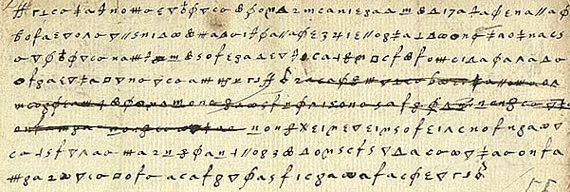
\includegraphics[width=\linewidth, height=1.5in, keepaspectratio]{../figure/encrypted_letter.jpg}
\caption{Snippet from encrypted communication between queen Mary and Sir
Babington}
\label{maryscottletterfig}
\end{marginfigure}

Mary used what's known as a \emph{substitution cipher} where each letter
is transformed into a different obscure symbol (see
\cref{maryscottletterfig}). At a first look, such a letter might seem
rather inscrutable- a meaningless sequence of strange symbols. However,
after some thought, one might recognize that these symbols \emph{repeat}
several times and moreover that different symbols repeat with different
frequencies. Now it doesn't take a large leap of faith to assume that
perhaps each symbol corresponds to a different letter and the more
frequent symbols correspond to letters that occur in the alphabet with
higher frequency. From this observation, there is a short gap to
completely breaking the cipher, which was in fact done by queen
Elisabeth's spies who used the decoded letters to learn of all the
co-conspirators and to convict queen Mary of treason, a crime for which
she was executed. Trusting in superficial security measures (such as
using ``inscrutable'' symbols) is a trap that users of cryptography have
been falling into again and again over the years. (As in many things,
this is the subject of a great XKCD cartoon, see \cref{XKCDnavajofig}.)

\begin{marginfigure}
\centering
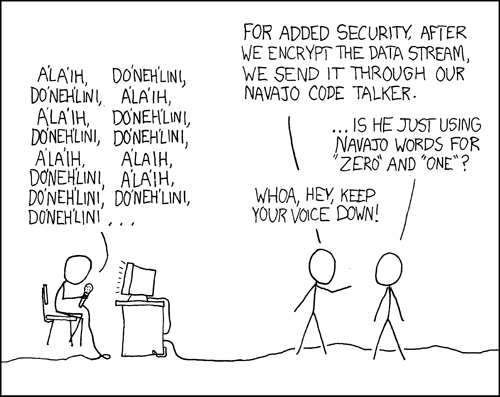
\includegraphics[width=\linewidth, height=1.5in, keepaspectratio]{../figure/code_talkers.png}
\caption{XKCD's take on the added security of using uncommon symbols}
\label{XKCDnavajofig}
\end{marginfigure}

The \href{https://en.wikipedia.org/wiki/Vigen\%C3\%A8re_cipher}{Vigenère
cipher} is named after Blaise de Vigenère who described it in a book in
1586 (though it was invented earlier by Bellaso). The idea is to use a
collection of substitution ciphers - if there are \(n\) different
ciphers then the first letter of the plaintext is encoded with the first
cipher, the second with the second cipher, the \(n^{th}\) with the
\(n^{th}\) cipher, and then the \(n+1^{st}\) letter is again encoded
with the first cipher. The key is usually a word or a phrase of \(n\)
letters, and the \(i^{th}\) substitution cipher is obtained by shifting
each letter \(k_i\) positions in the alphabet. This ``flattens'' the
frequencies and makes it much harder to do frequency analysis, which is
why this cipher was considered ``unbreakable'' for 300+ years and got
the nickname ``le chiffre indéchiffrable'' (``the unbreakable cipher'').
Nevertheless, Charles Babbage cracked the Vigenère cipher in 1854
(though he did not publish it). In 1863 Friedrich Kasiski broke the
cipher and published the result. The idea is that once you guess the
length of the cipher, you can reduce the task to breaking a simple
substitution cipher which can be done via frequency analysis (can you
see why?). Confederate generals used Vigenère regularly during the civil
war, and their messages were routinely cryptanalyzed by Union officers.

\begin{marginfigure}
\centering
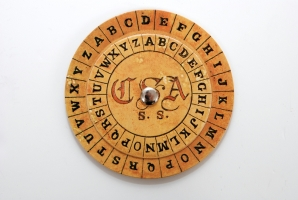
\includegraphics[width=\linewidth, height=1.5in, keepaspectratio]{../figure/confederate_cipher_disk.jpg}
\caption{Confederate Cipher Disk for implementing the Vigenère cipher}
\label{tmplabelfig}
\end{marginfigure}

\begin{marginfigure}
\centering
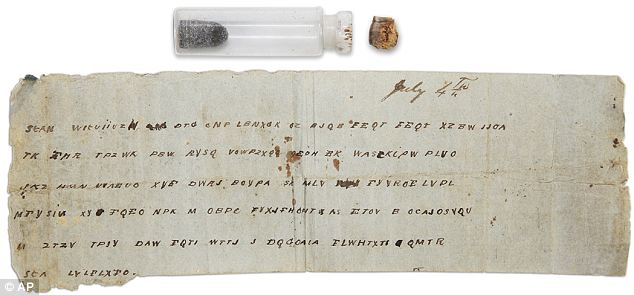
\includegraphics[width=\linewidth, height=1.5in, keepaspectratio]{../figure/confederate_message.jpg}
\caption{Confederate encryption of the message ``Gen'l Pemberton: You
can expect no help from this side of the river. Let Gen'l Johnston know,
if possible, when you can attack the same point on the enemy's lines.
Inform me also and I will endeavor to make a diversion. I have sent some
caps. I subjoin a despatch from General Johnston.''}
\label{tmplabelfig}
\end{marginfigure}

The \emph{Enigma} cipher was a mechanical cipher (looking like a
typewriter, see \cref{enigmafig}) where each letter typed would get
mapped into a different letter depending on the (rather complicated) key
and current state of the machine which had several rotors that rotated
at different paces. An identically wired machine at the other end could
be used to decrypt. Just as many ciphers in history, this has also been
believed by the Germans to be ``impossible to break'' and even quite
late in the war they refused to believe it was broken despite mounting
evidence to that effect. (In fact, some German generals refused to
believe it was broken even \emph{after} the war.) Breaking Enigma was an
heroic effort which was initiated by the Poles and then completed by the
British at Bletchley Park, with Alan Turing (of the Turing machines)
playing a key role. As part of this effort the Brits built arguably the
world's first large scale mechanical computation devices (though they
looked more similar to washing machines than to iPhones). They were also
helped along the way by some quirks and errors of the German operators.
For example, the fact that their messages ended with ``Heil Hitler''
turned out to be quite useful.

\begin{marginfigure}
\centering
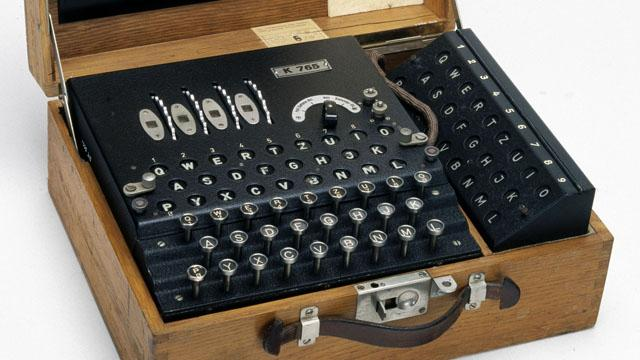
\includegraphics[width=\linewidth, height=1.5in, keepaspectratio]{../figure/enigma.jpg}
\caption{In the \emph{Enigma} mechanical cipher the secret key would be
the settings of the rotors and internal wires. As the operator types up
their message, the encrypted version appeared in the display area above,
and the internal state of the cipher was updated (and so typing the same
letter twice would generally result in two different letters output).
Decrypting follows the same process: if the sender and receiver are
using the same key then typing the ciphertext would result in the
plaintext appearing in the display.}
\label{enigmafig}
\end{marginfigure}

Here is one entertaining anecdote: the Enigma machine would never map a
letter to itself. In March 1941, Mavis Batey, a cryptanalyst at
Bletchley Park received a very long message that she tried to decrypt.
She then noticed a curious property--- the message did \emph{not}
contain the letter ``L''.\footnote{Here is a nice exercise: compute (up
  to an order of magnitude) the probability that a 50-letter long
  message composed of random letters will end up not containing the
  letter ``L''.} She realized that the probability that no ``L'''s
appeared in the message is too small for this to happen by chance. Hence
she surmised that the original message must have been composed
\emph{only} of L's. That is, it must have been the case that the
operator, perhaps to test the machine, have simply sent out a message
where he repeatedly pressed the letter ``L''. This observation helped
her decode the next message, which helped inform of a planned Italian
attack and secure a resounding British victory in what became known as
``the Battle of Cape Matapan''. Mavis also helped break another Enigma
machine. Using the information she provided, the Brits were able to feed
the Germans with the false information that the main allied invasion
would take place in Pas de Calais rather than on Normandy.

In the words of General Eisenhower, the intelligence from Bletchley park
was of ``priceless value''. It made a huge difference for the Allied war
effort, thereby shortening World War II and saving millions of lives.
See also \href{http://www.cix.co.uk/~klockstone/hinsley.htm}{this
interview with Sir Harry Hinsley}.

\section{Defining encryptions}\label{1-Defining-encryptions}

Many of the troubles that cryptosystem designers faced over history (and
still face!) can be attributed to not properly defining or understanding
what the goals they want to achieve are in the first place. We now turn
to actually defining what is an encryption scheme. Clearly we can encode
every message as a string of bits, i.e., an element of \(\{0,1\}^\ell\)
for some \(\ell\). Similarly, we can encode the \emph{key} as a string
of bits as well, i.e., an element of \(\{0,1\}^n\) for some \(n\). Thus,
we can think of an encryption scheme as composed of two functions. The
\emph{encryption function} \(E\) maps a secret key \(k \in \{0,1\}^n\)
and a message (known also as \emph{plaintext}) \(m\in \{0,1\}^\ell\)
into a \emph{ciphertext} \(c \in \{0,1\}^L\) for some \(L\). We write
this as \(c = E_k(m)\). The \emph{decryption function} \(D\) does the
reverse operation, mapping the secret key \(k\) and the ciphertext \(c\)
back into the plaintext message \(m\), which we write as \(m = D_k(c)\).
The basic equation is that if we use the same key for encryption and
decryption, then we should get the same message back. That is, for every
\(k \in \{0,1\}^n\) and \(m\in \{0,1\}^\ell\),

\begin{equation*}
m = D_k(E_k(m)) \;.
\end{equation*}

This motivates the following definition which attempts to capture what
it means for an encryption scheme to be \emph{valid} or ``make sense'',
regardless of whether or not it is \emph{secure}:

\hypertarget{encryptiondef}{}
\begin{definition}[Valid encryption scheme] \label[definition]{encryptiondef}

Let \(\ell:\N \rightarrow \N\) and \(C:\N \rightarrow \N\) be two
functions mapping natural numbers to natural numbers. A pair of
polynomial-time computable functions \((E,D)\) mapping strings to
strings is a \emph{valid private key encryption scheme} (or
\emph{encryption scheme} for short) with plaintext length function
\(\ell(\cdot)\) and ciphertext length function \(C(\cdot)\) if for every
\(n\in \N\), \(k\in \{0,1\}^n\) and \(m \in \{0,1\}^{\ell(n)}\),
\(|E_k(m)|= C(n)\) and \[
D(k,E(k,m))=m \;. \label{eqvalidenc}
\]

\end{definition}

We will often write the first input (i.e., the key) to the encryption
and decryption as a subscript and so can write \eqref{eqvalidenc} also
as \(D_k(E_k(m))=m\).

\begin{figure}
\centering
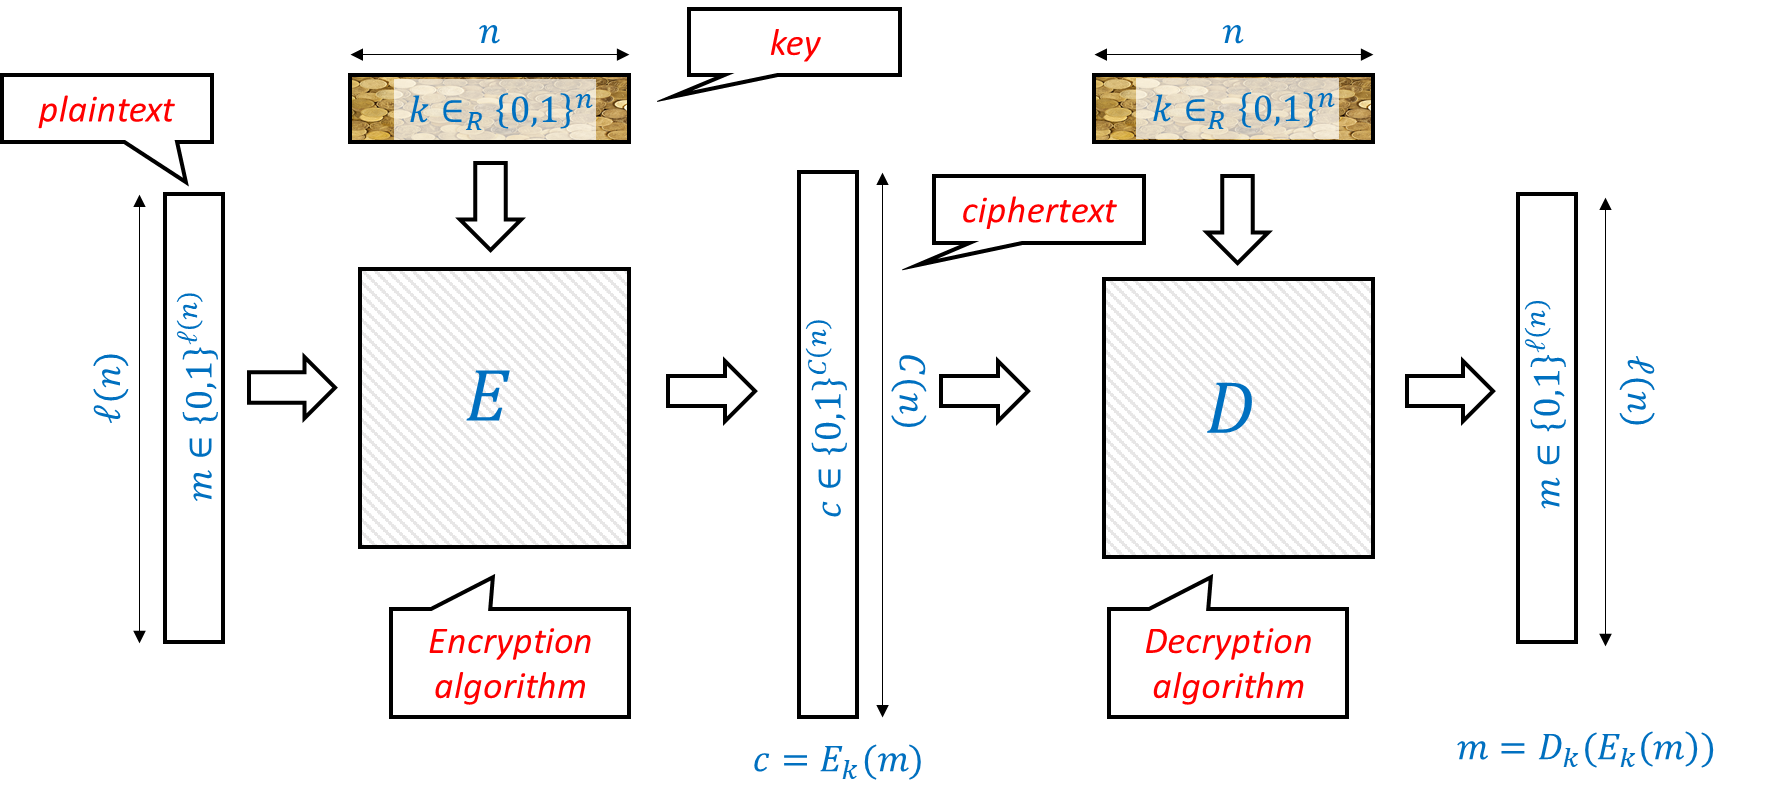
\includegraphics[width=\textwidth, height=0.25\paperheight, keepaspectratio]{../figure/valid_encryption_fig.png}
\caption{A private-key encryption scheme is a pair of algorithms \(E,D\)
such that for every key \(k\in \{0,1\}^n\) and plaintext
\(x\in \{0,1\}^{\ell(n)}\), \(c=E_k(m)\) is a ciphertext of length
\(C(n)\). The encryption scheme is \emph{valid} if for every such \(y\),
\(D_k(y)=x\). That is, the decryption of an encryption of \(x\) is
\(x\), as long as both encryption and decryption use the same key.}
\label{validencryption}
\end{figure}

The validity condition implies that for any fixed \(k\), the map
\(m \mapsto E_k(m)\) is one to one (can you see why?) and hence the
ciphertext length is always at least the plaintext length. Thus we
typically focus on the plaintext length as the quantity to optimize in
an encryption scheme. The \emph{larger} \(\ell(n)\) is, the better the
scheme, since it means we need a shorter secret key to protect messages
of the same length.

\hypertarget{notation}{}
\begin{remark}[A note on notation, and comparison with Katz-Lindell, Boneh-Shoup, and other texts.] \label[remark]{notation}

\emph{A note on notation:} We will always use \(i,j,\ell,n\) to denote
natural numbers.

The number \(n\) will often denote the length of our secret key. The
length of the key (or another closely related number) is often known as
the \emph{security parameter} in the literature. Katz-Lindell also uses
\(n\) to denote this parameter, while Boneh-Shoup and Rosulek use
\(\lambda\) for it. (Some texts also use the Greek letter \(\kappa\) for
the same parameter.) We chose to denote the security parameter by \(n\)
as to correspond with the standard algorithmic notation for input length
(as in \(O(n)\) or \(O(n^2)\) time algorithms).

We often use \(\ell\) to denote the length of the message, sometimes
also known as ``block length'' since longer messages are simply chopped
into ``blocks'' of length \(\ell\) and also appropriately padded.

We will use \(k\) to denote the secret key, \(m\) to denote the secret
plaintext message, and \(c\) to denote the encrypted ciphertext. Note
that \(k,m,c\) are not numbers but rather bit strings of lengths
\(n,\ell(n),C(n)\) respectively. We will also sometimes use \(x\) and
\(y\) to denote strings, and so sometimes use \(x\) as the plaintext and
\(y\) as the ciphertext. In general, while we try to reserve variable
names for particular purposes, cryptography uses so many concepts that
it would sometimes need to ``reuse'' the same letter for different
purposes.

For simplicity, we denote the space of possible keys as \(\{0,1\}^n\)
and the space of possible messages as \(\{0,1\}^\ell\) for
\(\ell=\ell(n)\). Boneh-Shoup uses a more general notation of
\(\mathcal{K}\) for the space of all possible keys and \(\mathcal{M}\)
for the space of all possible messages. This does not make much
difference since we can represent every discrete object such as a key or
message as a binary string. (One difference is that in principle the
space of all possible messages could include messages of unbounded
length, though in such a case what is done in both theory and practice
is to break these up into finite-size blocks and encrypt one block at a
time.)

\end{remark}

\section{Defining security of
encryption}\label{1-Defining-security-of-e}

\cref{encryptiondef} says nothing about security and does not rule out
trivial ``encryption'' schemes such as the scheme \(E_k(m) = m\) that
simply outputs the plaintext as is. Defining security is tricky, and
we'll take it one step at a time, but let's start by pondering what is
secret and what is not. A priori we are thinking of an attacker Eve that
simply sees the ciphertext \(c=E_k(m)\) and does not know anything on
how it was generated. So, it does not know the details of \(E\) and
\(D\), and certainly does not know the secret key \(k\). However, many
of the troubles past cryptosystems went through were caused by them
relying on ``security through obscurity''--- trusting that the fact
their \emph{methods} are not known to their enemy will protect them from
being broken. This is a faulty assumption - if you reuse a method again
and again (even with a different key each time) then eventually your
adversaries will figure out what you are doing. And if Alice and Bob
meet frequently in a secure location to decide on a new method, they
might as well take the opportunity to exchange their secret
messages\ldots{}

These considerations led Auguste Kerckhoffs in 1883 to state the
following principle:

\begin{quote}
\emph{A cryptosystem should be secure even if everything about the
system, except the key, is public knowledge.}\footnote{The actual quote
  is ``Il faut qu'il n'exige pas le secret, et qu'il puisse sans
  inconvénient tomber entre les mains de l'ennemi'' loosely translated
  as ``The system must not require secrecy and can be stolen by the
  enemy without causing trouble''. According to Steve Bellovin the NSA
  version is ``assume that the first copy of any device we make is
  shipped to the Kremlin''.}
\end{quote}

Why is it OK to assume the key is secret and not the algorithm? Because
we can always choose a fresh key. But of course that won't help us much
if our key is ``1234'' or ``passw0rd!''. In fact, if you use \emph{any}
deterministic algorithm to choose the key then eventually your adversary
will figure this out. Therefore for security we must choose the key at
\emph{random} and can restate Kerckhoffs's principle as follows:

\begin{quote}
\emph{There is no secrecy without randomness}
\end{quote}

This is such a crucial point that is worth repeating:

\begin{quote}
\emph{There is no secrecy without randomness}
\end{quote}

At the heart of every cryptographic scheme there is a secret key, and
the secret key is always chosen at random. A corollary of that is that
to understand cryptography, you need to know some probability theory.
Fortunately, we don't need much of probability- only probability over
finite spaces, and basic notions such as expectation, variance,
concentration and the union bound suffice for most of we need. In fact,
understanding the following two statements will already get you much of
what you need for cryptography:

\begin{itemize}
\item
  For every fixed string \(x\in\{0,1\}^n\), if you toss a coin \(n\)
  times, the probability that the heads/tails pattern will be exactly
  \(x\) is \(2^{-n}\).
\item
  A probability of \(2^{-128}\) is really really small.
\end{itemize}

\subsection{Generating randomness in actual cryptographic
systems}\label{1-Generating-randomness-}

How do we actually get random bits in actual systems? The main idea is
to use a two stage approach. First we need to get some data that is
\emph{unpredictable} from the point of view of an attacker on our
system. Some sources for this could be measuring latency on the network
or hard drives (getting harder with solid state disk), user keyboard and
mouse movement patterns (problematic when you need fresh randomness at
boot time ), clock drift and more, there are some other sources
including audio, video, and network. All of these can be problematic,
especially for servers or virtual machines, and so hardware based random
number generators based on phenomena such as thermal noise or nuclear
decay are becoming more popular. Once we have some data \(X\) that is
unpredictable, we need to estimate the \emph{entropy} in it. You can
roughly imagine that \(X\) has \(k\) bits of entropy if the probability
that an attacker can guess \(X\) is at most \(2^{-k}\). People then use
a \emph{hash function} (an object we'll talk about more later) to map
\(X\) into a string of length \(k\) which is then hopefully distributed
(close to) uniformly at random. All of this process, and especially
understanding the amount of information an attacker may have on the
entropy sources, is a bit of a dark art and indeed a number of attacks
on cryptographic systems were actually enabled by weak generation of
randomness. Here are a few examples.

One of the first attacks was on the SSL implementation of Netscape
(\emph{the} browser at the time). Netscape used the following
``unpredictable'' information--- the time of day and a process ID both
of which turned out to be quite predictable (who knew attackers have
clocks too?). Netscape tried to protect its security through ``security
through obscurity'' by not releasing the source code for their
pseudorandom generator, but it was reverse engineered by
\href{https://www.cs.berkeley.edu/~daw/papers/ddj-netscape.html}{Ian
Goldberg and David Wagner} (Ph.D students at the time) who demonstrated
this attack.

In 2006 a programmer removed a line of code from the procedure to
generate entropy in OpenSSL package distributed by Debian since it
caused a warning in some automatic verification code. As a result for
two years (until this was discovered) all the randomness generated by
this procedure used only the process ID as an ``unpredictable'' source.
This means that all communication done by users in that period is fairly
easily breakable (and in particular, if some entities recorded that
communication they could break it also retroactively). This caused a
huge headache and a worldwide regeneration of keys, though it is
believed that many of the weak keys are still used. See
\href{http://www.xkcd.com/424/}{XKCD's take} on that incident.

\begin{marginfigure}
\centering
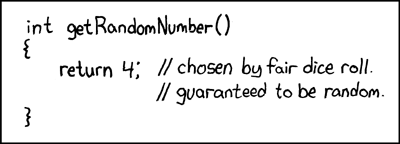
\includegraphics[width=\linewidth, height=1.5in, keepaspectratio]{../figure/random_number.png}
\caption{XKCD Cartoon: Random number generator}
\label{tmplabelfig}
\end{marginfigure}

In 2012 two separate teams of researchers scanned a large number of RSA
keys on the web and found out that about 4 percent of them are easy to
break. The main issue were devices such as routers, internet-connected
printers and such. These devices sometimes run variants of Linux- a
desktop operating system- but without a hard drive, mouse or keyboard,
they don't have access to many of the entropy sources that desktops
have. Coupled with some good old fashioned ignorance of cryptography and
software bugs, this led to many keys that are downright trivial to
break, see
\href{https://freedom-to-tinker.com/blog/nadiah/new-research-theres-no-need-panic-over-factorable-keys-just-mind-your-ps-and-qs/}{this
blog post} and \href{https://factorable.net/}{this web page} for more
details.

After the entropy is collected and then ``purified'' or ``extracted'' to
a uniformly random string that is, say, a few hundred bits long, we
often need to ``expand'' it into a longer string that is also uniform
(or at least looks like that for all practical purposes). We will
discuss how to go about that in the next lecture. This step has its
weaknesses too, and in particular the Snowden documents, combined with
observations of Shumow and Ferguson, strongly suggest that the NSA has
deliberately inserted a \emph{trapdoor} in one of the pseudorandom
generators published by the National Institute of Standards and
Technologies (NIST). Fortunately, this generator wasn't widely adopted,
but apparently the NSA did pay 10 million dollars to RSA security so the
latter would make this generator their default option in their products.

\section{Defining the secrecy
requirement.}\label{1-Defining-the-secrecy-r}

Defining the secrecy requirement for an encryption is not simple. Over
the course of history, many smart people got it wrong and convinced
themselves that ciphers were impossible to break. The first person to
truly ask the question in a rigorous way was Claude Shannon in 1945
(though a partial version of his manuscript was only declassified in
1949). Simply by asking this question, he made an enormous contribution
to the science of cryptography and practical security. We now will try
to examine how one might answer it.

Let me warn you ahead of time that we are going to insist on a
\emph{mathematically precise definition} of security. That means that
the definition must capture security in all cases, and the existence of
a single counterexample, no matter how ``silly'', would make us rule out
a candidate definition. This exercise of coming up with ``silly''
counterexamples might seem, well, silly. But in fact it is this method
that has led Shannon to formulate his theory of secrecy, which (after
much followup work) eventually revolutionized cryptography, and brought
this science to a new age where Edgar Allan Poe's maxim no longer holds,
and we are able to design ciphers which human (or even nonhuman)
ingenuity cannot break.

The most natural way to attack an encryption is for Eve to guess all
possible keys. In many encryption schemes this number is enormous and
this attack is completely infeasible. For example, the theoretical
number of possibilities in the Enigma cipher was about \(10^{113}\)
which roughly means that even if we filled the milky way galaxy with
computers operating at light speed, the sun would still die out before
it finished examining all the possibilities.\footnote{There are about
  \(10^{68}\) atoms in the galaxy, so even if we assumed that each one
  of those atoms was a computer that can process say \(10^{21}\)
  decryption attempts per second (as the speed of light is \(10^9\)
  meters per second and the diameter of an atom is about \(10^{-12}\)
  meters), then it would still take \(10^{113-89} = 10^{24}\) seconds,
  which is about \(10^{17}\) years to exhaust all possibilities, while
  the sun is estimated to burn out in about 5 billion years.} One can
understand why the Germans thought it was impossible to break. (Note
that despite the number of possibilities being so enormous, such a key
can still be easily specified and shared between Alice and Bob by
writing down \(113\) digits on a piece of paper.) Ray Miller of the NSA
had calculated that, in the way the Germans used the machine, the number
of possibilities was ``only'' \(10^{23}\), but this is still extremely
difficult to pull off even today, and many orders of magnitudes above
the computational powers during the WW-II era. Thus clearly, it is
sometimes possible to break an encryption without trying all
possibilities. A corollary is that having a huge number of key
combinations does not guarantee security, as an attacker might find a
shortcut (as the allies did for Enigma) and recover the key without
trying all options.

Since it is possible to recover the key with some tiny probability
(e.g.~by guessing it at random), perhaps one way to define security of
an encryption scheme is that an attacker can never recover the key with
probability significantly higher than that. Here is an attempt at such a
definition:

\hypertarget{securefirstattemptdef}{}
\begin{definition}[Security of encryption: first attempt] \label[definition]{securefirstattemptdef}

An encryption scheme \((E,D)\) is \emph{\(n\)-secure} if no matter what
method Eve employs, the probability that she can recover the true key
\(k\) from the ciphertext \(c\) is at most \(2^{-n}\).

\end{definition}

\begin{pause} \label[pause]{1-When-you-see-a-mathema}

When you see a mathematical definition that attempts to model some
real-life phenomenon such as security, you should pause and ask
yourself:

\begin{enumerate}
\def\labelenumi{\arabic{enumi}.}
\item
  Do I understand mathematically what the definition is stating?\\
\item
  Is it a reasonable way to capture the real life phenomenon we are
  discussing?
\end{enumerate}

One way to answer question 2 is to try to think of both examples of
objects that satisfy the definition and examples of objects that violate
it, and see if this conforms to your intuition about whether these
objects display the phenomenon we are trying to capture. Try to do this
for \cref{securefirstattemptdef}

\end{pause}

You might wonder if \cref{securefirstattemptdef} is not \emph{too
strong}. After all how are we going to ever prove that Eve cannot
recover the secret key no matter what she does? Edgar Allan Poe would
say that there can always be a method that we overlooked. However, in
fact this definition is too \emph{weak}! Consider the following
encryption: the secret key \(k\) is chosen at random in \(\{0,1\}^n\)
but our encryption scheme simply ignores it and lets \(E_k(m)=m\) and
\(D_k(c)=c\). This is a valid encryption since \(D_k(E_k(m))=m\), but is
of course completely insecure as we are simply outputting the plaintext
in the clear. Yet, no matter what Eve does, if she only sees \(c\) and
not \(k\), there is no way she can guess the true value of \(k\) with
probability better than \(2^{-n}\), since it was chosen completely at
random and she gets no information about it. Formally, one can prove the
following result:

\hypertarget{trivialsec}{}
\begin{lemma} \label[lemma]{trivialsec}

Let \((E,D)\) be the encryption scheme above. For every function
\(Eve:\{0,1\}^\ell\rightarrow \{0,1\}^n\) and for every
\(m\in \{0,1\}^\ell\), the probability that \(Eve(E_k(m))=k\) is exactly
\(2^{-n}\).

\end{lemma}

\begin{proof} \label[proof]{1-This-follows-because-E}

This follows because \(E_k(m)=m\) and hence \(Eve(E_k(m))=Eve(m)\) which
is some fixed value \(k'\in\{0,1\}^n\) that is independent of \(k\).
Hence the probability that \(k=k'\) is \(2^{-n}\). QED

\end{proof}

The math behind the above argument is very simple, yet I urge you to
read and re-read the last two paragraphs until you are sure that you
completely understand why this encryption is in fact secure according to
the above definition. This is a ``toy example'' of the kind of reasoning
that we will be employing constantly throughout this course, and you
want to make sure that you follow it.

So, \cref{trivialsec} is true, but one might question its meaning.
Clearly this silly example was not what we meant when stating this
definition. However, as mentioned above, we are not willing to ignore
even silly examples and must amend the definition to rule them out. One
obvious objection is that we don't care about hiding the key- it is the
\emph{message} that we are trying to keep secret. This suggests the next
attempt:

\hypertarget{securesecondattemptdef}{}
\begin{definition}[Security of encryption: second attempt] \label[definition]{securesecondattemptdef}

An encryption scheme \((E,D)\) is \emph{\(n\)-secure} if for every
message \(m\) no matter what method Eve employs, the probability that
she can recover \(m\) from the ciphertext \(c=E_k(m)\) is at most
\(2^{-n}\).

\end{definition}

Now this seems like it captures our intended meaning. But remember that
we are being anal, and truly insist that the definition holds as stated,
namely that for every plaintext message \(m\) and every function
\(Eve:\{0,1\}^C\rightarrow\{0,1\}^\ell\), the probability over the
choice of \(k\) that \(Eve(E_k(m))=m\) is at most \(2^{-n}\). But now we
see that this is clearly impossible. After all, this is supposed to work
for \emph{every} message \(m\) and \emph{every} function \(Eve\), but
clearly if \(m\) is the all-zeroes message \(0^\ell\) and \(Eve\) is the
function that ignores its input and simply outputs \(0^\ell\), then it
will hold that \(Eve(E_k(m))=m\) with probability one.

So, if before the definition was too weak, the new definition is too
strong and is impossible to achieve. The problem is that of course we
could guess a fixed message with probability one, so perhaps we could
try to consider a definition with a \emph{random} message. That is:

\hypertarget{securethirdattemptdef}{}
\begin{definition}[Security of encryption: third attempt] \label[definition]{securethirdattemptdef}

An encryption scheme \((E,D)\) is \emph{\(n\)-secure} if no matter what
method Eve employs, if \(m\) is chosen at random from \(\{0,1\}^\ell\),
the probability that she can recover \(m\) from the ciphertext
\(c=E_k(m)\) is at most \(2^{-n}\).

\end{definition}

This weakened definition can in fact be achieved, but we have again
weakened it too much. Consider an encryption that hides the last
\(\ell/2\) bits of the message, but completely reveals the first
\(\ell/2\) bits. The probability of guessing a random message is
\(2^{-\ell/2}\), and so such a scheme would be ``\(\ell/2\) secure'' per
\cref{securethirdattemptdef} but this is still a scheme that you would
not want to use. The point is that in practice we don't encrypt random
messages--- our messages might be in English, might have common headers,
and might have even more structures based on the context. In fact, it
may be that the message is either ``Yes'' or ``No'' (or perhaps either
``Attack today'' or ``Attack tomorrow'') but we want to make sure Eve
doesn't learn which one it is. So, using an encryption scheme that
reveals the first half of the message (or frankly even only the first
bit) is unacceptable.

\section{Perfect Secrecy}\label{1-Perfect-Secrecy}

So far all of our attempts at definitions oscillated between being too
strong (and hence impossible) or too weak (and hence not guaranteeing
actual security). The key insight of Shannon was that in a secure
encryption scheme the ciphertext should not reveal \emph{any additional
information} about the plaintext. So, if for example it was a priori
possible for Eve to guess the plaintext with some probability \(1/k\)
(e.g., because there were only \(k\) possibilities for it) then she
should not be able to guess it with higher probability after seeing the
ciphertext. This can be formalized as follows:

\hypertarget{perfectsecrecydef}{}
\begin{definition}[Perfect secrecy] \label[definition]{perfectsecrecydef}

An encryption scheme \((E,D)\) is \emph{perfectly secret} if there for
every set \(M\subseteq\{0,1\}^\ell\) of plaintexts, and for every
strategy used by Eve, if we choose at random \(m\in M\) and a random key
\(k\in\{0,1\}^n\), then the probability that Eve guesses \(m\) after
seeing \(E_k(m)\) is at most \(1/|M|\).

\end{definition}

In particular, if we encrypt either ``Yes'' or ``No'' with probability
\(1/2\), then Eve won't be able to guess which one it is with
probability better than half. In fact, that turns out to be the heart of
the matter:

\hypertarget{twotomanythm}{}
\begin{theorem}[Two to many theorem] \label[theorem]{twotomanythm}

An encryption scheme \((E,D)\) is perfectly secret if and only if for
every two distinct plaintexts \(\{m_0,m_1\} \subseteq \{0,1\}^\ell\) and
every strategy used by Eve, if we choose at random \(b\in\{0,1\}\) and a
random key \(k\in\{0,1\}^n\), then the probability that Eve guesses
\(m_b\) after seeing \(E_k(m_b)\) is at most \(1/2\).

\end{theorem}

\begin{proof} \label[proof]{1-The-only-if-direction-}

The ``only if'' direction is obvious--- this condition is a special case
of the perfect secrecy condition for a set \(M\) of size \(2\).

The ``if'' direction is trickier. We will use a proof by contradiction.
We need to show that if there is some set \(M\) (of size possibly much
larger than \(2\)) and some strategy for Eve to guess (based on the
ciphertext) a plaintext chosen from \(M\) with probability larger than
\(1/|M|\), then there is also some set \(M'\) of size two and a strategy
\(Eve'\) for Eve to guess a plaintext chosen from \(M'\) with
probability larger than \(1/2\).

Let's fix the message \(m_0\) to be the all zeroes message and pick
\(m_1\) at random in \(M\). Under our assumption, it holds that for
random key \(k\) and message \(m_1\in M\),
\[\Pr_{k \leftarrow_R \{0,1\}^n, m_1 \leftarrow_R M}[Eve(E_k(m_1))=m_1] > 1/|M|\;. \label{eqabovetrivialcipher}\]
On the other hand, for every choice of \(k\), \(m'= Eve(E_k(m_0))\) is a
fixed string independent on the choice of \(m_1\), and so if we pick
\(m_1\) at random in \(M\), then the probability that \(m_1=m'\) is at
most \(1/|M|\), or in other words

\[\Pr_{k \leftarrow_R \{0,1\}^n, m_1 \leftarrow_R M}[Eve(E_k(m_0))=m_1] \leq 1/|M|\;. \label{eqhitcipher}\]

We can also write \eqref{eqabovetrivialcipher} and \eqref{eqhitcipher}
as
\begin{equation*}
\E_{m_1 \leftarrow_R M} \Pr[ Eve(E_k(m_1))=m_1] > 1/|M|
\end{equation*}
and
\begin{equation*}
\E_{m_1 \leftarrow_R M} \Pr[ Eve(E_k(m_0))=m_1] \leq 1/|M|
\end{equation*}
where these expectations are taken over the choice of \(m_1\). Hence by
linearity of expectation \[
\E_{m_1 \leftarrow_R M} \left( \Pr[ Eve(E_k(m_1))=m_1] - \Pr[ Eve(E_k(m_0))=m_1] \right) > 0 \;. \label{eqadvantageciphermonevsmzero}
\] (In words, for random \(m_1\), the probability that Eve outputs
\(m_1\) given an encryption of \(m_1\) is higher than the probability
that Eve outputs \(m_1\) given an encryption of \(m_0\).)

In particular, by the \emph{averaging argument} (the argument that if
the average of numbers is larger than \(\alpha\) then one of the numbers
is larger than \(\alpha\)) there must \emph{exist} \(m_1 \in M\)
satisfying
\begin{equation*}
\Pr[Eve(E_k(m_1))=m_1] > \Pr[Eve(E_k(m_0))=m_1] \;.
\end{equation*}
(Can you see why? This is worthwhile stopping and reading again.)

But this can be turned into an attacker \(Eve'\) such that for
\(b \leftarrow_R \{0,1\}\). the probability that \(Eve'(E_k(m_b))=m_b\)
is larger than \(1/2\). Indeed, we can define \(Eve'(c)\) to output
\(m_1\) if \(Eve(c)=m_1\) and otherwise output a random message in
\(\{ m_0 , m_1 \}\). The probability that \(Eve'(y)\) equals \(m_1\) is
higher when \(c=E_k(m_1)\) than when \(c=E_k(m_0)\), and since \(Eve'\)
outputs either \(m_0\) or \(m_1\), this means that the probability that
\(Eve'(E_k(m_b))=m_b\) is larger than \(1/2\). (Can you see why?)

\end{proof}

\begin{pause} \label[pause]{1-The-proof-of-creftwoto}

The proof of \cref{twotomanythm} is not trivial, and is worth reading
again and making sure you understand it. An excellent exercise, which I
urge you to pause and do now is to prove the following: \((E,D)\) is
perfectly secret if for every plaintexts \(m,m' \in \{0,1\}^\ell\), the
two random variables \(\{ E_k(m) \}\) and \(\{ E_{k'}(m') \}\) (for
randomly chosen keys \(k\) and \(k'\)) have precisely the same
distribution.

\end{pause}

\hypertarget{perfectsecrecyequiv}{}
\begin{solvedexercise}[Perfect secrecy, equivalent definition] \label[solvedexercise]{perfectsecrecyequiv}

Prove that a valid encryption scheme \((E,D)\) with plaintext length
\(\ell(\cdot)\) is perfectly secret if and only if for every \(n\in \N\)
and plaintexts \(m,m' \in \{0,1\}^{\ell(n)}\), the following two
distributions \(Y\) and \(Y'\) over \(\{0,1\}^*\) are identical:

\begin{itemize}
\item
  \(Y\) is obtained by sampling \(k\leftarrow_R \{0,1\}^n\) and
  outputting \(E_k(m)\).
\item
  \(Y'\) is obtained by sampling \(k\leftarrow_R \{0,1\}^n\) and
  outputting \(E_k(m')\).
\end{itemize}

\end{solvedexercise}

\begin{solution} \label[solution]{1-We-only-sketch-the-pro}

We only sketch the proof. The condition in the exercise is equivalent to
perfect secrecy with \(|M|=2\). For every \(M = \{ m,m' \}\), if \(Y\)
and \(Y'\) are identical then clearly for every \(Eve\) and possible
output \(y\), \(\Pr[ Eve(E_k(m))=y] = \Pr[ Eve(E_k(m'))=y]\) since these
correspond applying \(Eve\) on the same distribution \(Y=Y'\). On the
other hand, if \(Y\) and \(Y'\) are not identical then there must exist
some ciphertext \(c^*\) such that \(\Pr[ Y=c^*] > \Pr[ Y'=c^*]\) (or
vice versa). The adversary that on input \(c\) guesses that \(c\) is an
encryption of \(m\) if \(c=c^*\) and otherwise tosses a coin will have
some advantage over \(1/2\) in distinguishing an encryption of \(m\)
from an encryption of \(m'\).

\end{solution}

We summarize the equivalent definitions of perfect secrecy in the
following theorem, whose (omitted) proof follows from
\cref{twotomanythm} and \cref{perfectsecrecyequiv} as well as similar
proof ideas.

\hypertarget{perfectsecrecythm}{}
\begin{theorem}[Perfect secrecy equivalent conditions] \label[theorem]{perfectsecrecythm}

Let \((E,D)\) be a valid encryption scheme with message length
\(\ell(n)\). Then the following conditions are equivalent:

\begin{enumerate}
\def\labelenumi{\arabic{enumi}.}
\item
  \((E,D)\) is perfectly secret as per \cref{perfectsecrecydef}.
\item
  For every pair of messages \(m_0,m_1 \in \{0,1\}^{\ell(n)}\), the
  distributions \(\{ E_k(m_0) \}_{k \leftarrow_R \{0,1\}^n}\) and
  \(\{ E_k(m_1) \}_{k \leftarrow_R \{0,1\}^n}\) are identical.
\item
  (Two-message security: Eve can't guess which of one of two messages
  was encrypted with success better than half.) For every function
  \(Eve:\{0,1\}^{C(n)} \rightarrow \{0,1\}^{\ell(n)}\) and pair of
  messages \(m_0,m_1 \in \{0,1\}^{\ell(n)}\),
\end{enumerate}

\begin{equation*}
\Pr_{b \leftarrow_R \{0,1\}, k \leftarrow_R \{0,1\}^n} [ Eve(E_k(m_b))=m_b ] \leq 1/2
\end{equation*}

\begin{enumerate}
\def\labelenumi{\arabic{enumi}.}
\setcounter{enumi}{3}
\tightlist
\item
  (Arbitrary prior security: Eve can't guess which message was encrypted
  with success better than her prior information.) For every
  distribution \(\mathcal{D}\) over \(\{0,1\}^{\ell(n)}\), and
  \(Eve:\{0,1\}^{C(n)} \rightarrow \{0,1\}^{\ell(n)}\),
\end{enumerate}

\begin{equation*}
\Pr_{m \leftarrow_R \mathcal{D}, k \leftarrow_R \{0,1\}^n}[ Eve(E_k(m))=m ] \leq \max(\mathcal{D})
\end{equation*}

where we denote
\(\max(\mathcal{D}) = \max_{m^*\in \{0,1\}^{\ell(n)}} \Pr_{m \leftarrow_R \mathcal{D}}[m=m^*]\)
to be the largest probability of any element under \(\mathcal{D}\).

\end{theorem}

\subsection{Achieving perfect secrecy}\label{1-Achieving-perfect-secr}

So, perfect secrecy is a natural condition, and does not seem to be too
weak for applications, but can it actually be achieved? After all, the
condition that two different plaintexts are mapped to the same
distribution seems somewhat at odds with the condition that Bob would
succeed in decrypting the ciphertexts and find out if the plaintext was
in fact \(m\) or \(m'\). It turns out the answer is yes! For example,
\cref{onetimepadtwofig} details a perfectly secret encryption for two
bits.

\begin{figure}
\centering
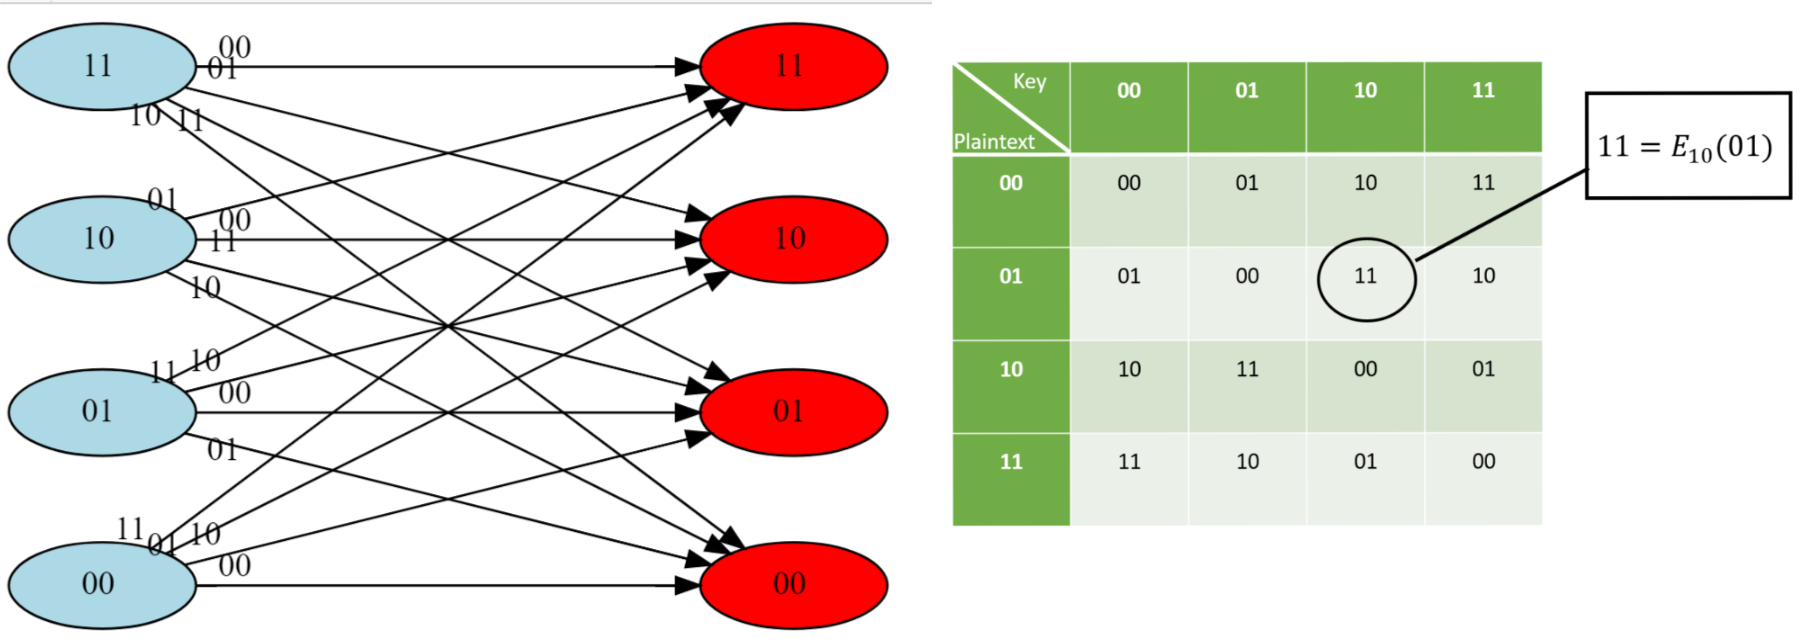
\includegraphics[width=\textwidth, height=0.25\paperheight, keepaspectratio]{../figure/onetimepadtwobits.png}
\caption{A perfectly secret encryption scheme for two-bit keys and
messages. The blue vertices represent plaintexts and the red vertices
represent ciphertexts, each edge mapping a plaintext \(m\) to a
ciphertext \(c=E_k(m)\) is labeled with the corresponding key \(k\).
Since there are four possible keys, the degree of the graph is four and
it is in fact a complete bipartite graph. The encryption scheme is valid
in the sense that for every \(k\in \{0,1\}^2\), the map
\(m \mapsto E_k(m)\) is one-to-one, which in other words means that the
set of edges labeled with \(k\) is a \emph{matching}.}
\label{onetimepadtwofig}
\end{figure}

In fact, this can be generalized to any number of bits:\footnote{The
  one-time pad is typically credited to Gilbert Vernam of Bell and
  Joseph Mauborgne of the U.S. Army Signal Corps, but Steve Bellovin
  discovered an earlier inventor
  \href{http://www.cs.columbia.edu/~CS4HS/talks/FrankMillerOneTimePad.pdf}{Frank
  Miller} who published a description of the one-time pad in 1882.
  However, it is unclear if Miller realized the fact that security of
  this system can be mathematically proven, and so the theorem below
  should probably be still be credited to Vernam and Mauborgne.}

\hypertarget{onetimepad}{}
\begin{theorem}[One Time Pad (Vernam 1917, Shannon 1949)] \label[theorem]{onetimepad}

There is a perfectly secret valid encryption scheme \((E,D)\) with
\(\ell(n)=n\).

\end{theorem}

\begin{proofidea} \label[proofidea]{1-Our-scheme-is-the-one-}

Our scheme is the
\href{https://en.wikipedia.org/wiki/One-time_pad}{one-time pad} also
known as the ``Vernam Cipher'', see \cref{onetimepadfig}. The encryption
is exceedingly simple: to encrypt a message \(m\in \{0,1\}^n\) with a
key \(k \in \{0,1\}^n\) we simply output \(m \oplus k\) where \(\oplus\)
is the bitwise XOR operation that outputs the string corresponding to
XORing each coordinate of \(m\) and \(k\).

\end{proofidea}

\begin{figure}
\centering
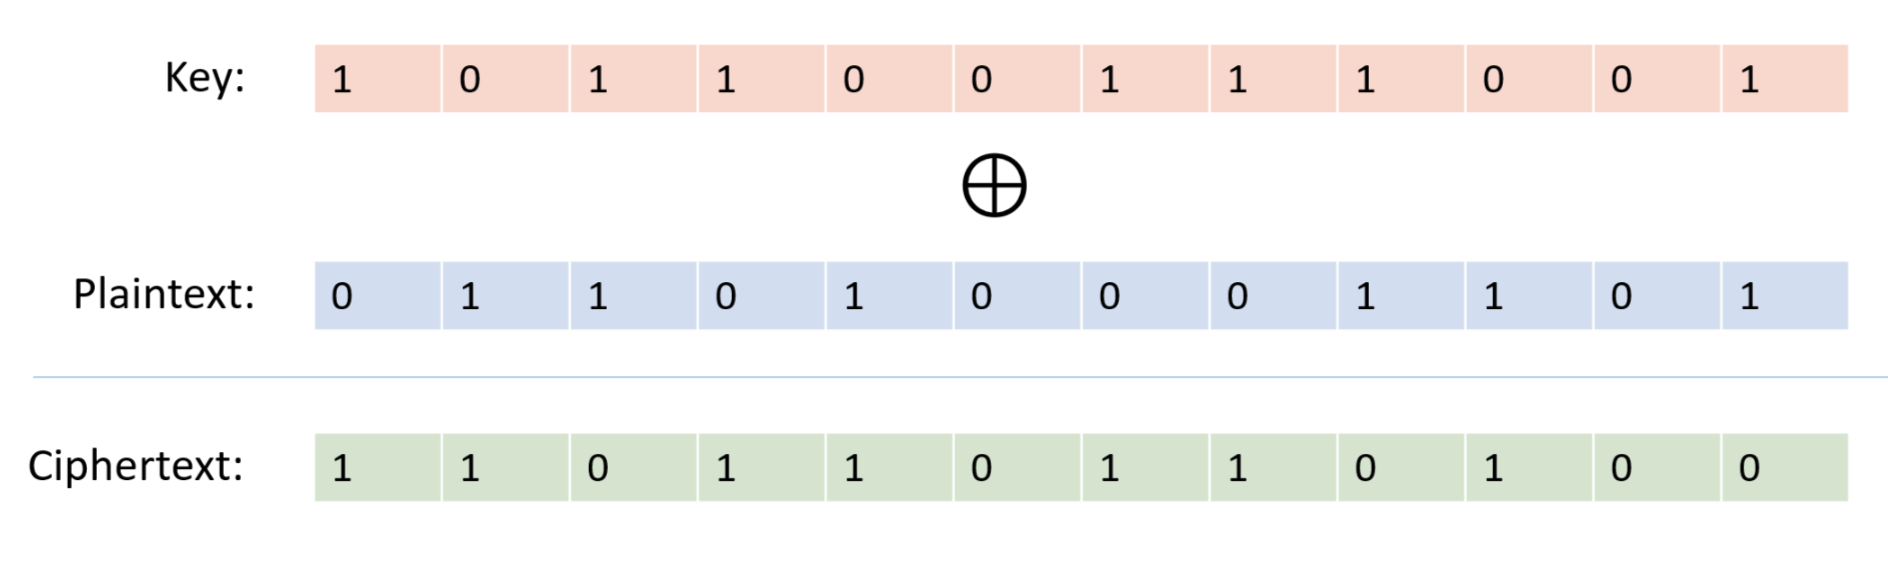
\includegraphics[width=\textwidth, height=0.25\paperheight, keepaspectratio]{../figure/onetimepad.png}
\caption{In the \emph{one time pad} encryption scheme we encrypt a
plaintext \(m\in \{0,1\}^n\) with a key \(k\in \{0,1\}^n\) by the
ciphertext \(m \oplus k\) where \(\oplus\) denotes the bitwise XOR
operation.}
\label{onetimepadfig}
\end{figure}

\begin{proof}[Proof of \cref{onetimepad}] \label[proof]{1-For-two-binary-strings}

For two binary strings \(a\) and \(b\) of the same length \(n\), we
define \(a \oplus b\) to be the string \(c \in \{0,1\}^n\) such that
\(c_i = a_i + b_i \mod 2\) for every \(i\in [n]\). The encryption scheme
\((E,D)\) is defined as follows: \(E_k(m) = m\oplus k\) and
\(D_k(c)= c \oplus k\). By the associative law of addition (which works
also modulo two),
\(D_k(E_k(m))=(m\oplus k) \oplus k = m \oplus (k \oplus k) = m \oplus 0^n = m\),
using the fact that for every bit \(\sigma \in \{0,1\}\),
\(\sigma + \sigma \mod 2 = 0\) and \(\sigma + 0 = \sigma \mod 2\). Hence
\((E,D)\) form a valid encryption.

To analyze the perfect secrecy property, we claim that for every
\(m\in \{0,1\}^n\), the distribution \(Y_m=E_k(m)\) where
\(k \leftarrow_R \{0,1\}^n\) is simply the uniform distribution over
\(\{0,1\}^n\), and hence in particular the distributions \(Y_{m}\) and
\(Y_{m'}\) are identical for every \(m,m' \in \{0,1\}^n\). Indeed, for
every particular \(y\in \{0,1\}^n\), the value \(y\) is output by
\(Y_m\) if and only if \(y = m \oplus k\) which holds if and only if
\(k= m \oplus y\). Since \(k\) is chosen uniformly at random in
\(\{0,1\}^n\), the probability that \(k\) happens to equal
\(m \oplus y\) is exactly \(2^{-n}\), which means that every string
\(y\) is output by \(Y_m\) with probability \(2^{-n}\).

\end{proof}

\begin{figure}
\centering
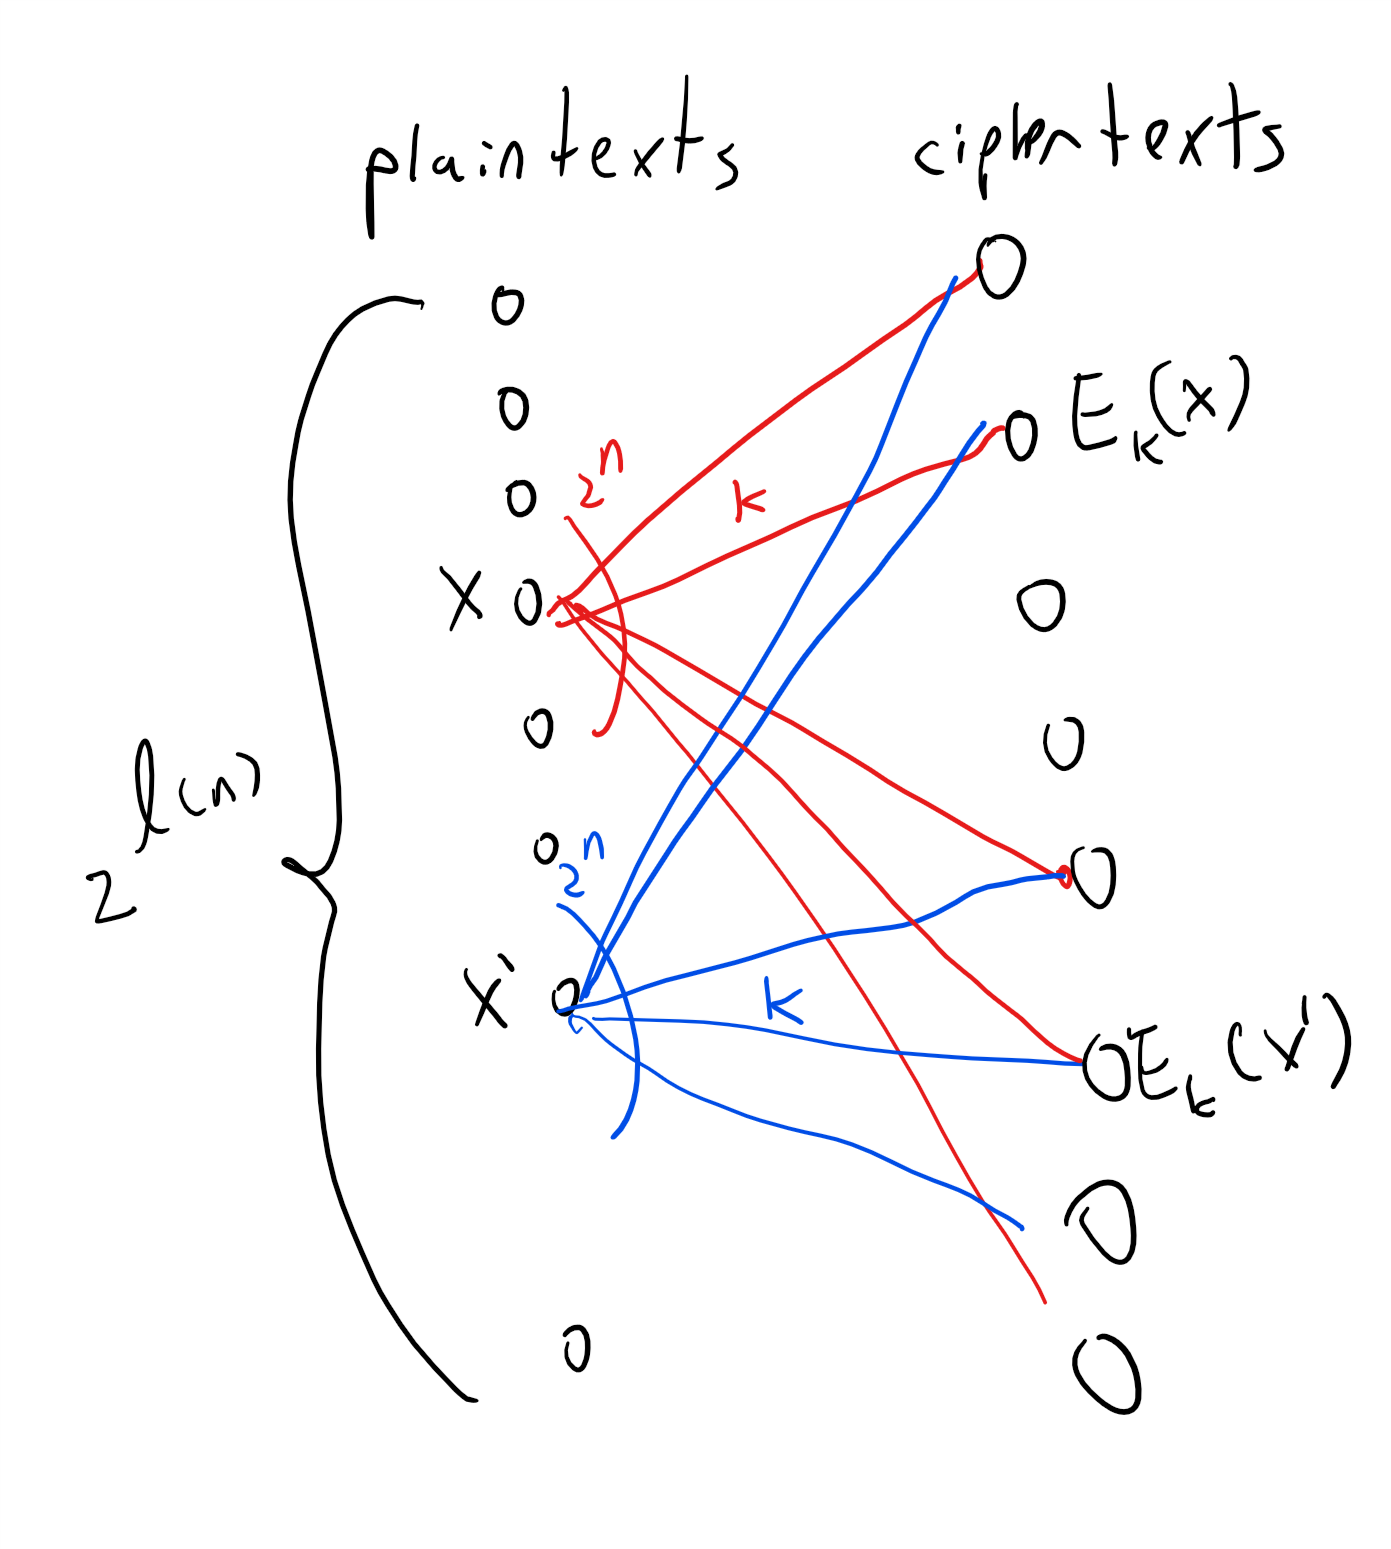
\includegraphics[width=\textwidth, height=0.25\paperheight, keepaspectratio]{../figure/perfectsecrecy.png}
\caption{For any key length \(n\), we can visualize an encryption scheme
\((E,D)\) as a graph with a vertex for every one of the \(2^{\ell(n)}\)
possible plaintexts and for every one of the ciphertexts in
\(\{0,1\}^*\) of the form \(E_k(x)\) for \(k\in \{0,1\}^n\) and
\(x\in \{0,1\}^{\ell(n)}\). For every plaintext \(x\) and key \(k\), we
add an edge labeled \(k\) between \(x\) and \(E_k(x)\). By the validity
condition, if we pick any fixed key \(k\), the map \(x \mapsto E_k(x)\)
must be one-to-one. The condition of perfect secrecy simply corresponds
to requiring that every two plaintexts \(x\) and \(x'\) have exactly the
same set of neighbors (or multi-set, if there are parallel edges).}
\label{perfectsecfig}
\end{figure}

\begin{pause} \label[pause]{1-The-argument-above-is-}

The argument above is quite simple but is worth reading again. To
understand why the one-time pad is perfectly secret, it is useful to
envision it as a bipartite graph as we've done in
\cref{onetimepadtwofig}. (In fact the encryption scheme of
\cref{onetimepadtwofig} is precisely the one-time pad for \(n=2\).) For
every \(n\), the one-time pad encryption scheme corresponds to a
bipartite graph with \(2^n\) vertices on the ``left side'' corresponding
to the plaintexts in \(\{0,1\}^n\) and \(2^n\) vertices on the ``right
side'' corresponding to the ciphertexts \(\{0,1\}^n\). For every
\(x\in \{0,1\}^n\) and \(k\in \{0,1\}^n\), we connect \(x\) to the
vertex \(y=E_k(x)\) with an edge that we label with \(k\). One can see
that this is the complete bipartite graph, where every vertex on the
left is connected to \emph{all} vertices on the right. In particular
this means that for every left vertex \(x\), the distribution on the
ciphertexts obtained by taking a random \(k\in \{0,1\}^n\) and going to
the neighbor of \(x\) on the edge labeled \(k\) is the uniform
distribution over \(\{0,1\}^n\). This ensures the perfect secrecy
condition.

\end{pause}

\section{Necessity of long keys}\label{1-Necessity-of-long-keys}

So, does \cref{onetimepad} give the final word on cryptography, and
means that we can all communicate with perfect secrecy and live happily
ever after? No it doesn't. While the one-time pad is efficient, and
gives perfect secrecy, it has one glaring disadvantage: to communicate
\(n\) bits you need to store a key of length \(n\). In contrast,
practically used cryptosystems such as AES-128 have a short key of
\(128\) bits (i.e., \(16\) bytes) that can be used to protect terabytes
or more of communication! Imagine that we all needed to use the one time
pad. If that was the case, then if you had to communicate with \(m\)
people, you would have to maintain (securely!) \(m\) huge files that are
each as long as the length of the maximum total communication you expect
with that person. Imagine that every time you opened an account with
Amazon, Google, or any other service, they would need to send you in the
mail (ideally with a secure courier) a DVD full of random numbers, and
every time you suspected a virus, you'd need to ask all these services
for a fresh DVD. This doesn't sound so appealing.

This is not just a theoretical issue. The Soviets have used the one-time
pad for their confidential communication since before the 1940's. In
fact, even before Shannon's work, the U.S. intelligence already knew in
1941 that the one-time pad is in principle ``unbreakable'' (see page 32
in the \href{http://nsarchive.gwu.edu/NSAEBB/NSAEBB278/01.PDF}{Venona
document}). However, it turned out that the hassle of manufacturing so
many keys for all the communication took its toll on the Soviets and
they ended up reusing the same keys for more than one message. They did
try to use them for completely different receivers in the (false) hope
that this wouldn't be detected. The
\href{https://en.wikipedia.org/wiki/Venona_project}{Venona Project} of
the U.S. Army was founded in February 1943 by Gene Grabeel (see
\cref{genegrabeelfig}), a former home economics teacher from Madison
Heights, Virginia and Lt. Leonard Zubko. In October 1943, they had their
breakthrough when it was discovered that the Russians were reusing their
keys. In the 37 years of its existence, the project has resulted in a
treasure chest of intelligence, exposing hundreds of KGB agents and
Russian spies in the U.S. and other countries, including Julius
Rosenberg, Harry Gold, Klaus Fuchs, Alger Hiss, Harry Dexter White and
many others.

\begin{marginfigure}
\centering
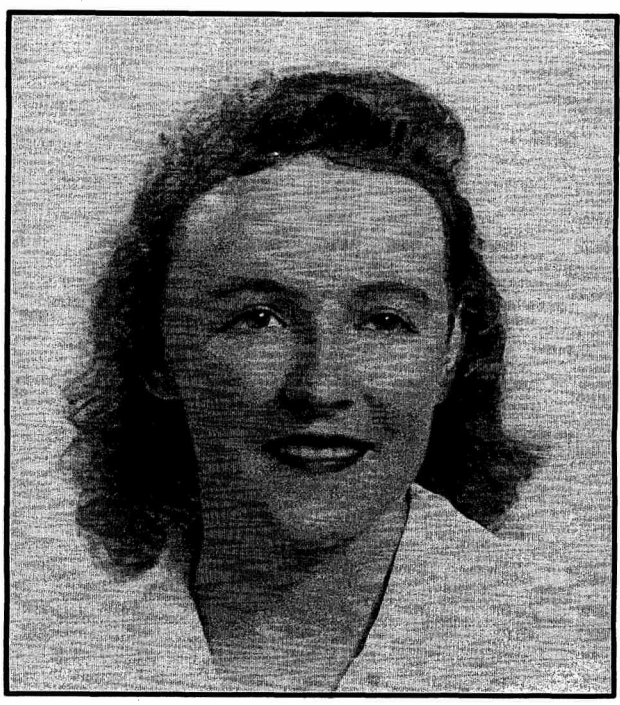
\includegraphics[width=\linewidth, height=1.5in, keepaspectratio]{../figure/genevenona.png}
\caption{Gene Grabeel, who founded the U.S. Russian SigInt program on 1
Feb 1943. Photo taken in 1942, see Page 7 in the Venona historical
study.}
\label{genegrabeelfig}
\end{marginfigure}

\begin{marginfigure}
\centering
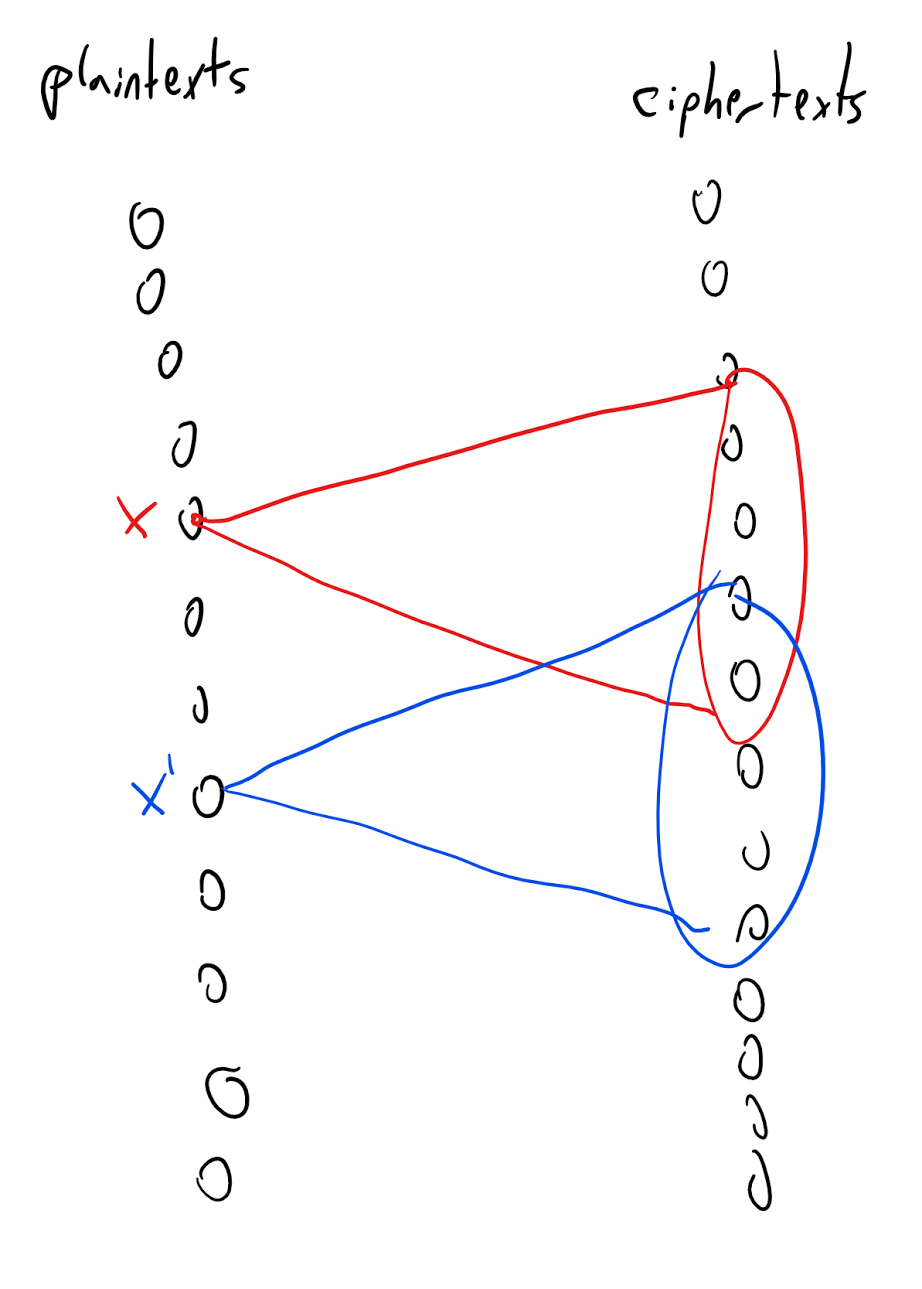
\includegraphics[width=\linewidth, height=1.5in, keepaspectratio]{../figure/longkeygraph.png}
\caption{An encryption scheme where the number of keys is smaller than
the number of plaintexts corresponds to a bipartite graph where the
degree is smaller than the number of vertices on the left side. Together
with the validity condition this implies that there will be two left
vertices \(x,x'\) with non-identical neighborhoods, and hence the scheme
does \emph{not} satisfy perfect secrecy.}
\label{longkeygraphfig}
\end{marginfigure}

Unfortunately it turns out that that such long keys are \emph{necessary}
for perfect secrecy:

\hypertarget{longkeysthm}{}
\begin{theorem}[Perfect secrecy requires long keys] \label[theorem]{longkeysthm}

For every perfectly secret encryption scheme \((E,D)\) the length
function \(\ell\) satisfies \(\ell(n) \leq n\).

\end{theorem}

\begin{proofidea} \label[proofidea]{1-The-idea-behind-the-pr}

The idea behind the proof is illustrated in \cref{longkeygraphfig}. We
define a graph between the plaintexts and ciphertexts, where we put an
edge between plaintext \(x\) and ciphertext \(y\) if there is some key
\(k\) such that \(y=E_k(x)\). The \emph{degree} of this graph is at most
the number of potential keys. The fact that the degree is smaller than
the number of plaintexts (and hence of ciphertexts) implies that there
would be two plaintexts \(x\) and \(x'\) with different sets of
neighbors, and hence the distribution of a ciphertext corresponding to
\(x\) (with a random key) will not be identical to the distribution of a
ciphertext corresponding to \(x'\).

\end{proofidea}

\begin{proof}[Proof of \cref{longkeysthm}] \label[proof]{1-Let-ED-be-a-valid-encr}

Let \(E,D\) be a valid encryption scheme with messages of length
\(\ell\) and key of length \(n<\ell\). We will show that \((E,D)\) is
not perfectly secret by providing two plaintexts
\(x_0,x_1 \in \{0,1\}^\ell\) such that the distributions \(Y_{x_0}\) and
\(Y_{x_1}\) are not identical, where \(Y_x\) is the distribution
obtained by picking \(k \leftarrow_R \{0,1\}^n\) and outputting
\(E_k(x)\).

We choose \(x_0 = 0^\ell\). Let \(S_0 \subseteq \{0,1\}^*\) be the set
of all ciphertexts that have nonzero probability of being output in
\(Y_{x_0}\). That is,
\(S_0=\{ y \;|\; \exists_{k\in \{0,1\}^n} y=E_k(x_0) \}\). Since there
are only \(2^n\) keys, we know that \(|S_0| \leq 2^n\).

We will show the following claim:

\textbf{Claim I:} There exists some \(x_1 \in \{0,1\}^\ell\) and
\(k\in \{0,1\}^n\) such that \(E_k(x_1) \not\in S_0\).

Claim I implies that the string \(E_k(x_1)\) has positive probability of
being output by \(Y_{x_1}\) and zero probability of being output by
\(Y_{x_0}\) and hence in particular \(Y_{x_0}\) and \(Y_{x_1}\) are not
identical. To prove Claim I, just choose a fixed \(k\in \{0,1\}^n\). By
the validity condition, the map \(x \mapsto E_k(x)\) is a one to one map
of \(\{0,1\}^\ell\) to \(\{0,1\}^*\) and hence in particular the
\emph{image} of this map which is the set
\(I_k = \{ y \;|\; \exists_{x\in \{0,1\}^\ell} y=E_k(x) \}\) has size at
least (in fact exactly) \(2^\ell\). Since \(|S_0| \leq 2^n < 2^\ell\),
this means that \(|I_k|>|S_0|\) and so in particular there exists some
string \(y\) in \(I_k \setminus S_0\). But by the definition of \(I_k\)
this means that there is some \(x\in \{0,1\}^\ell\) such that
\(E_k(x) \not\in S_0\) which concludes the proof of Claim I and hence of
\cref{longkeysthm}.

\end{proof}

\hypertarget{addingprobrem}{}
\begin{remark}[Adding probability into the picture] \label[remark]{addingprobrem}

There is a sense in which both our secrecy and our impossibility results
might not be fully convincing, and that is that we did not explicitly
consider algorithms that use \emph{randomness} . For example, maybe Eve
can break a perfectly secret encryption if she is not modeled as a
deterministic function \(Eve:\{0,1\}^o\rightarrow\{0,1\}^\ell\) but
rather a \emph{probabilistic} process. Similarly, maybe the encryption
and decryption functions could be probabilistic processes as well. It
turns out that none of those matter.

For the former, note that a probabilistic process can be thought of as a
\emph{distribution} over functions, in the sense that we have a
collection of functions \(f_1,...,f_N\) mapping \(\{0,1\}^o\) to
\(\{0,1\}^\ell\), and some probabilities \(p_1,\ldots,p_N\)
(non-negative numbers summing to \(1\)), so we now think of Eve as
selecting the function \(f_i\) with probability \(p_i\). But if none of
those functions can give an advantage better than \(1/2\), then neither
can this collection (this is related to the \emph{averaging principle}
in probability).

A similar (though more involved) argument shows that the impossibility
result showing that the key must be at least as long as the message
still holds even if the encryption and decryption algorithms are allowed
to be probabilistic processes as well (working this out is a great
exercise).

\end{remark}

\subsection{Amplifying success
probability}\label{1-Amplifying-success-pro}

\cref{longkeysthm} implies that for every encryption scheme \((E,D)\)
with \(\ell(n)>n\), there is a pair of messages \(x_0,x_1\) and an
attacker \(Eve\) that can distinguish between an encryption of \(x_0\)
and an encryption of \(x_1\) with success better than \(1/2\). But
perhaps Eve's success is only marginally better than half, say
\(0.50001\)? It turns out that's not the case. If the message is even
somewhat larger than the key, the success of Eve can be very close to
\(1\):

\hypertarget{longkeyhighprob}{}
\begin{theorem}[Short keys imply high probability attack] \label[theorem]{longkeyhighprob}

Let \((E,D)\) be an encryption scheme with \(\ell(n)=n+t\). Then there
is a function \(Eve\) and pair of messages \(x_0,x_1\) such that
\begin{equation*}
\Pr_{k \leftarrow_R \{0,1\}^n, b \leftarrow_R \{0,1\}}[ Eve(E_k(x_b)) = x_b] \geq 1- 2^{-t-1}\;.
\end{equation*}

\end{theorem}

\begin{proof} \label[proof]{1-As-in-the-proof-of-cre}

As in the proof of \cref{longkeysthm}, let \(\ell=\ell(n)\) and let
\(x_0 = 0^\ell\) and \(S_0 = \{ E_k(x_0) : k\in \{0,1\}^n \}\) be the
set of size at most \(2^n\) of all ciphertexts corresponding to \(x_0\).
We claim that

\[\Pr_{k \leftarrow_R \{0,1\}^n , x \in \{0,1\}^\ell}[ E_k(x) \in S_0 ] \leq 2^{-t}\;. \label{eqlongkeyprobproof}\]

We show this by arguing that this bound holds for every fixed \(k\),
when we take the probability over \(x\), and so in particular it holds
also for random \(k\). Indeed, for every fixed \(k\), the map
\(x \mapsto E_k(x)\) is a one-to-one map, and so the distribution of
\(E_k(x)\) for random \(x\in \{0,1\}^\ell\) is uniform over some set
\(T_k\) of size \(2^{n+t}\). For every \(k\), the probability over \(x\)
that \(E_k(x) \in S_0\) is equal to
\begin{equation*}
\tfrac{|T_k \cap S_0|}{|T_k|} \leq \tfrac{|S_0|}{|T_k|} \leq \tfrac{2^n}{2^{n+t}}=2^{-t}
\end{equation*}
thus proving \eqref{eqlongkeyprobproof}.

Now, for every \(x\), define \(p_x\) to be
\(\Pr_{k \leftarrow_R \{0,1\}^n}[ E_k(x) \in S_0]\). By
\eqref{eqlongkeyprobproof}, the expectation of \(p_x\) over random
\(x \leftarrow_R \{0,1\}^n\) is at most \(2^{-t}\) and so in particular
by the averaging argument \emph{there exists} some \(x_1\) such that
\(p_{x_1} \leq 2^{-t}\). Yet that means that the following adversary
\(Eve\) will be able to distinguish between an encryption of \(x_0\) and
an encryption of \(x_1\) with probability at least \(1-2^{-t-1}\):

\begin{itemize}
\item
  \textbf{Input:} A ciphertext \(y\in \{0,1\}^*\)
\item
  \textbf{Operation:} If \(y\in S_0\), output \(x_0\), otherwise output
  \(x_1\).
\end{itemize}

The probability that \(Eve(E_k(x_0))=x_0\) is equal to \(1\), while the
probability that \(Eve(E_k(x_1))=x_1\) is equal to
\(1-p_{x_1} \geq 1- 2^{-t}\). Hence the overall probability of \(Eve\)
guessing correctly is

\begin{equation*}
\tfrac{1}{2} \cdot 1 + \tfrac{1}{2} \cdot \left( 1-2^{-t} \right) = 1 - 2^{-t-1} \;.
\end{equation*}

\end{proof}

\section{Bibliographical notes}\label{1-Bibliographical-notes}

Much of this text is shared with \href{https://introtcs.org}{my
Introduction to Theoretical Computer Science textbook}.

Shannon's manuscript was written in 1945 but was classified, and a
partial version was only published in 1949. Still it has revolutionized
cryptography, and is the forerunner to much of what followed.

The Venona project's history is described in
\href{http://nsarchive.gwu.edu/NSAEBB/NSAEBB278/01.PDF}{this document}.
Aside from Grabeel and Zubko, credit to the discovery that the Soviets
were reusing keys is shared by Lt. Richard Hallock, Carrie Berry, Frank
Lewis, and Lt. Karl Elmquist, and there are others that have made
important contributions to this project. See pages 27 and 28 in the
document.

In a
\href{https://www.nsa.gov/news-features/declassified-documents/nash-letters/assets/files/nash_letters1.pdf}{1955
letter to the NSA} that only recently came forward, John Nash proposed
an ``unbreakable'' encryption scheme. He wrote \emph{``I hope my
handwriting, etc. do not give the impression I am just a crank or
circle-squarer\ldots{} The significance of this conjecture {[}that
certain encryption schemes are exponentially secure against key recovery
attacks{]} .. is that it is quite feasible to design ciphers that are
effectively unbreakable.''} John Nash made seminal contributions in
mathematics and game theory, and was awarded both the Abel Prize in
mathematics and the Nobel Memorial Prize in Economic Sciences. However,
he has struggled with mental illness throughout his life. His biography,
\href{https://en.wikipedia.org/wiki/A_Beautiful_Mind_(book)}{A Beautiful
Mind} was made into a popular movie. It is natural to compare Nash's
1955 letter to the NSA to the 1956 letter by
\href{https://www.cs.cmu.edu/~aada/courses/15251s15/www/notes/godel-letter.pdf}{Kurt
Gödel to John von Neumann}. From the theoretical computer science point
of view, the crucial difference is that while Nash informally talks
about exponential vs polynomial computation time, he does not mention
the word ``Turing Machine'' or other models of computation, and it is
not clear if he is aware or not that his conjecture can be made
mathematically precise (assuming a formalization of ``sufficiently
complex types of enciphering'').

\chapter{Mathematical Background}\label{Mathematical-Background}

This is a brief review of some mathematical tools, and especially
probability theory, that we will use in this course. See also the
\href{http://www.introtcs.org/public/lec_00_1_math_background.html}{mathematical
background} and
\href{http://www.introtcs.org/public/lec_15_probability.html}{probability}
lectures in my \href{http://www.introtcs.org/}{Notes on Introduction to
Theoretical Computer Science}, which share much of the following text.

At Harvard, much of this material (and more) is taught in Stat 110
``Introduction to Probability'', CS20 ``Discrete Mathematics'', and
AM107 ``Graph Theory and Combinatorics''. Some good sources for this
material are the lecture notes by Papadimitriou and Vazirani (see home
page of Umesh Vaziarani), Lehman, Leighton and Meyer from MIT Course
6.042 ``Mathematics For Computer Science'' (Chapters 1-2 and 14 to 19
are particularly relevant), and the Berkeley course CS 70. The
mathematical tool we use most often is discrete probability. The
``Probabilistic Method'' book by Alon and Spencer is a great resource in
this area. Also, the books of Mitzenmacher and Upfal and Prabhakar and
Raghavan cover probability from a more algorithmic perspective. For an
excellent popular discussion of some of the mathematical concepts we'll
talk about see the book \emph{``How Not to Be Wrong''} by Jordan
Ellenberg.

Although knowledge of algorithms is not strictly necessary, it would be
quite useful. Students who did not take an algorithms class such as CS
124 might want to look at the books (1) Corman, Leiserson, Rivest and
Smith, (2) Dasgupte, Papadimitriou and Vaziarni, or (3) Kleinberg and
Tardos. We do not require prior knowledge of complexity or computability
but some basic familiarity could be useful. Students who did not take a
theory of computation class such as CS 121 might want to look at my
lecture notes or the first 2 chapters of my book with Arora.

\section{A quick overview of mathematical
prerequisites}\label{A-quick-overview-of-mathematic}

The main notions we will use in this course are the following:

\begin{itemize}
\item
  \textbf{Proofs:} First and foremost, this course will involve a heavy
  dose of formal mathematical reasoning, which includes mathematical
  \emph{definitions}, \emph{statements}, and \emph{proofs}.
\item
  \textbf{Sets and functions:} We will assume familiarity with basic
  notions of sets and operations on sets such as union (denoted
  \(\cup\)), intersection (denoted \(\cap\)), and set substraction
  (denoted \(\setminus\)). We denote by \(|A|\) the size of the set
  \(A\). We also assume familiarity with functions, and notions such as
  one-to-one (injective) functions and onto (surjective) functions. If
  \(f\) is a function from a set \(A\) to a set \(B\), we denote this by
  \(f:A\rightarrow B\). If \(f\) is one-to-one then this implies that
  \(|A| \leq |B|\). If \(f\) is onto then \(|A| \geq |B|\). If \(f\) is
  a permutation/bijection (e.g., one-to-one \emph{and} onto) then this
  implies that \(|A|=|B|\).
\item
  \textbf{Big Oh notation:} If \(f,g\) are two functions from
  \({\mathbb{N}}\) to \({\mathbb{N}}\), then (1) \(f = O(g)\) if there
  exists a constant \(c\) such that \(f(n) \leq c\cdot g(n)\) for every
  sufficiently large \(n\), (2) \(f = \Omega(g)\) if \(g=O(f)\), (3)
  \(f = \Theta(g)\) is \(f=O(g)\) and \(g=O(f)\), (4) \(f = o(g)\) if
  for every \(\epsilon>0\), \(f(n) \leq \epsilon \cdot g(n)\) for every
  sufficiently large \(n\), and (5) \(f = \omega(g)\) if \(g = o(f)\).
  To emphasize the input parameter, we often write \(f(n) = O(g(n))\)
  instead of \(f = O(g)\), and use similar notation for
  \(o,\Omega,\omega,\Theta\). While this is only an imprecise heuristic,
  when you see a statement of the form \(f(n)=O(g(n))\) you can often
  replace it in your mind by the statement \(f(n) \leq 1000g(n)\) while
  the statement \(f(n) = \Omega(g(n))\) can often be thought of as
  \(f(n)\geq 0.001g(n)\) .
\item
  \textbf{Logical operations:} The operations AND, OR, and NOT
  (\(\wedge,\vee,\neg\)) and the quantifiers ``exists'' and ``forall''
  (\(\exists\),\(\forall\)).
\item
  \textbf{Tuples and strings:} The notation \(\Sigma^k\) and
  \(\Sigma^*\) where \(\Sigma\) is some finite set which is called the
  \emph{alphabet} (quite often \(\Sigma = \{0,1\}\)).
\item
  \textbf{Graphs:} Undirected and directed graphs, connectivity, paths,
  and cycles.
\item
  \textbf{Basic combinatorics:} Notions such as \(\binom{n}{k}\) (the
  number of \(k\)-sized subset of a set of size \(n\)).
\item
  \textbf{Discrete probability:} We will extensively use
  \emph{probability theory}, and specifically probability over
  \emph{finite} samples spaces such as tossing \(n\) coins, including
  notions such as \emph{random variables}, \emph{expectation}, and
  \emph{concentration}.
\item
  \textbf{Modular arithmetic:} We will use
  \href{https://en.wikipedia.org/wiki/Modular_arithmetic}{modular
  arithmetic} (i.e., addition and multiplication modulo some number
  \(m\)), and in particular talk about operations on vectors and
  matrices whose elements are taken modulo \(m\). If \(n\) is an
  integer, then we denote by \(a \pmod{n}\) the remainder of \(a\) when
  divided by \(n\). \(a\pmod{n}\) is the number \(r\in\{0,\ldots,n-1\}\)
  such that \(a = kn+r\) for some integer \(k\). It will be very useful
  that \(a\pmod{n} + b \pmod{n} = (a+b) \pmod{n}\) and
  \(a\pmod{n} \cdot b \pmod{n} = (a\cdot b) \pmod{n}\) and so modular
  arithmetic inherits all of the rules (associativity, commutativity
  etc..) of integer arithmetic. If \(a,b\) are positive integers then
  \(gcd(a,b)\) is the largest integer that divides both \(a\) and \(b\).
  It is known that for every \(a,b\) there exist (not necessarily
  positive) integers \(x,y\) such that \(ax + by = gcd(a,b)\) (it's a
  good exercise to prove this on your own). In particular, if
  \(gcd(a,n)=1\) then there exists a \emph{modular inverse} for \(a\)
  which is a number \(b\) such that \(ab = 1 \pmod{n}\). We sometimes
  write \(b\) as \(a^{-1} \pmod{n}\).
\item
  \textbf{Group theory, linear algebra:} In later parts of the course we
  will need the notions of matrices, vectors, matrix multiplication and
  inverse, determinant, eigenvalues, and eigenvectors. These can be
  picked up in any basic text on linear algebra. In some parts we might
  also use some basic facts of group theory (finite groups only, and
  mostly only commutative ones). These also can be picked up as we go
  along, and a prior course on group theory is not necessary.
\item
  \textbf{Discrete probability:} \emph{Probability theory}, and
  specifically probability over \emph{finite} samples spaces such as
  tossing \(n\) coins is a crucial part of cryptography, since (as we'll
  see) there is no secrecy without randomness.
\end{itemize}

~

\section{Mathematical Proofs}\label{Mathematical-Proofs}

Arguably \emph{the} mathematical prerequisite needed for this course is
a certain level of comfort with mathematical proofs. Many students tend
to think of mathematical proofs as a very formal object, like the proofs
studied in school in geometry, consisting of a sequence of axioms and
statements derived from them by very specific rules. In fact,

\begin{quote}
\emph{a proof is a piece of writing meant to convince human readers that
a particular statement is true.}
\end{quote}

(In this class, the particular humans you are trying to convince are me
and the teaching fellows.)

To write a proof of some statement X you need to follow three steps:

\begin{enumerate}
\def\labelenumi{\arabic{enumi}.}
\item
  Make sure that you completely understand the statement X.
\item
  Think about X until you are able to convince \emph{yourself} that X is
  true.
\item
  Think how to present the argument in the clearest possible way so you
  can convince the reader as well.
\end{enumerate}

Like any good piece of writing, a proof should be concise and not be
overly formal or cumbersome. In fact, overuse of formalism can often be
\emph{detrimental} to the argument since it can mask weaknesses in the
argument from both the writer and the reader. Sometimes students try to
``throw the kitchen sink'' at an answer trying to list all possibly
relevant facts in the hope of getting partial credit. But a proof is a
piece of writing, and a badly written proof will not get credit even if
it contains some correct elements. It is better to write a clear proof
of a partial statement. In particular, if you haven't been able to
convince yourself that the statement is true, you should be honest about
it and explain which parts of the statement you have been able to verify
and which parts you haven't.

\subsection{Example: The existence of infinitely many
primes.}\label{Example-The-existence-of-infin}

In the spirit of ``do what I say and not what I do'', I will now
demonstrate the importance of conciseness by belaboring the point and
spending several paragraphs on a simple proof, written by Euclid around
300 BC. Recall that a \emph{prime number} is an integer \(p>1\) whose
only divisors are \(p\) and \(1\). Euclid's Theorem is the following:

\hypertarget{infprimesthm}{}
\begin{theorem}[Infinitude of primes] \label[theorem]{infprimesthm}

There exist infinitely many primes.

\end{theorem}

Instead of simply writing down the proof, let us try to understand how
we might figure this proof out. (If you haven't seen this proof before,
or you don't remember it, you might want to stop reading at this point
and try to come up with it on your own before continuing.) The first
(and often most important) step is to understand what the statement
means. Saying that the number of primes is infinite means that it is not
finite. More precisely, this means that for every natural number \(k\),
there are more than \(k\) primes.

Now that we understand what we need to prove, let us try to convince
ourselves of this fact. At first, it might seem obvious--- since there
are infinitely many natural numbers, and every one of them can be
factored into primes, there must be infinitely many primes, right?

Wrong. Since we can compose a prime many times with itself, a finite
number of primes can generate infinitely many numbers. Indeed the single
prime \(3\) generates the infinite set of all numbers of the form
\(3^n\). So, what we really need to show is that for every finite set of
primes \(\{ p_1,\ldots,p_k\}\), there exists a number \(n\) that has a
prime factor outside this set.

Now we need to start playing around. Suppose that we had just two primes
\(p\) and \(q\). How would we find a number \(n\) that is not generated
by \(p\) and \(q\)? If you try to draw things on the number line, you
would see that there is always some \emph{gap} between multiples of
\(p\) and \(q\) in the sense that they are never consecutive. It is
possible to prove that (in fact, it's not a bad exercise) but this
observation already suggests a guess for what would be a number that is
divisible by neither \(p\) nor \(q\), namely \(pq+1\). Indeed, the
remainder of \(n=pq+1\) when dividing by either \(p\) or \(q\) would be
\(1\) (which in particular is not zero). This observation generalizes
and we can set \(n=pqr+1\) to be a number that is divisible neither by
\(p,q\) nor \(r\), and more generally \(n=p_1\cdots, p_k +1\) is not
divisible by \(p_1,\ldots,p_k\).

Now we have convinced ourselves of the statement and it is time to think
of how to write this down in the clearest way. One issue that arises is
that we want to prove things truly from the definition of primes and
first principles, and so not assume properties of division and
remainders or even the existence of a prime factorization, without
proving it. Here is what a proof could look like. We will prove the
following two lemmas:

\hypertarget{primesfirstlem}{}
\begin{lemma}[Existence of prime divisor] \label[lemma]{primesfirstlem}

For every integer \(n>1\), there exists a prime \(p>1\) that divides
\(n\).

\end{lemma}

\hypertarget{primesseclem}{}
\begin{lemma}[Existence of co-prime] \label[lemma]{primesseclem}

For every set of integers \(p_1,\ldots,p_k>1\), there exists a number
\(n\) such that none of \(p_1,\ldots,p_k\) divide \(n\).

\end{lemma}

From these two lemmas it follows that there exist infinitely many
primes, since otherwise if we let \(p_1,\ldots,p_k\) be the set of all
primes, then we would get a contradiction as by combining
\cref{primesfirstlem} and \cref{primesseclem} we would get a number
\(n\) with a prime factor outside this set. We now prove the lemmas:

\begin{proof}[Proof of \cref{primesfirstlem}] \label[proof]{Let-n-be-a-number-and-let-p-be}

Let \(n>1\) be a number, and let \(p\) be the smallest divisor of \(n\)
that is larger than \(1\) (there exists such a number \(p\) since \(n\)
divides itself). We claim that \(p\) is a prime. Indeed suppose
otherwise there was some \(1< q < p\) that divides \(p\). Then since
\(n = pc\) for some integer \(c\) and \(p=qc'\) for some integer \(c'\)
we'll get that \(n=qcc'\) and hence \(q\) divides \(n\) in contradiction
to the choice of \(p\) as the smallest divisor of \(n\).

\end{proof}

\begin{proof}[Proof of \cref{primesseclem}] \label[proof]{Let-np-cdots-pk---and-suppose-}

Let \(n=p_1 \cdots p_k + 1\) and suppose for the sake of contradiction
that there exists some \(i\) such that \(n = p_i\cdot c\) for some
integer \(c\). Then if we divide the equation \(n - p_1 \cdots p_k = 1\)
by \(p_i\) then we get \(c\) minus an integer on the lefthand side, and
the fraction \(1/p_i\) on the righthand side.

\end{proof}

This completes the proof of \cref{infprimesthm}

\section{Probability and Sample
spaces}\label{Probability-and-Sample-spaces}

Perhaps the main mathematical background needed in cryptography is
probability theory since, as we will see, there is no secrecy without
randomness. Luckily, we only need fairly basic notions of probability
theory and in particular only probability over finite sample spaces. If
you have a good understanding of what happens when we toss \(k\) random
coins, then you know most of the probability you'll need. The discussion
below is not meant to replace a course on probability theory, and if you
have not seen this material before, I highly recommend you look at
additional resources to get up to speed.\footnote{Harvard's
  \href{http://projects.iq.harvard.edu/stat110/home}{STAT 110} class
  (whose lectures are available on
  \href{http://projects.iq.harvard.edu/stat110/youtube}{youtube} ) is a
  highly recommended introduction to probability. See also these
  \href{http://www.boazbarak.org/cs121/LLM_probability.pdf}{lecture
  notes} from MIT's ``Mathematics for Computer Science'' course ,as well
  as notes 12-17 of Berkeley's \href{https://www.eecs70.org/}{CS 70}.}

The nature of randomness and probability is a topic of great
philosophical, scientific and mathematical depth. Is there actual
randomness in the world, or does it proceed in a deterministic clockwork
fashion from some initial conditions set at the beginning of time? Does
probability refer to our uncertainty of beliefs, or to the frequency of
occurrences in repeated experiments? How can we define probability over
infinite sets?

These are all important questions that have been studied and debated by
scientists, mathematicians, statisticians and philosophers. Fortunately,
we will not need to deal directly with these questions here. We will be
mostly interested in the setting of tossing \(n\) random, unbiased and
independent coins. Below we define the basic probabilistic objects of
\emph{events} and \emph{random variables} when restricted to this
setting. These can be defined for much more general probabilistic
experiments or \emph{sample spaces}, and later on we will briefly
discuss how this can be done. However, the \(n\)-coin case is sufficient
for almost everything we'll need in this course.

If instead of ``heads'' and ``tails'' we encode the sides of each coin
by ``zero'' and ``one'', we can encode the result of tossing \(n\) coins
as a string in \(\{0,1\}^n\). Each particular outcome \(x\in \{0,1\}^n\)
is obtained with probability \(2^{-n}\). For example, if we toss three
coins, then we obtain each of the 8 outcomes
\(000,001,010,011,100,101,110,111\) with probability \(2^{-3}=1/8\) (see
also \cref{coinexperimentfig}). We can describe the experiment of
tossing \(n\) coins as choosing a string \(x\) uniformly at random from
\(\{0,1\}^n\), and hence we'll use the shorthand \(x\sim \{0,1\}^n\) for
\(x\) that is chosen according to this experiment.

\begin{marginfigure}
\centering
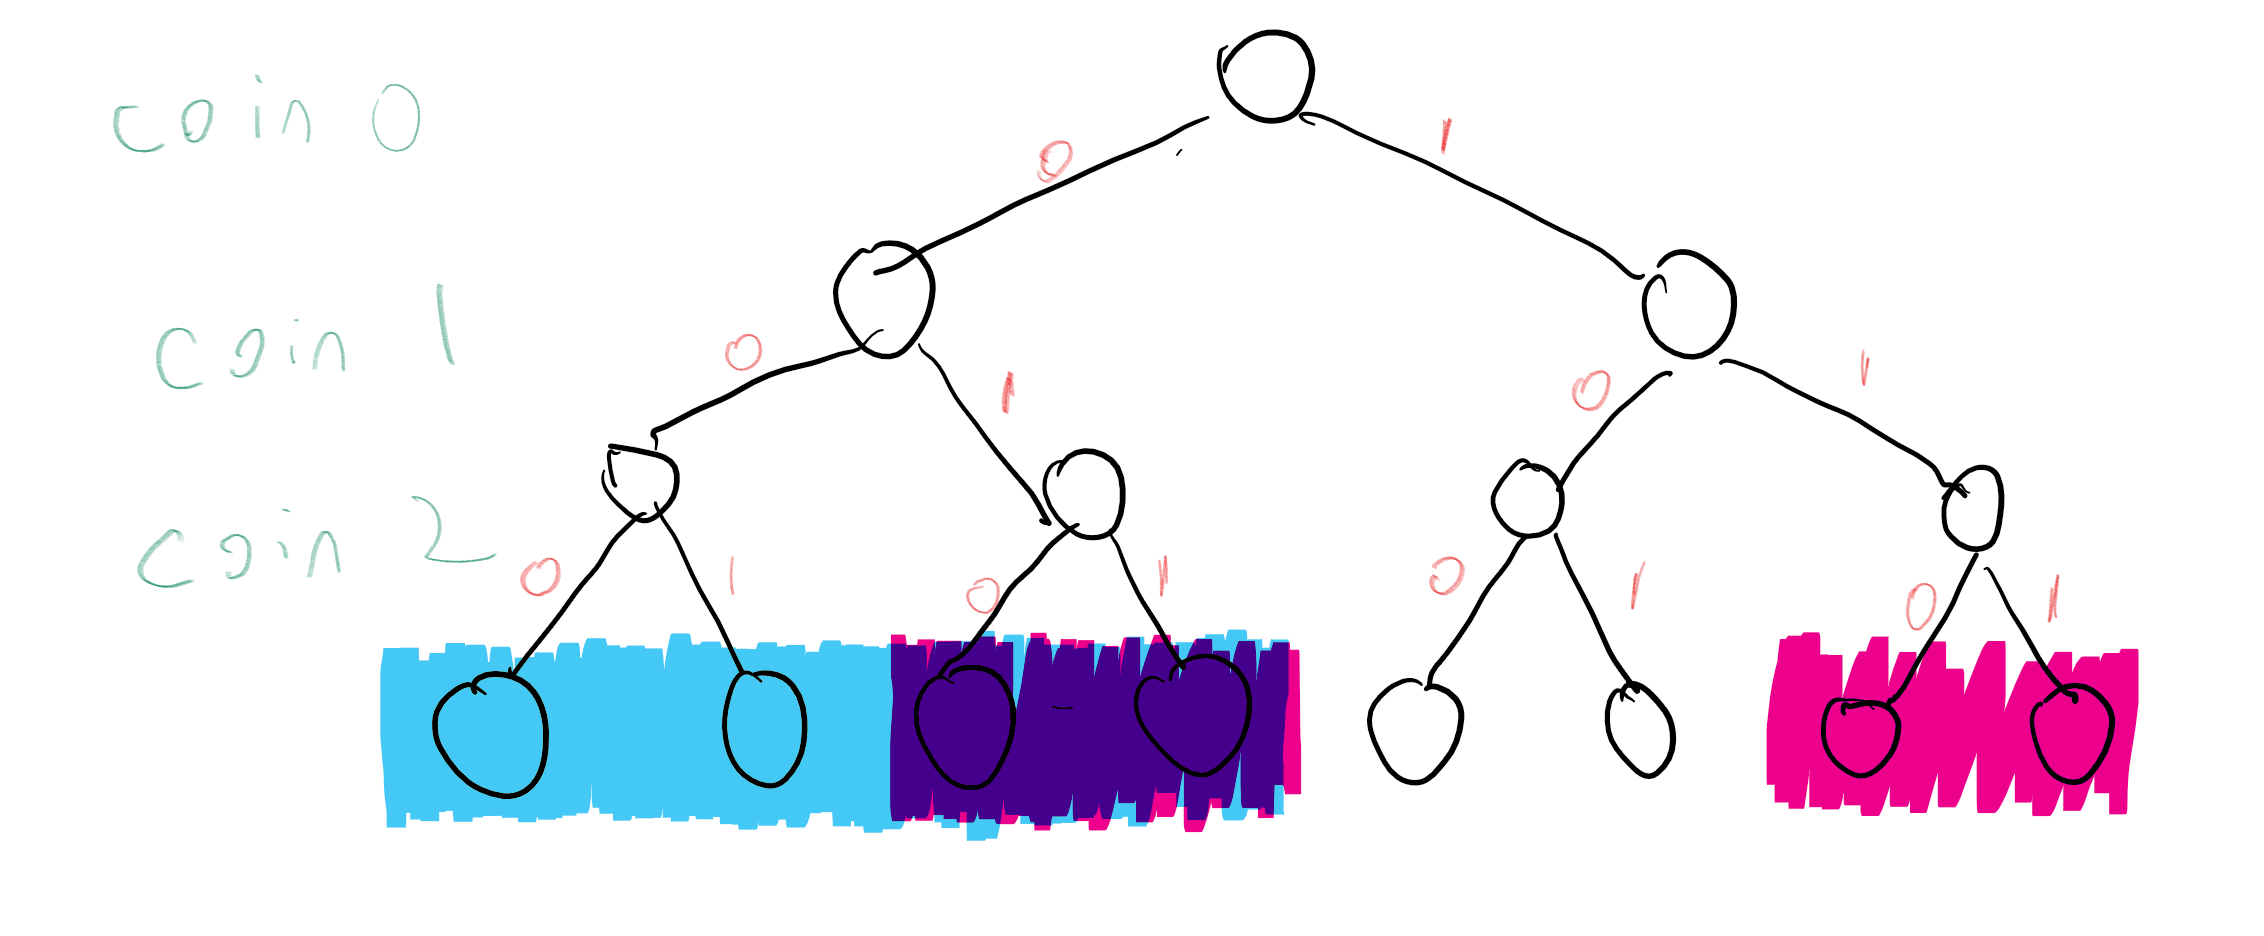
\includegraphics[width=\linewidth, height=1.5in, keepaspectratio]{../figure/coinexperiment.png}
\caption{The probabilistic experiment of tossing three coins corresponds
to making \(2\times 2 \times 2 = 8\) choices, each with equal
probability. In this example, the blue set corresponds to the event
\(A = \{ x\in \{0,1\}^3 \;|\; x_0 = 0 \}\) where the first coin toss is
equal to \(0\), and the pink set corresponds to the event
\(B = \{ x\in \{0,1\}^3 \;|\; x_1 = 1 \}\) where the second coin toss is
equal to \(1\) (with their intersection having a purplish color). As we
can see, each of these events contains \(4\) elements (out of \(8\)
total) and so has probability \(1/2\). The intersection of \(A\) and
\(B\) contains two elements, and so the probability that both of these
events occur is \(2/8 = 1/4\).}
\label{coinexperimentfig}
\end{marginfigure}

An \emph{event} is simply a subset \(A\) of \(\{0,1\}^n\). The
\emph{probability of \(A\)}, denoted by \(\Pr_{x\sim \{0,1\}^n}[A]\) (or
\(\Pr[A]\) for short, when the sample space is understood from the
context), is the probability that an \(x\) chosen uniformly at random
will be contained in \(A\). Note that this is the same as \(|A|/2^n\)
(where \(|A|\) as usual denotes the number of elements in the set
\(A\)). For example, the probability that \(x\) has an even number of
ones is \(\Pr[A]\) where
\(A=\{ x : \sum_{i=0}^{n-1} x_i \;= 0 \mod 2 \}\). In the case \(n=3\),
\(A=\{ 000,011,101,110 \}\), and hence
\(\Pr[A]=\tfrac{4}{8}=\tfrac{1}{2}\) (see \cref{eventhreecoinsfig}). It
turns out this is true for every \(n\):

\begin{marginfigure}
\centering
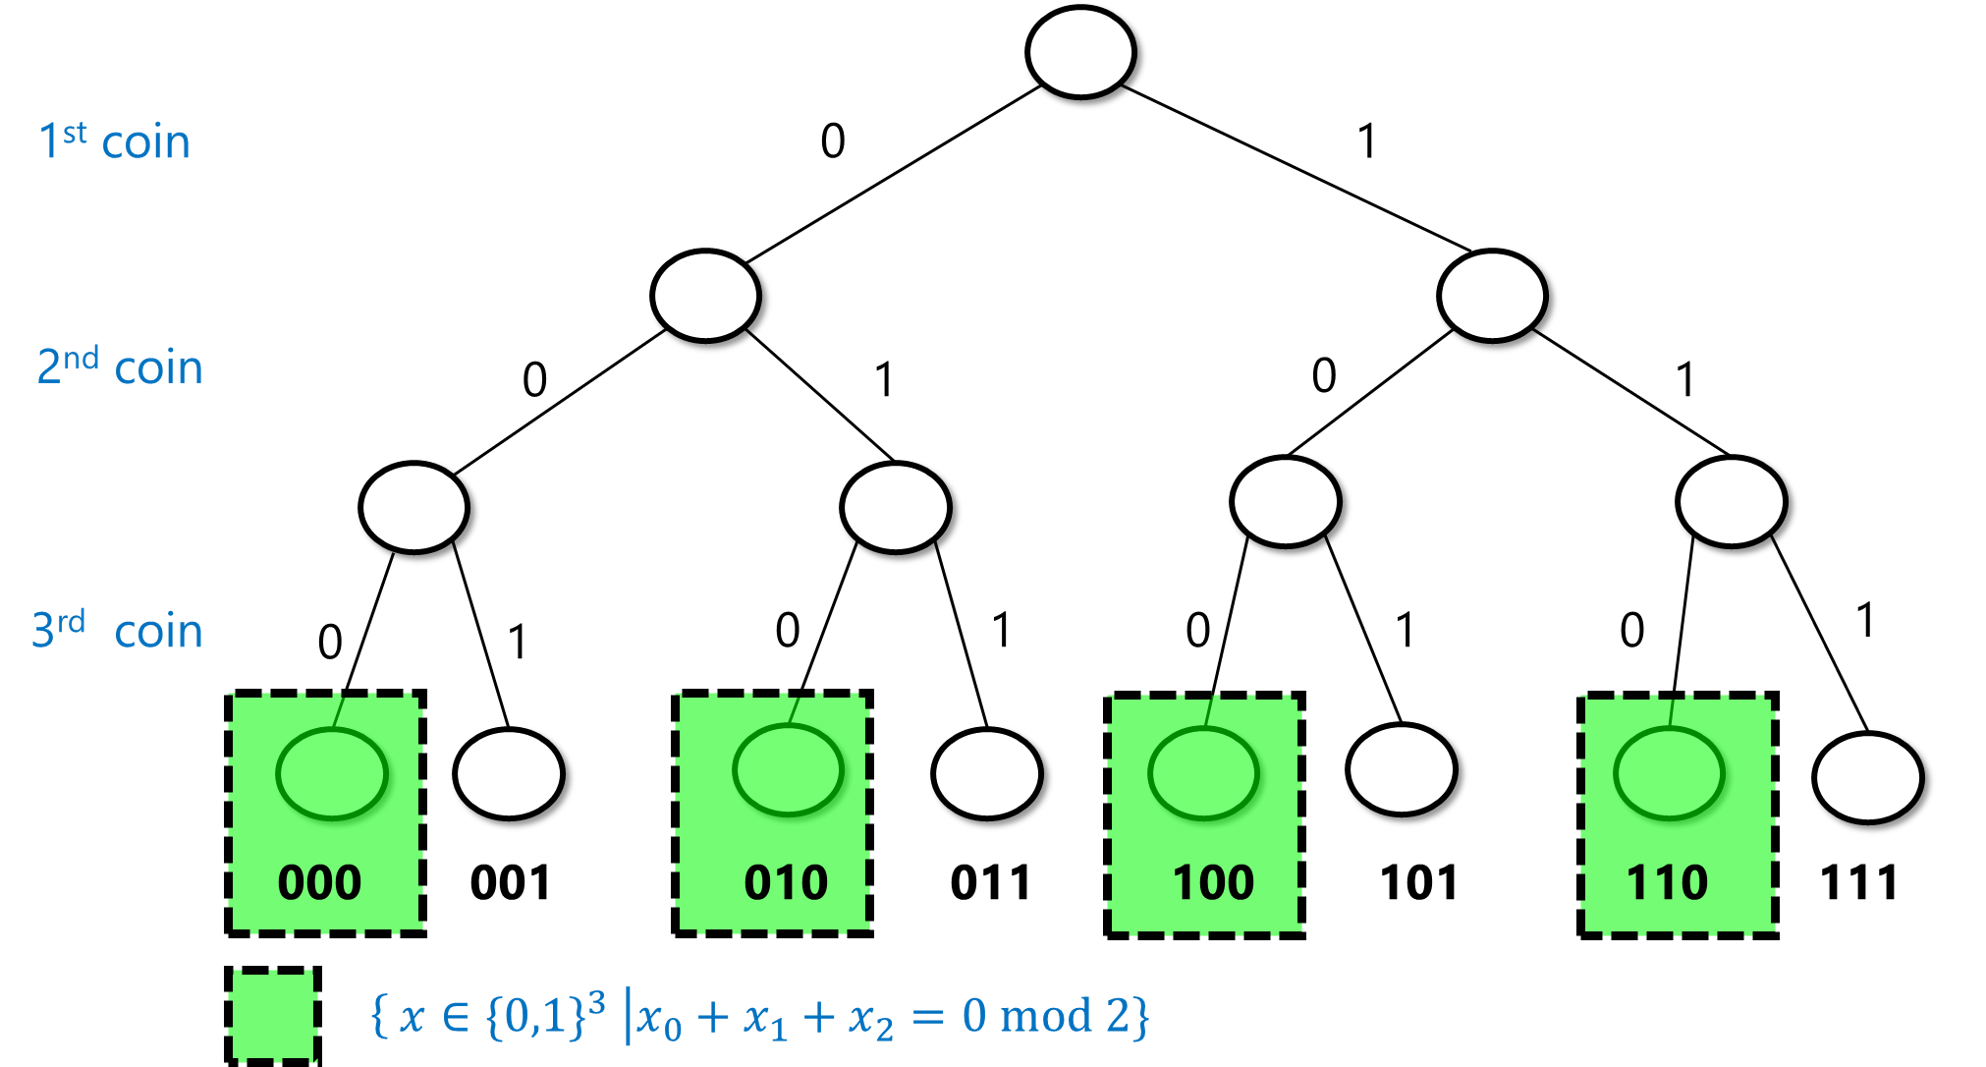
\includegraphics[width=\linewidth, height=1.5in, keepaspectratio]{../figure/even3coins.png}
\caption{The event that if we toss three coins
\(x_0,x_1,x_2 \in \{0,1\}\) then the sum of the \(x_i\)'s is even has
probability \(1/2\) since it corresponds to exactly \(4\) out of the
\(8\) possible strings of length \(3\).}
\label{eventhreecoinsfig}
\end{marginfigure}

\hypertarget{evenprob}{}
\begin{lemma} \label[lemma]{evenprob}

For every \(n>0\),
\[\Pr_{x\sim \{0,1\}^n}[ \text{$\sum_{i=0}^{n-1} x_i$ is even }] = 1/2\]

\end{lemma}

\begin{pause} \label[pause]{To-test-your-intuition-on-prob}

To test your intuition on probability, try to stop here and prove the
lemma on your own.

\end{pause}

\begin{proof}[Proof of \cref{evenprob}] \label[proof]{We-prove-the-lemma-by-inductio}

We prove the lemma by induction on \(n\). For the case \(n=1\) it is
clear since \(x=0\) is even and \(x=1\) is odd, and hence the
probability that \(x\in \{0,1\}\) is even is \(1/2\). Let \(n>1\). We
assume by induction that the lemma is true for \(n-1\) and we will prove
it for \(n\). We split the set \(\{0,1\}^n\) into four disjoint sets
\(E_0,E_1,O_0,O_1\), where for \(b\in \{0,1\}\), \(E_b\) is defined as
the set of \(x\in \{0,1\}^n\) such that \(x_0\cdots x_{n-2}\) has even
number of ones and \(x_{n-1}=b\) and similarly \(O_b\) is the set of
\(x\in \{0,1\}^n\) such that \(x_0 \cdots x_{n-2}\) has odd number of
ones and \(x_{n-1}=b\). Since \(E_0\) is obtained by simply extending
\(n-1\)-length string with even number of ones by the digit \(0\), the
size of \(E_0\) is simply the number of such \(n-1\)-length strings
which by the induction hypothesis is \(2^{n-1}/2 = 2^{n-2}\). The same
reasoning applies for \(E_1\), \(O_0\), and \(O_1\). Hence each one of
the four sets \(E_0,E_1,O_0,O_1\) is of size \(2^{n-2}\). Since
\(x\in \{0,1\}^n\) has an even number of ones if and only if
\(x \in E_0 \cup O_1\) (i.e., either the first \(n-1\) coordinates sum
up to an even number and the final coordinate is \(0\) or the first
\(n-1\) coordinates sum up to an odd number and the final coordinate is
\(1\)), we get that the probability that \(x\) satisfies this property
is \[
\tfrac{|E_0\cup O_1|}{2^n} = \frac{2^{n-2}+2^{n-2}}{2^n} = \frac{1}{2} \;,
\] using the fact that \(E_0\) and \(O_1\) are disjoint and hence
\(|E_0 \cup O_1| = |E_0|+|O_1|\).

\end{proof}

We can also use the \emph{intersection} (\(\cap\)) and \emph{union}
(\(\cup\)) operators to talk about the probability of both event \(A\)
\emph{and} event \(B\) happening, or the probability of event \(A\)
\emph{or} event \(B\) happening. For example, the probability \(p\) that
\(x\) has an \emph{even} number of ones \emph{and} \(x_0=1\) is the same
as \(\Pr[A\cap B]\) where
\(A=\{ x\in \{0,1\}^n : \sum_{i=0}^{n-1} x_i =0 \mod 2 \}\) and
\(B=\{ x\in \{0,1\}^n : x_0 = 1 \}\). This probability is equal to
\(1/4\) for \(n > 1\). (It is a great exercise for you to pause here and
verify that you understand why this is the case.)

Because intersection corresponds to considering the logical AND of the
conditions that two events happen, while union corresponds to
considering the logical OR, we will sometimes use the \(\wedge\) and
\(\vee\) operators instead of \(\cap\) and \(\cup\), and so write this
probability \(p=\Pr[A \cap B]\) defined above also as \[
\Pr_{x\sim \{0,1\}^n} \left[ \sum_i x_i =0 \mod 2 \; \wedge \; x_0 = 1 \right] \;.
\]

If \(A \subseteq \{0,1\}^n\) is an event, then
\(\overline{A} = \{0,1\}^n \setminus A\) corresponds to the event that
\(A\) does \emph{not} happen. Since \(|\overline{A}|=2^n-|A|\), we get
that
\[\Pr[\overline{A}] = \tfrac{|\overline{A}|}{2^n} = \tfrac{2^n-|A|}{2^n}=1-\tfrac{|A|}{2^n} = 1- \Pr[A]
\] This makes sense: since \(A\) happens if and only if \(\overline{A}\)
does \emph{not} happen, the probability of \(\overline{A}\) should be
one minus the probability of \(A\).

\hypertarget{samplespace}{}
\begin{remark}[Remember the sample space] \label[remark]{samplespace}

While the above definition might seem very simple and almost trivial,
the human mind seems not to have evolved for probabilistic reasoning,
and it is surprising how often people can get even the simplest settings
of probability wrong. One way to make sure you don't get confused when
trying to calculate probability statements is to always ask yourself the
following two questions: \textbf{(1)} Do I understand what is the
\textbf{sample space} that this probability is taken over?, and
\textbf{(2)} Do I understand what is the definition of the
\textbf{event} that we are analyzing?.

For example, suppose that I were to randomize seating in my course, and
then it turned out that students sitting in row 7 performed better on
the final: how surprising should we find this? If we started out with
the hypothesis that there is something special about the number 7 and
chose it ahead of time, then the event that we are discussing is the
event \(A\) that students sitting in number 7 had better performance on
the final, and we might find it surprising. However, if we first looked
at the results and then chose the row whose average performance is best,
then the event we are discussing is the event \(B\) that there exists
\emph{some} row where the performance is higher than the overall
average. \(B\) is a superset of \(A\), and its probability (even if
there is no correlation between sitting and performance) can be quite
significant.

\end{remark}

\subsection{Random variables}\label{Random-variables}

\emph{Events} correspond to Yes/No questions, but often we want to
analyze finer questions. For example, if we make a bet at the roulette
wheel, we don't want to just analyze whether we won or lost, but also
\emph{how much} we've gained. A (real valued) \emph{random variable} is
simply a way to associate a number with the result of a probabilistic
experiment. Formally, a random variable is a function
\(X:\{0,1\}^n \rightarrow \R\) that maps every outcome
\(x\in \{0,1\}^n\) to an element \(X(x) \in \R\). For example, the
function \(sum:\{0,1\}^n \rightarrow \R\) that maps \(x\) to the sum of
its coordinates (i.e., to \(\sum_{i=0}^{n-1} x_i\)) is a random
variable.

The \emph{expectation} of a random variable \(X\), denoted by \(\E[X]\),
is the average value that that this number takes, taken over all draws
from the probabilistic experiment. In other words, the expectation of
\(X\) is defined as follows: \[
\E[X] = \sum_{x\in \{0,1\}^n} 2^{-n}X(x) \;.
\]

If \(X\) and \(Y\) are random variables, then we can define \(X+Y\) as
simply the random variable that maps a point \(x\in \{0,1\}^n\) to
\(X(x)+Y(x)\). One basic and very useful property of the expectation is
that it is \emph{linear}:

\hypertarget{linearityexp}{}
\begin{lemma}[Linearity of expectation] \label[lemma]{linearityexp}

\[ \E[ X+Y ] = \E[X] + \E[Y] \]

\end{lemma}

\begin{proof} \label[proof]{begingatheredE-XY--sumxin-n-nl}

\[
\begin{gathered}
\E [X+Y] = \sum_{x\in \{0,1\}^n}2^{-n}\left(X(x)+Y(x)\right) =  \\
\sum_{x\in \{0,1\}^b} 2^{-n}X(x) + \sum_{x\in \{0,1\}^b} 2^{-n}Y(x) = \\
\E[X] + \E[Y]
\end{gathered}
\]

\end{proof}

Similarly, \(\E[kX] = k\E[X]\) for every \(k \in \R\). For example,
using the linearity of expectation, it is very easy to show that the
expectation of the sum of the \(x_i\)'s for \(x \sim \{0,1\}^n\) is
equal to \(n/2\). Indeed, if we write \(X= \sum_{i=0}^{n-1} x_i\) then
\(X= X_0 + \cdots + X_{n-1}\) where \(X_i\) is the random variable
\(x_i\). Since for every \(i\), \(\Pr[X_i=0] = 1/2\) and
\(\Pr[X_i=1]=1/2\), we get that
\(\E[X_i] = (1/2)\cdot 0 + (1/2)\cdot 1 = 1/2\) and hence
\(\E[X] = \sum_{i=0}^{n-1}\E[X_i] = n\cdot(1/2) = n/2\).

\begin{pause} \label[pause]{If-you-have-not-seen-discrete-}

If you have not seen discrete probability before, please go over this
argument again until you are sure you follow it; it is a prototypical
simple example of the type of reasoning we will employ again and again
in this course.

\end{pause}

If \(A\) is an event, then \(1_A\) is the random variable such that
\(1_A(x)\) equals \(1\) if \(x\in A\), and \(1_A(x)=0\) otherwise. Note
that \(\Pr[A] = \E[1_A]\) (can you see why?). Using this and the
linearity of expectation, we can show one of the most useful bounds in
probability theory:

\hypertarget{unionbound}{}
\begin{lemma}[Union bound] \label[lemma]{unionbound}

For every two events \(A,B\), \(\Pr[ A \cup B] \leq \Pr[A]+\Pr[B]\)

\end{lemma}

\begin{pause} \label[pause]{Before-looking-at-the-proof-tr}

Before looking at the proof, try to see why the union bound makes
intuitive sense. We can also prove it directly from the definition of
probabilities and the cardinality of sets, together with the equation
\(|A \cup B| \leq |A|+|B|\). Can you see why the latter equation is
true? (See also \cref{unionboundfig}.)

\end{pause}

\begin{proof}[Proof of \cref{unionbound}] \label[proof]{For-every-x-the-variable-Acup-}

For every \(x\), the variable \(1_{A\cup B}(x) \leq 1_A(x)+1_B(x)\).
Hence,
\(\Pr[A\cup B] = \E[ 1_{A \cup B} ] \leq \E[1_A+1_B] = \E[1_A]+\E[1_B] = \Pr[A]+\Pr[B]\).

\end{proof}

The way we often use this in theoretical computer science is to argue
that, for example, if there is a list of 100 bad events that can happen,
and each one of them happens with probability at most \(1/10000\), then
with probability at least \(1-100/10000 = 0.99\), no bad event happens.

\begin{marginfigure}
\centering
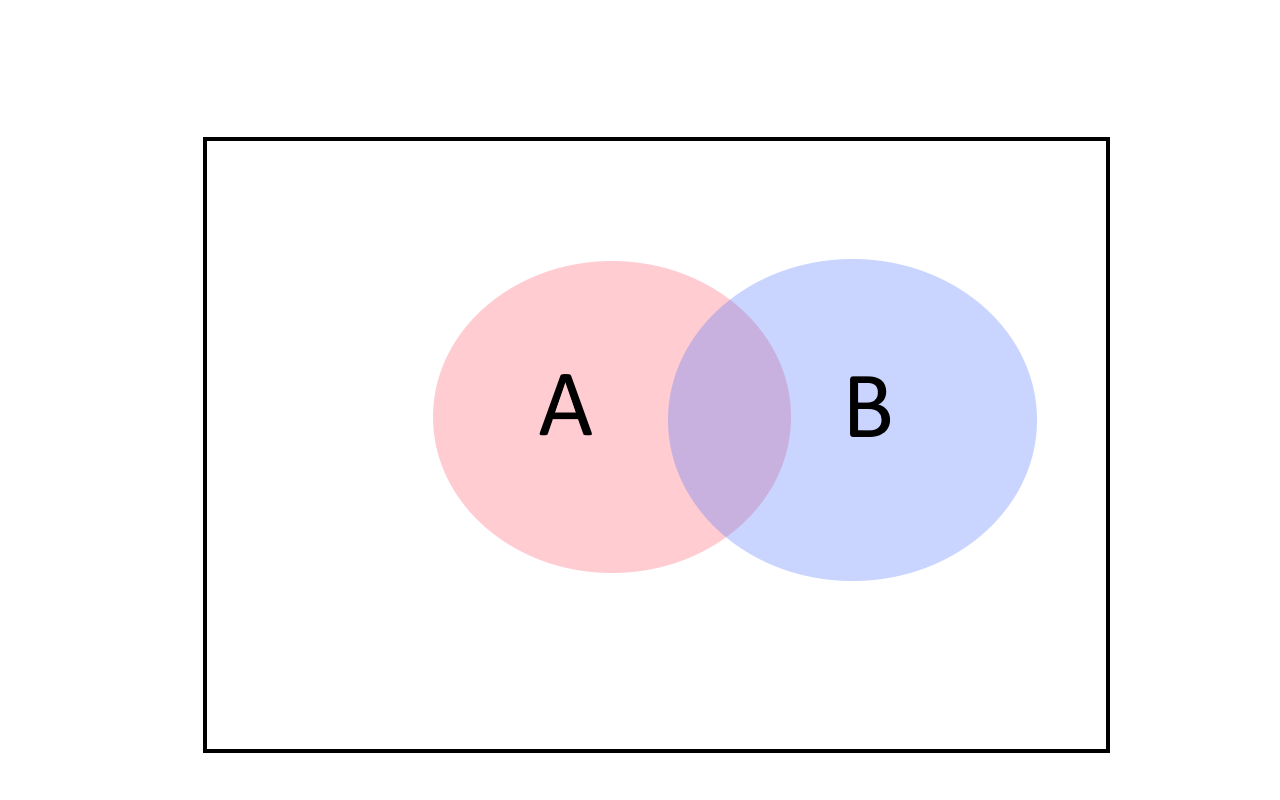
\includegraphics[width=\linewidth, height=1.5in, keepaspectratio]{../figure/unionbound.png}
\caption{The \emph{union bound} tells us that the probability of \(A\)
or \(B\) happening is at most the sum of the individual probabilities.
We can see it by noting that for every two sets
\(|A\cup B| \leq |A|+|B|\) (with equality only if \(A\) and \(B\) have
no intersection).}
\label{unionboundfig}
\end{marginfigure}

\subsection{Distributions over
strings}\label{Distributions-over-strings}

While most of the time we think of random variables as having as output
a \emph{real number}, we sometimes consider random variables whose
output is a \emph{string}. That is, we can think of a map
\(Y:\{0,1\}^n \rightarrow \{0,1\}^*\) and consider the ``random
variable'' \(Y\) such that for every \(y\in \{0,1\}^*\), the probability
that \(Y\) outputs \(y\) is equal to
\(\tfrac{1}{2^n}\left| \{ x \in \{0,1\}^n \;|\; Y(x)=y \}\right|\). To
avoid confusion, we will typically refer to such string-valued random
variables as \emph{distributions} over strings. So, a
\emph{distribution} \(Y\) over strings \(\{0,1\}^*\) can be thought of
as a finite collection of strings \(y_0,\ldots,y_{M-1} \in \{0,1\}^*\)
and probabilities \(p_0,\ldots,p_{M-1}\) (which are non-negative numbers
summing up to one), so that \(\Pr[ Y = y_i ] = p_i\).

Two distributions \(Y\) and \(Y'\) are \emph{identical} if they assign
the same probability to every string. For example, consider the
following two functions \(Y,Y':\{0,1\}^2 \rightarrow \{0,1\}^2\). For
every \(x \in \{0,1\}^2\), we define \(Y(x)=x\) and
\(Y'(x)=x_0(x_0\oplus x_1)\) where \(\oplus\) is the XOR operations.
Although these are two different functions, they induce the same
distribution over \(\{0,1\}^2\) when invoked on a uniform input. The
distribution \(Y(x)\) for \(x\sim \{0,1\}^2\) is of course the uniform
distribution over \(\{0,1\}^2\). On the other hand \(Y'\) is simply the
map \(00 \mapsto 00\), \(01 \mapsto 01\), \(10 \mapsto 11\),
\(11 \mapsto 10\) which is a permutation over the map
\(F:\{0,1\}^2 \rightarrow \{0,1\}^2\) defined as \(F(x_0x_1)=x_0x_1\)
and the map \(G:\{0,1\}^2 \rightarrow \{0,1\}^2\) defined as
\(G(x_0x_1)=x_0(x_0 \oplus x_1)\)

\subsection{More general sample
spaces.}\label{More-general-sample-spaces}

While in this chapter we assume that the underlying probabilistic
experiment corresponds to tossing \(n\) independent coins, everything we
say easily generalizes to sampling \(x\) from a more general finite or
countable set \(S\) (and not-so-easily generalizes to uncountable sets
\(S\) as well). A \emph{probability distribution} over a finite set
\(S\) is simply a function \(\mu : S \rightarrow [0,1]\) such that
\(\sum_{x\in S}\mu(s)=1\). We think of this as the experiment where we
obtain every \(x\in S\) with probability \(\mu(s)\), and sometimes
denote this as \(x\sim \mu\). An \emph{event} \(A\) is a subset of
\(S\), and the probability of \(A\), which we denote by \(\Pr_\mu[A]\),
is \(\sum_{x\in A} \mu(x)\). A \emph{random variable} is a function
\(X:S \rightarrow \R\), where the probability that \(X=y\) is equal to
\(\sum_{x\in S \text{ s.t. } X(x)=y} \mu(x)\).

\section{Correlations and
independence}\label{Correlations-and-independence}

One of the most delicate but important concepts in probability is the
notion of \emph{independence} (and the opposing notion of
\emph{correlations}). Subtle correlations are often behind surprises and
errors in probability and statistical analysis, and several mistaken
predictions have been blamed on miscalculating the correlations between,
say, housing prices in Florida and Arizona, or voter preferences in Ohio
and Michigan. See also Joe Blitzstein's aptly named talk
\href{https://youtu.be/dzFf3r1yph8}{``Conditioning is the Soul of
Statistics''}. (Another thorny issue is of course the difference between
\emph{correlation} and \emph{causation}. Luckily, this is another point
we don't need to worry about in our clean setting of tossing \(n\)
coins.)

Two events \(A\) and \(B\) are \emph{independent} if the fact that \(A\)
happens makes \(B\) neither more nor less likely to happen. For example,
if we think of the experiment of tossing \(3\) random coins
\(x\in \{0,1\}^3\), and we let \(A\) be the event that \(x_0=1\) and
\(B\) the event that \(x_0 + x_1 + x_2 \geq 2\), then if \(A\) happens
it is more likely that \(B\) happens, and hence these events are
\emph{not} independent. On the other hand, if we let \(C\) be the event
that \(x_1=1\), then because the second coin toss is not affected by the
result of the first one, the events \(A\) and \(C\) are independent.

The formal definition is that events \(A\) and \(B\) are
\emph{independent} if \(\Pr[A \cap B]=\Pr[A] \cdot \Pr[B]\). If
\(\Pr[A \cap B] > \Pr[A]\cdot \Pr[B]\) then we say that \(A\) and \(B\)
are \emph{positively correlated}, while if
\(\Pr[ A \cap B] < \Pr[A] \cdot \Pr[B]\) then we say that \(A\) and
\(B\) are \emph{negatively correlated} (see \cref{coinexperimentfig}).

\begin{marginfigure}
\centering
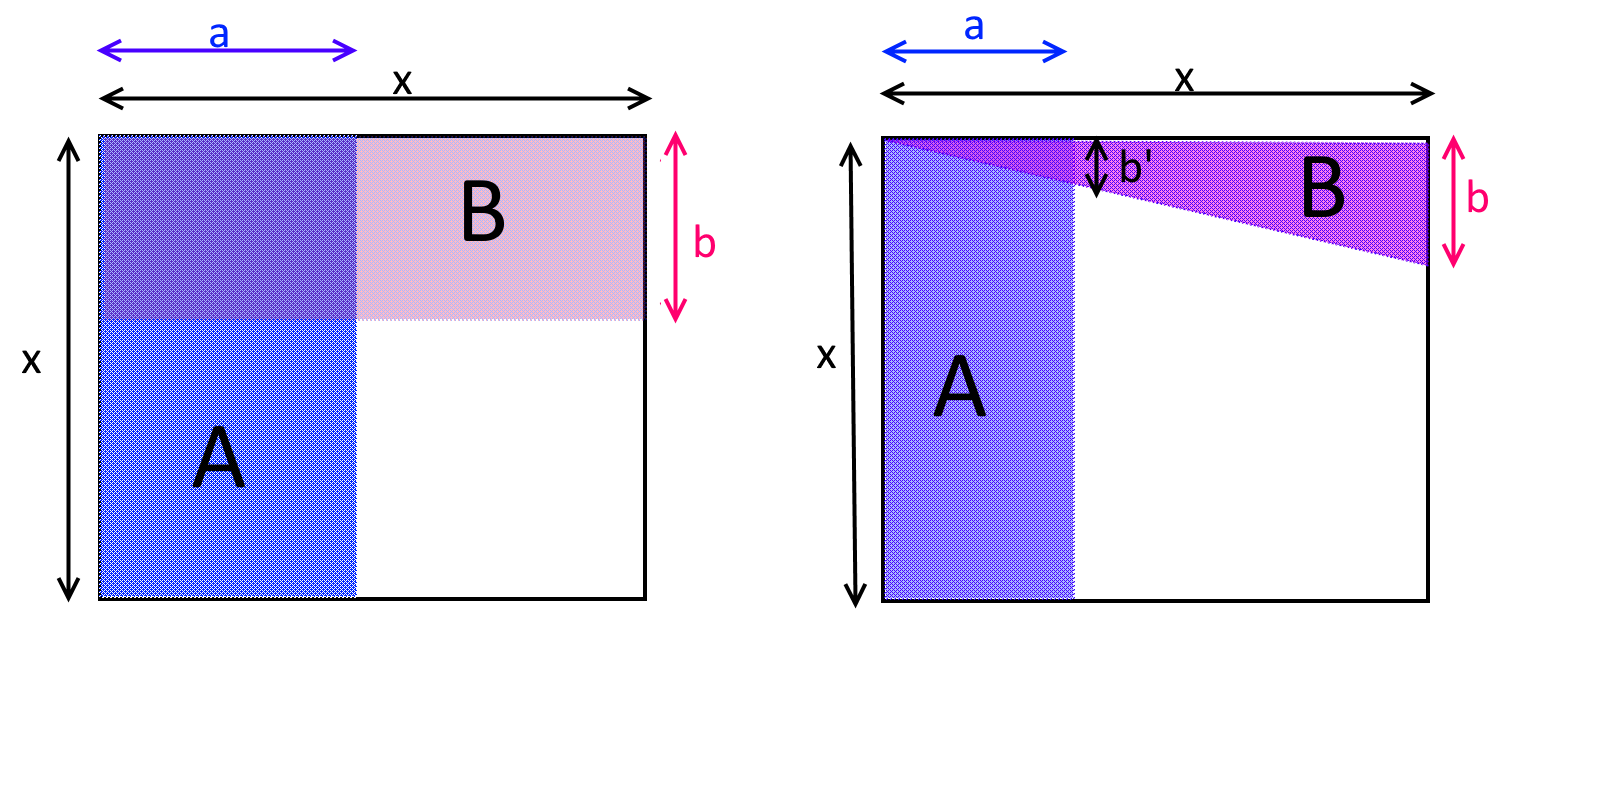
\includegraphics[width=\linewidth, height=1.5in, keepaspectratio]{../figure/independence.png}
\caption{Two events \(A\) and \(B\) are \emph{independent} if
\(\Pr[A \cap B]=\Pr[A]\cdot \Pr[B]\). In the two figures above, the
empty \(x\times x\) square is the sample space, and \(A\) and \(B\) are
two events in this sample space. In the left figure, \(A\) and \(B\) are
independent, while in the right figure they are negatively correlated,
since \(B\) is less likely to occur if we condition on \(A\) (and vice
versa). Mathematically, one can see this by noticing that in the left
figure the areas of \(A\) and \(B\) respectively are \(a\cdot x\) and
\(b\cdot x\), and so their probabilities are
\(\tfrac{a\cdot x}{x^2}=\tfrac{a}{x}\) and
\(\tfrac{b\cdot x}{x^2}=\tfrac{b}{x}\) respectively, while the area of
\(A \cap B\) is \(a\cdot b\) which corresponds to the probability
\(\tfrac{a\cdot b}{x^2}\). In the right figure, the area of the triangle
\(B\) is \(\tfrac{b\cdot x}{2}\) which corresponds to a probability of
\(\tfrac{b}{2x}\), but the area of \(A \cap B\) is
\(\tfrac{b' \cdot a}{2}\) for some \(b'<b\). This means that the
probability of \(A \cap B\) is
\(\tfrac{b'\cdot a}{2x^2} < \tfrac{b}{2x} \cdot \tfrac{a}{x}\), or in
other words \(\Pr[A \cap B ] < \Pr[A] \cdot \Pr[B]\).}
\label{independencefig}
\end{marginfigure}

If we consider the above examples on the experiment of choosing
\(x\in \{0,1\}^3\) then we can see that

\[
\begin{aligned}
\Pr[x_0=1] &= \tfrac{1}{2} \\
\Pr[x_0+x_1+x_2 \geq 2] = \Pr[\{ 011,101,110,111 \}] &= \tfrac{4}{8} = \tfrac{1}{2}
\end{aligned}
\]

but

\[
\Pr[x_0 =1 \; \wedge \; x_0+x_1+x_2 \geq 2 ] = \Pr[ \{101,110,111 \} ] = \tfrac{3}{8} > \tfrac{1}{2} \cdot \tfrac{1}{2}
\]

and hence, as we already observed, the events \(\{ x_0 = 1 \}\) and
\(\{ x_0+x_1+x_2 \geq 2 \}\) are not independent and in fact are
positively correlated. On the other hand,
\(\Pr[ x_0 = 1 \wedge x_1 = 1 ] = \Pr[ \{110,111 \}] = \tfrac{2}{8} = \tfrac{1}{2} \cdot \tfrac{1}{2}\)
and hence the events \(\{x_0 = 1 \}\) and \(\{ x_1 = 1 \}\) are indeed
independent.

\hypertarget{disjoint}{}
\begin{remark}[Disjointness vs independence] \label[remark]{disjoint}

People sometimes confuse the notion of \emph{disjointness} and
\emph{independence}, but these are actually quite different. Two events
\(A\) and \(B\) are \emph{disjoint} if \(A \cap B = \emptyset\), which
means that if \(A\) happens then \(B\) definitely does not happen. They
are \emph{independent} if \(\Pr[A \cap B]=\Pr[A]\Pr[B]\) which means
that knowing that \(A\) happens gives us no information about whether
\(B\) happened or not. If \(A\) and \(B\) have nonzero probability, then
being disjoint implies that they are \emph{not} independent, since in
particular it means that they are negatively correlated.

\end{remark}

\paragraph{Conditional probability:} If \(A\) and \(B\) are events, and
\(A\) happens with nonzero probability then we define the probability
that \(B\) happens \emph{conditioned on \(A\)} to be
\(\Pr[B|A] = \Pr[A \cap B]/\Pr[A]\). This corresponds to calculating the
probability that \(B\) happens if we already know that \(A\) happened.
Note that \(A\) and \(B\) are independent if and only if
\(\Pr[B|A]=\Pr[B]\).

\paragraph{More than two events:} We can generalize this definition to
more than two events. We say that events \(A_1,\ldots,A_k\) are
\emph{mutually independent} if knowing that any set of them occurred or
didn't occur does not change the probability that an event outside the
set occurs. Formally, the condition is that for every subset
\(I \subseteq [k]\), \[
\Pr[ \wedge_{i\in I} A_i] =\prod_{i\in I} \Pr[A_i].
\]

For example, if \(x\sim \{0,1\}^3\), then the events \(\{ x_0=1 \}\),
\(\{ x_1 = 1\}\) and \(\{x_2 = 1 \}\) are mutually independent. On the
other hand, the events \(\{x_0 = 1 \}\), \(\{x_1 = 1\}\) and
\(\{ x_0 + x_1 = 0 \mod 2 \}\) are \emph{not} mutually independent, even
though every pair of these events is independent (can you see why? see
also \cref{independencecoinsfig}).

\begin{marginfigure}
\centering
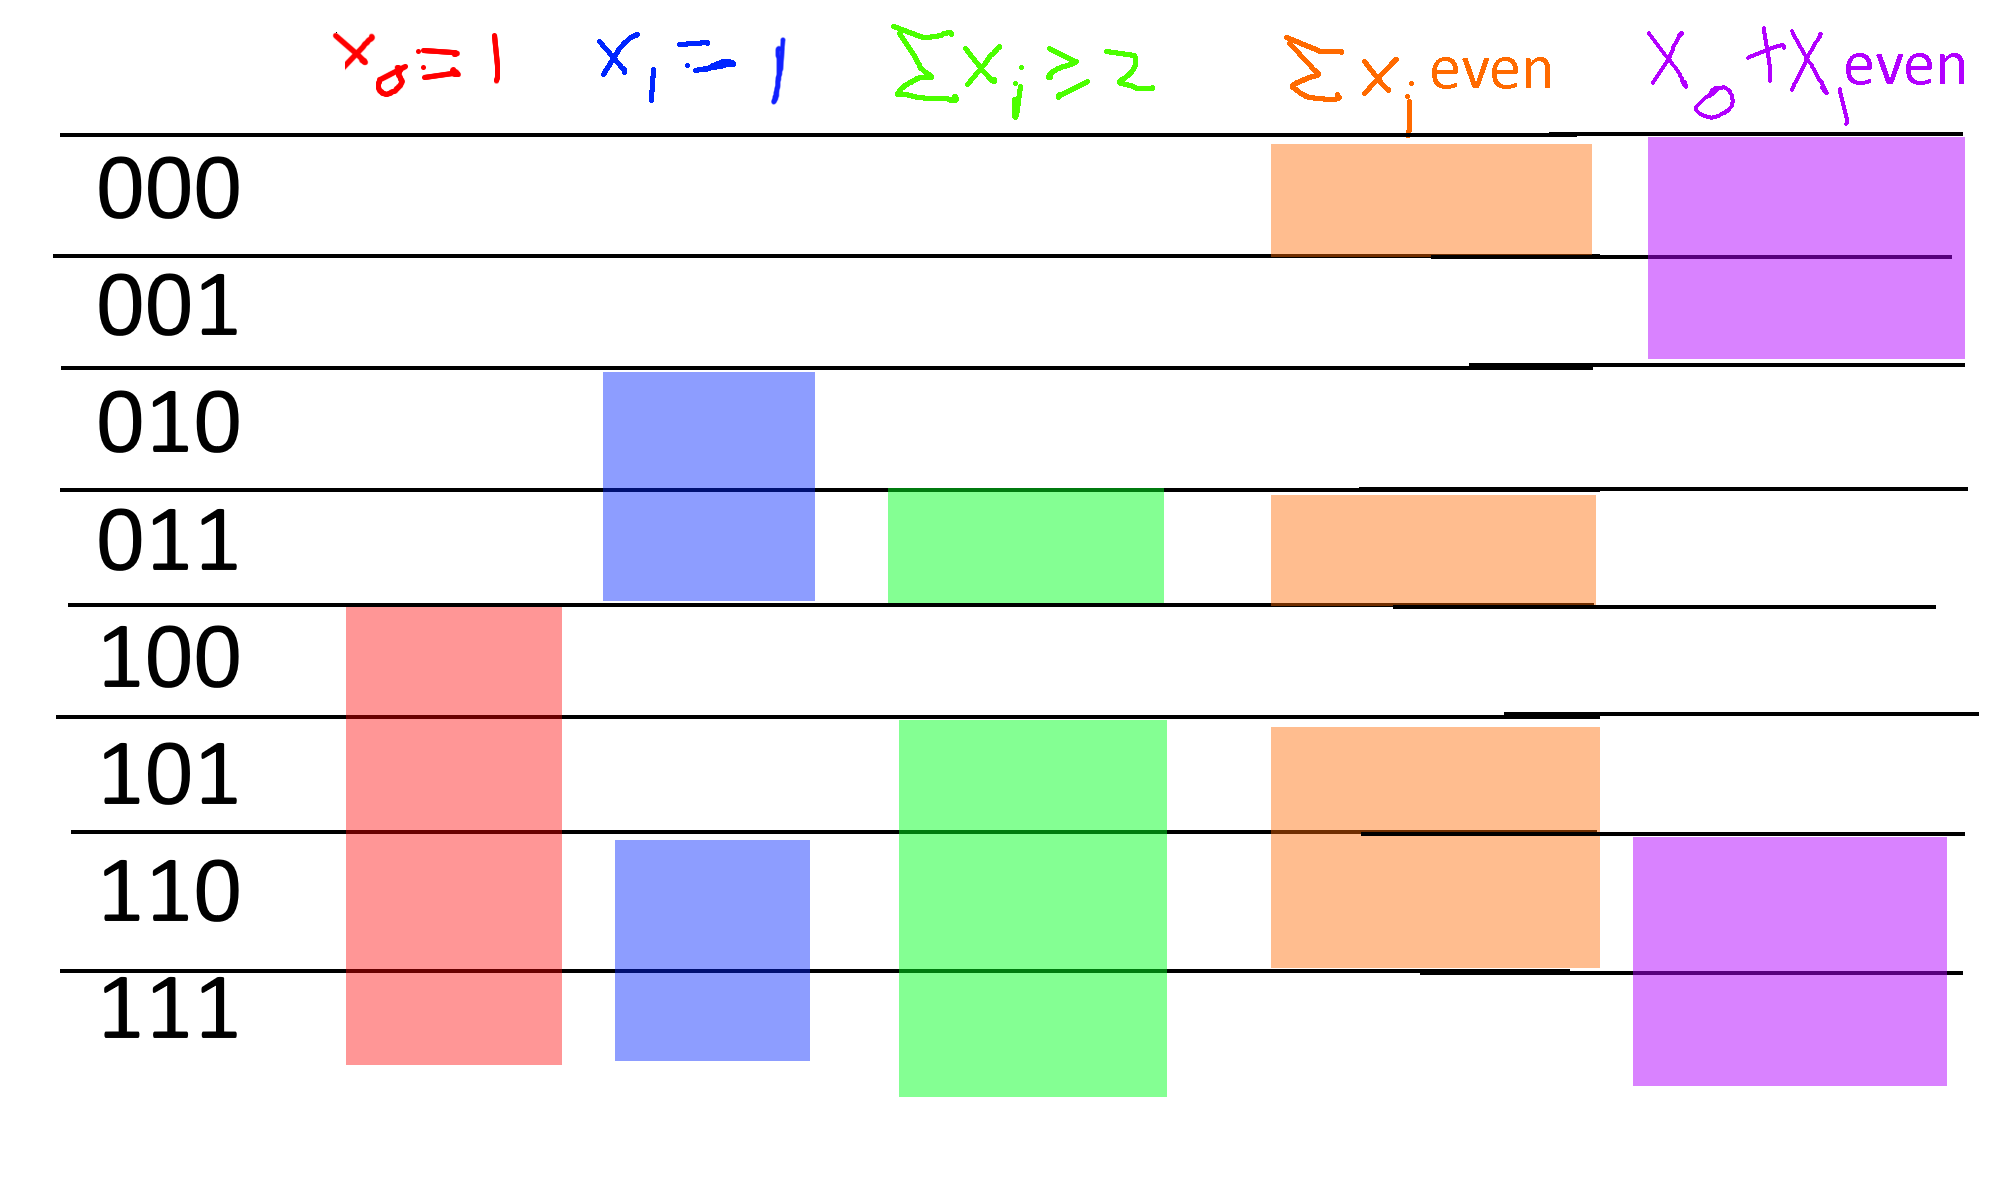
\includegraphics[width=\linewidth, height=1.5in, keepaspectratio]{../figure/independencecoins.png}
\caption{Consider the sample space \(\{0,1\}^n\) and the events
\(A,B,C,D,E\) corresponding to \(A\): \(x_0=1\), \(B\): \(x_1=1\),
\(C\): \(x_0+x_1+x_2 \geq 2\), \(D\): \(x_0+x_1+x_2 = 0 mod 2\) and
\(D\): \(x_0+x_1 = 0 mod 2\). We can see that \(A\) and \(B\) are
independent, \(C\) is positively correlated with \(A\) and positively
correlated with \(B\), the three events \(A,B,D\) are mutually
independent, and while every pair out of \(A,B,E\) is independent, the
three events \(A,B,E\) are not mutually independent since their
intersection has probability \(\tfrac{2}{8}=\tfrac{1}{4}\) instead of
\(\tfrac{1}{2}\cdot \tfrac{1}{2} \cdot \tfrac{1}{2} = \tfrac{1}{8}\).}
\label{independencecoinsfig}
\end{marginfigure}

\subsection{Independent random
variables}\label{Independent-random-variables}

We say that two random variables \(X:\{0,1\}^n \rightarrow \R\) and
\(Y:\{0,1\}^n \rightarrow \R\) are independent if for every
\(u,v \in \R\), the events \(\{ X=u \}\) and \(\{ Y=v \}\) are
independent. (We use \(\{ X=u \}\) as shorthand for
\(\{ x \;|\; X(x)=u \}\).) In other words, \(X\) and \(Y\) are
independent if \(\Pr[ X=u \wedge Y=v]=\Pr[X=u]\Pr[Y=v]\) for every
\(u,v \in \R\). For example, if two random variables depend on the
result of tossing different coins then they are independent:

\hypertarget{indcoins}{}
\begin{lemma} \label[lemma]{indcoins}

Suppose that \(S=\{ s_0,\ldots, s_{k-1} \}\) and
\(T=\{ t_0 ,\ldots, t_{m-1} \}\) are disjoint subsets of
\(\{0,\ldots,n-1\}\) and let \(X,Y:\{0,1\}^n \rightarrow \R\) be random
variables such that \(X=F(x_{s_0},\ldots,x_{s_{k-1}})\) and
\(Y=G(x_{t_0},\ldots,x_{t_{m-1}})\) for some functions
\(F: \{0,1\}^k \rightarrow \R\) and \(G: \{0,1\}^m \rightarrow \R\).
Then \(X\) and \(Y\) are independent.

\end{lemma}

\begin{pause} \label[pause]{The-notation-in-the-lemmas-sta}

The notation in the lemma's statement is a bit cumbersome, but at the
end of the day, it simply says that if \(X\) and \(Y\) are random
variables that depend on two disjoint sets \(S\) and \(T\) of coins (for
example, \(X\) might be the sum of the first \(n/2\) coins, and \(Y\)
might be the largest consecutive stretch of zeroes in the second \(n/2\)
coins), then they are independent.

\end{pause}

\begin{proof}[Proof of \cref{indcoins}] \label[proof]{Let-abin-R-and-let-A---x-in-k-}

Let \(a,b\in \R\), and let \(A = \{ x \in \{0,1\}^k : F(x)=a \}\) and
\(B=\{ x\in \{0,1\}^m : F(x)=b \}\). Since \(S\) and \(T\) are disjoint,
we can reorder the indices so that \(S = \{0,\ldots,k-1\}\) and
\(T=\{k,\ldots,k+m-1\}\) without affecting any of the probabilities.
Hence we can write \(\Pr[X=a \wedge X=b] = |C|/2^n\) where
\(C= \{ x_0,\ldots,x_{n-1} : (x_0,\ldots,x_{k-1}) \in A \wedge (x_k,\ldots,x_{k+m-1}) \in B \}\).
Another way to write this using string concatenation is that
\(C = \{ xyz : x\in A, y\in B, z\in \{0,1\}^{n-k-m} \}\), and hence
\(|C|=|A||B|2^{n-k-m}\), which means that \[
\tfrac{|C|}{2^n} = \tfrac{|A|}{2^k}\tfrac{|B|}{2^m}\tfrac{2^{n-k-m}}{2^{n-k-m}}=\Pr[X=a]\Pr[Y=b] .
\]

\end{proof}

Note that if \(X\) and \(Y\) are independent random variables then (if
we let \(S_X,S_Y\) denote all the numbers that have positive probability
of being the output of \(X\) and \(Y\), respectively) it holds that: \[
\begin{gathered}
\E[ \ensuremath{\mathit{XY}} ] = \sum_{a \in S_X,b \in S_Y} {\textstyle\Pr[X=a \wedge Y=b]}\cdot ab \; =^{(1)} \; \sum_{a \in S_X,b \in S_Y} {\textstyle \Pr[X=a]\Pr[Y=b]}\cdot ab =^{(2)} \\
\left(\sum_{a \in S_X} {\textstyle \Pr[X=a]}\cdot a\right)\left(\sum_{b \in S_Y} {\textstyle \Pr[Y=b]}b\right) =^{(3)} \\
\E[X] \E[Y]
\end{gathered}
\] where the first equality (\(=^{(1)}\)) follows from the independence
of \(X\) and \(Y\), the second equality (\(=^{(2)}\)) follows by
``opening the parentheses'' of the righthand side, and the third
inequality (\(=^{(3)}\)) follows from the definition of expectation.
(This is not an ``if and only if''; see \cref{noindnocorex}.)

Another useful fact is that if \(X\) and \(Y\) are independent random
variables, then so are \(F(X)\) and \(G(Y)\) for all functions
\(F,G:\R \rightarrow R\). This is intuitively true since learning
\(F(X)\) can only provide us with less information than does learning
\(X\) itself. Hence, if learning \(X\) does not teach us anything about
\(Y\) (and so also about \(F(Y)\)) then neither will learning \(F(X)\).
Indeed, to prove this we can write for every \(a,b \in \R\):

\[
\begin{gathered}
\Pr[ F(X)=a \wedge G(Y)=b ] = \sum_{x \text{ s.t.} F(x)=a, y \text{ s.t. } G(y)=b} \Pr[ X=x \wedge Y=y ] = \\
\sum_{x \text{ s.t.} F(x)=a, y \text{ s.t. } G(y)=b} \Pr[ X=x ] \Pr[  Y=y ]  = \\
\left( \sum_{x \text{ s.t.} F(x)=a } \Pr[X=x ] \right) \cdot \left( \sum_{y \text{ s.t.} G(y)=b } \Pr[Y=y ] \right) = \\
\Pr[ F(X)=a] \Pr[G(Y)=b] .
\end{gathered}
\]

\subsection{Collections of independent random
variables.}\label{Collections-of-independent-ran}

We can extend the notions of independence to more than two random
variables: we say that the random variables \(X_0,\ldots,X_{n-1}\) are
\emph{mutually independent} if for every \(a_0,\ldots,a_{n-1} \in \R\),
\[
\Pr\left[X_0=a_0 \wedge \cdots \wedge X_{n-1}=a_{n-1}\right]=\Pr[X_0=a_0]\cdots \Pr[X_{n-1}=a_{n-1}] .
\] And similarly, we have that

\hypertarget{expprod}{}
\begin{lemma}[Expectation of product of independent random variables] \label[lemma]{expprod}

If \(X_0,\ldots,X_{n-1}\) are mutually independent then \[
\E[ \prod_{i=0}^{n-1} X_i ] = \prod_{i=0}^{n-1} \E[X_i] .
\]

\end{lemma}

\hypertarget{indeplem}{}
\begin{lemma}[Functions preserve independence] \label[lemma]{indeplem}

If \(X_0,\ldots,X_{n-1}\) are mutually independent, and
\(Y_0,\ldots,Y_{n-1}\) are defined as \(Y_i = F_i(X_i)\) for some
functions \(F_0,\ldots,F_{n-1}:\R \rightarrow \R\), then
\(Y_0,\ldots,Y_{n-1}\) are mutually independent as well.

\end{lemma}

\begin{pause} \label[pause]{We-leave-proving-crefexpprod-a}

We leave proving \cref{expprod} and \cref{indeplem} as \cref{expprodex}
\cref{indeplemex}. It is good idea for you stop now and do these
exercises to make sure you are comfortable with the notion of
independence, as we will use it heavily later on in this course.

\end{pause}

\section{Concentration and tail
bounds}\label{Concentration-and-tail-bounds}

The name ``expectation'' is somewhat misleading. For example, suppose
that you and I place a bet on the outcome of 10 coin tosses, where if
they all come out to be \(1\)'s then I pay you 100,000 dollars and
otherwise you pay me 10 dollars. If we let
\(X:\{0,1\}^{10} \rightarrow \R\) be the random variable denoting your
gain, then we see that

\[
\E[X] = 2^{-10}\cdot 100000 - (1-2^{-10})10 \sim 90 .
\]

But we don't really ``expect'' the result of this experiment to be for
you to gain 90 dollars. Rather, 99.9\% of the time you will pay me 10
dollars, and you will hit the jackpot 0.01\% of the times.

However, if we repeat this experiment again and again (with fresh and
hence \emph{independent} coins), then in the long run we do expect your
average earning to be close to 90 dollars, which is the reason why
casinos can make money in a predictable way even though every individual
bet is random. For example, if we toss \(n\) independent and unbiased
coins, then as \(n\) grows, the number of coins that come up ones will
be more and more \emph{concentrated} around \(n/2\) according to the
famous ``bell curve'' (see \cref{bellfig}).

\begin{marginfigure}
\centering
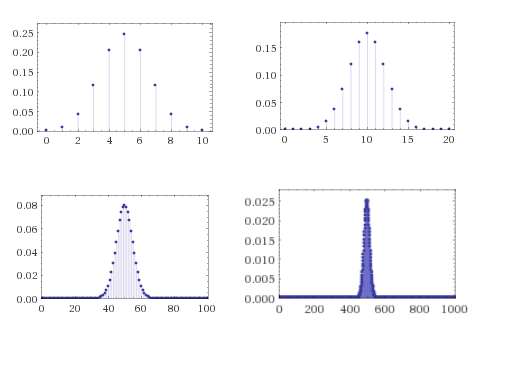
\includegraphics[width=\linewidth, height=1.5in, keepaspectratio]{../figure/binomial.png}
\caption{The probabilities that we obtain a particular sum when we toss
\(n=10,20,100,1000\) coins converge quickly to the Gaussian/normal
distribution.}
\label{bellfig}
\end{marginfigure}

Much of probability theory is concerned with so called
\emph{concentration} or \emph{tail} bounds, which are upper bounds on
the probability that a random variable \(X\) deviates too much from its
expectation. The first and simplest one of them is Markov's inequality:

\hypertarget{markovthm}{}
\begin{theorem}[Markov's inequality] \label[theorem]{markovthm}

If \(X\) is a non-negative random variable then
\(\Pr[ X \geq k \E[X] ] \leq 1/k\).

\end{theorem}

\begin{pause} \label[pause]{Markovs-Inequality-is-actually}

Markov's Inequality is actually a very natural statement (see also
\cref{markovfig}). For example, if you know that the average (not the
median!) household income in the US is 70,000 dollars, then in
particular you can deduce that at most 25 percent of households make
more than 280,000 dollars, since otherwise, even if the remaining 75
percent had zero income, the top 25 percent alone would cause the
average income to be larger than 70,000 dollars. From this example you
can already see that in many situations, Markov's inequality will not be
\emph{tight} and the probability of deviating from expectation will be
much smaller: see the Chebyshev and Chernoff inequalities below.

\end{pause}

\begin{proof}[Proof of \cref{markovthm}] \label[proof]{Let-mu--EX-and-define-YX-geq-k}

Let \(\mu = \E[X]\) and define \(Y=1_{X \geq k \mu}\). That is,
\(Y(x)=1\) if \(X(x) \geq k \mu\) and \(Y(x)=0\) otherwise. Note that by
definition, for every \(x\), \(Y(x) \leq X/(k\mu)\). We need to show
\(\E[Y] \leq 1/k\). But this follows since
\(\E[Y] \leq \E[X/k(\mu)] = \E[X]/(k\mu) = \mu/(k\mu)=1/k\).

\end{proof}

\begin{marginfigure}
\centering
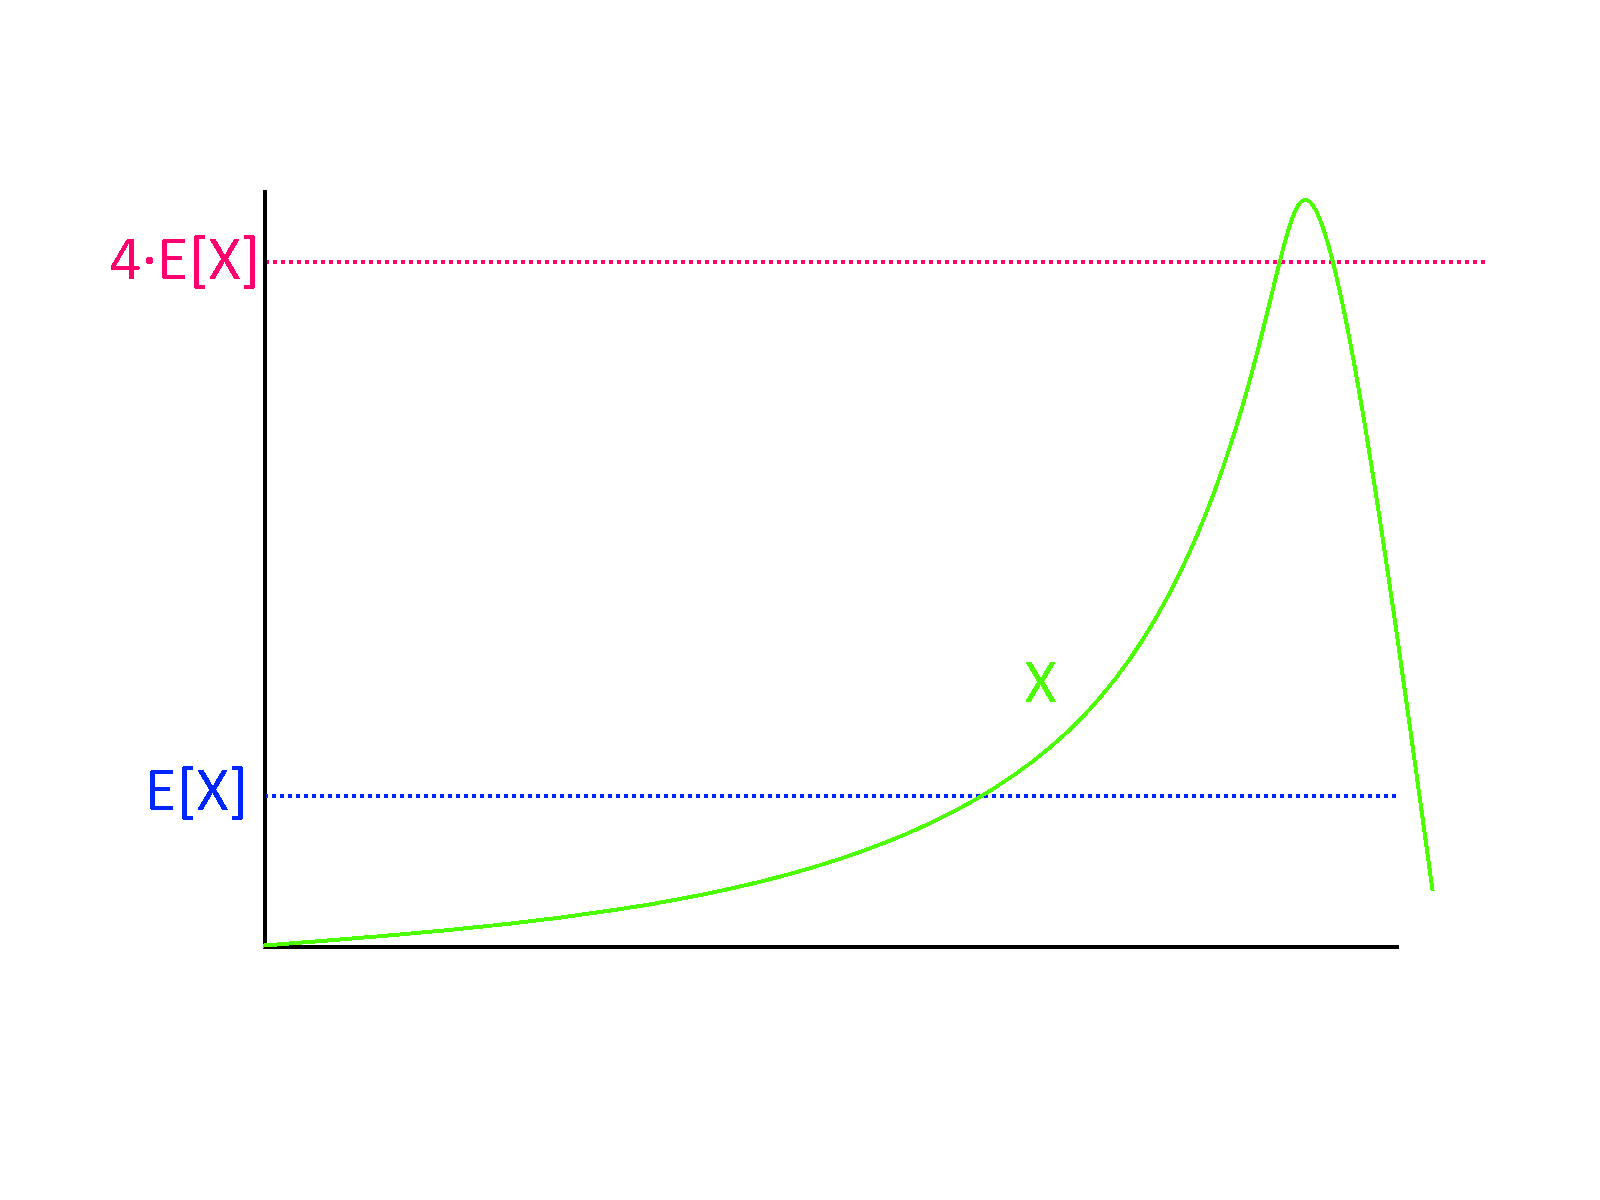
\includegraphics[width=\linewidth, height=1.5in, keepaspectratio]{../figure/markovineq.png}
\caption{Markov's Inequality tells us that a non-negative random
variable \(X\) cannot be much larger than its expectation, with high
probability. For example, if the expectation of \(X\) is \(\mu\), then
the probability that \(X>4\mu\) must be at most \(1/4\), as otherwise
just the contribution from this part of the sample space will be too
large.}
\label{markovfig}
\end{marginfigure}

\paragraph{Going beyond Markov’s Inequality:} Markov's inequality says
that a (non-negative) random variable \(X\) can't go too crazy and be,
say, a million times its expectation, with significant probability. But
ideally we would like to say that with high probability, \(X\) should be
very close to its expectation, e.g., in the range
\([0.99 \mu, 1.01 \mu]\) where \(\mu = \E[X]\). This is not generally
true, but does turn out to hold when \(X\) is obtained by combining
(e.g., adding) many independent random variables. This phenomenon,
variants of which are known as ``law of large numbers'', ``central limit
theorem'', ``invariance principles'' and ``Chernoff bounds'', is one of
the most fundamental in probability and statistics, and is one that we
heavily use in computer science as well.

\subsection{Chebyshev's Inequality}\label{Chebyshevs-Inequality}

A standard way to measure the deviation of a random variable from its
expectation is by using its \emph{standard deviation}. For a random
variable \(X\), we define the \emph{variance} of \(X\) as
\(\mathrm{Var}[X] = \E[(X-\mu)^2]\) where \(\mu = \E[X]\); i.e., the
variance is the average squared distance of \(X\) from its expectation.
The \emph{standard deviation} of \(X\) is defined as
\(\sigma[X] = \sqrt{\mathrm{Var}[X]}\). (This is well-defined since the
variance, being an average of a square, is always a non-negative
number.)

Using Chebyshev's inequality, we can control the probability that a
random variable is too many standard deviations away from its
expectation.

\hypertarget{chebychevthm}{}
\begin{theorem}[Chebyshev's inequality] \label[theorem]{chebychevthm}

Suppose that \(\mu=\E[X]\) and \(\sigma^2 = \mathrm{Var}[X]\). Then for
every \(k>0\), \(\Pr[ |X-\mu | \geq k \sigma ] \leq 1/k^2\).

\end{theorem}

\begin{proof} \label[proof]{The-proof-follows-from-Markovs}

The proof follows from Markov's inequality. We define the random
variable \(Y = (X-\mu)^2\). Then \(\E[Y] = \mathrm{Var}[X] = \sigma^2\),
and hence by Markov the probability that \(Y > k^2\sigma^2\) is at most
\(1/k^2\). But clearly \((X-\mu)^2 \geq k^2\sigma^2\) if and only if
\(|X-\mu| \geq k\sigma\).

\end{proof}

One example of how to use Chebyshev's inequality is the setting when
\(X = X_1 + \cdots + X_n\) where \(X_i\)'s are \emph{independent and
identically distributed} (i.i.d for short) variables with values in
\([0,1]\) where each has expectation \(1/2\). Since
\(\E[X] = \sum_i \E[X_i] = n/2\), we would like to say that \(X\) is
very likely to be in, say, the interval \([0.499n,0.501n]\). Using
Markov's inequality directly will not help us, since it will only tell
us that \(X\) is very likely to be at most \(100n\) (which we already
knew, since it always lies between \(0\) and \(n\)). However, since
\(X_1,\ldots,X_n\) are independent, \[
\mathrm{Var}[X_1+\cdots +X_n] = \mathrm{Var}[X_1]+\cdots + \mathrm{Var}[X_n]  \label{varianceeq}\;.
\] (We leave showing this to the reader as \cref{varianceex}.)

For every random variable \(X_i\) in \([0,1]\),
\(\mathrm{Var}[X_i] \leq 1\) (if the variable is always in \([0,1]\), it
can't be more than \(1\) away from its expectation), and hence
\eqref{varianceeq} implies that \(\mathrm{Var}[X]\leq n\) and hence
\(\sigma[X] \leq \sqrt{n}\). For large \(n\), \(\sqrt{n} \ll 0.001n\),
and in particular if \(\sqrt{n} \leq 0.001n/k\), we can use Chebyshev's
inequality to bound the probability that \(X\) is not in
\([0.499n,0.501n]\) by \(1/k^2\).

\subsection{The Chernoff bound}\label{The-Chernoff-bound}

Chebyshev's inequality already shows a connection between independence
and concentration, but in many cases we can hope for a quantitatively
much stronger result. If, as in the example above, \(X= X_1+\ldots+X_n\)
where the \(X_i\)'s are bounded i.i.d random variables of mean \(1/2\),
then as \(n\) grows, the distribution of \(X\) would be roughly the
\emph{normal} or \emph{Gaussian} distribution\(-\) that is, distributed
according to the \emph{bell curve} (see \cref{bellfig} and
\cref{empiricalbellfig}). This distribution has the property of being
\emph{very} concentrated in the sense that the probability of deviating
\(k\) standard deviations from the mean is not merely \(1/k^2\) as is
guaranteed by Chebyshev, but rather is roughly \(e^{-k^2}\).
Specifically, for a normal random variable \(X\) of expectation \(\mu\)
and standard deviation \(\sigma\), the probability that
\(|X-\mu| \geq k\sigma\) is at most \(2e^{-k^2/2}\). That is, we have an
\emph{exponential decay} of the probability of deviation.

\begin{marginfigure}
\centering
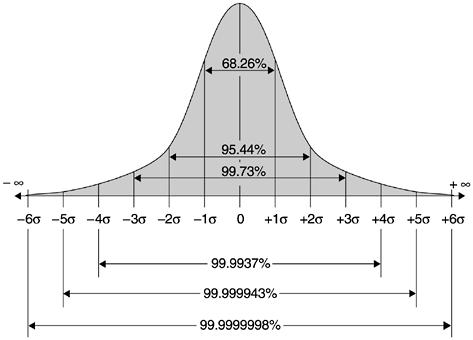
\includegraphics[width=\linewidth, height=1.5in, keepaspectratio]{../figure/sixsigma.jpg}
\caption{In the \emph{normal distribution} or the Bell curve, the
probability of deviating \(k\) standard deviations from the expectation
shrinks \emph{exponentially} in \(k^2\), and specifically with
probability at least \(1-2e^{-k^2/2}\), a random variable \(X\) of
expectation \(\mu\) and standard deviation \(\sigma\) satisfies
\(\mu -k\sigma \leq X \leq \mu+k\sigma\). This figure gives more precise
bounds for \(k=1,2,3,4,5,6\). (Image credit:Imran Baghirov)}
\label{empiricalbellfig}
\end{marginfigure}

The following extremely useful theorem shows that such exponential decay
occurs every time we have a sum of independent and bounded variables.
This theorem is known under many names in different communities, though
it is mostly called the
\href{https://en.wikipedia.org/wiki/Chernoff_bound}{Chernoff bound} in
the computer science literature:

\hypertarget{chernoffthm}{}
\begin{theorem}[Chernoff/Hoeffding bound] \label[theorem]{chernoffthm}

If \(X_1,\ldots,X_n\) are i.i.d random variables such that
\(X_i \in [0,1]\) and \(\E[X_i]=p\) for every \(i\), then for every
\(\epsilon >0\) \[
\Pr[ \left| \sum_{i=0}^{n-1} X_i - pn \right| > \epsilon n ] \leq 2\cdot e^{-2\epsilon^2 n} .
\]

\end{theorem}

We omit the proof, which appears in many texts, and uses Markov's
inequality on i.i.d random variables \(Y_0,\ldots,Y_n\) that are of the
form \(Y_i = e^{\lambda X_i}\) for some carefully chosen parameter
\(\lambda\). See \cref{chernoffstirlingex} for a proof of the simple
(but highly useful and representative) case where each \(X_i\) is
\(\{0,1\}\) valued and \(p=1/2\). (See also \cref{poorchernoff} for a
generalization.)

\section{Exercises}\label{Exercises}

\begin{exercise} \label[exercise]{Prove-that-for-every-finite-ST}

Prove that for every finite \(S,T\), there are \((|T|+1)^{|S|}\) partial
functions from \(S\) to \(T\).

\end{exercise}

\hypertarget{ohnotationex}{}
\begin{exercise}[$O$-notation] \label[exercise]{ohnotationex}

For every pair of functions \(F,G\) below, determine which of the
following relations holds: \(F=O(G)\), \(F=\Omega(G)\), \(F=o(G)\) or
\(F=\omega(G)\).

\begin{enumerate}
\def\labelenumi{\alph{enumi}.}
\item
  \(F(n)=n\), \(G(n)=100n\).
\item
  \(F(n)=n\), \(G(n)=\sqrt{n}\).
\item
  \(F(n)=n\log n\), \(G(n)=2^{(\log (n))^2}\).
\item
  \(F(n)=\sqrt{n}\), \(G(n)=2^{\sqrt{\log n}}\)
\item
  \(F(n) = \binom{n}{\ceil{0.2 n}}\) , \(G(n) = 2^{0.1 n}\) (where
  \(\binom{n}{k}\) is the number of \(k\)-sized subsets of a set of size
  \(n\)) and \(g(n) = 2^{0.1 n}\). See footnote for hint.\footnote{one
    way to do this is to use \href{https://goo.gl/cqEmS2}{Stirling's
    approximation for the factorial function.}.}
\end{enumerate}

\end{exercise}

\begin{exercise} \label[exercise]{Give-an-example-of-a-pair-of-f}

Give an example of a pair of functions \(F,G:\N \rightarrow \N\) such
that neither \(F=O(G)\) nor \(G=O(F)\) holds.

\end{exercise}

\hypertarget{propexpecvariance}{}
\begin{exercise}[Properties of expectation and variance] \label[exercise]{propexpecvariance}

In the following exercise \(X,Y\) denote random variables over some
sample space \(S\). You can assume that the probability on \(S\) is the
uniform distribution--- every point \(s\) is output with probability
\(1/|S|\). Thus \({\mathbb{E}}[X]= (1/|S|)\sum_{s\in S}X(s)\). We define
the variance and standard deviation of \(X\) and \(Y\) as above (e.g.,
\(Var[X] = {\mathbb{E}}[(X-{\mathbb{E}}[X])^2 ]\) and the standard
deviation is the square root of the variance). You can reuse your
answers to prior questions in the later ones.

\begin{enumerate}
\def\labelenumi{\arabic{enumi}.}
\item
  Prove that \(Var[X]\) is always non-negative.
\item
  Prove that \(Var[X] = {\mathbb{E}}[X^2] - {\mathbb{E}}[X]^2\).
\item
  Prove that always \({\mathbb{E}}[X^2] \geq {\mathbb{E}}[X]^2\).
\item
  Give an example for a random variable \(X\) such that
  \({\mathbb{E}}[X^2] > {\mathbb{E}}[X]^2\).
\item
  Give an example for a random variable \(X\) such that its standard
  deviation is \emph{not equal} to
  \({\mathbb{E}}[ | X - {\mathbb{E}}[X] | ]\).
\item
  Give an example for a random variable \(X\) such that its standard
  deviation is \emph{equal to} to
  \({\mathbb{E}}[ | X - {\mathbb{E}}[X] | ]\).
\item
  Give an example for two random variables \(X,Y\) such that
  \({\mathbb{E}}[\ensuremath{\mathit{XY}}] = {\mathbb{E}}[X]{\mathbb{E}}[Y]\).
\item
  Give an example for two random variables \(X,Y\) such that
  \({\mathbb{E}}[\ensuremath{\mathit{XY}}] \neq {\mathbb{E}}[X]{\mathbb{E}}[Y]\).
\item
  Prove that if \(X\) and \(Y\) are independent random variables (i.e.,
  for every \(x,y\), \(\Pr[X=x \wedge Y=y]=\Pr[X=x]\Pr[Y=y]\)) then
  \({\mathbb{E}}[\ensuremath{\mathit{XY}}]={\mathbb{E}}[X]{\mathbb{E}}[Y]\)
  and \(Var[X+Y]=Var[X]+Var[Y]\).
\end{enumerate}

\end{exercise}

\hypertarget{randomfunction}{}
\begin{exercise}[Random hash function] \label[exercise]{randomfunction}

Suppose that \(H\) is chosen to be a random function mapping the numbers
\(\{1,\ldots,n\}\) to the numbers \(\{1,..,m \}\). That is, for every
\(i\in \{1,\ldots,n\}\), \(H(i)\) is chosen to be a random number in
\(\{ 1,\ldots, m\}\) and that choice is done independently for every
\(i\). For every \(i<j \in \{1,\ldots,n\}\), define the random variable
\(X_{i,j}\) to equal \(1\) if there was a \emph{collision} between
\(H(i)\) and \(H(j)\) in the sense that \(H(i)=H(j)\) and to equal \(0\)
otherwise.

\begin{enumerate}
\def\labelenumi{\arabic{enumi}.}
\item
  For every \(i<j\), compute \({\mathbb{E}}[ X_{i,j} ]\).
\item
  Define \(Y = \sum_{i<j} X_{i,j}\) to be the total number of
  collisions. Compute \({\mathbb{E}}[ Y ]\) as a function of \(n\) and
  \(m\). In particular your answer should imply that if \(m < n^2/1000\)
  then \({\mathbb{E}}[Y]>1\) and hence in expectation there should be at
  least one collision and so the function \(H\) will not be one to one.
\item
  Prove that if \(m > 1000\cdot n^2\) then the probability that \(H\) is
  one to one is at least \(0.9\).
\item
  Give an example of a random variable \(Z\) (unrelated to the function
  \(H\)) that is always equal to a non-negative integer, and such that
  \({\mathbb{E}}[Z] \geq 1000\) but \(\Pr[ Z > 0] < 0.001\).
\item
  Prove that if \(m < n^2/1000\) then the probability that \(H\) is one
  to one is at most \(0.1\).
\end{enumerate}

\end{exercise}

\section{Exercises}\label{Exercises}

\begin{exercise} \label[exercise]{Suppose-that-we-toss-three-ind}

Suppose that we toss three independent fair coins \(a,b,c \in \{0,1\}\).
What is the probability that the XOR of \(a\),\(b\), and \(c\) is equal
to \(1\)? What is the probability that the AND of these three values is
equal to \(1\)? Are these two events independent?

\end{exercise}

\begin{exercise} \label[exercise]{Give-an-example-of-random-vari}

Give an example of random variables \(X,Y: \{0,1\}^3 \rightarrow \R\)
such that \(\E[\ensuremath{\mathit{XY}}] \neq \E[X]\E[Y]\).

\end{exercise}

\hypertarget{noindnocorex}{}
\begin{exercise} \label[exercise]{noindnocorex}

Give an example of random variables \(X,Y: \{0,1\}^3 \rightarrow \R\)
such that \(X\) and \(Y\) are \emph{not} independent but
\(\E[\ensuremath{\mathit{XY}}] =\E[X]\E[Y]\).

\end{exercise}

\hypertarget{expprodex}{}
\begin{exercise}[Product of expectations] \label[exercise]{expprodex}

Prove \cref{expprod}

\end{exercise}

\hypertarget{indeplemex}{}
\begin{exercise}[Transformations preserve independence] \label[exercise]{indeplemex}

Prove \cref{indeplem}

\end{exercise}

\hypertarget{varianceex}{}
\begin{exercise}[Variance of independent random variables] \label[exercise]{varianceex}

Prove that if \(X_0,\ldots,X_{n-1}\) are independent random variables
then
\(\mathrm{Var}[X_0+\cdots+X_{n-1}]=\sum_{i=0}^{n-1} \mathrm{Var}[X_i]\).

\end{exercise}

\hypertarget{entropyex}{}
\begin{exercise}[Entropy (challenge)] \label[exercise]{entropyex}

Recall the definition of a distribution \(\mu\) over some finite set
\(S\). Shannon defined the \emph{entropy} of a distribution \(\mu\),
denoted by \(H(\mu)\), to be \(\sum_{x\in S} \mu(x)\log(1/\mu(x))\). The
idea is that if \(\mu\) is a distribution of entropy \(k\), then
encoding members of \(\mu\) will require \(k\) bits, in an amortized
sense. In this exercise we justify this definition. Let \(\mu\) be such
that \(H(\mu)=k\).\\
1. Prove that for every one to one function
\(F:S \rightarrow \{0,1\}^*\), \(\E_{x \sim \mu} |F(x)| \geq k\).\\
2. Prove that for every \(\epsilon\), there is some \(n\) and a
one-to-one function \(F:S^n \rightarrow \{0,1\}^*\), such that
\(\E_{x\sim \mu^n} |F(x)| \leq n(k+\epsilon)\), where \(x \sim \mu\)
denotes the experiments of choosing \(x_0,\ldots,x_{n-1}\) each
independently from \(S\) using the distribution \(\mu\).

\end{exercise}

\hypertarget{entropybinomex}{}
\begin{exercise}[Entropy approximation to binomial] \label[exercise]{entropybinomex}

Let \(H(p) = p \log(1/p)+(1-p)\log(1/(1-p))\).\footnote{While you don't
  need this to solve this exercise, this is the function that maps \(p\)
  to the entropy (as defined in \cref{entropyex}) of the \(p\)-biased
  coin distribution over \(\{0,1\}\), which is the function
  \(\mu:\{0,1\}\rightarrow [0,1]\) s.y. \(\mu(0)=1-p\) and \(\mu(1)=p\).}

Prove that for every \(p \in (0,1)\) and \(\epsilon>0\), if \(n\) is
large enough then\footnote{\textbf{Hint:} Use Stirling's formula for
  approximating the factorial function.} \[
2^{(H(p)-\epsilon)n }\binom{n}{pn} \leq 2^{(H(p)+\epsilon)n}
\] where \(\binom{n}{k}\) is the binomial coefficient
\(\tfrac{n!}{k!(n-k)!}\) which is equal to the number of \(k\)-size
subsets of \(\{0,\ldots,n-1\}\).

\end{exercise}

\hypertarget{chernoffstirlingex}{}
\begin{exercise}[Chernoff using Stirling] \label[exercise]{chernoffstirlingex}

\begin{enumerate}
\def\labelenumi{\arabic{enumi}.}
\item
  Prove that
  \(\Pr_{x\sim \{0,1\}^n}[ \sum x_i = k ] = \binom{n}{k}2^{-n}\).\\
\item
  Use this and \cref{entropybinomex} to prove (an approximate version
  of) the Chernoff bound for the case that \(X_0,\ldots,X_{n-1}\) are
  i.i.d. random variables over \(\{0,1\}\) each equaling \(0\) and \(1\)
  with probability \(1/2\). That is, prove that for every
  \(\epsilon>0\), and \(X_0,\ldots,X_{n-1}\) as above,
  \(\Pr[ |\sum_{i=0}^{n-1} - \tfrac{n/2}| > \epsilon n] < 2^{0.1 \cdot \epsilon^2 n}\).
\end{enumerate}

\end{exercise}

\hypertarget{poorchernoff}{}
\begin{exercise}[Poor man's Chernoff] \label[exercise]{poorchernoff}

\cref{chernoffstirlingex} establishes the Chernoff bound for the case
that \(X_0,\ldots,X_{n-1}\) are i.i.d variables over \(\{0,1\}\) with
expectation \(1/2\). In this exercise we use a slightly different method
(bounding the \emph{moments} of the random variables) to establish a
version of Chernoff where the random variables range over \([0,1]\) and
their expectation is some number \(p \in [0,1]\) that may be different
than \(1/2\). Let \(X_0,\ldots,X_{n-1}\) be i.i.d random variables with
\(\E X_i = p\) and \(\Pr [ 0 \leq X_i \leq 1 ]=1\). Define
\(Y_i = X_i - p\).

\begin{enumerate}
\def\labelenumi{\arabic{enumi}.}
\item
  Prove that for every \(j_0,\ldots,j_{n-1} \in \N\), if there exists
  one \(i\) such that \(j_i\) is odd then
  \(\E [\prod_{i=0}^{n-1} Y_i^{j_i}] = 0\).\\
\item
  Prove that for every \(k\),
  \(\E[ (\sum_{i=0}^{n-1} Y_i)^k ] \leq (10kn)^{k/2}\).\footnote{\textbf{Hint:}
    Bound the number of tuples \(j_0,\ldots,j_{n-1}\) such that every
    \(j_i\) is even and \(\sum j_i = k\) using the Binomial coefficient
    and the fact that in any such tuple there are at most \(k/2\)
    distinct indices.}\\
\item
  Prove that for every \(\epsilon>0\),
  \(\Pr[ |\sum_i Y_i| \geq \epsilon n ] \geq 2^{-\epsilon^2 n / (10000\log 1/\epsilon)}\).\footnote{\textbf{Hint:}
    Set \(k=2\lceil \epsilon^2 n /1000 \rceil\) and then show that if
    the event \(|\sum Y_i | \geq \epsilon n\) happens then the random
    variable \((\sum Y_i)^k\) is a factor of \(\epsilon^{-k}\) larger
    than its expectation.}
\end{enumerate}

\end{exercise}

\hypertarget{lowerboundcoins}{}
\begin{exercise}[Lower bound for distinguishing coins] \label[exercise]{lowerboundcoins}

The Chernoff bound can be used to show that if you were given a coin of
bias at least \(\epsilon\), you should only need \(O(1/\epsilon^2)\)
samples to be able to reject the ``null hypothesis'' that the coin is
completely unbiased with extremely high confidence. In the following
somewhat more challenging question, we try to show a converse to this,
proving that distinguishing between a fair every coin and a coin that
outputs ``heads'' with probability \(1/2 + \epsilon\) requires at least
\(\Omega(1/\epsilon^2)\) samples.

Let \(P\) be the uniform distribution over \({\{0,1\}}^n\) and \(Q\) be
the \(1/2+\epsilon\)-biased distribution corresponding to tossing \(n\)
coins in which each one has a probability of \(1/2+\epsilon\) of
equalling \(1\) and probability \(1/2-\epsilon\) of equalling \(0\).
Namely the probability of \(x\in{\{0,1\}}^n\) according to \(Q\) is
equal to \(\prod_{i=1}^n (1/2 - \epsilon + 2\epsilon x_i)\).

\begin{enumerate}
\def\labelenumi{\arabic{enumi}.}
\item
  Prove that for every threshold \(\theta\) between \(0\) and \(n\), if
  \(n < 1/(100\epsilon)^2\) then the probabilities that
  \(\sum x_i \leq \theta\) under \(P\) and \(Q\) respectively differ by
  at most \(0.1\). Therefore, one cannot use the test whether the number
  of heads is above or below some threshold to reliably distinguish
  between these two possibilities unless the number of samples \(n\) of
  the coins is at least some constant times \(1/\epsilon^2\).
\item
  Prove that for \emph{every} function \(F\) mapping \({\{0,1\}}^n\) to
  \({\{0,1\}}\), if \(n < 1/(100\epsilon)^2\) then the probabilities
  that \(F(x)=1\) under \(P\) and \(Q\) respectively differ by at most
  \(0.1\). Therefore, if the number of samples is smaller than a
  constant times \(1/\epsilon^2\) then there is simply \emph{no test}
  that can reliably distinguish between these two possiblities.
\end{enumerate}

\end{exercise}

\hypertarget{coindistex}{}
\begin{exercise}[Simulating distributions using coins] \label[exercise]{coindistex}

Our model for probability involves tossing \(n\) coins, but sometimes
algorithms require sampling from other distributions, such as selecting
a uniform number in \(\{0,\ldots,M-1\}\) for some \(M\). Fortunately, we
can simulate this with an exponentially small probability of error:
prove that for every \(M\), if \(n>k\lceil \log M \rceil\), then there
is a function
\(F:\{0,1\}^n \rightarrow \{0,\ldots,M-1\} \cup \{ \bot \}\) such that
\textbf{(1)} The probability that \(F(x)=\bot\) is at most \(2^{-k}\)
and \textbf{(2)} the distribution of \(F(x)\) conditioned on
\(F(x) \neq \bot\) is equal to the uniform distribution over
\(\{0,\ldots,M-1\}\).\footnote{\textbf{Hint:} Think of
  \(x\in \{0,1\}^n\) as choosing \(k\) numbers
  \(y_1,\ldots,y_k \in \{0,\ldots, 2^{\lceil \log M \rceil}-1 \}\).
  Output the first such number that is in \(\{0,\ldots,M-1\}\).}

\end{exercise}

\hypertarget{samplingex}{}
\begin{exercise}[Sampling] \label[exercise]{samplingex}

Suppose that a country has 300,000,000 citizens, 52 percent of which
prefer the color ``green'' and 48 percent of which prefer the color
``orange''. Suppose we sample \(n\) random citizens and ask them their
favorite color (assume they will answer truthfully). What is the
smallest value \(n\) among the following choices so that the probability
that the majority of the sample answers ``green'' is at most \(0.05\)?

\begin{enumerate}
\def\labelenumi{\alph{enumi}.}
\item
  1,000
\item
  10,000
\item
  100,000
\item
  1,000,000
\end{enumerate}

\end{exercise}

\hypertarget{exid}{}
\begin{exercise} \label[exercise]{exid}

Would the answer to \cref{samplingex} change if the country had
300,000,000,000 citizens?

\end{exercise}

\hypertarget{exidtwo}{}
\begin{exercise}[Sampling (2)] \label[exercise]{exidtwo}

Under the same assumptions as \cref{samplingex}, what is the smallest
value \(n\) among the following choices so that the probability that the
majority of the sample answers ``green'' is at most \(2^{-100}\)?

\begin{enumerate}
\def\labelenumi{\alph{enumi}.}
\item
  1,000
\item
  10,000
\item
  100,000
\item
  1,000,000
\item
  It is impossible to get such low probability since there are fewer
  than \(2^{100}\) citizens.
\end{enumerate}

\end{exercise}


\part{Private key cryptography}

\chapter{Computational Security}\label{2-Computational-Security}

\paragraph{Additional reading:} Sections 2.2 and 2.3 in Boneh-Shoup
book. Chapter 3 up to and including Section 3.3 in Katz-Lindell book.

Recall our cast of characters- Alice and Bob want to communicate
securely over a channel that is monitored by the nosy Eve. In the last
lecture, we have seen the definition of \emph{perfect secrecy} that
guarantees that Eve cannot learn \emph{anything} about their
communication beyond what she already knew. However, this security came
at a price. For every bit of communication, Alice and Bob have to
exchange in advance a bit of a secret key. In fact, the proof of this
result gives rise to the following simple Python program that can break
every encryption scheme that uses, say, a \(128\) bit key, with a
\(129\) bit message:

\begin{code}
from itertools import product # Import an iterator for cartesian products
from random import choice # choose random element of list

# Gets ciphertext as input and two potential plaintexts
# Returns most likely plaintext 
# We assume we have access to the function Encrypt(key,ciphertext)
def Distinguish(ciphertext,plaintext1,plaintext2):
    for key in product([0,1], repeat = 128): # Iterate over all possible keys of length 128
        if Encrypt(key, plaintext1)==ciphertext:
            return plaintext1
        if Encrypt(key, plaintext2)==ciphertext:
            return plaintext2
    return choice([plaintext1,plaintext2])
\end{code}

The program \texttt{Distinguish} will break any \(128\)-bit key and
\(129\)-bit message encryption
\texttt{Encrypt', in the sense that there exist  a pair of messages \$m\_0,m\_1\$ such that}Distinguish'\((E_k(m_b),m_0,m_1)=m_b\)
with probability at least \(0.75\) over \(k \leftarrow_R \{0,1\}^n\) and
\(b \leftarrow_R \{0,1\}\).

Now, generating, distributing, and protecting huge keys causes immense
logistical problems, which is why almost all encryption schemes used in
practice do in fact utilize short keys (e.g., \(128\) bits long) with
messages that can be much longer (sometimes even terabytes or more of
data).

So, why can't we use the above Python program to break all encryptions
in the Internet and win infamy and fortune? We can in fact, but we'll
have to wait a \emph{really} long time, since the loop in
\texttt{Distinguish} will run \(2^{128}\) times, which will take much
more than the lifetime of the universe to complete, even if we used all
the computers on the planet.

However, the fact that \emph{this} particular program is not a feasible
attack, does not mean there does not exist a different attack. But this
still suggests a tantalizing possibility: if we consider a relaxed
version of perfect secrecy that restricts Eve to performing computations
that can be done in this universe (e.g., less than \(2^{256}\) steps
should be safe not just for human but for all potential alien
civilizations) then can we bypass the impossibility result and allow the
key to be much shorter than the message?

This in fact does seem to be the case, but as we've seen, defining
security is a subtle task, and will take some care. As before, the way
we avoid (at least some of) the pitfalls of so many cryptosystems in
history is that we insist on very precisely \emph{defining} what it
means for a scheme to be secure.

Let us defer the discussion how one defines a function being computable
in ``less than \(T\) operations'' and just say that there is a way to
formally do so. We will want to say that a scheme has ``\(256\) bits of
security'' if it is not possible to break it using less than \(2^{256}\)
operations, and more generally that it has \(t\) bits of security if it
can't be broken using less than \(2^t\) operations. Given the perfect
secrecy definition we saw last time, a natural attempt for defining
Computational secrecy would be the following:

\hypertarget{firstcompdef}{}
\begin{definition}[Computational secrecy (first attempt)] \label[definition]{firstcompdef}

An encryption scheme \((E,D)\) has \emph{\(t\) bits of computational
secrecy} if for every two distinct plaintexts
\(\{m_0,m_1\} \subseteq {\{0,1\}}^\ell\) and every strategy of Eve using
at most \(2^t\) computational steps, if we choose at random
\(b\in{\{0,1\}}\) and a random key \(k\in{\{0,1\}}^n\), then the
probability that Eve guesses \(m_b\) after seeing \(E_k(m_b)\) is at
most \(1/2\).

\end{definition}

\paragraph{Note:} It is important to keep track of what is known and
unknown to the adversary Eve. The adversary knows the set
\(\{ m_0,m_1 \}\) of potential messages, and the ciphertext
\(y=E_k(m_b)\). The only things she doesn't know are whether \(b=0\) or
\(b=1\), and the value of the secret key \(k\). In particular, because
\(m_0\) and \(m_1\) are known to Eve, it does not matter whether we
define Eve's goal in this ``security game'' as outputting \(m_b\) or as
outputting \(b\).

\cref{firstcompdef} seems very natural, but is in fact \emph{impossible}
to achieve if the key is shorter than the message.

\begin{pause} \label[pause]{2-Before-reading-further}

Before reading further, you might want to stop and think if you can
\emph{prove} that there is no, say, encryption scheme with \(\sqrt{n}\)
bits of computational security satisfying \cref{firstcompdef} with
\(\ell = n+1\) and where the time to compute the encryption is
polynomial.

\end{pause}

The reason \cref{firstcompdef} can't be achieved that if the message is
even one bit longer than the key, we can always have a very efficient
procedure that achieves success probability of about \(1/2 + 2^{-n-1}\)
by guessing the key. This is because we can replace the loop in the
Python program \texttt{Distinguish} by choosing the key at random. Since
we have some small chance of guessing correctly, we will get a small
advantage over half.

Of course an advantage of \(2^{-256}\) in guessing the message is not
really something we would worry about. For example, since the earth is
about 5 billion years old, we can estimate the chance that an asteroid
of the magnitude that caused the dinosaurs' extinction will hit us this
very second to be about \(2^{-60}\). Hence we want to relax the notion
of computational security so it would not consider guessing with such a
tiny advantage as a ``true break'' of the scheme. The resulting
definition is the following:

\hypertarget{compsecconcdef}{}
\begin{definition}[Computational secrecy (concrete)] \label[definition]{compsecconcdef}

An encryption scheme \((E,D)\) has \emph{\(t\) bits of computational
secrecy\footnote{Another version of ``\(t\) bits of security'' is that a
  scheme has \(t\) bits of security if for every \(t_1+t_2 \leq t\), an
  attacker running in \(2^{t_1}\) time can't get success probability
  advantage more than \(2^{-t_2}\). However these two definitions only
  differ from one another by at most a factor of two. This may be
  important for practical applications (where the difference between
  \(64\) and \(32\) bits of security could be crucial) but won't matter
  for our concerns.}} if for every two distinct plaintexts
\(\{m_0,m_1\} \subseteq {\{0,1\}}^\ell\) and every strategy of Eve using
at most \(2^t\) computational steps, if we choose at random
\(b\in{\{0,1\}}\) and a random key \(k\in{\{0,1\}}^n\), then the
probability that Eve guesses \(m_b\) after seeing \(E_k(m_b)\) is at
most \(1/2+2^{-t}\).

\end{definition}

Having learned our lesson, let's try to see that this strategy does give
us the kind of conditions we desired. In particular, let's verify that
this definition implies the analogous condition to perfect secrecy.

\hypertarget{twotomanycomp}{}
\begin{theorem}[Guessing game for computational secrecy] \label[theorem]{twotomanycomp}

If \((E,D)\) has \(t\) bits of Computational secrecy as per
\cref{compsecconcdef} then for every subset
\(M \subseteq {\{0,1\}}^\ell\) and every strategy of Eve using at most
\(2^t-(100\ell+100)\) computational steps, if we choose at random
\(m\in M\) and a random key \(k\in{\{0,1\}}^n\), then the probability
that Eve guesses \(m\) after seeing \(E_k(m)\) is at most
\(1/|M|+2^{-t+1}\).

\end{theorem}

Before proving this theorem note that it gives us a pretty strong
guarantee. In the exercises we will strengthen it even further showing
that no matter what prior information Eve had on the message before, she
will never get any non-negligible new information on it.\footnote{The
  latter property is known as ``semantic security'', see also section
  3.2.2 of Katz Lindell on ``semantic security'' and Section 2 of
  Boneh-Shoup ``computational ciphers and semantic security''.} One way
to phrase it is that if the sender used a \(256\)-bit secure encryption
to encrypt a message, then your chances of getting to learn any
additional information about it before the universe collapses are more
or less the same as the chances that a fairy will materialize and
whisper it in your ear.

\begin{pause} \label[pause]{2-Before-reading-the-pro}

Before reading the proof, try to again review the proof of
\cref{twotomanythm}, and see if you can generalize it yourself to the
computational setting.

\end{pause}

\begin{proof}[Proof of \cref{twotomanycomp}] \label[proof]{2-The-proof-is-rather-si}

The proof is rather similar to the equivalence of guessing one of two
messages vs.~one of many messages for perfect secrecy (i.e.,
\cref{twotomanythm}). However, in the computational context we need to
be careful in keeping track of Eve's running time. In the proof of
\cref{twotomanythm} we showed that if there exists:

\begin{itemize}
\tightlist
\item
  A subset \(M\subseteq {\{0,1\}}^\ell\) of messages
\end{itemize}

and

\begin{itemize}
\item
  An adversary \(Eve:{\{0,1\}}^o\rightarrow{\{0,1\}}^\ell\) such that

  \begin{equation*}
  \Pr_{m{\leftarrow_{\tiny R}}M, k{\leftarrow_{\tiny R}}{\{0,1\}}^n}[ Eve(E_k(m))=m ] > 1/|M|
  \end{equation*}
\end{itemize}

Then there exist two messages \(m_0,m_1\) and an adversary
\(Eve':{\{0,1\}}^o\rightarrow{\{0,1\}}^\ell\) such that
\(\Pr_{b{\leftarrow_{\tiny R}}{\{0,1\}},k{\leftarrow_{\tiny R}}{\{0,1\}}^n}[Eve'(E_k(m_b))=m_b ] > 1/2\).

To adapt this proof to the computational setting and complete the proof
of the current theorem it suffices to show that:

\begin{itemize}
\item
  If the probability of \(Eve\) succeeding was
  \(\tfrac{1}{|M|} + \epsilon\) then the probability of \(Eve'\)
  succeeding is at least \(\tfrac{1}{2} + \epsilon/2\).
\item
  If \(Eve\) can be computed in \(T\) operations, then \(Eve'\) can be
  computed in \(T + 100\ell + 100\) operations.
\end{itemize}

This will imply that if \(Eve\) ran in polynomial time and had
polynomial advantage over \(1/|M|\) in guessing a plaintext chosen from
\(M\), then \(Eve'\) would run in polynomial time and have polynomial
advantage over \(1/2\) in guessing a plaintext chosen from
\(\{ m_0,m_1\}\).

The first item can be shown by simply doing the same proof more
carefully, keeping track how the advantage over \(\tfrac{1}{|M|}\) for
\(Eve\) translates into an advantage over \(\tfrac{1}{2}\) for \(Eve'\).
As the world's most annoying saying goes, doing this is an excellent
exercise for the reader.

The second item is obtained by looking at the definition of \(Eve'\)
from that proof. On input \(c\), \(Eve'\) computed \(m=Eve(c)\) (which
costs \(T\) operations), checked if \(m=m_0\) (which costs, say, at most
\(5\ell\) operations), and then outputted either \(1\) or a random bit
(which is a constant, say at most \(100\) operations).

\end{proof}

\subsection{Proof by reduction}\label{2-Proof-by-reduction}

The proof of \cref{twotomanycomp} is a model to how a great many of the
results in this course will look like. Generally we will have many
theorems of the form:

\begin{quote}
``If there is a scheme \(S'\) satisfying security definition \(X'\) then
there is a scheme \(S\) satisfying security definition \(X\)''
\end{quote}

In the context of \cref{twotomanycomp}, \(X'\) was ``having \(t\) bits
of security'' (in the context distinguishing between encryptions of two
ciphertexts) and \(X\) was the more general notion of hardness of
getting a non-trivial advantage over guessing for an encryption of a
random \(m\in M\). While in \cref{twotomanycomp} the encryption scheme
\(S\) was the same as \(S'\), this need not always be the case. However,
all of the proofs of such statements will have the same global
structure--- we will assume towards a contradiction, that there is an
efficient adversary strategy \(Eve\) demonstrating that the scheme \(S\)
violates the security notion \(X\), and build from \(Eve\) a strategy
\(Eve'\) demonstrating that \(S'\) violates \(X'\). This is such an
important point that it deserves repeating:

\begin{quote}
\emph{The way you show that if \(S'\) is secure then \(S\) is secure is
by giving a transformation from an adversary that breaks \(S\) into an
adversary that breaks \(S'\)}
\end{quote}

For computational secrecy, we will always want that \(Eve'\) will be
efficient if \(Eve\) is, and that will usually be the case because
\(Eve'\) will simply use \(Eve\) as a black box, which it will not
invoke too many times, and addition will use some polynomial time
preprocessing and postprocessing. The more challenging parts of such
proofs are typically:

\begin{itemize}
\item
  Coming up with the strategy \(Eve'\).
\item
  Analyzing the probability of success and in particular showing that if
  \(Eve\) had non-negligible advantage then so will \(Eve'\).
\end{itemize}

\begin{marginfigure}
\centering
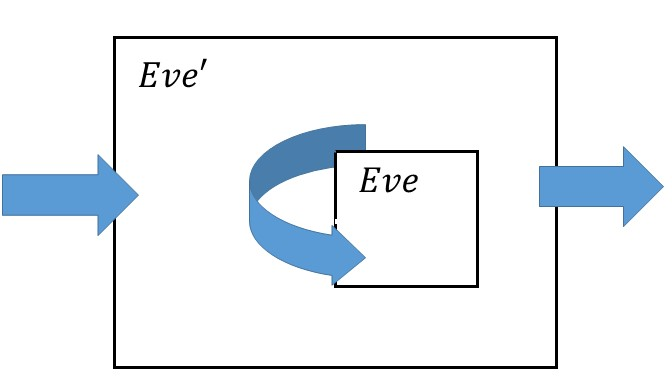
\includegraphics[width=\linewidth, height=1.5in, keepaspectratio]{../figure/reduction.jpg}
\caption{We show that the security of \(S'\) implies the security of
\(S\) by transforming an adversary \(Eve\) breaking \(S\) into an
adversary \(Eve'\) breaking \(S'\).}
\label{reductiongenfig}
\end{marginfigure}

Note that, just like in the context of NP completeness or
uncomputability reductions, security reductions work \emph{backwards}.
That is, we construct the scheme \(S\) based on the scheme \(S'\), but
then prove that we can transform an algorithm breaking \(S\) into an
algorithm breaking \(S'\). Just like in computational complexity, it can
sometimes be hard to keep track of the direction of the reduction. In
fact, cryptographic reductions can be even subtler, since they involve
an interplay of several entities (for example, sender, receiver, and
adversary) and probabilistic choices (e.g., over the message to be sent
and the key).

\section{The asymptotic approach}\label{2-The-asymptotic-approac}

For practical security, often every bit of security matters. We want our
keys to be as short as possible and our schemes to be as fast as
possible while satisfying a particular level of security. In practice we
would usually like to ensure that when we use a smallish security
parameter such as \(n\) in the few hundreds or thousands then:

\begin{itemize}
\item
  The \emph{honest parties} (the parties running the encryption and
  decryption algorithms) are extremely efficient, something like
  100-1000 cycles per byte of data processed. In theory terms we would
  want them be using an \(O(n)\) or at worst \(O(n^2)\) time algorithms
  with not-too-big hidden constants.
\item
  We want to protect against \emph{adversaries} (the parties trying to
  break the encryption) that have much vaster computational
  capabilities. A typical modern encryption is built so that using
  standard key sizes it can withstand the combined computational powers
  of all computers on earth for several decades. In theory terms we
  would want the time to break the scheme to be \(2^{\Omega(n)}\) (or if
  not, at least \(2^{\Omega(\sqrt{n})}\) or \(2^{\Omega(n^{1/3})}\))
  with not too small hidden constants.
\end{itemize}

For implementing cryptography in practice, the tradeoff between security
and efficiency can be crucial. However, for understanding the
\emph{principles} behind cryptography, keeping track of concrete
security can be a distraction, and so just like we do in algorithms
courses, we will use \emph{asymptotic analysis} (also known as \emph{big
Oh notation}) to sweep many of those details under the carpet.

To a first approximation, there will be only two types of running times
we will encounter in this course:

\begin{itemize}
\item
  \emph{Polynomial} running time of the form \(d\cdot n^c\) for some
  constants \(d,c>0\) (or \(poly(n)=n^{O(1)}\) for short), which we will
  consider as \emph{efficient}.
\item
  \emph{Exponential} running time of the form
  \(2^{d\cdot n^{\epsilon}}\) for some constants \(d,\epsilon >0\) (or
  \(2^{n^{\Omega(1)}}\) for short) which we will consider as
  \emph{infeasible}.\footnote{Some texts reserve the term
    \emph{exponential} to functions of the form \(2^{\epsilon n}\) for
    some \(\epsilon > 0\) and call a function such as, say,
    \(2^{\sqrt{n}}\) \emph{subexponential} . However, we will generally
    not make this distinction in this course.}
\end{itemize}

Another way to say it is that in this course, if a scheme has any
security at all, it will have at least \(n^{\epsilon}\) bits of security
where \(n\) is the length of the key and \(\epsilon>0\) is some absolute
constant such as \(\epsilon=1/3\). Hence in this course, whenever you
hear the term ``super polynomial'', you can equate it in your mind with
``exponential'' and you won't be far off the truth.

These are not all the theoretically possible running times. One can have
intermediate functions such as \(n^{\log n}\) though we will generally
not encounter those. To make things clean (and to correspond to standard
terminology), we will generally associate ``efficient computation'' with
\emph{polynomial time} in \(n\) where \(n\) is either its input length
or the key size (the key size and input length will always be
polynomially related, and so this choice won't matter). We want our
algorithms (encryption, decryption, etc.) to be computable in polynomial
time, but to require \emph{super polynomial time} to break.

\paragraph{Negligible probabilities.} In cryptography, we care not just
about the running time of the adversary but also about their probability
of success (which should be as small as possible). If
\(\mu:\N \rightarrow [0,\infty)\) is a function (which we'll often think
of as corresponding to the adversary's probability of success or
advantage over the trivial probability, as a function of the key size
\(n\)) then we say that \(\mu(n)\) is \emph{negligible} if it's smaller
than the inverse of every (positive) polynomial. Our security
definitions will have the following form:

\begin{quote}
\emph{"Scheme \(S\) is secure if for every polynomial \(p(\cdot)\) and
\(p(n)\) time adversary \(Eve\), there is some negligible function
\(\mu\) such that the probability that \(Eve\) succeeds in the security
game for \(S\) is at most \(trivial + \mu(n)\)}"
\end{quote}

We now make these notions more formal.

\hypertarget{negligibledef}{}
\begin{definition}[Negligible function] \label[definition]{negligibledef}

A function \(\mu:\mathbb{N} \rightarrow [0,\infty)\) is
\emph{negligible} if for every polynomial \(p:\N \rightarrow \N\) there
exists \(N \in \N\) such that \(\mu(n) < \tfrac{1}{p(n)}\) for every
\(n>N\).\footnote{Negligible functions are sometimes defined with image
  equalling \([0,1]\) as opposed to the set \([0,\infty)\) of
  non-negative real numbers, since they are typically used to bound
  probabilities. However, this does not make much difference since if
  \(\mu\) is negligible then for large enough \(n\), \(\mu(n)\) will be
  smaller than one.}

\end{definition}

The following exercise provides a good way to get some comfort with this
definition:

\hypertarget{negligible}{}
\begin{exercise}[Negligible functions properties] \label[exercise]{negligible}

\begin{enumerate}
\def\labelenumi{\arabic{enumi}.}
\item
  Let \(\mu:\N \rightarrow [0,\infty)\) be a negligible function. Prove
  that for every polynomials \(p,q:\R \rightarrow \R\) with non-negative
  coefficients such that \(p(0) = 0\), the function
  \(\mu':\N \rightarrow [0,\infty)\) defined as
  \(\mu'(n) = p(\mu(q(n)))\) is negligible.
\item
  Let \(\mu:\N \rightarrow [0,\infty)\). Prove that \(\mu\) is
  negligible if and only if for every constant \(c\),
  \(\lim_{n \rightarrow \infty} n^c \mu(n) = 0\).
\end{enumerate}

\end{exercise}

\hypertarget{asymptotic}{}
\begin{remark}[Asymptotic analysis] \label[remark]{asymptotic}

The above definitions could be confusing if you haven't encountered
asymptotic analysis before. Reading the beginning of Chapter 3 (pages
43-51) in the KL book, as well as the mathematical background lecture in
my \href{http://www.introtcs.org/public/index.html}{intro to TCS notes}
can be extremely useful. As a rule of thumb, if every time you see the
word ``polynomial'' you imagine the function \(n^{10}\) and every time
you see the word ``negligible'' you imagine the function
\(2^{-\sqrt{n}}\) then you will get the right intuition.

What you need to remember is that negligible is much smaller than any
inverse polynomial, while polynomials are closed under multiplication,
and so we have the ``equations''

\begin{equation*}
negligible\times polynomial = negligible
\end{equation*}

and

\begin{equation*}
polynomial \times polynomial = polynomial
\end{equation*}

As mentioned, in practice people really want to get as close as possible
to \(n\) bits of security with an \(n\) bit key, but we would be happy
as long as the security grows with the key, so when we say a scheme is
``secure'' you can think of it having \(\sqrt{n}\) bits of security
(though any function growing faster than \(\log n\) would be fine as
well).

\end{remark}

From now on, we will require all of our encryption schemes to be
\emph{efficient} which means that the encryption and decryption
algorithms should run in polynomial time. Security will mean that any
efficient adversary can make at most a negligible gain in the
probability of guessing the message over its a priori
probability.\footnote{Note that there is a subtle issue here with the
  order of quantifiers. For a scheme to be efficient, the algorithms
  such as encryption and decryption need to run in some \emph{fixed}
  polynomial time such as \(n^2\) or \(n^3\). In contrast we allow the
  adversary to run in \emph{any} polynomial time. That is, for every
  \(c\), if \(n\) is large enough, then the scheme should be secure
  against an adversary that runs in time \(n^c\). This is in line with
  the general principle in cryptography that we always allow the
  adversary potentially much more resources than those used by the
  honest users. In practical security we often assume that the gap
  between the honest use and the adversary resources can be
  \emph{exponential}. For example, a low power embedded device can
  encrypt messages that, as far as we know, are undecipherable even by a
  nation-state using super-computers and massive data centers.}

We can now formally define computational secrecy in asymptotic terms:

\hypertarget{compsecdef}{}
\begin{definition}[Computational secrecy (asymptotic)] \label[definition]{compsecdef}

An encryption scheme \((E,D)\) is \emph{computationally secret} if for
every two distinct plaintexts \(\{m_0,m_1\} \subseteq {\{0,1\}}^\ell\)
and every efficient (i.e., polynomial time) strategy of Eve, if we
choose at random \(b\in{\{0,1\}}\) and a random key \(k\in{\{0,1\}}^n\),
then the probability that Eve guesses \(m_b\) after seeing \(E_k(m_b)\)
is at most \(1/2+\mu(n)\) for some negligible function \(\mu(\cdot)\).

\end{definition}

\subsection{Counting number of operations.}\label{countoperation}

One more detail that we've so far ignored is what does it mean exactly
for a function to be computable using at most \(T\) operations.
Fortunately, when we don't really care about the difference between
\(T\) and, say, \(T^2\), then essentially every reasonable definition
gives the same answer.\footnote{With some caveats that need to be added
  due to \emph{quantum computers}: we'll get to those later in the
  course, though they won't change most of our theory. See also
  \href{https://introtcs.org/public/lec_04_code_and_data.html\#PECTTsec}{this
  discussion in my intro TCS textbook} and
  \href{https://www.scottaaronson.com/talks/bernays2.ppt}{this
  presentation of Aaronson} on the ``extended Church Turing thesis''.}
Formally, we can use the notions of Turing machines, Boolean circuits,
or straightline programs to define complexity. For concreteness, let's
define that a function \(F:{\{0,1\}}^n\rightarrow{\{0,1\}}^m\) has
complexity at most \(T\) if there is a Boolean circuit that computes
\(F\) using at most \(T\) Boolean gates (say AND/OR/NOT or NAND;
alternatively you can choose your favorite universal gate sets.) We will
often also consider \emph{probabilistic} functions in which case we
allow the circuit a RAND gate that outputs a single random bit (though
this in general does not give extra power). The fact that we only care
about asymptotics means you don't really need to think of gates when
arguing in cryptography. However, it is comforting to know that this
notion has a precise mathematical formulation.

\paragraph{Uniform vs non-uniform models.} While many computational
texts focus on models such as Turing machines, in cryptography it is
more convenient to use Boolean circuits which are a
\href{https://introtcs.org/public/lec_11_running_time.html\#nonuniformcompsec}{non
uniform model} of computation in the sense that we allow a different
circuit for every given input length. The reasons are the following:

\begin{enumerate}
\def\labelenumi{\arabic{enumi}.}
\item
  Circuits can express \emph{finite} computation, while Turing machines
  only make sense for computing on arbitrarily large input lengths, and
  so we can make sense of notions such as ``\(t\) bits of computational
  security''.
\item
  Circuits allow the notion of ``hardwiring'' whereby if we can compute
  a certain function \(F:\{0,1\}^{n+s} \rightarrow \{0,1\}^m\) using a
  circuit of \(T\) gates and have a string \(w \in \{0,1\}^s\) then we
  can compute the function \(x \mapsto F(xw)\) using \(T\) gates as
  well. This is useful in many cryptograhic proofs.
\end{enumerate}

One can build the theory of cryptography using Turing machines as well,
but it is more cumbersome.

\hypertarget{computebeyondfunctions}{}
\begin{remark}[Computing beyond functions] \label[remark]{computebeyondfunctions}

Later on in the course, both our cryptographic schemes and the
adversaries will extend beyond simple functions that map an input to an
output, and we will consider \emph{interactive algorithms} that exchange
messages with one another. Such an algorithm can be implemented using
circuits or Turing machines that take as input the prior state and the
history of messages up to a certain point in the interaction, and output
the next message in the interaction. The number of operations used in
such a strategy is the total number of gates used in computing all the
messages.

\end{remark}

\section{Our first conjecture}\label{2-Our-first-conjecture}

We are now ready to make our first conjecture:

\begin{quote}
\textbf{The Cipher Conjecture:}\footnote{As will be the case for other
  conjectures we talk about, the name ``The Cipher Conjecture'' is not a
  standard name, but rather one we'll use in this course. In the
  literature this conjecture is mostly referred to as the conjecture of
  existence of \emph{one way functions}, a notion we will learn about
  later. These two conjectures a priori seem quite different but have
  been shown to be equivalent.} There exists a computationally secret
encryption scheme \((E,D)\) (where \(E,D\) are efficient) with length
function \(\ell(n)=n+1\).
\end{quote}

A \emph{conjecture} is a well defined mathematical statement which (1)
we believe is true but (2) don't know yet how to prove. Proving the
cipher conjecture will be a great achievement and would in particular
settle the P vs NP question, which is arguably \emph{the} fundamental
question of computer science. That is, the following theorem is known:

\hypertarget{PNPcipherthm}{}
\begin{theorem}[Breaking crypto if P=NP] \label[theorem]{PNPcipherthm}

If \(P=\ensuremath{\mathit{NP}}\) then there does not exist a
computationally secret encryption with efficient \(E\) and \(D\) and
where the message is longer than the key.

\end{theorem}

\begin{proof} \label[proof]{2-We-just-sketch-the-pro}

We just sketch the proof, as this is not the focus of this course. If
\(P=\ensuremath{\mathit{NP}}\) then whenever we have a loop that
searches through some domain to find some string that satisfies a
particular property (like the loop in the \texttt{Distinguish}
subroutine above that searches over all keys) then this loop can be sped
up \emph{exponentially} .

\end{proof}

While it is very widely believed that
\(P\neq \ensuremath{\mathit{NP}}\), at the moment we do not know how to
\emph{prove} this, and so have to settle for accepting the cipher
conjecture as essentially an axiom, though we will see later in this
course that we can show it follows from some seemingly weaker
conjectures.

There are several reasons to believe the cipher conjecture. We now
briefly mention some of them:

\begin{itemize}
\item
  \emph{Intuition:} If the cipher conjecture is false then it means that
  for \emph{every} possible cipher we can make the exponential time
  attack described above become efficient. It seems ``too good to be
  true'' in a similar way that the assumption that P=NP seems too good
  to be true.
\item
  \emph{Concrete candidates:} As we will see in the next lecture, there
  are several concrete candidate ciphers using keys shorter than
  messages for which despite \emph{tons} of effort, no one knows how to
  break them. Some of them are widely used and hence governments and
  other benign or not so benign organizations have every reason to
  invest huge resources in trying to break them. Despite that as far as
  we know (and we know a little more after Edward Snowden's revelations)
  there is no significant break known for the most popular ciphers.
  Moreover, there are other ciphers that can be based on canonical
  mathematical problems such as factoring large integers or decoding
  random linear codes that are immensely interesting in their own right,
  independently of their cryptographic applications.
\item
  \emph{Minimalism:} Clearly if the cipher conjecture is false then we
  also don't have a secure encryption with a message, say, twice as long
  as the key. But it turns out the cipher conjecture is in fact
  \emph{necessary} for essentially every cryptographic primitive,
  including not just private key and public key encryptions but also
  digital signatures, hash functions, pseudorandom generators, and more.
  That is, if the cipher conjecture is false then to a large extent
  cryptography does not exist, and so we essentially have to assume this
  conjecture if we want to do any kind of cryptography.
\end{itemize}

\section{Why care about the cipher
conjecture?}\label{2-Why-care-about-the-cip}

\begin{quote}
\emph{``Give me a place to stand, and I shall move the world''}
Archimedes, circa 250 BC
\end{quote}

Every perfectly secure encryption scheme is clearly also computationally
secret, and so if we required a message of size \(n\) instead \(n+1\),
then the conjecture would have been trivially satisfied by the one-time
pad. However, having a message longer than the key by just a single bit
does not seem that impressive. Sure, if we used such a scheme with
\(128\)-bit long keys, our communication will be smaller by a factor of
\(128/129\) (or a saving of about \(0.8\%\)) over the one-time pad, but
this doesn't seem worth the risk of using an unproven conjecture.
However, it turns out that if we assume this rather weak condition, we
can actually get a computationally secret encryption scheme with a
message of size \(p(n)\) for \emph{every} polynomial \(p(\cdot)\). In
essence, we can fix a single \(n\)-bit long key and communicate securely
as many bits as we want!

Moreover, this is just the beginning. There is a huge range of other
useful cryptographic tools that we can obtain from this seemingly
innocent conjecture: (We will see what all these names and some of these
reductions mean later in the course.)

\begin{figure}
\centering
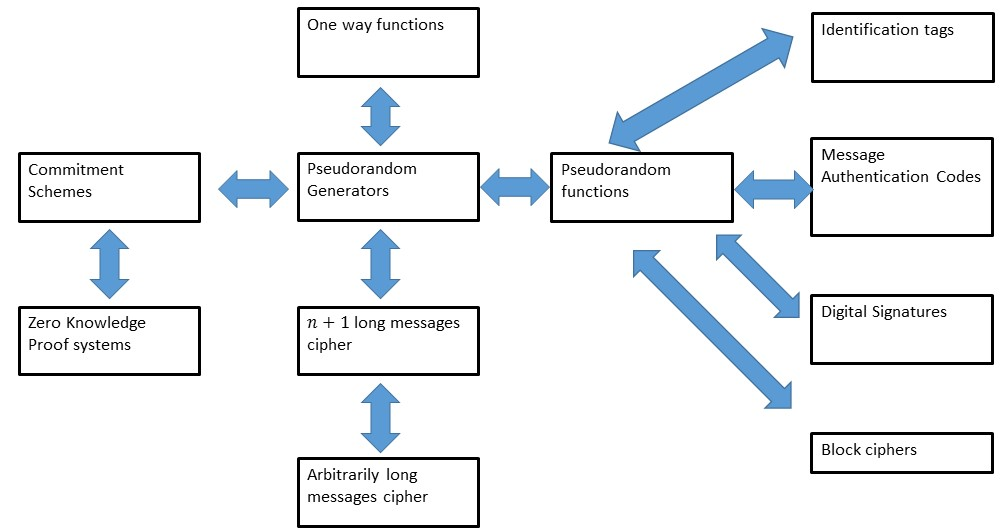
\includegraphics[width=\textwidth, height=0.25\paperheight, keepaspectratio]{../figure/privatekey-reduction-web.jpg}
\caption{Web of reductions between notions equivalent to ciphers with
larger than key messages}
\label{tmplabelfig}
\end{figure}

We will soon see the first of the many reductions we'll learn in this
course. Together this ``web of reductions'' forms the scientific core of
cryptography, connecting many of the core concepts and enabling us to
construct increasingly sophisticated tools based on relatively simple
``axioms'' such as the cipher conjecture.

\section{Prelude: Computational
Indistinguishability}\label{2-Prelude-Computational-}

The task of Eve in breaking an encryption scheme is to
\emph{distinguish} between an encryption of \(m_0\) and an encryption of
\(m_1\). It turns out to be useful to consider this question of when two
distributions are \emph{computationally indistinguishable} more broadly:

\hypertarget{compindef}{}
\begin{definition}[Computational Indistinguishability (concrete definition)] \label[definition]{compindef}

Let \(X\) and \(Y\) be two distributions over \({\{0,1\}}^m\). We say
that \(X\) and \(Y\) are \((T,\epsilon)\)\emph{-computationally
indistinguishable}, denoted by \(X \approx_{T,\epsilon} Y\), if for
every function \(D:\{0,1\}^m \rightarrow \{0,1\}\) computable with at
most \(T\) operations,

\begin{equation*}
| \Pr[ D(X) = 1 ] - \Pr[ D(Y) = 1 ] | \leq \epsilon \;.
\end{equation*}

\end{definition}

\hypertarget{compindex}{}
\begin{solvedexercise}[Computational Indistinguishability game] \label[solvedexercise]{compindex}

Prove that for every \(X,Y\) and \(T,\epsilon\) as above
\(X \approx_{T,\epsilon} Y\) if and only if for every
\(\leq T\)-operation computable \(Eve\), the probability that \(Eve\)
wins in the following game is at most \(1/2 + \epsilon/2\):

\begin{enumerate}
\def\labelenumi{\arabic{enumi}.}
\item
  We pick \(b \leftarrow_R \{0,1\}\).
\item
  If \(b=0\), we let \(w \leftarrow_R X\). If \(b=1\), we let
  \(w \leftarrow_R Y\).
\item
  We give \(Eve\) the input \(w\), and \(Eve\) outputs
  \(b' \in \{0,1\}\).
\item
  \(Eve\) \emph{wins} if \(b=b'\).
\end{enumerate}

\end{solvedexercise}

\begin{pause} \label[pause]{2-Working-out-this-exerc}

Working out this exercise on your own is a great way to get comfort with
computational indistinguishability, which is a fundamental notion.

\end{pause}

::: \{.solution data-ref=``compindex''\} For every function
\(Eve:\{0,1\}^m \rightarrow \{0,1\}\), let \(p_X = \Pr[ Eve(X)=1]\) and
\(p_Y = \Pr[Eve(Y)=1]\).

Then the probability that \(Eve\) wins the game is:

\begin{equation*}
\Pr[ b=0] p_X + \Pr[b=1](1-p_Y)
\end{equation*}

and since \(\Pr[b=0]=\Pr[b=1]=1/2\) this is

\begin{equation*}
\tfrac{1}{2}p_X + \tfrac{1}{2} - \tfrac{1}{2}p_Y = \tfrac{1}{2} + \tfrac{1}{2}(p_X-p_Y)
\end{equation*}

We see that \(Eve\) wins the game with success \(1/2 + \epsilon/2\) if
and only if
\begin{equation*}
\Pr[ Eve(X) = 1 ] - \Pr[Eve(Y)=1]  = \epsilon \;.
\end{equation*}
Since
\(\Pr[ Eve(X) = 1 ] - \Pr[Eve(Y)=1] \leq \left| \Pr[ Eve(X) = 1 ] - \Pr[Eve(Y)=1] \right|\),
this already shows that if \(X\) and \(Y\) are
\((T,\epsilon)\)-indistinguishable then \(Eve\) will win the game with
probability at most \(\epsilon/2\).

For the other direction, assume that \(X\) and \(Y\) are \emph{not}
computationally indistinguishable and let \(Eve\) be a \(T\) time
operation function such that
\begin{equation*}
\left| \Pr[ Eve(X) = 1 ] - \Pr[Eve(Y)=1]  \right| \geq \epsilon \;.
\end{equation*}
Then by definition of absolute value, there are two options. Either
\(\Pr[ Eve(X) = 1 ] - \Pr[Eve(Y)=1] \geq \epsilon\) in which case
\(Eve\) wins the game with probability at least \(1/2 + \epsilon/2\).
Otherwise \(\Pr[ Eve(X) = 1 ] - \Pr[Eve(Y)=1] \leq -\epsilon\), in which
case the function \(Eve'(w)=1-Eve(w)\) (which is just as easy to
compute\footnote{Above we assume that the class of ``functions
  computable in at most \(T\) operations'' is closed under negation, in
  the sense that if \(F\) is in this class, then \(1-F\) is also. For
  standard Boolean circuits, this can be done if we don't count negation
  gates (which can change the total circuit size by at most a factor of
  two), or we can allow for \(Eve'\) to require a constant additional
  number of operations, in which case the exercise is still essentially
  true but is slightly more cumbersome to state. :::}) wins the game
with probability at least \(1/2 + \epsilon/2\).

As we did with computational secrecy, we can also define an asymptotic
definition of computational indistinguishability.

\hypertarget{compindefasymp}{}
\begin{definition}[Computational indistt] \label[definition]{compindefasymp}

Let \(m:\N \rightarrow \N\) be some function and let
\(\{ X_n \}_{n\in \N}\) and \(\{ Y_n \}_{n\in \N}\) be two sequences of
distributions such that \(X_n\) and \(Y_n\) are distributions over
\(\{0,1\}^{m(n)}\).

We say that \(\{ X_n \}_{n\in \N}\) and \(\{ Y_n \}_{n\in\N}\) are
\emph{computationally indistinguishable}, denoted by
\(\{ X_n \}_{n\in\N} \approx \{ Y_n \}_{n\in\N}\), if for every
polynomial \(p:\N \rightarrow \N\) and sufficiently large \(n\),
\(X_n \approx_{p(n), 1/p(n)} Y_n\).

\end{definition}

Solving the following asymptotic analog of \cref{compindex} is a good
way to get comfort with the asymptotic definition of computational
indistinguishability:

\hypertarget{asymgame}{}
\begin{exercise}[Computational Indistinguishability game (asymptotic)] \label[exercise]{asymgame}

Let \(\{ X_n \}_{n\in \N},\{Y_n\}_{n\in \N}\) and
\(m:\N \rightarrow \N\) be as above. Then
\(\{ X_n \}_{n\in\N} \approx \{ Y_n \}_{n\in\N}\) if and only if for
every polynomial-time \(Eve\), there is some negligible function \(\mu\)
such that \(Eve\) wins the following game with probability at most
\(1/2 + \mu(n)\):

\begin{enumerate}
\def\labelenumi{\arabic{enumi}.}
\item
  We pick \(b \leftarrow_R \{0,1\}\).
\item
  If \(b=0\), we let \(w \leftarrow_R X_n\). If \(b=1\), we let
  \(w \leftarrow_R Y_n\).
\item
  We give \(Eve\) the input \(w\), and \(Eve\) outputs
  \(b' \in \{0,1\}\).
\item
  \(Eve\) \emph{wins} if \(b=b'\).
\end{enumerate}

\end{exercise}

\paragraph{Dropping the index n.} Since the index \(n\) of our
distributions would often be clear from context (indeed in most cases it
will be the length of the key), we will sometimes drop it from our
notation. So if \(X\) and \(Y\) are two random variables that depend on
some index \(n\), we will say that \(X\) is computationally
indistinguishable from \(Y\) (denoted as \(X \approx Y\)) when the
sequences \(\{ X_n \}_{n\in \N}\) and \(\{ Y_n \}_{n\in\N}\) are
computationally indistinguishable.

We can use computational indistinguishability to phrase the definition
of Computational secrecy more succinctly:

\hypertarget{compindsecthm}{}
\begin{theorem}[Computational Indistinguishability phrasing of security] \label[theorem]{compindsecthm}

Let \((E,D)\) be a valid encryption scheme. Then \((E,D)\) is
computationally secret if and only if for every two messages
\(m_0,m_1 \in \{0,1\}^\ell\),
\begin{equation*}
\{ E_k(m_0) \}_{n\in \N}  \approx \{ E_k(m_1) \}_{n\in\N}
\end{equation*}
where each of these two distributions is obtained by sampling a random
\(k{\leftarrow_{\tiny R}}{\{0,1\}}^n\).

\end{theorem}

Working out the proof is an excellent way to make sure you understand
both the definition of Computational secrecy and computational
indistinguishability, and hence we leave it as an exercise.

One intuition for computational indistinguishability is that it is
related to some notion of \emph{distance}. If two distributions are
computationally indistinguishable, then we can think of them as ``very
close'' to one another, at least as far as efficient observers are
concerned. Intuitively, if \(X\) is close to \(Y\) and \(Y\) is close to
\(Z\) then \(X\) should be close to \(Z\).\footnote{Results of this form
  are known as ``triangle inequalities'' since they can be viewed as
  generalizations of the statement that for every three points on the
  plane \(x,y,z\), the distance from \(x\) to \(z\) is not larger than
  the distance from \(x\) to \(y\) plus the distance from \(y\) to
  \(z\). In other words, the edge \(\overline{x,z}\) of the triangle
  \((x,y,z)\) is not longer than the sum of the lengths of the other two
  edges \(\overline{x,y}\) and \(\overline{y,z}\).} Similarly if four
distributions \(X,X',Y,Y'\) satisfy that \(X\) is close to \(Y\) and
\(X'\) is close to \(Y'\), then you might expect that the distribution
\((X,X')\) where we take two independent samples from \(X\) and \(X'\)
respectively, is close to the distribution \((Y,Y')\) where we take two
independent samples from \(Y\) and \(Y'\) respectively. We will now
verify that these intuitions are in fact correct:

\hypertarget{triangleeqthm}{}
\begin{theorem}[Triangle Inequality for Computational Indistinguishability] \label[theorem]{triangleeqthm}

Suppose
\(X_1 \approx_{T,\epsilon} X_2 \approx_{T,\epsilon} \cdots \approx_{T,\epsilon} X_m\).
Then \(X_1 \approx_{T, (m-1)\epsilon} X_m\).

\end{theorem}

\begin{proof} \label[proof]{2-Suppose-that-there-exi}

Suppose that there exists a \(T\) time \(Eve\) such that
\begin{equation*}
|\Pr[ Eve(X_1)=1] - \Pr[ Eve(X_m)=1]| > (m-1)\epsilon  \;.
\end{equation*}

Write
\begin{equation*}
\Pr[ Eve(X_1)=1] - \Pr[ Eve(X_m)=1] = \sum_{i=1}^{m-1} \left( \Pr[ Eve(X_i)=1] - \Pr[ Eve(X_{i+1})=1] \right)  \;.
\end{equation*}

Thus,
\begin{equation*}
\sum_{i=1}^{m-1} \left| \Pr[ Eve(X_i)=1] - \Pr[ Eve(X_{i+1})=1] \right| > (m-1)\epsilon
\end{equation*}
and hence in particular there must exist some \(i\in\{1,\ldots,m-1\}\)
such that
\begin{equation*}
\left| \Pr[ Eve(X_i)=1] - \Pr[ Eve(X_{i+1})=1] \right| > \epsilon
\end{equation*}
contradicting the assumption that
\(\{ X_i \} \approx_{T,\epsilon} \{ X_{i+1} \}\) for all
\(i\in\{1,\ldots,m-1\}\).

\end{proof}

\hypertarget{compindrepthm}{}
\begin{theorem}[Computational Indistinguishability is preserved under repetition] \label[theorem]{compindrepthm}

Suppose that \(X_1,\ldots,X_\ell,Y_1,\ldots,Y_\ell\) are distributions
over \({\{0,1\}}^n\) such that \(X_i \approx_{T,\epsilon} Y_i\). Then
\((X_1,\ldots,X_\ell) \approx_{T-10\ell n,\ell\epsilon} (Y_1,\ldots,Y_\ell)\).

\end{theorem}

::: \{.proof data-ref=``compindrepthm''\} For every
\(i\in\{0,\ldots,\ell\}\) we define \(H_i\) to be the distribution
\((X_1,\ldots,X_i,Y_{i+1},\ldots,Y_\ell)\). Clearly
\(H_\ell = (X_1,\ldots,X_\ell)\) and \(H_0 = (Y_1,\ldots,Y_\ell)\). We
will prove that for every \(i\),
\(H_{i-1} \approx_{T-10\ell n,\epsilon} H_i\), and the proof will then
follow from the triangle inequality (can you see why?). Indeed, suppose
towards the sake of contradiction that there was some
\(i\in \{1,\ldots,\ell\}\) and some \(T-10\ell n\)-time
\(Eve':{\{0,1\}}^{n\ell}\rightarrow{\{0,1\}}\) such that

\begin{equation*}
\left| {\mathbb{E}}[ Eve'(H_{i-1}) ] - {\mathbb{E}}[ Eve'(H_i) ] \right|  > \epsilon\;.
\end{equation*}

In other words
\begin{equation*}
\left| {\mathbb{E}}_{X_1,\ldots,X_{i-1},Y_i,\ldots,Y_\ell}[ Eve'(X_1,\ldots,X_{i-1},Y_i,\ldots,Y_\ell) ] - {\mathbb{E}}_{X_1,\ldots,X_i,Y_{i+1},\ldots,Y_\ell}[ Eve'(X_1,\ldots,X_i,Y_{i+1},\ldots,Y_\ell) ]   \right|  > \epsilon\;.
\end{equation*}

By linearity of expectation we can write the difference of these two
expectations as
\begin{equation*}
{\mathbb{E}}_{X_1,\ldots,X_{i-1},X_i,Y_i,Y_{i+1},\ldots,Y_\ell}\left[ Eve'(X_1,\ldots,X_{i-1},Y_i,Y_{i+1},\ldots,Y_\ell) -  Eve'(X_1,\ldots,X_{i-1},X_i,Y_{i+1},\ldots,Y_\ell) \right]
\end{equation*}

By the \emph{averaging principle}\footnote{This is the principle that if
  the average grade in an exam was at least \(\alpha\) then
  \emph{someone} must have gotten at least \(\alpha\), or in other words
  that if a real-valued random variable \(Z\) satisfies
  \({\mathbb{E}}[Z] \geq \alpha\) then \(\Pr[Z\geq \alpha]>0\).} this
means that there exist some values
\(x_1,\ldots,x_{i-1},y_{i+1},\ldots,y_\ell\) such that
\begin{equation*}
\left|{\mathbb{E}}_{X_i,Y_i}\left[ Eve'(x_1,\ldots,x_{i-1},Y_i,y_{i+1},\ldots,y_\ell) -  Eve'(x_1,\ldots,x_{i-1},X_i,y_{i+1},\ldots,y_\ell) \right]\right|>\epsilon
\end{equation*}
Now \(X_i\) and \(Y_i\) are simply independent draws from the
distributions \(X\) and \(Y\) respectively, and so if we define
\(Eve(z) = Eve'(x_1,\ldots,x_{i-1},z,y_{i+1},\ldots,y_\ell)\) then
\(Eve\) runs in time at most the running time of \(Eve'\) plus
\(10\ell n\)\footnote{The cost \(10 \ell n\) is for the operations of
  feeding the ``hardwired'' strings \(x_1,\ldots,x_{i-1}\),
  \(y_{i+1},\ldots,y_\ell\) into \(Eve'\). These take up at most
  \(\ell n\) bits, and depending on the computational model, storing and
  feeding them into \(Eve'\) may take \(c\ell n\) steps for some small
  constant \(c<10\). In the future, we will usually ignore such minor
  details and simply say that if \(Eve'\) runs in polynomial time then
  so will \(Eve\). :::} and it satisfies
\begin{equation*}
\left| {\mathbb{E}}_{X_i} [ Eve(X_i) ] - {\mathbb{E}}_{Y_i} [ Eve(Y_i) ] \right| > \epsilon
\end{equation*}
contradicting the assumption that \(X_i \approx_{T,\epsilon} Y_i\).

\hypertarget{hybridrem}{}
\begin{remark}[The hybrid argument] \label[remark]{hybridrem}

The above proof illustrates a powerful technique known as the
\emph{hybrid argument} whereby we show that two distribution \(C^0\) and
\(C^1\) are close to each other by coming up with a sequence of
distributions \(H_0,\ldots,H_t\) such that \(H_t = C^1, H_0 = C^0\), and
we can argue that \(H_i\) is close to \(H_{i+1}\) for all \(i\). This
type of argument repeats itself time and again in cryptography, and so
it is important to get comfortable with it.

\end{remark}

\section{The Length Extension Theorem or Stream
Ciphers}\label{2-The-Length-Extension-T}

We now turn to show the \emph{length extension theorem}, stating that if
we have an encryption for \(n+1\)-length messages with \(n\)-length
keys, then we can obtain an encryption with \(p(n)\)-length messages for
every polynomial \(p(n)\). For a warm-up, let's show the easier fact
that we can transform an encryption such as above, into one that has
keys of length \(tn\) and messages of length \(t(n+1)\) for every
integer \(t\):

\hypertarget{secrepthm}{}
\begin{theorem}[Security of repetition] \label[theorem]{secrepthm}

Suppose that \((E',D')\) is a computationally secret encryption scheme
with \(n\) bit keys and \(n+1\) bit messages. Then the scheme \((E,D)\)
where
\(E_{k_1,\ldots,k_t}(m_1,\ldots,m_t)= (E'_{k_1}(m_1),\ldots, E'_{k_t}(m_t))\)
and
\(D_{k_1,\ldots,k_t}(c_1,\ldots,c_t)= (D'_{k_1}(c_1),\ldots, D'_{k_t}(c_t))\)
is a computationally secret scheme with \(tn\) bit keys and \(t(n+1)\)
bit messages.

\end{theorem}

\begin{proof} \label[proof]{2-This-might-seem-obviou}

This might seem ``obvious'' but in cryptography, even obvious facts are
sometimes wrong, so it's important to prove this formally. Luckily, this
is a fairly straightforward implication of the fact that computational
indisinguishability is preserved under many samples. That is, by the
security of \((E',D')\) we know that for every two messages
\(m,m' \in {\{0,1\}}^{n+1}\), \(E'_k(m) \approx E'_k(m')\) where \(k\)
is chosen from the distribution \(U_n\). Therefore by the
indistinguishability of many samples lemma, for every two tuples
\(m_1,\ldots,m_t \in {\{0,1\}}^{n+1}\) and
\(m'_1,\ldots,m'_t\in {\{0,1\}}^{n+1}\),

\begin{equation*}
(E'_{k_1}(m_1),\ldots,E'_{k_t}(m_t)) \approx (E'_{k_1}(m'_1),\ldots,E'_{k_t}(m'_t))
\end{equation*}

for random \(k_1,\ldots,k_t\) chosen independently from \(U_n\) which is
exactly the condition that \((E,D)\) is computationally secret.

\end{proof}

\paragraph{Randomized encryption scheme.} We can now prove the full
length extension theorem. Before doing so, we will need to generalize
the notion of an encryption scheme to allow a \emph{randomized
encryption scheme}. That is, we will consider encryption schemes where
the encryption algorithm can ``toss coins'' in its computation. There is
a crucial difference between key material and such ``as hoc'' (sometimes
also known as ``ephemeral'') randomness. Keys need to be not only chosen
at random, but also shared in advance between the sender and receiver,
and stored securely throughout their lifetime. The ``coin tosses'' used
by a randomized encryption scheme are generated ``on the fly'' and are
not known to the receiver, nor do they need to be stored long term by
the sender. So, allowing such randomized encryption does not make a
difference for most applications of encryption schemes. In fact, as we
will see later in this course, randomized encryption is \emph{necessary}
for security against more sophisticated attacks such as chosen plaintext
and chosen ciphertext attacks, as well as for obtaining secure
\emph{public key} encryptions. We will use the notation \(E_k(m;r)\) to
denote the output of the encryption algorithm on key \(k\), message
\(m\) and using internal randomness \(r\). We often suppress the
notation for the randomness, and hence use \(E_k(m)\) to denote the
random variable obtained by sampling a random \(r\) and outputting
\(E_k(m;r)\).

We can now show that given an encryption scheme with messages one bit
longer than the key, we can obtain a (randomized) encryption scheme with
arbitrarily long messages:

\hypertarget{lengthextendthm}{}
\begin{theorem}[Length extension of ciphers] \label[theorem]{lengthextendthm}

Suppose that there exists a computationally secret encryption scheme
\((E',D')\) with key length \(n\) and message length \(n+1\). Then for
every polynomial \(t(n)\) there exists a (randomized) computationally
secret encryption scheme \((E,D)\) with key length \(n\) and message
length \(t(n)\).

\end{theorem}

\begin{figure}
\centering
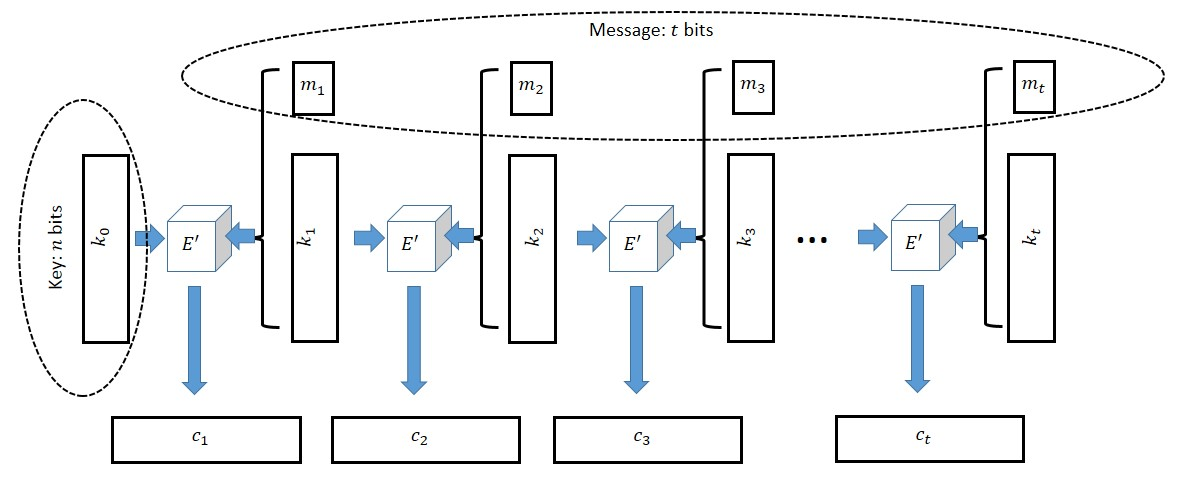
\includegraphics[width=\textwidth, height=0.25\paperheight, keepaspectratio]{../figure/length-extension.jpg}
\caption{Constructing a cipher with \(t\) bit long messages from one
with \(n+1\) long messages}
\label{cipherlengthextensionfig}
\end{figure}

\begin{pause} \label[pause]{2-This-is-perhaps-our-fi}

This is perhaps our first example of a non trivial cryptographic
theorem, and the blueprint for this proof will be one that we will
follow time and again during this course. Please make sure you read this
proof carefully and follow the argument.

\end{pause}

\begin{proof}[Proof of \cref{lengthextendthm}] \label[proof]{2-The-construction-depic}

The construction, depicted in \cref{cipherlengthextensionfig}, is
actually quite natural and variants of it are used in practice for
\emph{stream ciphers}, which are ways to encrypt arbitrarily long
messages using a fixed size key. The idea is that we use a key \(k_0\)
of size \(n\) to encrypt \textbf{(1)} a fresh key \(k_1\) of size \(n\)
and \textbf{(2)} one bit of the message. Now we can encrypt \(k_2\)
using \(k_1\) and so on and so forth. We now describe the construction
and analysis in detail.

Let \(t=t(n)\). We are given a cipher \(E'\) which can encrypt
\(n+1\)-bit long messages with an \(n\)-bit long key and we need to
encrypt a \(t\)-bit long message \(m=(m_1,\ldots,m_t) \in {\{0,1\}}^t\).
Our idea is simple (at least in hindsight). Let
\(k_0 {\leftarrow_{\tiny R}}{\{0,1\}}^n\) be our key (which is chosen at
random). To encrypt \(m\) using \(k_0\), the encryption function will
choose \(t\) random strings
\(k_1,\ldots, k_t {\leftarrow_{\tiny R}}{\{0,1\}}^n\). We will then
encrypt the \(n+1\)-bit long message \((k_1,m_1)\) with the key \(k_0\)
to obtain the ciphertext \(c_1\), then encrypt the \(n+1\)-bit long
message \((k_2,m_2)\) with the key \(k_1\) to obtain the ciphertext
\(c_2\), and so on and so forth until we encrypt the message
\((k_t,m_t)\) with the key \(k_{t-1}\).\footnote{The keys
  \(k_1,\ldots,k_t\) are sometimes known as \emph{ephemeral keys} in the
  crypto literature, since they are created only for the purposes of
  this particular interaction.} We output \((c_1,\ldots,c_t)\) as the
final ciphertext.\footnote{The astute reader might note that the key
  \(k_t\) is actually not used anywhere in the encryption nor decryption
  and hence we could encrypt \(n\) more bits of the message instead in
  this final round. We used the current description for the sake of
  symmetry and simplicity of exposition.}

To decrypt \((c_1,\ldots,c_t)\) using the key \(k_0\), first decrypt
\(c_1\) to learn \((k_1,m_1)\), then use \(k_1\) to decrypt \(c_2\) to
learn \((k_2,m_2)\), and so on until we use \(k_{t-1}\) to decrypt
\(c_t\) and learn \((k_t,m_t)\). Finally we can simply output
\((m_1,\ldots,m_t)\).

The above are clearly valid encryption and decryption algorithms, and
hence the real question becomes \emph{is it secure??}. The intuition is
that \(c_1\) hides all information about \((k_1,m_1)\) and so in
particular the first bit of the message is encrypted securely, and
\(k_1\) still can be treated as an unknown random string even to an
adversary that saw \(c_1\). Thus, we can think of \(k_1\) as a random
secret key for the encryption \(c_2\), and hence the second bit of the
message is encrypted securely, and so on and so forth.

Our discussion above looks like a reasonable intuitive argument, but to
make sure it's true we need to give an actual proof. Let
\(m,m' \in {\{0,1\}}^t\) be two messages. We need to show that
\(E_{U_n}(m) \approx E_{U_n}(m')\). The heart of the proof will be the
following claim:

\textbf{Claim:} Let \(\hat{E}\) be the algorithm that on input a message
\(m\) and key \(k_0\) works like \(E\) except that its \(i^{th}\) block
contains \(E'_{k_{i-1}}(k'_i,m_i)\) where \(k'_i\) is a \emph{random}
string in \({\{0,1\}}^n\), that is chosen \emph{independently} of
everything else including the key \(k_i\). Then, for every message
\(m\in{\{0,1\}}^t\)

\[
E_{U_n}(m) \approx \hat{E}_{U_n}(m)  \label{lengthextendclaimeq} \;.
\]

Note that \(\hat{E}\) is not a valid encryption scheme since it's not at
all clear there is a decryption algorithm for it. It is just an
hypothetical tool we use for the proof. Since both \(E\) and \(\hat{E}\)
are randomized encryption schemes (with \(E\) using \((t-1)n\) bits of
randomness for the ephemeral keys \(k_1,\ldots,k_{t-1}\) and \(\hat{E}\)
using \((2t-1)n\) bits of randomness for the ephemeral keys
\(k_1,\ldots,k_t,k'_2,\ldots,k'_t\)), we can also write
\eqref{lengthextendclaimeq} as
\begin{equation*}
E_{U_n}(m; U'_{tn}) \approx \hat{E}_{U_n}(m; U'_{(2t-1)n})
\end{equation*}
where we use \(U'_\ell\) to denote a random variable that is chosen
uniformly at random from \(\{0,1\}^\ell\) and independently from the
choice of \(U_n\) (which is chosen uniformly at random from
\(\{0,1\}^n\)).

Once we prove the claim then we are done since we know that for every
pair of messages \(m,m'\), \(E_{U_n}(m) \approx \hat{E}_{U_n}(m)\) and
\(E_{U_n}(m') \approx \hat{E}_{U_n}(m')\) but
\(\hat{E}_{U_n}(m) \approx \hat{E}_{U_n}(m')\) since \(\hat{E}\) is
essentially the same as the \(t\)-times repetition scheme we analyzed
above. Thus by the triangle inequality we can conclude that
\(E_{U_n}(m) \approx E_{U_n}(m')\) as we desired.

\textbf{Proof of claim:} We prove the claim by the hybrid method. For
\(j\in \{0,\ldots, t\}\), let \(H_j\) be the distribution of ciphertexts
where in the first \(j\) blocks we act like \(\hat{E}\) and in the last
\(t-j\) blocks we act like \(E\). That is, we choose
\(k_0,\ldots,k_t,k'_1,\ldots,k'_t\) independently at random from \(U_n\)
and the \(i^{th}\) block of \(H_j\) is equal to
\(E'_{k_{i-1}}(k_i,m_i)\) if \(i>j\) and is equal to
\(E'_{k_{i-1}}(k'_i,m_i)\) if \(i\leq j\). Clearly,
\(H_t = \hat{E}_{U_n}(m)\) and \(H_0 = E_{U_n}(m)\) and so it suffices
to prove that for every \(j\), \(H_{j-1} \approx H_j\). Indeed, let
\(j \in \{1,\ldots,t\}\) and suppose towards the sake of contradiction
that there exists an efficient \(Eve'\) such that

\begin{equation*}
\left| {\mathbb{E}}[ Eve'(H_{j-1})] - {\mathbb{E}}[ Eve'(H_j)]\right|\geq \epsilon \;\;(*)
\end{equation*}

where \(\epsilon = \epsilon(n)\) is noticeable. By the averaging
principle, there exists some fixed choice for
\(k'_1,\ldots,k'_t,k_0,\ldots,k_{j-2},k_j,\ldots,k_t\) such that \((*)\)
still holds. Note that in this case the only randomness is the choice of
\(k_{j-1}{\leftarrow_{\tiny R}}U_n\) and moreover the first \(j-1\)
blocks and the last \(t-j\) blocks of \(H_{j-1}\) and \(H_j\) would be
identical and we can denote them by \(\alpha\) and \(\beta\)
respectively and hence write \((*)\) as

\begin{equation*}
\left| {\mathbb{E}}_{k_{j-1}}[ Eve'(\alpha,E'_{k_{j-1}}(k_j,m_j),\beta) - Eve'(\alpha,E'_{k_{j-1}}(k'_j,m_j),\beta) ] \right| \geq \epsilon \;\;(**)
\end{equation*}

But now consider the adversary \(Eve\) that is defined as
\(Eve(c) = Eve'(\alpha,c,\beta)\). Then \(Eve\) is also efficient and by
\((**)\) it can distinguish between \(E'_{U_n}(k_j,m_j)\) and
\(E'_{U_n}(k'_j,m_j)\) thus contradicting the security of \((E',D')\).
This concludes the proof of the claim and hence the theorem.

\end{proof}

\subsection{Appendix: The computational
model}\label{2-Appendix-The-computati}

For concreteness sake let us give a precise definition of what it means
for a function or probabilistic process \(f\) mapping \(\{0,1\}^n\) to
\(\{0,1\}^m\) to be computable using \(T\) operations.

\begin{itemize}
\item
  If you have taken any course on computational complexity (such as
  Harvard CS 121), then this is the model of Boolean circuits, except
  that we also allow randomization.
\item
  If you have not taken such a course, you might simply take it on faith
  that it is possible to model what it means for an algorithm to be able
  to map an input \(x\) into an output \(f(x)\) using \(T\) ``elementary
  operations''.
\end{itemize}

In both cases you might want to skip this appendix and only return to it
if you find something confusing.

The model we use is a Boolean circuit that also has a
\(\ensuremath{\mathit{RAND}}\) gate that outputs a random bit. We could
use as the basic set of gates the standard
\(\ensuremath{\mathit{AND}}\), \(\ensuremath{\mathit{OR}}\) and
\(\ensuremath{\mathit{NOT}}\) but for simplicity we use the one-element
set \(\ensuremath{\mathit{NAND}}\). We represent the circuit as a
straightline program, but this is of course just a matter of
convenience. As shown (for example) in the \href{http://introtcs.org}{CS
121 textbook}, these two representations are identical.

\hypertarget{randprogdef}{}
\begin{definition}[Probabilistic straightline program] \label[definition]{randprogdef}

A \emph{probabilistic straightline program} consists of a sequence of
lines, each one of them one of the following forms:

\begin{itemize}
\item
  \texttt{foo = NAND(bar, baz)} where
  \texttt{foo},\texttt{bar},\texttt{baz} are variable identifiers.
\item
  \texttt{foo = RAND()} where \texttt{foo} is a variable identifier.
\end{itemize}

\end{definition}

Given a program \(\pi\), we say that its \emph{size} is the number of
lines it contains. Variables of the form \texttt{X[}\(i\)\texttt{]} or
\texttt{Y[}\(j\)\texttt{]} are considered input and output variables
respectively. If the input variables range from \(0\) to \(n-1\) and the
output variables range from \(0\) to \(m-1\) then the program computes
the probabilistic process that maps \(\{0,1\}^n\) to \(\{0,1\}^m\) in
the natural way. If \(F\) is a (probabilistic or deterministic) map of
\(\{0,1\}^n\) to \(\{0,1\}^m\), the \emph{complexity} of \(F\) is the
size of the smallest program \(P\) that computes it.

If you haven't taken a class such as CS121 before, you might wonder how
such a simple model captures complicated programs that use loops,
conditionals, and more complex data types than simply a bit in
\(\{0,1\}\), not to mention some special purpose crypto-breaking devices
that might involve tailor-made hardware. It turns out that it does (for
the same reason we can compile complicated programming languages to run
on silicon chips with a very limited instruction set). In fact, as far
as we know, this model can capture even computations that happen in
nature, whether it's in a bee colony or the human brain (which contains
about \(10^{10}\) neurons, so should in principle be simulatable by a
program that has up to a few order of magnitudes of the same number of
lines). Crucially, for cryptography, we care about such programs not
because we want to actually run them, but because we want to argue about
their \emph{non existence}. If we have a process that cannot be computed
by a straightline program of length shorter than \(2^{128}>10^{38}\)
then it seems safe to say that a computer the size of the human brain
(or even all the human and nonhuman brains on this planet) will not be
able to perform it either.

\paragraph{Advanced note: non uniformity.} The computational model we
use in this class is
\href{https://introtcs.org/public/lec_11_running_time.html\#nonuniformcompsec}{\emph{non
uniform}} (corresponding to Boolean circuits) as opposed to
\emph{uniform} (corresponding to Turing machines). If this distinction
doesn't mean anything to you, you can ignore it as it won't play a
significant role in what we do next. It basically means that we do allow
our programs to have hardwired constants of \(poly(n)\) bits where \(n\)
is the input/key length. In fact, to be precise, we will hold ourselves
to a higher standard than our adversary, in the sense that we require
our algorithms to be efficient in the stronger sense of being computable
in uniform probabilistic polynomial time (for some fixed polynomial,
often \(O(n)\) or \(O(n^2\))), while the adversary is allowed to use non
uniformity.

\paragraph{Quantum computing.} An interesting potential exception to
this principle that every natural process should be simulatable by a
straightline program of comparable complexity are processes where the
quantum mechanical notions of \emph{interference} and
\emph{entanglement} play a significant role. We will talk about this
notion of \emph{quantum computing} towards the end of the course, though
note that much of what we say does not really change when we add quantum
into the picture. As discussed in
\href{https://introtcs.org/public/lec_26_quantum_computing.html}{the CS
121 text}, we can still capture these processes by straightline programs
(that now have somewhat more complex form), and so most of what we'll do
just carries over in the same way to the quantum realm as long as we are
fine with conjecturing the strong form of the cipher conjecture, namely
that the cipher is infeasible to break even for quantum computers. All
current evidence points toward this strong form being true as well. The
field of constructing encryption schemes that are potentially secure
against quantum computers is known as
\href{https://en.wikipedia.org/wiki/Post-quantum_cryptography}{post
quantum cryptography} and we will return to this later in the course.

\chapter{Pseudorandomness}\label{3-Pseudorandomness}

\paragraph{Reading:} Katz-Lindell Section 3.3, Boneh-Shoup Chapter 3

Edited and expanded by Richard Xu in Spring 2020.

The nature of randomness has troubled philosophers, scientists,
statisticians and laypeople for many years.\footnote{Even lawyers
  grapple with this question, with a recent example being the debate of
  whether fantasy football is a game of chance or of skill.} Over the
years people have given different answers to the question of what does
it mean for data to be random, and what is the nature of probability.
The movements of the planets initially looked random and arbitrary, but
then early astronomers managed to find \emph{order} and make some
\emph{predictions} on them. Similarly, we have made great advances in
predicting the weather and will probably continue to do so.

So, while these days it seems as if the event of whether or not it will
rain a week from today is \emph{random}, we could imagine that in the
future we will be able to predict the weather accurately. Even the
canonical notion of a random experiment -tossing a coin -
\href{http://statweb.stanford.edu/~susan/papers/headswithJ.pdf}{might
not be as random as you'd think}: the second toss will have the same
result as the first one with about a 51\% chance. (Though
\href{https://www.stat.berkeley.edu/~aldous/Real-World/coin_tosses.html}{see
also this experiment}.) It is conceivable that at some point someone
would discover some function \(F\) that, given the first 100 coin tosses
by any given person, can predict the value of the
101\(^{th}\).\footnote{In fact such a function must exist in some sense
  since in the entire history of the world, presumably no sequence of
  \(100\) fair coin tosses has ever repeated.}

In all these examples, the physics underlying the event, whether it's
the planets' movement, the weather, or coin tosses, did not change but
only our powers to predict them. So to a large extent, \emph{randomness
is a function of the observer}, or in other words

\begin{quote}
\emph{If a quantity is hard to compute, it might as well be random.}
\end{quote}

Much of cryptography is about trying to make this intuition more formal,
and harnessing it to build secure systems. The basic object we want is
the following:

\hypertarget{prgdefconcrete}{}
\begin{definition}[Pseudorandom generator (concrete)] \label[definition]{prgdefconcrete}

A function \(G:{\{0,1\}}^n\rightarrow{\{0,1\}}^\ell\) is a
\((T,\epsilon)\) \emph{pseudorandom generator} if
\(G(U_n) \approx_{T,\epsilon} U_\ell\) where \(U_t\) denotes the uniform
distribution on \({\{0,1\}}^t\).

\end{definition}

That is, \(G\) is a \((T,\epsilon)\) pseudorandom generators if no
circuit of at most \(T\) gates can distinguish with bias better than
\(\epsilon\) between the output of \(G\) (on a random input) and a
uniformly random string of the same length.

As we did for the case of encryption, we will typically use
\emph{asymptotic terms} to describe cryptographic pseudorandom
generator. We say that \(G\) is simply a pseudorandom generator if it is
\((p(n),1/p(n))\)-pseudorandom generator for every polynomial
\(p(\cdot)\). In other words, we define pseudorandom generators as
follows:

\hypertarget{prgdef}{}
\begin{definition}[Pseudorandom generator] \label[definition]{prgdef}

Let \(G:\{0,1\}^* \rightarrow \{0,1\}^*\) be some function computable in
polynomial time. We say that \(G\) is a \emph{pseudorandom generator}
with length function \(\ell:\N \rightarrow \N\) (where \(\ell(n)>n\)) if

\begin{itemize}
\item
  For every \(x\in \{0,1\}^*\), \(|G(x)| = \ell(|x|)\).
\item
  For every polynomial \(p(\cdot)\) and sufficiently large \(n\), the
  function \(G_n\) (the restriction of \(G\) to inputs of length \(n\))
  is a \((p(n),\tfrac{1}{p(n)})\) pseudorandom generator.
\end{itemize}

\end{definition}

Equivalently, \(G\) as above is a pseudorandom generator if the two
distributions \(G(U_n)\) and \(U_{\ell(n)}\) are \emph{computationally
indistinguishable}.

\begin{pause} \label[pause]{3-This-definition-as-is-}

This definition (as is often the case in cryptography) is a bit long, so
you want to take your time parsing it. In particular you should verify
that you understand why the condition \eqref{prgdefeq} is the same as
saying that for every polynomial \(p:\N \rightarrow \N\), if \(n\) is
sufficiently large, then for every circuit \(D\) of at most \(T\) gates
(or equivalently, for every straightline program \(D\) of at most \(T\)
lines):
\[\left| \Pr[D(G(U_n))=1] - \Pr[ D(U_\ell)=1] \right| < \tfrac{1}{p(n)} \label{prgdefeq}\]

\end{pause}

Note that the requirement that \(\ell>n\) is crucial to make this notion
non-trivial, as for \(\ell=n\) the function \(G(x)=x\) clearly satisfies
that \(G(U_n)\) is identical to (and hence in particular
indistinguishable from) the distribution \(U_n\). (Make sure that you
understand this last statement!) However, for \(\ell>n\) this is no
longer trivial at all. In particular, if we didn't restrict the running
time of \(Eve\) then no such pseudo-random generator would exist:

\hypertarget{breakprglem}{}
\begin{lemma} \label[lemma]{breakprglem}

Suppose that \(G:{\{0,1\}}^n\rightarrow{\{0,1\}}^{n+1}\). Then there
exists an (inefficient) algorithm
\(Eve:{\{0,1\}}^{n+1}\rightarrow{\{0,1\}}\) such that
\({\mathbb{E}}[ Eve(G(U_n)) ]=1\) but
\({\mathbb{E}}[ Eve(U_{n+1})] \leq 1/2\).

\end{lemma}

\begin{proof} \label[proof]{3-On-input-yinn-consider}

On input \(y\in{\{0,1\}}^{n+1}\), consider the algorithm \(Eve\) that
goes over all possible \(x\in{\{0,1\}}^n\) and will output \(1\) if and
only if \(y=G(x)\) for some \(x\). Clearly
\({\mathbb{E}}[ Eve(G(U_n)) ] =1\). However, the set
\(S =\{ G(x) : x\in {\{0,1\}}^n \}\) on which Eve outputs \(1\) has size
at most \(2^n\), and hence a random \(y{\leftarrow_{\tiny R}} U_{n+1}\)
will fall in \(S\) with probability at most \(1/2\).

\end{proof}

It is not hard to show that if \(P=\ensuremath{\mathit{NP}}\) then the
above algorithm Eve can be made efficient. In particular, at the moment
we do not know how to \emph{prove} the existence of pseudorandom
generators. Nevertheless we believe that pseudorandom generators exist
and hence we make the following conjecture:

\begin{quote}
\textbf{Conjecture (The PRG conjecture):} For every \(n\), there exists
a pseudorandom generator \(G\) mapping \(n\) bits to \(n+1\)
bits.\footnote{The name ``The PRG conjecture'' is non-standard. In the
  literature this is known as the conjecture of existence of
  pseudorandom generators. This is a weaker form of ``The Optimal PRG
  Conjecture'' presented in my \href{https://goo.gl/G7bU4M}{intro to
  theoretical CS lecture notes} since the PRG conjecture only posits the
  existence of pseudorandom generators with arbitrary polynomial blowup,
  as opposed to an exponential blowup posited in the optimal PRG
  conjecture.}
\end{quote}

As was the case for the cipher conjecture, and any other conjecture,
there are two natural questions regarding the PRG conjecture: why should
we believe it and why should we care. Fortunately, the answer to the
first question is simple: it is known that the cipher conjecture
\emph{implies} the PRG conjecture, and hence if we believe the former we
should believe the latter. (The proof is highly non-trivial and we may
not get to see it in this course.) As for the second question, we will
see that the PRG conjecture implies a great number of useful
cryptographic tools, including the cipher conjecture (i.e., the two
conjectures are in fact equivalent). We start by showing that once we
can get to an output that is one bit longer than the input, we can in
fact obtain any polynomial number of bits.

\hypertarget{lengthextendprgthm}{}
\begin{theorem}[Length Extension for PRG's] \label[theorem]{lengthextendprgthm}

Suppose that the PRG conjecture is true. Then for every polynomial
\(t(n)\), there exists a pseudorandom generator mapping \(n\) bits to
\(t(n)\) bits.

\end{theorem}

\begin{figure}
\centering
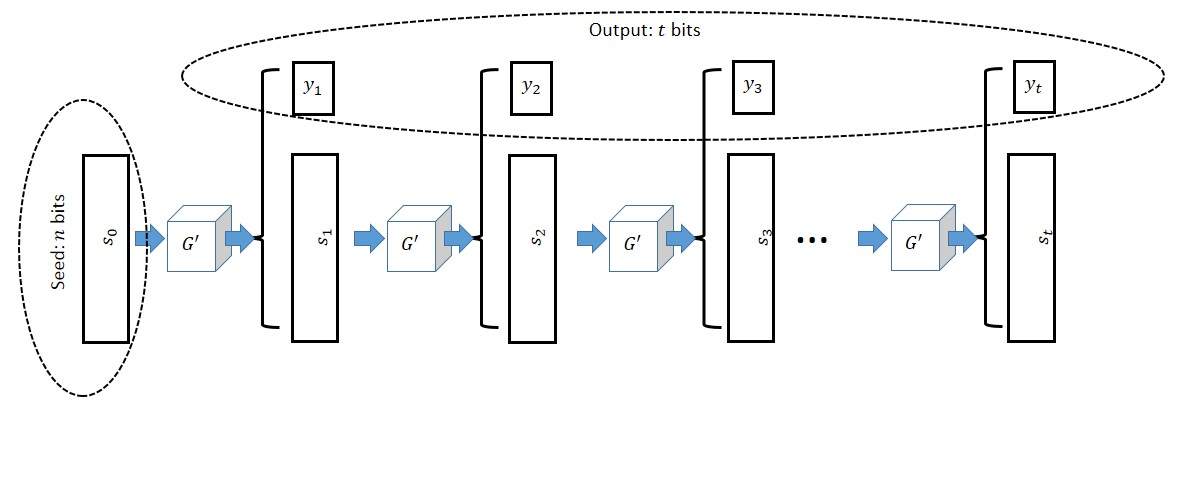
\includegraphics[width=\textwidth, height=0.25\paperheight, keepaspectratio]{../figure/length-extension-prg.jpg}
\caption{Length extension for pseudorandom generators}
\label{lengthextendprgfig}
\end{figure}

\begin{proof} \label[proof]{3-The-proof-of-this-theo}

The proof of this theorem is very similar to the length extension
theorem for ciphers, and in fact this theorem can be used to give an
alternative proof for the former theorem.

The construction is illustrated in \cref{lengthextendprgfig}. We are
given a pseudorandom generator \(G'\) mapping \(n\) bits into \(n+1\)
bits and need to construct a pseudorandom generator \(G\) mapping \(n\)
bits to \(t=t(n)\) bits for some polynomial \(t(\cdot)\). The idea is
that we maintain a state of \(n\) bits, which are originally our input
seed\footnote{Because we use a small input to grow a large pseudorandom
  string, the input to a pseudorandom generator is often known as its
  \emph{seed}.} \(s_0\), and at the \(i^{th}\) step we use \(G'\) to map
\(s_{i-1}\) to the \(n+1\)-long bit string \((s_i,y_i)\), output \(y_i\)
and keep \(s_i\) as our new state. To prove the security of this
construction we need to show that the distribution
\(G(U_n) = (y_1,\ldots,y_t)\) is computationally indistinguishable from
the uniform distribution \(U_t\). As usual, we will use the hybrid
argument. For \(i\in\{0,\ldots,t\}\) we define \(H_i\) to be the
distribution where the first \(i\) bits chosen at uniform, whereas the
last \(t-i\) bits are computed as above. Namely, we choose \(s_i\) at
random in \(\{0,1\}^n\) and continue the computation of
\(y_{i+1},\ldots,y_t\) from the state \(s_i\). Clearly \(H_0=G(U_n)\)
and \(H_t=U_t\) and hence by the triangle inequality it suffices to
prove that \(H_i \approx H_{i+1}\) for all \(i\in\{0,\ldots,t-1\}\). We
illustrate these two hybrids in \cref{lengthextendhybridfig}.

\begin{figure}
\centering
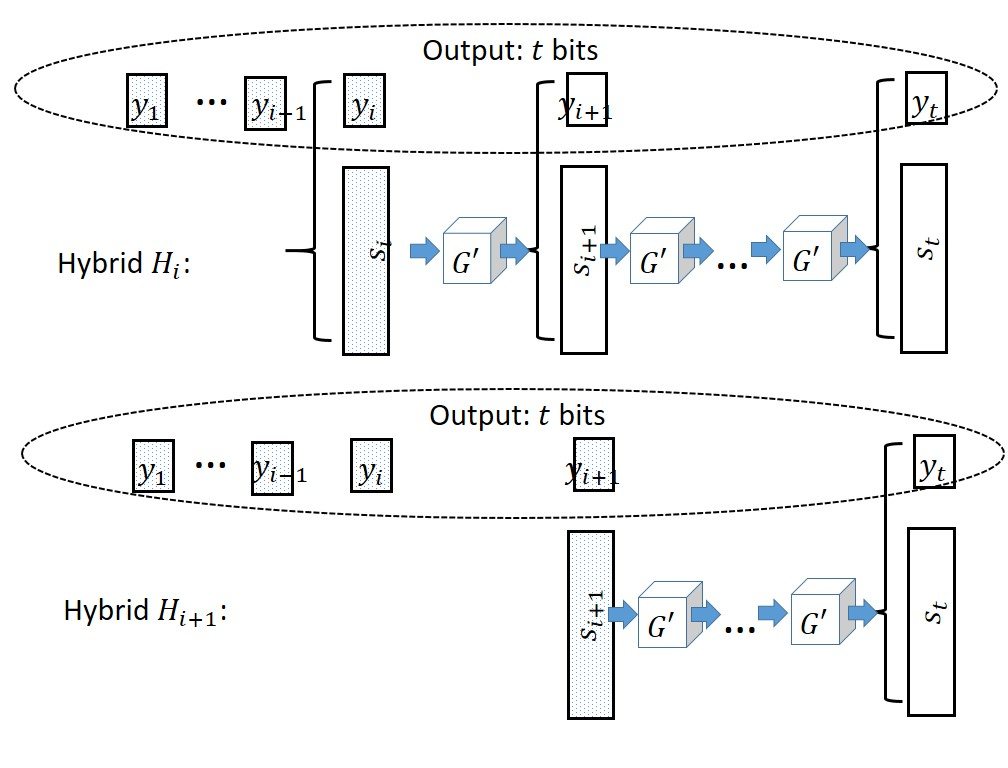
\includegraphics[width=\textwidth, height=0.25\paperheight, keepaspectratio]{../figure/length-extension-prg-hybrid.jpg}
\caption{Hybrids \(H_i\) and \(H_{i+1}\)--- dotted boxes refer to values
that are chosen independently and uniformly at random}
\label{lengthextendhybridfig}
\end{figure}

Now suppose otherwise, that there exists some adversary \(Eve\) such
that \(\left| \E[Eve(H_i)] - \E[Eve(H_{i+1})] \right| \geq \epsilon\)
for some non-negligible \(\epsilon\). We will build from \(Eve\) an
adversary \(Eve'\) breaking the security of the pseudorandom generator
\(G'\) (see \cref{reductionlengthextendfig}).

\begin{figure}
\centering
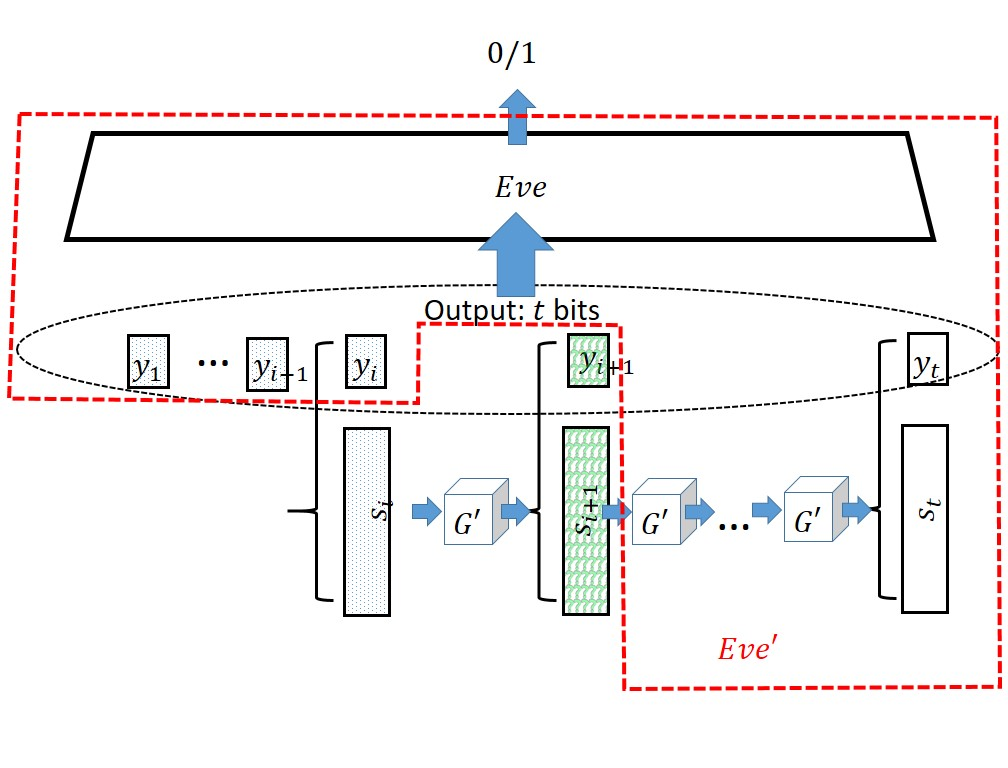
\includegraphics[width=\textwidth, height=0.25\paperheight, keepaspectratio]{../figure/length-extension-prg-adversary.jpg}
\caption{Building an adversary \(Eve'\) for \(G'\) from an adversary
\(Eve\) distinguishing \(H_i\) and \(H_{i+1}\). The boxes marked with
questions marks are those that are random or pseudorandom depending on
whether we are in \(H_i\) or \(H_{i+1}\). Everything inside the dashed
red lines is simulated by \(Eve'\) that gets as input the \(n+1\)-bit
string \((s_{i+1},y_{i+1})\).}
\label{reductionlengthextendfig}
\end{figure}

On input of string \(y\) of length \(n+1\), \(Eve'\) will interpret
\(y\) as \((s_{i+1},y_{i+1})\), choose \(y_1,\ldots,y_i\) randomly and
compute \(y_{i+2},\ldots,y_t\) as in our pseudorandom generator's
construction. \(Eve'\) will then feed \((y_1,\ldots,y_t)\) to \(Eve\)
and output whatever \(Eve\) does. Clearly, \(Eve'\) is efficient if
\(Eve\) is. Moreover, one can see that if \(y\) was random then \(Eve'\)
is feeding \(Eve\) with an input distributed according to \(H_{i+1}\)
while if \(y\) was of the form \(G(s)\) for a random \(s\) then \(Eve'\)
will feed \(Eve\) with an input distributed according to \(H_i\). Hence
we get that \(| \E[ Eve'(G'(U_n))] - \E[Eve'(U_{n+1})] | \geq \epsilon\)
contradicting the security of \(G'\).

\end{proof}

The proof of \cref{lengthextendprgthm} is indicative of many practical
constructions of pseudorandom generators. Many operating systems keep
track of an initial \emph{seed} of randomness, and supply a system call
\texttt{rand} that applies a pseudorandom generator \(G'\) to the
current seed, uses part of the output to update the seed, and returns
the remainder to the caller.

\subsection{Unpredictability: an alternative approach for proving the
length extension theorem}\label{3-Unpredictability-an-al}

The notion that being random is the same as being ``unpredictable'', as
discussed at the beginning of this chapter, can be formalized as
follows.

\hypertarget{unpreddef}{}
\begin{definition}[Unpredictable function] \label[definition]{unpreddef}

An efficiently computable function \(G:\{0,1\}^* \rightarrow \{0,1\}^*\)
is \emph{unpredictable} if, for any \(n\), \(1\le i<\ell(n)\) and
polynomially-sized circuit \(P\),
\begin{equation*}
\Pr_{y\leftarrow G(U_n)}[P(y_1,\ldots,y_{i-1}) = y_i] \le \frac12+negl(n).
\end{equation*}
Here, \(\ell(n)\) is the length function of \(G\) and
\(y\leftarrow G(U_n)\) denotes that \(y\) is a random output of \(G\).
In other words, no polynomial-sized circuit can predict the next bit of
the output of \(G\) given the previous bits significantly better than
guessing.

\end{definition}

We now show that the condition for a function \(G\) to be unpredictable
is equivalent to the condition for it to be a secure PRG. The proof is
detailed to give you another example of reduction proof.

\hypertarget{unpredequiv}{}
\begin{lemma} \label[lemma]{unpredequiv}

Let \(G:\{0,1\}^* \rightarrow \{0,1\}^*\) be a function with length
function \(\ell(n)\), then \(G\) is a secure PRG iff it is
unpredictable.

\end{lemma}

\begin{proof} \label[proof]{3-For-the-forward-direct}

For the forward direction, suppose for contradiction that there exists
some \(i\) and some circuit \(P\) can predict \(y_i\) given
\(y_1,\ldots,y_{i-1}\) with probability \(p\ge \frac12+\epsilon(n)\) for
non-negligible \(\epsilon\). Consider the adversary \(Eve\) that, given
a string \(y\), runs the circuit \(P\) on \(y_1,\ldots,y_{i-1}\), checks
if the output is equal to \(y_i\) and if so output 1.

If \(y=G(x)\) for a uniform \(x\), then \(P\) succeeds with probability
\(p\). If \(y\) is uniformly random, then we can imagine that the bit
\(y_i\) is generated \emph{after} \(P\) finished its calculation. The
bit \(y_i\) is \(0\) or \(1\) with equal probability, so \(P\) succeeds
with probability \(\frac12\). Since \(Eve\) outputs 1 when \(P\)
succeeds,
\begin{equation*}
\left| \Pr[Eve(G(U_n))=1] - \Pr[ Eve(U_\ell)=1] \right|=|p-\frac12|\ge \epsilon(n),
\end{equation*}
a contradiction.

For the backward direction, let \(G\) be an unpredictable function. Let
\(H_i\) be the distribution where the first \(i\) bits come from
\(G(U_n)\) while the last \(n-i\) bits are all random. Notice that
\(H_0=U_m\) and \(H_n=G(U_n)\), so it suffices to show that
\(H_{i-1}\cong H_{i}\) for all \(i\).

Suppose \(H_{i-1}\ncong H_{i}\) for some \(i\), i.e.~there exists some
\(Eve\) and non-negligible \(\epsilon\) such that
\begin{equation*}
\Pr[Eve(H_{i})=1]-\Pr[Eve(H_{i-1})=1]>\epsilon(n).
\end{equation*}
Consider the program \(P\) that, on input \((y_1,\ldots,y_{i-1})\),
picks the bit \(\hat y_{i},\ldots, \hat y_n\) uniformly at random. Then,
\(P\) calls \(Eve\) on the generated input. If \(Eve\) outputs \(1\)
then \(P\) outputs \(\hat y_{i}\), and otherwise it outputs
\(1-\hat y_{i}\).

The string \((y_1,\ldots,y_{i-1}, \hat y_i,\ldots,\hat y_n)\) has the
same distribution as \(H_{i-1}\). However, conditioned on
\(\hat y_i=y_i\), the string has distribution equal to \(H_{i}\). Let
\(p\) be the probability that \(Eve\) outputs \(1\) if \(\hat y_i=y_i\)
and \(q\) be the same probability when \(\hat y_i\neq y_i\), then we get
\begin{equation*}
p-\frac12(p+q)=\Pr[Eve(H_{i})=1]-\Pr[Eve(H_{i-1})=1]>\epsilon(n).
\end{equation*}
Therefore, the probability \(P\) outputs the correct value is equal to
\(\frac12p+\frac12(1-q)=\frac12+\epsilon(n)2\), a contradiction.

\end{proof}

The definition of unpredictability is useful because many of our
candidates for pseudorandom generators appeal to the unpredictability
definition in their proofs. For example, the Blum-Blum-Shub generator we
will see later in the chapter is proved to be unpredictable if the
``quadratic residuosity problem'' is hard. It is also nice to know that
our intuition at the beginning of the chapter can be formalized.

\section{Stream ciphers}\label{3-Stream-ciphers}

We now show a connection between psuedorandom generators and encryption
schemes:

\hypertarget{PRGandcipherthm}{}
\begin{theorem}[PRG conjecture implies Cipher conjectures] \label[theorem]{PRGandcipherthm}

If the PRG conjecture is true then so is the cipher conjecture.

\end{theorem}

It turns out that the converse direction is also true, and hence these
two conjectures are \emph{equivalent}. We will probably not show the
(quite non-trivial) proof of this fact in this course. (We might show
some weaker version of this harder direction.)

\begin{proof} \label[proof]{3-Recall-that-the-one-ti}

Recall that the \emph{one time pad} is a perfectly secure cipher but its
only problem was that to encrypt an \(n+1\) long message it needed an
\(n+1\) long bit key. Now using a pseudorandom generator, we can map an
\(n\)-bit long key into an \(n+1\)-bit long string that looks random
enough that we could use it as a key for the one-time pad. That is, our
cipher will look as follows:

\begin{equation*}
E_k(m) = G(k) \oplus m
\end{equation*}

and

\begin{equation*}
D_k(c) = G(k) \oplus c
\end{equation*}

Just like in the one time pad,
\(D_k(E_k(m)) = G(k) \oplus G(k) \oplus m = m\). Moreover, the
encryption and decryption algorithms are clearly efficient. We will
prove security of this encryption by showing the stronger claim that
\(E_{U_n}(m)\approx U_{n+1}\) for any \(m\).

Notice that \(U_{n+1}=U_{n+1}\oplus m\), as we showed in the security of
the one-time pad. Suppose that for some non-negligible
\(\epsilon=\epsilon(n)>0\) there is an efficient adversary \(Eve'\) such
that

\begin{equation*}
\left| {\mathbb{E}}[ Eve'(G(U_n)\oplus m)] - {\mathbb{E}}[ Eve'(U_{n+1}\oplus m) ] \right| \geq \epsilon.
\end{equation*}

Then the adversary \(Eve\) defined as \(Eve(y) = Eve'(y\oplus m)\) would
be also efficient. Furthermore, if \(y\) is pseudorandom then
\(Eve(y)=Eve'(G(U_n)\oplus m)\) and if \(y\) is uniformly random then
\(Eve'(U_{n+1}\oplus m)\). Then, \(Eve\) can distinguish the two
distributions with advantage \(\epsilon\), a contradiction.

\end{proof}

If the PRG outputs \(t(n)\) bits instead of \(n+1\) then we
automatically get an encryption scheme with \(t(n)\) long message
length. In fact, in practice if we use the length extension for PRG's,
we don't need to decide on the length of messages in advance. Every time
we need to encrypt another bit (or another block) \(m_i\) of the
message, we run the basic PRG to update our state and obtain some new
randomness \(y_i\) that we can XOR with the message and output. Such
constructions are known as \emph{stream ciphers} in the literature. In
much of the practical literature, the name \emph{stream cipher} is used
both for the pseudorandom generator itself as well as for the encryption
scheme that is obtained by combining it with the one-time pad.

\hypertarget{cointossingphonerm}{}
\begin{remark}[Using pseudorandom generators for coin tossing over the phone] \label[remark]{cointossingphonerm}

The following is a cute application of pseudorandom generators. Alice
and Bob want to toss a fair coin over the phone. They use a pseudorandom
generator \(G:\{0,1\}^n\rightarrow\{0,1\}^{3n}\).

\begin{itemize}
\tightlist
\item
  Alice will send \(z\leftarrow_R\{0,1\}^{3n}\) to Bob\\
\item
  Bob picks \(s\leftarrow_R\{0,1\}^n\) and with probability \(1/2\)
  sends \(G(s)\) (case I) and with probability \(1/2\) sends
  \(G(s)\oplus z\) (case II).\\
\item
  Alice then picks a random \(b\leftarrow_R\{0,1\}\) and sends it to
  Bob.\\
\item
  Bob reveals what he sent in the previous stage and if it was case I,
  their output is \(b\), and if it was case II, their output is \(1-b\).
\end{itemize}

It can be shown that (assuming the protocol is completed) the output is
a random coin, which neither Alice or Bob can control or predict with
more than negligible advantage over half. (Trying to formalize this and
prove it is an excellent exercise.)

\end{remark}

\section{What do pseudorandom generators actually look
like?}\label{3-What-do-pseudorandom-g}

So far we have made the conjectures that objects such as ciphers and
pseudorandom generators \emph{exist}, without giving any hint as to how
they would actually look like. (Though we have examples such as the
Caesar cipher, Vigenere, and Enigma of what secure ciphers \emph{don't}
look like.) As mentioned above, we do not know how to \emph{prove} that
any particular function is a pseudorandom generator. However, there are
quite simple \emph{candidates} (i.e., functions that are conjectured to
be secure pseudorandom generators), though care must be taken in
constructing them. We now consider candidates for functions that maps
\(n\) bits to \(n+1\) bits (or more generally \(n+c\) for some constant
\(c\) ) and look at least somewhat ``randomish''. As these constructions
are typically used as a basic component for obtaining a longer length
PRG via the length extension theorem (\cref{lengthextendprgthm}), we
will think of these pseudorandom generators as mapping a string
\(s\in\{0,1\}^n\) representing the current state into a string
\(s’\in\{0,1\}^n\) representing the new state as well as a string
\(b\in\{0,1\}^c\) representing the current output. See also Section 6.1
in Katz-Lindell and (for greater depth) Sections 3.6-3.9 in the
Boneh-Shoup book.

\subsection{Attempt 0: The counter
generator}\label{3-Attempt--The-counter-g}

To get started, let's look at an example of an obviously bogus
pseudorandom generator. We define the ``counter pseudorandom generator''
\(G:\{0,1\}^n \rightarrow \{0,1\}^{n+1}\) as follows. \(G(s)=(s',b)\)
where \(s' = s + 1 \mod 2^n\) (treating \(s\) and \(s'\) as numbers in
\(\{0,\ldots,2^n-1\}\)) and \(b\) is the least significant digit of
\(s'\). It's a great exercise to work out why this is \emph{not} a
secure pseudorandom generator.

\begin{pause} \label[pause]{3-You-should-really-paus}

You should really pause here and make sure you see why the ``counter
pseudorandom generator'' is not a secure pseudorandom generator. Show
that this is true even if we replace the least significant digit by the
\(k\)-th digit for every \(0 \leq k < n\).

\end{pause}

\subsection{Attempt 1: The linear checksum / linear feedback shift
register (LFSR)}\label{3-Attempt--The-linear-ch}

LFSR can be thought of as the ``mother'' (or maybe more like the sick
great-uncle) of all psuedorandom generators. One of the simplest ways to
generate a ``randomish'' extra digit given an \(n\) digit number is to
use a \emph{checksum} - some linear combination of the digits, with a
canonical example being the
\href{https://en.wikipedia.org/wiki/Cyclic_redundancy_check}{cyclic
redundancy check} or CRC.\footnote{CRC are often used to generate a
  ``control digit'' to detect mistypes of credit card or social security
  card number. This has very different goals than its use for
  pseudorandom generators, though there are some common intuitions
  behind the two usages.} This motivates the notion of a \emph{linear
feedback shift register generator} (LFSR): if the current state is
\(s\in\{0,1\}^n\) then the output is \(f(s)\) where \(f\) is a linear
function (modulo 2) and the new state is obtained by right shifting the
previous state and putting \(f(s)\) at the leftmost location. That is,
\(s'_1 = f(s)\) and \(s'_i = s_{i-1}\) for \(i\in\{2,\ldots,n\}\).

LFSR's have several good properties- if the function \(f(\cdot)\) is
chosen properly then they can have very long \emph{periods} (i.e., it
can take an exponential number of steps until the state repeats itself),
though that also holds for the simple ``counter'' generator we saw
above. They also have the property that every individual bit is equal to
\(0\) or \(1\) with probability exactly half (the counter generator also
shares this property).

A more interesting property is that (if the function is selected
properly) every two coordinates are independent from one another. That
is, there is some super-polynomial function \(t(n)\) (in fact \(t(n)\)
can be exponential in \(n\)) such that if
\(\ell \neq \ell' \in \{0,\ldots, t(n) \}\), then if we look at the two
random variables corresponding to the \(\ell\)-th and \(\ell'\)-th
output of the generator (where randomness is the initial state) then
they are distributed like two independent random coins. (This is
non-trivial to show, and depends on the choice of \(f\) - it is a
challenging but useful exercise to work this out.) The counter generator
fails badly at this condition: the least significant bits between two
consecutive states always flip.

There is a more general notion of a \emph{linear generator} where the
new state can be any invertible linear transformation of the previous
state. That is, we interpret the state \(s\) as an element of \(\Z_q^t\)
for some integers \(q,t\),\footnote{A ring is a set of elements where
  addition and multiplication are defined and obey the natural rules of
  associativity and commutativity (though without necessarily having a
  multiplicative inverse for every element). For every integer \(q\) we
  define \(\Z_q\) (known as the \emph{ring of integers modulo \(q\)}) to
  be the set \(\{0,\ldots,q-1\}\) where addition and multiplication is
  done modulo \(q\).} and let \(s’=F(s)\) and the output \(b=G(s)\)
where \(F:\Z_q^t\rightarrow\Z_q^t\) and \(G:\Z_q^t\rightarrow\Z_q\) are
invertible linear transformations (modulo \(q\)). This includes as a
special case the \emph{linear congruential generator} where \(t=1\) and
the map \(F(s)\) corresponds to taking \(as \pmod{q}\) where \(a\) is
number co-prime to \(q\).

All these generators are unfortunately insecure due to the great bane of
cryptography- the \emph{Gaussian elimination algorithm} which students
typically encounter in any linear algebra class.\footnote{Despite the
  name, the algorithm goes at least as far back as the Chinese
  \emph{Jiuzhang Suanshu} manuscript, circa 150 B.C.}

\hypertarget{gaussianelimthm}{}
\begin{theorem}[The unfortunate theorem for cryptography] \label[theorem]{gaussianelimthm}

There is a polynomial time algorithm to solve \(m\) linear equations in
\(n\) variables (or to certify no solution exists) over any ring.

\end{theorem}

Despite its seeming simplicity and ubiquity, Gaussian elimination (and
some generalizations and related algorithms such as Euclid's extended
g.c.d algorithm and the LLL lattice reduction algorithm) has been used
time and again to break candidate cryptographic constructions. In
particular, if we look at the first \(n\) outputs of a linear generator
\(b_1,\ldots,b_n\) then we can write linear equations in the unknown
initial state of the form \(f_1(s)=b_1,\ldots,f_n(s)=b_n\) where the
\(f_i\)'s are known linear functions. Either those functions are
\emph{linearly independent}, in which case we can solve the equations to
get the unique solution for the original state \(s\) and from which
point we can predict all outputs of the generator, or they are
dependent, which means that we can predict some of the outputs even
without recovering the original state. Either way, the generator is
\(*\sharp !\)'ed (where \(* \sharp !\) refers to whatever verb you
prefer to use when your system is broken). See also this
\href{http://alumni.cs.ucr.edu/~jsun/random-number.pdf}{1977 paper} of
James Reed.

\hypertarget{nocryptoprgs}{}
\begin{remark}[Non-cryptographic PRGs] \label[remark]{nocryptoprgs}

The above means that it is a bad idea to use a linear checksum as a
pseudorandom generator in a cryptographic application, and in fact in
any adversarial setting (e.g., one shouldn't hope that an attacker would
not be able to reverse engineer the algorithm\footnote{That number is
  obtained by applying an algorithm of \href{https://goo.gl/SL8ahM}{Hans
  Peter Luhn} which applies a simple map to each digit of the card and
  then sums them up modulo 10.} that computes the control digit of a
credit card number). However, that does not mean that there are no
legitimate cases where linear generators can be used . In a setting
where the application is not adversarial and you have an ability to
\emph{test} if the generator is actually successful, it might be
reasonable to use such insecure non-cryptographic generators. They tend
to be more efficient (though often not by much) and hence are often the
default option in many programming environments such as the
\texttt{C rand()} command. (In fact, the real bottleneck in using
cryptographic pseudorandom generators is often the generation of
\emph{entropy} for their seed, as discussed in the previous lecture, and
not their actual running time.)

\end{remark}

\subsection{From insecurity to security}\label{3-From-insecurity-to-sec}

It is often the case that we want to ``fix'' a broken cryptographic
primitive, such as a pseudorandom generator, to make it secure. At the
moment this is still more of an art than a science, but there are some
principles that cryptographers have used to try to make this more
principled. The main intuition is that there are certain properties of
computational problems that make them more amenable to algorithms (i.e.,
``easier'') and when we want to make the problems useful for
cryptography (i.e., ``hard'') we often seek variants that don't possess
these properties. The following table illustrates some examples of such
properties. (These are not formal statements, but rather is intended to
give some intuition )

\begin{longtable}[]{@{}ll@{}}
\toprule
Easy & Hard\tabularnewline
\midrule
\endhead
Continuous & Discrete\tabularnewline
Convex & Non-convex\tabularnewline
Linear & Non-linear (degree \(\geq 2\))\tabularnewline
Noiseless & Noisy\tabularnewline
Local & Global\tabularnewline
Shallow & Deep\tabularnewline
Low degree & High degree\tabularnewline
\bottomrule
\end{longtable}

Many cryptographic constructions can be thought of as trying to
transform an easy problem into a hard one by moving from the left to the
right column of this table.

The \textbf{discrete logarithm problem} is the discrete version of the
continuous real logarithm problem. The \textbf{learning with errors
problem} can be thought of as the noisy version of the linear equations
problem (or the discrete version of least squares minimization). When
constructing \textbf{block ciphers} we often have \emph{mixing}
transformation to ensure that the dependency structure between different
bits is \emph{global}, \emph{S-boxes} to ensure \emph{non-linearity},
and many \emph{rounds} to ensure \emph{deep} structure and \emph{large
algebraic degree}.

This also works in the other direction. Many algorithmic and machine
learning advances work by embedding a discrete problem in a continuous
convex one. Some attacks on cryptographic objects can be thought of as
trying to recover some of the structure (e.g., by embedding modular
arithmetic in the real line or ``linearizing'' non linear equations).

\subsection{Attempt 2: Linear Congruential Generators with dropped
bits}\label{3-Attempt--Linear-Congru}

One approach that is widely used in implementations of pseudorandom
generators is to take a linear generator such as the linear congruential
generators described above, and use for the output a ``chopped'' version
of the linear function and drop some of the least significant bits. The
operation of dropping these bits is non-linear and hence the attack
above does not immediately apply. Nevertheless, it turns out this attack
can be generalized to handle this case, and hence even with dropped bits
Linear Congruential Generators are completely insecure and should be
used (if at all) only in applications such as simulations where there is
no adversary. Section 3.7.1 in the Boneh-Shoup book describes one attack
against such generators that uses the notion of \emph{lattice
algorithms} that we will encounter later in this course in very
different contexts.

\section{Successful examples}\label{3-Successful-examples}

Let's now describe some \emph{successful} (at least per current
knowledge) pseudorandom generators:

\subsection{Case Study 1: Subset Sum
Generator}\label{3-Case-Study--Subset-Sum}

Here is an extremely simple generator that is yet still
secure\footnote{Actually modern computers will be able to break this
  generator via brute force, but if the length and number of the
  constants were doubled (or perhaps quadrupled) this should be
  sufficiently secure, though longer to write down.} as far as we know.

\begin{code}
# seed is a list of 40 zero/one values
# output is a 48 bit integer
def subset_sum_gen(seed):
  modulo = 0x1000000
  constants = [  
     0x3D6EA1, 0x1E2795, 0xC802C6, 0xBF742A, 0x45FF31,  
     0x53A9D4, 0x927F9F, 0x70E09D, 0x56F00A, 0x78B494,  
     0x9122E7, 0xAFB10C, 0x18C2C8, 0x8FF050, 0x0239A3,  
     0x02E4E0, 0x779B76, 0x1C4FC2, 0x7C5150, 0x81E05E,  
     0x154647, 0xB80E68, 0xA042E5, 0xE20269, 0xD3B7F3,  
     0xCC5FB9, 0x0BFC55, 0x847AE0, 0x8CFDF8, 0xE304B7,  
     0x869ACE, 0xB4CDAB, 0xC8E31F, 0x00EDC7, 0xC50541,  
     0x0D6DDD, 0x695A2F, 0xA81062, 0x0123CA, 0xC6C5C3 ]

  # return the modular sum of the constants
  # corresponding to ones in the seed
  return reduce(lambda x,y: (x+y) % modulo,
                map(lambda a,b: a*b, constants,seed))
\end{code}

The seed to this generator is an array \texttt{seed} of 40 bits, with 40
hardwired constants each 48 bits long (these constants were generated at
random, but are fixed once and for all, and are not kept secret and
hence are not considered part of the secret random seed). The output is
simply
\begin{equation*}
\sum_{i=1}^{40} \texttt{seed}[i]\texttt{constants}[i] \pmod{2^{48}}
\end{equation*}
and hence expands the \(40\) bit input into a \(48\) bit output.

This generator is loosely motivated by the ``subset sum'' computational
problem, which is NP hard. However, since NP hardness is a \emph{worst
case} notion of complexity, it does not imply security for pseudorandom
generators, which requires hardness of an \emph{average case} variant.
To get some intuition for its security, we can work out why (given that
it seems to be linear) we cannot break it by simply using Gaussian
elimination.

\begin{pause} \label[pause]{3-This-is-an-excellent-p}

This is an excellent point for you to stop and try to answer this
question on your own.

\end{pause}

Given the known constants and known output, figuring out the set of
potential seeds can be thought of as solving a \emph{single} equation in
40 variables. However, this equation is clearly overdetermined, and will
have a solution regardless of whether the observed value is indeed an
output of the generator, or it is chosen uniformly at random.

More concretely, we can use linear-equation solving to compute (given
the known constants \(c_1,\ldots,c_{40} \in \Z_{2^{48}}\) and the output
\(y \in \Z_{2^{48}}\)) the linear subspace \(V\) of all vectors
\((s_1,\ldots,s_{40}) \in (\Z_{2^{48}})^{40}\) such that
\(\sum s_i c_i = y \pmod{2^{48}}\). But, regardless of whether \(y\) was
generated at random from \(\Z_{2^{48}}\), or \(y\) was generated as an
output of the generator, the subspace \(V\) will always have the same
dimension (specifically, since it is formed by a single linear equation
over \(40\) variables, the dimension will be \(39\).) To break the
generator we seem to need to be able to decide whether this linear
subspace \(V \subseteq (\Z_{2^{48}})^{40}\) contains a \emph{Boolean
vector} (i.e., a vector \(s\in \{0,1\}^n\)). Since the condition that a
vector is Boolean is not defined by linear equations, we cannot use
Gaussian elimination to break the generator. Generally, the task of
finding a vector with \emph{small} coefficients inside a discrete linear
subspace is closely related to a classical problem known as finding the
\href{https://goo.gl/WRNT9S}{shortest vector in a lattice}. (See also
the \href{https://goo.gl/KwZWhV}{short integer solution (SIS) problem}.)

\subsection{Case Study 2: RC4}\label{3-Case-Study--RC}

The following is another example of an extremely simple generator known
as RC4 (this stands for Rivest Cipher 4, as Ron Rivest invented this in
1987) and is still fairly widely used today.

\begin{code}
def RC4(P,i,j):
    i = (i + 1) % 256
    j = (j + P[i]) % 256
    P[i], P[j] = P[j], P[i]
    return (P,i,j,P[(P[i]+P[j]) % 256])
\end{code}

The function \texttt{RC4} takes as input the current state
\texttt{P,i,j} of the generator and returns the new state together with
a single output byte. The state of the generator consists of an array
\texttt{P} of 256 bytes, which can be thought of as a \emph{permutation}
of the numbers \(0,\ldots,255\) in the sense that we maintain the
invariant that \(\texttt{P}[i]\neq\texttt{P}[j]\) for every \(i\neq j\),
and two indices \(i,j \in \{0,\ldots,255\}\). We can consider the
initial state as the case where \texttt{P} is a completely random
permutation and \(i\) and \(j\) are initialized to zero, although to
save on initial seed size, typically RC4 uses some ``pseudorandom'' way
to generate \texttt{P} from a shorter seed as well.

RC4 has extremely efficient software implementations and hence has been
widely implemented. However, it has several issues with its security. In
particular it was shown by Mantin\footnote{I typically do not include
  references in these lecture notes, and leave them to the texts, but I
  make here an exception because Itsik Mantin was a close friend of mine
  in grad school.} and Shamir that the second bit of RC4 is \emph{not}
random, even if the initialization vector was random. This and other
issues led to a practical attack on the 802.11b WiFi protocol, see
Section 9.9 in Boneh-Shoup. The initial response to those attacks was to
suggest to drop the first 1024 bytes of the output, but by now the
attacks have been sufficiently extended that RC4 is simply not
considered a secure cipher anymore. The ciphers Salsa and ChaCha,
designed by Dan Bernstein, have a similar design to RC4, and are
considered secure and deployed in several standard protocols such as
TLS, SSH and QUIC, see Section 3.6 in Boneh-Shoup.

\section{Case Study 3: B.B.S.}\label{3-Case-Study--BBS}

B.B.S., which stands for the authors Blum, Blum and Shub, is a simple
generator constructed from a potentially hard problem in number theory.

Let \(n=pq\), where \(p,q\) are primes. Then, the set \(Q_n\) of
\emph{quadratic residues modulo \(n\)} is the set
\begin{equation*}
Q_n=\{x^2\mid \gcd(x,N)=1\}.
\end{equation*}
The definition extends the concept of ``perfect squares'' when we are
working with standard integers. Notice that each number in \(Q_n\) has
at least one square root. We will see later in the course that if
\(n=pq\) then these numbers will have \(4\) square roots.

The B.B.S. generator chooses \(n=pq\), where \(p,q\) are prime and
\(p,q\equiv 3\pmod{4}\). The second condition guarantees that for each
\(y\in Q_n\), exactly one of its square roots fall in \(Q_n\). It also
maintains an initial state \(x\in\{0,1\}^n\), initialized to the seed.

\begin{code}
def BBS(x):
    return (x * x % n, x % 2)
\end{code}

In other words, it calculates the least significant bit of \(x\) and
squares its internal state. The security of this generator is based on
the \emph{quadratic residuosity problem}, which asks, given a number
\(x\), whether \(x\in Q_n\). The number theory required takes a while to
develop. However, it is interesting and I recommend the reader to search
up this particular generator.

\section{Non-constructive existence of pseudorandom
generators}\label{3-Non-constructive-exist}

We now show that, if we don't insist on \emph{constructivity} of
pseudorandom generators, then there exists pseudorandom generators with
output that are \emph{exponentially larger} than the input length.

\hypertarget{prgexist}{}
\begin{lemma}[Existence of inefficient pseudorandom generators] \label[lemma]{prgexist}

There is some absolute constant \(C\) such that for every
\(\epsilon,T\), if \(\ell > C (\log T + \log (1/\epsilon))\) and
\(m \leq T\), then there is an \((T,\epsilon)\) pseudorandom generator
\(G: \{0,1\}^\ell \rightarrow \{0,1\}^m\).

\end{lemma}

\begin{proofidea} \label[proofidea]{3-The-proof-uses-an-extr}

The proof uses an extremely useful technique known as the
``probabilistic method'' which is not too hard mathematically but can be
confusing at first.\footnote{There is a whole (highly recommended)
  \href{https://www.amazon.com/Probabilistic-Method-Discrete-Mathematics-Optimization/dp/1119061954/ref=dp_ob_title_bk}{book
  by Alon and Spencer} devoted to this method.} The idea is to give a
``non constructive'' proof of existence of the pseudorandom generator
\(G\) by showing that if \(G\) was chosen at random, then the
probability that it would be a valid \((T,\epsilon)\) pseudorandom
generator is positive. In particular this means that there \emph{exists}
a single \(G\) that is a valid \((T,\epsilon)\) pseudorandom generator.
The probabilistic method is just a \emph{proof technique} to demonstrate
the existence of such a function. Ultimately, our goal is to show the
existence of a \emph{deterministic} function \(G\) that satisfies the
conditions of a \((T, \epsilon)\) PRG.

\end{proofidea}

The above discussion might be rather abstract at this point, but would
become clearer after seeing the proof.

\begin{proof}[Proof of \cref{prgexist}] \label[proof]{3-Let-epsilonTellm-be-as}

Let \(\epsilon,T,\ell,m\) be as in the lemma's statement. We need to
show that there exists a function
\(G:\{0,1\}^\ell \rightarrow \{0,1\}^m\) that ``fools'' every \(T\) line
program \(P\) in the sense of \eqref{prgdefeq}. We will show that this
follows from the following claim:

\textbf{Claim I:} For every fixed NAND program / Boolean circuit \(P\),
if we pick \(G:\{0,1\}^\ell \rightarrow \{0,1\}^m\) \emph{at random}
then the probability that \eqref{prgdefeq} is violated is at most
\(2^{-T^2}\).

Before proving Claim I, let us see why it implies \cref{prgexist}. We
can identify a function \(G:\{0,1\}^\ell \rightarrow \{0,1\}^m\) with
its ``truth table'' or simply the list of evaluations on all its
possible \(2^\ell\) inputs. Since each output is an \(m\) bit string, we
can also think of \(G\) as a string in \(\{0,1\}^{m\cdot 2^\ell}\). We
define \(\mathcal{G}^m_\ell\) to be the set of all functions from
\(\{0,1\}^\ell\) to \(\{0,1\}^\ell\). As discussed above we can identify
\(\mathcal{F}_\ell^m\) with \(\{0,1\}^{m\cdot 2^\ell}\) and choosing a
random function \(G \sim \mathcal{F}_\ell^m\) corresponds to choosing a
random \(m\cdot 2^\ell\)-long bit string.

For every NAND program / Boolean circuit \(P\) let \(B_P\) be the event
that, if we choose \(G\) at random from \(\mathcal{F}_\ell^m\) then
\eqref{prgdefeq} is violated with respect to the program \(P\). It is
important to understand what is the sample space that the event \(B_P\)
is defined over, namely this event depends on the choice of \(G\) and so
\(B_P\) is a subset of \(\mathcal{F}_\ell^m\). An equivalent way to
define the event \(B_P\) is that it is the subset of all functions
mapping \(\{0,1\}^\ell\) to \(\{0,1\}^m\) that violate \eqref{prgdefeq},
or in other words: \[
B_P = \left\{ G \in \mathcal{F}_\ell^m \; \big| \; \left| \tfrac{1}{2^\ell}\sum_{s\in \{0,1\}^\ell} P(G(s)) - \tfrac{1}{2^m}\sum_{r \in \{0,1\}^m}P(r) \right| > \epsilon \right\} \;\;. \label{eq:eventdefine}
\] (We've replaced here the probability statements in \eqref{prgdefeq}
with the equivalent sums so as to reduce confusion as to what is the
sample space that \(B_P\) is defined over.)

To understand this proof it is crucial that you pause here and see how
the definition of \(B_P\) above corresponds to \eqref{eq:eventdefine}.
This may well take re-reading the above text once or twice, but it is a
good exercise at parsing probabilistic statements and learning how to
identify the \emph{sample space} that these statements correspond to.

Now, the number of programs of size \(T\) (or circuits of size \(T\)) is
at most \(2^{O(T\log T)}\). Since \(T\log T = o(T^2\)) this means that
if Claim I is true, then by the union bound it holds that the
probability of the union of \(B_P\) over \emph{all} NAND programs of at
most \(T\) lines is at most \(2^{O(T\log T)}2^{-T^2} < 0.1\) for
sufficiently large \(T\). What is important for us about the number
\(0.1\) is that it is smaller than \(1\). In particular this means that
there \emph{exists} a single \(G^* \in \mathcal{F}_\ell^m\) such that
\(G^*\) \emph{does not} violate \eqref{prgdefeq} with respect to any
NAND program of at most \(T\) lines, but that precisely means that
\(G^*\) is a \((T,\epsilon)\) pseudorandom generator.

Hence, it suffices to prove Claim I to conclude the proof of
\cref{prgexist}. Choosing a random
\(G: \{0,1\}^\ell \rightarrow \{0,1\}^m\) amounts to choosing
\(L=2^\ell\) random strings \(y_0,\ldots,y_{L-1} \in \{0,1\}^m\) and
letting \(G(x)=y_x\) (identifying \(\{0,1\}^\ell\) and \([L]\) via the
binary representation). Hence the claim amounts to showing that for
every fixed function \(P:\{0,1\}^m \rightarrow \{0,1\}\), if
\(L > 2^{C (\log T + \log \epsilon)}\) (which by setting \(C>4\), we can
ensure is larger than \(10 T^2/\epsilon^2\)) then the probability that
\[
\left| \tfrac{1}{L}\sum_{i=0}^{L-1} P(y_s) - \Pr_{s \sim \{0,1\}^m}[P(s)=1] \right| > \epsilon \label{prgdefeqchernoff}
\] is at most \(2^{-T^2}\). \eqref{{prgdefeqchernoff}} follows directly
from the Chernoff bound. If we let for every \(i\in [L]\) the random
variable \(X_i\) denote \(P(y_i)\), then since \(y_0,\ldots,y_{L-1}\) is
chosen independently at random, these are independently and identically
distributed random variables with mean
\(\E_{y \sim \{0,1\}^m}[P(y)]= \Pr_{y\sim \{0,1\}^m}[ P(y)=1]\) and
hence the probability that they deviate from their expectation by
\(\epsilon\) is at most \(2\cdot 2^{-\epsilon^2 L/2}\).

\end{proof}

\chapter{Pseudorandom functions}\label{Pseudorandom-functions}

In the last lecture we saw the notion of \emph{pseudorandom generators},
and introduced the \textbf{PRG conjecture}, which stated that there
exists a pseudorandom generator mapping \(n\) bits to \(n+1\) bits. We
have seen the \emph{length extension} theorem, which states that given
such a pseudorandom generator, there exists a generator mapping \(n\)
bits to \(m\) bits for an arbitrarily large polynomial \(m(n)\). But can
we extend it even further? Say, to \(2^n\) bits? Does this question even
make sense? And why would we want to do that? This is the topic of this
lecture.

At a first look, the notion of extending the output length of a
pseudorandom generator to \(2^n\) bits seems nonsensical. After all, we
want our generator to be \emph{efficient} and just writing down the
output will take exponential time. However, there is a way around this
conundrum. While we can't efficiently write down the full output, we can
require that it would be possible, given an index
\(i\in \{0,\ldots,2^n-1\}\), to compute the \(i^{th}\) bit of the output
in polynomial time.\footnote{In this course we will often index strings
  and numbers starting from zero rather than one, and so typically index
  the coordinates of a string \(y\in \{0,1\}^N\) as \(0,\ldots,N-1\)
  rather than \(1,\ldots,N\). But we will not be religious about it and
  occasionally ``lapse'' into one-based indexing. In almost all cases,
  this makes no difference.} That is, we require that the function
\(i \mapsto G(s)_i\) is efficiently computable and (by security of the
pseudorandom generator) indistinguishable from a function that maps each
index \(i\) to an independent random bit in \(\{0,1\}\). This is the
notion of a \emph{pseudorandom function generator} which is a bit subtle
to define and construct, but turns out to have a great many applications
in cryptography.

\hypertarget{prfdef}{}
\begin{definition}[Pseudorandom Function Generator] \label[definition]{prfdef}

An efficiently computable function \(F\) taking two inputs
\(s\in\{0,1\}^n\) and \(i\in \{0,\ldots,2^n-1\}\) and outputting a
single bit \(F(s,i)\) is a \emph{pseudorandom function (PRF) generator}
if for every polynomial time adversary \(A\) outputting a single bit and
polynomial \(p(n)\), if \(n\) is large enough then:

\[ \left| \E_{s\in\{0,1\}^n}[ A^{F(s,\cdot)}(1^n)] - \E_{H \leftarrow_R [2^n]\rightarrow\{0,1\}}[A^H(1^n)] \right| < 1/p(n) \;.\]

\end{definition}

Some notes on notation are in order. The input \(1^n\) is simply a
string of \(n\) ones, and it is a typical cryptography convention to
assume that such an input is always given to the adversary. This is
simply because by ``polynomial time adversary'' we really mean
polynomial in \(n\) (which is our key size or security
parameter)\footnote{This also allows us to be consistent with the notion
  of ``polynomial in the size of the input.''}. The notation
\(A^{F(s,\cdot)}\) means that \(A\) has \emph{black box} (also known as
\emph{oracle}) access to the function that maps \(i\) to \(F(s,i)\).
That is, \(A\) can choose an index \(i\), query the box and get
\(F(s,i)\), then choose a new index \(i'\), query the box to get
\(F(s,i')\), and so on for a polynomial number of queries. The notation
\(H \leftarrow_R [2^n] \rightarrow \{0,1\}\) means that \(H\) is a
completely random function that maps every index \(i\) to an independent
and random different bit.

\hypertarget{randfuncs}{}
\begin{remark}[Completely Random Functions] \label[remark]{randfuncs}

This notion of a randomly chosen function can be difficult to wrap your
mind around. Try to imagine a table of all of the strings in
\(\{0, 1\}^n\). We now go to each possible input, randomly generate a
bit to be its output, and write down the result in the table. When we're
done, we have a length \(2^n\) lookup table that maps each input to an
output that was generated uniformly at random and independently of all
other outputs. This lookup table is now our random function \(H\).

In practice it's too cumbersome to actually generate all \(2^n\) bits,
and sometimes in theory it's convenient to think of each output as
generated only after a query is made. This leads to adopting the
\emph{lazy evaluation model}. In the lazy evaluation model, we imagine
that a lazy person is sitting in a room with the same lookup table as
before, but with all entries blank. If someone makes some query
\(H(s)\), the lazy person checks if the entry for \(s\) in the lookup
table is blank. If so, the lazy evaluator generates a random bit, writes
down the result for \(s\), and returns it. Otherwise, if an output has
already been generated for \(s\) previously (because \(s\) has been
queried before), the lazy evaluator simply returns this value. Can you
see why this model is more convenient in some ways?

One last way to think about how a completely random function is
determined is to first observe that there exist a total of \(2^{2^n}\)
functions from \(\{0, 1\}^n\) to \(\{0, 1\}\) (can you see why? It may
be easier to think of them as functions from \([2^n]\) to \(\{0, 1\}\)).
We choose one of them uniformly at random to be \(H\), and it's still
the case that for any given input \(s\) the result \(H(s)\) is \(0\) or
\(1\) with equal probability independent of any other input.

Regardless of which model we use to think about generating \(H\), after
we've chosen \(H\) and put it in a black box, the behavior of \(H\) is
in some sense ``deterministic'' because given the same query it will
always return the same result. However, before we ever make any given
query \(s\) we can only guess \(H(s)\) correctly with probability
\(\tfrac{1}{2}\), because without previously observing \(H(s)\) it is
effectively random and undecided to us (just like in the lazy evaluator
model).

\end{remark}

\begin{pause} \label[pause]{Now-would-be-a-fantastic-}

Now would be a fantastic time to stop and think deeply about the three
constructions in the remark above, and in particular why they are all
equivalent. If you don't feel like thinking then at the very least you
should make a mental note to come back later if you're confused, because
this idea will be very useful down the road.

\end{pause}

Thus, the notation \(A^H\) in the PRF definition means \(A\) has access
to a completely random black box that returns a random bit for any new
query made, and on previously seen queries returns the same bit as
before. Finally one last note: below we will identify the set
\([2^n] = \{0,\ldots,2^n-1\}\) with the set \(\{0,1\}^n\) (there is a
one to one mapping between those sets using the binary representation),
and so we will treat \(i\) interchangeably as a number in \([2^n]\) or a
string in \(\{0,1\}^n\).

Informally, if \(F\) is a pseudorandom function generator, then if we
choose a random string \(s\) and consider the function \(f_s\) defined
by \(f_s(i) = F(s,i)\), no efficient algorithm can distinguish between
black box access to \(f_s(\cdot)\) and black box access to a completely
random function (see \cref{prfmodelfig}). Notably, black box access
implies that a priori the adversary does not know which function it's
querying. From the adversary's point of view, they query some oracle
\(O\) (which behind the scenes is either \(f_s(\cdot)\) or \(H\)), and
must decide if \(O = f_s(\cdot)\) or \(O = H\). Thus often instead of
talking about a pseudorandom function generator we will refer to a
\emph{pseudorandom function collection} \(\{ f_s \}\) where by that we
mean the map \(F(s,i)=f_s(i)\) is a pseudorandom function generator.


\begin{figure}
\centering
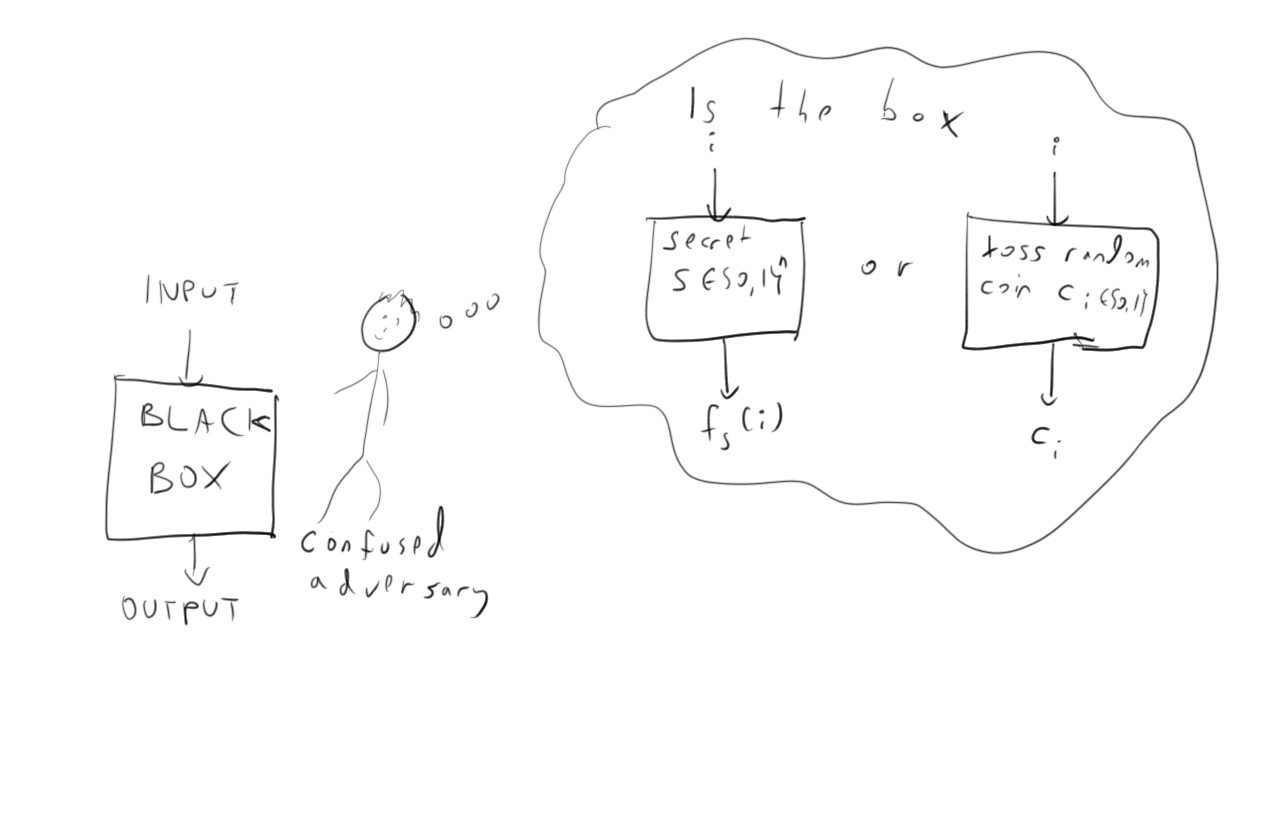
\includegraphics[width=\textwidth, height=0.25\paperheight, keepaspectratio]{../figure/pseudorandom_function.jpg}
\caption{In a pseudorandom function, an adversary cannot tell whether
they are given a black box that computes the function
\(i \mapsto F(s,i)\) for some secret \(s\) that was chosen at random and
fixed, or whether the black box computes a completely random function
that tosses a fresh random coin whenever it's given a new input \(i\).}
\label{prfmodelfig}
\end{figure}

In the next lecture we will see the proof of following theorem (due to
Goldreich, Goldwasser, and Micali)

\hypertarget{prffromprgthmone}{}
\begin{theorem}[PRFs from PRGs] \label[theorem]{prffromprgthmone}

Assuming the PRG conjecture, there exists a secure pseudorandom function
generator.

\end{theorem}

But before we see the proof of \cref{prffromprgthmone}, let us see why
pseudorandom functions could be useful.

\section{One time passwords (e.g.~Google Authenticator, RSA ID,
etc.)}\label{One-time-passwords-egGoog}

Until now we have talked about the task of \emph{encryption}, or
protecting the \emph{secrecy} of messages. But the task of
\emph{authentication}, or protecting the \emph{integrity} of messages is
no less important. For example, consider the case that you receive a
software update for your PC, phone, car, pacemaker, etc. over an open
channel such as an unencrypted Wi-Fi connection. The contents of that
update are not secret, but it is of crucial importance that it was
unchanged from the message sent out by the company and that no malicious
attacker had modified the code. Similarly, when you log into your bank,
you might be much more concerned about the possibility of someone
impersonating you and cleaning out your account than you are about the
secrecy of your information.

Let's start with a very simple scenario which we'll call \textbf{the
login problem}. \textbf{Alice} and \textbf{Bob} share a key as before,
but now Alice wants to simply prove her identity to Bob. What makes this
challenging is that this time they need to contend with not the passive
eavesdropping Eve but the active adversary \textbf{Mallory}, who
completely controls the communication channel between them and can
modify (or \emph{mall}) any message that they send. Specifically for the
identity proving case, we think of the following scenario. Each instance
of such an \textbf{identification protocol} consists of some interaction
between Alice and Bob that ends with Bob deciding whether to accept it
as authentic or reject as an impersonation attempt. Mallory's goal is to
fool Bob into accepting her as Alice.

The most basic way to try to solve the login problem is by simply using
a \emph{password}. That is, if we assume that Alice and Bob can share a
key, we can treat this key as some secret password \(p\) that was
selected at random from \(\{0,1\}^n\) (and hence can only be guessed
with probability \(2^{-n}\)). Why doesn't Alice simply send \(p\) to Bob
to prove to him her identity? A moment's thought shows that this would
be a very bad idea. Since Mallory is controlling the communication line,
she would learn \(p\) after the first identification attempt and could
then easily impersonate Alice in future interactions. However, we seem
to have just the tool to protect the secrecy of \(p\)---
\emph{encryption}. Suppose that Alice and Bob share a secret key \(k\)
and an additional secret password \(p\). Wouldn't a simple way to solve
the login problem be for Alice to send to Bob an encryption of the
password \(p\)? After all, the security of the encryption should
guarantee that Mallory can't learn \(p\), right?

\begin{pause} \label[pause]{This-would-be-a-good-time}

This would be a good time to stop reading and try to think for yourself
whether using a secure encryption to encrypt \(p\) would guarantee
security for the login problem. (No really, stop and think about it.)

\end{pause}

The problem is that Mallory does not have to learn the password \(p\) in
order to impersonate Alice. For example, she can simply record the
message Alice \(c_1\) sends to Bob in the first session and then
\emph{replay} it to Bob in the next session. Since the message is a
valid encryption of \(p\), then Bob would accept it from Mallory! (This
is known as a \emph{replay attack} and is a common attack one needs to
protect against in cryptographic protocols.) One can try to put in
countermeasures to defend against this particular attack, but its
existence demonstrates that secrecy of the password does not guarantee
security of the login protocol.

\subsection{How do pseudorandom functions help in the login
problem?}\label{How-do-pseudorandom-funct}

The idea is that they create what's known as a \emph{one time password}.
Alice and Bob will share an index \(s\in\{0,1\}^n\) for the pseudorandom
function generator \(\{ f_s \}\). When Alice wants to prove to Bob her
identity, Bob will choose a random \(i\leftarrow_R\{0,1\}^n\), and send
\(i\) to Alice, and then Alice will send
\(f_s(i),f_s(i+1),\ldots,f_s(i+\ell-1)\) to Bob where \(\ell\) is some
parameter (you can think of \(\ell=n\) for simplicity). Bob will check
that indeed \(y=f_s(i)\) and if so accept the session as authentic.

The formal protocol is as follows:

\paragraph{Protocol} \texttt{PRF-Login}\textbf{:}

\begin{itemize}
\tightlist
\item
  Shared input: \(s\in\{0,1\}^n\). Alice and Bob treat it as a seed for
  a pseudorandom function generator \(\{ f_s \}\).
\item
  In every session Alice and Bob do the following:

  \begin{enumerate}
  \def\labelenumi{\arabic{enumi}.}
  \tightlist
  \item
    Bob chooses a random \(i\leftarrow_R[2^n]\) and sends \(i\) to
    Alice.
  \item
    Alice sends \(y_1,\ldots,y_\ell\) to Bob where \(y_j = f_s(i+j-1)\).
  \item
    Bob checks that for every \(j\in\{1,\ldots,\ell\}\),
    \(y_j = f_s(i+j-1)\) and if so accepts the session; otherwise he
    rejects it.
  \end{enumerate}
\end{itemize}

As we will see it's not really crucial that the input \(i\) (which is
known in crypto parlance as a \emph{nonce}) is random. What is crucial
is that it never repeats itself, to foil a replay attack. For this
reason in many applications Alice and Bob compute \(i\) as a function of
the current time (for example, the index of the current minute based on
some agreed-upon starting point), and hence we can make it into a one
message protocol. Also the parameter \(\ell\) is sometimes chosen to be
deliberately short so that it will be easy for people to type the values
\(y_1,\ldots,y_\ell\).


\begin{marginfigure}
\centering
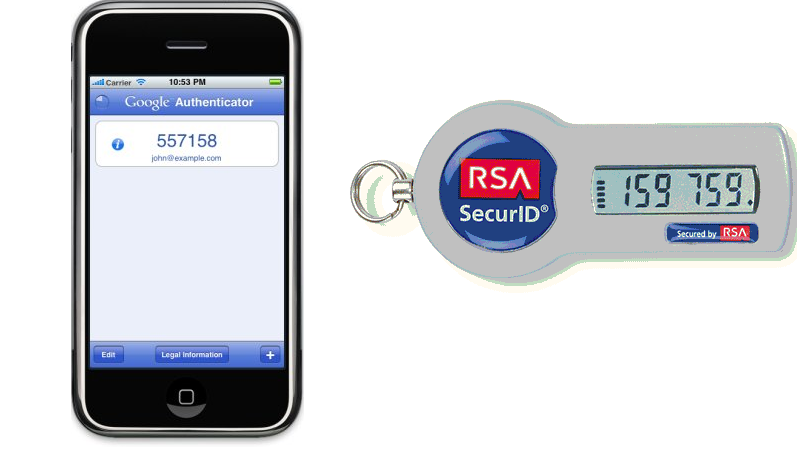
\includegraphics[width=\linewidth, height=1.5in, keepaspectratio]{../figure/google-authenticator.jpg}
\caption{The Google Authenticator app is one popular example of a
one-time password scheme using pseudorandom functions. Another example
is RSA's SecurID token.}
\label{tmplabelfig}
\end{marginfigure}

\emph{Why is this secure?} The key to understanding schemes using
pseudorandom functions is to imagine what would happen if instead of a
\emph{pseudo} random function, \(f_s\) would be an \emph{actual} random
function. In a truly random function, every one of the values
\(f_s(0),\ldots,f_s(2^n-1)\) is chosen independently and uniformly at
random from \(\{0,1\}\). One useful way to imagine this is using the
concept of ``lazy evaluation''. We can think of \(f_S\) as determined by
tossing \(2^n\) different coins for the values \(f(0),\ldots,f(2^n-1)\).
Now consider the case where we don't actually toss the \(i^{th}\) coin
until we need it. The crucial point is that if we have queried the
function in \(T\ll 2^n\) places, then when Bob chooses a random
\(i\in[2^n]\) it is \emph{extremely unlikely} that any one of the set
\(\{i,i+1,\ldots,i+\ell-1\}\) will be one of those locations that we
previously queried. Thus, if the function was truly random, Mallory has
\emph{no information} on the value of the function in these coordinates,
and would be able to predict (or rather, guess) it in all these
locations with probability at most \(2^{-\ell}\).

\begin{pause} \label[pause]{Please-make-sure-you-unde}

Please make sure you understand the informal reasoning above, since we
will now translate this into a formal theorem and proof.

\end{pause}

\hypertarget{loginprfthm}{}
\begin{theorem}[Login protocol via PRF] \label[theorem]{loginprfthm}

Suppose that \(\{ f_s \}\) is a secure pseudorandom function generator
and Alice and Bob interact using Protocol \texttt{PRF-Login} for some
polynomial number \(T\) of sessions (over a channel controlled by
Mallory). After observing these interactions, Mallory then interacts
with Bob, where Bob follows the protocol's instructions but Mallory has
access to arbitrary efficient computation. Then, the probability that
Bob accepts the interaction is at most \(2^{-\ell}+\mu(n)\) where
\(\mu(\cdot)\) is some negligible function.

\end{theorem}

\begin{proof} \label[proof]{This-proof-as-so-many-oth}

This proof, as so many others in this course, uses an argument via
contradiction. We assume, towards the sake of contradiction, that there
exists an adversary \(M\) (for Mallory) that can break the
identification scheme \texttt{PRF-Login} with probability
\(2^{-\ell}+\epsilon\) after \(T\) interactions. We then construct an
attacker \(A\) that can distinguish access to \(\{ f_s \}\) from access
to a random function in \(poly(T)\) time and with bias at least
\(\epsilon/2\).

How do we construct this adversary \(A\)? The idea is as follows. First,
we prove that if we ran the protocol \texttt{PRF-Login} using an
\emph{actual random} function, then \(M\) would not be able to succeed
in impersonating with probability better than \(2^{-\ell}+negligible\).
Therefore, if \(M\) does do better, then we can use that to distinguish
\(f_s\) from a random function. The adversary \(A\) gets some black box
\(O(\cdot)\) (for \emph{oracle}) and will use it while internally
simulating all the parties--- Alice, Bob and Mallory (using \(M\)) in
the \(T+1\) interactions of the \texttt{PRF-Login} protocol. Whenever
any of the parties needs to evaluate \(f_s(i)\), \(A\) will forward
\(i\) to its black box \(O(\cdot)\) and return the value \(O(i)\). It
will then output \(1\) if an only if \(M\) succeeds in impersonation in
this internal simulation. The argument above showed that if \(O(\cdot)\)
is a truly random function, then the probability that \(A\) outputs
\(1\) is at most \(2^{-\ell}+negligible\) (and so in particular less
than \(2^{-\ell}+\epsilon/2\)). On the other hand, if \(O(\cdot)\) is
the function \(i \mapsto f_s(i)\) for some fixed and random \(s\), then
this probability is at least \(2^{-\ell}+\epsilon\). Thus \(A\) will
distinguish between the two cases with bias at least \(\epsilon/2\). We
now turn to the formal proof:

\textbf{Claim 1:} Let \texttt{PRF-Login*} be the hypothetical variant of
the protocol \texttt{PRF-Login} where Alice and Bob share a completely
random function \(H:[2^n]\rightarrow\{0,1\}\). Then, no matter what
Mallory does, the probability she can impersonate Alice after observing
\(T\) interactions is at most \(2^{-\ell}+(8\ell T)/2^n\).

(If \texttt{PRF-Login*} is easier to prove secure than
\texttt{PRF-Login}, you might wonder why we bother with
\texttt{PRF-Login} in the first place and not simply use
\texttt{PRF-Login*}. The reason is that specifying a random function
\(H\) requires specifying \(2^n\) bits, and so that would be a
\emph{huge} shared key. So \texttt{PRF-Login*} is not a protocol we can
actually run but rather a hypothetical ``mental experiment'' that helps
us in arguing about the security of \texttt{PRF-Login}.)

\textbf{Proof of Claim 1:} Let \(i_1,\ldots,i_{2T}\) be the nonces
chosen by Bob and recieved by Alice in the first \(T\) iterations. That
is, \(i_1\) is the nonce chosen by Bob in the first iteration while
\(i_2\) is the nonce that Alice received in the first iteration (if
Mallory doesn't modify it then \(i_1=i_2\)). Similarly, \(i_3\) is the
nonce chosen by Bob in the second iteration while \(i_4\) is the nonce
received by Alice and so on and so forth. Let \(i\) be the nonce chosen
in the \(T+1^{st}\) iteration in which Mallory tries to impersonate
Alice. We claim that the probability that there exists some
\(j\in\{1,\ldots,2T\}\) such that \(|i-i_j|<2\ell\) is at most
\(8\ell T/2^n\). Indeed, let \(S\) be the union of all the intervals of
the form \(\{ i_j-2\ell+1,\ldots, i_j+2\ell-1 \}\) for
\(1 \leq j \leq 2T\). Since it's a union of \(2T\) intervals each of
length less than \(4\ell\), \(S\) contains at most \(8T\ell\) elements,
so the probability that \(i\in S\) is \(|S|/2^n \leq (8T\ell)/2^n\).
Now, if there does \emph{not} exists a \(j\) such that \(|i-i_j|<2\ell\)
then it means in particular that all the queries to \(H(\cdot)\) made by
either Alice or Bob during the first \(T\) iterations are disjoint from
the interval \(\{ i,i+1,\ldots,i+\ell-1 \}\). Since \(H(\cdot)\) is a
completely random function, the values \(H(i),\ldots,H(i+\ell-1)\) are
chosen uniformly and independently from all the rest of the values of
this function. Since Mallory's message \(y\) to Bob in the \(T+1^{st}\)
iteration depends only on what she observed in the past, the values
\(H(i),\ldots,H(i+\ell-1)\) are \emph{independent} from \(y\), and hence
under this condition that there is no overlap between this interval and
prior queries, the probability that they equal \(y\) is \(2^{-\ell}\).
QED (Claim 1).

The proof of Claim 1 is not hard but it is somewhat subtle, so it's good
to go over it again and make sure you understand it.

Now that we have Claim 1, the proof of the theorem follows as outlined
above. We build an adversary \(A\) to the pseudorandom function
generator from \(M\) by having \(A\) simulate ``inside its belly'' all
the parties Alice, Bob and Mallory and output \(1\) if Mallory succeeds
in impersonating. Since we assumed \(\epsilon\) is non-negligible and
\(T\) is polynomial, we can assume that \((8\ell T)/2^n < \epsilon/2\)
and hence by Claim 1, if the black box is a random function, then we are
in the \texttt{PRF-Login*} setting and Mallory's success will be at most
\(2^{-\ell}+\epsilon/2\). If the black box is \(f_s(\cdot)\), then we
get exactly the \texttt{PRF-Login} setting and hence under our
assumption the success will be at least \(2^{-\ell}+\epsilon\). We
conclude that the difference in probability of \(A\) outputting \(1\)
between the random and pseudorandom case is at least \(\epsilon/2\) thus
contradicting the security of the pseudorandom function generator.

\end{proof}

\hypertarget{outputincprfrem}{}
\begin{remark}[Increasing output length of PRFs] \label[remark]{outputincprfrem}

In the course of constructing this one-time-password scheme from a PRF,
we have actually proven a general statement that is useful on its own:
that we can transform standard PRF which is a collection \(\{ f_s \}\)
of functions mapping \(\{0,1\}^n\) to \(\{0,1\}\), into a PRF where the
functions have a longer output \(\ell\) (see the problem set for a
formal statement of this result) Thus from now on whenever we are given
a PRF, we will allow ourselves to assume that it has any output size
that is convenient for us.

\end{remark}

\section{Message Authentication Codes}\label{Message-Authentication-Co}

One time passwords are a tool allowing you to prove your \emph{identity}
to, say, your email server. But even after you did so, how can the
server trust that future communication comes from you and not from some
attacker that can interfere with the communication channel between you
and the server (so called ``man in the middle'' attack)? Similarly, one
time passwords may allow a software company to prove their identity
before they send you a software update, but how do you know that an
attacker does not change some bits of this software update on route
between their servers and your device?

This is where \emph{Message Authentication Codes (MACs)} come into play-
their role is to authenticate not only the \emph{identity} of the
parties but also their \emph{communication}. Once again we have
\textbf{Alice} and \textbf{Bob}, and the adversary \textbf{Mallory} who
can actively modify messages (in contrast to the passive eavesdropper
Eve). Similar to the case to encryption, Alice has a \emph{message}
\(m\) she wants to send to Bob, but now we are not concerned with
Mallory \emph{learning} the contents of the message. Rather, we want to
make sure that Bob gets precisely the message \(m\) sent by Alice.
Actually this is too much to ask for, since Mallory can always decide to
block all communication, but we can ask that either Bob gets precisely
\(m\) or he detects failure and accepts no message at all. Since we are
in the \emph{private key} setting, we assume that Alice and Bob share a
key \(k\) that is unknown to Mallory.

What kind of security would we want? We clearly want Mallory not to be
able to cause Bob to accept a message \(m'\neq m\). But, like in the
encryption setting, we want more than that. We would like Alice and Bob
to be able to use the same key for \emph{many} messages. So, Mallory
might observe the interactions of Alice and Bob on messages
\(m_1,\ldots,m_T\) before trying to cause Bob to accept a message
\(m'_{T+1} \neq m_{T+1}\). In fact, to make our notion of security more
robust, we will even allow Mallory to \emph{choose} the messages
\(m_1,\ldots,m_T\) (this is known as a \emph{chosen message} or
\emph{chosen plaintext} attack). The resulting formal definition is
below:

\hypertarget{MACdef}{}
\begin{definition}[Message Authentication Codes (MAC)] \label[definition]{MACdef}

Let \((S,V)\) (for \emph{sign} and \emph{verify}) be a pair of
efficiently computable algorithms where \(S\) takes as input a key \(k\)
and a message \(m\), and produces a tag \(\tau \in \{0,1\}^*\), while
\(V\) takes as input a key \(k\), a message \(m\), and a tag \(\tau\),
and produces a bit \(b\in\{0,1\}\). We say that \((S,V)\) is a
\emph{Message Authentication Code (MAC)} if:

\begin{itemize}
\tightlist
\item
  For every key \(k\) and message \(m\), \(V_k(m,S_k(m))=1\).\\
\item
  For every polynomial-time adversary \(A\) and polynomial \(p(n)\), it
  is with less than \(1/p(n)\) probability over the choice of
  \(k\leftarrow_R\{0,1\}^n\) that \(A^{S_k(\cdot)}(1^n)=(m',\tau')\)
  such that \(m'\) is \emph{not} one of the messages \(A\) queries and
  \(V_k(m',\tau')=1\).\footnote{Clearly if the adversary outputs a pair
    \((m,\tau)\) that it did query from its oracle then that pair will
    pass verification. This suggests the possibility of a \emph{replay}
    attack whereby Mallory resends to Bob a message that Alice sent him
    in the past. As above, once can thwart this by insisting the every
    message \(m\) begins with a fresh nonce or a value derived from the
    current time.}
\end{itemize}

\end{definition}

If Alice and Bob share the key \(k\), then to send a message \(m\) to
Bob, Alice will simply send over the pair \((m,\tau)\) where
\(\tau = S_k(m)\). If Bob receives a message \((m',\tau')\), then he
will accept \(m'\) if and only if \(V_k(m',\tau')=1\). Mallory now
observes \(t\) rounds of communication of the form \((m_i,S_k(m_i))\)
for messages \(m_1,\ldots,m_t\) of her choice, and her goal is to try to
create a new message \(m'\) that was \emph{not} sent by Alice, but for
which she can forge a valid tag \(\tau'\) that will pass verification.
Our notion of security guarantees that she'll only be able to do so with
negligible probability, in which case the MAC is
\textbf{CMA-secure}.\footnote{A priori you might ask if we should not
  also give Mallory an oracle to \(V_k(\cdot)\) as well. After all, in
  the course of those many interactions, Mallory could also send Bob
  many messages \((m',\tau')\) of her choice, and observe from his
  behavior whether or not these passed verification. It is a good
  exercise to show that adding such an oracle does not change the power
  of the definition, though we note that this is decidedly \emph{not}
  the case in the analogous question for encryption.}

\hypertarget{choosemessages}{}
\begin{remark}[Why can Mallory choose the messages?] \label[remark]{choosemessages}

The notion of a ``chosen message attack'' might seem a little ``over the
top''. After all, Alice is going to send to Bob the messages of
\emph{her} choice, rather than those chosen by her adversary Mallory.
However, as cryptographers have learned time and again the hard way, it
is better to be conservative in our security definitions and think of an
attacker that has as much power as possible. First of all, we want a
message authentication code that will work for \emph{any} sequence of
messages, and so it's better to consider this ``worst case'' setting of
allowing Mallory to choose them. Second, in many realistic settings an
adversary could have some effect on the messages that are being sent by
the parties. This has occurred time and again in cases ranging from web
servers to German submarines in World War II, and we'll return to this
point when we talk about \emph{chosen plaintext} and \emph{chosen
ciphertext} attacks on encryption schemes.

\end{remark}

\hypertarget{strongunforgability}{}
\begin{remark}[Strong unforgability] \label[remark]{strongunforgability}

Some texts (such as Boneh Shoup) define a stronger notion of
unforgability where the adversary cannot even produce new signatures for
messages it \emph{has} queried in the attack. That is, the adversary
cannot produce a valid message-signature pair that it has not seen
before. This stronger definition can be useful for some applications. It
is fairly easy to transform MACs satisfying \cref{MACdef} into MACs
satisfying strong unforgability. In particular, if the signing function
is deterministic, and we use a \emph{canonical verifier algorithm} where
\(V_k(m,\sigma)=1\) iff \(S_k(m)=\sigma\) then weak unforgability
automatically implies strong unforgability since every message has a
single signature that would pass verification (can you see why?).

\end{remark}

\section{MACs from PRFs}\label{MACs-from-PRFs}

We now show how pseudorandom function generators yield message
authentication codes. In fact, the construction is so immediate that
much of the more applied cryptographic literature does not distinguish
between these two concepts, and uses the name ``Message Authentication
Codes'' to refer to both MAC's and PRF's. However, since this is not
applied cryptographic literature, the distinction is rather important.

\hypertarget{MACfromPRFthm}{}
\begin{theorem}[MAC Theorem] \label[theorem]{MACfromPRFthm}

Under the PRF Conjecture, there exists a secure MAC.

\end{theorem}

\begin{proof} \label[proof]{Let-Fcdotcdot-be-a-secure}

Let \(F(\cdot,\cdot)\) be a secure pseudorandom function generator with
\(n/2\) bits output (as mentioned in \cref{outputincprfrem}, such PRF's
can be constructed from one bit output PRF's). We define
\(S_k(m) = F(k,m)\) and \(V_k(m,\tau)\) to output \(1\) iff
\(F_k(m)=\tau\). Suppose towards the sake of contradiction that there
exists an adversary \(A\) breaks the security of this construction of a
MAC. That is, \(A\) queries \(S_k(\cdot)\) \(poly(n)\) many times and
with probability \(1/p(n)\) for some polynomial \(p\) outputs
\((m',\tau')\) that she did \emph{not} ask for such that
\(F(k,m')=\tau'\).

\end{proof}

We use \(A\) to construct an adversary \(A'\) that can distinguish
between oracle access to a PRF and a random function by simulating the
MAC security game inside \(A'\). Every time \(A\) requests the signature
of some message \(m\), \(A'\) returns \(O(m)\). When \(A\) returns
\((m', \tau')\) at the end of the \(\ensuremath{\mathit{MAC}}\) game,
\(A'\) returns \(1\) if \(O(m') = \tau'\), and \(0\) otherwise. If
\(O(\cdot) = H(\cdot)\) for some completely random function
\(H(\cdot)\), then the value \(H(m')\) would be completely random in
\(\{0,1\}^{n/2}\) and independent of all prior queries. Hence the
probability that this value would equal \(\tau'\) is at most
\(2^{-n/2}\). If instead \(O(\cdot) = F_k(\cdot)\), then by the fact
that \(A\) wins the MAC security game with probability \(1/p(n)\), the
adversary \(A'\) will output \(1\) with probability \(1/p(n)\). That
means that such an adversary \(A'\) can distinguish between an oracle to
\(F_k(\cdot)\) and an oracle to a random function \(H\), which gives us
a contradiction.

\section{Input length extension for MACs and
PRFs}\label{Input-length-extension-fo}

So far we required the message to be signed \(m\) to be no longer than
the key \(k\) (i.e., both \(n\) bits long). However, it is not hard to
see that this requirement is not really needed. If our message is
longer, we can divide it into blocks \(m_1,\ldots,m_t\) and sign each
message \((i,m_i)\) individually. The disadvantage here is that the size
of the tag (i.e., MAC output) will grow with the size of the message.
However, even this is not really needed. Because the tag has length
\(n/2\) for length \(n\) messages, we can sign the \emph{tags}
\(\tau_1,\ldots,\tau_t\) and only output those. The verifier can repeat
this computation to verify this. We can continue this way and so get
tags of \(O(n)\) length for arbitrarily long messages. Hence in the
future, whenever we need to, we will assume that our PRFs and MACs can
get inputs in \(\{0,1\}^*\) --- i.e., arbitrarily length strings.

We note that this issue of length extension is actually quite a thorny
and important one in practice. The above approach is not the most
efficient way to achieve this, and there are several more practical
variants in the literature (see Boneh-Shoup Sections 6.4-6.8). Also, one
needs to be very careful on the exact way one chops the message into
blocks and pads it to an integer multiple of the block size. Several
attacks have been mounted on schemes that performed this incorrectly.

\section{Aside: natural proofs}\label{Aside-natural-proofs}

Pseudorandom functions play an important role in computational
complexity, where they have been used as a way to give ``barrier
results'' for proving results such as
\(\mathbf{P}\neq \mathbf{NP}\).\footnote{This discussion has more to do
  with computational complexity than cryptography, and so can be safely
  skipped without harming understanding of future material in this
  course.} Specifically, the \href{https://goo.gl/fiH3Pe}{Natural
Proofs} barrier for proving circuit lower bounds says that if strong
enough pseudorandom functions exist, then certain types of arguments are
bound to fail. These are arguments which come up with a property
\(\ensuremath{\mathit{EASY}}\) of a Boolean function
\(f:\{0,1\}^n \rightarrow \{0,1\}\) such that:

\begin{itemize}
\item
  If \(f\) can be computed by a polynomial sized circuit, then it has
  the property \(\ensuremath{\mathit{EASY}}\).
\item
  The property \(\ensuremath{\mathit{EASY}}\) fails to hold for a random
  function with high probability.
\item
  Checking whether \(\ensuremath{\mathit{EASY}}\) holds can be done in
  time polynomial \emph{in the truth table size of \(f\)}. That is, in
  \(2^{O(n)}\) time.
\end{itemize}

A priori these technical conditions might not seem very ``natural'' but
it turns out that many approaches for proving circuit lower bounds (for
restricted families of circuits) have this form. The idea is that such
approaches find a ``non generic'' property of easily computable
function, such as finding some interesting correlations between the some
input bits and the output. These are correlations that are unlikely to
occur in random functions. The lower bound typically follows by
exhibiting a function \(f_0\) that does not have this property, and then
using that to derive that \(f_0\) cannot be efficiently computed by this
particular restricted family of circuits.

The existence of strong enough pseudorandom functions can be shown to
contradict the existence of such a property
\(\ensuremath{\mathit{EASY}}\), since a pseudorandom function can be
computed by a polynomial sized circuit, but it cannot be distinguished
from a random function. While a priori a pseudorandom function is only
secure for polynomial time distinguishers, under certain assumptions it
might be possible to create a pseudorandom function with a seed of size,
say, \(n^5\), that would be secure with respect to adversaries running
in time \(2^{O(n^2)}\).

\chapter{Pseudorandom functions from pseudorandom generators and CPA
security}\label{5-Pseudorandom-functions}

In this lecture we will see that the PRG conjecture implies the PRF
conjecture. We will also see how PRFs imply an encryption scheme that is
secure even when we encrypt multiple messages with the same key.

We have seen that PRF's (pseudorandom functions) are extremely useful,
and we'll see some more applications of them later on. But are they
perhaps too amazing to exist? Why would someone imagine that such a
wonderful object is feasible? The answer is the following theorem:

\hypertarget{prfthm}{}
\begin{theorem}[The PRF Theorem] \label[theorem]{prfthm}

Suppose that the PRG Conjecture is true, then there exists a secure PRF
collection \(\{ f_s \}_{s\in\{0,1\}^*}\) such that for every
\(s\in\{0,1\}^n\), \(f_s\) maps \(\{0,1\}^n\) to \(\{0,1\}^n\).

\end{theorem}

\begin{figure}
\centering
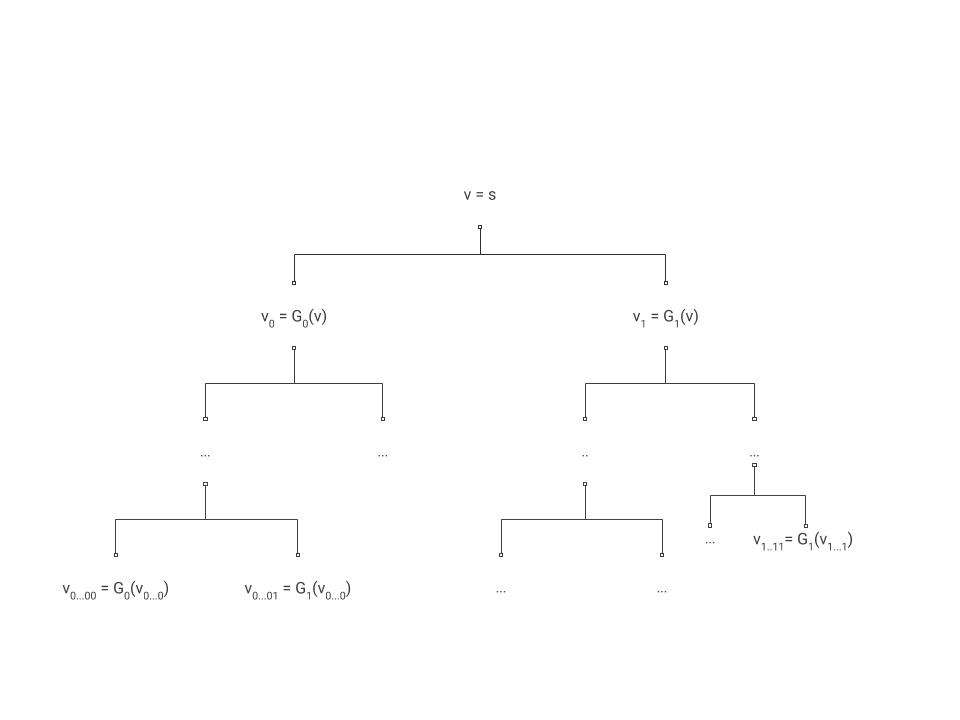
\includegraphics[width=\textwidth, height=0.25\paperheight, keepaspectratio]{../figure/PRF_from_PRG.jpg}
\caption{The construction of a pseudorandom function from a pseudorandom
generator can be illustrated by a depth \(n\) binary tree. The root is
labeled by the seed \(s\) and for every internal node \(v\) labeled by a
string \(x\in\{0,1\}^n\), we use that label \(x\) as a seed into the PRG
\(G\) to label \(v\)'s two children. In particular, the children of
\(v\) are labeled with \(G_0(x)\) and \(G_1(x)\) respectively. The
output of the function \(f_s\) on input \(i\) is the label of the
\(i^{th}\) leaf counting from left to right. Note that the numbering of
leaf \(i\) is related to the bitstring representation of \(i\) and the
path leaf \(i\) in the following way: we traverse to leaf \(i\) from the
root by reading off the \(n\) bits of \(i\) left to right and descend
into the left child of the current node for every 0 we encounter and
traverse right for every 1.}
\label{PRFfromPRGfig}
\end{figure}

\begin{proof} \label[proof]{5-We-describe-the-proof-}

We describe the proof, see also
\href{https://web.engr.oregonstate.edu/~rosulekm/crypto/chap6.pdf}{Chapter
6 of Rosulek} or Section 8.5 of Katz-Lindell (section 7.5 in 2nd
edition) for alternative expositions.

If the PRG Conjecture is true then in particular by the length extension
theorem there exists a PRG \(G:\{0,1\}^n\rightarrow\{0,1\}^{2n}\) that
maps \(n\) bits into \(2n\) bits. Let's denote
\(G(s)=G_0(s)\circ G_1(s)\) where \(\circ\) denotes concatenation. That
is, \(G_0(s)\) denotes the first \(n\) bits and \(G_1(s)\) denotes the
last \(n\) bits of \(G(s)\).

For \(i\in\{0,1\}^n\), we define \(f_s(i)\) as
\begin{equation*}
G_{i_n}(G_{i_{n-1}}(\cdots G_{i_1}(s))).
\end{equation*}
This corresponds to \(n\) composed applications of \(G_{b}\) for
\(b \in \{0,1\}\). If the \(j^{th}\) bit of \(i\)'s binary string is 0
then the \(j^{th}\) application of the PRG is \(G_{0}\) otherwise it is
\(G_{1}\). This series of successive applications starts with the
initial seed \(s\).

This definition directly corresponds to the depiction in
\cref{PRFfromPRGfig}, where the successive applications of \(G_{b}\)
correspond to the recursive labeling procedure.

By the definition above we can see that to evaluate \(f_s(i)\) we need
to evaluate the pseudorandom generator \(n\) times on inputs of length
\(n\), and so if the pseudorandom generator is efficiently computable
then so is the pseudorandom function. Thus, ``all'' that's left is to
prove that the construction is secure and this is the heart of this
proof.

I've mentioned before that the first step of writing a proof is
convincing yourself that the statement is true, but there is actually an
often more important zeroth step which is understanding what the
statement actually \emph{means}. In this case what we need to prove is
the following:

We need to show that the security of the PRG \(G\) implies the security
of the PRF ensemble \(\{ f_s \}\). Via the contrapositive, this means
that we assume that there is an adversary \(A\) that can distinguish in
time \(T\) a black box for \(f_s(\cdot)\) from a black-box for a random
function with advantage \(\epsilon\). We need to use \(A\) come up with
an adversary \(D\) that can distinguish in time \(poly(T)\) an input of
the form \(G(s)\) (where \(s\) is random in \(\{0,1\}^n\)) from an input
of the form \(y\) where \(y\) is random in \(\{0,1\}^{2n}\) with bias at
least \(\epsilon/poly(T)\).

\begin{marginfigure}
\centering
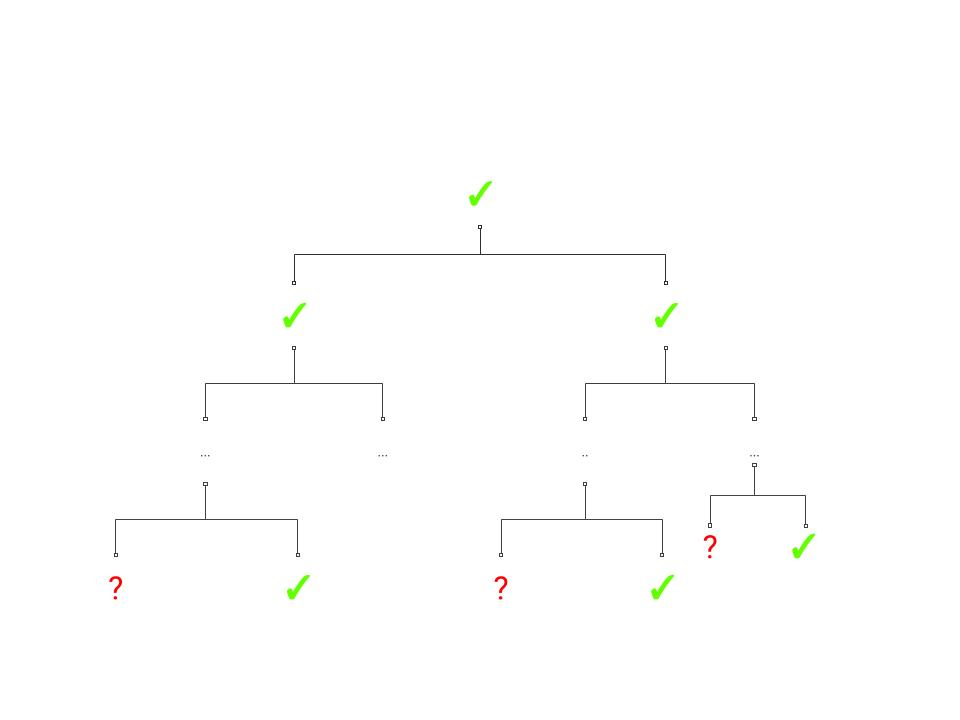
\includegraphics[width=\linewidth, height=1.5in, keepaspectratio]{../figure/Lazy_PRF_from_PRG.jpg}
\caption{In the ``lazy evaluation'' implementation of the black box to
the adversary, we label every node in the tree only when we need it.
Subsequent traversals do not reevaluate the PRG, leading to reuse of the
intermediate seeds. Thus for example, two sibling leaves will correspond
to a single call to \(G(x)\), where \(x\) is their parent's label, but
with the left child receiving the first \(n\) bits and the right child
receiving the second \(n\) bits of \(G(x)\). In this figure check marks
correspond to nodes that have been labeled and question marks to nodes
that are still unlabeled.}
\label{lazyevalprffig}
\end{marginfigure}

Assume that \(A\) as above is a \(T\)-time adversary that wins in the
``PRF game'' with advantage \(\epsilon\). Let us consider the ``lazy
evaluation'' implementation of the black box for \(A\) illustrated in
\cref{lazyevalprffig}. That is, at every point in time there are nodes
in the full binary tree that are labeled and nodes which we haven't yet
labeled. When \(A\) makes a query \(i\), this query corresponds to the
path \(i_1\ldots i_n\) in the tree. We look at the lowest (furthest away
from the root) node \(v\) on this path which has been labeled by some
value \(y\), and then we continue labelling the path from \(v\)
downwards until we reach \(i\). In other words, we label the two
children of \(v\) by \(G_0(y)\) and \(G_1(y)\), and then if the path
\(i\) involves the first child then we label its children by
\(G_0(G_0(y))\) and \(G_1(G_0(y))\), and so on and so forth (see
\cref{oracleevaltreefig}). Note that because \(G_{0}(y)\) and
\(G_{1}(y)\) correspond to a single call to \(G\), regardless of whether
the traversals continues left or right (i.e.~whether the current level
corresponds to a value 0 or 1 in \(i\)) we label both children at the
same time.

\begin{figure}
\centering
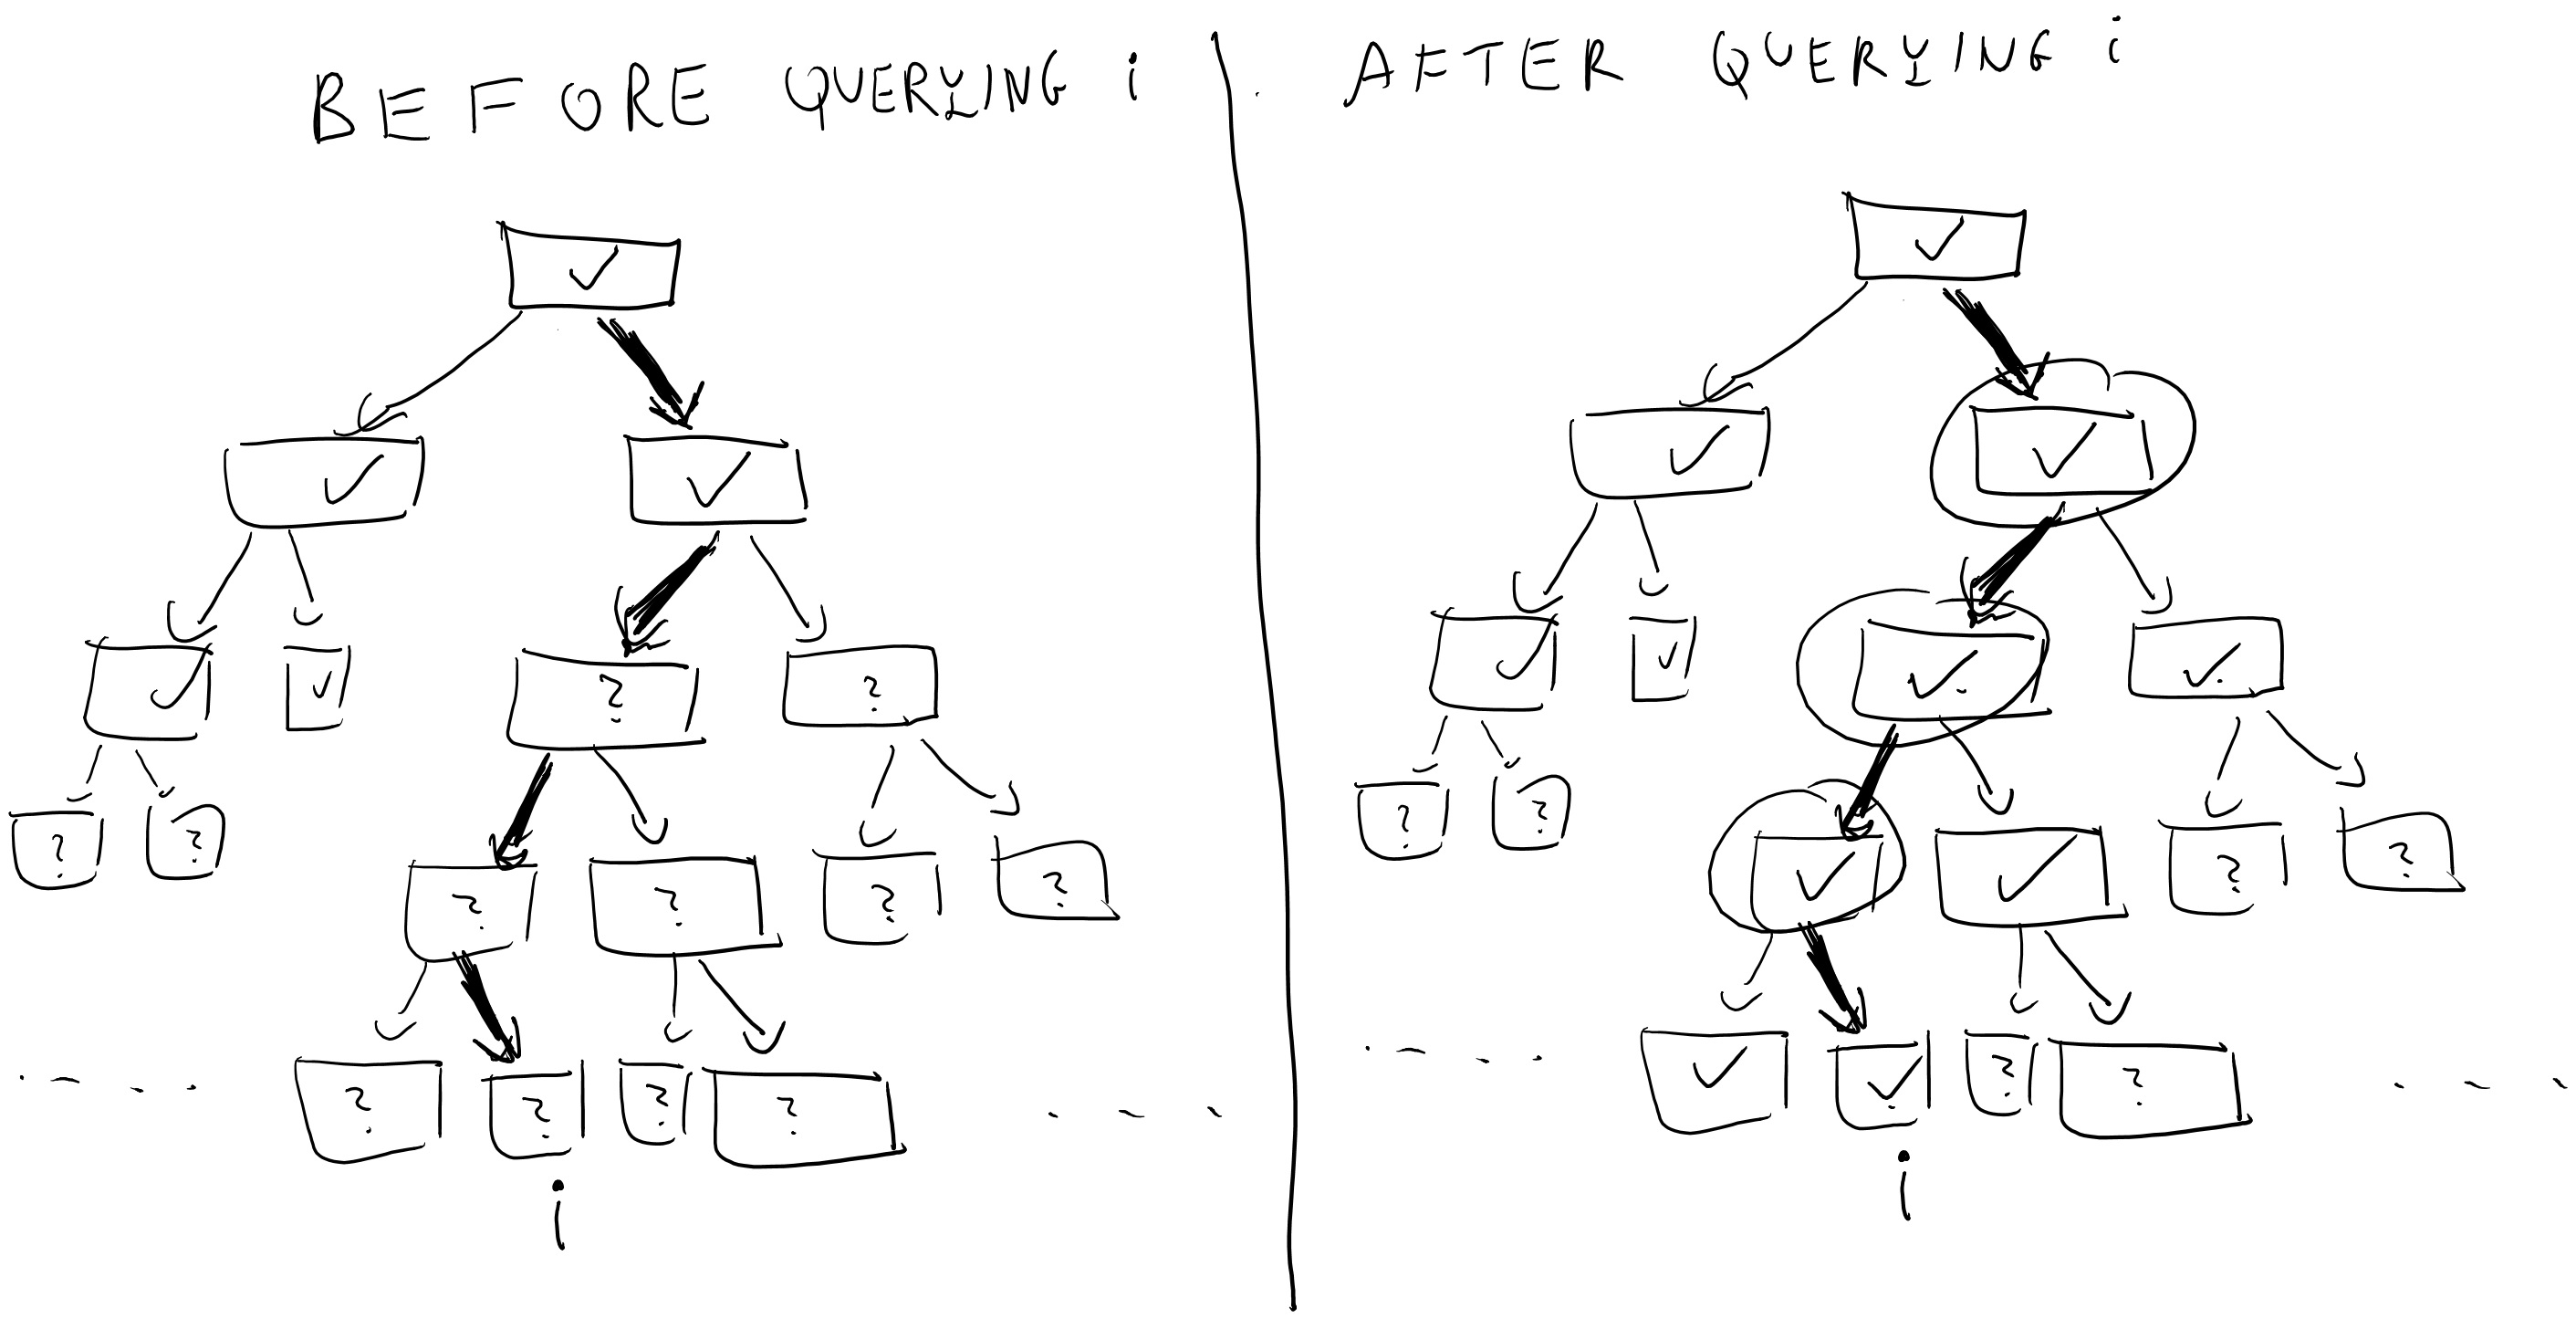
\includegraphics[width=\textwidth, height=0.25\paperheight, keepaspectratio]{../figure/prf-oracle-step.jpg}
\caption{When the adversary queries \(i\), the oracle takes the path
from \(i\) to the root and computes the generator on the minimum number
of internal nodes that is needed to obtain the label of the \(i^{th}\)
leaf.}
\label{oracleevaltreefig}
\end{figure}

A moment's thought shows that this is just another (arguably cumbersome)
way to describe the oracle that simply computes the map
\(i\mapsto f_s(i)\). And so the experiment of running \(A\) with this
oracle produces precisely the same result as running \(A\) with access
to \(f_s(\cdot)\). Note that since \(A\) has running time at most \(T\),
the number of times our oracle will need to label an internal node is at
most \(T' \leq 2nT\) (since we label at most \(2n\) nodes for every
query \(i\)).

We now define the following \(T'\) hybrids: in the \(j^{th}\) hybrid, we
run this experiment but in the first \(j\) times the oracle needs to
label internal nodes then it uses independent random labels. That is,
for the first \(j\) times we label a node \(v\), instead of letting the
label of \(v\) be \(G_b(u)\) (where \(u\) is the parent of \(v\), and
\(b\in \{0,1\}\) corresponds to whether \(v\) is the left or right child
of \(u\)), we label \(v\) by a random string in \(\{0,1\}^n\).

\begin{figure}
\centering
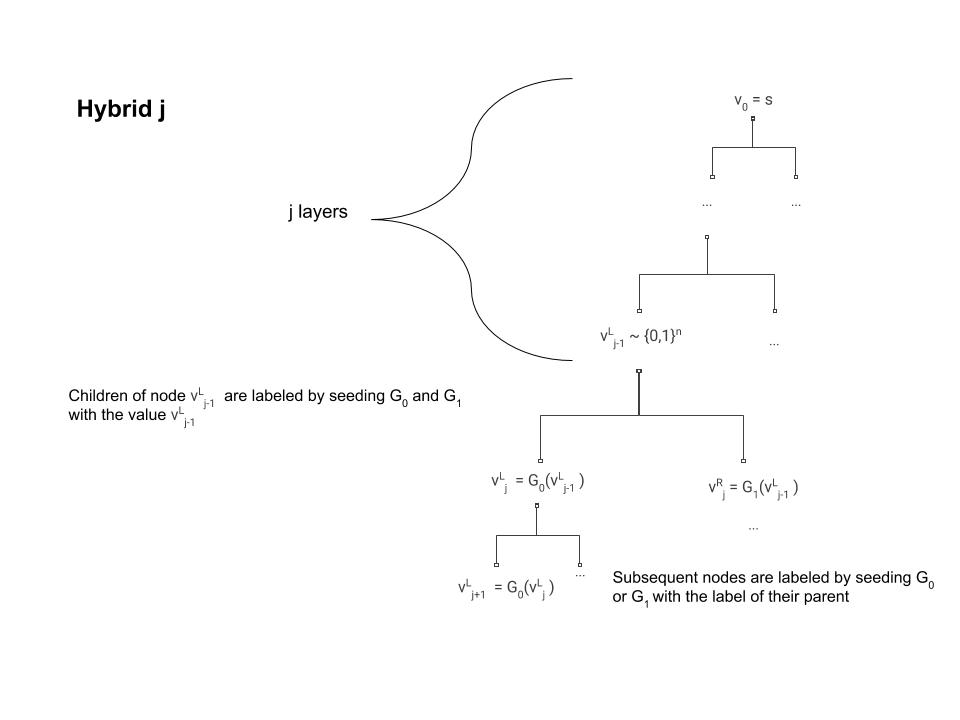
\includegraphics[width=\textwidth, height=0.25\paperheight, keepaspectratio]{../figure/hybrid_j_thm_5-1.jpg}
\caption{In the \(j^{th}\) hybrid the first \(j\) internal labels are
drawn uniformly at random from \(U_{n}\). All subsequent children's
labels are produced in the usual way by seeding \(G\) with the label
\(z\) of the parent and assigning the first \(n\) bits (\(G_{0}(z)\)) to
the left child and the last \(n\) bits (\(G_{1}(z)\)) to the right
child. For example, for some node \(v^{L}_{j-1}\) at the \(j^{th}\)
level, we generate pseudorandom string \(G(v^{L}_{j-1})\) and label the
left child \(v^{L}_{j} = G_{0}(v^{L}_{j-1})\) and the right child
\(v^{R}_{j} = G_{1}(v^{L}_{j-1})\). Note that the labeling scheme for
this diagram is different from that in the previous figures. This is
simply for ease of exposition, we could still index our nodes via the
path reaching them from the root.}
\label{hybridj}
\end{figure}

\begin{figure}
\centering
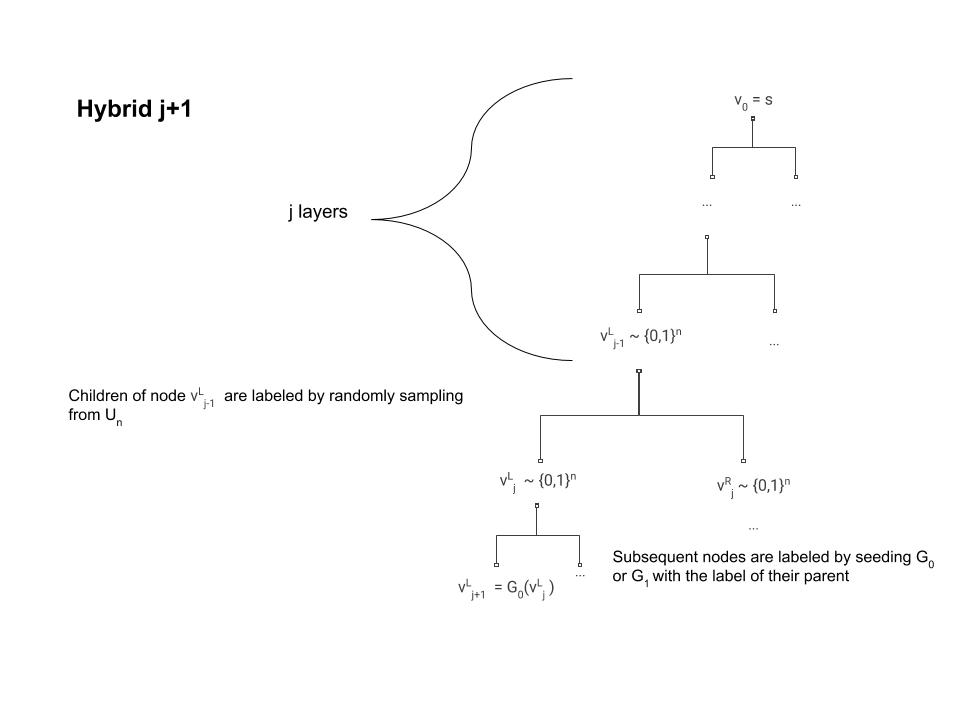
\includegraphics[width=\textwidth, height=0.25\paperheight, keepaspectratio]{../figure/hybrid_j1_thm_5-1.jpg}
\caption{The \(j+1^{st}\) hybrid differs from the \(j^{th}\) in that the
process of assigning random labels continues until the \(j+1^{st}\) step
as opposed to the \(j^{th}\). The hybrids are otherwise completely
identically constructed.}
\label{hybridj1}
\end{figure}

Note that the \(0^{th}\) hybrid corresponds to the case where the oracle
implements the function \(i\mapsto f_s(i)\), while in the \(T'^{th}\)
hybrid all labels are random and hence implements a random function. By
the hybrid argument, if \(A\) can distinguish between the \(0^{th}\)
hybrid and the \(T'^{th}\) hybrid with bias \(\epsilon\) then there must
exists some \(j\) such that it distinguishes between the \(j^{th}\)
hybrid (pictured in \cref{hybridj}) and the \(j+1^{st}\) hybrid
(pictured in \cref{hybridj1}) with bias at least \(\epsilon/T'\). We
will use this \(j\) and \(A\) to break the pseudorandom generator.

\begin{figure}
\centering
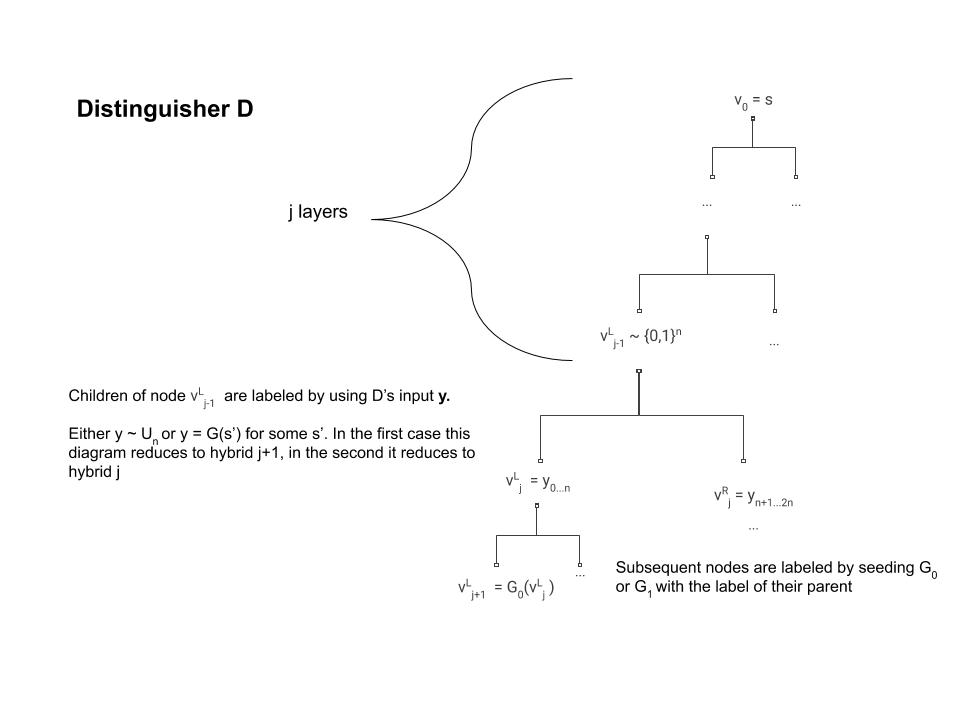
\includegraphics[width=\textwidth, height=0.25\paperheight, keepaspectratio]{../figure/distinguisher_D_thm_5-1.jpg}
\caption{Distinguisher D is similar to hybrid \(j\), in that the nodes
in the first \(j\) layers are assigned completely random labels. When
evaluating along a particular path through \(v_{j-1}^{L}\), rather than
labeling the two children by applying \(G\) to its label, it simply
splits the input \(y\) into two strings \(y_{0...n}\),\(y_{n+1...2n}\).
If \(y\) is truly random, \(D\) is identical to hybrid \(j+1\). If
\(y=G(s)\) for some random seed \(s\), then \(D\) simulates hybrid
\(j\).}
\label{distinguisherd}
\end{figure}

We can now describe our distinguisher \(D\) (see \cref{distinguisherd})
for the pseudorandom generator. On input a string \(y\in\{0,1\}^{2n}\)
\(D\) will run \(A\) and the \(j^{th}\) oracle inside its belly with one
difference- when the time comes to label the \(j^{th}\) node, instead of
doing this by applying the pseudorandom generator to the label of its
parent \(v\) (which is what should happen in the \(j^{th}\) oracle) it
uses its input \(y\) to label the two children of \(v\).

Now, if \(y\) was completely random then we get exactly the distribution
of the \(j+1^{st}\) oracle, and hence in this case \(D\) simulates
internally the \(j+1^{st}\) hybrid. However, if \(y=G(s)\) for some
randomly sampled \(s\in\{0,1\}^n\), though it may not be obvious at
first, we actually get the distribution of the \(j^{th}\) oracle.

The equivalence between hybrid \(j\) and distinguisher \(D\) under the
condition that \(y=G(s)\) is non obvious, because in hybrid \(j\), the
label for the children of \(v_{j-1}^{L}\) was supposed to be the result
of applying the pseudorandom generator to the label of \(v_{j-1}^{L}\)
and not to some other random string (see \cref{distinguisherd}).
However, because \(v\) was labeled \emph{before} the \(j^{th}\) step
then we know that it was actually labeled by a random string. Moreover,
since we use lazy evaluation we know that step \(j\) is the \emph{first}
time where we actually use the value of the label of \(v\). Hence, if at
this point we \emph{resampled} this label and used a completely
independent random string \(s\) then the distribution of \(v_{j-1}^{L}\)
and \(s\) would be \emph{identical}.

The key observations here are:

\begin{enumerate}
\def\labelenumi{\arabic{enumi}.}
\item
  The output of \(A\) does not directly depend on the internal labels,
  but only on the labels of the leaves (since those are the only values
  returned by the oracle).
\item
  The label for an internal vertex \(v\) is only used once, and that is
  for generating the labels for its children.
\end{enumerate}

Hence the distribution of \(y=G(s)\), for \(s\) drawn from \(U_n\), is
identical to the distribution, \(G(v_{j-1}^{L})\), of the \(j^{th}\)
hybrid, and thus if \(A\) had advantage \(\epsilon\) in breaking the PRF
\(\{ f_s \}\) then \(D\) will have advantage \(\epsilon/T'\) in breaking
the PRG \(G\) thus obtaining a contradiction.

\end{proof}

\hypertarget{prfpracticerem}{}
\begin{remark}[PRF's in practice] \label[remark]{prfpracticerem}

While this construction reassures us that we can rely on the existence
of pseudorandom functions even on days where we remember to take our
meds, this is not the construction people use when they need a PRF in
practice because it is still somewhat inefficient, making \(n\) calls to
the underlying pseudorandom generators. There are constructions (e.g.,
HMAC) based on hash functions that require stronger assumptions but can
use as few as two calls to the underlying function. We will cover these
constructions when we talk about hash functions and the random oracle
model. One can also obtain practical constructions of PRFs from
\emph{block ciphers}, which we'll see later in this lecture.

\end{remark}

\section{Securely encrypting many messages - chosen plaintext
security}\label{5-Securely-encrypting-ma}

Let's get back to our favorite task of \emph{encryption}. We seemed to
have nailed down the definition of secure encryption, or did we?

\begin{pause} \label[pause]{5-Try-to-think-what-kind}

Try to think what kind of security guarantees are \emph{not} provided by
the notion of computational secrecy we saw in \cref{compsecdef}

\end{pause}

\cref{compsecdef} talks about encrypting a \emph{single} message, but
this is not how we use encryption in the real world. Typically, Alice
and Bob (or Amazon and Boaz) setup a shared key and then engage in many
back and forth messages between one another. At first, we might think
that this issue of a single long message vs.~many short ones is merely a
technicality. After all, if Alice wants to send a sequence of messages
\((m_1,m_2,\ldots,m_t)\) to Bob, she can simply treat them as a single
long message. Moreover, the way that \emph{stream ciphers} work, Alice
can compute the encryption for the first few bits of the message she
decides what will be the next bits and so she can send the encryption of
\(m_1\) to Bob and later the encryption of \(m_2\). There is some truth
to this sentiment, but there are issues with using stream ciphers for
multiple messages. For Alice and Bob to encrypt messages in this way,
they must maintain a \emph{synchronized shared state}. If the message
\(m_1\) was dropped by the network, then Bob would not be able to
decrypt correctly the encryption of \(m_2\).

There is another way in which treating many messages as a single tuple
is unsatisfactory. In real life, Eve might be able to have some impact
on \emph{what} messages Alice encrypts. For example, the Katz-Lindell
book describes several instances in World War II where Allied forces
made particular military maneuver for the sole purpose of causing the
Axis forces to send encryptions of messages of the Allies' choosing. To
consider a more modern example, today Google uses encryption for all of
its search traffic including (for the most part) the \emph{ads} that are
displayed on the page. But this means that an attacker, by paying
Google, can cause it to encrypt arbitrary text of their choosing. This
kind of attack, where Eve \emph{chooses} the message she wants to be
encrypted is called a \emph{chosen plaintext attack}. You might think
that we are already covering this with our current definition that
requires security \emph{for every} pair of messages and so in particular
this pair could be chosen by Eve. However, in the case of multiple
messages, we would want to allow Eve to be able to choose \(m_2\)
\emph{after} she saw the encryption of \(m_1\).

All that leads us to the following definition, which is a strengthening
of our definition of computational security:

\hypertarget{cpasecuredef}{}
\begin{definition}[Chosen Plaintext Attack (CPA) secure encryption] \label[definition]{cpasecuredef}

An encryption scheme \((E,D)\) is \emph{secure against chosen plaintext
attack (CPA secure)} if for every polynomial time \(Eve\), Eve wins with
probability at most \(1/2+negl(n)\) in the game defined below:

\begin{enumerate}
\def\labelenumi{\arabic{enumi}.}
\tightlist
\item
  The key \(k\) is chosen at random in \(\{0,1\}^n\) and fixed.
\item
  Eve gets the length of the key \(1^n\) as input.\footnote{Giving Eve
    the key as a sequence of \(n\) \(1'\)s as opposed to in binary
    representation is a common notational convention in cryptography. It
    makes no difference except that it makes the input length for Eve of
    length \(n\), which makes sense since we want to allow Eve to run in
    \(poly(n)\) time.}
\item
  Eve interacts with \(E\) for \(t=poly(n)\) rounds as follows: in the
  \(i^{th}\) round, Eve chooses a message \(m_i\) and obtains
  \(c_i= E_k(m_i)\).
\item
  Then Eve chooses two messages \(m_0,m_1\), and gets \(c^* = E_k(m_b)\)
  for \(b\leftarrow_R\{0,1\}\).
\item
  Eve continues to interact with \(E\) for another \(poly(n)\) rounds,
  as in Step 3.
\item
  Eve \emph{wins} if she outputs \(b\).
\end{enumerate}

\end{definition}

\begin{marginfigure}
\centering
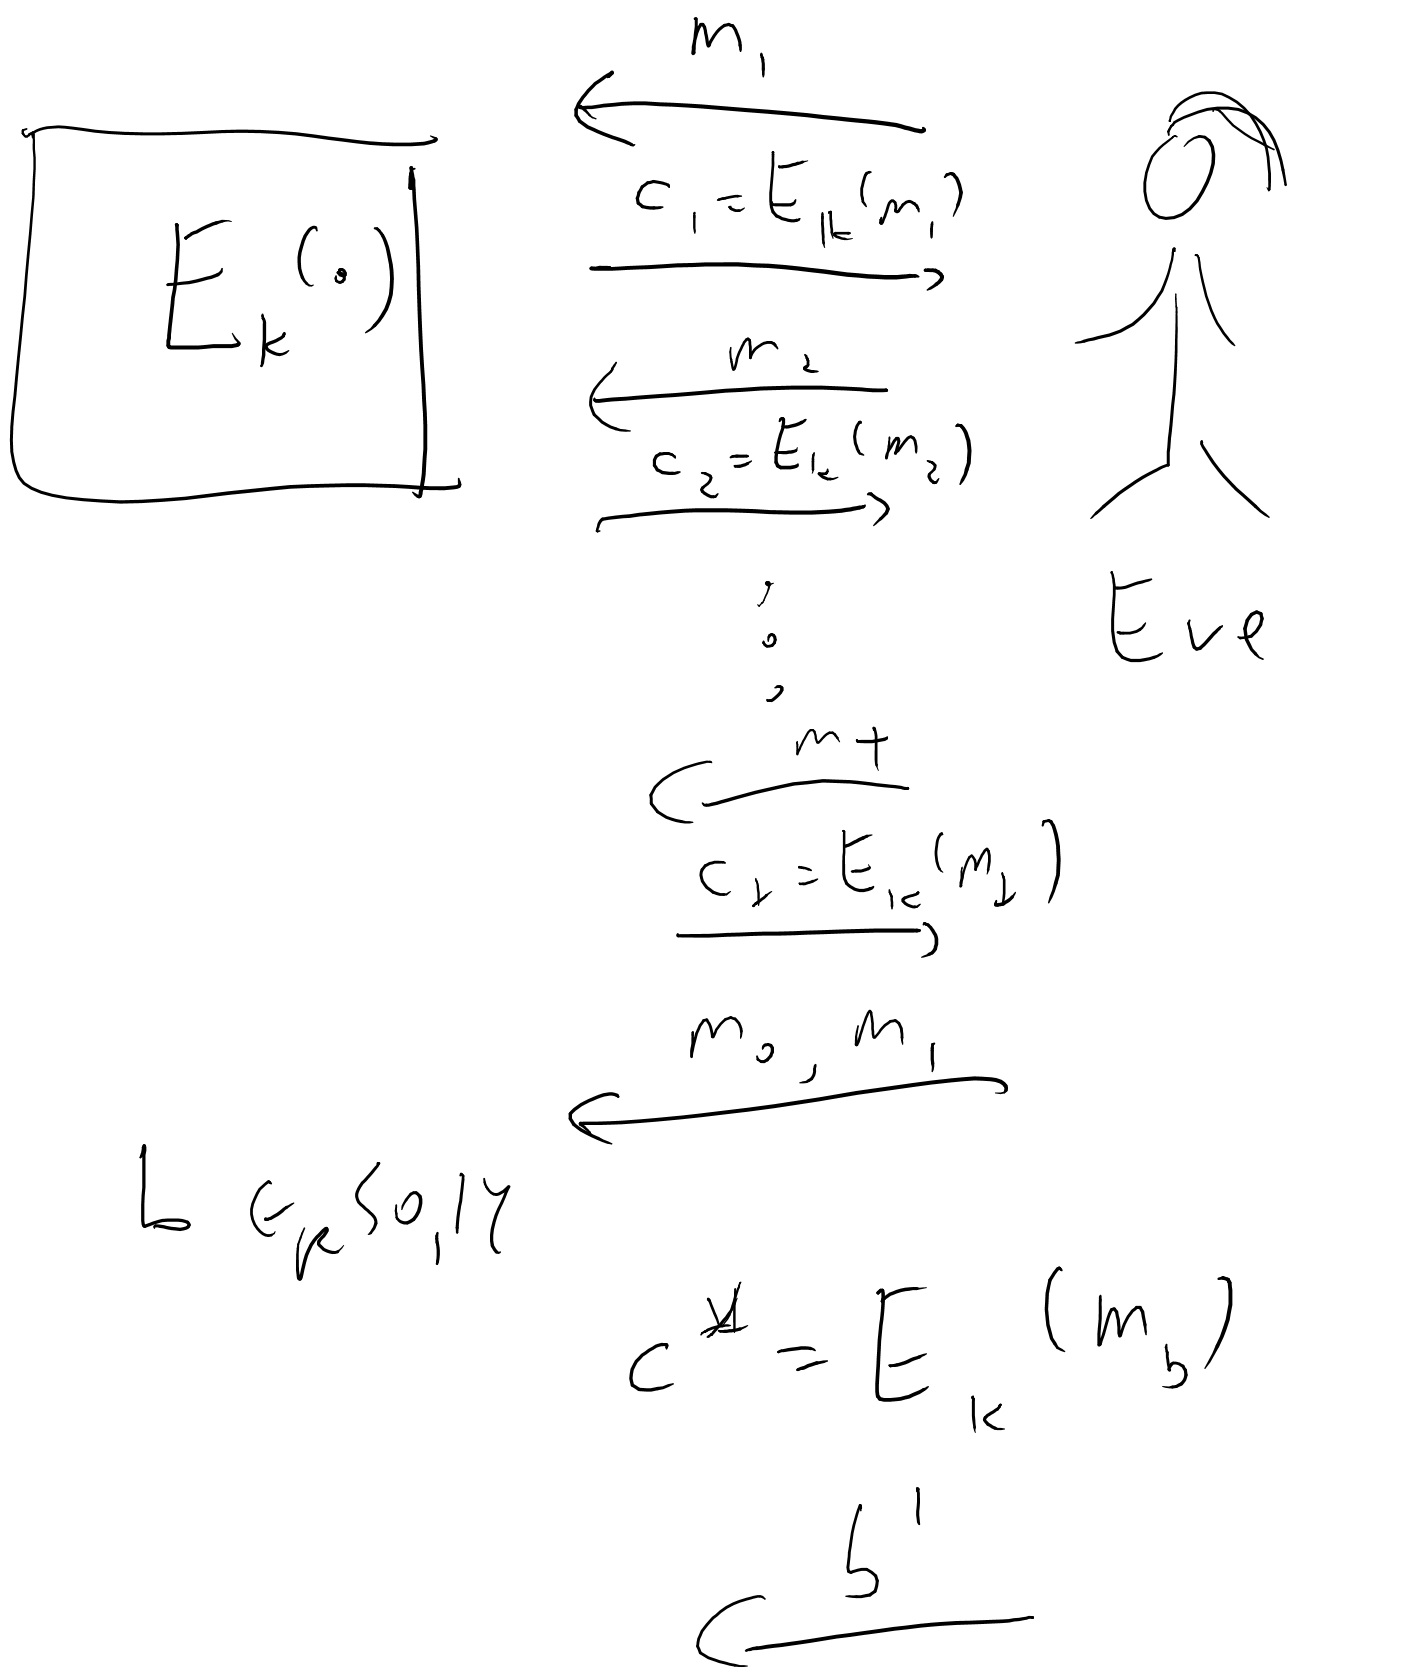
\includegraphics[width=\linewidth, height=1.5in, keepaspectratio]{../figure/cpa-game.jpg}
\caption{In the CPA game, Eve interacts with the encryption oracle and
at the end chooses \(m_0,m_1\), gets an encryption \(c^*=E_k(m_b)\) and
outputs \(b'\). She \emph{wins} if \(b'=b\)}
\label{cpasecgamefig}
\end{marginfigure}

\cref{cpasecuredef} is illustrated in \cref{cpasecgamefig}. Our previous
notion of computational secrecy (i.e., \cref{compsecdef}) corresponds to
the case that we skip Steps 3 and 5 above. Since Steps 3 and 5 only give
the adversary more power (and hence is only more likely to win), CPA
security (\cref{cpasecuredef}) is \emph{stronger} than computational
secrecy (\cref{compsecdef}), in the sense that every CPA secure
encryption \((E,D)\) is also computationally secure. It turns out that
CPA security is \emph{strictly stronger}, in the sense that without
modification, our stream ciphers cannot be CPA secure. In fact, we have
a stronger, and intially somewhat surprising theorem:

\hypertarget{CPAsecrandomthm}{}
\begin{theorem}[CPA security requires randomization] \label[theorem]{CPAsecrandomthm}

There is no CPA secure \((E,D)\) where \(E\) is \emph{deterministic}.

\end{theorem}

\begin{proof} \label[proof]{5-The-proof-is-very-simp}

The proof is very simple: Eve will only use a single round of
interacting with \(E\) where she will ask for the encryption \(c_1\) of
\(0^\ell\). In the second round, Eve will choose \(m_0=0^{\ell}\) and
\(m_1=1^{\ell}\), and get \(c^*=E_k(m_b)\) she will then output \(0\) if
and only if \(c^*=c_1\).

\end{proof}

\begin{marginfigure}
\centering
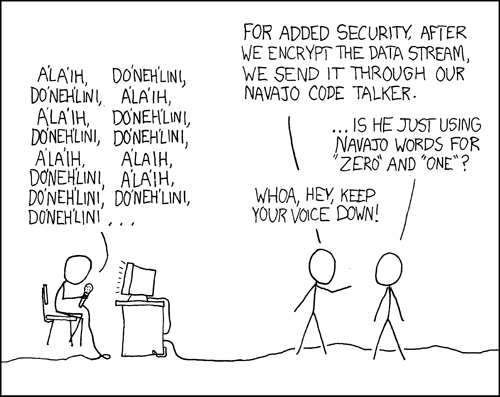
\includegraphics[width=\linewidth, height=1.5in, keepaspectratio]{../figure/code_talkers.png}
\caption{Insecurity of deterministic encryption}
\label{xkcdnavajotwofig}
\end{marginfigure}

This proof is so simple that you might think it shows a problem with the
definition, but it is actually a real problem with security. If you
encrypt many messages and some of them repeat themselves, it is possible
to get significant information by seeing the repetition pattern (cue the
XKCD cartoon again, see \cref{xkcdnavajotwofig}). To avoid this issue we
need to use a \emph{randomized} (or \emph{probabilistic}) encryption,
such that if we encrypt the same message twice we \emph{won't} see two
copies of the same ciphertext.\footnote{If the messages are guaranteed
  to have \emph{high entropy} which roughly means that the probability
  that a message repeats itself is negligible, then it is possible to
  have a secure deterministic private-key encryption, and this is
  sometimes used in practice. (Though often some sort of randomization
  or padding is added to ensure this property, hence in effect creating
  a randomized encryption.) Deterministic encryptions can sometimes be
  useful for applications such as efficient queries on encrypted
  databases. See \href{https://goo.gl/GWJLFd}{this lecture} in Dan
  Boneh's coursera course.} But how do we do that? Here pseudorandom
functions come to the rescue:

\hypertarget{cpafromprfthm}{}
\begin{theorem}[CPA security from PRFs] \label[theorem]{cpafromprfthm}

Suppose that \(\{ f_s \}\) is a PRF collection where
\(f_s:\{0,1\}^n\rightarrow\{0,1\}^\ell\), then the following is a CPA
secure encryption scheme: \(E_s(m)=(r,f_s(r)\oplus m)\) where
\(r \leftarrow_R \{0,1\}^n\), and \(D_s(r,z)=f_s(r)\oplus z\).

\end{theorem}

\begin{proof} \label[proof]{5-I-leave-to-you-to-veri}

I leave to you to verify that \(D_s(E_s(m))=m\). We need to show the CPA
security property. As is usual in PRF-based constructions, we first show
that this scheme will be secure if \(f_s\) was an actually random
function, and then use that to derive security.

Consider the game above when played with a completely random function
and let \(r_i\) be the random string chosen by \(E\) in the \(i^{th}\)
round and \(r^*\) the string chosen in the last round. We start with the
following simple but crucial claim:

\textbf{Claim:} The probability that \(r^*=r_i\) for some \(i\) is at
most \(T/2^n\).

\textbf{Proof of claim:} For any particular \(i\), since \(r^*\) is
chosen independently of \(r_i\), the probability that \(r^*=r_i\) is
\(2^{-n}\). Hence the claim follows from the union bound. QED

Given this claim we know that with probability \(1-T/2^n\) (which is
\(1-negl(n)\)), the string \(r^*\) is distinct from any string that was
chosen before. This means that by the lazy evaluation principle, if
\(f_s(\cdot)\) is a completely random function then the value
\(f_s(r^*)\) can be thought of as being chosen at random in the final
round independently of anything that happened before. But then
\(f_s(r^*)\oplus m_b\) amounts to simply using the one-time pad to
encrypt \(m_b\). That is, the distributions \(f_s(r^*)\oplus m_0\) and
\(f_s(r^*)\oplus m_1\) (where we think of \(r^*,m_0,m_1\) as fixed and
the randomness comes from the choice of the random function
\(f_s(\cdot)\)) are both equal to the uniform distribution \(U_n\) over
\(\{0,1\}^n\) and hence Eve gets absolutely no information about \(b\).

This shows that if \(f_s(\cdot)\) was a random function then Eve would
win the game with probability at most \(1/2\). Now if we have some
efficient Eve that wins the game with probability at least
\(1/2+\epsilon\) then we can build an adversary \(A\) for the PRF that
will run this entire game with black box access to \(f_s(\cdot)\) and
will output \(1\) if and only if Eve wins. By the argument above, there
would be a difference of at least \(\epsilon\) in the probability it
outputs \(1\) when \(f_s(\cdot)\) is random vs when it is pseudorandom,
hence contradicting the security property of the PRF.

\end{proof}

\section{Pseudorandom permutations / block
ciphers}\label{5-Pseudorandom-permutati}

Now that we have pseudorandom functions, we might get greedy and want
such functions with even more magical properties. This is where the
notion of \emph{pseudorandom permutations} comes in.

::: \{.definition title=``Pseudorandom permutations'' \#PRPdef\} Let
\(\ell:\N \rightarrow \N\) be some function that is polynomially bounded
(i.e., there are some \(0<c<C\) such that \(n^c < \ell(n) < n^C\) for
every \(n\)). A collection of functions \(\{ f_s \}\) where
\(f_s:\{0,1\}^{\ell} \rightarrow\{0,1\}^{\ell}\) for \(\ell=\ell(|s|)\)
is called a \emph{pseudorandom permutation (PRP) collection} if:

\begin{enumerate}
\def\labelenumi{\arabic{enumi}.}
\tightlist
\item
  It is a pseudorandom function collection (i.e., the map
  \(s,x \mapsto f_s(x)\) is efficiently computable and there is no
  efficient distinguisher between \(f_s(\cdot)\) with a random \(s\) and
  a random function).\\
\item
  Every function \(f_s\) is a permutation of \(\{0,1\}^\ell\) (i.e., a
  one to one and onto map).\\
\item
  There is an efficient algorithm that on input \(s,y\) returns
  \(f_s^{-1}(y)\). The parameter \(n\) is known as the \emph{key length}
  of the pseudorandom permutation collection and the parameter
  \(\ell=\ell(n)\) is known as the \emph{input length} or \emph{block
  length}. Often, \(\ell=n\) and so in most cases you can safely ignore
  this distinction.
\end{enumerate}

\begin{pause} \label[pause]{5-At-first-look-crefPRPd}

At first look \cref{PRPdef} might seem not to make sense, since on one
hand it requires the map \(x \mapsto f_s(x)\) to be a permutation, but
on the other hand it can be shown that with high probability a random
map \(H:\{0,1\}^\ell \rightarrow \{0,1\}^\ell\) will \emph{not} be a
permutation. How can then such a collection be pseudorandom? The key
insight is that while a random map might not be a permutation, it is not
possible to distinguish with a polynomial number of queries between a
black box that computes a random function and a black box that computes
a random permutation. Understanding why this is the case, and why this
means that \cref{PRPdef} is reasonable, is crucial to getting intuition
to this notion, and so I suggest you pause now and make sure you
understand these points.

\end{pause}

As usual with a new concept, we want to know whether it is possible to
achieve it and whether it is useful. The former is established by the
following theorem:

\hypertarget{PRPfromPRF}{}
\begin{theorem}[PRP's from PRFs] \label[theorem]{PRPfromPRF}

If the PRF conjecture holds (and hence by \cref{prfthm} also if the PRG
conjecture holds) then there exists a pseudorandom permutation
collection.

\end{theorem}

\begin{figure}
\centering
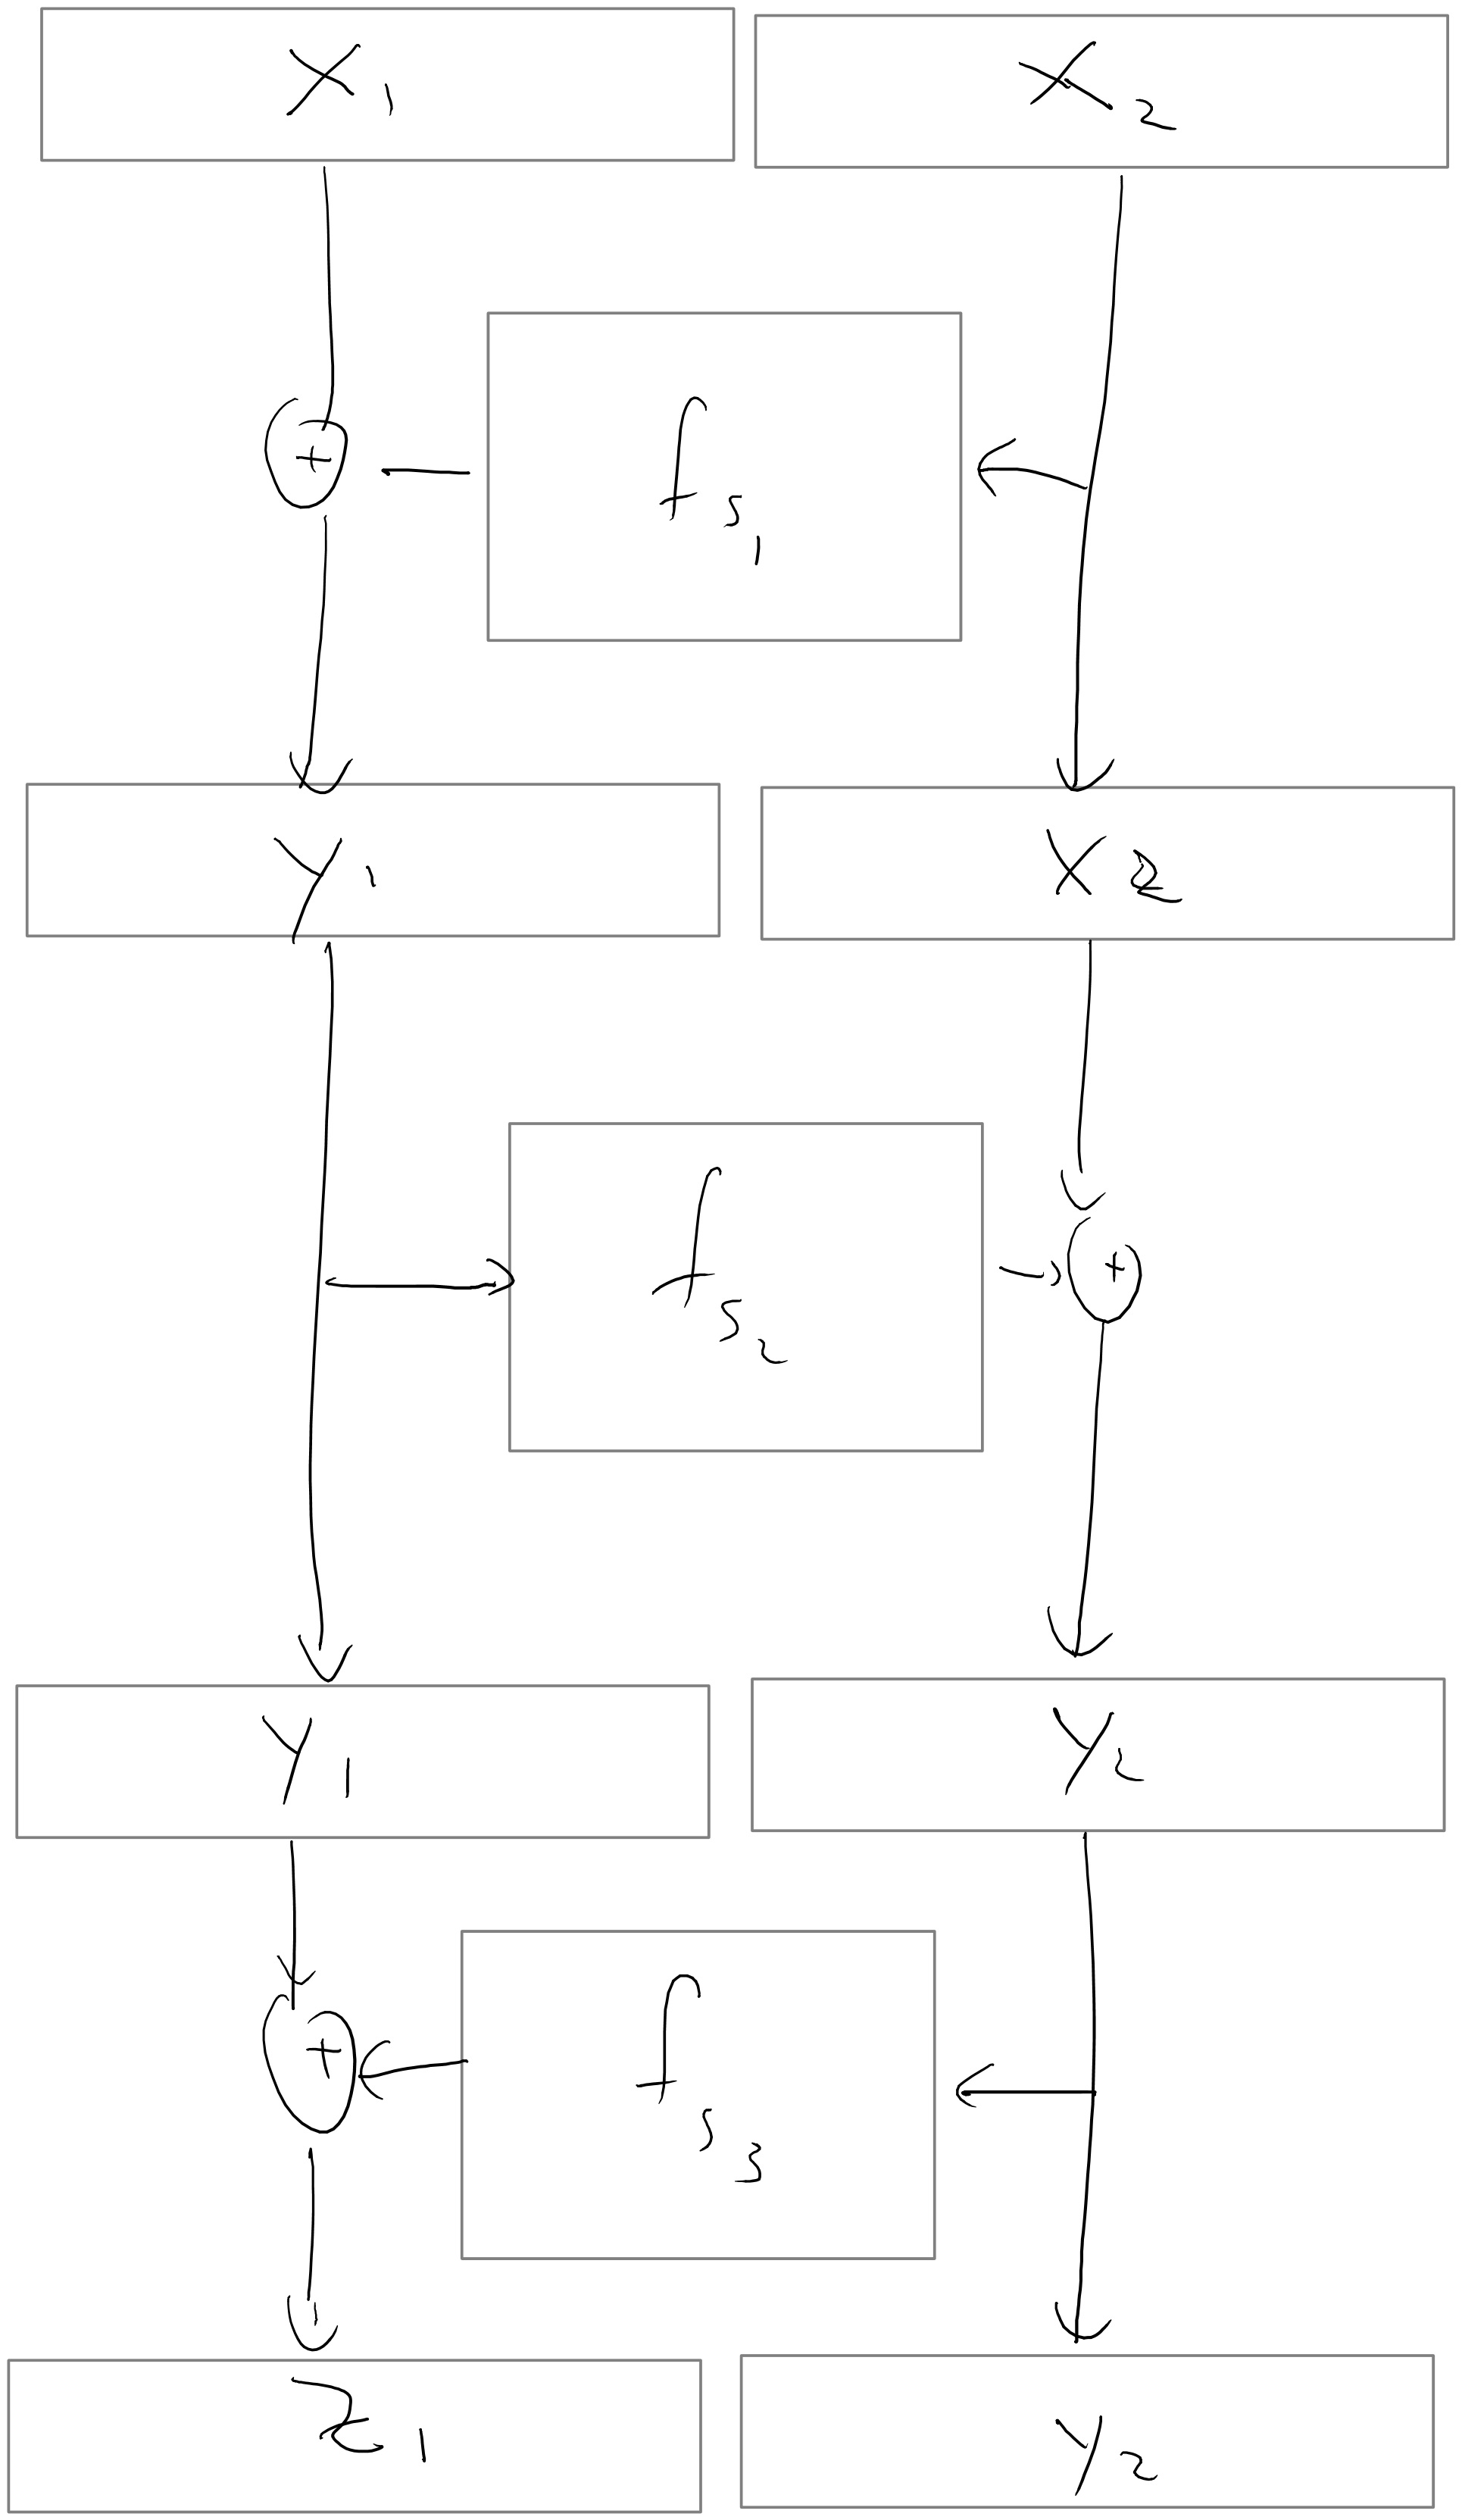
\includegraphics[width=\textwidth, height=0.25\paperheight, keepaspectratio]{../figure/feistel.jpg}
\caption{We build a PRP \(p\) on \(2n\) bits from three PRFs
\(f_{s_1},f_{s_2},f_{s_3}\) on \(n\) bits by letting
\(p_{s_1,s_2,s_3}(x_1,x_2)=(z_1,y_2)\) where
\(y_1 = x_1 \oplus f_{s_1}(x_2)\), \(y_2 = x_2 \oplus f_{s_2}(y_1)\) and
\(z_1 = f_{s_3}(y_2) \oplus y_1\).}
\label{feistelfig}
\end{figure}

\begin{proof} \label[proof]{5-creffeistelfig-illustr}

\cref{feistelfig} illustrates the construction of a pseudorandom
permutation from a pseudorandom function. The construction (known as the
Luby-Rackoff construction) uses several rounds of what is known as the
\href{https://en.wikipedia.org/wiki/Feistel_cipher}{Feistel
Transformation} that maps a function
\(f:\{0,1\}^n \rightarrow \{0,1\}^n\) into a permutation
\(g:\{0,1\}^{2n} \rightarrow \{0,1\}^{2n}\) using the map
\((x,y) \mapsto (x,f(x) \oplus y)\).

Specifically, given a PRF family \(\{f_s\}\) with \(n\)-bit keys,
inputs, and outputs, our candidate PRP family will be called
\(\{p_{s_1,s_2,s_3}\}\). Here,
\(p_{s_1,s_2, s_3}:\{0,1\}^{2n} \to \{0,1\}^{2n}\) is calculated on
input \((x_1, x_2) \in \{0,1\}^{2n}\) as follows (see
\cref{feistelfig}):

\begin{itemize}
\tightlist
\item
  First, map \((x_1, x_2) \mapsto (y_1, x_2)\), where
  \(y_1 = x_1 \oplus f_{s_1}(x_2)\).
\item
  Next, map \((y_1, x_2) \mapsto (y_1, y_2)\), where
  \(y_2 = x_2 \oplus f_{s_2}(y_1)\).
\item
  Next, map \((y_1, y_2) \mapsto (z_1, y_2)\), where
  \(z_1 = y_1 \oplus f_{s_3}(y_2)\).
\item
  Finally, output \(p_{s_1,s_2,s_3}(x_1,x_2) = (z_1, y_2)\).
\end{itemize}

Each of the first three steps above corresponds to a single round of the
Feistel transformation, which is easily seen to be both efficiently
computable \emph{and} efficiently invertible. In fact, we can
efficiently calculate \(p_{s_1,s_2,s_3}^{-1}(z_1, y_2)\) for an
arbitrary string \((z_1,y_2) \in \{0,1\}^{2n}\) by running the above
three rounds of Feistel transformations in reverse order.

Thus, the real challenge in proving \cref{PRPfromPRF} is not showing
that \(\{p_{s_1,s_2,s_3}\}\) is a valid permutation, but rather showing
that it is \emph{pseudorandom}. The details of remainder of this proof
are a bit technical, and can be safely skipped on a first reading.

Intuitively, the argument goes like this. Consider an oracle
\(\mathcal{O}\) for \(p_{s_1,s_2,s_3}\) that answers an adversary's
query \((x_1, x_2)\) by carrying out the three Feistel transformations
outlined above and outputting \((z_1, y_2)\). First, we'll show that
with high probability, \(\mathcal{O}\) will never encounter the same
intermediate string \(y_1\) twice, over the course of all queries
(unless the adversary makes a duplicate query). Since the string
\(y_1\), calculated in Step 1, determines the input on which \(f_{s_2}\)
is evaluated in Step 2, it follows that the strings \(y_2\) calculated
in Step 2 will appear to be chosen independently and at random. In
particular, \emph{they too} will be pairwise distinct with high
probability. Since the string \(y_2\) is in turn passed as input to
\(f_{s_3}\) in Step 3, it follows that the strings \(z_1\) encountered
over the course of all queries will also appear to be chosen
independently and at random. Ultimately, this means that the oracle's
outputs \((z_1, y_2)\) will look like freshly independent, random
strings.

To make this reasoning precise, notice first that it suffices to
establish the security of a \emph{variant} of \(p_{s_1,s_2,s_3}\) in
which the pseudorandom functions \(f_{s_1}\), \(f_{s_2}\), and
\(f_{s_3}\) used in the construction are replaced by truly random
functions \(h_1,h_2,h_3 : \{0,1\}^n \to \{0,1\}^n\). Call this variant
\(p_{h_1,h_2,h_3}\). Indeed, the assumption that \(\{f_s\}\) is a PRF
collection tells us that making this change has only a negligible effect
on the output of an adversary with oracle access to \(p\). With this in
mind, our job is to show that for every efficient adversary \(A\), the
difference
\(|\Pr[A^{p_{h_1,h_2,h_3}(\cdot)}(1^n)=1] - \Pr[A^{H(\cdot)}(1^n)=1]|\)
is negligible. In this expression, the first probability is taken over
the choice of the random functions
\(h_1,h_2,h_3 :\{0,1\}^n \to \{0,1\}^n\) used in the Feistel
transformation, and the second probability is taken over the random
function \(H : \{0,1\}^{2n} \to \{0,1\}^{2n}\). To simplify matters,
suppose without loss of generality that \(A\) always makes \(q(n)\)
\emph{distinct} queries to its oracle, denoted
\((x_1^{(1)}, x_2^{(1)}), \ldots, (x_1^{(q(n))}, x_2^{(q(n))})\) in
order. Similarly, let \(y_1^{(i)}, y_2^{(i)}, z_1^{(i)}\) denote the
intermediate strings calculated in the three rounds of the Feistel
transformation. Here, \(q\) is a polynomial in \(n\).

Consider the case in which the adversary \(A\) is interacting with the
oracle for \(p_{h_1,h_2,h_3}\), as opposed to the random oracle. Let us
say that a \emph{collision occurs at \(y_1\)} if for some
\(1 \le i < j \le q(n)\), the string \(y_1^{(i)}\) computed while
answering \(A\)'s \(i\)th query coincides with the string \(y_1^{(j)}\)
computed while answering \(A\)'s \(j\)th query. We claim the probability
that a collision occurs at \(y_1\) is negligibly small. Indeed, if a
collision occurs at \(y_1\), then \(y_1^{(i)} = y_1^{(j)}\) for some
\(i \neq j\). By the construction of \(p_{h_1,h_2,h_3}\), this means
that
\(x_1^{(i)} \oplus h_1(x_2^{(i)}) = x_1^{(j)} \oplus h_1(x_2^{(j)})\).
In particular, it cannot be the case that \(x_1^{(i)} \neq x_1^{(j)}\)
and \(x_2^{(i)} = x_2^{(j)}\). Since we assumed that \(A\) makes
distinct queries to its oracle, it follows that
\(x_2^{(i)} \neq x_2^{(j)}\) and hence that \(h_1(x_2^{(i)})\) and
\(h_1(x_2^{(j)})\) are uniform and independent. In other words,
\(\Pr[y_1^{(i)} = y_1^{(j)}] = \Pr[x_1^{(i)} \oplus f_1(x_2^{(i)}) = x_1^{(j)} \oplus f_1(x_2^{(j)})] = 2^{-n}\).
Taking a union bound over all choices of \(i\) and \(j\), we see that
the probability of a collision at \(y_1\) is at most \(q(n)^2/2^n\),
which is negligible.

Next, define a \emph{collision at \(y_2\)}, by a pair of queries
\(1 \le i < j \le q(n)\) such that \(y_2^{(i)} = y_2^{(j)}\). We argue
that the probability of a collision at \(y_2\) is also negligible,
provided that we condition on the overwhelmingly likely event that no
collision occurs at \(y_1\). Indeed, if \(y_1^{(i)} \neq y_1^{(j)}\) for
all \(i \neq j\), then \(h_2(y_1^{(1)}), \ldots, h_2(y_1^{(q(n))})\) are
distribued independently and uniformly at random. In particular, we have
\(\Pr[y_2^{(i)} = y_2^{(j)} \mid \text{no collision at }y_1] = 2^{-n}\),
which is negligible even after taking a union bound over all \(i\) and
\(j\). The same argument applied to the \emph{third} round of the
Feistel transformation similarly shows that, conditioned on the
overwhelmingly likely event that no collision occurs at \(y_1\) or
\(y_2\), the strings \(z_1^{(1)}, \ldots, z_1^{(i)}\) for
\(1 \le i \le q(n)\) are also distributed as fresh, independent, random
strings. At this point, we've shown that the adversary cannot
distinguish the outputs
\((z_1^{(1)}, y_2^{(1)}), \ldots, (z_1^{(q(n))}, y_2^{(q(n))})\) of the
oracle for \(p_{h_1,h_2,h_3}\) from the outputs of a random oracle
unless an event with negligibly small probability occurs. We conclude
that the collection \(\{p_{h_1,h_2,h_3}\}\), and hence our original
collection \(\{p_{s_1,s_2,s_3}\}\), is a secure PRP collection.

For more details regarding this proof, see Section 4.5 in Boneh Shoup or
Section 8.6 (7.6 in 2nd ed) in Katz-Lindell, whose proof was used as a
model for ours.

\end{proof}

\hypertarget{feistelrounds}{}
\begin{remark}[How many Feistel rounds?] \label[remark]{feistelrounds}

The construction in the proof of \cref{PRPfromPRF} constructed a PRP
\(p\) by performing \(3\) rounds of the Feistel transformation with a
known PRF \(f\). It is an interesting exercise to try to show that doing
just \(1\) or \(2\) rounds of the Feistel transformation \emph{does not}
suffice to achieve a PRP. \emph{Hint: consider an adversary that makes
queries of the form \((x_1, x_2)\) where \(x_2\) is held fixed and
\(x_1\) is varied.}

\end{remark}

The more common name for a pseudorandom permutation is \emph{block
cipher} (though typically block ciphers are expected to meet additional
security properties on top of being PRPs). The constructions for block
ciphers used in practice don't follow the construction of
\cref{PRPfromPRF} (though they use some of the ideas) but have a more
ad-hoc nature.

One of the first modern block ciphers was the
\href{https://goo.gl/XiCvjs}{Data Encryption Standard (DES)} constructed
by IBM in the 1970's. It is a fairly good cipher- to this day, as far as
we know, it provides a pretty good number of security bits compared to
its key length. The trouble is that its key is only \(56\) bits long,
which is no longer outside the reach of modern computing power. (It
turns out that subtle variants of DES are far less secure and fall prey
to a technique known as \href{https://goo.gl/GAvbh8}{differential
cryptanalysis}; the IBM designers of DES were aware of this technique
but kept it secret at the behest of the NSA.)

Between 1997 and 2001, the U.S. National Institute of Standards and
Technology (NIST) ran a competition to replace DES which resulted in the
adoption of the block cipher Rijndael as the new
\href{https://goo.gl/1HnqFb}{advanced encryption standard (AES)}. It has
a block size (i.e., input length) of 128 bits and a key size (i.e., seed
length) of 128, 196, or 256 bits.

The actual construction of AES (or DES for that matter) is not extremely
illuminating, but let us say a few words about the general principle
behind many block ciphers. They are typically constructed by repeating
one after the other a number of very simple permutations (see
\cref{blockcipherfig}). Each such iteration is called a \emph{round}. If
there are \(t\) rounds, then the key \(k\) is typically expanded into a
longer string, which we think of as a \(t\) tuple of strings
\((k_1,\ldots,k_t)\) via some pseudorandom generator known as the
\emph{key scheduling algorithm}. The \(i\)-th string in the tuple is
known as the \emph{round key} and is used in the \(i^{th}\) round. Each
round is typically composed of several components: there is a ``key
mixing component'' that performs some simple permutation based on the
key (often as simply as XOR'ing the key), there is a ``mixing
component'' that mixes the bits of the block so that bits that were
initially nearby don't stay close to one another, and then there is some
non-linear component (often obtained by applying some simple non-linear
functions known as ``S boxes'' to each small block of the input) that
ensures that the overall cipher will not be an affine function. Each one
of these operations is an easily reversible operations, and hence
decrypting the cipher simply involves running the rounds backwards.

\begin{marginfigure}
\centering
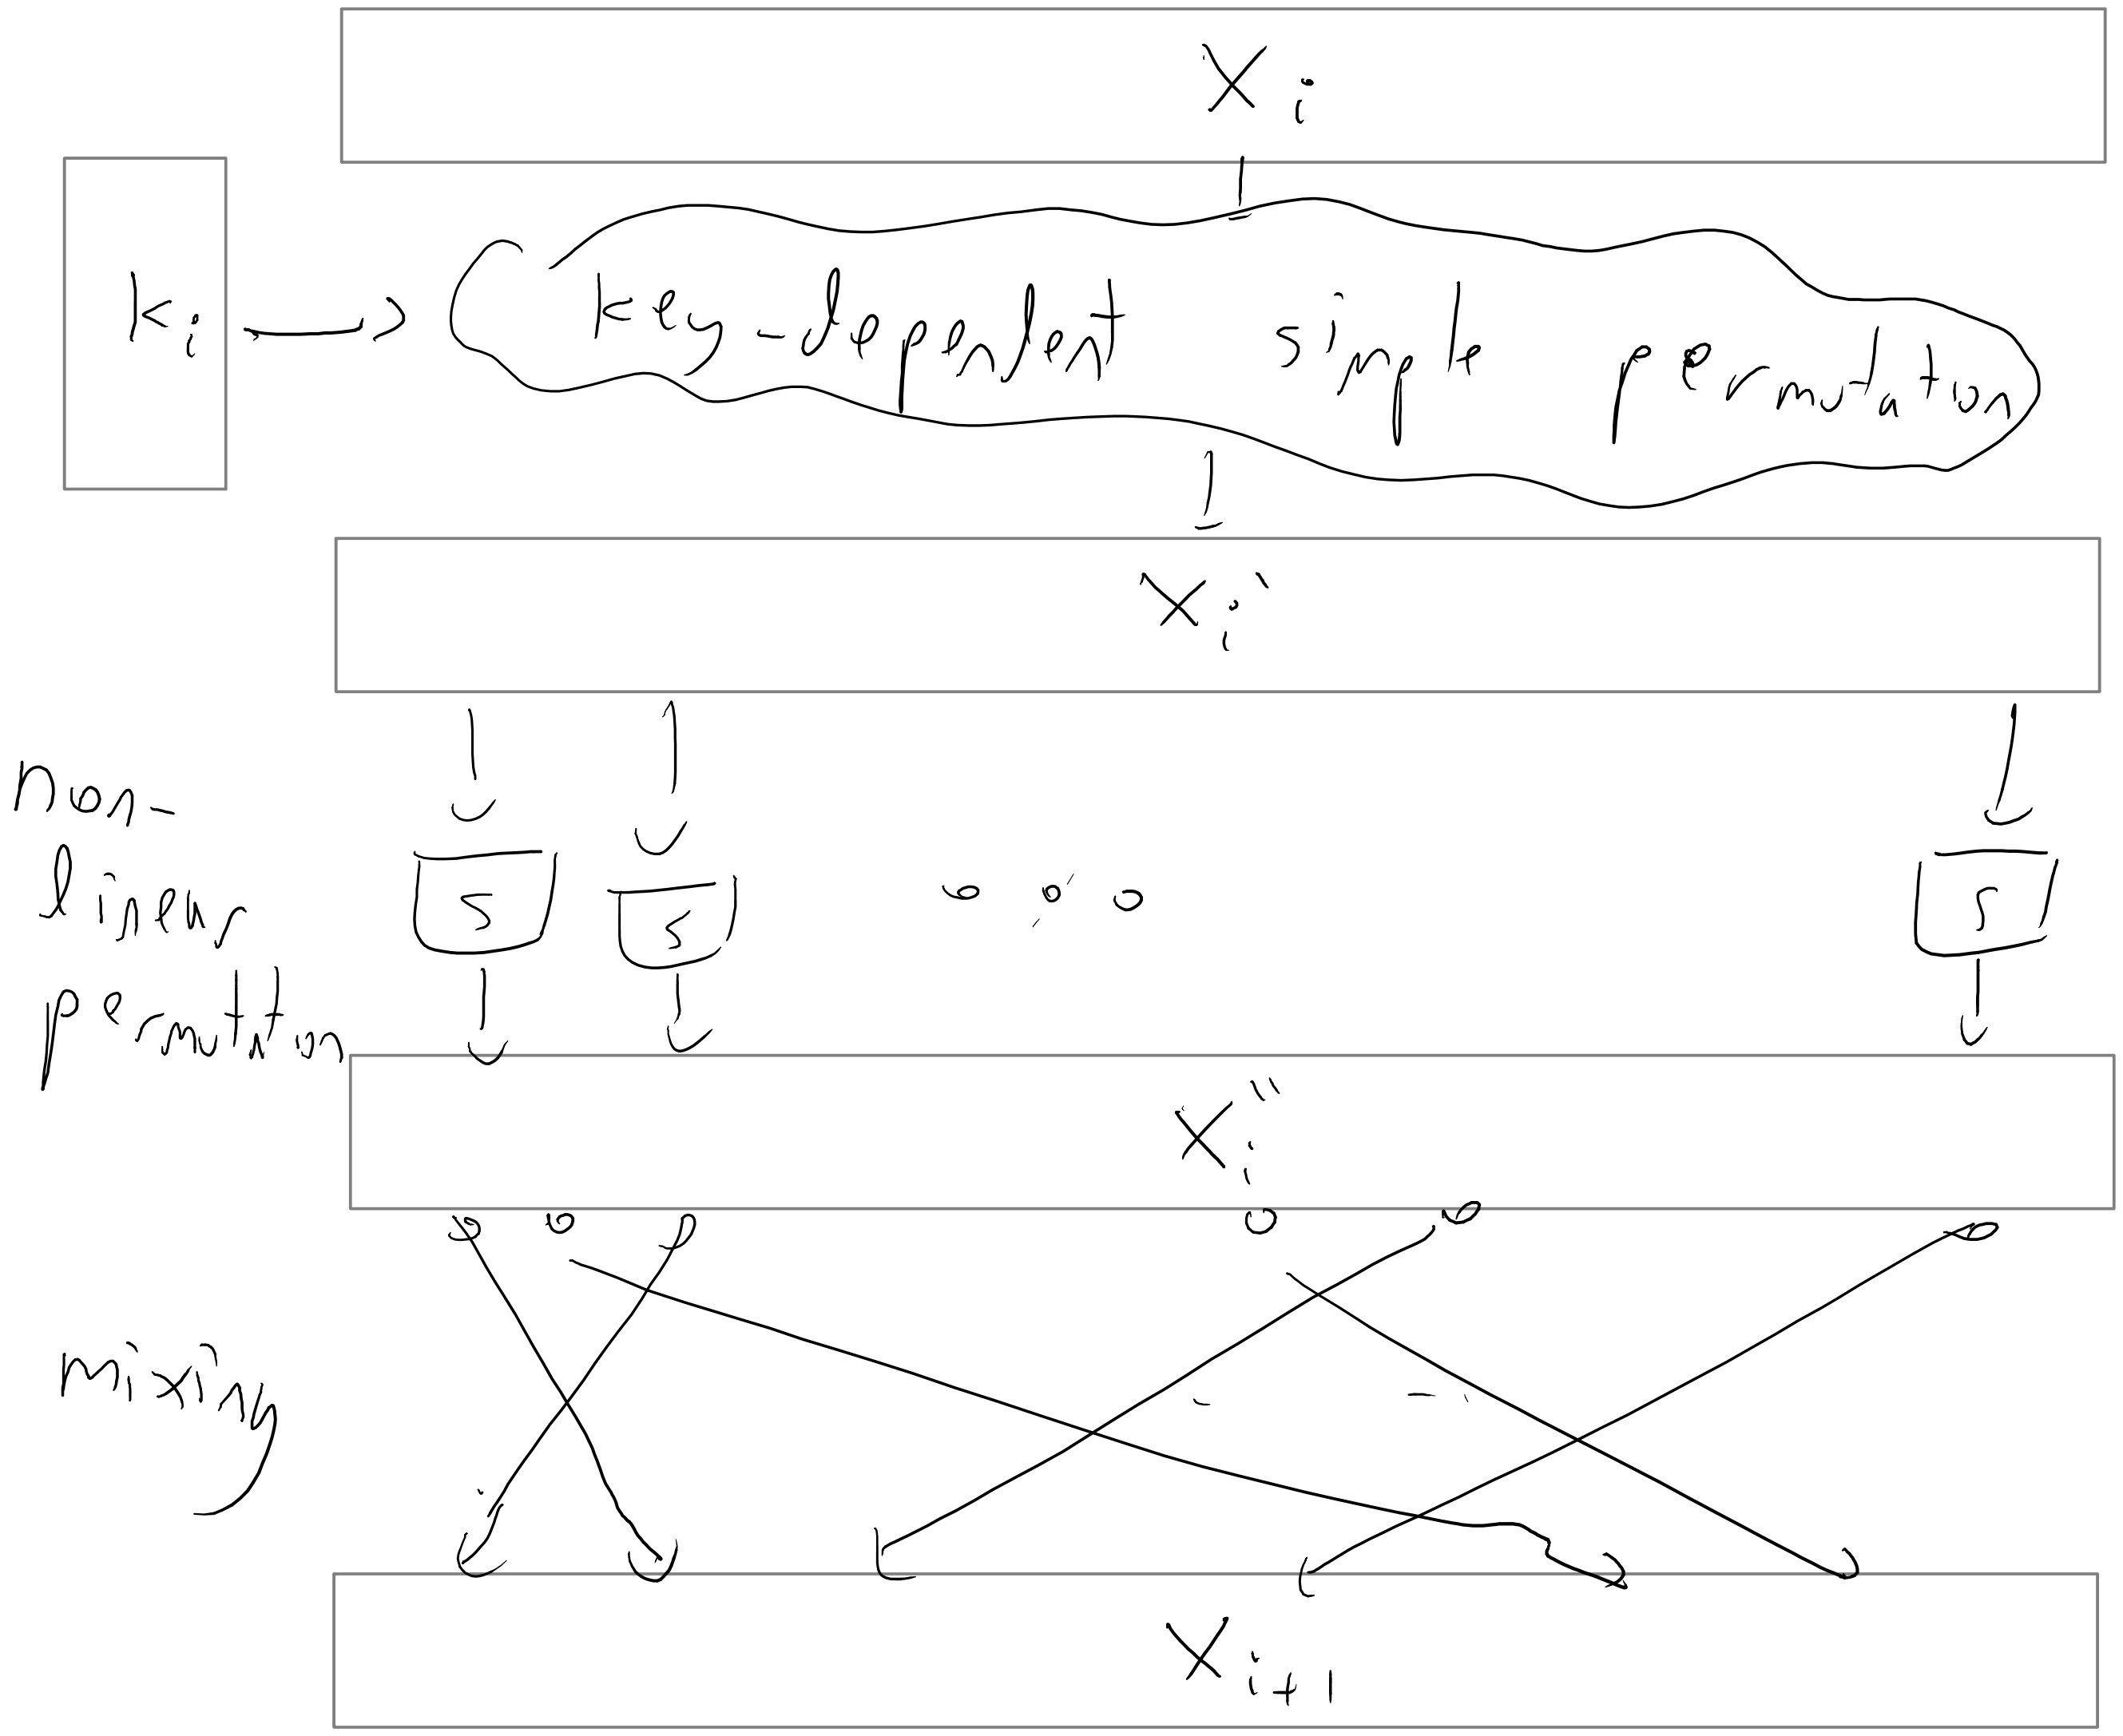
\includegraphics[width=\linewidth, height=1.5in, keepaspectratio]{../figure/block-cipher-round.jpg}
\caption{A typical round of a block cipher, \(k_i\) is the \(i^{th}\)
round key, \(x_i\) is the block before the \(i^{th}\) round and
\(x_{i+1}\) is the block at the end of this round.}
\label{blockcipherfig}
\end{marginfigure}

\section{Encryption modes}\label{5-Encryption-modes}

How do we use a block cipher to actually encrypt traffic? Well we could
use it as a PRF in the construction above, but in practice people use
other ways.\footnote{Partially this is because in the above construction
  we had to encode a plaintext of length \(n\) with a ciphertext of
  length \(2n\) meaning an overhead of 100 percent in the communication.}

The most natural approach would be that to encrypt a message \(m\), we
simply use \(p_s(m)\) where \(\{ p_s \}\) is the PRP/block cipher. This
is known as the \emph{electronic code book (ECB) mode} of a block cipher
(see \cref{ecbonefig}). Note that we can easily decrypt since we can
compute \(p_s^{-1}(m)\). If the PRP \(\{p_s\}\) only accepts inputs of a
fixed length \(\ell\), we can use ECB mode to encrypt a message \(m\)
whose length is a multiple of \(\ell\) by writing
\(m = (m_1, m_2, \ldots, m_t)\), where each block \(m_i\) has length
\(\ell\), and then encrypting each block \(m_i\) separately. The
ciphertext output by this encryption scheme is
\((p_s(m_1), \ldots, p_s(m_t))\). A major drawback of ECB mode is that
it is a \emph{deterministic} encryption scheme and hence cannot be CPA
secure. Moreover, this is actually a real problem of security on
realistic inputs (see \cref{ecbtwofig}), so ECB mode should never be
used.

\begin{marginfigure}
\centering
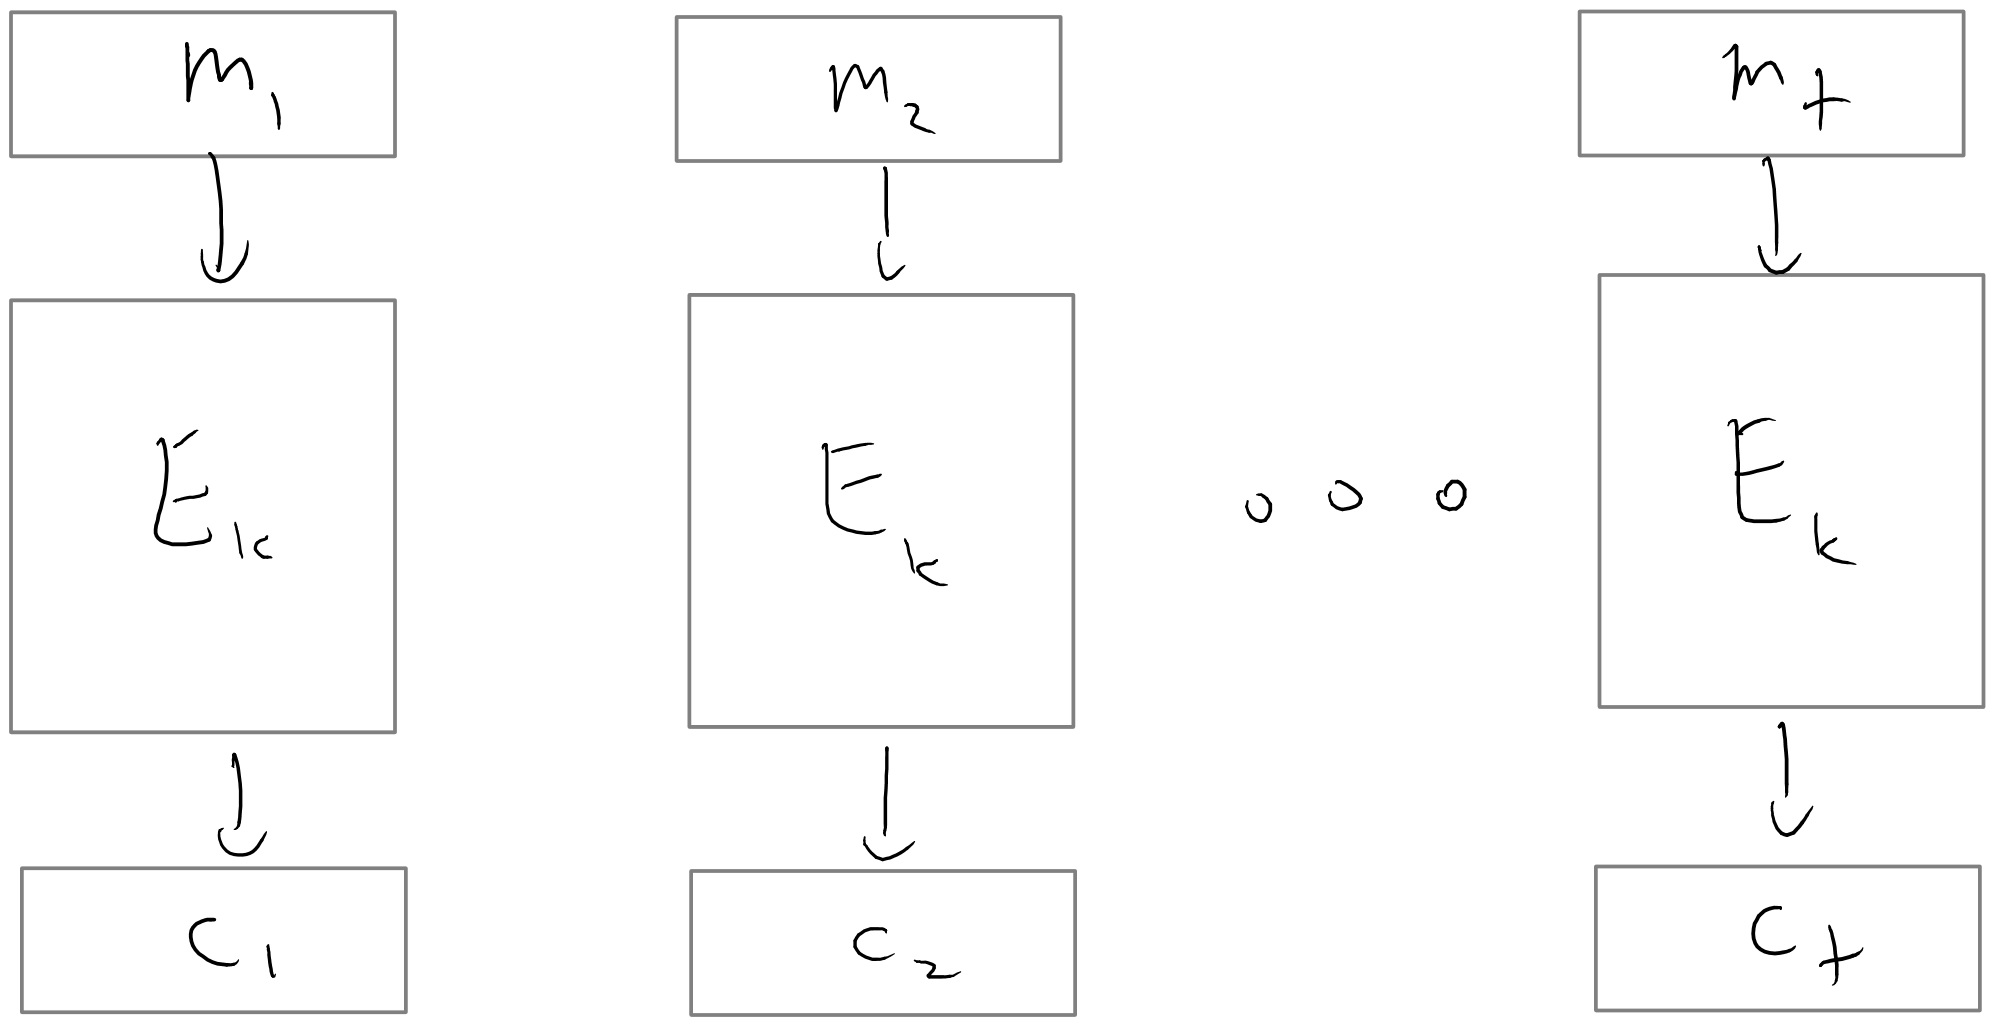
\includegraphics[width=\linewidth, height=1.5in, keepaspectratio]{../figure/ecb-mode.jpg}
\caption{In the Electronic Codebook (ECB) mode, every message is
encrypted deterministically and independently}
\label{ecbonefig}
\end{marginfigure}

\begin{marginfigure}
\centering
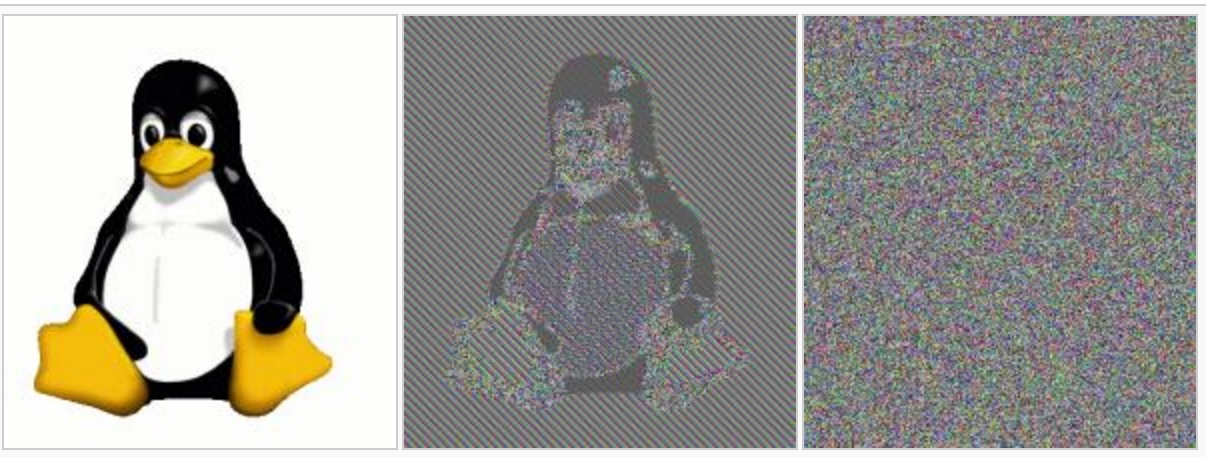
\includegraphics[width=\linewidth, height=1.5in, keepaspectratio]{../figure/ECB_prob.jpg}
\caption{An encryption of the Linux penguin (left image) using ECB mode
(middle image) vs CBC mode (right image). The ECB encryption is insecure
as it reveals much structure about the original image. Image taken from
Wikipedia.}
\label{ecbtwofig}
\end{marginfigure}

A more secure way to use a block cipher to encrypt is the \emph{cipher
block chaining (CBC) mode}. The idea of cipher block chaining is to
encrypt the blocks of a message \(m = (m_1, \ldots, m_t)\) sequentially.
To encrypt the first block \(m_1\), we XOR \(m_1\) with a random string
known as the \emph{initialization vector}, or
\(\ensuremath{\mathit{IV}}\), before applying the block cipher \(p_s\).
To encrypt one of the later blocks \(m_i\), where \(i > 1\), we XOR
\(m_i\) with the \emph{encryption} of \(m_{i-1}\) before applying the
block cipher \(p_s\). Formally, the ciphertext consists of the tuple
\((\ensuremath{\mathit{IV}}, c_1, \ldots, c_t)\), where
\(\ensuremath{\mathit{IV}}\) is chosen uniformly at random and
\(c_i = p_s(c_{i-1} \oplus m_i)\) for \(1 \le i \le t\) (we use the
convention that \(c_0 = \ensuremath{\mathit{IV}}\)). This encryption
process is depicted in \cref{cbcmodefig}. In order to decrypt
\((\ensuremath{\mathit{IV}}, c_1, \ldots, c_t)\), we simply calculate
\(m_i = p_s^{-1}(c_i) \oplus c_{i-1}\) for \(1 \le i \le t\). Note that
if we lose the block \(c_i\) to traffic in the CBC mode, then we are
unable to decrypt the next block \(c_{i+1}\), but we can recover from
that point onwards.

On the one hand, CBC mode is vastly superior to a simple electronic
codebook since CBC mode with a random \(\ensuremath{\mathit{IV}}\) is
CPA secure (proving this is an excellent exercise). On the other hand,
CBC mode suffers from the drawback that the encryption process cannot be
parallelized: the ciphertext block \(c_i\) \emph{must} be computed
before \(c_{i+1}\).

\begin{marginfigure}
\centering
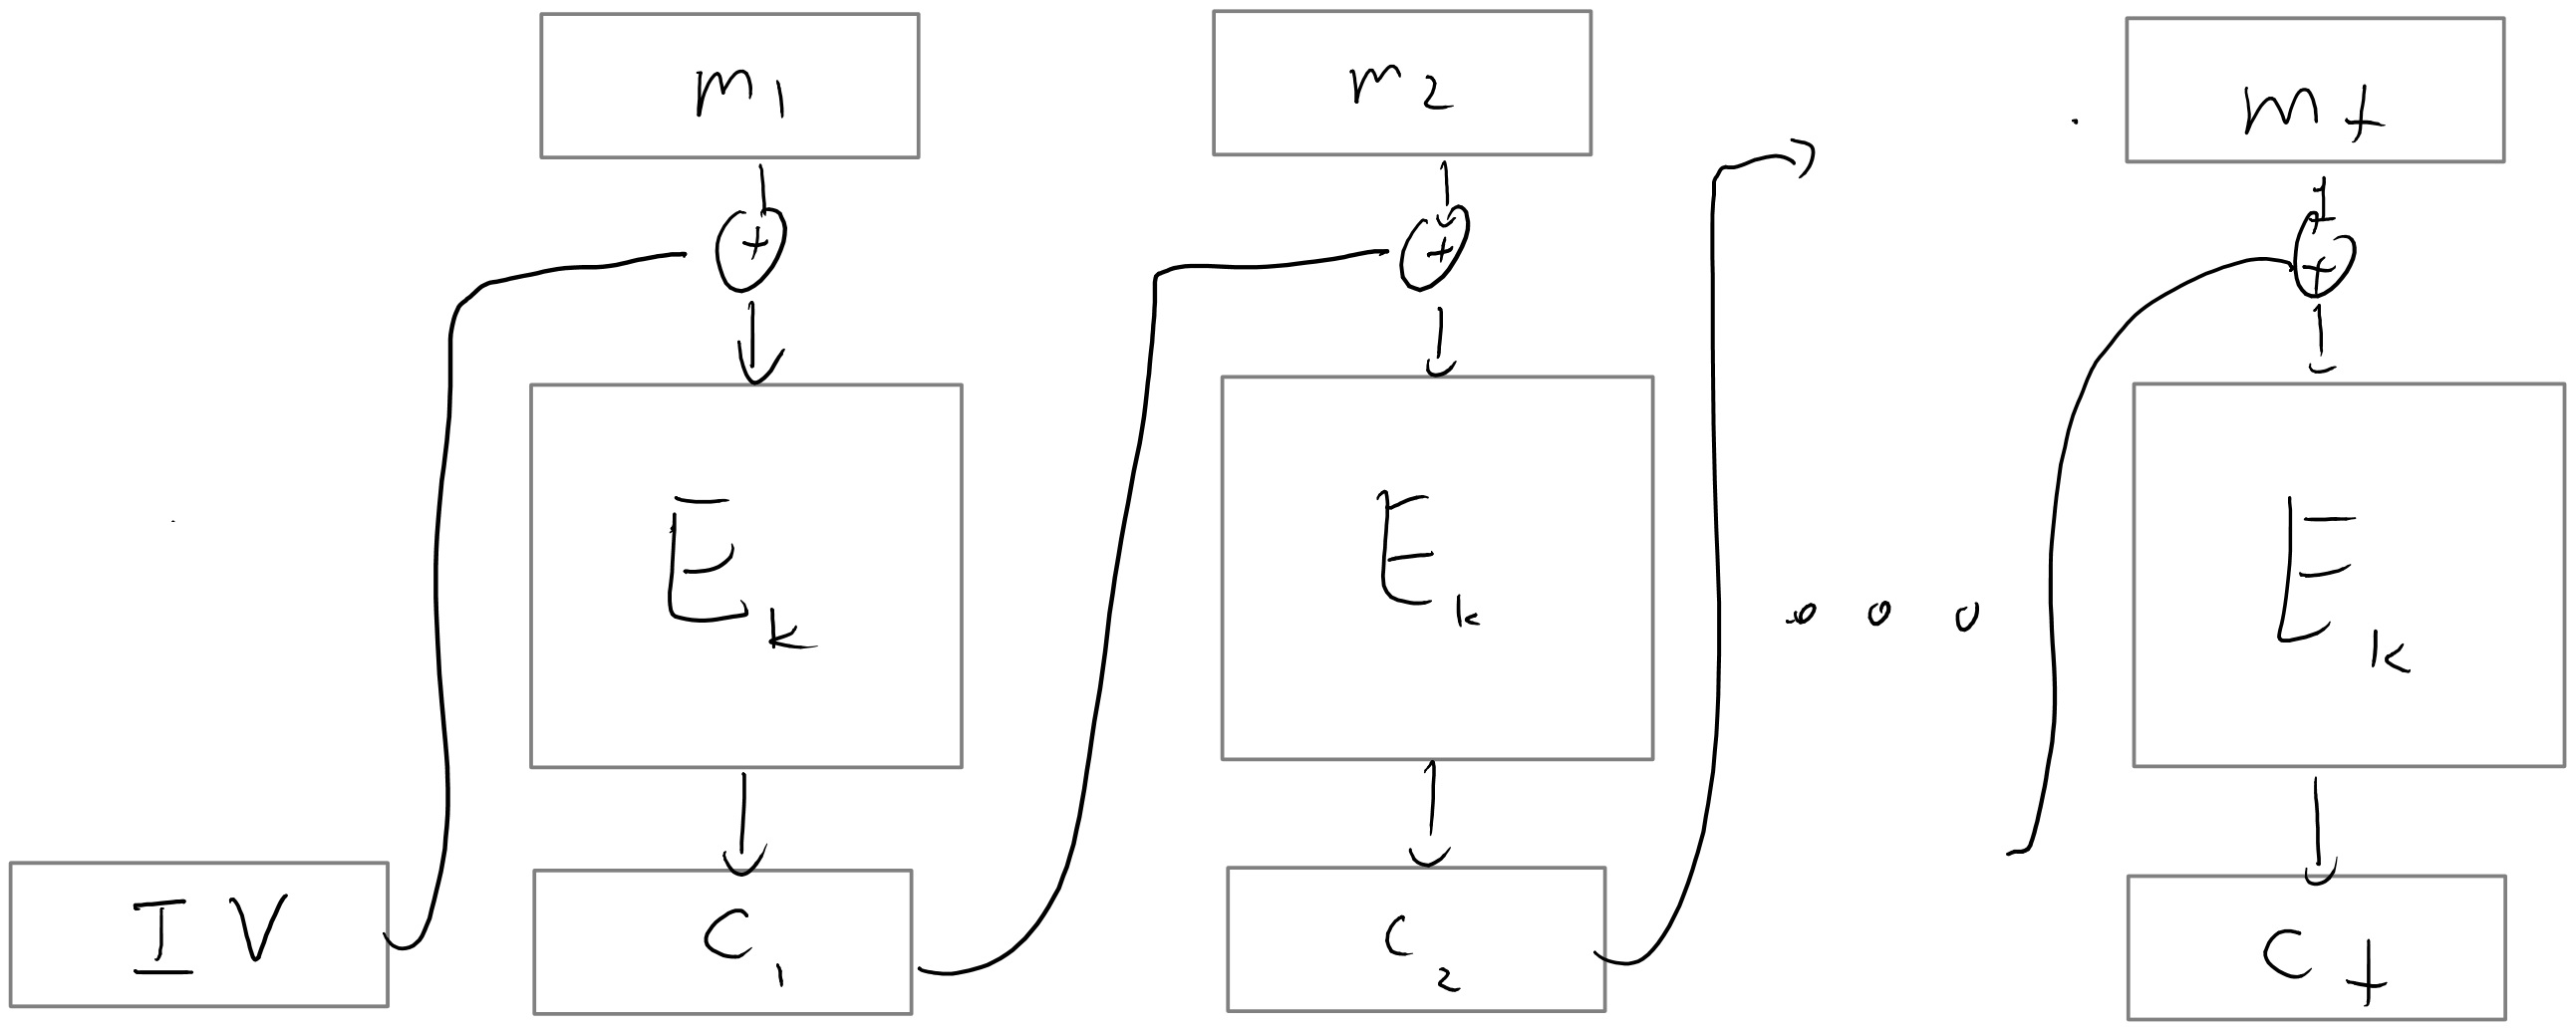
\includegraphics[width=\linewidth, height=1.5in, keepaspectratio]{../figure/cbc-mode.jpg}
\caption{In the Cypher-Block-Chaining (CBC) the encryption of the
previous message is XOR'ed into the current message prior to encrypting.
The first message is XOR'ed with an \emph{initialization vector} (IV)
that if chosen randomly, ensures CPA security.}
\label{cbcmodefig}
\end{marginfigure}

In the \emph{output feedback (OFB) mode} we first encrypt the all zero
string using CBC mode to get a sequence \((y_1,y_2,\ldots)\) of
pseudorandom outputs that we can use as a stream cipher. To transmit a
message \(m \in \{0,1\}^*\), we send the XOR of \(m\) with the bits
output by this stream cipher, along with the
\(\ensuremath{\mathit{IV}}\) used to generate the sequence. The receiver
can decrypt a ciphertext \((\ensuremath{\mathit{IV}}, c)\) by first
using \(\ensuremath{\mathit{IV}}\) to recover \((y_1, y_2, \ldots)\),
and then taking the XOR of \(c\) with the appropriate number of bits
from this sequence. Like CBC mode, OFB mode is CPA secure when
\(\ensuremath{\mathit{IV}}\) is chosen at random. Some advantages of OFB
mode over CBC mode include the ability for the sender to precompute the
sequence \((y_1, y_2, \ldots)\) well before the message to be encrypted
is known, as well as the fact that the underlying function \(p_s\) used
to generate \((y_1, y_2, \ldots)\) only needs to be a PRF (not
necessarily a PRP).

Perhaps the simplest mode of operation is \emph{counter (CTR) mode}
where we convert a block cipher to a stream cipher by using the stream
\(p_s(\ensuremath{\mathit{IV}}),p_s(\ensuremath{\mathit{IV}}+1),p_s(\ensuremath{\mathit{IV}}+2),\ldots\)
where \(\ensuremath{\mathit{IV}}\) is a random string in \(\{0,1\}^n\)
which we identify with \([2^n]\) (and perform addition modulo \(2^n\)).
That is, to encrypt a message \(m = (m_1, \ldots, m_t)\), we choose
\(\ensuremath{\mathit{IV}}\) at random, and output
\((\ensuremath{\mathit{IV}}, c_1, \ldots, c_t)\), where
\(c_i = p_s(\ensuremath{\mathit{IV}} + i) \oplus m_i\) for
\(1 \le i \le t\). Decryption is performed similarly. For a modern block
cipher, CTR mode is no less secure than CBC or OFB, and in fact offers
several advantages. For example, CTR mode can easily encrypt and decrypt
blocks in parallel, unlike CBC mode. In addition, CTR mode only needs to
evaluate \(p_s\) once to decrypt any single block of the ciphertext,
unlike OFB mode.

A fairly comprehensive study of the different modes of block ciphers is
in \href{http://web.cs.ucdavis.edu/~rogaway/papers/modes.pdf}{this
document by Rogaway}. His conclusion is that if we simply consider CPA
security (as opposed to the stronger notions of \emph{chosen ciphertext
security} we'll see in the next lecture) then counter mode is the best
choice, but CBC, OFB and CFB are widely implemented due to legacy
reasons. ECB should not be used (except as a building block as part of a
construction achieving stronger security).

\section{Optional, Aside: Broadcast
Encryption}\label{5-Optional-Aside-Broadca}

At the beginning of this chapter, we saw the proof of \cref{prfthm},
which states that the PRG Conjecture implies the existence of a secure
PRF collection. At the heart of this proof was a rather clever
construction based on a binary tree. As it turns out, similar tree
constructions have been used time and again to solve many other problems
in cryptography. In this section, we will discuss just one such
application of these tree constructions, namely \emph{broadcast
encryption}.

Let's put ourselves in the shoes of Hollywood executives facing the
following problem: we've just released a new movie for sale (in the form
of a download or a Blu-ray disc), and we'd like to prevent it from being
pirated. On the one hand, consumers who've purchased a copy of the movie
should be able to watch it on certain approved, standalone devices such
as TVs and Blu-ray players without needing an external internet
connection. On the other hand, to minimize the risk of piracy, these
consumers should \emph{not} have access to the movie data itself.

One way to protect the movie data, which we model as a string \(x\), is
to provide consumers with a secure encryption \(E_k(x)\) of the data.
Although the secret key \(k\) used to encrypt the data is hidden from
consumers, it is provided to device manufacturers so that they can embed
it in their TVs and Blu-ray players in some secure, tamper-resistant
manner. As long as the key \(k\) is never leaked to the public, this
system ensures that only approved devices can decrypt and play a
consumer's copy of the movie. For this reason, we will sometimes refer
to \(k\) as the \emph{device key}. This setup is depicted in
\cref{brdcastencfig}.

\begin{figure}
\centering
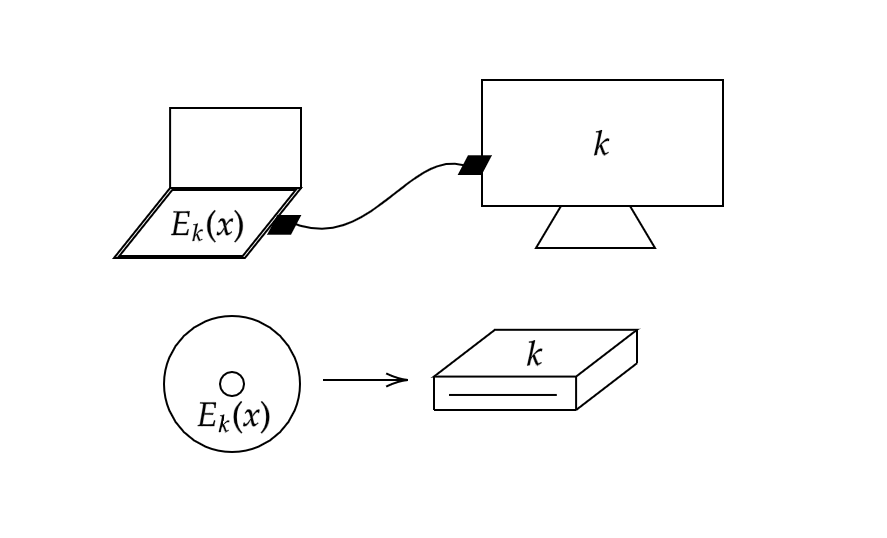
\includegraphics[width=\textwidth, height=0.25\paperheight, keepaspectratio]{../figure/brdcastencfig.png}
\caption{The problem setup for broadcast encryption.}
\label{brdcastencfig}
\end{figure}

Unfortunately, if we were to implement this scheme exactly as written,
it would almost certainly be broken in a matter of days. After all, as
soon as even a single device is hacked, the device key \(k\) would be
revealed. This would allow the public to access our movie's data, as
well as the data for \emph{all future movies} we release for these
devices! This latter consequence is one that we would certainly want to
avoid, and doing so requires the notion of distinct, \emph{revocable}
keys:

\hypertarget{broadcastdef}{}
\begin{definition}[Broadcast Encryption Scheme] \label[definition]{broadcastdef}

For our purposes, a \emph{broadcast encryption scheme} consists of:

\begin{itemize}
\item
  A set of \(m\) distinct devices (or device manufacturers), each of
  which has access to one of the \(n\)-bit device keys
  \(k_1, \ldots, k_m\).
\item
  A decryption algorithm \(D\) that receives as input a ciphertext \(y\)
  and a key \(k_i\).
\item
  An encryption algorithm \(E\) that receives as input a plaintext
  \(x\), a key \(k_{master}\), and a \emph{revocation set}
  \(R \subseteq [m]\) of devices (or device manufacturers) that are no
  longer to be trusted.
\end{itemize}

\end{definition}

Intuitively, a broadcast encryption scheme is secure if \(D_{k_i}\) can
successfully recover \(x\) from \(E_{k_{master}, R}(x)\) whenever
\(i \notin R\), but fails to do so whenever \(i \in R\). In our example
of movie piracy, such an encryption scheme would allow us to
\emph{revoke} certain device keys \(k_i\) when we find out that they
have been leaked. To revoke a key \(k_i\), we would simply include
\(i \in R\) when encrypting all future movies. Doing so prevents \(k_i\)
from being used to decrypt these movies. Crucially, revoking the key
\(k_i\) of the hacked device \(i\) doesn't prevent a secure device
\(j \neq i\) from continuing to perform decryption on future movie
releases; this is exactly what we want in our system.

For the sake of brevity, we will \emph{not} provide a formal definition
of security for broadcast encryption schemes, although this can and has
been done. Instead, in the remainder of this section, we will describe a
couple examples of broadcast encryption schemes, one of which makes
clever use of a tree construction, as promised.

The simplest construction of a broadcast encryption scheme involves
letting \(k_{master} = (k_1, \ldots, k_m)\) be the collection of all
device keys and letting \(E_{k_{master}, R}(x)\) be the concatenation
over all \(i \notin R\) of a secure encryption \(E_{k_i}(x)\). Device
\(i\) performs decryption by looking up the relevant substring
\(E_{k_i}(x)\) of the ciphertext and decrypting it with \(k_i\).
Intuitively, with this scheme, if \(x\) represents our movie data and
there are \(m \approx\) one million devices, then
\(E_{k_{master}, R}(x)\) is just an encryption of one million copies of
the movie (one for each device key). Revoking the key \(k_i\) amounts to
only encrypting \(999,999\) copies of all future movies, so that device
\(i\) can no longer perform decryption.

Clearly, this simple solution to the broadcast encryption problem has
two serious inefficiencies: the length of the master key is \(O(nm)\),
and the length of each encryption is \(O(|x|m)\). One way to address the
former problem is to use a \emph{key derivation function}. That is, we
can shorten the master key by choosing a fixed PRF collection
\(\{f_k\}\), and calculating each device key \(k_i\) by the rule
\(k_i = f_{k_{master}}(i)\). The latter problem can be addressed using a
technique known as \emph{hybrid encryption}. In hybrid encryption, we
encrypt \(x\) by first choosing an ephemeral key
\(\hat k \leftarrow_R \{0,1\}^n\), encrypting \(\hat k\) using each
device key \(k_i\) where \(i \notin R\), and then outputting the
concatenation of these strings \(E_{k_i}(\hat k)\), along with a
\emph{single} encryption \(E_{\hat k}(x)\) of the movie using the
ephermal key. Incorporating these two optimizations reduces the length
of \(k_{master}\) to \(O(n)\) and the length of each encryption to
\(O(nm + |x|)\).

\begin{figure}
\centering
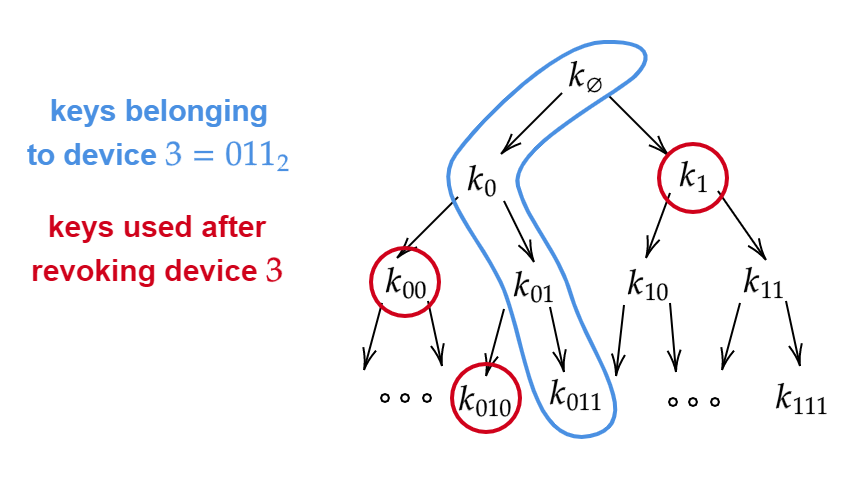
\includegraphics[width=\textwidth, height=0.25\paperheight, keepaspectratio]{../figure/brdcasttreefig.png}
\caption{A tree based construction of broadcast encryption with
revocable keys.}
\label{brdcasttreefig}
\end{figure}

It turns out that we can construct a broadcast encryption scheme with
even shorter ciphertexts by considering a \emph{tree of keys} (see
\cref{brdcasttreefig}). The root of this tree is labeled
\(k_{\varnothing}\), its children are \(k_0\) and \(k_1\), their
children are \(k_{00}, k_{01}, k_{10}, k_{11}\), and so on. The depth of
the tree is \(\log_2 m\), and the value of each key in the tree is
decided uniformly at random, or by applying a key derivation function to
a string \(k_{master}\). Each device \(i\) receives \emph{all} the keys
on the path from the root to the \(i\)th leaf. For example, if \(m=8\),
then device \(011\) receives the keys
\(k_{\varnothing}, k_0, k_{01}, k_{011}\).

To encrypt a message \(x\), we carry out the following procedure:
initially, when no keys have been revoked, we encrypt \(x\) using an
ephermal key \(\hat k\) (as described above) and encrypt \(\hat k\) with
a single device key \(k_\varnothing\). This is sufficient since all
devices have access to \(k_\varnothing\). In order to add a hacked
device \(i\) to the revocation set, we discard all \(\log_2 m\) keys
belonging to device \(i\), which comprise a root-to-leaf path in the
tree. Instead of using these keys, we will make sure to encrypt all
future \(\hat k\)'s using the \emph{siblings} of the vertices along this
path. Doing so ensures that (1) device \(i\) can no longer decrypt
secure content and (2) every device \(j \neq i\) can \emph{continue} to
decrypt content using at least one of the keys along the path from the
root to the \(j\)th leaf. With this scheme, the total length of a
ciphertext is only \(O(n|R| \log_2 m + |x|)\) bits, where \(|R|\) is the
number of devices revoked so far. When \(|R|\) is small, this bound is
\emph{much} better than what we previously achieved without a tree-based
construction.

\section{Reading comprehension
exercises}\label{5-Reading-comprehension-}

I recommend students do the following exercises after reading the
lecture. They do not cover all material, but can be a good way to check
your understanding.

\begin{exercise} \label[exercise]{5-Let-ED-be-the-encrypti}

Let \((E,D)\) be the encryption scheme that we saw in Lecture 2 where
\(E_k(m)=G(k)\oplus m\) where \(G(\cdot)\) is a pseudorandom generator.
Is this scheme CPA secure?

\begin{enumerate}
\def\labelenumi{\alph{enumi}.}
\tightlist
\item
  No it is never CPA secure.
\item
  It is always CPA secure.
\item
  It is sometimes CPA secure and sometimes not, depending on the
  properties of the PRG \(G\)
\end{enumerate}

\end{exercise}

\begin{exercise} \label[exercise]{5-Consider-the-proof-con}

Consider the proof constructing PRFs from PRGs. Up to an order of
magnitude, how many invocations of the underlying pseudorandom generator
does the pseudorandom function collection make when queried on an input
\(i\in \{0,1\}^n\)?

\begin{enumerate}
\def\labelenumi{\alph{enumi}.}
\tightlist
\item
  \(n\)
\item
  \(n^2\)
\item
  \(1\)
\item
  \(2^n\)
\end{enumerate}

\end{exercise}

\begin{exercise} \label[exercise]{5-In-the-following-we-id}

In the following we identify a block cipher with a pseudorandom
permutation (PRP) collection. Which of these statements is true:

\begin{enumerate}
\def\labelenumi{\alph{enumi}.}
\tightlist
\item
  Every PRP collection is also a PRF collection
\item
  Every PRF collection is also a PRP collection
\item
  If \(\{ f_s \}\) is a PRP collection then the encryption scheme
  \(E_s(m)=f_s(m)\) is a CPA secure encryption scheme.
\item
  If \(\{ f_s \}\) is a PRF collection then the encryption scheme
  \(E_s(m)=f_s(m)\) is a CPA secure encryption scheme.
\end{enumerate}

\end{exercise}

\chapter{Chosen Ciphertext Security}\label{Chosen-Ciphertext-Securit}

\section{Short recap}\label{Short-recap}

Let's start by reviewing what we have learned so far:

\begin{itemize}
\item
  We can mathematically define security for encryption schemes. A
  natural definition is \emph{perfect secrecy}: no matter what Eve does,
  she can't learn anything about the plaintext that she didn't know
  before. Unfortunately this requires the key to be as long as the
  message, thus placing a severe limitation on the usability of it.
\item
  To get around this, we need to consider computational considerations.
  A basic object is a \emph{pseudorandom generator} and we considered
  the \emph{PRG Conjecture} which stipulates the existence of an
  efficiently computable function
  \(G:\{0,1\}^n\rightarrow\{0,1\}^{n+1}\) such that
  \(G(U_n)\approx U_{n+1}\) (where \(U_m\) denotes the uniform
  distribution on \(\{0,1\}^m\) and \(\approx\) denotes computational
  indistinguishability).
\item
  We showed that the PRG conjecture implies a pseudorandom generator of
  any polynomial output length which in particular via the stream cipher
  construction implies a computationally secure encryption with
  plaintext arbitrarily larger than the key. (The only restriction is
  that the plaintext is of polynomial size which is needed anyway if we
  want to actually be able to read and write it.)
\item
  We then showed that the PRG conjecture actually implies a stronger
  object known as a \emph{pseudorandom function (PRF) function
  collection}: this is a collection \(\{ f_s \}\) of functions such that
  if we choose \(s\) at random and fix it, and give an adversary a black
  box computing \(i \mapsto f_s(i)\) then she can't tell the difference
  between this and a blackbox computing a random function.
\item
  Pseudorandom functions turn out to be useful for \emph{identification
  protocols}, \emph{message authentication codes} and this strong notion
  of security of encryption known as \emph{chosen plaintext attack (CPA)
  security} where we are allowed to encrypt \emph{many messages of Eve's
  choice} and still require that the next message hides all information
  except for what Eve already knew before.
\end{itemize}

\section{Going beyond CPA}\label{Going-beyond-CPA}

It may seem that we have finally nailed down the security definition for
encryption. After all, what could be stronger than allowing Eve
unfettered access to the encryption function? Clearly an encryption
satisfying this property will hide the contents of the message in all
practical circumstances. Or will it?

\begin{pause} \label[pause]{Please-stop-and-play-an-o}

Please stop and play an ominous sound track at this point.

\end{pause}

\subsection{Example: The Wired Equivalence Protocol
(WEP)}\label{Example-The-Wired-Equival}

The WEP is perhaps one of the most inaccurately named protocols of all
times. It was invented in 1999 for the purpose of securing Wi-Fi
networks so that they would have virtually the same level of security as
wired networks, but already early on several security flaws were pointed
out. In particular in 2001, Fluhrer, Mantin, and Shamir showed how the
RC4 flaws we mentioned in prior lecture can be used to completely break
WEP in less than one minute. Yet, the protocol lingered on and for many
years after was still the most widely used WiFi encryption protocol as
many routers had it as the default option. In 2007 the WEP was blamed
for a hack stealing 45 million credit card numbers from T.J. Maxx. In
2012 (after 11 years of attacks!) it was estimated that it is still used
in about a quarter of encrypted wireless networks, and in 2014 it was
still the default option on many Verizon home routers. (I don't know of
more recent surveys.) Here we will talk about a different flaw of WEP
that is in fact shared by many other protocols, including the first
versions of the secure socket layer (SSL) protocol that is used to
protect all encrypted web traffic.

To avoid superfluous details we will consider a highly abstract (and
somewhat inaccurate) version of WEP that still demonstrates our main
point. In this protocol Alice (the user) sends to Bob (the access point)
an IP packet that she wants routed somewhere on the internet.

Thus we can think of the message Alice sends to Bob as a string
\(m\in\{0,1\}^\ell\) of the form \(m=(m_1,m_2)\) where \(m_1\) is the IP
address this packet needs to be routed to and \(m_2\) is the actual
message that needs to be delivered. In the WEP protocol, the message
that Alice sends to Bob has the form\\
\(E_k(m\|\ensuremath{\mathit{CRC}}(m))\) (where \(\|\) denotes
concatenation and \(\ensuremath{\mathit{CRC}}(m)\) is some cyclic
redundancy code). The actual encryption WEP used was RC4, but for us it
doesn't really matter. What does matter is that the encryption has the
form \(E_k(m') = pad \oplus m'\) where \(pad\) is computed as some
function of the key. In particular the attack we will describe works
even if we use our stronger CPA secure PRF-based scheme where
\(pad=f_k(r)\) for some random (or counter) \(r\) that is sent out
separately.

Now the security of the encryption means that an adversary seeing the
ciphertext \(c=E_k(m\|crc(m))\) will not be able to know \(m\), but
since this is traveling over the air, the adversary could ``spoof'' the
signal and send a different ciphertext \(c'\) to Bob. In particular, if
the adversary knows the IP address \(m_1\) that Alice was using (e.g.,
for example, the adversary can guess that Alice is probably one of the
billions of people that visit the website boazbarak.org on a regular
basis) then she can XOR the ciphertext with a string of her choosing and
hence convert the ciphertext
\(c = pad \oplus (m_1,m_2,\ensuremath{\mathit{CRC}}(m_1,m_2))\) into the
ciphertext \(c' = c \oplus x\) where \(x=(x_1,x_2,x_3)\) is computed so
that \(x_1 \oplus m_1\) is equal to the adversary's own IP address!

So, the adversary doesn't need to decrypt the message- by spoofing the
ciphertext she can ensure that Bob (who is an access point, and whose
job is to decrypt and then deliver packets) simply delivers it
unencrypted straight into her hands. One issue is that Eve modifies
\(m_1\) then it is unlikely that the CRC code will still check out, and
hence Bob would reject the packet. However,
\href{https://goo.gl/5aqEHB}{CRC 32} - the CRC algorithm used by WEP -
is \emph{linear} modulo \(2\), which means that for every pair of
strings \(x_1,x_2\),
\(\ensuremath{\mathit{CRC}}(m_1\oplus x_1,m_2 \oplus m_2)=\ensuremath{\mathit{CRC}}(m_1,m_2)\oplus \ensuremath{\mathit{CRC}}(x_1,x_2)\).
This means that if the original ciphertext \(c\) was an encryption of
the message \(m=(m_1,m_2,\ensuremath{\mathit{CRC}}(m_1,m_2))\) then
\(c'=c \oplus (x_1,0,\ensuremath{\mathit{CRC}}(x_1,0))\) will be an
encryption of the message
\(m'=(m_1 \oplus x_1, m_2, \ensuremath{\mathit{CRC}}(x_1\oplus m_1,m_2))\)
(where \(0\) denotes a string of zeroes of the same length as \(m_2\),
and hence \(m_2 \oplus 0 = m_2\)). Therefore by XOR'ing \(c\) with
\((x_1,0,\ensuremath{\mathit{CRC}}(x_1,0))\), the adversary Mallory can
ensure that Bob will deliver the message \(m_2\) to the IP address
\(m_1 \oplus x_1\) of her choice (see \cref{WEPattackfig}).


\begin{figure}
\centering
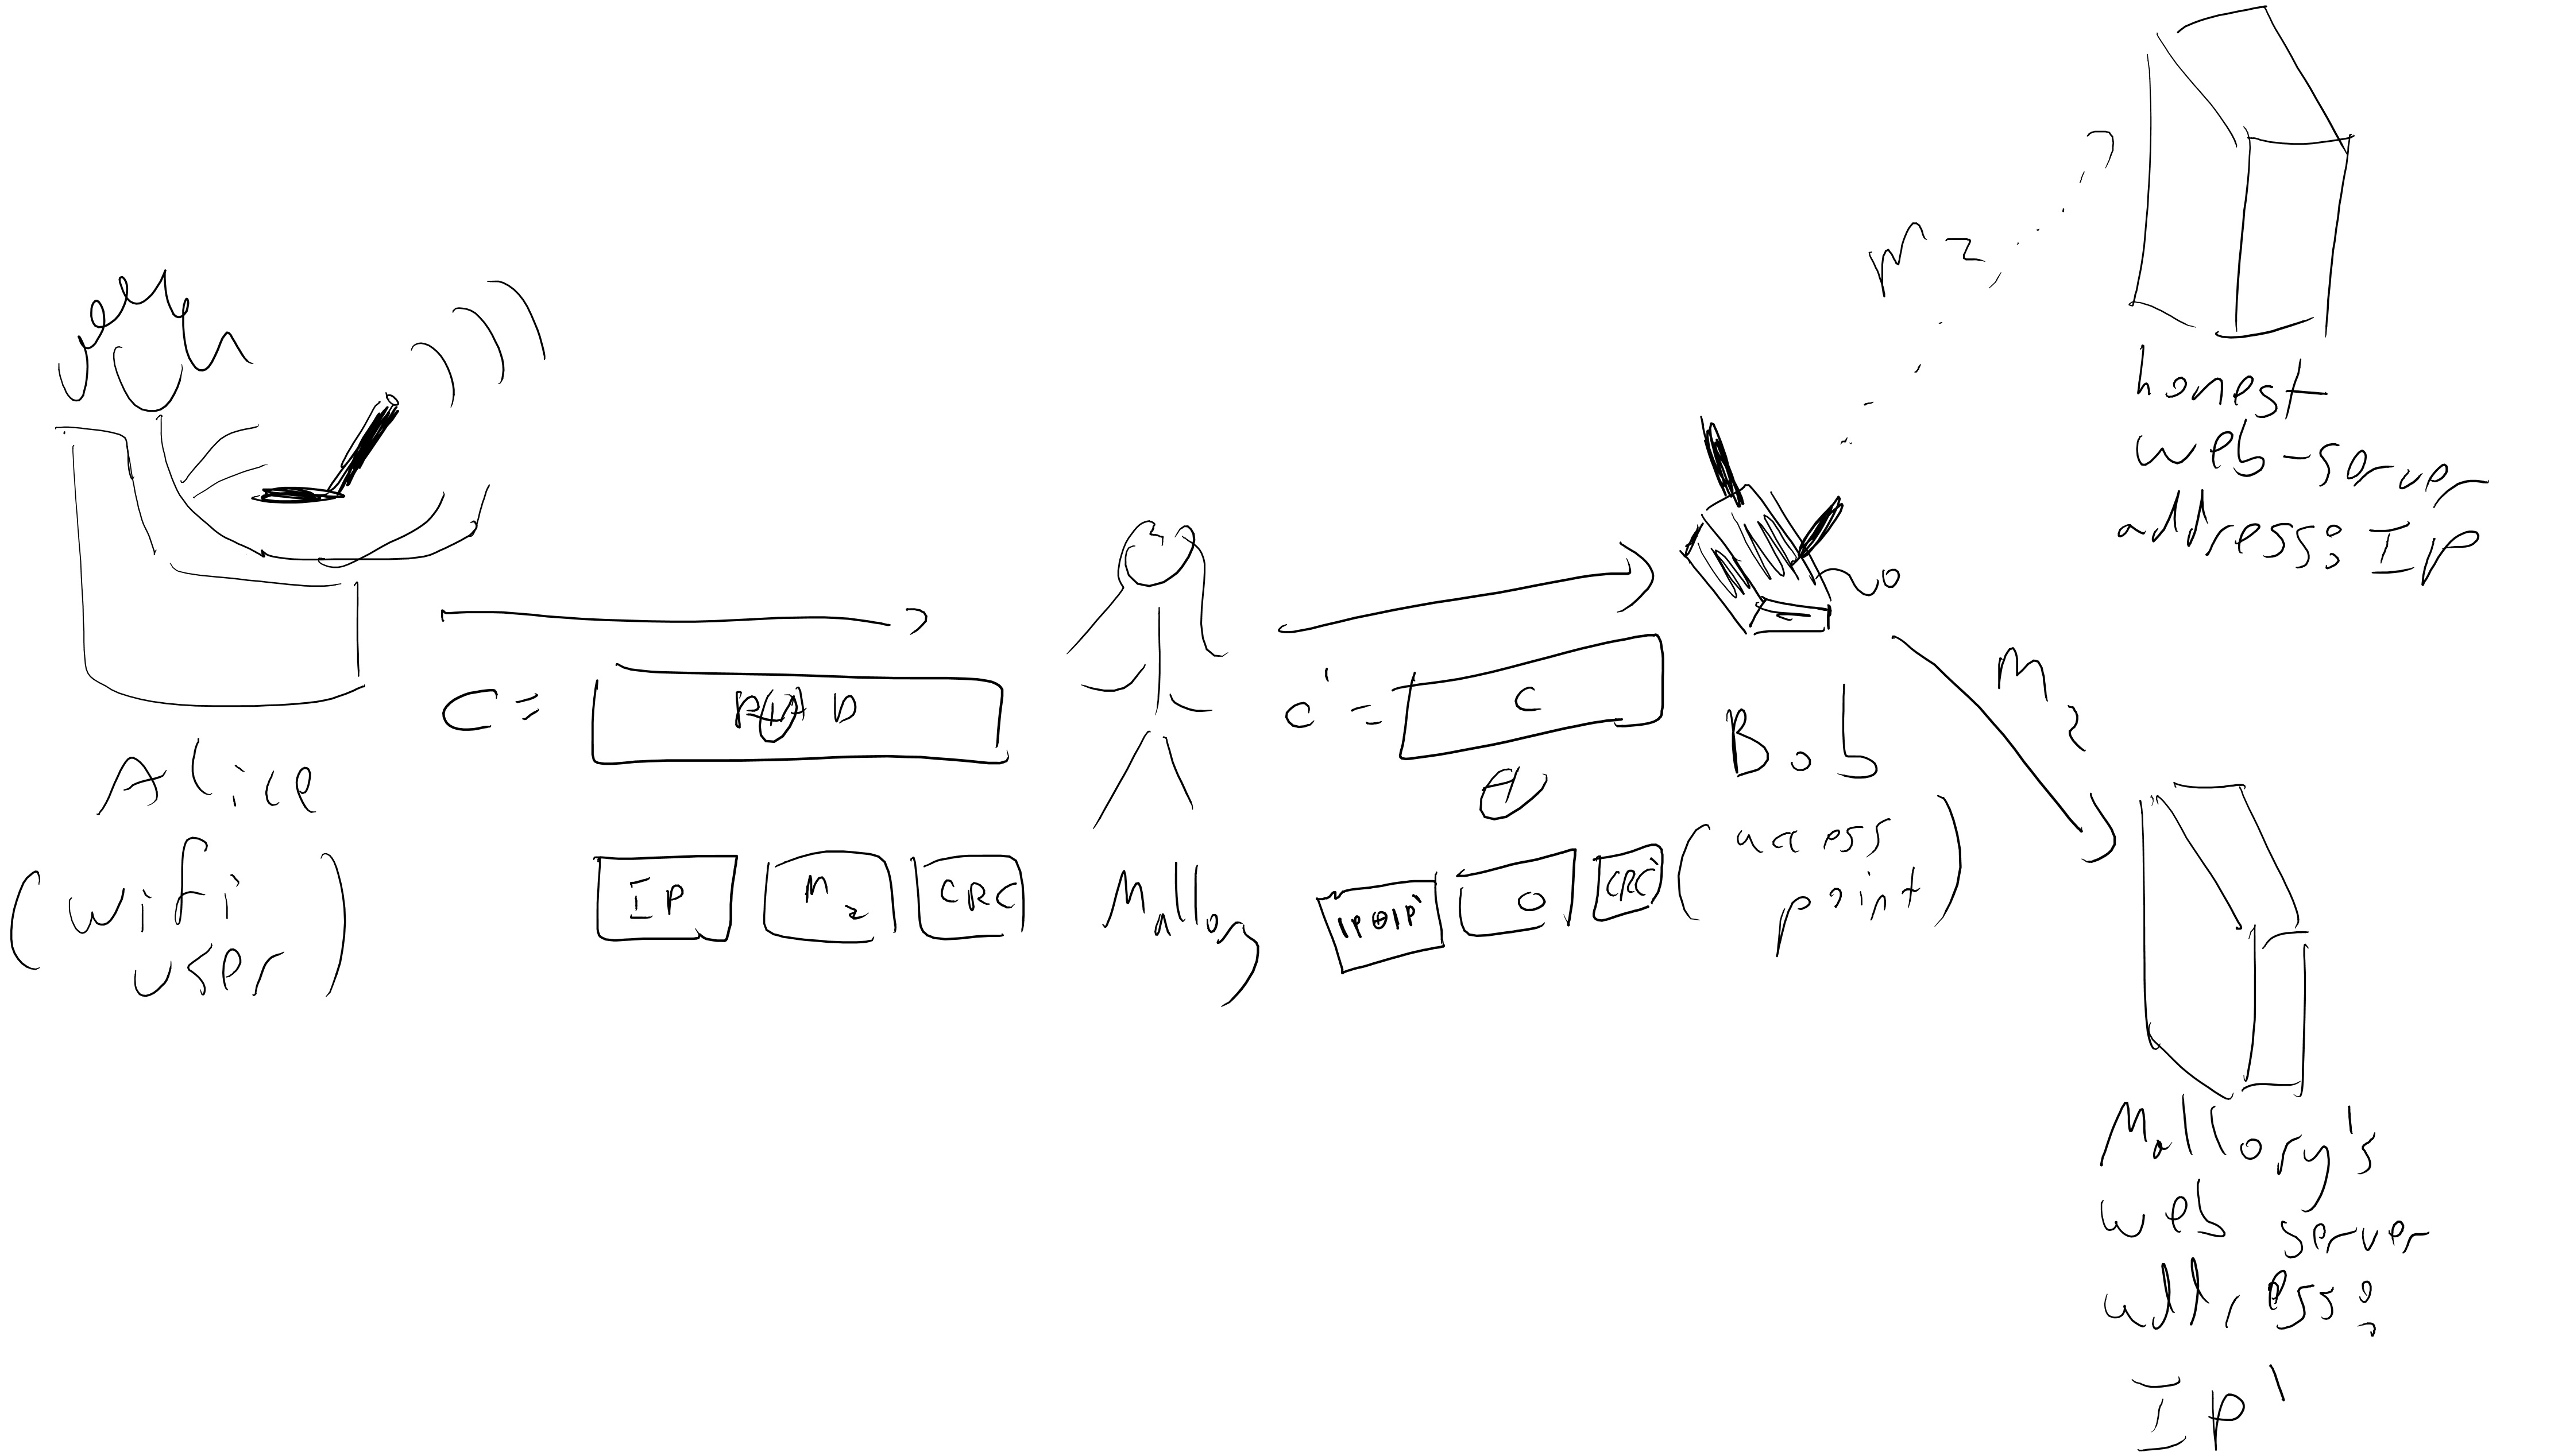
\includegraphics[width=\textwidth, height=0.25\paperheight, keepaspectratio]{../figure/wep-attack.jpg}
\caption{The attack on the WEP protocol allowing the adversary Mallory
to read encrypted messages even when Alice uses a CPA secure
encryption.}
\label{WEPattackfig}
\end{figure}

\subsection{Chosen ciphertext security}\label{Chosen-ciphertext-securit}

This is not an isolated example but in fact an instance of a general
pattern of many breaks in practical protocols. Some examples of
protocols broken through similar means include
\href{http://www.nds.rub.de/media/nds/veroeffentlichungen/2011/10/22/HowToBreakXMLenc.pdf}{XML
encryption},
\href{https://www.cs.columbia.edu/~smb/papers/badesp.pdf}{IPSec} (see
also \href{https://eprint.iacr.org/2005/416}{here}) as well as
JavaServer Faces, Ruby on Rails, ASP.NET, and the Steam gaming client
(see the Wikipedia page on \href{https://goo.gl/b5aKYg}{Padding Oracle
Attacks}).

The point is that often our adversaries can be \emph{active} and modify
the communication between sender and receiver, which in effect gives
them access not just to choose \emph{plaintexts} of their choice to
encrypt but even to have some impact on the \emph{ciphertexts} that are
decrypted. This motivates the following notion of security (see also
\cref{CCAgamefig}):

\hypertarget{CCAdef}{}
\begin{definition}[CCA security] \label[definition]{CCAdef}

An encryption scheme \((E,D)\) is \emph{chosen ciphertext attack (CCA)
secure} if every efficient adversary \emph{Mallory} wins in the
following game with probability at most \(1/2+ negl(n)\):\\
* Mallory gets \(1^n\) where \(n\) is the length of the key\\
* For \(poly(n)\) rounds, Mallory gets access to the functions
\(m \mapsto E_k(m)\) and \(c \mapsto D_k(c)\).\\
* Mallory chooses a pair of messages \(\{ m_0,m_1 \}\), a secret \(b\)
is chosen at random in \(\{0,1\}\), and Mallory gets
\(c^* = E_k(m_b)\).\\
* Mallory now gets another \(poly(n)\) rounds of access to the functions
\(m \mapsto E_k(m)\) and \(c \mapsto D_k(c)\) except that she is not
allowed to query \(c^*\) to her second oracle.\\
* Mallory outputs \(b'\) and \emph{wins} if \(b'=b\).

\end{definition}


\begin{marginfigure}
\centering
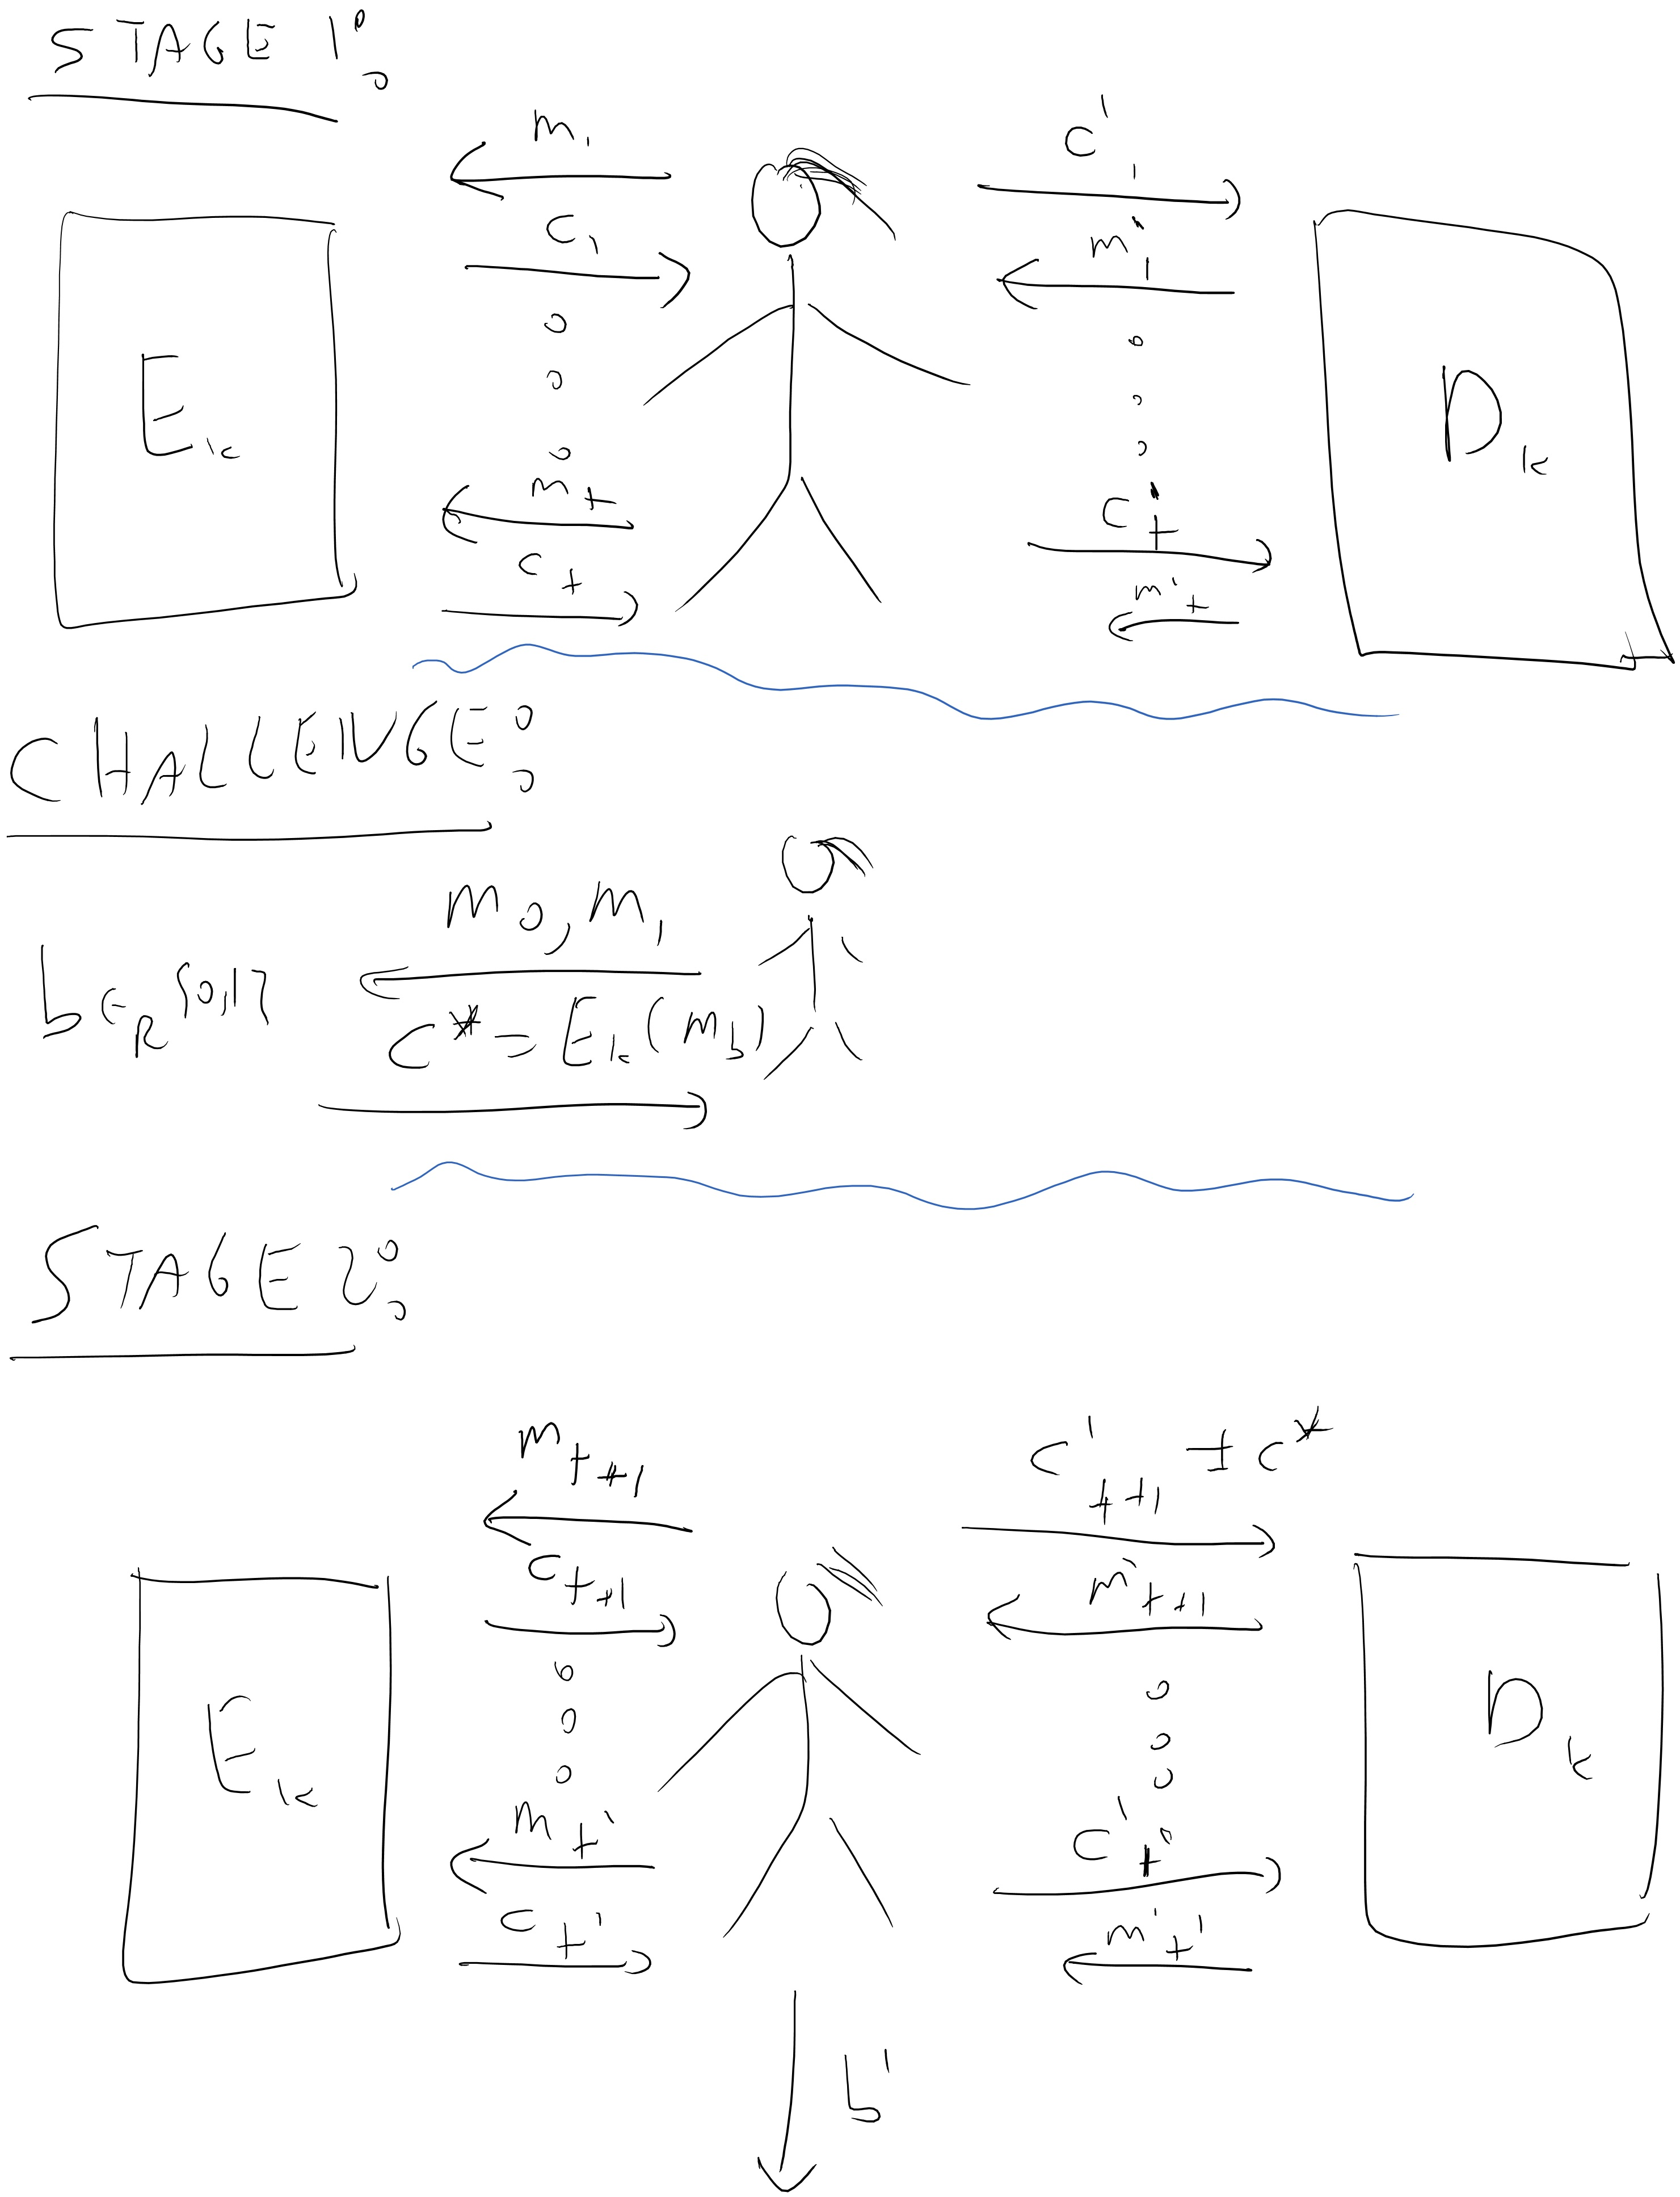
\includegraphics[width=\linewidth, height=1.5in, keepaspectratio]{../figure/cca-game.jpg}
\caption{The CCA security game.}
\label{CCAgamefig}
\end{marginfigure}

This might seems a rather strange definition so let's try to digest it
slowly. Most people, once they understand what the definition says,
don't like it that much. There are two natural objections to it:

\begin{itemize}
\tightlist
\item
  \textbf{This definition seems to be too strong:} There is no way we
  would let Mallory play with a \emph{decryption box} - that basically
  amounts to letting her break the encryption scheme. Sure, she could
  have some impact on the ciphertexts that Bob decrypts and observe some
  resulting side effects, but there is a long way from that to giving
  her oracle access to the decryption algorithm.
\end{itemize}

The response to this is that it is very hard to model what is the
``realistic'' information Mallory might get about the ciphertexts she
might cause Bob to decrypt. The goal of a security definition is not to
capture exactly the attack scenarios that occur in real life but rather
to be \emph{sufficiently conservative} so that these real life attacks
could be modeled in our game. Therefore, having a too strong definition
is not a bad thing (as long as it can be achieved!). The WEP example
shows that the definition does capture a practical issue in security and
similar attacks on practical protocols have been shown time and again
(see for example the discussion of ``padding attacks'' in Section 3.7.2
of the Katz Lindell book.)

\begin{itemize}
\tightlist
\item
  \textbf{This definition seems to be too weak:} What justification do
  we have for not allowing Mallory to make the query \(c^*\) to the
  decryption box? After all she is an adversary so she could do whatever
  she wants. The answer is that the definition would be clearly
  impossible to achieve if Mallory could simply get the decryption of
  \(c^*\) and learn whether it was an encryption of \(m_0\) or \(m_1\).
  So this restriction is the absolutely minimal one we could make
  without causing the notion to be obviously impossible. Perhaps
  surprisingly, it turns out that once we make this minimal restriction,
  we can in fact construct CCA-secure encryptions.
\end{itemize}

\paragraph{What does CCA have to do with WEP?} The CCA security game is
somewhat strange, and it might not be immediately clear whether it has
anything to do with the attack we described on the WEP protocol.
However, it turns out that using a CCA secure encryption \emph{would}
have prevented that attack. The key is the following claim:

\hypertarget{ccaweplem}{}
\begin{lemma} \label[lemma]{ccaweplem}

Suppose that \((E,D)\) is a CCA secure encryption. Then, there is no
efficient algorithm that given an encryption \(c\) of the plaintext
\((m_1,m_2)\) outputs a ciphertext \(c'\) that decrypts to
\((m'_1,m_2)\) where \(m'_1\neq m_1\).

\end{lemma}

In particular \cref{ccaweplem} rules out the attack of transforming
\(c\) that encrypts a message starting with a some address
\(\ensuremath{\mathit{IP}}\) to a ciphertext that starts with a
different address \(\ensuremath{\mathit{IP}}'\). Let us now sketch its
proof.

\begin{proof} \label[proof]{Well-show-that-such-if-we}

We'll show that such if we had an adversary \(M'\) that violates the
conclusion of the claim, then there is an adversary \(M\) that can win
in the CCA game.

The proof is simple and relies on the crucial fact that the CCA game
allows \(M\) to query the decryption box on \emph{any} ciphertext of her
choice, as long as it's not \emph{exactly identical} to the challenge
cipertext \(c^*\). In particular, if \(M'\) is able to morph an
encryption \(c\) of \(m\) to some encryption \(c'\) of some different
\(m'\) that agrees with \(m\) on some set of bits, then \(M\) can do the
following: in the security game, use \(m_0\) to be some random message
and \(m_1\) to be this plaintext \(m\). Then, when receiving \(c^*\),
apply \(M'\) to it to obtain a ciphertext \(c'\) (note that if the
plaintext differs then the ciphertext must differ also; can you see
why?) ask the decryption box to decrypt it and output \(1\) if the
resulting message agrees with \(m\) in the corresponding set of bits
(otherwise output a random bit). If \(M'\) was successful with
probability \(\epsilon\), then \(M\) would win in the CCA game with
probability at least \(1/2 + \epsilon/10\) or so.

\end{proof}

\begin{pause} \label[pause]{The-proof-above-is-rather}

The proof above is rather sketchy. However it is not very difficult and
proving \cref{ccaweplem} on your own is an excellent way to ensure
familiarity with the definition of CCA security.

\end{pause}

\section{Constructing CCA secure
encryption}\label{Constructing-CCA-secure-e}

The definition of CCA seems extremely strong, so perhaps it is not
surprising that it is useful, but can we actually construct it? The WEP
attack shows that the CPA secure encryption we saw before (i.e.,
\(E_k(m)=(r,f_k(r)\oplus m)\)) is \emph{not} CCA secure. We will see
other examples of \emph{non} CCA secure encryptions in the exercises.
So, how \emph{do} we construct such a scheme? The WEP attack actually
already hints of the crux of CCA security. We want to ensure that
Mallory is not able to modify the challenge ciphertext \(c^*\) to some
related \(c'\). Another way to say it is that we need to ensure the
\emph{integrity} of messages to achieve their \emph{confidentiality} if
we want to handle \emph{active} adversaries that might modify messages
on the channel. Since in in a great many practical scenarios, an
adversary might be able to do so, this is an important message that
deserves to be repeated:

\begin{quote}
\emph{To ensure confidentiality, you need integrity.}
\end{quote}

This is a lesson that has been time and again been shown and many
protocols have been broken due to the mistaken belief that if we only
care about \emph{secrecy}, it is enough to use only \emph{encryption}
(and one that is only CPA secure) and there is no need for
\emph{authentication}.
\href{http://blog.cryptographyengineering.com/2012/05/how-to-choose-authenticated-encryption.html}{Matthew
Green} writes this more provocatively as

\begin{quote}
\emph{Nearly all of the symmetric encryption modes you learned about in
school, textbooks, and Wikipedia are (potentially) insecure.\footnote{I
  also like the part where Green says about a block cipher mode that
  ``if OCB was your kid, he'd play three sports and be on his way to
  Harvard.'' We will have an exercise about a simplified version of the
  GCM mode (which perhaps only plays a single sport and is on its way to
  \ldots). You can read about OCB in Exercise 9.14 in the Boneh-Shoup
  book; it uses the notion of a ``tweakable block cipher'' which simply
  means that given a single key \(k\), you actually get a set
  \(\{ p_{k,1},\ldots,p_{k,t} \}\) of permutations that are
  indistinguishable from \(t\) independent random permutation (the set
  \(\{1,\ldots, t\}\) is called the set of ``tweaks'' and we sometimes
  index it using strings instead of numbers).}}
\end{quote}

exactly because these basic modes only ensure security for
\emph{passive} eavesdropping adversaries and do not ensure chosen
ciphertext security which is the ``gold standard'' for online
applications. (For symmetric encryption people often use the name
``authenticated encryption'' in practice rather than CCA security; those
are not identical but are extremely related notions.)

All of this suggests that Message Authentication Codes might help us get
CCA security. This turns out to be the case. But one needs to take some
care exactly \emph{how} to use MAC's to get CCA security. At this point,
you might want to stop and think how you would do this\ldots{}

\begin{pause} \label[pause]{You-should-stop-here-and-}

You should stop here and try to think how you would implement a CCA
secure encryption by combining MAC's with a CPA secure encryption.

\end{pause}

\newpage

\begin{pause} \label[pause]{If-you-didnt-stop-before-}

If you didn't stop before, then you should really stop and think now.

\end{pause}

\newpage

OK, so now that you had a chance to think about this on your own, we
will describe one way that works to achieve CCA security from MACs. We
will explore other approaches that may or may not work in the exercises.

\hypertarget{CCAfromCPAMACthm}{}
\begin{theorem}[CCA from CPA and MAC] \label[theorem]{CCAfromCPAMACthm}

Let \((E,D)\) be CPA-secure encryption scheme and \((S,V)\) be a
CMA-secure MAC with \(n\) bit keys and a canonical verification
algorithm.\footnote{By a \emph{canonical verification algorithm} we mean
  that \(V_k(m,\sigma)=1\) iff \(S_k(m)=\sigma\).} Then the following
encryption \((E',D')\) with keys \(2n\) bits is CCA secure:\\
* \(E'_{k_1,k_2}(m)\) is obtained by computing \(c=E_{k_1}(m)\) ,
\(\sigma = S_{k_2}(c)\) and outputting \((c,\sigma)\).\\
* \(D'_{k_1,k_2}(c,\sigma)\) outputs nothing (e.g., an error message) if
\(V_{k_2}(c,\sigma)\neq 1\), and otherwise outputs \(D_{k_1}(c)\).

\end{theorem}

\begin{proof} \label[proof]{Suppose-for-the-sake-of-c}

Suppose, for the sake of contradiction, that there exists an adversary
\(M'\) that wins the CCA game for the scheme \((E',D')\) with
probability at least \(1/2+\epsilon\). We consider the following two
cases:

\textbf{Case I:} With probability at least \(\epsilon/10\), at some
point during the CCA game, \(M'\) sends to its decryption box a
ciphertext \((c,\sigma)\) that is not identical to one of the
ciphertexts it previously obtained from its encryption box, and obtains
from it a non-error response.

\textbf{Case II:} The event above happens with probability smaller than
\(\epsilon/10\).

We will derive a contradiction in either case. In the first case, we
will use \(M'\) to obtain an adversary that breaks the MAC \((S,V)\),
while in the second case, we will use \(M'\) to obtain an adversary that
breaks the CPA-security of \((E,D)\).

Let's start with Case I: When this case holds, we will build an
adversary \(F\) (for ``forger'') for the MAC \((S,V)\), we can assume
the adversary \(F\) has access to the both signing and verification
algorithms as black boxes for some unknown key \(k_2\) that is chosen at
random and fixed.\footnote{Since we use a MAC with canonical
  verification, access to the signature algorithm implies access to the
  verification algorithm.} \(F\) will choose \(k_1\) on its own, and
will also choose at random a number \(i_0\) from \(1\) to \(T\), where
\(T\) is the total number of queries that \(M'\) makes to the decryption
box. \(F\) will run the entire CCA game with \(M'\), using \(k_1\) and
its access to the black boxes to execute the decryption and decryption
boxes, all the way until just before \(M'\) makes the \(i_0^{th}\) query
\((c,\sigma)\) to its decryption box. At that point, \(F\) will output
\((c,\sigma)\). We claim that with probability at least
\(\epsilon/(10T)\), our forger will succeed in the CMA game in the sense
that \textbf{(i)} the query \((c,\sigma)\) will pass verification, and
\textbf{(ii)} the message \(c\) was not previously queried before to the
signing oracle.

Indeed, because we are in Case I, with probability \(\epsilon/10\), in
this game \emph{some} query that \(M'\) makes will be one that was not
asked before and hence was \emph{not} queried by \(F\) to its signing
oracle, and moreover, the returned message is not an error message, and
hence the signature passes verification. Since \(i_0\) is random, with
probability \(\epsilon/(10T)\) this query will be at the \(i_0^{th}\)
round. Let us assume that this above event
\(\ensuremath{\mathit{GOOD}}\) happened in which the \(i_0\)-th query to
the decryption box is a pair \((c,\sigma)\) that both passes
verification and the pair \((c,\sigma)\) was not returned before by the
encryption oracle. Since we pass (canonical) verification, we know that
\(\sigma=S_{k_2}(c)\), and because all encryption queries return pairs
of the form \((c',S_{k_2}(\sigma'))\), this means that no such query
returned \(c\) as its first element either. In other words, when the
event \(\ensuremath{\mathit{GOOD}}\) happens the \(i_0\)-the query
contains a pair \((c,\sigma)\) such that \(c\) was not queried before to
the signature box, but \((c,\sigma)\) passes verification. This is the
definition of breaking \((S,V)\) in a chosen message attack, and hence
we obtain a contradiction to the CMA security of \((S,V)\).

Now for Case II: In this case, we will build an adversary \(Eve\) for
CPA-game in the original scheme \((E,D)\). As you might expect, the
adversary \(Eve\) will choose by herself the key \(k_2\) for the MAC
scheme, and attempt to play the CCA security game with \(M'\). When
\(M'\) makes \emph{encryption queries} this should not be a problem-
\(Eve\) can forward the plaintext \(m\) to its encryption oracle to get
\(c=E_{k_1}(m)\) and then compute \(\sigma = S_{k_2}(c)\) since she
knows the signing key \(k_2\).

However, what does \(Eve\) do when \(M'\) makes \emph{decryption}
queries? That is, suppose that \(M'\) sends a query of the form
\((c,\sigma)\) to its decryption box. To simulate the algorithm \(D'\),
\(Eve\) will need access to a \emph{decryption box} for \(D\), but she
doesn't get such a box in the CPA game (This is a subtle point- please
pause here and reflect on it until you are sure you understand it!)

To handle this issue \(Eve\) will follow the common approach of
``winging it and hoping for the best''. When \(M'\) sends a query of the
form \((c,\sigma)\), \(Eve\) will first check if it happens to be the
case that \((c,\sigma)\) was returned before as an answer to an
encryption query \(m\). In this case \(Eve\) will breathe a sigh of
relief and simply return \(m\) to \(M'\) as the answer. (This is
obviously correct: if \((c,\sigma)\) is the encryption of \(m\) then
\(m\) is the decryption of \((c,\sigma)\).) However, if the query
\((c,\sigma)\) has not been returned before as an answer, then \(Eve\)
is in a bit of a pickle. The way out of it is for her to simply return
``error'' and hope that everything will work out. The crucial
observation is that because we are in case II things \emph{will} work
out. After all, the only way \(Eve\) makes a mistake is if she returns
an error message where the original decryption box would not have done
so, but this happens with probability at most \(\epsilon/10\). Hence, if
\(M'\) has success \(1/2+\epsilon\) in the CCA game, then even if it's
the case that \(M'\) always outputs the wrong answer when \(Eve\) makes
this mistake, we will still get success at least \(1/2+0.9\epsilon\).
Since \(\epsilon\) is non negligible, this would contradict the CPA
security of \((E,D)\) thereby concluding the proof of the theorem.

\end{proof}

\begin{pause} \label[pause]{This-proof-is-emblematic-}

This proof is emblematic of a general principle for proving CCA
security. The idea is to show that the decryption box is completely
``useless'' for the adversary, since the only way to get a non error
response from it is to feed it with a ciphertext that was received from
the encryption box.

\end{pause}

\section{(Simplified) GCM encryption}\label{Simplified-GCM-encryption}

The construction above works as a generic construction, but it is
somewhat costly in the sense that we need to evaluate both the block
cipher and the MAC. In particular, if messages have \(t\) blocks, then
we would need to invoke two cryptographic operations (a block cipher
encryption and a MAC computation) per block. The
\href{https://goo.gl/uz6WgS}{GCM (Galois Counter Mode)} is a way around
this. We are going to describe a simplified version of this mode. For
simplicity, assume that the number of blocks \(t\) is fixed and known
(though many of the annoying but important details in block cipher modes
of operations involve dealing with padding to multiple of blocks and
dealing with variable block size).

A \href{https://goo.gl/jLpNtU}{universal hash function collection} is a
family of functions \(\{ h:\{0,1\}^\ell\rightarrow\{0,1\}^n \}\) such
that for every \(x \neq x' \in \{0,1\}^\ell\), the random variables
\(h(x)\) and \(h(x')\) (taken over the choice of a random \(h\) from
this family) are pairwise independent in \(\{0,1\}^{2n}\). That is, for
every two potential outputs \(y,y'\in \{0,1\}^n\), \[
\Pr_h[ h(x)=y \;\wedge\; h(x')=y']=2^{-2n} \label{equnivhash}
\]

Universal hash functions have rather efficient constructions, and in
particular if we relax the definition to allow \emph{almost universal}
hash functions (where we replace the \(2^{-2n}\) factor in the righthand
side of \eqref{equnivhash} by a slightly bigger, though still negligible
quantity) then the constructions become extremely efficient and the size
of the description of \(h\) is only related to \(n\), no matter how big
\(\ell\) is.\footnote{In \(\epsilon\)-almost universal hash functions we
  require that for every \(y,y'\in \{0,1\}^{n}\), and
  \(x\neq x' \in \{0,1\}^\ell\), the probability that \(h(x)= h(x')\) is
  at most \(\epsilon\). It can be easily shown that the analysis below
  extends to \(\epsilon\) almost universal hash functions as long as
  \(\epsilon\) is negligible, but we will leave verifying this to the
  reader.}

Our encryption scheme is defined as follow. The key is \((k,h)\) where
\(k\) is an index to a pseudorandom permutation \(\{ p_k \}\) and \(h\)
is the key for a \emph{universal hash function}.\footnote{In practice
  the key \(h\) is derived from the key \(k\) by applying the PRP to
  some particular input.} To encrypt a message
\(m = (m_1,\ldots,m_t) \in \{0,1\}^{nt}\) do the following:

\begin{itemize}
\item
  Choose \(\ensuremath{\mathit{IV}}\) at random in \([2^n]\).
\item
  Let \(z_i = E(k,\ensuremath{\mathit{IV}}+i)\) for \(i=1,\ldots,t+1\).
\item
  Let \(c_i = z_i \oplus m_i\).
\item
  Let \(c_{t+1} = h(c_1,\ldots,c_t) \oplus z_{t+1}\).
\item
  Output \((\ensuremath{\mathit{IV}},c_1,\ldots,c_{t+1})\).
\end{itemize}

The communication overhead includes one additional output block plus the
IV (whose transmission can often be avoided or reduced, depending on the
settings; see the notion of ``nonce based encryption''). This is fairly
minimal. The additional computational cost on top of \(t\) block-cipher
evaluation is the application of \(h(\cdot)\). For the particular choice
of \(h\) used in Galois Counter Mode, this function \(h\) can be
evaluated very efficiently- at a cost of a single multiplication in the
Galois field of size \(2^{128}\) per block (one can think of it as some
very particular operation that maps two \(128\) bit strings to a single
one, and can be carried out quite efficiently). We leave it as an
(excellent!) exercise to prove that the resulting scheme is CCA secure.

\section{Padding, chopping, and their pitfalls: the ``buffer overflow''
of cryptography}\label{Padding-chopping-and-thei}

In this course we typically focus on the simplest case where messages
have a \emph{fixed size}. But in fact, in real life we often need to
chop long messages into blocks, or pad messages so that their length
becomes an integral multiple of the block size. Moreover, there are
several subtle ways to get this wrong, and these have been used in
several practical attacks.

\paragraph{Chopping into blocks:} A block cipher a-priori provides a way
to encrypt a message of length \(n\), but we often have much longer
messages and need to ``chop'' them into blocks. This is where the
\emph{block cipher modes} discussed in the previous lecture come in.
However, the basic popular modes such as CBC and OFB do \emph{not}
provide security against chosen ciphertext attack, and in fact typically
make it easy to \emph{extend} a ciphertext with an additional block or
to \emph{remove} the last block from a ciphertext, both being operations
which should not be feasible in a CCA secure encryption.

\paragraph{Padding:} Oftentimes messages are not an integer multiple of
the block size and hence need to be \emph{padded}. The \emph{padding} is
typically a map that takes the last partial block of the message (i.e.,
a string \(m\) of length in \(\{0,\ldots,n-1\}\)) and maps it into a
full block (i.e., a string \(m\in\{0,1\}^n\)). The map needs to be
invertible which in particular means that if the message is already an
integer multiple of the block size we will need to add an extra block.
(Since we have to map all the \(1+2+\ldots+2^{n-1}\) messages of length
\(1,\ldots,n-1\) into the \(2^n\) messages of length \(n\) in a
one-to-one fashion.) One approach for doing so is to pad an \(n'<n\)
length message with the string \(10^{n-n'-1}\). Sometimes people use a
different padding which involves encoding the length of the pad.

\section{Chosen ciphertext attack as implementing
metaphors}\label{Chosen-ciphertext-attack-}

The classical ``metaphor'' for an encryption is a sealed envelope, but
as we have seen in the WEP, this metaphor can lead you astray. If you
placed a message \(m\) in a sealed envelope, you should not be able to
modify it to the message \(m \oplus m'\) without opening the envelope,
and yet this is exactly what happens in the canonical CPA secure
encryption \(E_k(m)=(r,f_k(r) \oplus m)\). CCA security comes much
closer to realizing the metaphor, and hence is considered as the ``gold
standard'' of secure encryption. This is important even if you do not
intend to write poetry about encryption. \emph{Formal verification} of
computer programs is an area that is growing in importance given that
computer programs become both more complex and more mission critical.
Cryptographic protocols can fail in subtle ways, and even published
proofs of security can turn out to have bugs in them. Hence there is a
line of research dedicated to finding ways to \emph{automatically} prove
security of cryptographic protocols. Much of these line of research is
based on simple models to describe protocols that are known as
\emph{Dolev Yao models}, based on the first paper that proposed such
models. These models define an \emph{algebraic} form of security, where
rather than thinking of messages, keys, and ciphertexts as binary
string, we think of them as abstract entities. There are certain rules
for manipulating these symbols. For example, given a key \(k\) and a
message \(m\) you can create the ciphertext \(\{ m \}_k\), which you can
decrypt back to \(m\) using the same key. However the assumption is that
any information that cannot be obtained by such manipulation is unknown.

Translating a proof of security in this algebra to a proof for real
world adversaries is highly non trivial. However, to have even a
fighting chance, the encryption scheme needs to be as strong as
possible, and in particular it turns out that security notions such as
CCA play a crucial role.

\chapter{Hash Functions and Random
Oracles}\label{7-Hash-Functions-and-Ran}

We have seen pseudorandom generators, functions and permutations, as
well as Message Authentication codes, CPA and CCA secure encryptions.
This week we will talk about cryptographic hash functions and some of
their magical properties. We motivate this by the \emph{Bitcoin}
cryptocurrency. As usual our discussion will be highly abstract and
idealized, and any resemblance to real cryptocurrencies, living or dead,
is purely coincidental.

\section{The ``Bitcoin'' Problem}\label{7-The-Bitcoin-Problem}

Using cryptography to create a \emph{centralized} digital-currency is
fairly straightforward, and indeed this is what is done by Visa,
Mastercard, and so on. The main challenge with Bitcoin is that it is
\emph{decentralized}. There is no trusted server, there are no ``user
accounts'', no central authority to adjudicate claims. Rather we have a
collection of anonymous and autonomous parties that somehow need to
agree on what is a valid payment.

\subsection{The Currency Problem}\label{7-The-Currency-Problem}

Before talking about cryptocurrencies, let's talk about currencies in
general.\footnote{I am not an economist by any stretch of the
  imagination, so please take the discussion below with a huge grain of
  salt. I would appreciate any comments on it.} At an abstract level, a
\emph{currency} requires two components:

\begin{itemize}
\item
  A scarce resource.
\item
  A mechanism for determining and transferring \emph{ownership} of
  certain quantities of this resource.
\end{itemize}

Some currencies are/were based on \href{https://goo.gl/K7awAW}{commodity
money}. The scarce resource was some commodity having intrinsic value,
such as gold or silver, or even salt or tea, and ownership based on
physical possession. However, for various financial and political
reasons, some societies shifted to
\href{https://goo.gl/K6c4qP}{representative money}, where the currency
is not the commodity itself but rather a certificate that provides the
right to the commodity. Representative money requires trust in some
central authority that would respect the certificate. The next step in
the evolution of currencies was
\href{https://en.wikipedia.org/wiki/Fiat_money}{fiat money}, which is a
currency (like today's dollar, ever since the U.S. moved off the
\href{https://goo.gl/SPN5BS}{gold standard}) that does not correspond to
any commodity, but rather only relies on trust in a central authority.
(Another example is the Roman coins, which though originally made of
silver, underwent a continous process of
\href{https://goo.gl/ZDkGzL}{debasement} until they contained less than
two percent of it.) One advantage (sometimes disadvantage) of a fiat
currency is that it allows for more flexible monetary policy on parts of
the central authority.

\subsection{Bitcoin Architecture}\label{7-Bitcoin-Architecture}

Bitcoin is a fiat currency without a central authority. A priori this
seems like a contradiction in terms. If there is no trusted central
authority, how can we ensure a scarce resource? Who settles claims of
ownership? And who sets monetary policy?

For instance, one problem we are particularly concerned with is the
\emph{double-spend} problem. The following scenario is a double-spend:

\begin{enumerate}
\def\labelenumi{\arabic{enumi}.}
\tightlist
\item
  Adversary \(A\) orders a pizza from Pinocchio's.
\item
  \(A\) gives Pinocchio's a particular ``set'' of money \(m\).
\item
  \(A\) eats the pizza.
\item
  \(A\) gives that same set of money \(m\) to another Domino's
  \emph{such that Pinocchio's no longer has that money}.
\item
  \(A\) eats the second pizza.
\end{enumerate}

With cash, this situation is unfathomable. But think about a credit
card: if you can ``revoke'' (or dispute) the first payment, you could
take money away from Pinocchio's \emph{after} you've received some goods
or services. Also consider that rather than giving \(m\) to Domino's in
step 4, \(A\) could just give \(m\) back to itself.

We want to make it difficult or impossible for the anyone to perform a
double-spend like this.

Bitcoin (and other cryptocurrencies) aims to provide cryptographic
solutions to this problem and more.

The basic unit in the Bitcoin system is a \emph{coin}. Each coin has a
unique identifier, and a current \emph{owner} .\footnote{This is one of
  the places where we simplify and deviate from the actual Bitcoin
  system. In the actual Bitcoin system, the atomic unit is known as a
  \emph{Satoshi} and one Bitcoin (abbreviated BTC) is \(10^8\) Satoshis.
  For reasons of efficiency, there is no individual identifier per
  Satoshi and transactions can involve transfer and creation of multiple
  Satoshis. However, conceptually we can think of atomic coins each of
  which has a unique identifier.} Transactions in the system have either
the form of ``mint coin with identifier \(\ensuremath{\mathit{ID}}\) and
owner \(P\)'' or ``transfer the coin \(\ensuremath{\mathit{ID}}\) from
\(P\) to \(Q\)''. All of these transactions are recorded in a public
\emph{ledger}.

Since there are no user accounts in Bitcoin, the ``entities'' \(P\) and
\(Q\) are not identifiers of any physical person. Rather \(P\) and \(Q\)
are ``computational puzzles''. A \emph{computational puzzle} can be
thought of as a string \(\alpha\) that specifies some ``problem'' such
that it's easy to verify whether some other string \(\beta\) is a
``solution'' for \(\alpha\), but it is hard to find such a solution on
your own. (Students with complexity background will recognize here the
class \textbf{NP}.) So when we say ``transfer the coin
\(\ensuremath{\mathit{ID}}\) from \(P\) to \(Q\)'' we mean that whomever
holds a solution for the puzzle \(Q\) is now the owner of the coin
\(\ensuremath{\mathit{ID}}\) (and to verify the authenticity of this
transfer, you provide a solution to the puzzle \(P\).) More accurately,
a transaction involving the coin \(\ensuremath{\mathit{ID}}\) is
self-validating if it contains a solution to the puzzle that is
associated with \(\ensuremath{\mathit{ID}}\) according to the latest
transaction in the ledger.

\begin{pause} \label[pause]{7-Please-re-read-the-pre}

Please re-read the previous paragraph, to make sure you follow the
logic.

\end{pause}

One theoretical example of a puzzle is the following: if \(N\) is the
puzzle, an entity can ``prove'' that they own coins assigned to \(N\) if
they can produce numbers \(A,B\) such that \(N=A\cdot B\).

Another more generic example (that you can keep in mind as a potential
implementation for the puzzles we use here) is: \(\alpha\) is some
string in \(\{0,1\}^{2n}\) and \(\beta\) will be a string in
\(\{0,1\}^n\) such that \(\alpha = G(\beta)\) where
\(G:\{0,1\}^n\rightarrow\{0,1\}^{2n}\) is some pseudorandom generator.

The real Bitcoin system typically uses puzzles based on \emph{digital
signatures}, a concept we will learn about later in this course, but you
can simply think of \(P\) as specifying some abstract puzzle and every
person that can solve \(P\) can construct transactions with the coins
owned by \(P\).\footnote{There are reasons why Bitcoin uses digital
  signatures and not these puzzles. The main issue is that we want to
  bind the puzzle not just to the coin but also to the particular
  transaction, so that if you know the solution to the puzzle \(P\)
  corresponding to the coin \(\ensuremath{\mathit{ID}}\) and want to use
  that to transfer it to \(Q\), it won't be possible for someone to take
  your solution and use that to transfer the coin to \(Q'\) before your
  transaction is added to the public ledger. We will come back to this
  issue after we learn about digital signatures. As a quick preview, in
  Bitcoin the puzzle is as follows: whoever can produce a digital
  signature with the private key corresponding to the public key \(P\)
  can claim these coins.} Unfortunately, this means if you \emph{lose}
the solution to the puzzle then you have no access to the coin. More
alarmingly, if someone steals the solution from you, then you have no
recourse or way to get your coin back. People have managed to
\href{http://readwrite.com/2014/01/13/what-happens-to-lost-Bitcoins}{lose
millions of dollars} in this way.

\section{The Bitcoin Ledger}\label{7-The-Bitcoin-Ledger}

The main idea behind Bitcoin is that there is a public \emph{ledger}
that contains an ordered list of all the transactions that were ever
performed and are considered as valid in the system. Given such a
ledger, it is easy to answer the question of who owns any particular
coin. The main problem is how does a collection of anonymous parties
without any central authority agree on this ledger? This is an instance
of the \emph{consensus} problem in distributed computing. This seems
quite scary, as there are very strong negative results known for this
problem; for example the famous
\href{http://the-paper-trail.org/blog/a-brief-tour-of-flp-impossibility/}{Fischer,
Lynch, Patterson (FLP) result} showed that if there is even one party
that has a \emph{benign} failure (i.e., it halts and stop responding)
then it is impossible to guarantee consensus \textbf{in a completely
asynchronous network}. Things are better if we assume some degree of
partial synchrony (i.e., a global clock and some bounds on the latency
of messages) as well as that a majority or supermajority of the parties
behave correctly.

The partial synchrony assumption is typically approximately maintained
on the Internet, but the honest majority assumption seems quite
suspicious. What does it mean a ``majority of parties'' in an anonymous
network where a single person can create multiple ``entities'' and cause
them to behave arbitrarily maliciously (known as ``byzantine'' faults in
distributed parlance)? Also, why would we assume that even one party
would behave honestly- if there is no central authority and it is
profitable to cheat then everyone would cheat, wouldn't they?

\begin{figure}
\centering
\includegraphics[width=\textwidth, height=0.25\paperheight, keepaspectratio]{../figure/Bitcoin_ledger.jpg}
\caption{The Bitcoin ledger consists of an ordered list of transactions.
At any given point in time there might be several ``forks'' that
continue the ledger, and different parties do not necessarily have to
agree on them. However, the Bitcoin architecture is designed to ensure
that the parties corresponding to a majority of the computing power will
reach consensus on a single ledger.}
\label{ledgerfig}
\end{figure}

Perhaps the main idea behind Bitcoin is that ``majority'' will
correspond to a ``majority of computing power'', or as the
\href{https://Bitcoin.org/Bitcoin.pdf}{original Bitcoin paper} says,
``one CPU one vote'' (or perhaps more accurately, ``one cycle one
vote''). It might not be immediately clear how to implement this, but at
least it means that creating fictitious new entities (sometimes known as
a \href{https://goo.gl/jMZ7Qg}{Sybil attack} after the movie about
multiple-personality disorder) cannot help. To implement it we turn to a
cryptographic concept known as ``proof of work'' which was originally
suggested by Dwork and Naor in 1991 as a way to combat mass marketing
email.\footnote{This was a rather visionary paper in that it foresaw
  this issue before the term ``spam'' was introduced and indeed when
  email itself, let alone spam email, was hardly widespread.}

Consider a pseudorandom function \(\{ f_k \}\) mapping \(n\) bits to
\(\ell\) bits. On average, it will take a party Alice \(2^\ell\) queries
to obtain an input \(x\) such that \(f_k(x)=0^\ell\). So, if we're not
too careful, we might think of such an input \(x\) as a \emph{proof}
that Alice spent \(2^\ell\) time.

\begin{pause} \label[pause]{7-Stop-here-and-try-to-t}

Stop here and try to think if indeed it is the case that one cannot find
an input \(x\) such that \(f_k(x)=0^\ell\) using much fewer than
\(2^\ell\) steps.

\end{pause}

The main question in using PRF's for proofs of work is who is holding
the key \(k\) for the pseudorandom function. If there is a trusted
server holding the key, then sure, finding such an input \(x\) would
take on average \(2^\ell\) queries, but the whole point of Bitcoin is to
\emph{not} have a trusted server. If we give \(k\) to a party Alice,
then can we guarantee that she can't find a ``shortcut'' to find such an
input without running \(2^\ell\) queries? The answer, in general, is
\textbf{no}.

\begin{pause} \label[pause]{7-Indeed-it-is-an-excell}

Indeed, it is an excellent exercise to prove that (under the PRF
conjecture) that there exists a PRF \(\{ f_k \}\) mapping \(n\) bits to
\(n\) bits and an efficient algorithm \(A\) such that \(A(k)=x\) such
that \(f_k(x)=0^\ell\).

\end{pause}

However, suppose that \(\{ f_k \}\) was somehow a ``super-strong PRF''
that would behave like a random function \emph{even to a party that
holds the key}. In this case, we can imagine that making a query to
\(f_k\) corresponds to tossing \(\ell\) independent random coins, and it
would not be feasible to obtain \(x\) such that \(f_k(x)=0^\ell\) using
much less than \(2^\ell\) cycles. Thus presenting such an input \(x\)
can serve as a ``proof of work'' that you've spent \(2^\ell\) cycles or
so. By adjusting \(\ell\) we can obtain a proof of spending \(T\) cycles
for a value \(T\) of our choice. Now if things would go as usual in this
course then I would state a result like the following:

\begin{quote}
\textbf{Theorem:} Under the PRG conjecture, there exist super strong
PRF.
\end{quote}

Where again, the ``super strong PRF'' behaves like a truly random
function \emph{even to a party that holds the key}. Unfortunately such a
result is \emph{not} known to be true, and for a very good reason. Most
natural ways to define ``super strong PRF'' will result in properties
that can be shown to be \emph{impossible to achieve}. Nevertheless, the
intuition behind it still seems useful and so we have the following
heuristic:

\begin{quote}
\textbf{The random oracle heuristic (aka ``Random oracle model'',
Bellare-Rogaway 1993):} If a ``natural'' protocol is secure when all
parties have access to a random function
\(H:\{0,1\}^n\rightarrow\{0,1\}^\ell\), then it remains secure even when
we give the parties the \emph{description} of a cryptographic hash
function with the same input and output lengths.
\end{quote}

We don't have a good characterization as to what makes a protocol
``natural'' and we do have fairly strong counterexamples to this
heuristic (though they are arguably ``unnatural''). That said, it still
seems useful as a way to get intuition for security, and in particular
to analyze Bitcoin (and many other practical protocols) we do need to
assume it, at least given current knowledge.

\hypertarget{romcaveatrem}{}
\begin{remark}[Important caveat on the random oracle model] \label[remark]{romcaveatrem}

The random oracle heuristic is very different from all the conjectures
we considered before. It is \textbf{not} a formal conjecture since we
don't have any good way to define ``natural'' and we do have examples of
protocols that are secure when all parties have access to a random
function but are \textbf{insecure} whenever we replace this random
function by \textbf{any} efficiently computable function (see the
homework exercises).

\end{remark}

\emph{Under the random oracle model}, we can now specify the ``proof of
work'' protocol for Bitcoin. Given some identifier
\(\ensuremath{\mathit{ID}}\in\{0,1\}^n\), an integer \(T \ll 2^n\), and
a hash function \(H:\{0,1\}^{2n}\rightarrow\{0,1\}^n\), the proof of
work corresponding to \(\ensuremath{\mathit{ID}}\) and \(T\) will be
some \(x\in\{0,1\}^*\) such that the first \(\lceil \log T \rceil\) bits
of \(H(\ensuremath{\mathit{ID}}\| x)\) are zero.\footnote{The actual
  Bitcoin protocol is slightly more general, where the proof is some
  \(x\) such that \(H(\ensuremath{\mathit{ID}}\|x)\), when interpreted
  as a number in \([2^n]\), is at most \(T\). There are also other
  issues about how exactly \(x\) is placed and
  \(\ensuremath{\mathit{ID}}\) is computed from past history that we
  ignore here.}

\subsection{From Proof of Work to Consensus on
Ledger}\label{7-From-Proof-of-Work-to-}

How does proof of work help us in achieving consensus?

We want every transaction \(t_i\) in the Bitcoin system to have a
corresponding proof of work. In particular, some proof of \(T_i\) time
``amount'' of work with respect to some identifier that is unique to
\(t_i\).

The \emph{length} of a ledger \((t_1,\ldots,t_n)\) is the sum of the
corresponding \(T_i\)'s. In other words, the \emph{length} corresponds
to the total number of cycles invested in creating this ledger. A ledger
is \emph{valid} if every transaction in the ledger of the form
``transfer the coin \(\ensuremath{\mathit{ID}}\) from \(P\) to \(Q\)''
is self-certified by a solution to \(P\).

Critically, participants (specifically \emph{miners}) in the Bitcoin
network are rewarded for adding valid entries to the ledger. In other
words, they are given Bitcoins (which are newly minted for them) for
performing the ``work'' required to add an entry to the ledger. However,
honest participants (including non-miners, people who just read the
ledger) will accept the longest known ledger as the ground truth. In
addition, Bitcoin miners are rewarded for adding entry \(i\)
\emph{after} entry \(i+100\) is added to the ledger. This gives miners
an incentive to choose the longest ledger to contribute their work
towards. To see why, consider the following rough approximation of the
incentive structure:

Remember that Bitcoin miners are rewarded for adding entry \(i\)
\emph{after} entry \(i+100\) is added to the ledger. Thus, by spending
``work'' (which directly corresponds to CPU cycles, which directly
corresponds to monetary value), miners are ``betting'' on whether a
particular ledger will ``win''. Think of yourself as a miner, and
consider a scenario in which there are two competing ledgers. Ledger 1
has length \(3\) and Ledger 2 has length \(6\). That means miners have
put roughly 2x the amount of work (= CPU cycles = money) into Ledger 2.
In order for Ledger 1 to ``win'' (from your perspective that means reach
length \(104\) to claim your prize and to become longer than Ledger 2),
you would have to perform \(3\) entries worth of work \emph{just to get
Ledger 1 to length \(6\)}. But in the meantime, other miners will
already be working on Ledger 2, further increasing its length! Thus you
want to add entries to Ledger 2.

If a ledger \(L\) corresponds to the majority of the cycles that were
available in this network then every honest party would accept it, as
any alternative ledger would be necessarily shorter. (See
\cref{ledgerfig}.)

Thus one can hope that the consensus ledger will continue to grow. (This
is a rather hand-wavy and imprecise argument, see
\href{https://eprint.iacr.org/2015/261}{this paper} for a more in depth
analysis; this is also related to the phenomenon known as
\href{https://en.wikipedia.org/wiki/Preferential_attachment}{preferential
attachment}.)

\paragraph{Cost to mine, mining pools:} Generally, if you know that
completing a \(T\)-cycle proof will get you a single coin, then making a
single query (which will succeed with probability \(1/T\)) is akin to
buying a lottery ticket that costs you a single cycle and has
probability \(1/T\) to win a single coin. One difference over the actual
lottery is that there is also some probability that you're working on
the wrong fork of the ledger, but this incentivizes people to avoid this
as much as possible. Another, perhaps even more major difference, is
that things are setup so that this is a \emph{profitable} enterprise and
the cost of a cycle is smaller than the value of \(1/T\) coins. Just
like in the lottery, people can and do gather in groups (known as
``mining pools'') where they pool together all their computing
resources, and then split the award if they win it. Joining a pool
doesn't change your expectation of winning but reduces the
\emph{variance}. In the extreme case, if everyone is in the same pool,
then for every cycle you spend you get exactly \(1/T\) coins. The way
these pools work in practice is that someone that spent \(C\) cycles
looking for an output with all zeroes, only has probability \(C/T\) of
getting it, but is very likely to get an output that begins with
\(\log C\) zeroes. This output can serve as their own ``proof of work''
that they spent \(C\) cycles and they can send it to the pool management
so they get an appropriate share of the reward.

\begin{quote}
\textbf{The real Bitcoin:} There are several aspects in which the
protocol described above differs from the real Bitcoin protocol. Some of
them were already discussed above: Bitcoin typically uses digital
signatures for puzzles (though it has a more general scripting language
to specify them), and transactions involve a number of Satoshis (and the
user interface typically displays currency is in units of BTC which are
\(10^8\) Satoshis). The Bitcoin protocol also has a formula designed to
factor in the decrease in dollar cost per cycle so that Bitcoins become
more expensive to mine with time. There is also a fee mechanism apart
from the mining to incentivize parties to add to the ledger. (The issue
of incentives in Bitcoin is quite subtle and not fully resolved, and it
is possible that parties' behavior will change with time.) The ledger
does not grow by a single transaction at a time but rather by a
\emph{block} of transactions, and there is also some timing
synchronization mechanism (which is needed, as per the consensus
impossibility results). There are other differences as well; see the
\href{https://eprint.iacr.org/2015/261}{Bonneau et al paper} as well as
the \href{https://eprint.iacr.org/2015/464}{Tschorsch and Scheuermann
survey} for more.
\end{quote}

\section{Collision Resistance Hash Functions and Creating Short
``Unique'' Identifiers}\label{7-Collision-Resistance-H}

Another issue we ``swept under the carpet'' is how do we come up with
these unique identifiers per transaction. We want each transaction
\(t_i\) to be \emph{bound} to the ledger state \((t_1,\ldots,t_{i-1})\),
and so the ID of \(t_i\) should contain also the ID's all the prior
transactions. But yet we want this ID to be only \(n\) bits long.
Ideally, we could solve this if we had a \emph{one to one} mapping \(H\)
from \(\{0,1\}^N\) to \(\{0,1\}^n\) for some very large \(N\gg n\). Then
the ID corresponding to the task of appending \(t_i\) to
\((t_1,\ldots,t_{i-1})\) would simply be \(H(t_1\|\cdots\|t_i)\). The
only problem is that this is of course clearly impossible- \(2^N\) is
\emph{much} bigger than \(2^n\) and there is no one to one map from a
large set to a smaller set. Luckily we are in the magical world of
crypto where the impossible is routine and the unimaginable is
occasional. So, we can actually find a function \(H\) that is
``essentially'' one to one.

\begin{marginfigure}
\centering
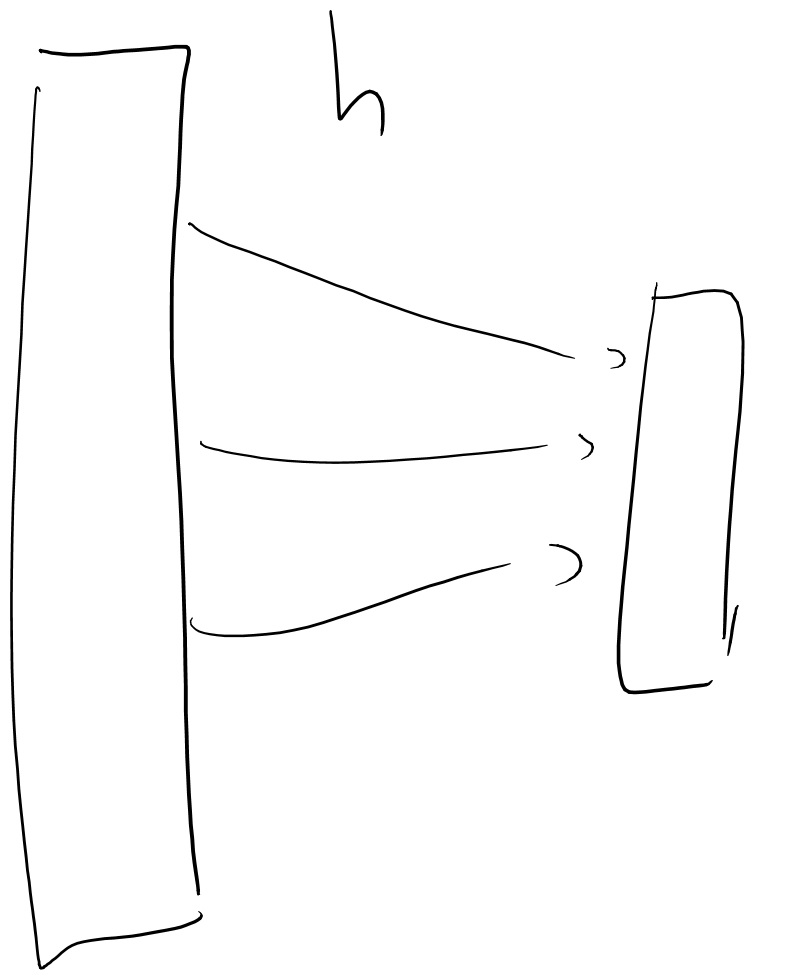
\includegraphics[width=\linewidth, height=1.5in, keepaspectratio]{../figure/hash_function.jpg}
\caption{A collision-resistant hash function is a map that from a large
universe to a small one that is ``practically one to one'' in the sense
that collisions for the function do exist but are hard to find.}
\label{tmplabelfig}
\end{marginfigure}

The main idea is the following simple result, which can be thought of as
one side of the so called \href{https://goo.gl/GSPrDW}{``birthday
paradox''}:

\hypertarget{randomcrhlem}{}
\begin{lemma} \label[lemma]{randomcrhlem}

If \(H\) is a random function from some domain \(S\) to \(\{0,1\}^n\),
then the probability that after \(T\) queries an attacker finds
\(x\neq x'\) such that \(H(x)=H(x')\) is at most \(T^2/2^n\).

\end{lemma}

\begin{proof} \label[proof]{7-Let-us-think-of-H-in-t}

Let us think of \(H\) in the ``lazy evaluation'' mode where for every
query the adversary makes, we choose a random answer in \(\{0,1\}^n\) at
the time it is made. (We can assume the adversary never makes the same
query twice since a repeat query can be simulated by repeating the same
answer.) For \(i< j\) in \([T]\) let \(E_{i,j}\) be the event that
\(H(x_i)=H(x_j)\). Since \(H(x_j)\) is chosen at random and
independently from the prior choice of \(H(x_i)\), the probability of
\(E_{i,j}\) is \(2^{-n}\). Thus the probability of the union of
\(E_{i,j}\) over all \(i,j\)'s is less than \(T^2/2^n\), but this
probability is exactly what we needed to calculate.

\end{proof}

This means that a random function \(H\) is \emph{collision resistant} in
the sense that it is hard for an efficient adversary to find two inputs
that collide. Thus the random oracle heuristic would suggest that a
cryptographic hash function can be used to obtain the following object:

\hypertarget{crhdef}{}
\begin{definition}[Collision resistant hash functions] \label[definition]{crhdef}

A collection \(\{ h_k \}\) of functions where
\(h_k:\{0,1\}^*\rightarrow\{0,1\}^n\) for \(k\in\{0,1\}^n\) is a
\emph{collision resistant hash function (CRH) collection} if the map
\((k,x)\mapsto h_k(x)\) is efficiently computable and for every
efficient adversary \(A\), the probability over \(k\) that
\(A(k)=(x,x')\) such that \(x\neq x'\) and \(h_k(x)=h_k(x')\) is
negligible.\footnote{Note that the other side of the birthday bound
  shows that you can always find a collision in \(h_k\) using roughly
  \(2^{n/2}\) queries. For this reason we typically need to double the
  output length of hash functions compared to the key size of other
  cryptographic primitives (e.g., \(256\) bits as opposed to \(128\)
  bits).}

\end{definition}

Once more we do \emph{not} know a theorem saying that under the PRG
conjecture there exists a collision resistant hash function collection,
even though this property is considered as one of the desiderata for
cryptographic hash functions. However, we do know how to obtain
collections satisfying this condition under various assumptions that we
will see later in the course such as the learning with error problem and
the factoring and discrete logarithm problems. Furthermore if we
consider the weaker notion of security under a \emph{second preimage
attack} (also known as being a ``universal one way hash function'' or
UOWHF) then it \emph{is} known how to derive such a function from the
PRG assumption.

\hypertarget{crhvsprfrem}{}
\begin{remark}[CRH vs PRF] \label[remark]{crhvsprfrem}

A collection \(\{ h_k \}\) of collision resistant hash functions is an
incomparable object to a collection \(\{ f_s \}\) of pseudorandom
functions with the same input and output lengths. On one hand, the
condition of being collision-resistant does not imply that \(h_k\) is
indistinguishable from random. For example, it is possible to construct
a valid collision resistant hash function where the first output bit
always equals zero (and hence is easily distinguishable from a random
function). On the other hand, unlike \cref{prfdef}, the adversary of
\cref{crhdef} is not merely given a ``black box'' to compute the hash
function, but rather the key to the hash function. This is a much
stronger attack model, and so a PRF does not have to be collision
resistant. (Constructing a PRF that is not collision resistant is a nice
and recommended exercise.)

\end{remark}

\section{Practical Constructions of Cryptographic Hash
Functions}\label{7-Practical-Construction}

While we discussed hash functions as \emph{keyed} collections, in
practice people often think of a hash function as being a \emph{fixed
keyless function}. However, this is because most practical constructions
involve some hardwired standardized constants (often known as IV) that
can be thought of as a choice of the key.

Practical constructions of cryptographic hash functions start with a
basic block which is known as a \emph{compression function}
\(h:\{0,1\}^{2n}\rightarrow\{0,1\}^n\). The function
\(H:\{0,1\}^*\rightarrow\{0,1\}^n\) is defined as
\(H(m_1,\ldots,m_t)=h(h(h(m_1,\ensuremath{\mathit{IV}}),m_2),\cdots,m_t)\)
when the message is composed of \(t\) blocks (and we can pad it
otherwise). See \cref{merkledamgardfig}. This construction is known as
the Merkle-Damgard construction and we know that it does preserve
collision resistance:

\begin{figure}
\centering
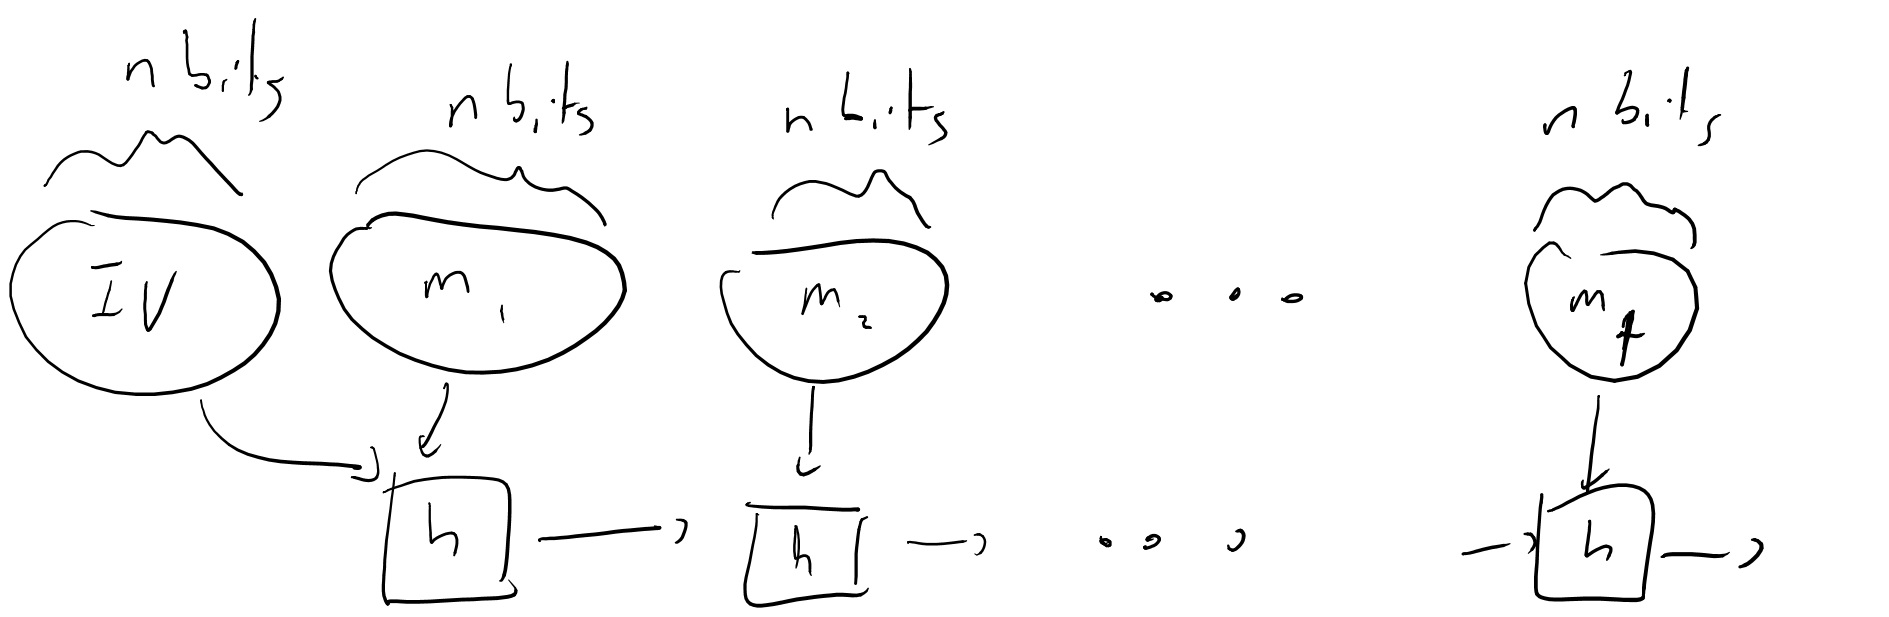
\includegraphics[width=\textwidth, height=0.25\paperheight, keepaspectratio]{../figure/merke-damgard.jpg}
\caption{The Merkle-Damgard construction converts a compression function
\(h:\{0,1\}^{2n}\rightarrow\{0,1\}^n\) into a hash function that maps
strings of arbitrary length into \(\{0,1\}^n\). The transformation
preserves collision resistance but does not yield a PRF even if \(h\)
was pseudorandom. Hence for many applications it should not be used
directly but rather composed with a transformation such as HMAC.}
\label{merkledamgardfig}
\end{figure}

\hypertarget{merkledamgardcrhthm}{}
\begin{theorem}[Merkle-Damgard preserves collision resistance] \label[theorem]{merkledamgardcrhthm}

Let \(H\) be constructed from \(h\) as above. Then given two messages
\(m \neq m' \in \{0,1\}^{tn}\) such that \(H(m)=H(m')\) we can
efficiently find two messages \(x \neq x' \in \{0,1\}^{2n}\) such that
\(h(x)=h(x')\).

\end{theorem}

\begin{proof} \label[proof]{7-The-intuition-behind-t}

The intuition behind the proof is that if \(h\) was invertible then we
could invert \(H\) by simply going backwards. Thus in principle if a
collision for \(H\) exists then so does a collision for \(h\). Now of
course this is a vacuous statement since both \(h\) and \(H\) shrink
their inputs and hence clearly have collisions. But we want to show a
\emph{constructive} proof for this statement that will allow us to
transform a collision in \(H\) to a collision in \(h\). This is very
simple. We look at the computation of \(H(m)\) and \(H(m')\) and at the
first block in which the inputs differ but the output is the same (there
must be such a block). This block will yield a collision for \(h\).

\end{proof}

\subsection{Practical Random-ish
Functions}\label{7-Practical-Random-ish-F}

In practice we want much more than collision resistance from our hash
functions. In particular we often would like them to be PRF's as well.
Unfortunately, the Merkle-Damgard construction is \emph{not} a PRF even
when \(\ensuremath{\mathit{IV}}\) is random and secret. This is because
we can perform a \emph{length extension attack} on it. Even if we don't
know \(\ensuremath{\mathit{IV}}\), given \(y=H_{IV}(m_1,\ldots,m_t)\)
and a block \(m_{t+1}\) we can compute \(y' = h(y,m_{t+1})\) which
equals \(H_{IV}(m_1,\ldots,m_{t+1})\).

One fix for this is to use a different \(\ensuremath{\mathit{IV}}'\) in
the \emph{end} of the encryption. That is, we define:

\(H_{IV,\ensuremath{\mathit{IV}}'}(m_1,\ldots,m_t) = h(\ensuremath{\mathit{IV}}',H_{IV}(m_1,\ldots,m_t))\)

A variant of this construction (where \(\ensuremath{\mathit{IV}}'\) is
obtained as some simple function of \(\ensuremath{\mathit{IV}}\)) is
known as HMAC and it can be shown to be a pseudorandom function under
some pseudorandomness assumptions on the compression function \(h\). It
is very widely implemented. In many cases where I say ``use a
cryptographic hash function'' in this course I actually mean to use an
HMAC like construction that can be conjectured to give at least a PRF if
not stronger ``random oracle''-like properties.

The simplest implementation for a compression function is to take a
\emph{block cipher} with an \(n\) bit key and an \(n\) bit message and
then simply define
\(h(x_1,\ldots,x_{2n})=E_{x_{n+1},\ldots,x_{2n}}(x_{1},\ldots,x_{n})\).
A more common variant is known as Davies-Meyer where we also XOR the
output with \(x_{n+1},\ldots x_{2n}\). In practice people often use
\emph{tailor made} block ciphers that are designed for some efficiency
or security concerns.

\subsection{Some History}\label{7-Some-History}

Almost all practically used hash functions are based on the
Merkle-Damgard paradigm. Hash functions are designed to be extremely
efficient\footnote{For example, the Boneh-Shoup book quotes processing
  times of up to 255MB/sec on a 1.83 Ghz Intel Core 2 processor, which
  is more than enough to handle not just Harvard's network but even
  \href{http://www.huffingtonpost.com/2014/06/27/colleges-fastest-internet-speed-infographic_n_5536834.html}{Lamar
  College's}.} which also means that they are often at the ``edge of
insecurity'' and indeed have fallen over the edge.

In 1990 Ron Rivest proposed MD4, which was already showing weaknesses in
1991, and a full collision was found in 1995. Even faster attacks have
been since found and MD4 is considered completely insecure.

In response to these weaknesses, Rivest designed MD5 in 1991. A weakness
was shown for it in 1996 and a full collision was shown in 2004. Hence
it is now also considered insecure.

In 1993 the National Institute of Standards proposed a standard for a
hash function known as the \emph{Secure Hash Algorithm (SHA)}, which had
quite a few similarities with the MD4 and MD5 functions. This function
was known as SHA-0, and the standard was replaced in 1995 with SHA-1,
which includes an extra ``mixing'' (i.e., bit rotation) operation. At
the time no explanation was given for this change, but SHA-0 was later
found to be insecure. In 2002 a variant with longer output, known as
SHA-256, was added (as well as some others). In 2005, following the MD5
collision, significant weaknesses were shown in SHA-1. In 2017, a
\href{https://goo.gl/jdqUX9}{full SHA-1 collision was found}. Today
SHA-1 is considered insecure and SHA-256 is recommended.

Given the weaknesses in MD-5 and SHA-1, NIST started a competition in
2006 for a new hashing standard, based on functions that seem
sufficiently different from the MD5/SHA-0/SHA-1 family. (SHA-256 is
unbroken but it seems too close for comfort to those other systems.) The
hash function Keccak was selected as the new standard
\href{https://goo.gl/Bx1bu2}{SHA-3} in August of 2015.

\subsection{The NSA and Hash Functions}\label{7-The-NSA-and-Hash-Funct}

The NSA is the world's largest employer of mathematicians, and is very
heavily invested in cryptographic research. It seems quite possible that
they devote far more resources to analyzing symmetric primitives such as
block ciphers and hash functions than the open research community.
Indeed, the history above suggests that the NSA has consistently
discovered attacks on hash functions before the cryptographic community
(and the same holds for the differential cryptanalysis technique for
block ciphers). That said, despite the ``mythic'' powers that are
sometimes ascribed to the NSA, this history suggests that they are ahead
of the open community, but not so much ahead, discovering attacks on
hash functions about 5 years or so before they appear in the open
literature.

There are a few ways we can get ``insider views'' to the NSA's thinking.
Some such insights can be obtained from the Snowden documents. The
\href{https://en.wikipedia.org/wiki/Flame_(malware)}{Flame malware} was
discovered in Iran in 2012 after operating since at least 2010. It used
an MD5 collision to achieve its goals. Such a collision was known in the
open literature since 2008, but Flame used a different variant that was
unknown in the literature. For this reason it is suspected that it was
designed by a western intelligence agency.

Another insight into NSA's thoughts can be found in pages 12-19 of NSA's
internal
\href{https://cryptome.org/2013/03/cryptologs/cryptolog_126.pdf}{Cryptolog
newsletter} which was recently declassified; one can find there a rather
entertaining and opinionated (or obnoxious, depending on your point of
view) review of the CRYPTO 1992 conference. In page 14 the author
remarks that certain weaknesses of MD5 demonstrated in the conference
are unlikely to be extended to the full version, which suggests that the
NSA (or at least the author) was not aware of the MD5 collisions at the
time. (The
\href{https://cryptome.org/2013/03/cryptologs/00-cryptolog-index.htm}{full
archive} of the cryptolog newsletter makes for some interesting
reading!)

\subsection{Cryptographic vs Non-Cryptographic Hash
Functions}\label{7-Cryptographic-vs-Non-C}

Hash functions are of course also widely used for
\emph{non-cryptographic} applications such as building hash tables and
load balancing. For these applications people often use \emph{linear}
hash functions known as \emph{cyclic redundancy codes (CRC)}. Note
however that even in those seemingly non-cryptographic applications, an
adversary might cause significant slowdown to the system if he can
generate many collisions. This can and
\href{http://arstechnica.com/business/2011/12/huge-portions-of-web-vulnerable-to-hashing-denial-of-service-attack/}{has}
been used to obtain denial of service attacks. As a rule of thumb, if
the inputs to your system might be generated by someone who does not
have your best interests at heart, you're better off using a
cryptographic hash function.

\section{Reading comprehension
exercises}\label{7-Reading-comprehension-}

I recommend students do the following exercises after reading the
lecture. They do not cover all material, but can be a good way to check
your understanding.

\begin{exercise} \label[exercise]{7-Choose-the-strongest-t}

Choose the strongest true statement from the following options. (That
is, choose the mathematical statement from these options that is both
true, and one can derive the other true statements as direct
corollaries.)

\begin{enumerate}
\def\labelenumi{\alph{enumi}.}
\item
  For every function \(h:\{0,1\}^{1024} \rightarrow \{0,1\}^{128}\)
  there exist two strings \(x \neq x'\) in \(\{0,1\}^{1024}\) such that
  \(h(x)=h(x')\).
\item
  There is a randomized algorithm \(A\) that makes at most \(2^{128}\)
  queries to a given black box computing a function
  \(h:\{0,1\}^{1024} \rightarrow \{0,1\}^{128}\) that with probability
  at least \(0.9\), \(A\) outputs a pair \(x \neq x'\) in
  \(\{0,1\}^{1024}\) such that \(h(x)=h(x')\).
\item
  There is a randomized algorithm \(A\) that makes at most
  \(100 \cdot 2^{64}\) queries to a given black box computing a function
  \(h:\{0,1\}^{1024} \rightarrow \{0,1\}^{128}\) that with probability
  at least \(0.9\), \(A\) outputs a pair \(x \neq x'\) in
  \(\{0,1\}^{1024}\) such that \(h(x)=h(x')\).
\item
  There is a randomized algorithm \(A\) that makes at most
  \(0.01 \cdot 2^{64}\) queries to a given black box computing a
  function \(h:\{0,1\}^{1024} \rightarrow \{0,1\}^{128}\) that with
  probability at least \(0.9\), \(A\) outputs a pair \(x \neq x'\) in
  \(\{0,1\}^{1024}\) such that \(h(x)=h(x')\).
\end{enumerate}

\end{exercise}

\begin{exercise} \label[exercise]{7-Suppose-that-h-rightar}

Suppose that \(h:\{0,1\}^{1024} \rightarrow \{0,1\}^{128}\) is chosen at
random. If \(y\) is chosen at random in \(\{0,1\}^{128}\) and we pick
\(x_1,\ldots,x_t\) independently at random in \(\{0,1\}^{1024}\), how
large does \(t\) need to be so that the probability that there is some
\(x_i\) such that \(h(x_i)=y\) is at least \(1/2\). (Pick the answer
with the closest estimate):

\begin{enumerate}
\def\labelenumi{\alph{enumi}.}
\item
  \(2^{1024}\)
\item
  \(2^{256}\)
\item
  \(2^{128}\)
\item
  \(2^{64}\)
\end{enumerate}

\end{exercise}

\begin{exercise} \label[exercise]{7-Suppose-that-a-message}

Suppose that a message authentication code \((S,V)\) where Alice and Bob
use as one of its components a function \(h\) as a black box is secure
when \(h\) is a random function. Is it still secure when Alice and Bob
uses a hash function \(h\) that is chosen from some PRF collection and
whose key is given to the adversary?

\begin{enumerate}
\def\labelenumi{\alph{enumi}.}
\item
  It can sometimes be secure and sometimes insecure.
\item
  It is always secure.
\item
  It is always insecure.
\end{enumerate}

\end{exercise}

\chapter{Key derivation, protecting passwords, slow hashes, Merkle
trees}\label{Key-derivation-protecting-pass}

Last lecture we saw the notion of cryptographic hash functions which are
functions that behave like a random function, even in settings (unlike
that of standard PRFs) where the adversary has access to the key that
allows them to evaluate the hash function. Hash functions have found a
variety of uses in cryptography, and in this lecture we survey some of
their other applications. In some of these cases, we only need the
relatively mild and well-defined property of \emph{collision resistance}
while in others we only know how to analyze security under the stronger
(and not precisely well defined) \emph{random oracle heuristic}.

\section{Keys from passwords}\label{Keys-from-passwords}

We have seen great cryptographic tools, including PRFs, MACs, and CCA
secure encryptions, that Alice and Bob can use when they share a
cryptographic key of 128 bits or so. But unfortunately, many of the
current users of cryptography are \emph{humans} which, generally
speaking, have extremely faulty memory capacity for storing large
numbers. There are \(62^8 \approx 2^{48}\) ways to select a password of
8 upper and lower case letters + numbers, but some letter/numbers
combinations end up being chosen much more frequently than others. Due
to several large scale hacks, very large databases of passwords have
been made public, and one
\href{https://blogs.dropbox.com/tech/2012/04/zxcvbn-realistic-password-strength-estimation/}{estimate}
is that 91 percent of the passwords chosen by users are contained in a
list of about \(1,000 \approx 2^{10}\) strings.

If we choose a password at random from some set \(D\) then the
\emph{entropy} of the password is simply \(\log_2 |D|\). However,
estimating the entropy of real life passwords is rather difficult. For
example, suppose that I use the winning Massachussets Mega-Lottery
numbers as my password. A priori, my password consists of \(5\) numbers
between \(1\) till \(75\) and so its entropy is
\(\log_2 (75^5) \approx 31\). However, if an attacker \emph{knew} that I
did this, the entropy might be something like \(\log(520) \approx 9\)
(since there were only 520 such numbers selected in the last 10 years).
Moreover, if they knew exactly what draw I based my password on, then
they would it exactly and hence the entropy (from their point of view)
would be zero. This is worthwhile to emphasize:

\begin{quote}
\emph{The entropy of a secret is always measured with respect to the
attacker's point of view.}
\end{quote}

The exact security of passwords is of course a matter of intense
practical interest, but we will simply model the password as being
chosen at random from some set \(D\subseteq\{0,1\}^n\) (which is
sometimes called the ``dictionary''). The set \(D\) is known to the
attacker, but she has no information on the particular choice of the
password.

Much of the challenge for using passwords securely relies on the
distinction between \emph{offline} and \emph{online} attacks. If each
guess for a password requires interacting \emph{online} with a server,
as is the case when typing a PIN number in the ATM, then even a weak
password (such as a 4 digit PIN that at best provides \(13\) bits of
entropy) can yield meaningful security guarantees, as typically an alarm
would be raised after five or so failed attempts.\\
However, if the adversary has the ability to check \emph{offline}
whether a password is correct then the number of guesses they can try
can be as high as the number of computing cycles at their disposal,
which can easily run into the billions and so break passwords of \(30\)
or more bits of entropy. (This is an issue we'll return to after we
learn about \emph{public key cryptography} when we'll talk about
\emph{password authenticated key exchange}.)

Consider a password manager application. In such an application, a user
typically chooses a \emph{master password} \(p_{master}\) which she can
then use to access all her other passwords \(p_1,\ldots,p_t\). To enable
her to do so without requiring online access to a server, the master
password \(p_{master}\) is used to \emph{encrypt} the other passwords.
However to do that, we need to derive a key \(k_{master}\) from the
password.

\begin{pause} \label[pause]{A-natural-approach-is-to-simpl}

A natural approach is to simply let the key be the password. For
example, if the password \(p\) is a string of at most 16 bytes, then we
can simply treat it as a \(128\) bit key and use it for encryption. Stop
and think why this would \emph{not} be a good idea. In particular think
of an example of a secure encryption \((E,D)\) and a distribution \(P\)
over \(\{0,1\}^n\) of entropy at least \(n/2\) such that if the key
\(k\) is chosen at random from \(P\) then the encryption will be
completely insecure.

\end{pause}

A classical approach is to simply use a cryptographic hash function
\(H:\{0,1\}^*\rightarrow\{0,1\}^n\), and let
\(k_{master} = H(p_{master})\). If think of \(H\) as a random oracle and
\(p_{master}\) as chosen randomly from \(D\), then as long as an
attacker makes \(\ll |D|\) queries to the oracle, they are unlikely to
make the query \(p_{master}\) and hence the value \(k_{master}\) will be
completely random from their point of view.

However, since \(|D|\) is not too large, it might not be so hard to
perform such \(|D|\) queries. For this reason, people typically use a
\emph{deliberately slow hash} function as a \emph{key derivation
function}. The rationale is that the honest user only needs to evaluate
\(H\) once, and so could afford for it to take a while, while the
adversary would need to evaluate it \(|D|\) times. For example, if
\(|D|\) is about \(100,000\) and the honest user is willing to spend 1
cent of computation resources every time they need to derive
\(k_{master}\) from \(p_{master}\), then we could set \(H(\cdot)\) so
that it costs 1 cent to evaluate it and hence on average it will cost
the adversary \(1,000\) dollars to recover it.

There are several approaches for trying to make \(H\) deliberately
``slow'' or ``costly'' to evaluate but the most popular and simplest one
is to simply let \(H\) be obtained by iterating many times a basic hash
function such as SHA-256. That is, \(H(x)=h(h(h(\cdots h(x))))\) where
\(h\) is some standard (``fast'') cryptographic hash function and the
number of iterations is tailored to be the largest one that the honest
users can tolerate.\footnote{Since CPU speeds can vary quite radically
  and attackers might even use special-purpose hardware to evaluate
  iterated hash functions quickly, Abadi, Burrows, Manasse, and Wobber
  suggested in 2003 to use \emph{memory bound} functions as an
  alternative approach, where these are functions \(H(\cdot)\) designed
  so that evaluating them will consume at least \(T\) bits of memory for
  some large \(T\). See also the followup paper of Dwork, Goldberg and
  Naor. This approach has also been used in some practical key
  derivation functions such as \texttt{scrypt} and
  \href{https://password-hashing.net/argon2-specs.pdf}{\texttt{Argon2}}.}

In fact, typically we will set \(k_{master} = H(p_{master}\| r)\) where
\(r\) is a long random but \emph{public} string known as a ``salt'' (see
\cref{saltfig}). Including such a ``salt'' can be important to foiling
an adversary's attempts to amortize the computation costs, see the
exercises.

\begin{figure}
\centering
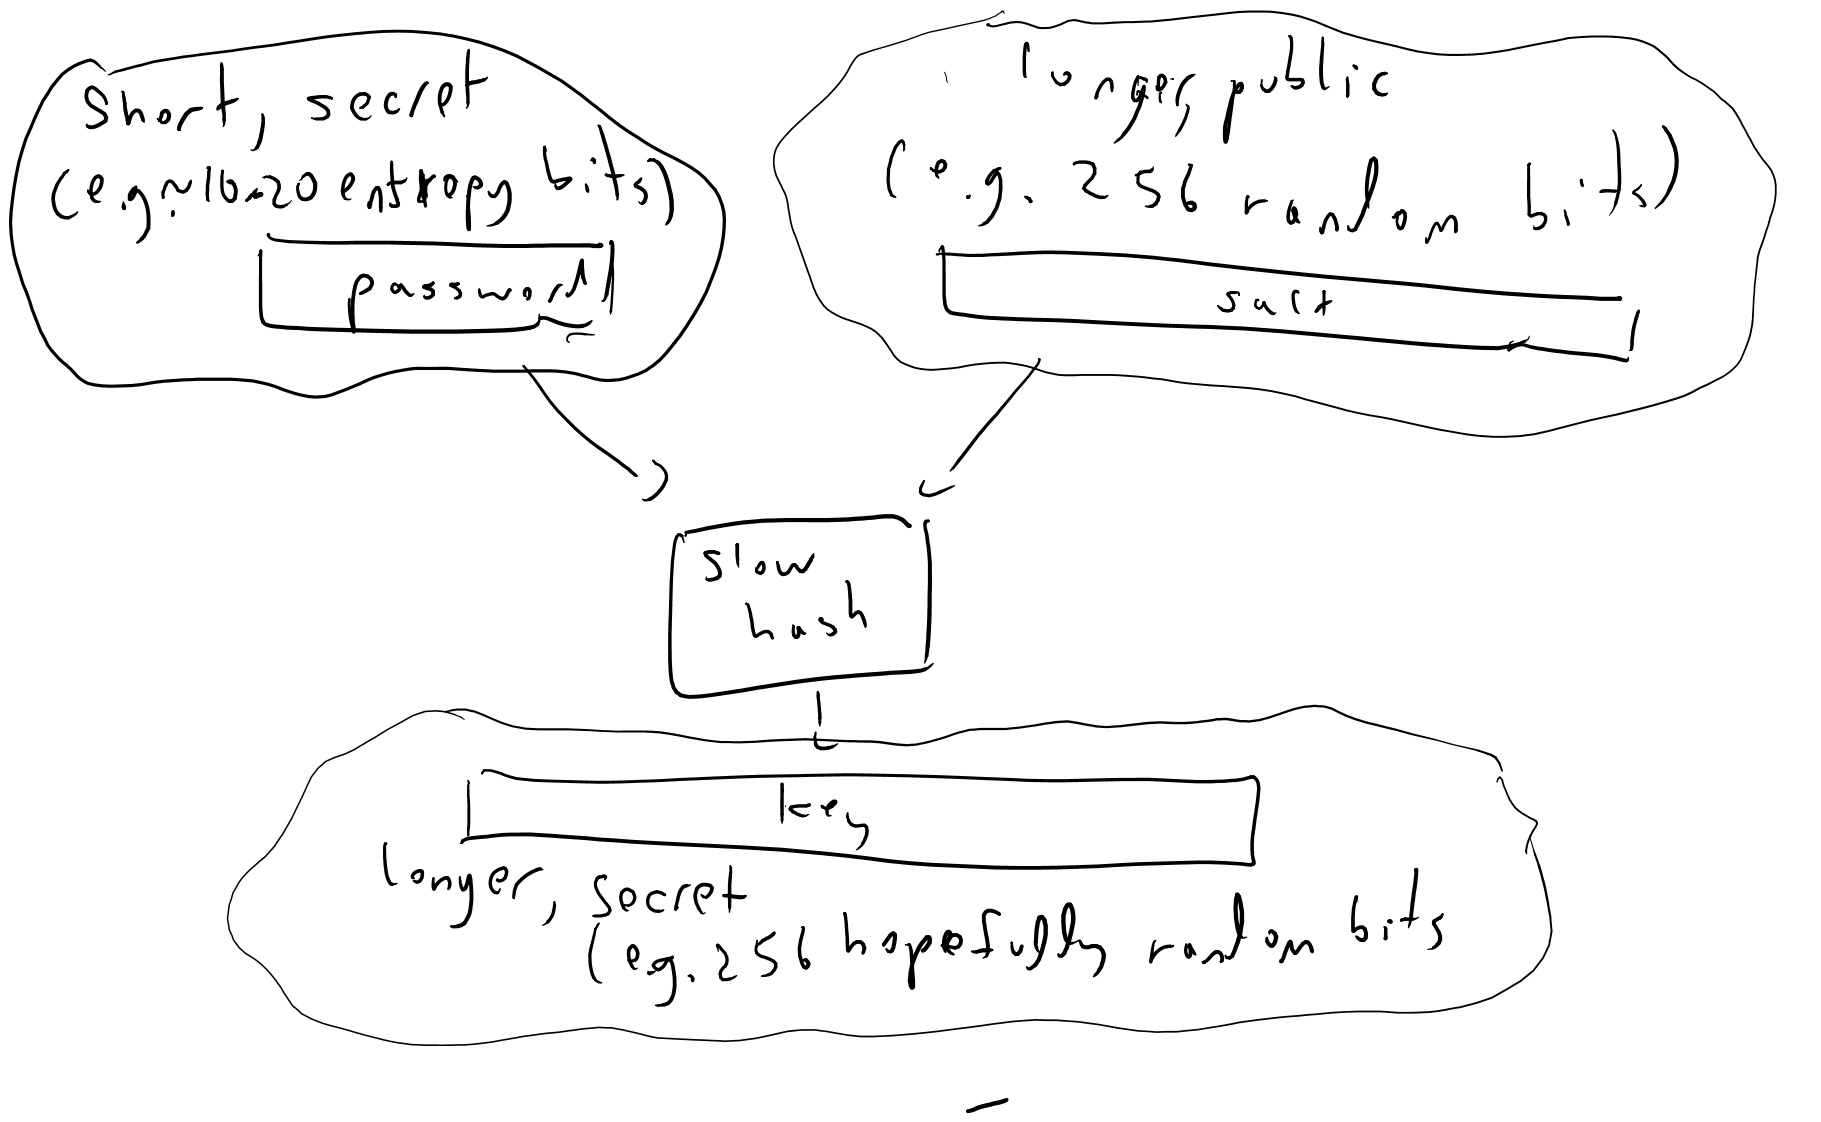
\includegraphics[width=\textwidth, height=0.25\paperheight, keepaspectratio]{../figure/hash-password.jpg}
\caption{To obtain a key from a password we will typically use a
``slow'' hash function to map the password and a unique-to-user public
``salt'' value to a cryptographic key. Even with such a procedure, the
resulting key cannot be consider as secure and unpredictable as a key
that was chosen truly at random, especially if we are in a setting where
an adversary can launch an \emph{offline} attack to guess all
possibilities.}
\label{saltfig}
\end{figure}

Even when we don't use one password to encrypt others, it is generally
considered the best practice to \emph{never} store a password in the
clear but always in this ``slow hashed and salted'' form, so if the
passwords file falls to the hands of an adversary it will be expensive
to recover them.

\section{Merkle trees and verifying
storage.}\label{Merkle-trees-and-verifying-sto}

Suppose that you outsource to the cloud storing your huge data file
\(x\in\{0,1\}^N\). You now need the \(i^{th}\) bit of that file and ask
the cloud for \(x_i\). How can you tell that you actually received the
correct bit?

Ralph Merkle came up in 1979 with a clever solution, which is known as
``Merkle hash trees''. The idea is the following (see
\cref{merkletreefig}): suppose we have a collision-resistant hash
function \(h:\{0,1\}^{2n}\rightarrow\{0,1\}^n\), and think of the string
\(x\) as composed of \(t\) blocks of size \(n\). We then hash every pair
of consecutive blocks to transform \(x\) into a string \(x_1\) of
\(t/2\) blocks, and continue in this way for \(\log t\) steps until we
get a single block \(y\in\{0,1\}^n\). (Assume here \(t\) is a power of
two for simplicity, though it doesn't make much difference.)

\begin{figure}
\centering
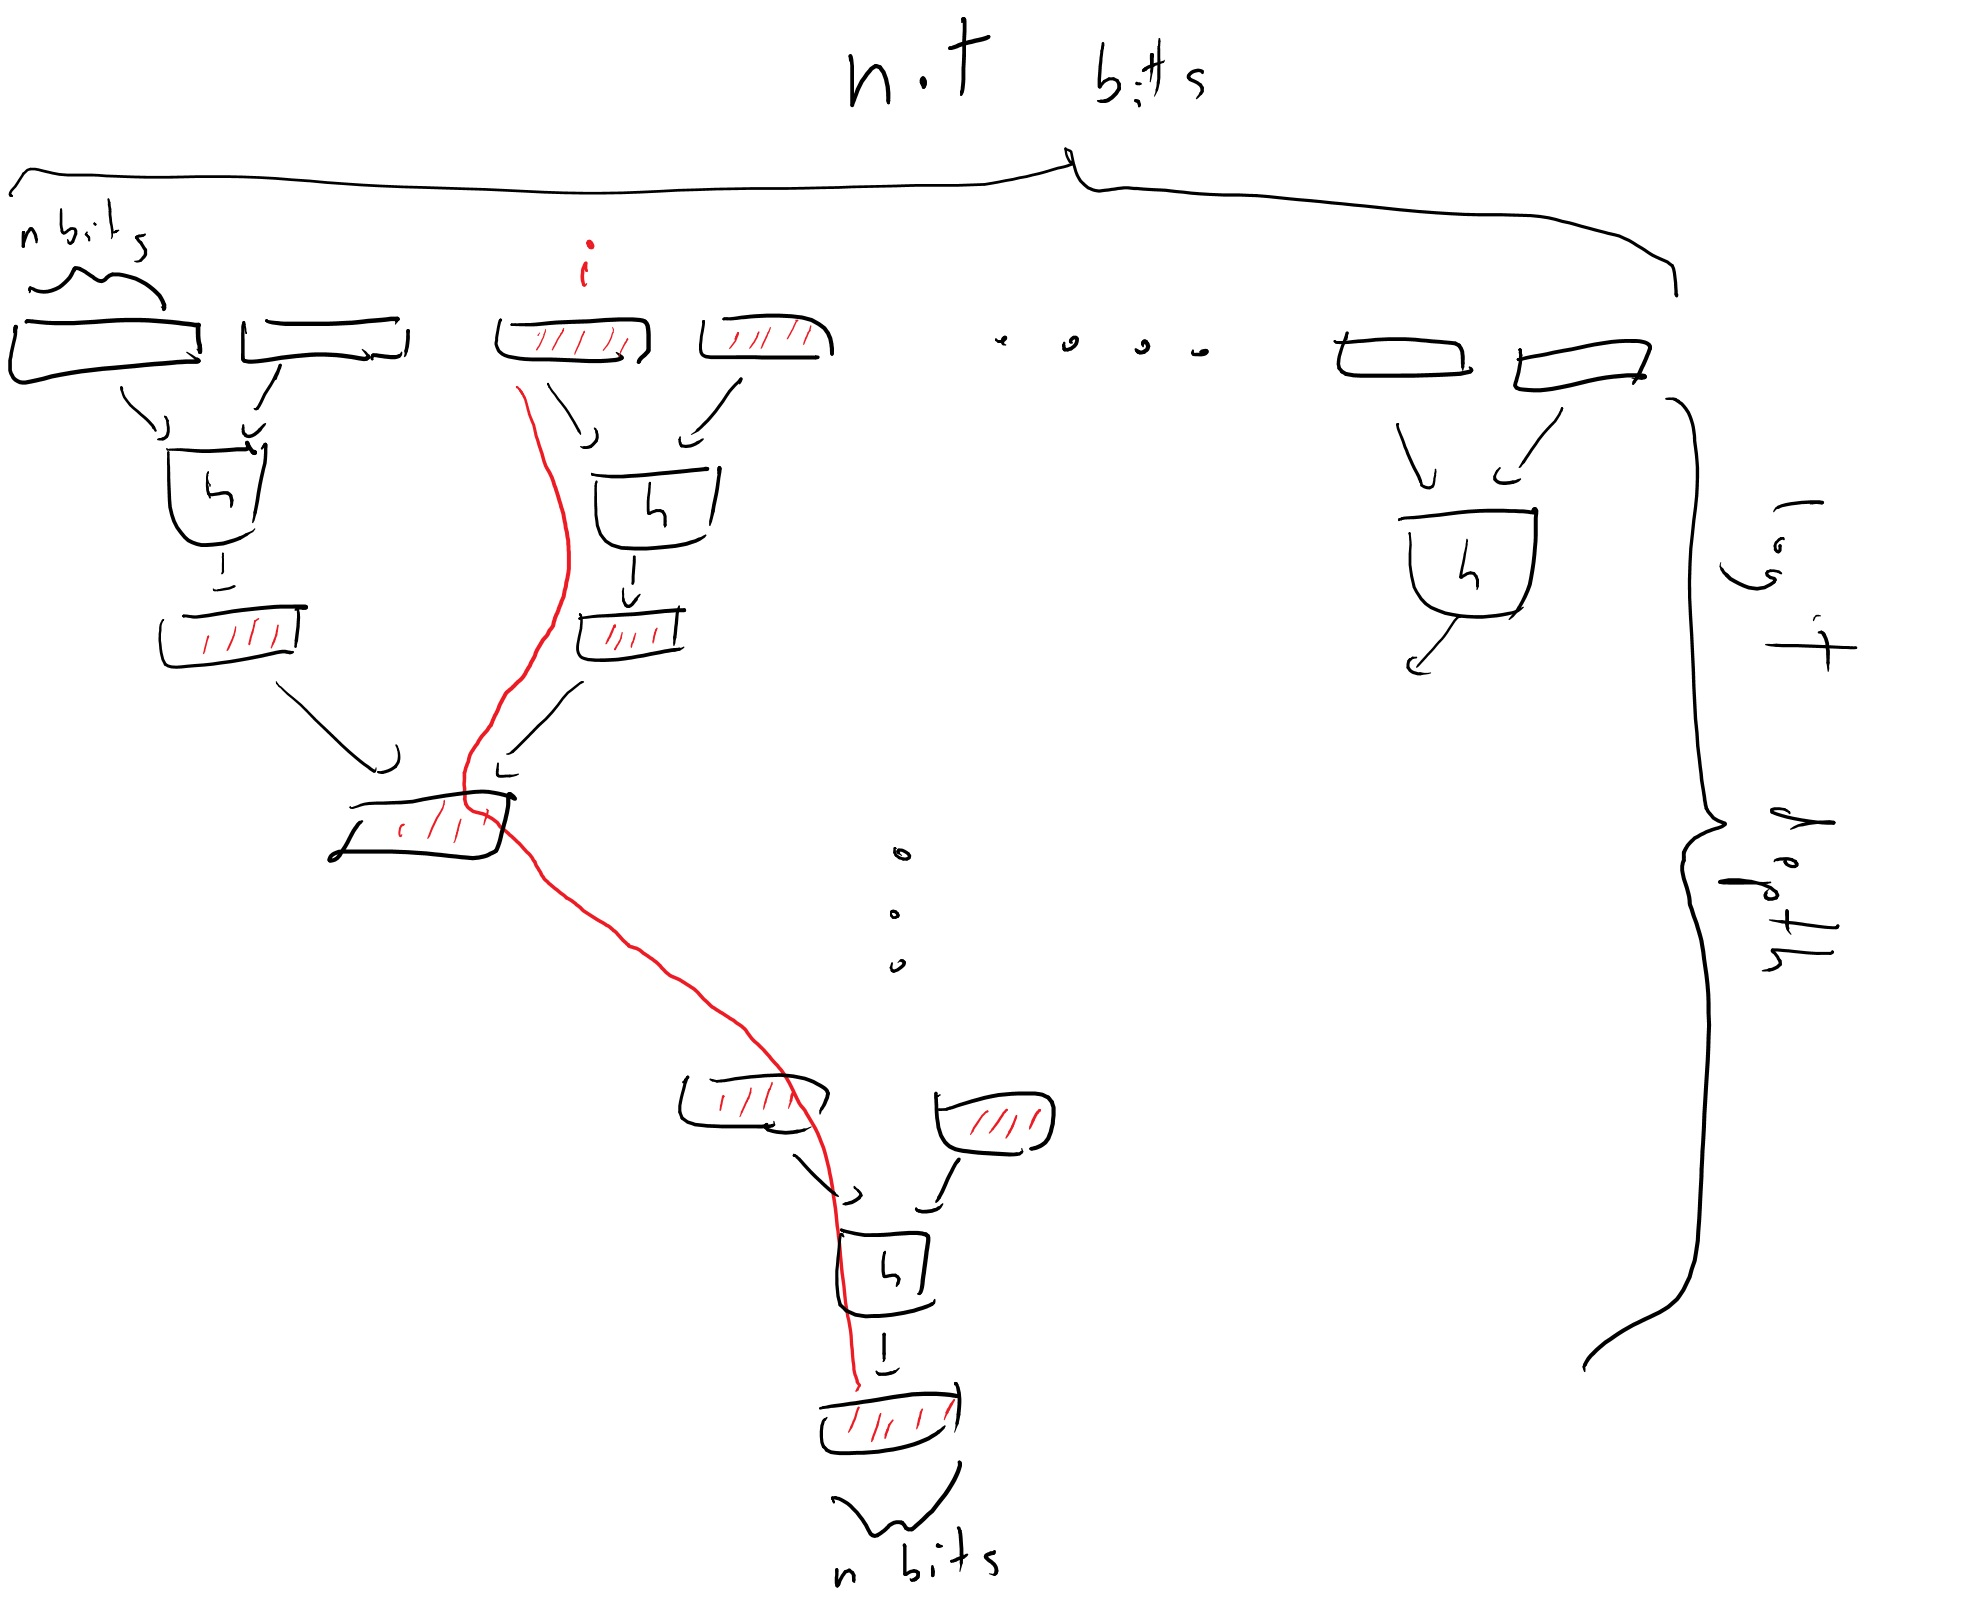
\includegraphics[width=\textwidth, height=0.25\paperheight, keepaspectratio]{../figure/merkle-tree.jpg}
\caption{In the Merkle Tree construction we map a long string \(x\) into
a block \(y\in\{0,1\}^n\) that is a ``digest'' of the long string \(x\).
As in a collision resistant hash we can imagine that this map is ``one
to one'' in the sense that it won't be possible to find \(x'\neq x\)
with the same digest. Moreover, we can efficiently certify that a
certain bit of \(x\) is equal to some value without sending out all of
\(x\) but rather the \(\log t\) blocks that are on the path between
\(i\) to the root together with their ``siblings'' used in the hash
function, for a total of at most \(2\log t\) blocks.}
\label{merkletreefig}
\end{figure}

Alice who sends \(x\) to the cloud Bob will keep the short block \(y\).
Whenever Alice queries the value \(i\) she will ask for a
\emph{certificate} that \(x_i\) is indeed the right value. This
certificate will consists of the block that contains \(i\), as well as
all of the \(2\log t\) blocks that were used in the hash from this block
to the root. The security of this scheme follows from the following
simple theorem:

\hypertarget{merkletreefig}{}
\begin{theorem}[Merkle Tree security] \label[theorem]{merkletreefig}

Suppose that \(\pi\) is a valid certificate that \(x_i=b\), then either
this statement is true, or one can efficiently extract from \(\pi\) and
\(x\) two inputs \(z\neq z'\) in \(\{0,1\}^{2n}\) such that
\(h(z)=h(z')\).

\end{theorem}

\begin{proof} \label[proof]{The-certificate-pi-consists-of}

The certificate \(\pi\) consists of a sequence of \(\log t\) pairs of
size-\(n\) blocks that are obtained by following the path on the tree
from the \(i^{th}\) coordinate of \(x\) to the final root \(y\). The
last pair of blocks is the a preimage of \(y\) under \(h\), while each
pair on this list is a preimage of one of the blocks in the next pair.
If \(x_i \neq b\), then the first pair of blocks cannot be identical to
the pair of blocks of \(x\) that contains the \(i^{th}\) coordinate.
However, since we know the final root \(y\) is identical, if we compare
the corresponding path in \(x\) to \(\pi\), we will see that at some
point there must be an input \(z\) in the path from \(x\) and a distinct
input \(z'\) in \(\pi\) that hash to the same output.

\end{proof}

\section{Proofs of Retrievability}\label{Proofs-of-Retrievability}

The above provides a way to ensure Alice that the value retrieved from a
cloud storage is correct, but how can Alice be sure that the cloud
server still stores the values that she \emph{did not} ask about?

A priori, you might think that she obviously can't. If Bob is lazy, or
short on storage, he could decide to store only some small fraction of
\(x\) that he thinks Alice is more likely to query for. As long as Bob
wasn't unlucky and Alice doesn't ask these queries, then it seems Bob
could get away with this. In a \emph{proof of retrievability}, first
proposed by Juels and Kalisky in 2007, Alice would be able to get
convinced that Bob does in fact store her data.

First, note that Alice can guarantee that Bob stores at least 99 percent
of her data, by periodically asking him to provide answers (with
proofs!) of the value of \(x\) at 100 or so random locations. The idea
is that if bob dropped more than 1 percent of the bits, then he'd be
very likely to be caught ``red handed'' and get a question from Alice
about a location he did not retain.

Now, if we used some redundancy to store \(x\) such as the RAID format,
where it is composed of some small number \(c\) parts and we can recover
any bit of the original data as long as at most one of the parts were
lost, then we might hope that even if 1\% of \(x\) \emph{was} in fact
lost by Bob, we could still recover the whole string. This is not a
fool-proof guarantee since it could possibly be that the data lost by
Bob was not confined to a single part. To handle this case one needs to
consider generalizations of RAID known as ``local reconstruction codes''
or ``locally decodable codes''. The paper by
\href{http://www.people.seas.harvard.edu/~salil/research/PoR-tcc09.pdf}{Dodis,
Vadhan and Wichs} is a good source for this; see also
\href{http://research.microsoft.com/en-us/um/people/senyk/slides/pos-cai.pdf}{these
slides by Seny Kamara} for a more recent overview of the theory and
implementations.

\section{Entropy extraction}\label{Entropy-extraction}

As we've seen time and again, \emph{randomness} is crucial to
cryptography. But how \emph{do} we get these random bits we need? If we
only have a small number \(n\) of random bits (e.g., \(n=128\) or so)
then we can expand them to as large a number as we want using a
pseudorandom generator, but where do we get those initial \(n\) bits
from?

The approach used in practice is known as ``harvesting entropy''. The
idea is that we make great many measurements \(x_1,\ldots,x_m\) of
events that are considered ``unpredictable'' to some extent, including
mouse movements, hard-disk and network latency, sources of noise
etc\ldots{} and accumulate them in an entropy ``pool'' which would
simply be some memory array. When we estimate that we have accumulated
more than \(128\) bits of randomness, then we hash this array into a
\(128\) bit string which we'll use as a seed for a pseudorandom
generator (see \cref{entropyextfig}).\footnote{The reason that people
  use entropy ``pools'' rather than simply adding the entropy to the
  generator's state as it comes along is that the latter alternative
  might be insecure. Suppose that initial state of the generator was
  known to the adversary and now the entropy is ``trickling in'' one bit
  at a time while we continuously use the generator to produce outputs
  that can be observed by the adversary. Every time a new bit of entropy
  is added, the adversary now has uncertainty between two potential
  states of the generator, but once an output is produced this
  eliminates this uncertainty. In contrast, if we wait until we
  accumulate, say, 128 bits of entropy, then now the adversary will have
  \(2^{128}\) possible state options to consider, and it could be
  computationally infeasible to cull them using further observation.}
Because entropy needs to be measured \emph{from the point of view of the
attacker}, this ``entropy estimation'' routine is a bit of a ``black
art'' and there isn't a very principled way to perform it. In practice
people try to be very conservative (e.g., assume that there is only one
bit of entropy for 64 bits of measurements or so) and hope for the best,
which often works but sometimes also
\href{https://factorable.net/paper.html}{spectacularly fails},
especially in embedded systems that do not have access to many of these
sources.

\begin{figure}
\centering
\includegraphics[width=\textwidth, height=0.25\paperheight, keepaspectratio]{../figure/extraction.jpg}
\caption{To obtain pseudorandom bits for cryptographic applications we
hash down measurements which contain some \emph{entropy} in them to a
shorter string that is hopefully truly uniformly random or at least
statistically close to it, and then expand this to get as many
pseudorandom bits as we need using a pseudorandom generator.}
\label{entropyextfig}
\end{figure}

How do hash functions figure into this? The idea is that if an input
\(x\) has \(n\) bits of entropy then \(h(x)\) would still have the same
bits of entropy, as long as its output is larger than \(n\). In practice
people use the notion of ``entropy'' in a rather loose sense, but we
will try to be more precise below.

The \emph{entropy} of a distribution \(D\) is meant to capture the
amount of ``uncertainty'' you have over the distribution. The canonical
example is when \(D\) is the uniform distribution over \(\{0,1\}^n\), in
which case it has \(n\) bits of entropy. If you learn a single bit of
\(D\) then you reduce the entropy by one bit. For example, if you learn
that the \(17^{th}\) bit is equal to \(0\), then the new conditional
distribution \(D'\) is the uniform distribution over all strings in
\(x\in\{0,1\}^n\) such that \(x_{17}=0\) and has \(n-1\) bits of
entropy. Entropy is invariant under permutations of the sample space,
and only depends on the vector of probabilities, and thus for every set
\(S\) all notions of entropy will give \(\log_2 |S|\) bits of entropy
for the uniform distribution over \(S\). A distribution that is uniform
over some set \(S\) is known as a \emph{flat} distribution.

Where different notions of entropy begin to differ is when the
distributions are not flat. The \emph{Shannon entropy} follows the
principle that ``original uncertainty = knowledge learned + new
uncertainty''. That is, it obeys the \emph{chain rule} which is that if
a random variable \((X,Y)\) has \(n\) bits of entropy, and \(X\) has
\(k\) bits of entropy, then after learning \(X\) on average \(Y\) will
have \(n-k\) bits of entropy. That is,

\(H_{Shannon}(X)+H_{Shannon}(Y|X) = H_{Shannon}(X,Y)\)

Where the entropy of a conditional distribution \(Y|X\) is simply
\(\E_{x\leftarrow X} H_{Shannon}(Y|X=x)\) where \(Y|X=x\) is the
distribution on \(Y\) obtained by conditioning on the event that
\(X=x\).

If \((p_1,\ldots,p_m)\) is a vector of probabilities summing up to \(1\)
and let us assume they are rounded so that for every \(i\),
\(p_i = k_i/2^n\) for some integer \(k_i\). We can then split the set
\(\{0,1\}^n\) into \(m\) disjoint sets \(S_1,\ldots,S_m\) where
\(|S_i|=k_i\), and consider the probability distribution \((X,Y)\) where
\(Y\) is uniform over \(\{0,1\}^n\), and \(X\) is equal to \(i\)
whenever \(Y\in S_i\). Therefore, by the principles above we know that
\(H_{Shannon}(X,Y)=n\) (since \(X\) is completely determined \(Y\) and
hence \((X,Y)\) is uniform over a set of \(2^n\) elements), and
\(H(Y|X)= \E \log k_i\). Thus the chain rule tells us that
\(H_{Shannon}(X) = n - \E[Y|X] = n - \sum_{i=1}^m p_i k_i = n - \sum_{i=1}^m p_i \log(2^n p_i)\)
since \(p_i = k_i/2^n\). Since \(\log(2^n p_i) = n + \log(p_i)\) we see
that this means that \[
H_{Shannon}(X) =  n - \sum_i p_i \cdot n  - \sum_i p_i \log(p_i) = - \sum_i p_i \log (p_i)
\] using the fact that \(\sum_i p_i = 1\).

The Shannon entropy has many attractive properties, but it turns out
that for cryptographic applications, the notion of \emph{min entropy} is
more appropriate. For a distribution \(X\) the \emph{min-entropy} is
simply defined as \(H_{\infty}(X)= \min_x \log(1/\Pr[X=x])\).\footnote{The
  notation \(H_{\infty}(\cdot)\) for min entropy comes from the fact
  that one can define a \href{https://goo.gl/HvVgu1}{\emph{family}} of
  entropy like functions, containing a function for every non-negative
  number \(p\) based on the \(p\)-norm of the probability distribution.
  That is, the Rényi entropy of order \(p\) is defined as
  \(H_p(X)=(1-p)^{-1}-\log(\sum_x \Pr[X=x]^p)\). The min entropy can be
  thought of as the limit of \(H_p\) when \(p\) tends to infinity while
  the Shannon entropy is the limit as \(p\) tends to \(1\). The entropy
  \(H_2(\cdot)\) is related to the \emph{collision probability} of \(X\)
  and is often used as well. The min entropy is the smallest among all
  the entropies and hence it is the most \emph{conservative} (and so
  appropriate for usage in cryptography). For \emph{flat sources}, which
  are uniform over a certain subset, all entropies coincide.} Note that
if \(X\) is flat then \(H_{\infty}(X)=H_{Shannon}(X)\) and that
\(H_{\infty}(X) \leq H_{Shannon}(X)\) for all \(X\). We can now formally
define the notion of an extractor:

\hypertarget{extractordef}{}
\begin{definition}[Randomness extractor] \label[definition]{extractordef}

A function \(h:\{0,1\}^{\ell+n}\rightarrow\{0,1\}^n\) is a
\emph{randomness extractor} (``extractor'' for short) if for every
distribution \(X\) over \(\{0,1\}^\ell\) with min entropy at least
\(2n\), if we pick \(s\) to be a random ``salt'', the distribution
\(h(X)\) is computationally indistinguishable from the uniform
distribution.\footnote{The pseudorandomness literature studies the
  notion of extractors much more generally and consider all possible
  variations for parameters such as the entropy requirement, the salt
  (more commonly known as seed) size, the distance from uniformity, and
  more. The type of notion we consider here is known in that literature
  as a ``strong seeded extractor''. See
  \href{https://goo.gl/XHQjTB}{Vadhan's monograph} for an in-depth
  treatment of this topic.}

\end{definition}

The idea is that we apply the hash function to our measurements in
\(\{0,1\}^\ell\) then if those measurements had at least \(k\) bits of
entropy (with some extra ``security margin'') then the output \(h(X)\)
will be as good as random. Since the ``salt'' value \(s\) is not secret,
it can be chosen once at random and hardwired into the description of
the function. (Indeed in practice people often do not explicitly use
such a ``salt'', but the hash function description contain some
parameters IV that play a similar role.)

\hypertarget{randomextractorthm}{}
\begin{theorem}[Random function is an extractor] \label[theorem]{randomextractorthm}

Suppose that \(h:\{0,1\}^{\ell+n}\rightarrow\{0,1\}^n\) is chosen at
random, and \(\ell < n^{100}\). Then with high probability \(h\) is an
extractor.

\end{theorem}

\begin{proof} \label[proof]{Let-h-be-chosen-as-above-and-l}

Let \(h\) be chosen as above, and let \(X\) be some distribution over
\(\{0,1\}^\ell\) with \(\max_x \{ \Pr[X=x]\} \leq 2^{-2n}\). Now, for
every \(s\in\{0,1\}^n\) let \(h_s\) be the function that maps
\(x\in\{0,1\}^\ell\) to \(h(s\|x)\), and let \(Y_s = h_s(X)\). We want
to prove that \(Y_s\) is pseudorandom. We will use the following claim:

\textbf{Claim:} Let \(Col(Y_s)\) be the probability that two independent
sample from \(Y_s\) are identical. Then with probability at least
\(0.99\), \(Col(Y_s) < 2^{-n} + 100\cdot 2^{-2n}\).

\textbf{Proof of claim:}
\(\E_s Col(Y_s) =\sum_s 2^{-n} \sum_{x,x'} \Pr[X=x]\Pr[X=x']\sum_{y\in\{0,1\}^n}\Pr[h(s,x)=y]\Pr[h(s,x')=y]\).
Let's separate this to the contribution when \(x=x'\) and when they
differ. The contribution from the first term is
\(\sum_s 2^{-n}\sum_x \Pr[X=x]^2\) which is simply
\(Col(X)=\sum\Pr[X=x]^2 \leq 2^{-{2n}}\) since \(\Pr[X=x]\leq 2^{-2n}\).
In the second term, the events that \(h(s,x)=y\) and \(h(s,x')=y\) are
independent, and hence the contribution here is at most
\(\sum_{x,x'}\Pr[X=x]\Pr[X=x']2^{-n}\). The claim follows from Markov.

Now suppose that \(T\) is some efficiently computable function from
\(\{0,1\}^n\) to \(\{0,1\}\), then by Cauchy-Schwarz
\(|\E[T(U_n)] - \E[T(Y_s)]| = |\sum_{y\in\{0,1\}^n} T(y)[2^{-n}-\Pr[Y_s=y]]| \leq \sqrt{\sum_y T(y)^2 \cdot \sum_y (2^{-n}-\Pr[Y_s=y])^2 }\)
but opening up \(\sum_y (2^{-n}-\Pr[Y_S=y ])^2\) we get
\(2^{-n} - 2\cdot 2^{-n}\sum_y \Pr[Y_s=y] + \sum_y\Pr[Y_s=y]^2\) or
\(Col(Y_s)-2^{-n}\) which is at most the negligible quantity
\(100\cdot 2^{-2n}\).

\end{proof}

\hypertarget{statextractorrem}{}
\begin{remark}[Statistical randomness] \label[remark]{statextractorrem}

This proof actually proves a much stronger statement. First, note that
we did not at all use the fact that \(T\) is efficiently computable and
hence the distribution \(h_s(X)\) will not be merely pseudorandom but
actually \emph{statistically indistinguishable} from truly random
distribution. Second, we didn't use the fact that \(h\) is completely
random but rather what we needed was merely \emph{pairwise
independence}: that for every \(x\neq x'\) and \(y\),
\(\Pr_s[ h_s(x)=h_s(x')=y] = 2^{-2n}\). There are efficient
constructions of functions \(h(\cdot)\) with this property, though in
practice people still often use cryptographic hash function for this
purpose.

\end{remark}

\subsection{Forward and backward
secrecy}\label{Forward-and-backward-secrecy}

A cryptographic tool such as encryption is clearly insecure if the
adversary learns the private key, and similarly the output of a
pseudorandom generator is insecure if the adversary learns the seed. So,
it might seem as if it's ``game over'' once this happens. However, there
is still some hope. For example, if the adversary learns it at time
\(t\) but didn't know it before then, then one could hope that she does
not learn the information that was exchanged up to time \(t-1\). This
property is known as ``forward secrecy''. It had recently gained
interest as means to protect against powerful ``attackers'' such as the
NSA that may record the communication transcripts in the hope of
deciphering them in some future after it had learned the secret key. In
the context of pseudorandom generators, one could hope for both forward
and backward secrecy. Forward secrecy means that the state of the
generator is updated at every point in time in a way that learning the
state at time \(t\) does not help in recovering past state, and
``backward secrecy'' means that we can recover from the adversary
knowing our internal state by updating the generator with fresh entropy.
See \href{https://eprint.iacr.org/2005/029}{this paper of me and Halevi}
for some discussions of this issue, as well as
\href{https://eprint.iacr.org/2013/338}{this later work by Dodis et al}.

\chapter{Private key crypto recap}\label{Private-key-crypto-recap}

We now review all that we have learned about \emph{private key}
cryptography before we embark on the wonderful journey to \emph{public
key} cryptography.

b This material is mostly covered in Chapters 1 to 9 of the Katz Lindell
book, and now would be a good time for you to read the corresponding
proofs in the book. It is often helpful to see the same proof presented
in a slightly different way. Below is a review of some of the various
reductions we saw in class that are covered in the KL book, with
pointers to the corresponding sections.

\begin{itemize}
\tightlist
\item
  Pseudorandom generators (PRG) length extension (from \(n+1\) output
  PRG to \(poly(n)\) output PRG): Section 7.4.2
\item
  PRG's to pseudorandom functions (PRF's): Section 7.5
\item
  PRF's to Chosen Plaintext Attack (CPA) secure encryption: Section
  3.5.2
\item
  PRF's to secure Message Authentication Codes (MAC's): Section 4.3
\item
  MAC's + CPA secure encryption to chosen ciphertext attack (CCA) secure
  encryption: Section 4.5.4
\item
  Pseudorandom permutation (PRP's) to CPA secure encryption / block
  cipher modes: Section 3.5.2, Section 3.6.2
\item
  Hash function applications: fingerprinting, Merkle trees, passwords:
  Section 5.6
\item
  Coin tossing over the phone: we saw a construction in class that used
  a \emph{commitment scheme} built out of a pseudorandom generator.
  Section 5.6.5 shows an alternative construction using random oracles.
\item
  PRP's from PRF's: we only sketched the construction which can be found
  inSection 7.6
\end{itemize}

One major point we did \emph{not} talk about in this course was
\emph{one way functions}. The definition of a one way function is quite
simple:

A function \(f:\{0,1\}^*\rightarrow\{0,1\}^*\) is a \emph{one way
function} if it is efficiently computable and for every \(n\) and a
\(poly(n)\) time adversary \(A\), the probability over
\(x\leftarrow_R\{0,1\}^n\) that \(A(f(x))\) outputs \(x'\) such that
\(f(x')=f(x)\) is negligible.

The ``OWF conjecture'' is the conjecture that one way functions exist.
It turns out to be a necessary and sufficient condition for much of
cryptography. That is, the following theorem is known (by combining
works of many people):

\paragraph{Theorem:} The following are equivalent: * One way functions
exist * Pseudorandom generators (with non trivial stretch) exist *
Pseudorandom functions exist * CPA secure private key encryptions exist
* CCA secure private key encryptions exist * Message Authentication
Codes exist * Commitment schemes exist

(and others as well)

The key result in the proof of this theorem is the result of Hastad,
Impagliazzo, Levin and Luby that if one way functions exist then
pseudorandom generators exist. If you are interested in finding out
more, Sections 7.2-7.4 in the KL book cover a special case of this
theorem for the case that the one way function is a \emph{permutation}
on \(\{0,1\}^n\) for every \(n\). This proof has been considerably
simplified and quantitatively improved in works of Haitner, Holenstein,
Reingold, Vadhan, Wee and Zheng. See
\href{http://people.seas.harvard.edu/~salil/research/CompEnt-abs.html}{this
talk of Salil Vadhan} for more on this. See also
\href{http://www.cs.princeton.edu/courses/archive/spring08/cos598D/scribe3.pdf}{these
lecture notes} from a Princeton seminar I gave on this topic (though the
proof has been simplified since then by the above works).

\subsection{Attacks on private key
cryptosystems}\label{Attacks-on-private-key-cr}

Another topic we did not discuss in depth is attacks on private key
cryptosystems. These attacks often work by ``opening the black box'' and
looking at the internal operation of block ciphers or hash functions.
One then often assigns variables to various internal registers, and then
we look to finding collections of inputs that would satisfy some
non-trivial relation between those variables. This is a rather vague
description, but you can read KL Section 6.2.6 on \emph{linear} and
\emph{differential} cryptanalysis for more information. See also
\href{http://www.cs.tau.ac.il/~tromer/SKC2006/}{this course of Adi
Shamir}. There is also the fascinating area of \emph{side channel}
attacks on both public and private key crypto.


\part{Public key cryptography}

\chapter{Public key cryptography}\label{Public-key-cryptography}

People have been dreaming about heavier than air flight since at least
the days of Leonardo Da Vinci (not to mention Icarus from the greek
mythology). Jules Verne wrote with rather insightful details about going
to the moon in 1865. But, as far as I know, in all the thousands of
years people have been using secret writing, until about 50 years ago no
one has considered the possibility of communicating securely without
first exchanging a shared secret key. However, in the late 1960's and
early 1970's, several people started to question this ``common wisdom''.

Perhaps the most surprising of these visionaries was an undergraduate
student at Berkeley named Ralph Merkle. In the fall of 1974 he wrote a
\href{http://www.merkle.com/1974/}{project proposal} for his computer
security course that while ``it might seem intuitively obvious that if
two people have never had the opportunity to prearrange an encryption
method, then they will be unable to communicate securely over an
insecure channel\ldots{} I believe it is false''. The project proposal
was rejected by his professor as ``not good enough''. Merkle later
submitted a paper to the communication of the ACM where he apologized
for the lack of references since he was unable to find any mention of
the problem in the scientific literature, and the only source where he
saw the problem even \emph{raised} was in a science fiction story. The
paper was rejected with the comment that ``Experience shows that it is
extremely dangerous to transmit key information in the clear.'' Merkle
showed that one can design a protocol where Alice and Bob can use \(T\)
invocations of a hash function to exchange a key, but an adversary (in
the random oracle model, though he of course didn't use this name) would
need roughly \(T^2\) invocations to break it. He conjectured that it may
be possible to obtain such protocols where breaking is
\emph{exponentially harder} than using them, but could not think of any
concrete way to doing so.

We only found out much later that in the late 1960's, a few years before
Merkle, James Ellis of the British Intelligence agency GCHQ was
\href{http://cryptome.org/jya/ellisdoc.htm}{having similar thoughts}.
His curiosity was spurred by an old World-War II manuscript from Bell
labs that suggested the following way that two people could communicate
securely over a phone line. Alice would inject noise to the line, Bob
would relay his messages, and then Alice would subtract the noise to get
the signal. The idea is that an adversary over the line sees only the
sum of Alice's and Bob's signals, and doesn't know what came from what.
This got James Ellis thinking whether it would be possible to achieve
something like that digitally. As he later recollected, in 1970 he
realized that in principle this should be possible, since he could think
of an hypothetical black box \(B\) that on input a ``handle'' \(\alpha\)
and plaintext \(p\) would give a ``ciphertext'' \(c\) and that there
would be a secret key \(\beta\) corresponding to \(\alpha\), such that
feeding \(\beta\) and \(c\) to the box would recover \(p\). However,
Ellis had no idea how to actually instantiate this box. He and others
kept giving this question as a puzzle to bright new recruits until one
of them, Clifford Cocks, came up in 1973 with a candidate solution
loosely based on the factoring problem; in 1974 another GCHQ recruit,
Malcolm Williamson, came up with a solution using modular
exponentiation.

But among all those thinking of public key cryptography, probably the
people who saw the furthest were two researchers at Stanford, Whit
Diffie and Martin Hellman. They realized that with the advent of
electronic communication, cryptography would find new applications
beyond the military domain of spies and submarines. And they understood
that in this new world of many users and point to point communication,
cryptography would need to scale up. They envisioned an object which we
now call ``trapdoor permutation'' though they called it ``one way
trapdoor function'' or sometimes simply ``public key encryption''. This
is a collection of permutations \(\{ p_k \}\) where \(p_k\) is a
permutation over (say) \(\{0,1\}^{|k|}\), and the map
\((x,k)\mapsto p_k(x)\) is efficiently computable \emph{but} the reverse
map \((k,y) \mapsto p_k^{-1}(y)\) is computationally hard. Yet, there is
also some secret key \(s(k)\) (i.e., the ``trapdoor'') such that using
\(s(k)\) it is possible to efficiently compute \(p^{-1}_k\). Their idea
was that using such a trapdoor permutation, Alice who knows \(s(k)\)
would be able to publish \(k\) on some public file such that everyone
who wants to send her a message \(x\) could do so by computing
\(p_k(x)\). (While today we know, due to the work of Goldwasser and
Micali, that such a deterministic encryption is not a good idea, at the
time Diffie and Hellman had amazing intuitions but didn't really have
proper definitions of security.) But they didn't stop there. They
realized that protecting the \emph{integrity} of communication is no
less important than protecting its \emph{secrecy}. Thus they imagined
that Alice could ``run encryption in reverse'' in order to certify or
\emph{sign} messages. That is, given some message \(m\), Alice would
send the value \(x=p_k^{-1}(h(m))\) (for a hash function \(h\)) as a way
to certify that she endorses \(m\), and every person who knows \(k\)
could verify this by checking that \(p_k(x)=h(m)\).

However, Diffie and Hellman were in a position not unlike physicists who
predicted that a certain particle should exist but without any
experimental verification. Luckily they
\href{http://cr.yp.to/bib/1988/diffie.pdf}{met Ralph Merkle}, and his
ideas about a probabilistic \emph{key exchange protocol}, together with
a suggestion from their Stanford colleague
\href{https://profiles.stanford.edu/john-gill}{John Gill}, inspired them
to come up with what today is known as the \emph{Diffie-Hellman Key
Exchange} (which unbeknownst to them was found two years earlier at GCHQ
by Malcolm Williamson). They published their paper
\href{https://www-ee.stanford.edu/~hellman/publications/24.pdf}{``New
Directions in Cryptography''} in 1976, and it is considered to have
brought about the birth of modern cryptography. However, they still
didn't find their elusive trapdoor function. This was done the next year
by Rivest, Shamir and Adleman who came up with the RSA trapdoor
function, which through the framework of Diffie and Hellman yielded not
just encryption but also signatures (this was essentially the same
function discovered earlier by Clifford Cocks at GCHQ, though as far as
I can tell Cocks, Ellis and Williamson did not realize the application
to digital signatures). From this point on began a flurry of advances in
cryptography which hasn't really died down till this day.

\section{Private key crypto recap}\label{Private-key-crypto-recap}

Before we embark on the wonderful journey to \emph{public key}
cryptography, let's briefly look back and see what we learned about
\emph{private key cryptography}. This material is mostly covered in
Chapters 1 to 9 of the Katz Lindell (KL) book and Part I (Chapters 1-9)
of the Boneh Shoup (BS) book. Now would be a good time for you to read
the corresponding proofs in one or both of these books. It is often
helpful to see the same proof presented in a slightly different way.
Below is a review of some of the various reductions we saw in class,
with pointers to the corresponding sections in these books.

\begin{itemize}
\tightlist
\item
  Pseudorandom generators (PRG) length extension (from \(n+1\) output
  PRG to \(poly(n)\) output PRG): KL 7.4.2, BS 3.4.2
\item
  PRG's to pseudorandom functions (PRF's): KL 7.5, BS 4.6
\item
  PRF's to Chosen Plaintext Attack (CPA) secure encryption: KL 3.5.2, BS
  5.5
\item
  PRF's to secure Message Authentication Codes (MAC's): KL 4.3, BS 6.3
\item
  MAC's + CPA secure encryption to chosen ciphertext attack (CCA) secure
  encryption: BS 4.5.4, BS 9.4
\item
  Pseudorandom permutation (PRP's) to CPA secure encryption / block
  cipher modes: KL 3.5.2, KL 3.6.2, BS 4.1, 4.4, 5.4
\item
  Hash function applications: fingerprinting, Merkle trees, passwords:
  KL 5.6, BS Chapter 8
\item
  Coin tossing over the phone: we saw a construction in class that used
  a \emph{commitment scheme} built out of a pseudorandom generator. This
  is shown in BS 3.12, KL 5.6.5 shows an alternative construction using
  random oracles.
\item
  PRP's from PRF's: we only sketched the construction which can be found
  in KL 7.6 or BS 4.5
\end{itemize}

One major point we did \emph{not} talk about in this course was
\emph{one way functions}. The definition of a one way function is quite
simple:

\hypertarget{owfdef}{}
\begin{definition}[One Way Functions] \label[definition]{owfdef}

A function \(f:\{0,1\}^*\rightarrow\{0,1\}^*\) is a \emph{one way
function} if it is efficiently computable and for every \(n\) and a
\(poly(n)\) time adversary \(A\), the probability over
\(x\leftarrow_R\{0,1\}^n\) that \(A(f(x))\) outputs \(x'\) such that
\(f(x')=f(x)\) is negligible.

\end{definition}

The ``OWF conjecture'' is the conjecture that one way functions exist.
It turns out to be a necessary and sufficient condition for much of
private key cryptography. That is, the following theorem is known (by
combining works of many people):

\hypertarget{privkeydef}{}
\begin{theorem}[One way functions and private key cryptography] \label[theorem]{privkeydef}

The following are equivalent:\\
* One way functions exist\\
* Pseudorandom generators (with non-trivial stretch) exist\\
* Pseudorandom functions exist\\
* CPA secure private key encryptions exist\\
* CCA secure private key encryptions exist\\
* Message Authentication Codes exist\\
* Commitment schemes exist

\end{theorem}

The key result in the proof of this theorem is the result of Hastad,
Impagliazzo, Levin and Luby that if one way functions exist then
pseudorandom generators exist. If you are interested in finding out
more, Sections 7.2-7.4 in the KL book cover a special case of this
theorem for the case that the one way function is a \emph{permutation}
on \(\{0,1\}^n\) for every \(n\). This proof has been considerably
simplified and quantitatively improved in works of Haitner, Holenstein,
Reingold, Vadhan, Wee and Zheng. See
\href{http://people.seas.harvard.edu/~salil/research/CompEnt-abs.html}{this
talk of Salil Vadhan} for more on this. See also
\href{http://www.cs.princeton.edu/courses/archive/spring08/cos598D/scribe3.pdf}{these
lecture notes} from a Princeton seminar I gave on this topic (though the
proof has been simplified since then by the above works).

\hypertarget{privkeyattacks}{}
\begin{remark}[Attacks on private key cryptosystems] \label[remark]{privkeyattacks}

Another topic we did not discuss in depth is attacks on private key
cryptosystems. These attacks often work by ``opening the black box'' and
looking at the internal operation of block ciphers or hash functions.
One then often assigns variables to various internal registers, and then
we look to finding collections of inputs that would satisfy some
non-trivial relation between those variables. This is a rather vague
description, but you can read KL Section 6.2.6 on \emph{linear} and
\emph{differential} cryptanalysis and BS Sections 3.7-3.9 and 4.3 for
more information. See also
\href{http://www.cs.tau.ac.il/~tromer/SKC2006/}{this course of Adi
Shamir}. There is also the fascinating area of \emph{side channel}
attacks on both public and private key crypto.

\end{remark}

\hypertarget{signaturesrem}{}
\begin{remark}[Digital Signatures] \label[remark]{signaturesrem}

We will discuss in this lecture \emph{Digital signatures}, which are the
public key analog of message authentication codes. Surprisingly, despite
being a ``public key'' object, it is possible to base digital signatures
on one-way functions (this is obtained using ideas of Lamport, Merkle,
Goldwasser-Goldreich-Micali, Naor-Yung, and Rompel). However these
constructions are not very efficient (and this may be inherent) and so
in practice people use digital signatures that are built using similar
techniques to those used for public key encryption.

\end{remark}

\section{Public Key Encryptions:
Definition}\label{Public-Key-Encryptions-De}

We now discuss how we define security for public key encryption. As
mentioned above, it took quite a while for cryptographers to arrive at
the ``right'' definition, but in the interest of time we will skip ahead
to what by now is the standard basic notion (see also \cref{PKCfig}):


\begin{marginfigure}
\centering
\includegraphics[width=\linewidth, height=1.5in, keepaspectratio]{../figure/pkenccartoon.png}
\caption{In a public key encryption, the receiver Bob generates a
\emph{pair} of keys \((e,d)\), The \emph{encryption key} \(e\) is used
for encryption, and the \emph{decryption key} is used for decryption. We
call it a public key system since the security of the scheme does not
rely on the adversary Eve not knowing the encryption key. Hence Bob can
publicize the key \(e\) to a great many potential receivers, and still
ensure confidentiality of the messages he receives.}
\label{PKCfig}
\end{marginfigure}

\hypertarget{pubkeydef}{}
\begin{definition}[Public key encryption] \label[definition]{pubkeydef}

A triple of efficient algorithms \((G,E,D)\) is a \emph{public key
encryption scheme} if it satisfies the following:\\

\begin{itemize}
\tightlist
\item
  \(G\) is a probabilistic algorithm known as the \emph{key generation
  algorithm} that on input \(1^n\) outputs a distribution over pair of
  keys \((e,d)\).\\
\item
  \(E\) is the \emph{encryption algorithm} that takes a pair of inputs
  \(e,m\) with \(m\in \{0,1\}^n\) and outputs \(c=E_e(m)\)\\
\item
  \(D\) is the \emph{decryption algorithm} that takes a pair of inputs
  \(d,c\) and outputs \(m'=D_d(c)\).\\
\item
  For every \(m\in\{0,1\}^n\), with probability \(1-negl(n)\) over the
  choice of \((e,d)\) output from \(G(1^n)\) and the coins of
  \(E\),\(D\), \(D_d(E_e(m))=m\).\\
\end{itemize}

We say that \((G,E,D)\) is \emph{CPA secure} every efficient adversary
\(A\) wins the following game with probability at most \(1/2+negl(n)\):

\begin{itemize}
\tightlist
\item
  \((e,d) \leftarrow_R G(1^n)\)\\
\item
  \(A\) is given \(e\) and outputs a pair of messages
  \(m_0,m_1 \in \{0,1\}^n\).\\
\item
  \(A\) is given \(c=E_e(m_b)\) for \(b\leftarrow_R\{0,1\}\).\\
\item
  \(A\) outputs \(b'\in\{0,1\}\) and \emph{wins} if \(b'=b\).
\end{itemize}

\end{definition}

\begin{pause} \label[pause]{Despite-it-being-a-chosen}

Despite it being a ``chosen plaintext attack'', we don't explicitly give
\(A\) access to the encryption oracle in the public key setting. Make
sure you understand why giving it such access would not give it more
power.

\end{pause}

One metaphor for a public key encryption is a ``self-locking lock''
where you don't need the key to \emph{lock it} (but rather you simply
push the shackle until it clicks and lock) but you do need the key to
\emph{unlock} it. So, if Alice generates \((e,d)=G(1^n)\) then \(e\)
serves as the ``lock'' that can be used to \emph{encrypt} messages for
Alice while only \(d\) can be used to \emph{decrypt} the messages.
Another way to think about it is that \(e\) is a ``hobbled key'' that
can be used for only some of the functions of \(d\).

\subsection{The obfuscation paradigm}\label{The-obfuscation-paradigm}

Why would someone imagine that such a magical object could exist? The
writing of both James Ellis as well as Diffie and Hellman suggests that
their thought process was roughly as follows. You imagine a ``magic
black box'' \(B\) such that if all parties have access to \(B\) then we
could get a public key encryption scheme. Now if public key encryption
was impossible it would mean that for every possible program \(P\) that
computes the functionality of \(B\), if we distribute the code of \(P\)
to all parties then we don't get a secure encryption scheme. That means
that \emph{no matter what program \(P\) the adversary gets}, she will
always be able to get some information out of that code that helps break
the encryption, even though she wouldn't have been able to break it if
\(P\) was a black box. Now intuitively understanding arbitrary code is a
very hard problem, so Diffie and Hellman imagined that it might be
possible to take this ideal \(B\) and compile it to some sufficiently
low level assembly language so that it would behave as a ``virtual black
box''. In particular, if you took, say, the encoding procedure
\(m \mapsto p_k(m)\) of a block cipher with a particular key \(k\), and
ran it through an optimizing compiler you might hope that while it would
be possible to perform this map using the resulting executable, it will
be hard to extract \(k\) from it, and hence could treat this code as a
``public key''. This suggests the following approach for getting an
encryption scheme:

\begin{quote}
\textbf{``Obfuscation based public key encyption'':}

\textbf{Ingredients:} \emph{(i)} A pseudorandom permutation collection
\(\{ p_k \}_{k\in \{0,1\}^*}\) where for every \(k\in \{0,1\}^n\),
\(p_k:\{0,1\}^n \rightarrow \{0,1\}^n\), \emph{(ii)} An ``obfuscating
compiler'' polynomial-time computable
\(O:\{0,1\}^* \rightarrow \{0,1\}^*\) such that for every circuit \(C\),
\(O(C)\) is a circuit that computes the same function as \(C\)

\begin{itemize}
\item
  \emph{Key Generation:} The private key is
  \(k \leftarrow_R \{0,1\}^n\), the public key is \(E=O(C_k)\) where
  \(C_k\) is the circuit that maps \(x\in \{0,1\}^n\) to \(p_k(x)\).
\item
  \emph{Encryption:} To encrypt \(m\in \{0,1\}^n\) with public key
  \(E\), choose \(\ensuremath{\mathit{IV}} \leftarrow_R \{0,1\}^n\) and
  output
  \((\ensuremath{\mathit{IV}}, E(x \oplus \ensuremath{\mathit{IV}}))\).
\item
  \emph{Decryption:} To decrypt \((\ensuremath{\mathit{IV}},y)\) with
  key \(k\), output \(\ensuremath{\mathit{IV}} \oplus p_k^{-1}(y)\).
\end{itemize}
\end{quote}

Diffie and Hellman couldn't really find a way to make this work, but it
convinced them this notion of public key is not \emph{inherently
impossible}. This concept of compiling a program into a functionally
equivalent but ``inscrutable'' form is known as \emph{software
obfuscation} . It had turned out to be quite a tricky object to both
define formally and achieve, but it serves as a very good intuition as
to what can be achieved, even if, as the random oracle, this intuition
can sometimes be too optimistic. (Indeed, if software obfuscation was
possible then we could obtain a ``random oracle like'' hash function by
taking the code of a function \(f_k\) chosen from a PRF family and
compiling it through an obfuscating compiler.)

We will not formally define obfuscators yet, but on intuitive level it
would be a compiler that takes a program \(P\) and maps into a program
\(P'\) such that:

\begin{itemize}
\tightlist
\item
  \(P'\) is not much slower/bigger than \(P\) (e.g., as a Boolean
  circuit it would be at most polynomially larger)
\item
  \(P'\) is functionally equivalent to \(P\), i.e., \(P'(x)=P(x)\) for
  every input \(x\).\footnote{For simplicity, assume that the program
    \(P\) is \emph{side effect free} and hence it simply computes some
    function, say from \(\{0,1\}^n\) to \(\{0,1\}^\ell\) for some
    \(n,\ell\).}
\item
  \(P'\) is ``inscrutable'' in the sense that seeing the code of \(P'\)
  is not more informative than getting \emph{black box access} to \(P\).
\end{itemize}

Let me stress again that there is no known construction of obfuscators
achieving something similar to this definition. In fact, the most
natural formalization of this definition is \emph{impossible} to achieve
(as we might see later in this course). Only very recently (exciting!)
progress was finally made towards obfuscators-like notions strong enough
to achieve these and other applications, and there are some significant
caveats (see \href{https://eprint.iacr.org/2016/210}{my survey on this
topic}).

However, when trying to stretch your imagination to consider the amazing
possibilities that could be achieved in cryptography, it is not a bad
heuristic to first ask yourself what could be possible if only everyone
involved had access to a magic black box. It certainly worked well for
Diffie and Hellman.

\section{Some concrete candidates:}\label{Some-concrete-candidates}

We would have loved to prove a theorem of the form:

\begin{quote}
\textbf{``Theorem'':} If the PRG conjecture is true then there exists a
CPA-secure public key encryption.
\end{quote}

This would have meant that we do not need to assume anything more than
the already minimal notion of pseudorandom generators (or equivalently,
one way functions) to obtain public key cryptography. Unfortunately, no
such result is known (and this may be
\href{https://www.cs.virginia.edu/~mohammad/files/papers/MerkleFull.pdf}{inherent}).
The kind of results we know have the following form:

\begin{quote}
\textbf{Theorem:} If problem \(X\) is hard then there exists a
CPA-secure public key encryption.
\end{quote}

Where \(X\) is some problem that people have tried to solve and
couldn't. Thus we have various \emph{candidates} for public key
encryption and we fervently hope that at least one of them is actually
secure. The \href{https://eprint.iacr.org/2017/365.pdf}{dirty little
secret} of cryptography is that we actually don't have that many
candidates. We really have only two well studied families.\footnote{There
  have been some other more exotic suggestions for public key encryption
  (including some by
  \href{http://www.eng.tau.ac.il/~bennyap/pubs/ncpkcFull1.pdf}{yours
  truly} as well as suggestions such as the
  \href{http://eprint.iacr.org/2006/291}{isogeny star problem} , though
  see also \href{http://arxiv.org/pdf/1012.4019.pdf}{this}), but they
  have not yet received wide scrutiny.} One is the ``group theoretic''
family that relies on the difficulty of the discrete logarithm (over
modular arithmetic or elliptic curves) or the integer factoring problem.
The other is the ``coding/lattice theoretic'' family that relies on the
difficulty of solving noisy linear equations or related problems such as
finding short vectors in a \emph{lattice} and solving instances of the
``knapsack'' problem. Moreover, problems from the first family are known
to be \emph{efficiently solvable} in a computational model known as
``quantum computing''. If large scale physical devices that simulate
this model, known as \emph{quantum computers}, then they could break all
cryptosystems relying on these problems and we'll be down to only having
a \emph{single} family of candidate public key encryption schemes.

We will start by describing cryptosystems based on the first family
(which was discovered before the other, as well as much more widely
implemented), and in future lectures talk about the second family.

\subsection{Diffie-Hellman Encryption (aka
El-Gamal)}\label{Diffie-Hellman-Encryption}

The Diffie-Hellman public key system is built on the presumed difficulty
of the \emph{discrete logarithm problem}:

For any number \(p\), let \(\Z_p\) be the set of numbers
\(\{0,\ldots,p-1\}\) where addition and multiplication are done modulo
\(p\). We will think of numbers \(p\) that are of magnitude roughly
\(2^n\), so they can be described with about \(n\) bits. We can clearly
multiply and add such numbers modulo \(p\) in \(poly(n)\) time. If
\(g\in \Z_p\) and \(a\) is any natural number, we can define \(g^a\) to
be simply \(g\cdot g \cdots g\) (\(a\) times). A priori one might think
that it would take \(a\cdot poly(n)\) time to compute \(g^a\), which
might be exponential if \(a\) itself is roughly \(2^n\). However, we can
compute this in \(poly((\log a) \cdot n)\) time using the \emph{repeated
squaring trick}. The idea is that if \(a=2^{\ell}\) then we can compute
\(g^a\) in \(\ell\) by squaring \(g\) \(\ell\) times, and a general
\(a\) can be decomposed into powers of two using the binary
representation.

The \emph{discrete logarithm} problem is the problem of computing, given
\(g,h \in \Z_p\), a number \(a\) such that \(g^a=h\). If such a solution
\(a\) exists then there is always also a solution of size at most \(p\)
(can you see why?) and so the solution can be represented using \(n\)
bits. However, currently the best known algorithm for computing the
discrete logarithm run in time roughly \(2^{n^{1/3}}\) which currently
becomes prohibitively expensive when \(p\) is a prime of length about
\(2048\) bits.\footnote{The running time of the best known algorithms
  for computing the discrete logarithm modulo \(n\) bit primes is
  \(2^{f(n)2^{n^{1/3}}}\) where \(f(n)\) is a function that depends
  polylogarithmically on \(n\). If \(f(n)\) would equal \(1\) then we'd
  need numbers of \(128^3 \approx 2\cdot 10^6\) bits to get \(128\) bits
  of security, but because \(f(n)\) is larger than one, the current
  \href{https://goo.gl/ntszsg}{estimates} are that we need to let
  \(n=3072\) bit key to get \(128\) bits of of security. Still the
  existence of such a non-trivial algorithm means that we need much
  larger keys than those used for private key systems to get the same
  level of security. In particular, to double the estimated security to
  \(256\) bits, NIST recommends that we multiply the RSA keysize
  give-fold to \(15,360\). (The same document also says that SHA-256
  gives \(256\) bits of security as a pseudorandom generator but only
  \(128\) bits when used to hash documents for digital signatures; can
  you see why?)}

John Gill suggested to Diffie and Hellman that modular exponentiation
can be a good source for the kind of ``easy-to-compute but
hard-to-invert'' functions they were looking for. Diffie and Hellman
based a public key encryption scheme as follows:

\begin{itemize}
\tightlist
\item
  The \emph{key generation algorithm}, on input \(n\), samples a prime
  number \(p\) of \(n\) bits description (i.e., between \(2^{n-1}\) to
  \(2^n\)), a number \(g\leftarrow_R \Z_p\) and
  \(a \leftarrow_R \{0,\ldots,p-1\}\). We also sample a hash function
  \(H:\{0,1\}^n\rightarrow\{0,1\}^\ell\). The public key \(e\) is
  \((p,g,g^a,H)\) while the secret key \(d\) is \(a\).\footnote{Formally
    the secret key should contain all the information in the public key
    plus the extra secret information, but we omit the public
    information for simplicity of notation.}
\end{itemize}

\begin{itemize}
\item
  The \emph{encryption algorithm}, on input a message
  \(m \in \{0,1\}^\ell\) and a public key \(e=(p,g,h,H)\) will choose a
  random \(b\leftarrow_R \{0,\ldots,p-1\}\), and output
  \((g^b,H(h^b)\oplus m)\).
\item
  The \emph{decryption algorithm}, on input a ciphertext \((f,y)\) and
  the secret key, will output \(H(f^a) \oplus y\).
\end{itemize}

The correctness of the decryption algorithm follows from the fact that
\((g^a)^b = (g^b)^a = g^{ab}\) and hence \(H(h^b)\) computed by the
encryption algorithm is the same as the value \(H(f^a)\) computed by the
decryption algorithm. A simple relation between the discrete logarithm
and the Diffie-Hellman system is the following:

\hypertarget{dhinseclem}{}
\begin{lemma} \label[lemma]{dhinseclem}

If there is a polynomial time algorithm for the discrete logarithm
problem then the Diffie-Hellman system is \emph{insecure}.

\end{lemma}

\begin{proof} \label[proof]{Using-a-discrete-logarith}

Using a discrete logarithm algorithm, we can compute the private key
\(a\) from the parameters \(p,g,g^a\) present in the public key, and
clearly once we know the private key we can decrypt any message of our
choice.

\end{proof}

Unfortunately, no such result is known in the other direction. However
in the random oracle model, we can prove that this protocol is secure
assuming the task of computing \(g^{ab}\) from \(g^a\) and \(g^b\)
(which is now known as the \emph{Diffie-Hellman problem}) is
hard.\footnote{One can get security results for this protocol without a
  random oracle if we assume a stronger variant known as the
  \emph{Decisional Diffie-Hellman (DDH)} assumption.}

\begin{quote}
\textbf{Computational Diffie-Hellman Assumption:} Let \(\mathbb{G}\) be
a group elements of which can be described in \(n\) bits, with an
associative and commutative multiplication operation that can be
computed in \(poly(n)\) time. The \emph{Computational Diffie-Hellman
(CDH)} assumption holds with respect to the group \(\mathbb{G}\) if for
every generator (see below) \(g\) of \(\mathbb{G}\) and efficient
algorithm \(A\), the probability that on input \(g,g^a,g^b\), \(A\)
outputs the element \(g^{ab}\) is negligible as a function of
\(n\).\footnote{Formally, since it is an asymptotic statement, the CDH
  assumption needs to be defined with a \emph{sequence of groups}.
  However, to make notation simpler we will ignore this issue, and use
  it only for groups (such as the numbers modulo some \(n\) bit primes)
  where we can easily increase the ``security parameter'' \(n\).}
\end{quote}

In particular we can make the following conjecture:

\begin{quote}
\textbf{Computational Diffie-Hellman Conjecture for mod prime groups:}
For a random \(n\)-bit prime and random \(g \in \mathbb{Z}_p\), the CDH
holds with respect to the group
\(\mathbb{G} = \{ g^a \mod p \;| a\in \mathbb{Z} \}\).

That is, for every polynomial \(q:\N \rightarrow \N\), if \(n\) is large
enough, then with probability at least \(1-1/q(n)\) over the choice of a
uniform prime \(p\in [2^n]\) and \(g\in \Z_p\), for every circuit \(A\)
of size at most \(q(n)\), the probability that \(A(g,p,g^a,g^b)\)
outputs \(h\) such that \(g^{ab} = h \mod p\) is at most \(1/q(n)\)
where the probability is taken over \(a,b\) chosen at random in
\(\Z_p\).\footnote{In practice people often take \(g\) to be a generator
  of a group significantly smaller in size than \(p\), which enables
  \(a,b\) to be smaller numbers and hence multiplication to be more
  efficient. We ignore this optimization in our discussions.}
\end{quote}

\begin{pause} \label[pause]{Please-take-your-time-to-}

Please take your time to re-read the following conjecture until you are
sure you understand what it means. Victor Shoup's excellent and online
available book \href{http://www.shoup.net/ntb/}{A Computational
Introduction to Number Theory and Algebra} has an in depth treatment of
groups, generators, and the discrete log and Diffie-Hellman problem. See
also Chapters 10.4 and 10.5 in the Boneh-Shoup book, and Chapters 8.3
and 11.4 in the Katz-Lindell book.

\end{pause}

\hypertarget{DHROMthm}{}
\begin{theorem}[Diffie-Hellman security in Random Oracle Model] \label[theorem]{DHROMthm}

Suppose that the Computational Diffie-Hellman Conjecture for mod prime
groups is true. Then, the Diffie-Hellman public key encryption is CPA
secure in the random oracle model.

\end{theorem}

\begin{proof} \label[proof]{For-CPA-security-we-need-}

For CPA security we need to prove that (for fixed \(\mathbb{G}\) of size
\(p\) and random oracle \(H\)) the following two distributions are
computationally indistinguishable for every two strings
\(m,m' \in \{0,1\}^\ell\):

\begin{itemize}
\tightlist
\item
  \((g^a,g^b,H(g^{ab})\oplus m)\) for \(a,b\) chosen uniformly and
  independently in \(\Z_{p}\).\\
\item
  \((g^a,g^b,H(g^{ab})\oplus m')\) for \(a,b\) chosen uniformly and
  independently in \(\Z_{p}\).
\end{itemize}

(can you see why this implies CPA security? you should pause here and
verify this!)

We make the following claim:

\textbf{CLAIM:} For a fixed \(\mathbb{G}\) of size \(p\), generator
\(g\) for \(\mathbb{G}\), and given random oracle \(H\), if there is a
size \(T\) distinguisher \(A\) with \(\epsilon\) advantage between the
distribution \((g^a,g^b,H(g^{ab}))\) and the distribution
\((g^a,g^b,U_\ell)\) (where \(a,b\) are chosen uniformly and
independently in \(\Z_{p}\)) then there is a size \(poly(T)\) algorithm
\(A'\) to solve the Diffie-Hellman problem with respect to
\(\mathbb{G},g\) with success at least \(\epsilon\). That is, for random
\(a,b \in \Z_p\), \(A'(g,g^a,g^b)=g^{ab}\) with probability at least
\(\epsilon/(2T)\).

\textbf{Proof of claim:} The proof is simple. We claim that under the
assumptions above, \(a\) makes the query \(g^{ab}\) to its oracle \(H\)
with probability at least \(\epsilon/2\) since otherwise, by the ``lazy
evaluation'' paradigm, we can assume that \(H(g^{ab})\) is chosen
independently at random after \(A\)'s attack is completed and hence
(conditioned on the adversary not making that querty), the value
\(H(g^{ab})\) is indistinguishable from a uniform output. Therefore, on
input \(g,g^a,g^b\), \(A'\) can simulate \(A\) and simply output one of
the at most \(T\) queries that \(A\) makes to \(H\) at random, and will
be successful with probability at least \(\epsilon/(2T)\).

Now given the claim, we can complete the proof of security via the
following hybrids. Define the following ``hybrid'' distributions (where
in all cases \(a,b\) are chosen uniformly and independently in
\(\Z_{p}\)):

\begin{itemize}
\tightlist
\item
  \(H_0\): \((g^a,g^b,H(g^{ab}) \oplus m)\)\\
\item
  \(H_1\): \((g^a,g^b,U_\ell \oplus m)\)\\
\item
  \(H_2\): \((g^a,g^b,U_\ell \oplus m')\)\\
\item
  \(H_3\): \((g^a,g^b,H(g^{ab}) \oplus m')\)
\end{itemize}

The claim implies that \(H_0 \approx H_1\). Indeed otherwise we could
transform a distinguisher \(T\) between \(H_0\) and \(H_1\) to a
distinguisher \(T'\) violating the claim by letting
\(T'(h,h',z) = T(h,h',z \oplus m)\).

The distributions \(H_1\) and \(H_2\) are \emph{identical} by the same
argument as the security of the one time pad (since \(U_\ell \oplus m\)
is identical to \(U_\ell\)).

The distributions \(H_2\) and \(H_3\) are computationally
indistinguishable by the same argument that \(H_0 \approx H_1\).

Together these imply that \(H_0 \approx H_3\) which yields the CPA
security of the scheme.

\end{proof}

\hypertarget{curverem}{}
\begin{remark}[Elliptic curve cryptography] \label[remark]{curverem}

As mentioned, the Diffie-Hellman systems can be run with many variants
of Abelian groups. Of course, for some of those groups the discrete
logarithm problem might be easy, and so they would be inappropriate to
use for this system. One variant that has been proposed is
\href{https://en.wikipedia.org/wiki/Elliptic_curve_cryptography}{elliptic
curve cryptography}. This is a group consisting of points of the form
\((x,y,z)\in \Z_p^3\) that satisfy a certain equation, and
multiplication can be defined according in a certain way. The main
advantage of elliptic curve cryptography is that the best known
algorithms run in time \(2^{\approx n}\) as opposed to
\(2^{\approx n^{1/3}}\) which allows for much shorter keys.
Unfortunately, elliptic curve cryptography is just as susceptible to
quantum algorithms as the discrete logarithm problem over \(\Z_p\).

\end{remark}

\hypertarget{DHKErem}{}
\begin{remark}[Encryption vs Key Exchange and El Gamal] \label[remark]{DHKErem}

In most of the cryptography literature the protocol above is called the
\emph{Diffie-Hellman Key Exchange} protocol, and when considered as a
public key system it is sometimes known as \emph{ElGamal
encryption}.\footnote{ElGamal's actual contribution was to design a
  \emph{signature scheme} based on the Diffie-Hellman problem, a variant
  of which is the Digital Signature Algorithm (DSA) described below.}
The reason for this mostly stems from the early confusion on what are
the right security definitions. Diffie and Hellman thought of encryption
as a \emph{deterministic} process and so they called their scheme a
``key exchange protocol''. The work of Goldwasser and Micali showed that
encryption must be probabilistic for security. Also, because of
efficiency considerations, these days public key encryption is mostly
used as a mechanism to exchange a key for a private key encryption, that
is then used for the bulk of the communication. Together this means that
there is not much point in distinguishing between a two message key
exchange algorithm and a public key encryption.

\end{remark}

\subsection{Sampling random primes}\label{Sampling-random-primes}

To sample a random \(n\) bit prime one can sample a random number
\(0 \leq p < 2^n\) and then test if \(p\) is prime. If it is not prime,
then we can sample a new random number again. To make this work we need
to show two properties:

\emph{Efficient testing:} That there is a \(poly(n)\) time algorithm to
test whether an \(n\) bit number is a prime. It turns out that there are
such \href{https://en.wikipedia.org/wiki/Primality_test}{known
algorithms}. \emph{Randomized} algorithm have been known since the
1970's. Moreover in a 2002 breakthrough,
\href{https://goo.gl/nycWFA}{Manindra Agrawal, Neeraj Kayal, and Nitin
Saxena} (a professor and two undergraduate students from the Indian
Institute of Technology Kanpur) came up with the first deterministic
polynomial time algorithm for testing primality.

\emph{Prime density:} That the probability that a random \(n\) bit
number is prime is at least \(1/poly(n)\). This probability is in fact
\(1/\ln(2^n)=\Omega(1/n)\) by the \href{https://goo.gl/ChrXJY}{Prime
Number Theorem}. However, for the sake of completeness, we sketch below
a simple argument showing the probability is at least \(\Omega(1/n^2)\).

\hypertarget{primedensitylem}{}
\begin{lemma} \label[lemma]{primedensitylem}

The number of primes between \(1\) and \(N\) is \(\Omega(N/\log N)\).

\end{lemma}

\begin{proof} \label[proof]{Recall-that-the-least-com}

Recall that the \emph{least common multiple (LCM)} of two or more
\(a_1,\ldots,a_t\) is the smallest number that is a multiple of all of
the \(a_i\)'s. One way to compute the LCM of \(a_1,\ldots,a_t\) is to
take the prime factorizations of all the \(a_i\)'s, and then the LCM is
the product that all the primes that appear in these factorizations,
with the highest power that they appear in. Let \(k\) be the number of
primes between \(1\) and \(N\). The lemma will follow from the following
two claims:

\textbf{CLAIM 1:} \(\ensuremath{\mathit{LCM}}(1,\ldots,N) \leq N^k\).

\textbf{CLAIM 2:} If \(N\) is odd then
\(\ensuremath{\mathit{LCM}}(1,\ldots,N) \geq 2^{N-1}\).

The two claim immediately imply the result since they imply that
\(2^N \leq N^k\), and taking logs we get that \(N-2 \leq k \log N\) or
\(k \geq (N-2)/\log N\). (We can assume that \(N\) is odd without of
loss of generality, since changing from \(N\) to \(N+1\) can change the
number of primes by at most one.) Thus all that is left is to prove the
two claims.

\textbf{Proof of CLAIM 1:} Let \(p_1,\ldots,p_k\) be all the prime
numbers between \(1\) and \(N\), and let \(e_i\) be the largest integer
such that \(p_i^{e_i} \leq N\) and \(L = p_1^{e_1} \cdots p_k^{e_k}\).
Since \(L\) is the product of \(k\) terms, each of size at most \(N\),
\(L \leq N^k\). But we claim that every number \(1 \leq a \leq N\)
divides \(L\). Indeed, every prime \(p\) in the prime factorization of
\(a\) is one of the \(p_i\)'s, and since \(a \leq N\), the power in
which \(p\) appears in \(a\) is at most \(e_i\). By the definition of
the least common multiple, this means that
\(\ensuremath{\mathit{LCM}}(1,\ldots,N) \leq L\). QED (CLAIM 1)

\textbf{Proof of CLAIM 2:} Consider the integral
\(I=\int_0^1 x^{(N-1)/2}(1-x)^{(N-1)/2} dx\). This is clearly some
positive number and so \(I>0\). On one hand, for every \(x\) between
zero and one, \(x(1-x) \leq 1/4\) and hence \(I\) is at most
\(4^{-(N-1)/2}=2^{-N+1}\). On the other hand, the polynomial
\(x^{N/2}(1-x)^{N/2}\) is some polynomial of degree at most \(N-1\) with
integer coefficients, and so \(I=\sum_{k=1}^{N-1} C_k \int_0^1 x^k dx\)
for some integer coefficients \(C_1,\ldots,C_{N-1}\). Since
\(\int_0^1 x^k = \tfrac{1}{k+1}\), we see that \(I\) is a sum of
fractions with integer numerators and with denominators that are at most
\(N\). Since all the denominators are at most \(N\) and \(I>0\), it
follows that \(I \geq \tfrac{1}{LCM(1,\ldots,N)}\), and so
\[2^{-N+1} \geq I \geq \tfrac{1}{LCM(1,\ldots,N)}\] which implies
\(\ensuremath{\mathit{LCM}}(1,\ldots,N) \leq 2^{N-1}\). QED (CLAIM 2 and
hence lemma)

\end{proof}

\subsection{A little bit of group
theory.}\label{A-little-bit-of-group-the}

If you haven't seen group theory, it might be useful for you to do a
quick review. We will not use much group theory and mostly use the
theory of finite commutative (also known as Abelian) groups (in fact
often \emph{cyclic}) which are such a baby version that it might not be
considered true ``group theory'' by many group theorists. Shoup's
\href{http://www.shoup.net/ntb/}{excellent book} contains everything we
need to know (and much more than that). What you need to remember is the
following:

\begin{itemize}
\item
  A \emph{finite commutative group} \(\mathbb{G}\) is a finite set
  together with a multiplication operation that satisfies
  \(a\cdot b = b\cdot a\) and
  \((a\cdot b)\cdot c = (a\cdot b)\cdot c)\).
\item
  \(\mathbb{G}\) has a special element known as \(1\), where \(g1=1g=g\)
  for every \(g\in\mathbb{G}\) and for every \(g\in \mathbb{G}\) there
  exists an element \(g^{-1}\in \mathbb{G}\) such that \(gg^{-1}=1\).
\item
  For every \(g\in \mathbb{G}\), the \emph{order} of \(g\), denoted
  \(order(g)\), is the smallest positive integer \(a\) such that
  \(g^a=1\).
\end{itemize}

The following basic facts are all not too hard to prove and would be
useful exercises:

\begin{itemize}
\item
  For every \(g\in \mathbb{G}\), the map \(a \mapsto g^a\) is a \(k\) to
  \(1\) map from \(\{0,\ldots,|\mathbb{G}|-1\}\) to \(\mathbb{G}\) where
  \(k=|\mathbb{G}|/order(g)\). See footnote for hint\footnote{For every
    \(f\in \mathbb{G}\), you can show a one to one and onto mapping
    between the set \(\{ a : g^a = 1 \}\) and the set
    \(\{b : g^b= f \}\) by choosing some element \(b\) from the latter
    set and looking at the map \(a \mapsto a+b \mod |\mathbb{G}|\).}
\item
  As a corollary, the order of \(g\) is always a divisor of
  \(|\mathbb{G}|\). This is a special case of a more general phenomenon:
  the set \(\{ g^a \;|\; a\in\mathbb{Z} \}\) is a subset of the group
  \(\mathbb{G}\) that is closed under multiplication, and such subsets
  are known as \emph{subgroups} of \(\mathbb{G}\). It is not hard to
  show (using the same approach as above) that for every group
  \(\mathbb{G}\) and subgroup \(\mathbb{H}\), the size of \(\mathbb{H}\)
  divides the size of \(\mathbb{G}\). This is known as
  \href{https://goo.gl/Q9VSqn}{Lagrange's Theorem} in group theory.
\item
  An element \(g\) of \(\mathbb{G}\) is called a \emph{generator} if
  \(order(g)=|\mathbb{G}|\). A group is called \emph{cyclic} if it has a
  generator. If \(\mathbb{G}\) is cyclic then there is a (not
  necessarily efficiently computable) \emph{isomorphism}
  \(\phi:\mathbb{G}\rightarrow\Z_{|\mathbb{G}|}\) which is a one-to-one
  and onto map satisfying \(\phi(g\cdot h)=\phi(g)+\phi(h)\) for every
  \(g,h\in\mathbb{G}\).
\end{itemize}

When using a group \(\mathbb{G}\) for the Diffie-Hellman protocol, we
want the property that \(g\) is a \emph{generator} of the group, which
also means that the map \(a \mapsto g^a\) is a one to one mapping from
\(\{0,\ldots,|\mathbb{G}|-1\}\) to \(\mathbb{G}\). This can be
efficiently tested if we know the order of the group and its
factorization, since it will occur if and only if \(g^a \neq 1\) for
every \(a<|\mathbb{G}|\) (can you see why this holds?) and we know that
if \(g^a=1\) then \(a\) must divide \(\mathbb{G}\) (and this?).\\
It is not hard to show that a random element \(g\in \mathbb{G}\) will be
a generator with non-trivial probability (for similar reasons that a
random number is prime with non-trivial probability) and hence an
approach to getting such a generator is to simply choose \(g\) at random
and test that \(g^a \neq 1\) for all of the fewer than
\(\log |\mathbb{G}|\) numbers that are obtained by taking
\(|\mathbb{G}|/q\) where \(q\) is a factor of \(|\mathbb{G}|\).

\begin{pause} \label[pause]{Try-to-stop-here-and-veri}

Try to stop here and verify all the facts on groups mentioned above.

\end{pause}

\subsection{Digital Signatures}\label{Digital-Signatures}

Public key encryption solves the \emph{confidentiality} problem but we
still need to solve the \emph{authenticity} or \emph{integrity} problem,
which might be even more important in practice. That is, suppose Alice
wants to endorse a message \(m\) that \emph{everyone} can verify but
only she can sign. This of course is extremely widely used in many
settings, including software updates, web pages, financial transactions,
and more.

\hypertarget{sigsdef}{}
\begin{definition}[Digital Signatures] \label[definition]{sigsdef}

A triple of algorithms \((G,S,V)\) is a chosen-message-attack secure
\emph{digital signature scheme} if it satisfies the following:

\begin{itemize}
\tightlist
\item
  On input \(1^n\), the probabilistic \emph{key generation} algorithm
  \(G\) outputs a pair \((s,v)\) of keys, where \(s\) is the private
  \emph{signing key} and \(v\) is the public \emph{verification} key.\\
\item
  On input a message \(m\) and the signing key \(s\), the signing
  algorithm \(S\) outputs a string \(\sigma = S_{s}(m)\) such that with
  probability \(1-negl(n)\), \(V_v(m,S_s(m))=1\).\\
\item
  Every efficient adversary \(A\) wins the following game with at most
  negligible probability:\\
\end{itemize}

\begin{enumerate}
\def\labelenumi{\arabic{enumi}.}
\tightlist
\item
  The keys \((s,v)\) are chosen by the key generation algorithm.\\
\item
  The adversary gets the inputs \(1^n\), \(v\), and black box access to
  the signing algorithm \(S_s(\cdot)\).\\
\item
  The adversary \emph{wins} if they output a pair \((m^*,\sigma^*)\)
  such that \(m^*\) was \emph{not} queried before to the signing
  algorithm and \(V_v(m^*,\sigma^*)=1\).
\end{enumerate}

\end{definition}

\hypertarget{strongunforgabilitysigrem}{}
\begin{remark}[Strong unforgability] \label[remark]{strongunforgabilitysigrem}

Just like for MACs (see \cref{MACdef}), our definition of security for
digital signatures with respect to a chosen message attack does not
preclude the ability of the adversary of producing a new signature for
the same message that it has seen a signature of. Just like in MACs,
people sometimes consider the notion of \emph{strong unforgability}
which requires that it would not be possible for the adversary to
produce a new message-signature pair (even if the message itself was
queried before). Some signature schemes (such as the full domain hash
and the DSA scheme) satisfy this stronger notion while others do not.
However, just like MACs, it is possible to transform any signature with
standard security into a signature that satisfies this stronger
unforgability condition.

\end{remark}

\subsection{The Digital Signature Algorithm
(DSA)}\label{The-Digital-Signature-Alg}

The Diffie-Hellman protocol can be turned into a signature scheme. This
was first done by ElGamal, and a variant of his scheme was developed by
the NSA and standardized by NIST as the Digital Signature Algorithm
(DSA) standard. When based on an elliptic curve this is known as ECDSA.
The starting point is the following generic idea of how to turn an
encryption scheme into an \emph{identification protocol}.

If Alice published a public encryption key \(e\), then one natural
approach for Alice to prove her identity to Bob is as follows. Bob will
send an encryption \(c=E_e(x)\) of some random message
\(x \leftarrow_R \{0,1\}^n\) to Alice, and Alice will send \(x'=D_d(c)\)
back. If \(x=x'\) then she has proven that she can decrypt ciphertexts
encrypted with \(e\), and so Bob can be assured that she is the rightful
owner of the public key \(e\).

However, this falls short of a signature scheme in two aspects:

\begin{itemize}
\tightlist
\item
  This is only an identification protocol and does not allow Alice to
  endorse a particular message \(m\).\\
\item
  This is an \emph{interactive} protocol, and so Alice cannot generate a
  static signature based on \(m\) that can be verified by any party
  without further interaction.
\end{itemize}

The first issue is not so significant, since we can always have the
ciphertext be an encryption of \(x=H(m)\) where \(H\) is some hash
function presumed to behave as a random oracle. (We do \emph{not} want
to simply run this protocol with \(x=m\). Can you see why?)

The second issue is more serious. We could imagine Alice trying to run
this protocol on her own by generating the ciphertext and then
decrypting it, and then sending over the transcript to Bob. But this
does not really prove that she knows the corresponding private key.
After all, even without knowing \(d\), any party can generate a
ciphertext \(c\) and its corresponding decryption. The idea behind the
DSA protocol is that we require Alice to generate a ciphertext \(c\) and
its decryption satisfying some additional extra conditions, which would
prove that Alice truly knew the secret key.

\paragraph{DSA Signatures:} The DSA signature algorithm works as
follows: (See also Section 12.5.2 in the KL book)

\begin{itemize}
\tightlist
\item
  \emph{Key generation:} Pick generator \(g\) for \(\mathbb{G}\) and
  \(a\in \{0,\ldots,|\mathbb{G}|-1\}\) and let \(h=g^a\). Pick
  \(H:\{0,1\}^\ell\rightarrow\mathbb{G}\) and
  \(F:\mathbb{G}\rightarrow\mathbb{G}\) to be some functions that can be
  thought of as ``hash functions''.\footnote{It is a bit cumbersome, but
    not so hard, to transform functions that map strings to strings to
    functions whose domain or range are group elements. As noted in the
    KL book, in the actual DSA protocol \(F\) is \emph{not} a
    cryptographic hash function but rather some very simple function
    that is still assumed to be ``good enough'' for security.} The
  public key is \((g,h)\) (as well as the functions \(H,F\)) and secret
  key is \(a\).\\
\item
  \emph{Signature:} To sign a message \(m\) with the key \(a\), pick
  \(b\) at random, and let \(f=g^b\), and then let
  \(\sigma = b^{-1}[H(m)+a\cdot F(f)]\) where all computation is done
  modulo \(|\mathbb{G}|\). The signature is \((f,\sigma)\).\\
\item
  \emph{Verification:} To verify a signature \((f,\sigma)\) on a message
  \(m\), check that \(s\neq 0\) and \(f^\sigma=g^{H(m)}h^{F(f)}\).
\end{itemize}

\begin{pause} \label[pause]{You-should-pause-here-and}

You should pause here and verify that this is indeed a valid signature
scheme, in the sense that for every \(m\), \(V_s(m,S_s(m))=1\).

\end{pause}

Very roughly speaking, the idea behind security is that on one hand
\(s\) does not reveal information about \(b\) and \(a\) because this is
``masked'' by the ``random'' value \(H(m)\). On the other hand, if an
adversary is able to come up with valid signatures then at least if we
treated \(H\) and \(F\) as oracles, then if the signature passes
verification then (by taking \(\log\) to the base of \(g\)) the answers
\(x,y\) of these oracles will satisfy \(bs = x + ay\) which means that
sufficiently many such equations should be enough to recover the
discrete log \(a\).

\begin{pause} \label[pause]{Before-seeing-the-actual-}

Before seeing the actual proof, it is a very good exercise to try to see
how to convert the intuition above into a formal proof.

\end{pause}

\hypertarget{DSAsec}{}
\begin{theorem}[Random-Oracle Model Security of DSA signatures] \label[theorem]{DSAsec}

Suppose that the discrete logarithm assumption holds for the group
\(\mathbb{G}\). Then the DSA signature with \(\mathbb{G}\) is secure
when \(H,F\) are modeled as random oracles.

\end{theorem}

\begin{proof} \label[proof]{Suppose-towards-the-sake-}

Suppose, towards the sake of contradiction, that there was a \(T\)-time
adversary \(A\) that succeeds with probability \(\epsilon\) in a chosen
message attack against the DSA scheme. We will show that there is an
adversary that can compute the discrete logarithm with running time and
probability polynomially related to \(T\) and \(\epsilon\) respectively.

Recall that in a chosen message attack in the random oracle model, the
adversary interacts with a signature oracle, and oracles that compute
the functions \(F\) and \(H\). For starters, we consider the following
experiment \(\ensuremath{\mathit{CMA}}'\) where in the chosen message
attack we replace the signature box with the following ``fake signature
oracle'' and ``fake function \(F\) oracle''. On input a message \(m\),
the fake box will choose \(\sigma,r\) at random in \(\{0,\ldots,p-1\}\)
(where \(p=|\mathbb{G}|\)), and compute
\[f=(g^{H(m)}h^{r})^{\sigma^{-1} \mod p} \label{randomfdsaeq}\] and
output \(h\). We will then record the value \(F(f)=r\) and answer \(r\)
on future queries to \(F\). If we've already answered before \(F(f)\) to
be a different value then we halt the experiment and output an error. We
claim that the adversary's chance of succeeding in
\(\ensuremath{\mathit{CMA}}'\) is computationally indistinguishable from
its chance of succeeding in the original \(\ensuremath{\mathit{CMA}}\)
experiment. Indeed, since we choose the value \(r=F(f)\) at random, as
long as we don't repeat a value \(f\) that was queried before, the
function \(F\) is completely random. But since the adversary makes at
most \(T\) queries, and each \(f\) is chosen according to
\eqref{randomfdsaeq}, which yields a random element the group
\(\mathbb{G}\) (which has size roughly \(2^n\)), the probability that
\(f\) is repeated is at most \(T/|\mathbb{G}|\) which is negligible. Now
we computed \(\sigma\) in the fake box as a random value, but we can
also compute \(\sigma\) as equalling \(b^{-1}(H(m)+a r) \mod p\), where
\(b=\log_g f \mod \mathbb{G}\) is uniform as well, and so the
distribution of the signature \((f,\sigma)\) is identical to the
distribution by a real box.

Note that we can simulate the result of the experiment
\(\ensuremath{\mathit{CMA}}'\) without access to the value \(a\) such
that \(h=g^a\). We now transform an algorithm \(A'\) that manages to
forge a signature in the \(\ensuremath{\mathit{CMA}}'\) experiment into
an algorithm that given \(\mathbb{G},g,g^a\) manages to recover \(a\).

We let \((m^*,f^*,\sigma^*)\) be the message and signature that the
adversary \(A'\) outputs at the end of a successful attack. We can
assume without loss of generality that \(f^*\) is queried to the \(F\)
oracle at some point during the attack. (For example, by modifying
\(A'\) to make this query just before she outputs the final signature.)
So, we split into two cases:

\textbf{Case I:} The value \(F(f^*)\) is first queried by the signature
box.

\textbf{Case II:} The value \(F(f^*)\) is first queried by the
adversary.

If Case I happens with non negligible probability, then we know that the
value \(f^*\) is queried when producing the signature \((f^*,\sigma)\)
for some message \(m \neq m^*\), and so we know the following two
equations hold: \[ g^{H(m)}h^{F(f^*)} = (f^*)^{\sigma}\] and
\[ g^{H(m^*)}h^{F(f^*)}=  (f^*)^{\sigma^*}\] Taking logs we get the
following equations on \(a = \log_g h\) and \(b=\log_g f^*\):
\[H(m)+aF(f^*) = b\sigma\] and \[H(m^*)+aF(f^*)=b\sigma^*\] or
\[b= (H(m^*)-H(m))(\sigma-\sigma^*)^{-1} \mod p\] since all of the valus
\(H(m^*),H(m),\sigma,\sigma^*\) are known, this means we can compute
\(b\), and hence also recover the unknown value \(a\).

If Case II happens, then we split it into two cases as well.
\textbf{Case IIa} is that this happens and \(F(f^*)\) is queried
\emph{before} \(H(m^*)\) is queried, and \textbf{Case IIb} is that this
happens and \(F(f^*)\) is queried after \(H(m^*)\) is queried.

We start by considering the setting that \textbf{Case IIa} happens with
non-negligible probability \(\epsilon\). By the averaging argument there
are some \(t'< t \in \{1,\ldots,T\}\) such that with probability at
least \(\epsilon/T^2\), \(f^*\) is queried by the adversary at the
\(t'\)-th query and \(m^*\) is queried by the adversary at its \(t\)-th
query. We run the \(\ensuremath{\mathit{CMA}}'\) experiment
\emph{twice}, using the same randomness up until the \(t-1\)-th query
and independent randomness from then onwards. With probability at least
\((\epsilon/T^2)^2\), both experiments will result in a successful
forge, and since \(f^*\) was queried before at stage \(t'<t\), we get
the following equations \[H_1(m^*)+aF(f^*) = b\sigma\] and
\[H_2(m^*)+aF(f^*)=b\sigma^*\] where \(H_1(m^*)\) and \(H_2(m^*)\) are
the answers of \(H\) to the query \(m^*\) in the first and second time
we run the experiment. (The answers of \(F\) to \(f^*\) are the same
since this happens before the \(t\)-th step). As before, we can use this
to recover \(a=\log_g h\).

If \textbf{Case IIb} happens with non-negligible probability
\(\epsilon>0\). Then again by the averaging argument there are some
\(t< t' \in \{1,\ldots,T\}\) such that with probability at least
\(\epsilon/T^2\), \(m^*\) is queried by the adversary at the \(t\)-th
query and \(f^*\) is queried by the adversary at its \(t'\)-th query. We
run the \(\ensuremath{\mathit{CMA}}'\) experiment \emph{twice}, using
the same randomness up until the \(t'-1\)-th query and independent
randomness from then onwards. This time we will get the two equations
\[H(m^*)+aF_1(f^*) = b\sigma\] and \[H(m^*)+aF_2(f^*)=b\sigma^*\] where
\(F_1(f^*)\) and \(F_2(f^*)\) are our two answers in the first and
second experiment, and now we can use this to learn
\(a= b(\sigma-\sigma^*)(F_1(f^*)-F_2(f^*))^{-1}\).

The bottom line is that we obtain a probabilistic polynomial time
algorithm that on input \(\mathbb{G},g,g^a\) recovers \(a\) with
non-negligible probability, hence violating the assumption that the
discrete log problem is hard for the group \(\mathbb{G}\).

\end{proof}

\hypertarget{nonromsec}{}
\begin{remark}[Non-random oracle model security] \label[remark]{nonromsec}

In this lecture both our encryption scheme and digital signature schemes
were not proven secure under a well stated computational assumption, but
rather used the random oracle model heuristic. However, it is known how
to obtain schemes that do not rely on this heuristic, and we will see
such schemes later on in this course.

\end{remark}

\section{Putting everything together - security in
practice.}\label{Putting-everything-togeth}

Let us discuss briefly how public key cryptography is used to secure web
trafic through the SSL/TLS protocol that we all use when we use
\texttt{https://} URLs. The security this achieve is quite amazing. No
matter what wired or wireless network you are using, no matter what
country you are in, as long as your device (e.g., phone/laptop/etc..)
and the server you are talking to (e.g., Google, Amazon, Microsoft etc.)
is functioning properly, you can communicate securely without any party
in the middle able to either learn or modify the contents of your
interaction.\footnote{They are able to know that such an interaction
  took place and the amount of bits exchanged. Preventing these kind of
  attacks is more subtle and approaches for solutions are known as
  \emph{steganography} and \emph{anonymous routing}.}

In the web setting, therre are \emph{servers} who have public keys, and
\emph{users} who generally don't have such keys. Ideally, as a user, you
should already know the public keys of all the entities you communicate
with e.g., \texttt{amazon.com}, \texttt{google.com}, etc. However, how
are you going to learn those public keys? The traditional answer was
that because they are \emph{public} these keys are much easier to
communicate and the servers could even post them as ads on the \emph{New
York Times}. Of course these days everyone reads the \emph{Times}
through \texttt{nytimes.com} and so this seems like a chicken-and-egg
type of problem.

The solution goes back again to the quote of Archimedes of ``Give me a
fulcrum, and I shall move the world''. The idea is that trust can be
\emph{transitive}. Suppose you have a Mac. Then you have already trusted
Apple with quite a bit of your personal information, and so you might be
fine if this Mac came pre-installed with the Apple public key which you
trust to be authentic. Now, suppose that you want to communicate with
\texttt{Amazon.com}. Now, \emph{you} might not know the correct public
key for Amazon, but \emph{Apple} surely does. So Apple can supply Amazon
with a signed message to the effect of

\begin{quote}
\emph{``I Apple certify that the public key of Amazon.com is
\texttt{30 82 01 0a 02 82 01 01 00 94 9f 2e fd 07 63 33 53 b1 be e5 d4 21 9d 86 43 70 0e b5 7c 45 bb ab d1 ff 1f b1 48 7b a3 4f be c7 9d 0f 5c 0b f1 dc 13 15 b0 10 e3 e3 b6 21 0b 40 b0 a3 ca af cc bf 69 fb 99 b8 7b 22 32 bc 1b 17 72 5b e5 e5 77 2b bd 65 d0 03 00 10 e7 09 04 e5 f2 f5 36 e3 1b 0a 09 fd 4e 1b 5a 1e d7 da 3c 20 18 93 92 e3 a1 bd 0d 03 7c b6 4f 3a a4 e5 e5 ed 19 97 f1 dc ec 9e 9f 0a 5e 2c ae f1 3a e5 5a d4 ca f6 06 cf 24 37 34 d6 fa c4 4c 7e 0e 12 08 a5 c9 dc cd a0 84 89 35 1b ca c6 9e 3c 65 04 32 36 c7 21 07 f4 55 32 75 62 a6 b3 d6 ba e4 63 dc 01 3a 09 18 f5 c7 49 bc 36 37 52 60 23 c2 10 82 7a 60 ec 9d 21 a6 b4 da 44 d7 52 ac c4 2e 3d fe 89 93 d1 ba 7e dc 25 55 46 50 56 3e e0 f0 8e c3 0a aa 68 70 af ec 90 25 2b 56 f6 fb f7 49 15 60 50 c8 b4 c4 78 7a 6b 97 ec cd 27 2e 88 98 92 db 02 03 01 00 01}''}
\end{quote}

Such a message is known as a \emph{certificate}, and it allows you to
extend your trust in Apple to a trust in Amazon. Now when your browser
communicates with amazon, it can request this message, and if it is not
present not continue with the interaction or at least display some
warning. Clearly a person in the middle can stop this message from
travelling and hence not allow the interaction to continue, but they
cannot \emph{spoof} the message and send a certificate for their own
public key, unless they know Apple's secret key. (In today's actual
implementation, for various business and other reasons, the trusted keys
that come pre-installed in browsers and devices do not belong to Apple
or Microsoft but rather to particular companies such as \emph{Verisign}
known as \emph{certificate authorities}. The security of these
certificate authorities' private key is crucial to the security of the
whole protocol, and it has been
\href{https://en.wikipedia.org/wiki/DigiNotar}{attacked}
\href{http://www.wired.com/2011/10/son-of-stuxnet-in-the-wild/}{before}.
)

Using certificates, we can assume that Bob the user has the public
verification key \(v\) of Alice the server. Now Alice can send Bob also
a public \emph{encryption} key \(e\), which is authenticated by \(v\)
and hence guaranteed to be correct.\footnote{If this key is
  \emph{ephemeral}- generated on the spot for this interaction and
  deleted afterward- then this has the benefit of ensuring the
  \emph{forward secrecy} property that even if some entity that is in
  the habit of recording all communication later finds out Alice's
  private verification key, then it still will not be able to decrypt
  the information. In applied crypto circles this property is somewhat
  misnamed as ``perfect forward secrecy'' and associated with the
  Diffie-Hellman key exchange (or its elliptic curves variants), since
  in those protocols there is not much additional overhead for
  implementing it (see
  \href{http://vincent.bernat.im/en/blog/2011-ssl-perfect-forward-secrecy.html}{this
  blog post}). The importance of forward security was emphasized by the
  discovery of the \href{http://heartbleed.com/}{Heartbleed}
  vulnerability (see
  \href{https://jhalderm.com/pub/papers/heartbleed-imc14.pdf}{this
  paper}) that allowed via a buffer-overflow attack in OpenSSL to learn
  the private key of the server.} Once Bob knows Alice's public key they
are in business- he can use that to send an encryption of some private
key \(k\) which they can then use for all the rest of their
communication.

This is in a very high level the SSL/TLS protocol, but there are many
details inside it including the exact security notions needed from the
encryption, how the two parties negotiate \emph{which} cryptographic
algorithm to use, and more. All these issues can and have been used for
attacks on this protocol. For two recent discussions see
\href{http://blog.cryptographyengineering.com/2013/12/how-does-nsa-break-ssl.html}{this
blog post} and \href{https://weakdh.org/}{this website}.


\begin{figure}
\centering
\includegraphics[width=\textwidth, height=0.25\paperheight, keepaspectratio]{../figure/certificate.jpg}
\caption{When you connect to a webpage protected by SSL/TLS, the
Browswer displays information on the certificate's authenticity}
\label{tmplabelfig}
\end{figure}


\begin{figure}
\centering
\includegraphics[width=\textwidth, height=0.25\paperheight, keepaspectratio]{../figure/googletls.jpg}
\caption{The cipher and certificate used by '`'Google.com'''. Note that
Google has a 2048bit RSA signature key which it then uses to
authenticate an elliptic curve based Diffie-Hellman key exchange
protocol to create session keys for the block cipher AES with 128 bit
key in Galois Counter Mode.}
\label{tmplabelfig}
\end{figure}


\begin{figure}
\centering
\includegraphics[width=\textwidth, height=0.25\paperheight, keepaspectratio]{../figure/docusign.jpg}
\caption{Digital signatures and other forms of electronic signatures are
legally binding in many jurisdictions. This is some material from the
website of the electronic signing company DocuSign.}
\label{tmplabelfig}
\end{figure}

\begin{quote}
\textbf{Example:} Here is the list of certificate authorities that were
trusted by default (as of spring 2016) by Mozilla products: Actalis,
Amazon, AS Sertifitseerimiskeskuse (SK), Atos, Autoridad de
Certificacion Firmaprofesional, Buypass, CA Disig a.s., Camerfirma,
Certicámara S.A., Certigna, Certinomis, certSIGN, China Financial
Certification Authority (CFCA), China Internet Network Information
Center (CNNIC), Chunghwa Telecom Corporation, Comodo, ComSign, Consorci
Administració Oberta de Catalunya (Consorci AOC, CATCert), Cybertrust
Japan / JCSI, D-TRUST, Deutscher Sparkassen Verlag GmbH (S-TRUST,
DSV-Gruppe), DigiCert, DocuSign (OpenTrust/Keynectis), e-tugra, EDICOM,
Entrust, GlobalSign, GoDaddy, Government of France (ANSSI, DCSSI),
Government of Hong Kong (SAR), Hongkong Post, Certizen, Government of
Japan, Ministry of Internal Affairs and Communications, Government of
Spain, Autoritat de Certificació de la Comunitat Valenciana (ACCV),
Government of Taiwan, Government Root Certification Authority (GRCA),
Government of The Netherlands, PKIoverheid, Government of Turkey, Kamu
Sertifikasyon Merkezi (Kamu SM), HARICA, IdenTrust, Izenpe S.A.,
Microsec e-Szignó CA, NetLock Ltd., PROCERT, QuoVadis, RSA the Security
Division of EMC, SECOM Trust Systems Co.~Ltd., Start Commercial
(StartCom) Ltd., Swisscom (Switzerland) Ltd, SwissSign AG, Symantec /
GeoTrust, Symantec / Thawte, Symantec / VeriSign, T-Systems
International GmbH (Deutsche Telekom), Taiwan-CA Inc.~(TWCA),
TeliaSonera, Trend Micro, Trustis, Trustwave, TurkTrust, Unizeto Certum,
Visa, Web.com, Wells Fargo Bank N.A., WISeKey, WoSign CA Limited
\end{quote}

\section{Appendix: An alternative proof of the density of
primes}\label{Appendix-An-alternative-p}

I record here an alternative way to show that the fraction of primes in
\([2^n]\) is \(\Omega(1/n)\).\footnote{It might be that the two ways are
  more or less the same, as if we open up the polynomial \((1-x)^kx^k\)
  we get the binomial coefficients.}

\hypertarget{densityprimesaltlem}{}
\begin{lemma} \label[lemma]{densityprimesaltlem}

The probability that a random \(n\) bit number is prime is at least
\(\Omega(1/n)\).

\end{lemma}

\begin{proof} \label[proof]{Let-Nn-We-need-to-show-th}

Let \(N=2^n\). We need to show that the number of primes between \(1\)
and \(N\) is at least \(\Omega(N/\log N)\). Consider the number
\(\binom{2N}{N}=\tfrac{2N!}{N!N!}\). By Stirling's formula we know that
\(\log \binom{2N}{N} = (1 - o(1))2N\) and in particular
\(N \leq \log\binom{2N}{N} \leq 2N\). Also, by the formula using
factorials, all the prime factors of \(\binom{2N}{N}\) are between \(0\)
and \(2N\), and each factor \(P\) cannot appear more than
\(k=\floor{\tfrac{\log 2N}{\log P}}\) times. Indeed, for every \(N\),
the number of times \(P\) appears in the factorization of \(N!\) is
\(\sum_i \floor{\tfrac{N}{P^i}}\), since we get \(\floor{\tfrac{N}{P}}\)
times a factor \(P\) in the factorizations of \(\{1,\ldots,N\}\),
\(\floor{\tfrac{N}{P^2}}\) times a factor of the form \(P^2\),
etc\ldots{} Thus the number of times \(P\) appears in the factorization
of \(\binom{2N}{N}=\tfrac{(2N)!}{N!N!}\) is equal to
\(\sum_i \floor{\tfrac{2N}{P^i}}-2\floor{\tfrac{N}{P^i}}\): a sum of at
most \(k\) elements (since \(P^{k+1}>2N\)) each of which is either \(0\)
or \(1\).

Thus,
\(\binom{2N}{N} \leq \prod_{\substack{1 \leq P \leq 2N \\ P \text{ prime }}} P^{\floor{\tfrac{\log 2N}{\log P}}}\).
Taking logs we get that \[N \leq \log \binom{2N}{N}\]
\[\leq \sum_{P \text{ prime} \in [2n]} \floor{\tfrac{\log 2N}{\log P}}\log P\]
\[\leq \sum_{P \text{ prime} \in [2n]} \log 2N\] establishing that the
number of primes in \([1,N]\) is \(\Omega(\tfrac{N}{\log N})\).

\end{proof}

\chapter{Additional Group Theory Exercises and
Proofs}\label{Additional-Group-Theory-E}

Below are optional group theory related exercises and proofs meant to
help gain an intuition with group theory. \#\#\# Note that in this
class, we tend only to talk about finite commutative groups
\(\mathbb{G}\), but there are more general groups: * For example, the
integers (i.e.~infinitely many elements) where the operation is addition
is a commutative group: if \(a,b,c\) are integers, then \(a+b = b+a\)
(commutativity), \((a+b)+c = a+(b+c)\) (associativity), \(a+0 = a\) (so
\(0\) is the identity element here; we typically think of the identity
as \(1\), especially when the group operation is multiplication), and
\(a+(-a) = 0\) (i.e.~for any integer, we are allowed to think of its
additive inverse, which is also an integer). * A non-commutative group
(or a non-abelian group) is a group such that
\(\exists a,b \in \mathbb{G}\) but \(a * b \neq b * a\) (where \(*\) is
the group operation). One example (of an infinite, non commutative
group) is the set of \(2 \times 2\) matrices (over the real numbers)
which are invertible, and the operation is matrix multiplication. The
identity element is the traditional identity matrix, and each matrix has
an inverse (and the product of two invertible matrices is still
invertible), and matrix multiplication satisfies associativity. However,
matrix multiplication here need not satisfy commutativity. \#\#\# In
this class, we restrict ourselves to finite commutative groups to avoid
complications with infinite group orders and annoyances with
non-commutative operations. For the problems below, assume that a
``group'' is really a ``finite commutative group''. \#\# Solved
exercises:

\begin{itemize}
\item
  \textbf{Q}: Is the set \(S = \{1,2,3,4,5,6\}\) a group if the
  operation is multiplication mod \(7\)? What if the operation is
  addition mod \(7\)? \textbf{Answer:} Yes (if multiplication) and no
  (if addition). To prove that something is a group, we run through the
  definition of a group. This set is finite, and multiplication (even
  multiplication mod some number) will satisfy commutativity and
  associativity. The identity element is \(1\) because any number times
  \(1\), even mod \(7\), is still itself. To find inverses, we can in
  this case literally find the inverses. \(1 * 1 \mod 7 = 1 \mod 7\) (so
  the inverse of \(1\) is \(1\)). \(2 * 4 \mod 7 = 8 \mod 7 = 1 \mod 7\)
  (so the inverse of \(2\) is \(4\), and from commutativity, the inverse
  of \(4\) is \(2\)). \(3 * 5 \mod 7 = 15 \mod 7 = 1 \mod 7\) (so the
  inverse of \(3\) is \(5\), and the inverse of \(5\) is \(3\)).
  \(6 * 6 \mod 7 = 36 \mod 7 = 1 \mod 7\) (so \(6\) is its own inverse;
  notice that an element can be its own inverse, even if it is not the
  identity \(1\)). The set \(S\) is not a group if the operation is
  addition for many reasons: one way to see this
  \(1+6 \mod 7 = 0 \mod 7\), but \(0\) is not an element of \(S\), so
  this group is not \emph{closed} under its operation (implicit in the
  definition of a group is the idea that a group's operation must send
  two group elements to another element \emph{within the same set of
  group elements}).
\item
  \textbf{Q}: What are the generators of the group \(\{1,2,3,4,5,6 \}\),
  where the operation is multiplication mod \(7\)? \textbf{Answer:}
  \(3\) and \(5\). Recall that a generator of a group is an element
  \(g\) such that \(\{g,g^2,g^3,\cdots\}\) is the entire group. We can
  directly check the elements here: \({1,1^2,1^3,\cdots\} = \{1\}\), so
  \(1\) is not a generator. \(2\) is not a generator because
  \(2^3 \mod 7 = 8 \mod 7 = 1\), so the set \(\{2,2^2,2^3,2^4,\cdots\}\)
  is really the set \(\{2,4,1\}\), which is not the entire group. \(3\)
  will be a generator because \(3^2 \mod 7 = 9 \mod 7 = 2 \mod 7\),
  \(3^3 \mod 7 = 2*3 \mod 7 = 6 \mod 7\),
  \(3^3 \mod 7 = 18 \mod 7 = 4 \mod 7\), \(3^4 = 12 \mod 7 = 5\),
  \(3^5 \mod 7 = 15 \mod 7 = 1\), so
  \(\{3,3^2,3^3,3^4,3^5,3^6,3^7 \} = \{3,2,6,4,5,1\}\), which are all of
  the elements. \(4\) is not a generator because
  \(4^3 \mod 7 = 64 \mod 7 = 1 \mod 7\), so just like \(2\), we won't
  get every element. \(5\) is a generator because
  \(5^2 \mod 6 = 4, 5^3 \mod 7 = 20 \mod 7 = 6, 5^4 \mod 7 = 30 \mod 7 = 2, 5^5 \mod 7 = 10 \mod 7 = 3, 5^6 \mod 7 = 15 \mod 7 = 1\),
  so just like \(3\), \(5\) is a generator. \(6\) is not a generator
  becaue \(6^2 \mod 7= 1 \mod 7\), so just like \(2\), the set
  \(\{6,6^2,6^3,\cdots\}\) cannot contain all elements (it will just
  have \(1\) and \(6\)).
\item
  \textbf{Q}: What is the order of every element in the group
  \(\{1,2,3,4,5,6 \}\), where the operation is multiplication mod \(7\)?
  \textbf{Answer:} The orders (of \(1,2,3,4,5,6\)) are
  \(1,3, 6, 3, 6, 2\), respectively. This can be seen from the work of
  the previous problem, where we test out powers of elements. Notice
  that all of these orders divide the number of elements in our group.
  This is not a coincidence, and it is an example of Lagrange's Theorem,
  which states that the size of every subgroup of a group will divide
  the order of a group. Recall that a subgroup is simply a subset of the
  group which is a group in its own right and is closed under the
  operation of the group.
\item
  \textbf{Q}: Suppose we have some (finite, commutative) group
  \(\mathbb{G}\). Prove that the inverse of any element is unique
  (i.e.~prove that if \(a \in \mathbb{G}\), then if
  \(b,c \in \mathbb{G}\) such that \(ab = 1\) and \(ac = 1\), then
  \(b=c\)). \textbf{Answer:} Suppose that \(a \in \mathbb{G}\) and that
  \(b,c \in \mathbb{G}\) such that \(ab = 1\) and \(ac = 1\). Then we
  know that \(ab = ac\), and then we can apply \(a^{-1}\) to both sides
  (we are guarunteed that \(a\) has SOME inverse \(a^{-1}\) in the
  group), and so we have \(a^{-1}ab = a^{-1}ac\), but we know that
  \(a^{-1}a = 1\) (and we can use associativity of a group), so
  \((1)b = (1)c\) so \(b = c\). QED.
\item
  \textbf{Q}: Suppose we have some (finite, commutative) group
  \(\mathbb{G}\). Prove that the identity element is unique (i.e.~if
  \(ca = c\) for all \(c \in \mathbb{G}\) and if \(cb = c\) for all
  \(c \in \mathbb{G}\), then \(a=b\)). \textbf{Answer:} Suppose that
  \(ca = c\) for all \(c \in \mathbb{G}\) and that \(cb = c\) for all
  \(c \in \mathbb{G}\). Then we can say that \(ca =c = cb\) (for any
  \(c\), but we can choose some \(c\) in particular, we could have
  picked \(c=1\)). And then \(c\) has some inverse element \(c^{-1}\) in
  the group, so \(c^{-1}ca = c^{-1}cb\), but \(c^{-1}c = 1\), so
  \(a = b\) as desired. QED
\end{itemize}

\subsection{The next few problems are related to quadratic residues, but
these problems are a bit more general (in particular, we are considering
some group, and a subgroup which are all of the elements of the first
group which are squares)}\label{The-next-few-problems-are}

\begin{itemize}
\tightlist
\item
  \textbf{Q}: Suppose that \(\mathbb{G}\) is some (finite, commutative)
  group, and \(\mathbb{H}\) is the set defined by
  \(\mathbb{H} := \{ h \in \mathbb{G}: \exists g \in G, g^2 = h\}\).
  Verify that \(\mathbb{H}\) is a subgroup of \(\mathbb{G}\).
  \textbf{Answer} To be a subgroup, we need to make sure that
  \(\mathbb{H}\) is a group in its own right (in particular, that it
  contains the identity, that it contains inverses, and that it is
  closed under multiplication; associativity and commutativity follow
  because we are within a larger set \(\mathbb{G}\) which satisfies
  associativity and commutativity). \emph{Identity} Well, \(1^2 = 1\),
  so \(1 \in \mathbb{H}\), so \(\mathbb{H}\) has the identity element.
  \emph{Inverses} If \(h \in \mathbb{H}\), then \(g^2 = h\) for some
  \(g \in \mathbb{G}\), but \(g\) has an inverse in \(\mathbb{G}\), and
  we can look at \(g^2(g^{-1})^2 = (gg^{-1})^2 = 1^2 = 1\) (where I used
  commutativity and associativity, as well as the definition of the
  inverse). It is clear that \((g^{-1})^2 \in \mathbb{H}\) because there
  exists an element in \(\mathbb{G}\) (specifically, \(g^{-1}\)) whose
  square is \((g^{-1})^2\). Therefore \(h\) has an inverse in
  \(\mathbb{H}\), where if \(h=g^2\), then \(h^{-1} = (g^{-1})^2\).
  \emph{Closure under operation} If \(h_1,h_2 \in \mathbb{H}\), then
  there exist \(g_1,g_2 \in \mathbb{G}\) where
  \(h_1 = (g_1)^2, h_2 = (g_2)^2\). So
  \(h_1h_2 = (g_1)^2(g_2)^2 = (g_1g_2)^2\), so
  \(h_1h_2 \in \mathbb{H}\). Therefore, \(\mathbb{H}\) is a subgroup of
  \(\mathbb{G}\).
\end{itemize}

\subsection{\textbf{Assumptions:} For the next problem, assume that
\(|\mathbb{G}|\) is an even number and is known, and that
\(g^{|\mathbb{G}|}=1\) for any \(g \in \mathbb{G}\). Also assume that
\(\mathbb{G}\) is a cyclic group, i.e.~there is some
\(g \in \mathbb{G}\) such that any element \(f \in \mathbb{G}\) can be
written as \(f^k\) for some integer \(k\). Also assume that
exponentiation is efficient in this context (i.e.~we can compute \(g^r\)
for any \(0 \leq r \leq |\mathbb{G}|\) in an efficient time for any
\(g \in \mathbb{G}\)).}\label{Assumptions-For-the-next-}

\begin{itemize}
\tightlist
\item
  \textbf{Q}: Under the assumptions stated above, prove that there is an
  efficient way to check if some element of \(\mathbb{G}\) is also an
  element of \(\mathbb{H}\), where \(\mathbb{H}\) is still the subgroup
  of squares of elements of \(\mathbb{G}\) (note: running through all
  possible elements of \(\mathbb{G}\) may not be efficient, so this
  cannot be your strategy). \textbf{Answer:}
\end{itemize}

Suppose that we recieve some element \(g \in \mathbb{G}\). We want to
know if there exists some \(g' \in \mathbb{G}\) such that \(g = (g')^2\)
(this is equivalent to \(g\) being in \(\mathbb{H}\)). To do so, compute
\(g^{|\mathbb{G}|/2}\). I claim that \(g^{|\mathbb{G}|/2}=1\) if and
only if \(g \in \mathbb{H}\).

(Proving the if): If \(g \in \mathbb{H}\), then \(g=(g')^2\) for some
\(g' \in \mathbb{G}\). We then have that
\(g^{|\mathbb{G}|/2} = ((g')^2)^{|\mathbb{G}|/2} = (g')^{|\mathbb{G}|}\).
But from our assumption, an element raised to the order of the group is
\(1\), so \((g')^{|\mathbb{G}|} = 1\), so \(g^{|\mathbb{G}|/2} = 1\). As
a result, if \(g \in \mathbb{H}\), then \(g^{|\mathbb{G}|/2} = 1\).

(Proving the only if): Now suppose that \(g^{|\mathbb{G}|/2} = 1\). At
this point, we use the fact that \(\mathbb{G}\) is cyclic, so let
\(f \in \mathbb{G}\) be the generator of \(\mathbb{G}\). We know that
\(g\) is some power of \(f\), and this power is either even or odd. If
the power is even, we are done. If the power is odd, then
\(g = f^{2k+1}\) for some natural number \(k\). And then we see
\(g^{|\mathbb{G}|/2} = (f^{2k+1})^{|\mathbb{G}|/2} = f^{|\mathbb{G}| + |\mathbb{G}|/2} = f^{|\mathbb{G}|}f^{|\mathbb{G}|/2}\).
We can use the assumption that any element raised to its group's order
is \(1\), so
\(1 = g^{|\mathbb{G}|/2} = f^{|\mathbb{G}|}f^{|\mathbb{G}|/2} = f^{|\mathbb{G}|/2}\).
This tells us that the order of \(f\) is at most \(|\mathbb{G}|/2\), but
this is a contradiction because \(f\) is a generator of \(\mathbb{G}\),
so its order cannot be less than \(|\mathbb{G}|\) (if it were, then
looking at \(\{f,f^2,f^3,\cdots\}\), we would only count at most half of
the elements before cycling back to \(1,f,f^2,\cdots\), so this set
wouldn't contain all of \(\mathbb{G}\)). As a result, we have reached a
contradiction, so \(g^{|\mathbb{G}|/2} = 1\) means that
\(g = f^{2k} = (f^k)^2\), so \(g \in \mathbb{H}\).

We are given that this exponentiation is efficient, so checking
\(g^{|\mathbb{G}|/2} == 1\) is an efficient and correct way to test if
\(g \in \mathbb{H}\). QED.

This proof idea came from
\href{https://crypto.stanford.edu/pbc/notes/numbertheory/qr.html}{here}
as well as from the 2/25/20 lecture at Harvard given by MIT professor
Yael Kalai.

\paragraph{Commentary on assumptions and proof}: Proving that
\(g^{|\mathbb{G}|}=1\) is a useful exercise in its own right, but it
overlaps somewhat with our problem sets of 2020, so we will not prove it
here; observe that if \(\mathbb{G}\) is the set of
\(\{1,2,3,\cdots,p-1\}\) for some prime \(p\), then this is a special
case of Fermat's Little Theorem, which states that
\(a^{p-1} \mod p = 1\) for \(a \in \{1,2,3,\cdots,p-1\}\). Also, one can
prove that \(Z_p^{\*}\) (the set of numbers \(0,1,2,\cdots,p-1\), with
operation multiplication mod \(p\)) for \(p\) a prime is cyclic, where
one method can be found
\href{https://crypto.stanford.edu/pbc/notes/numbertheory/gen.html}{here},
where the proof comes down to factorizing certain polynomials and
decomposing numbers in terms of prime powers. We can then see that this
proof above says that there is an efficient way to test whether an
element of \(Z_p^{\*}\) is a square or not.

\chapter{Concrete candidates for public key
crypto}\label{Concrete-candidates-for-public}

In the previous lecture we talked about \emph{public key cryptography}
and saw the Diffie Hellman system and the DSA signature scheme. In this
lecture, we will see the RSA trapdoor function and how to use it for
both encryptions and signatures.

\section{Some number theory.}\label{Some-number-theory}

(See \href{http://www.shoup.net/ntb/}{Shoup's excellent and freely
available book} for extensive coverage of these and many other topics.)

For every number \(m\), we define \(\Z_m\) to be the set
\(\{0,\ldots,m-1\}\) with the addition and multiplication operations
modulo \(m\). When two elements are in \(\Z_n\) then we will always
assume that all operations are done modulo \(m\) unless stated
otherwise. We let \(\Z^*_m = \{ a\in \Z_m : gcd(a,m)=1 \}\). Note that
\(m\) is prime if and only if \(|\Z^*_m|=m-1\). For every
\(a \in \Z^*_m\) we can find using the extended gcd algorithm an element
\(b\) (typically denoted as \(a^{-1}\)) such that \(ab=1\) (can you see
why?). The set \(\Z^*_m\) is an abelian group with the multiplication
operation, and hence by the observations of the previous lecture,
\(a^{|\Z^*_m|}=1\) for every \(a\in \Z^*_m\). In the case that \(m\) is
prime, this result is known as ``Fermat's Little Theorem'' and is
typically stated as \(a^{p-1}=1 \pmod{p}\) for every \(a\neq 0\).

\hypertarget{smallvsbigrem}{}
\begin{remark}[Note on $n$ bits vs a number $n$] \label[remark]{smallvsbigrem}

One aspect that is often confusing in number-theoretic based
cryptography, is that one needs to always keep track whether we are
talking about ``big'' numbers or ``small'' numbers. In many cases in
crypto, we use \(n\) to talk about our key size or security parameter,
in which case we think of \(n\) as a ``small'' number of size
\(100-1000\) or so. However, when we work with \(\Z^*_m\) we often think
of \(m\) as a ``big'' number having about \(100-1000\) \emph{digits};
that is \(m\) would be roughly \(2^{100}\) to \(2^{1000}\) or so. I will
try to reserve the notation \(n\) for ``small'' numbers but may
sometimes forget to do so, and other descriptions of RSA etc.. often use
\(n\) for ``big'' numbers. It is important that whenever you see a
number \(x\), you make sure you have a sense whether it is a ``small''
number (in which case \(poly(x)\) time is considered efficient) or
whether it is a ``large'' number (in which case only \(poly(log(x))\)
time would be considered efficient).

\end{remark}

\hypertarget{numbermvsmessage}{}
\begin{remark}[The number $m$ vs the message $m$] \label[remark]{numbermvsmessage}

In much of this course we use \(m\) to denote a string which is our
plaintext message to be encrypted or authenticated. In the context of
integer factoring, it is convenient to use \(m=pq\) as the composite
number that is to be factored. To keep things interesting (or more
honestly, because I keep running out of letters) in this lecture we will
have both usages of \(m\) (though hopefully not in the same theorem or
definition!). When we talk about factoring, RSA, and Rabin, then we will
use \(m\) as the composite number, while in the context of the abstract
trapdoor-permutation based encryption and signatures we will use \(m\)
for the message. When you see an instance of \(m\), make sure you
understand what is its usage.

\end{remark}

\subsection{Primaliy testing}\label{Primaliy-testing}

One procedure we often need is to find a prime of \(n\) bits. The
typical way people do it is by choosing a random \(n\)-bit number \(p\),
and testing whether it is prime. We showed in the previous lecture that
a random \(n\) bit number is prime with probability at least
\(\Omega(1/n^2)\) (in fact the probability is
\(\tfrac{1\pm o(1)}{\ln n}\) by the \href{https://goo.gl/ChrXJY}{Prime
Number Theorem}). We now discuss how we can test for primality.

\hypertarget{primalitytesting}{}
\begin{theorem}[Primality Testing] \label[theorem]{primalitytesting}

There is an \(poly(n)\)-time algorithm to test whether a given \(n\)-bit
number is prime or composite.

\end{theorem}

\cref{primalitytesting} was first shown in 1970's by Solovay, Strassen,
Miller and Rabin via a \emph{probabilistic} algorithm (that can make a
mistake with probability exponentially small in the number of coins it
uses), and in a 2002 breakthrough Agrawal, Kayal, and Saxena gave a
\emph{deterministic} polynomial time algorithm for the same problem.

\hypertarget{pseudoprimelem}{}
\begin{lemma} \label[lemma]{pseudoprimelem}

There is a probabilistic polynomial time algorithm \(A\) that on input a
number \(m\), if \(m\) is prime \(A\) outputs \texttt{YES} with
probability \(1\) and if \(A\) is not even a ``pseudoprime'' it outputs
\texttt{NO} with probability at least \(1/2\). (The definition of
``pseudo-prime'' will be clarified in the proof below.)

\end{lemma}

\begin{proof} \label[proof]{The-algorithm-is-very-simple-a}

The algorithm is very simple and is based on Fermat's Little Theorem: on
input \(m\), pick a random \(a\in \{2,\ldots,m-1\}\), and if
\(gcd(a,m)\neq 1\) or \(a^{m-1} \neq 1 \pmod{m}\) return \texttt{NO} and
otherwise return \texttt{YES}.

By Fermat's little theorem, the algorithm will always return
\texttt{YES} on a prime \(m\). We define a ``pseudoprime'' to be a
non-prime number \(m\) such that \(a^{m-1}=1 \pmod{m}\) for all \(a\)
such that \(gcd(a,m)=1\).\\
If \(n\) is \emph{not} a pseudoprime then the set
\(S = \{ a\in\Z^*_m : a^{m-1}=1 \}\) is a strict subset of \(\Z^*_m\).
But it is easy to see that \(S\) is a \emph{group} and hence \(|S|\)
must divide \(|Z^*_n|\) and hence in particular it must be the case that
\(|S| < |\Z^*_n|/2\) and so with probability at least \(1/2\) the
algorithm will output \texttt{NO}.

\end{proof}

\cref{pseudoprimelem} its own might not seem very meaningful since it's
not clear how many pseudoprimes are there. However, it turns out these
pseudoprimes, also known as ``Carmichael numbers'', are much less
prevalent than the primes, specifically, there are about
\(N/2^{-\Theta(\log N/\log\log N)}\) pseudoprimes between \(1\) and
\(N\). If we choose a random number \(m \in [2^n]\) and output it if and
only if the algorithm of \cref{pseudoprimelem} algorithm outputs
\texttt{YES} (otherwise resampling), then the probability we make a
mistake and output a pseudoprime is equal to the ratio of the set of
pseudoprimes in \([2^n]\) to the set of primes in \([2^n]\). Since there
are \(\Omega(2^n/n)\) primes in \([2^n]\), this ratio is
\(\tfrac{n}{2^{-\Omega(n/\log n)}}\) which is a negligible quantity.
Moreover, as mentioned above, there are better algorithms that succeed
for \emph{all} numbers.

In contrast to \emph{testing} if a number is prime or composite, there
is no known efficient algorithm to actually \emph{find} the
factorization of a composite number. The best known algorithms run in
time roughly \(2^{\tilde{O}(n^{1/3})}\) where \(n\) is the number of
bits.

\subsection{Fields}\label{Fields}

If \(p\) is a prime then \(\Z_p\) is a \emph{field} which means it is
closed under addition and multiplication and has \(0\) and \(1\)
elements. One property of a field is the following:

\hypertarget{bezout}{}
\begin{theorem}[Fundamental Theorem of Algebra, mod $p$ version] \label[theorem]{bezout}

If \(f\) is a nonzero polynomial of degree \(d\) over \(\Z_p\) then
there are at most \(d\) distinct inputs \(x\) such that \(f(x)=0\).

\end{theorem}

(If you're curious why, you can see that the task of, given
\(x_1,\ldots,x_{d+1}\) finding the coefficients for a polynomial
vanishing on the \(x_i\)'s amounts to solving a linear system in \(d+1\)
variables with \(d+1\) equations that are independent due to the
non-singularity of the Vandermonde matrix.)

In particular every \(x \in \Z_p\) has at most two \emph{square roots}
(numbers \(s\) such that \(s^2 = x \mod p\)). In fact, just like over
the reals, every \(x\in\Z_p\) either has no square roots or exactly two
square roots of the form \(\pm s\).

We can efficiently find square roots modulo a prime. In fact, the
following result is known:

\hypertarget{rootfindingthm}{}
\begin{theorem}[Finding roots] \label[theorem]{rootfindingthm}

There is a probabilistic \(poly(\log p,d)\) time algorithm to find the
roots of a degree \(d\) polynomial over \(\Z_p\).

\end{theorem}

This is a special case of the problem of factoring polynomials over
finite fields, shown in 1967 by Berlekamp and on which much other work
has been done; see Chapter 20 in
\href{http://www.shoup.net/ntb/}{Shoup}).

\subsection{Chinese remainder theorem}\label{Chinese-remainder-theorem}

Suppose that \(m=pq\) is a product of two primes. In this case \(Z^*_m\)
does not contain \emph{all} the numbers from \(1\) to \(m-1\). Indeed,
all the numbers of the form \(p,2p,3p,\ldots,(q-1)p\) and
\(q,2q,\ldots,(p-1)q\) will have non-trivial g.c.d. with \(m\). There
are exactly \(q-1 + p-1\) such numbers (because \(p\) and \(q\) are
prime all the numbers of the forms above are distinct). Hence
\(|Z^*_m| = m-1 - (p-1) - (q-1) = pq - p - q +1 = (p-1)(q-1)\).

Note that \(|Z^*_m|=|\Z^*_p|\cdot |\Z^*_q|\). It turns out this is no
accident:

\hypertarget{CRTthm}{}
\begin{theorem}[Chinese Remainder Theorem (CRT)] \label[theorem]{CRTthm}

If \(m=pq\) then there is an isomorphism
\(\varphi:\Z^*_m \rightarrow \Z^*_p \times \Z^*_q\). That is,
\(\varphi\) is one to one and onto and maps \(x\in\Z^*_m\) into a pair
\((\varphi_1(x),\varphi_2(x)) \in \Z^*_p \times \Z^*_q\) such that for
every \(x,y \in \Z^*_m\):\\
* \(\varphi_1(x+y) = \varphi_1(x)+\varphi_1(y) \pmod{p}\)\\
* \(\varphi_2(x+y) = \varphi_2(x)+\varphi_2(y) \pmod{q}\)\\
* \(\varphi_1(x\cdot y) = \varphi_1(x)\cdot \varphi_1(y) \pmod{p}\)\\
* \(\varphi_2(x\cdot y) = \varphi_2(x)\cdot \varphi_2(y) \pmod{q}\)

\end{theorem}

\begin{proof} \label[proof]{varphi-simply-maps-xin-Zm-to-t}

\(\varphi\) simply maps \(x\in \Z^*_m\) to the pair
\((x \mod p, x \mod q)\). Verifying that it satisfies all desired
properties is a good exercise. QED

\end{proof}

In particular, for every polynomial \(f()\) and \(x\in \Z^*_m\),
\(f(x)=0 \pmod{m}\) iff \(f(x)=0 \pmod{p}\) and \(f(x)=0 \pmod{q}\).
Therefore finding the roots of a polynomial \(f()\) modulo a composite
\(m\) is easy \emph{if you know \(m\)'s factorization}. However, if you
don't know the factorization then this is hard. In particular,
extracting square roots is as hard as finding out the factors:

\hypertarget{squarerootfactthm}{}
\begin{theorem}[Square root extraction implies factoring] \label[theorem]{squarerootfactthm}

Suppose and there is an efficient algorithm \(A\) such that for every
\(m\in \N\) and \(a\in \Z^*_m\), \(A(m,a^2 \pmod {m})=b\) such that
\(a^2 = b^2 \pmod{m}\). Then, there is an efficient algorithm to recover
\(p,q\) from \(m\).

\end{theorem}

\begin{proof} \label[proof]{Suppose-that-there-is-such-an-}

Suppose that there is such an algorithm \(A\). Using the CRT we can
define \(f:\Z^*_p\times\Z^*_q \rightarrow \Z^*_p\times \Z^*_q\) as
\(f(x,y)=\varphi(A(\varphi^{-1}(x^2,y^2)))\) for all \(x\in \Z^*_p\) and
\(y\in\Z^*_q\). Now, for any \(x,y\) let \((x',y')=f(x,y)\). Since
\(x^2 = x'^2 \pmod{p}\) and \(y^2 = y'^2 \pmod{q}\) we know that
\(x' \in \{\pm x \}\) and \(y' \in \{ \pm y \}\). Since flipping signs
doesn't change the value of \((x',y')=f(x,y)\), by flipping one or both
of the signs of \(x\) or \(y\) we can ensure that \(x'=x\) and
\(y'=-y\). Hence \((x,y)-(x',y')=(0,2y)\). In other words, if
\(c = \varphi^{-1}(x-x',y-y')\) then \(c= 0 \pmod{p}\) but
\(c \neq 0 \pmod{q}\) which in particular means that the greatest common
divisor of \(c\) and \(m\) is \(q\). So, by taking
\(gcd(A(\varphi^{-1}(x,y)),m)\) we will find \(q\), from which we can
find \(p=m/q\).

This almost works, but there is a question of how can we find
\(\varphi^{-1}(x,y)\), given that we don't know \(p\) and \(q\)? The
crucial observation is that we don't need to. We can simply pick a value
\(a\) at random in \(\{1,\ldots,m\}\). With very high probability
(namely \((p-1+q-1)/pq\)) \(a\) will be in \(\Z^*_m\), and so we can
imagine this process as equivalent to the process of taking a random
\(x\in\Z^*_p\), a random \(y\in \Z^*_q\) and then flipping the signs of
\(x\) and \(y\) randomly and taking \(a=\varphi(x,y)\). By the arguments
above with probability at least \(1/4\), it will hold that
\(gcd(a-A(a^2),m)\) will equal \(q\).

\end{proof}

Note that this argument generalizes to work even if the algorithm \(A\)
is an \emph{average case} algorithm that only succeeds in finding a
square root for a significant fraction of the inputs. This observation
is crucial for cryptographic applications.

\subsection{The RSA and Rabin
functions}\label{The-RSA-and-Rabin-functions}

We are now ready to describe the RSA and Rabin trapdoor functions:

\hypertarget{RSAfuncdef}{}
\begin{definition}[RSA function] \label[definition]{RSAfuncdef}

Given a number \(m=pq\) and \(e\) such that \(gcd((p-1)(q-1),e)=1\), the
\emph{RSA function} w.r.t \(m\) and \(e\) is the map
\(f_{m,e}:\Z^*_m\rightarrow\Z^*_m\) such that
\(\ensuremath{\mathit{RSA}}_{m,e}(x) = x^e \pmod{m}\).

\end{definition}

\hypertarget{Rabinfuncdef}{}
\begin{definition}[Rabin function] \label[definition]{Rabinfuncdef}

Given a number \(m=pq\), the \emph{Rabin function} w.r.t. \(m\), is the
map \(Rabin_m:\Z^*_m\rightarrow \Z^*_m\) such that
\(Rabin_m(x)=x^2 \pmod{m}\).

\end{definition}

Note that both maps can be computed in polynomial time. Using the
Chinese Remainder Theorem and \cref{rootfindingthm}, we know that both
functions can be \emph{inverted} efficiently if we know the
factorization.\footnote{Using \cref{rootfindingthm} to invert the
  function requires \(e\) to be not too large. However, as we will see
  below it turns out that using the factorization we can invert the RSA
  function for every \(e\). Also, in practice people often use a small
  value for \(e\) (sometimes as small as \(e=3\)) for reasons of
  efficiency.}\\
However \cref{rootfindingthm} is a much too big of a Hammer to invert
the RSA and Rabin functions, and there are direct and simple inversion
algorithms (see homework exercises). By \cref{squarerootfactthm},
inverting the Rabin function amounts to factoring \(m\). No such result
is known for the RSA function, but there is no better algorithm known to
attack it than proceeding via factorization of \(m\). The RSA function
has the advantage that it is a \emph{permutation} over \(\Z^*_m\):

\hypertarget{RSAonetoonelem}{}
\begin{lemma} \label[lemma]{RSAonetoonelem}

\(\ensuremath{\mathit{RSA}}_{m,e}\) is one to one over \(\Z^*_m\).

\end{lemma}

\begin{proof} \label[proof]{Suppose-that-ensuremathmathitR}

Suppose that
\(\ensuremath{\mathit{RSA}}_{m,e}(a)=\ensuremath{\mathit{RSA}}_{m,e}(a')\).
By the CRT, it means that there is
\((x,y) \neq (x',y') \in \Z^*_p \times \Z^*_q\) such that
\(x^e = x'^e \pmod{p}\) and \(y^e = y'^e \pmod{q}\). But if that's the
case we get that \((xx'^{-1})^e = 1 \pmod{p}\) and
\((yy'^{-1})^e = 1 \pmod{q}\). But this means that \(e\) has to be a
multiple of the \emph{order} of \(xx'^{-1}\) and \(yy'^{-1}\) (at least
one of which is \emph{not} \(1\) and hence has order \(>1\)). But since
the order always divides the group size, this implies that \(e\) has to
have non-trivial gcd with either \(|Z^*_p|\) or \(|\Z^*_q|\) and hence
with \((p-1)(q-1)\).

\end{proof}

\hypertarget{plainrsarem}{}
\begin{remark}[Plain/Textbook RSA] \label[remark]{plainrsarem}

The RSA trapdoor function is known also as ``plain'' or ``textbook'' RSA
encryption. This is because initially Diffie and Hellman (and following
them, RSA) thought of an encryption scheme as a deterministic procedure
and so considered simply encrypting a message \(x\) by applying
\(\ensuremath{\mathit{ESA}}_{m,e}(x)\). Today however we know that it is
insecure to use a trapdoor function directly as an encryption scheme
without adding some randomization.

\end{remark}

\subsection{Abstraction: trapdoor
permutations}\label{Abstraction-trapdoor-permutati}

We can abstract away the particular construction of the RSA and Rabin
functions to talk about a general \emph{trapdoor permutation family}. We
make the following definition

\hypertarget{TDPdef}{}
\begin{definition}[Trapdoor permutation] \label[definition]{TDPdef}

A \emph{trapdoor permutation family (TDP)} is a family of functions
\(\{ p_k \}\) such that for every \(k\in\{0,1\}^n\), the function
\(p_k\) is a permutation on \(\{0,1\}^n\) and:\\
* There is a \emph{key generation algorithm} \(G\) such that on input
\(1^n\) it outputs a pair \((k,\tau)\) such that the maps
\(k,x \mapsto p_k(x)\) and \(\tau,y \mapsto p_k^{-1}(y)\) are
efficiently computable.

\begin{itemize}
\tightlist
\item
  For every efficient adversary \(A\),
  \(\Pr_{(k,\tau) \leftarrow_R G(1^n), y\in\{0,1\}^n}[ A(k,y)=p_k^{-1}(y) ] < negl(n)\).\\
\end{itemize}

\end{definition}

\hfill\break

\hfill\break

\hypertarget{permutationsovergroups}{}
\begin{remark}[Domain of permutations] \label[remark]{permutationsovergroups}

The RSA function is not a permutation over the set of strings but rather
over \(\Z^*_m\) for some \(m=pq\). However, if we find primes \(p,q\) in
the interval \([2^{n/2}(1-negl(n)),2^{n/2}]\), then \(m\) will be in the
interval \([2^n(1-negl(n)),2^n]\) and hence \(\Z^*_m\) (which has size
\(pq - p - q +1 = 2^n(1-negl(n))\)) can be thought of as essentially
identical to \(\{0,1\}^n\), since we will always pick elements from
\(\{0,1\}^n\) at random and hence they will be in \(\Z^*_m\) with
probability \(1-negl(n)\). It is widely believed that for every
sufficiently large \(n\) there is a prime in the interval
\([2^n-poly(n),2^n]\) (this follows from the \emph{Extended Reimann
Hypothesis}) and Baker, Harman and Pintz \emph{proved} that there is a
prime in the interval \([2^n-2^{0.6n},2^n]\).\footnote{Another, more
  minor issue is that the description of the key might not have the same
  length as \(\log m\); I defined them to be the same for simplicity of
  notation, and this can be ensured via some padding and concatenation
  tricks.}

\end{remark}

\subsection{Public key encryption from trapdoor
permutations}\label{Public-key-encryption-from-tra}

Here is how we can get a public key encryption from a trapdoor
permutation scheme \(\{ p_k \}\).

\begin{quote}
\textbf{TDP-based public key encryption (TDPENC):}

\begin{itemize}
\item
  \emph{Key generation:} Run the key generation algorithm of the TDP to
  get \((k,\tau)\). \(k\) is the \emph{public encryption key} and
  \(\tau\) is the \emph{secret decryption key}.
\item
  \emph{Encryption:} To encrypt a message \(m\) with key
  \(k\in\{0,1\}^n\), choose \(x\in\{0,1\}^n\) and output
  \((p_k(x),H(x)\oplus m)\) where \(H:\{0,1\}^n\rightarrow\{0,1\}^\ell\)
  is a hash function we model as a random oracle.
\item
  \emph{Decryption:} To decrypt the ciphertext \((y,z)\) with key
  \(\tau\), output \(m=H(p_k^{-1}(y))\oplus z\).
\end{itemize}
\end{quote}

\begin{pause} \label[pause]{Please-verify-that-you-underst}

Please verify that you understand why TDPENC is a \emph{valid}
encryption scheme, in the sense that decryption of an encryption of
\(m\) yields \(m\).

\end{pause}

\hypertarget{TDPpkcthm}{}
\begin{theorem}[Public key encryption from trapdoor permutations] \label[theorem]{TDPpkcthm}

If \(\{ p_k \}\) is a secure TDP and \(H\) is a random oracle then
TDPENC is a CPA secure public key encryption scheme.

\end{theorem}

\begin{proof} \label[proof]{Suppose-towards-the-sake-of-co}

Suppose, towards the sake of contradiction, that there is a
polynomial-size adversary \(A\) that succeeds in the CPA game of TDPENC
(with access to a random oracle \(H\)) with non-negligible advantage
\(\epsilon\) over half. We will use \(A\) to design an algorithm \(I\)
that inverts the trapdoor permutation.

Recall that the CPA game works as follows:

\begin{itemize}
\item
  The adversary \(A\) gets as input a key \(k \in \{0,1\}^n\).
\item
  The algorithm \(A\) makes some polynomial amount of computation and
  \(T_1=poly(n)\) queries to the random oracle \(H\) and produces a pair
  of messages \(m_0,m_1 \in \{0,1\}^\ell\).
\item
  The ``challenger'' chooses \(b^* \leftarrow_R \{0,1\}\), chooses
  \(x^* \leftarrow_R \{0,1\}^n\) and computes the ciphertext
  \((y^*=p_k(x^*),z^* = H(x^*) \oplus m_{b^*})\) which is an encryption
  of \(m_{b^*}\).
\item
  The adversary \(A\) gets \((y^*,z^*)\) as input, makes some additional
  polynomial amount of computation and \(T_2=poly(n)\) queries to \(H\),
  and then outputs \(b\).
\item
  The adversary \emph{wins} if \(b=b^*\).
\end{itemize}

We make the following claim:

\textbf{CLAIM:} With probability at least \(\epsilon\), the adversary
\(A\) will make the query \(x^*\) to the random oracle.

\textbf{PROOF:} Suppose otherwise. We will prove the claim using the
``forgetful gnome'' technique as used in the Boneh Shoup book. By the
``lazy evaluation'' paradigm, we can imagine that queries to \(H\) are
answered by a ``faithful gnome'' that whenever presented with a new
query \(x\), chooses a uniform and independent value
\(w \leftarrow_R \{0,1\}^\ell\) as a response, and then records that
\(H(x)=w\) to use that as answers for future queries.

Now consider the experiment where in the challenge part we use a
``forgetful gnome'' that answers \(H(x^*)\) by a uniform and independent
string \(w^* \leftarrow_R \{0,1\}^\ell\) and \emph{does not} record the
answer for future queries. In the ``forgetful experiment'', the second
component of the ciphertext \(z^* = w^* \oplus m_{b^*}\) is distributed
uniformly in \(\{0,1\}^\ell\) and independently from all other random
choices, regardless of whether \(b^*=0\) or \(b^*=1\). Hence in this
``forgetful experiment'' the adversary gets no information about \(b^*\)
and its probability of winning is at most \(1/2\). But the forgetful
experiment is identical to the actual experiment if the value \(x^*\) is
only queried to \(H\) once. Apart from the query of \(x^*\) by the
challenger, all other queries to \(H\) are made by the adversary. Under
our assumption, the adversary makes the query \(x^*\) with probability
at most \(\epsilon\), and conditioned on this not happening the two
experiments are identical. Since the probability of winning in the
forgetful experiment is at most \(1/2\), the probability of winning in
the overall experiment is less than \(1/2+\epsilon\), thus yielding a
contradiction and establishing the claim. (These kind of analyses on
sample spaces can be confusing; See \cref{TDPENCgnomefig} for a
graphical illustration of this argument.)

Given the claim, we can now construct our inverter algorithm \(I\) as
follows:

\begin{itemize}
\item
  The input to \(I\) is the key \(k\) to the trapdoor permutation and
  \(y^* = p_k(x^*)\). The goal of \(I\) is to output \(x^*\).
\item
  The inverter simulates the adversary in a CPA attack, answering all
  its queries to the oracle \(H\) by random values if they are new or
  the previously supplied answers if they were asked before. Whenever
  the adversary makes a query \(x\) to \(H\), \(I\) checks if
  \(p_h(x)=y^*\) and if so halts and outputs \(x\).
\item
  When the time comes to produce the challenge, the inverter \(I\)
  chooses \(z^*\) at random and provides the adversary with
  \((y^*,z^*)\) where \(z^* = w^* \oplus m_{b^*}\).\footnote{It would
    have been equivalent to answer the adversary with a uniformly chosen
    \(z^*\) in \(\{0,1\}^\ell\), can you see why?}
\item
  The inverter continues the simulation again halting an outputting
  \(x\) if the adversary makes the query \(x\) such that \(p_k(x)=y^*\)
  to \(H\).
\end{itemize}

We claim that up to the point we halt, the experiment is identical to
the actual attack. Indeed, since \(p_k\) is a permutation, we know that
if the time came to produce the challenge and we have not halted, then
the query \(x^*\) has not been made yet to \(H\). Therefore we are free
to choose an independent random value \(w^*\) as the value \(H(x^*)\).
(Our inverter does not know what the value \(x^*\) is, but this does not
matter for this argument: can you see why?) Therefore, since by the
claim the adversary will make the query \(x^*\) to \(H\) with
probability at least \(\epsilon\), our inverter will succeed with the
same probability.

\end{proof}

\begin{marginfigure}
\centering
\includegraphics[width=\linewidth, height=1.5in, keepaspectratio]{../figure/gnomeTDPENC.png}
\caption{In the proof of security of TDPENC, we show that if the
assumption of the claim is violated, the ``forgetful experiment'' is
identical to the real experiment with probability larger \(1-\epsilon\).
In such a case, even if all that probability mass was on the points in
the sample space where the adversary in the forgetful experiment will
lose and the adversary of the real experiment will win, the probability
of winning in the latter experiment would still be less than
\(1/2+\epsilon\).}
\label{TDPENCgnomefig}
\end{marginfigure}

\begin{pause} \label[pause]{This-proof-of-crefTDPpkcthm-is}

This proof of \cref{TDPpkcthm} is not very long but it is somewhat
subtle. Please re-read it and make sure you understand it. I also
recommend you look at the version of the same proof in Boneh Shoup:
Theorem 11.2 in Section 11.4 (``Encryption based on a trapdoor function
scheme'').

\end{pause}

\hypertarget{noromtdpthm}{}
\begin{remark}[Security without random oracles] \label[remark]{noromtdpthm}

We do \emph{not} need to use a random oracle to get security in this
scheme, especially if \(\ell\) is sufficiently short. We can replace
\(H()\) with a hash function of specific properties known as a
\emph{hard core} construction; this was first shown by Goldreich and
Levin.

\end{remark}

\subsection{Digital signatures from trapdoor
permutations}\label{Digital-signatures-from-trapdo}

Here is how we can get digital signatures from trapdoor permutations
\(\{ p_k \}\). This is known as the ``full domain hash'' signatures.

\begin{quote}
\textbf{Full domain hash signatures (FDHSIG):}

\begin{itemize}
\item
  \emph{Key generation:} Run the key generation algorithm of the TDP to
  get \((k,\tau)\). \(k\) is the \emph{public verification key} and
  \(\tau\) is the \emph{secret signing key}.
\item
  \emph{Signing:} To sign a message \(m\) with key \(\tau\), we output
  \(p_{k}^{-1}(H(m))\) where \(H:\{0,1\}^*\rightarrow\{0,1\}^n\) is a
  hash function modeled as a random oracle.
\item
  \emph{Verification:} To verify a message-signature pair \((m,x)\) we
  check that \(p_k(x)=H(m)\).
\end{itemize}
\end{quote}

We now prove the security of full domain hash:

\hypertarget{FDHthm}{}
\begin{theorem}[Full domain hash security] \label[theorem]{FDHthm}

If \(\{ p_k \}\) is a secure TDP and \(H\) is a random oracle then
FDHSIG is chosen message attack secure digital signature scheme.

\end{theorem}

\begin{proof} \label[proof]{Suppose-towards-the-sake-of-co}

Suppose towards the sake of contradiction that there is a
polynomial-sized adversary \(A\) that succeeds in a chosen message
attack with non-negligible probability \(\epsilon>0\). We will construct
an inverter \(I\) for the trapdoor permutation collection that succeeds
with non-negligible probability as well.

Recall that in a chosen message attack the adversary makes \(T\) queries
\(m_1,\ldots,m_T\) to its signing box which are interspersed with \(T'\)
queries \(m'_1,\ldots,m'_{T'}\) to the random oracle \(H\). We can
assume without loss of generality (by modifying the adversary and at
most doubling the number of queries) that the adversary always queries
the message \(m_i\) to the random oracle \emph{before} it queries it to
the signing box, though it can also make additional queries to the
random oracle (and hence in particular \(T' \geq T\)). At the end of the
attack the adversary outputs with probability \(\epsilon\) a pair
\((x^*,m^*)\) such that \(m^*\) was not queried to the signing box and
\(p_k(x^*)=H(m^*)\).

Our inverter \(I\) works as follows:

\begin{itemize}
\item
  \textbf{Input:} \(k\) and \(y^*=p_k(y^*)\). Goal is to output \(x^*\).
\item
  \(I\) will guess at random \(t^*\) which is the step in which the
  adversary will query to \(H\) the message \(m^*\) that it is
  eventually going to forge in. With probability \(1/T'\) the guess will
  be correct.
\item
  \(I\) simulates the execution of \(A\). Except for step \(t^*\),
  whenever \(A\) makes a new query \(m\) to the random oracle, \(I\)
  will choose a random \(x\leftarrow \{0,1\}^n\), compute \(y=p_k(x)\)
  and designate \(H(m)=y\). In step \(t^*\), when the adversary makes
  the query \(m^*\), the inverter \(I\) will return \(H(m^*)=y^*\).
  \(I\) will record the values \((x,y)\) and so in particular will
  always know \(p_k^{-1}(H(m))\) for every \(H(m) \neq y^*\) that it
  returned as answer from its oracle on query \(m\).
\item
  When \(A\) makes the query \(m\) to the signature box, then since
  \(m\) was queried before to \(H\), if \(m \neq m^*\) then \(I\)
  returns \(x=p_k^{-1}(H(m))\) using its records. If \(m=m^*\) then
  \(I\) halts and outputs ``failure''.
\item
  At the end of the game, the adversary outputs \((m^*,x^*)\). If
  \(p_k(x^*)=y^*\) then \(I\) outputs \(x^*\).
\end{itemize}

We claim that, conditioned on the probability \(\geq \epsilon/T'\) event
that the adversary is successful and the final message \(m^*\) is the
one queried in step \(t^*\), we provide a perfect simulation of the
actual game. Indeed, while in an actual game, the value \(y=H(m)\) will
be chosen independently at random in \(\{0,1\}^n\), this is equivalent
to choosing \(x \leftarrow_R \{0,1\}^n\) and letting \(y=p_k(x)\). After
all, a permutation applied to the uniform distribution is uniform.

Therefore with probability at least \(\epsilon/T'\) the inverter \(I\)
will output \(x^*\) such that \(p_k(x^*)=y^*\) hence succeeding in the
inverter.

\end{proof}

\begin{pause} \label[pause]{Once-again-this-proof-is-somew}

Once again, this proof is somewhat subtle. I recommend you also read the
version of this proof in Section 13.4 of Boneh-Shoup.

\end{pause}

\hypertarget{hashandsignrem}{}
\begin{remark}[Hash and sign] \label[remark]{hashandsignrem}

There is another reason to use hash functions with signatures. By
combining a collision-resistant hash function
\(h:\{0,1\}^* \rightarrow \{0,1\}^\ell\) with a signature scheme
\((S,V)\) for \(\ell\)-length messages, we can obtain a signature for
arbitrary length messages by defining \(S'_s(m)=S_s(h(m))\) and
\(V'_v(m,\sigma)=V_v(h(m),\sigma)\).

\end{remark}

\section{Hardcore bits and security without random
oracles}\label{Hardcore-bits-and-security-wit}

The main problem with using trapdoor functions as the basis of public
key encryption is twofold: \textgreater{} * The fact that \(f\) is a
trapdoor function does not rule out the possibility of computing \(x\)
from \(f(x)\) when \(x\) is of some special form. Recall that the
security of a one-way function is given over a uniformly random input.
Usually messages to be sent are not drawn from a uniform distribution,
and it's possible that for some certain values of \(x\) it is easy to
invert \(f(x)\), and those values of \(x\) also happen to be commonly
sent messages. \textgreater{} * The fact that \(f\) is a trapdoor
function does not rule out the possiblity of easily computing some
partial information about \(x\) from \(f(x)\). Suppose we wished to play
poker over a channel of bits. If even the suit or color of a card can be
revealed from the encryption of that card, then it doesn't matter if the
entire encryption cannot be inverted; being able to compute even a
single bit of the plaintext makes the entire game invalid. The RSA and
Rabin functions have not been successfully reversed, but nobody has been
able to prove that they give \emph{semantic security}. \textgreater{}
The solution to these issues is to use a hardcore predicate of a one-way
function \(f\). We first define the security of a hardcore predicate,
then show how it can be used to construct semantically secure
encryption.

\hypertarget{HCPdef}{}
\begin{definition}[Hardcore predicate] \label[definition]{HCPdef}

Let \(f:\{0, 1\}^n \rightarrow \{0, 1\}^n\) be a one-way function (we
assume \(f\) is length preserving for simplicity), \(\ell(n)\) be a
length function, and \(h: \{0, 1\}^n \rightarrow \{0, 1\}^{\ell(n)}\) be
polynomial time computable. We say \(h\) is a \textbf{hardcore
predicate} of \(f\) if for every efficient adversary \(A\), every
polynomial \(p\), and all sufficiently large \(n\),
\[\left| \Pr[A(f(X_n), b(X_n)) = 1] - \Pr[A(f(X_n), R_{\ell(n)}) = 1]\right| < \frac{1}{p(n)}\]
where \(X_n\) and \(R_{\ell(n)}\) are independently and uniformly
distributed over \(\{0, 1\}^n\) and \(\{0, 1\}^{\ell(n)}\),
respectively.

\end{definition}

That is, given an input \(x \leftarrow_R \{0, 1\}^n\) chosen uniformly
at random, no efficient adversary can distingusih between a random
string \(r\) and \(b(x)\) given \(f(x)\) with non negligible advantage.
This allows us to construct semantically secure public key encryption:

\begin{quote}
\textbf{Hardcore predicate-based public key encryption:}

\begin{itemize}
\item
  \emph{Key generation:} Run the standard key generation algorithm for
  the one-way function \(f\) to get \((e, d)\), where \(e\) is a public
  key used to compute the function \(f\) and \(d\) is a corresponding
  secret trapdoor key that makes it easy to invert \(f\).
\item
  \emph{Encryption:} To encrypt a message \(m\) of length \(n\) with
  public key \(e\), pick \(x \leftarrow_R \{0, 1\}^n\) uniformly at
  random and compute \((f_e(x), b(x) \oplus m)\).
\end{itemize}
\end{quote}

\begin{itemize}
\tightlist
\item
  \emph{Decryption:} To decrypt the ciphertext \((c, c')\) we first use
  the secret trapdoor key \(d\) to compute \(D_d(c) = D_d(f_e(x)) = x\),
  then compute \(b(x)\) and \(b(x) \oplus c' = m\)
\end{itemize}

\begin{pause} \label[pause]{Please-stop-to-verify-that-thi}

Please stop to verify that this is a valid public key encryption scheme.

\end{pause}

\begin{quote}
Note that in this construction of public key encryption, the input to
\(f\) is \(x\) drawn uniformly at random from \(\{0, 1\}^n\), so the
defininition of the one-wayness of \(f\) can be applied directly.
Furthermore, since \(b(x)\) is indistinguishable from a random string
\(r\) even given \(f(x)\), the output \(b(x) \oplus m\) is essentially a
one-time pad encryption of \(m\), where the key can only be retrieved by
someone who can invert \(f\). Proving the security formally is left as
an exercise.
\end{quote}

\begin{quote}
This is all fine and good, but how do we actually construct a hardcore
predicate? Blum and Micali were the first to construct a hardcore
predicate based on the discrete logarithm problem, but the first
construction for general one-way functions was given by Goldreich and
Levin. Their idea is that if \(f\) is one-way, then it's hard to guess
the exclusive or of a random subset of the input to \(f\) when given
\(f(x)\) and the subset itself.
\end{quote}

\hypertarget{HCBthm}{}
\begin{theorem}[A hardcore predicate for arbitrary one-way functions] \label[theorem]{HCBthm}

Let \(f\) be a one-way function, and let \(g\) be defined as
\(g(x, r) = (f(x), r)\), where \(|x| = |r|\). Let
\(b(x, r) = \oplus_{i \in [n]} x_ir_i\) be the inner product \(\mod 2\)
of \(x\) and \(r\). Then \(b\) is a hard core predicate of the function
\(g\).

\end{theorem}

\begin{quote}
The proof of this theorem follows the classic proof by reduction method,
where we assume the existence of an adversary that can predict
\(b(x, r)\) given \(g(x, r)\) with non negligible advantage and
construct an adversary that inverts \(f\) with non negligible
probability. Let \(A\) be a (possibly randomized) program and
\(\epsilon_A(n) > \tfrac{1}{p(n)}\) for some polynomial \(n\) such that
\end{quote}

\[\Pr[A(g(X_n, R_n)) = b(X_n, R_n)] = \tfrac{1}{2} + \epsilon_A(n)\]

Where \(X_n\) and \(R_n\) are uniform and independent distributions over
\(\{0, 1\}^n\). We observe that \(b\) being insecure and having an
output of a single bit implies that such a program \(A\) exists. First,
we show that on at least \(\epsilon_A(n)\) fraction of the possible
inputs, program \(A\) has a \(\tfrac{\epsilon_A(n)}{2}\) advantage in
predicting the output of \(b\).

\hypertarget{EpsilonAdv}{}
\begin{lemma} \label[lemma]{EpsilonAdv}

There exists a set \(S \subseteq \{0, 1\}^n\) where
\(|S| > \epsilon_A(n) (2^n)\) such that for all \(x \in S\),

\end{lemma}

\[s(x) = \Pr[A(g(x, R_n)) = b(x, R_n)] \geq \frac{1}{2} + \frac{\epsilon_A(n)}{2}\]

\begin{proof} \label[proof]{The-result-follows-from-an-ave}

The result follows from an averaging argument. Let
\(k = \frac{|S|}{2^n}\),
\(\displaystyle \alpha = \frac{1}{k} \sum_{x \in S} s(x)\) and
\(\displaystyle \beta = \frac{1}{1 - k} \sum_{x \notin S} s(x)\) be the
averages of \(s(x)\) over values in and not in \(S\), respectively, so
\(k \alpha + (1 - k) \beta = \frac{1}{2} + \epsilon\). For notational
convenience we set \(\epsilon = \epsilon_A(n)\). By definition
\(\mathbb{E}[s(X_n)] = \frac{1}{2} + \epsilon\), so the fact that
\(\alpha \leq 1\) and \(\beta < \frac{1}{2} + \frac{\epsilon}{2}\) gives
\(k + (1 - k) \left( \frac{1}{2} + \frac{\epsilon}{2} \right) > \frac{1}{2} + \epsilon\),
and solving finds that \(k > \epsilon\).

\end{proof}

\begin{quote}
Now we observe that for any \(r \in \{0, 1\}^n\), we have
\end{quote}

\[x_i = b(x, r) \oplus b(x, r \oplus e_i)\]

where \(e_i\) is the vector with all \(0\)s except a \(1\) in the
\(i\)th location. This observation follows from the definition of \(b\),
and it motivates the main idea of the reduction: Guess \(b(x, r)\) and
use \(A\) to compute \(b(x, r \oplus e_i)\), then put it together to
find \(x_i\) for all \(i\). The reason guessing works will become clear
later, but intuitively the reason we cannot simply use \(A\) to compute
both \(b(x, r)\) and \(b(x, r \oplus e_i)\) is that the probability
\(A\) guesses both correctly is only (standard union) bounded below by
\(1 - 2 \left( \tfrac{1}{2} - \epsilon_A(n)\right) = 2\epsilon_A(n)\).
However, if we can guess \(b(x, r)\) correctly, then we only need to
invoke \(A\) one time to get a better than half probability of correctly
determining \(x_i\). It is then a simple matter of taking a majority
vote over several such \(r\) to determine each \(x_i\).

\begin{quote}
Now the natural question is how can we possibly guess (and here we
literally mean randomly guess) each value of \(b(x, r)\)? The key is
that the values of \(r\) only need to be \emph{pairwise} independent,
since down the line we plan to use Chebyshev's inequality on the
accuracy of our guesses\footnote{This has to do with the fact that
  Chebyshev's inequality is based on the variances of random variables.
  If we had to use the Chernoff bound we would be in trouble, since that
  requires full independence. For more on these and other concentration
  bounds, we recommend referring to the text Probability and Computing,
  by Eli Upfal.}. This means that while we need \(poly(n)\) many values
of \(r\), we can get away with guessing \(\log (n)\) values of
\(b(x, r)\) and combining them with some trickery to get more while
preserving pairwise independence. Since \(2^{-\log n} = \tfrac{1}{n}\),
with non negligible probability we can correctly guess all of our
\(b(x, r)\) for polynomially many \(r\). We then use \(A\) to compute
\(b(x, r \oplus e_i)\) for all \(r\) and \(i\), and since \(A\) has a
non negligible advantage by majority vote we can retrieve each value of
\(x_i\) to invert \(f\), thus contradicting the one-wayness of \(f\).
\end{quote}

\begin{pause} \label[pause]{It-is-important-that-you-under}

It is important that you understand why we cannot rely on invoking \(A\)
twice, on both \(b(x, r)\) and \(b(x, r \oplus e_i)\). It is also
important that you understand why, with non neligible probability, we
can correctly guess \(b(x, r_1), \dots b(x, r_\ell)\) for
\(r_1, \dots r_\ell\) chosen independently and uniformly at random and
\(\ell = O(\log n)\). At the moment, it is not important what trickery
is used to combine our guesses, but it will reduce confusion down the
line if you understand why we can get away with pairwise independence in
our inputs instead of complete mutual independence.

\end{pause}

Before moving on to the formal proof of our theorem, please stop to
convince yourself that, given that some trickery exists, this strategy
works for inverting \(f\).

\begin{proof}[Proof of \cref{HCBthm}] \label[proof]{temp}

\end{proof}

We use the assumed existence of \(A\) to construct \(B\), a program that
inverts \(f\) (which we assume is length preserving for notational
convenience). Pick \(n = |x|\) and
\(l = \lceil \log(2n \cdot p(n)^2 + 1) \rceil\), where
\(\epsilon_A(n) > \tfrac{1}{p(n)}\). Next, choose
\(s^1, \dots s^l \in \{0, 1\}^n\) and
\(\sigma^1, \dots \sigma^l \in \{0, 1\}\) all independently and
uniformly at random. Here we set \(\sigma^i\) to be the guess for the
value of \(b(x, s^i)\). For each non-empty subset \(J\) of
\(\{1, 2, \dots l\}\) let \(r^J = \oplus_{j \in J} s^j\). We can observe
that

\[b(x, r^J) = b(x, \oplus_{j \in J} s^j) = \oplus_{j \in J} b(x, s^j)\]

by the properties of addition modulo 2, so we can say
\(\rho^J = \oplus_{j \in J} \sigma^j\) is the correct guess for
\(b(x, r^J)\) as long as each of \(\sigma^j\) for \(j \in J\) are
correct. We can easily verify that the values \(r^J\) are pairwise
independent and uniform, so this construction gives us \(poly(n)\) many
correct pairs \((b(x, r^J), \rho^J)\) with probability
\(\tfrac{1}{poly(n)}\), exactly as needed.

Define \(G(J, i) = \rho^J \oplus A(f(x), r^J \oplus e_i)\) to be the
guess for \(x_i\) computed using input \(r^J\). From here, \(B\) simply
needs to set \(x_i\) to the majority value of our guesses \(G(J, i)\)
over the possible choices of \(J\) and output \(x\).

Now we prove that given that our guesses \(\rho^J\) are all correct, for
all \(x \in S\) and for every \(1 \leq i \leq n\), we have

\[\Pr \left[ \left| \{ J | G(J, i) = x_i \} \right| > \frac{1}{2}(2^l - 1) \right] > 1 - \frac{1}{2n}\]

That is, with probability at least \(1 - O(\tfrac{1}{n})\), more than
half of our \((2^l - 1)\) guesses for \(x_i\) are correct, where
\(2^l - 1\) is the number of non empty subsets \(J\) of
\(\{1, 2, \dots l\}\).

\begin{quote}
For every \(J\), define \(I_J\) to be the indicator that
\(G(J, i) = x_i\), and we can observe that \(I_J\) is bernoulli with
expected value \(s(x)\) (again, given that our guess for \(b(x, r^J)\)
is correct). Pairwise independence of the \(I_J\) is given by the
pairwise independence of the \(r^J\). Setting \(m = 2^l - 1\), defining
\(s(x) = \tfrac{1}{2} + \tfrac{1}{q(n)}\), and using Chebyshev's
inequality, we get
\end{quote}

\[
\begin{aligned}
    \Pr \left[ \sum_{J}I_J \leq \frac{1}{2}m \right] &\leq \Pr \left[ \left| \sum_{J} I_J - \left(\frac{1}{2} + \frac{1}{q(n)} \right) m \right| \geq \frac{m}{q(n)}m \right] \\
    &= \Pr \left[ \left| \sum_{J} I_J - \mathbb{E} \left[ \sum_{J} I_J \right] \right| \geq \frac{m}{q(n)} \right] \\
    &\leq \frac{m \mathbf{Var}(I_J)}{\left(\frac{m}{q(n)}\right)^2} \\
    &\leq \frac{\frac{1}{4}}{\left( \frac{1}{q(n)} \right)^2 m}
\end{aligned}
\]

Since \(x \in S\) we know
\(\frac{1}{q(n)} \geq \frac{\epsilon_A(n)}{2} \geq \frac{1}{2p(n)}\), so

\[\frac{\frac{1}{4}}{\left( \frac{1}{q(n)} \right)^2 m} \leq \frac{\frac{1}{4}}{\left( \frac{1}{2p(n)} \right)^2 2n \cdot p(n)^2} = \frac{1}{2n} \]

Putting it all together, \(B\) must first pick an \(x \in S\), then
correctly guess \(\sigma^i\) for all \(i \in [1, 2, \dots l]\), then
\(A\) must correctly compute \(b(x, r^J \oplus e_i)\) on more than half
of the \(r^J\). Since each of these events happens independently, we get
\(B\)'s success probability to be
\(\epsilon_A(n) (\tfrac{1}{2^l})(1 - \tfrac{1}{2n}) = \epsilon_A(n) (\tfrac{1}{2n p(n)^2}) ( 1 - \tfrac{1}{2n}) > (\tfrac{1}{p(n)})(\tfrac{1}{2np(n)^2})(\tfrac{1}{2}) = \tfrac{1}{4n p(n)^3}\),
which is non negligible in \(n\). This contradicts the assumption that
\(f\) is a one way function, so no adversary \(A\) can predict
\(b(x, r)\) given \((f(x), r)\) with a non negligible advantage, and
\(b\) is a hardcore predicate of \(g\).

\subsection{Extending to more than one hardcore
bit}\label{Extending-to-more-than-one-har}

By definition, \(b\) as constructed above is only a hardcore predicate
of length \(1\). While it's great that this method works for any
arbitrary one-way function, in the real world messages are sometimes
longer than a single bit. Fortunately, there is hope: Goldreich and
Levin's hardcore bit construction can be used repeatedly to get a
hardcore predicate of logarithmic length.

\hypertarget{LogHCBthm}{}
\begin{theorem}[Logarithmically many hardcore bits for arbitrary one-way functions] \label[theorem]{LogHCBthm}

Let \(f\) be a one-way function, and define \(g_2(x, s) = (f(x), s)\),
where \(|x| = n\) and \(|s| = 2n\). Let \(c > 0\) be a constant, and
\(l(n) = \lceil c \log n \rceil\). Let \(b_i(x, s)\) denote the innter
product mod 2 of the binary vectors \(x\) and
\((s_{i + 1}, \dots s_{i + n})\), where \(s = (s_1, \dots s_{2n})\).
Then the function \(h(x, s) = b_1(x, s) \dots b_{l(n)}(x, s)\) is a
hardcore function of \(g_2\).

\end{theorem}

It's clear that this is an imporant improvement on a single hardcore
bit, but still nowhere near useable in general; imagine encrypting a
text document with a key exponentially long in the size of the document.
A completely different approach is needed to obtain a hardcore predicate
with length polynomial in the key size. Bellare, Stepanovs, and Tessaro
manage to pull it off using indistinguishability obfuscation of
circuits, a cryptographic primitive which, like the existence of PRGs,
is assumed to exist.

\hypertarget{PolyHCBthm}{}
\begin{theorem}[Polynomially many hardcore bits for arbitrary one-way functions] \label[theorem]{PolyHCBthm}

Let \(\mathbf{F}\) be a one-way function family and \(\mathbf{G}\) be a
punctured PRF with the same input length of \(\mathbf{F}\). Then under
the assumed existence of indistinguishability obfuscators, there exists
a function family \(\mathbf{H}\) that is hardcore for \(\mathbf{F}\).
Furthermore, the output length of \(\mathbf{H}\) is the same as the
output length of \(\mathbf{G}\).

\end{theorem}

Since the output length of \(G\) can be polynomial in the length of its
input, it follows that \(H\) outputs polynomially many hardcore bits in
the length of its input. The proofs of \cref{LogHCBthm} and
\cref{PolyHCBthm} require the usage of results and concepts not yet
covered in this course, but we refer interested readers to their
original papers:

Goldreich, O., 1995. Three XOR-lemmas-an exposition. In Electronic
Colloquium on Computational Complexity (ECCC).

Bellare, M., Stepanovs, I. and Tessaro, S., 2014, December. Poly-many
hardcore bits for any one-way function and a framework for
differing-inputs obfuscation. In International Conference on the Theory
and Application of Cryptology and Information Security (pp.~102-121).
Springer, Berlin, Heidelberg.

\chapter{Chosen ciphertext security for public key
encryption}\label{Chosen-ciphertext-security-for}

To be completed

\chapter{Lattice based cryptography}\label{Lattice-based-cryptography}

Lattice based public key encryption (and its cousins known as knapsack
and coding based encryption) have almost as long a history as discrete
logarithm and factoring based schemes. Already in 1976, right after the
Diffie-Hellman key exchange was discovered (and before RSA), Ralph
Merkle was working on building public key encryption from the NP hard
\emph{knapsack} problem (see
\href{http://cr.yp.to/bib/1988/diffie.pdf}{Diffie's recollection}). This
can be thought of as the task of solving a linear equation of the form
\(Ax = y\) (where \(A\) is a given matrix, \(y\) is a given vector, and
the unknown are \(x\)) over the real numbers but with the additional
constraint that \(x\) must be either \(0\) or \(1\). His proposal
evolved into the Merkle-Hellman system proposed in 1978 (which was
broken in 1984).

McEliece proposed in 1978 a system based on the difficulty of the
decoding problem for general linear codes. This is the task of solving
\emph{noisy linear equations} where one is given \(A\) and \(y\) such
that \(y=Ax+e\) for a ``small'' error vector \(e\), and needs to recover
\(x\). Crucially, here we work in a finite field, such as working modulo
\(q\) for some prime \(q\) (that can even be \(2\)) rather than over the
reals or rationals. There are special matrices \(A^*\) for which we know
how to solve this problem efficiently: these are known as efficiently
decodable \href{https://goo.gl/vM7Pvv}{error correcting codes}. McEliece
suggested a scheme where the key generator lets \(A\) be a ``scrambled''
version of a special \(A^*\) (based on the
\href{https://goo.gl/Vd4yye}{Goppa algebraic geometric code}). So,
someone that knows the scrambling could solve the problem, but
(hopefully) someone that doesn't know it wouldn't. McEliece's system has
so far not been broken.

In a 1996 breakthrough, Ajtai showed a \emph{private key} scheme based
on integer lattices that had a very curious property- its security could
be based on the assumption that certain problems were only hard in the
\emph{worst case}, and moreover variants of these problems were known to
be NP hard. This re-ignited the hope that we could perhaps realize the
old dream of basing crypto on the mere assumption that
\(P\neq \ensuremath{\mathit{NP}}\). Alas, we now understand that there
are fundamental barriers to this approach.

Nevertheless, Ajtai's work attracted significant interest, and within a
year both Ajtai and Dwork, as well as Goldreich, Goldwasser and Halevi
came up with lattice based constructions for \emph{public key}
encryption (the former based also on \emph{worst case} assumptions). At
about the same time, Hoffstein, Pipher, and Silverman came up with their
NTRU public key system which is based on stronger assumptions but offers
better performance, and they started a company around it together with
Daniel Lieman.

You may note that I haven't yet said what \emph{lattices} are; we will
do so later, but for now if you simply think of questions involving
linear equations modulo some prime \(q\), you will get enough of the
intuition that you need. (The lattice viewpoint is more geometric, and
we'll discuss it more below; it was first used to \emph{attack}
cryptosystems and in particular break the Merkle-Hellman knapsack scheme
and many of its variants.)

Lattice based cryptography has captured a lot of attention recently from
both theory and practice. In the theory side, many cool new
constructions are now based on lattice based cryptography, and chief
among them fully homomorphic encryption, as well as indistinguishability
obfuscation (though the latter's security's foundations are still far
less solid). On the applied side, the steady advances in the technology
of quantum computers have finally gotten practitioners worried about
RSA, Diffie Hellman and Elliptic Curves. While current constructions for
quantum computers are nowhere near being able to, say, factor larger
numbers that can be done classically (or even than can be done by hand),
given that it takes many years to develop new standards and get them
deployed, many believe the effort to transition away from these
factoring/dlog based schemes should start today (or perhaps should have
started several years ago). The NSA has
\href{https://www.nsa.gov/ia/programs/suiteb_cryptography/index.shtml}{suggested}
that it plans to initiate the process to ``transition to quantum
resistant algorithms in the not too distant future''; see also this
\href{https://cryptome.org/2016/01/CNSA-Suite-and-Quantum-Computing-FAQ.pdf}{very
interesting FAQ} on this topic.

Cryptography has the peculiar/unfortunate feature that if a machine is
built that can factor large integers in 20 years, it can still be used
to break the communication we transmit \emph{today}, provided this
communication was recorded. So, if you have some data that you expect
you'd want still kept secret in 20 years (as many government and
commercial entities do), you might have reasons to worry. Currently
lattice based cryptography is the only real ``game in town'' for
potentially quantum-resistant public key encryption schemes.

Lattice based cryptography is a huge area, and in this lecture and this
course we only touch on few aspects of it. I highly recommend
\href{https://web.eecs.umich.edu/~cpeikert/pubs/lattice-survey.pdf}{Chris
Peikert's Survey} for a much more in depth treatment of this area.

\subsection{Quick linear algebra
recap}\label{Quick-linear-algebra-recap}

A \emph{field} \(\mathbb{F}\) is a set that supports the operations
\(+,\cdot\) and contains the numbers \(0\) and \(1\) (more formally the
additive identity and multiplicative identity) with the usual properties
that the real numbers have. (That is associative, commutative, and
distributive law, the fact that for every \(x \in \mathbb{F}\) there is
an element \(-x\) such that \(x + (-x) = 0\) and that if \(x \neq 0\)
there is an element \(x^{-1}\) such that \(x \cdot x^{-1} = 1\).) Apart
from the real numbers, the main field we will be interested in this
section is the field \(\Z_q\) of the numbers \(\{0,1,\ldots,q-1\}\) with
addition and multiplication done modulo \(q\), where \(q\) is a prime
number.\footnote{While this won't be of interest for us in this chapter,
  one can also define finite fields whose size is a \emph{prime power}
  of the form \(q^k\) where \(q\) is a prime and \(k\) is an integer;
  this is sometimes useful and in particular fields of size \(2^k\) are
  sometimes used in practice. In such fields we usually think of the
  elements as \emph{vector} \(v \in (\Z_q)^k\) with addition done
  component-wise but multiplication is not defined component-wise (since
  otherwise a vector with a single coordinate zero would not have an
  inverse) but in a different way, via interpreting these vectors as
  coefficients of a degree \(k-1\) polynomial.}

You should be comfortable with the following notions:

\begin{itemize}
\item
  A vector \(v \in \mathbb{F}^n\) and a \emph{matrix}
  \(M \in \mathbb{F}^{m \times n}\). An \(m\times n\) matrix has \(m\)
  rows and \(n\) columns. We think of vectors as \emph{column vectors}
  and so we can think of a vector \(v \in \mathbb{F}^n\) as an
  \(n\times 1\) matrix. We write the \(i\)-the coordinate of \(v\) as
  \(v_i\) and the \((i,j)\)-th coordinate of \(M\) as \(M_{i,j}\)
  (i.e.~the coordinate in the \(i\)-th row and the \(j\)-th column.) We
  often write a vector \(v\) as \((v_1,\ldots,v_n)\) but we still mean
  that it's a column vector unless we say otherwise.
\item
  If \(\alpha \in \mathbb{F}\) is a \emph{scalar} (i.e., a number) and
  \(v \in \mathbb{F}^n\) is a vector then \(\alpha v\) is the vector
  \((\alpha v_1 ,\ldots, \alpha v_n)\). If \(u,v\) are \(n\) dimensional
  vectors then \(u+v\) is the vector \((u_1+v_1,\ldots,u_n+v_n)\).
\item
  A \emph{linear subspace} \(V \subseteq \mathbb{F}^n\) is a non-empty
  set of vectors such that for every vectors \(u,v \in V\) and
  \(\alpha,\beta \in \mathbb{F}\), \(\alpha u + \beta v \in V\). In
  particular this means that \(V\) contains the all zero vector \(0^n\)
  (can you see why?). A subset \(A \subseteq V\) is \emph{linearly
  independent} if there is no collection \(a_1,\ldots,a_k \in A\) and
  scalars \(\alpha_1,\ldots,\alpha_k\) such that
  \(\sum \alpha_i a_i = 0^n\). It is known (and not hard to prove) that
  if \(A\) is linearly independent then \(|A| \leq n\). It is known that
  for every such linear subspace there is a linearly independent set
  \(B = \{ b_1,\ldots,b_d \}\) of vectors, with \(d \leq n\), such that
  for every \(u \in V\) there exist \(\alpha_1,\ldots,\alpha_d\) such
  that \(v = \sum \alpha_i b_i\). Such a set is known as a \emph{basis}
  for \(V\). A subspace \(V\) has many bases, but all of them have the
  same size \(d\) which is known as the \emph{dimension} of \(V\). An
  \emph{affine subspace} is a set \(U\) of the form
  \(\{ u_0 + v : v\in V \}\) where \(V\) is a linear subspace. We can
  also write \(U\) as \(u_0 + V\). We denote the dimension of \(U\) as
  the dimension of \(V\) in such a case.
\item
  The inner product (also known as ``dot product'')
  \(\langle u,v \rangle\) between two vectors of the same dimension
  \(n\) that is defined as \(\sum u_i v_i\) (addition done in the field
  \(\mathbb{F}\)).\footnote{There is a much more general notion of inner
    product typically defined, and in particular over fields such as the
    complex numbers we would define the inner product as
    \(\sum \overline{u}_i v_i\) where for \(a\in \mathbb{C}\),
    \(\overline{a}\) denotes the \emph{complex conjugate} of \(a\).
    However, we stick to the simple case above for this chapter.}
\item
  The \emph{matrix product} \(\ensuremath{\mathit{AB}}\) of an
  \(m \times k\) and a \(k\times n\) matrix, that results in an
  \(m\times n\) matrix. If we think of the rows of \(A\) as the vectors
  \(A_1,\ldots,A_m \in \mathbb{F}^k\) and the columns of \(B\) as
  \(B_1,\ldots,B_n\), then the \((i,j)\)-th coordinate of
  \(\ensuremath{\mathit{AB}}\) is \(\langle A_i , B_j \rangle\). Matrix
  product is associative and satisfies the distributive law but is
  \emph{not commutative}: there are pairs of square matrices \(A,B\)
  such that \(\ensuremath{\mathit{AB}} \neq \ensuremath{\mathit{BA}}\).
\item
  The \emph{transpose} of an \(n\times m\) matrix \(A\) is the
  \(m\times n\) matrix \(A^\top\) such that
  \((A^\top)_{i,j} = A_{j,i}\).
\item
  The \emph{inverse} of a square \(n\times n\) matrix \(A\) is the
  matrix \(A^{-1}\) such that \(\ensuremath{\mathit{AA}}^{-1} = I\)
  where \(I\) is the \(n\times n\) \emph{identity matrix} such that
  \(I_{i,j}=1\) if \(i=j\) and \(I_{i,j}=0\) otherwise.
\item
  The \emph{rank} of an \(m\times n\) matrix \(A\) is the minimum number
  \(r\) such that we can write \(A\) as \(\sum_{i=1}^r u_i(v_i)^\top\)
  where \(u_i \in \mathbb{F}^m\) and \(v_i \in \mathbb{F}^n\). We can
  think of the \(u_i\)'s as the columns of an \(m\times r\) matrix \(U\)
  and the \(v_i\)'s as the rows of an \(r\times n\) matrix \(V\), and
  hence the rank of \(A\) is the minimum \(r\) such that
  \(A=\ensuremath{\mathit{UV}}\) where \(U\) is \(m\times r\) and \(V\)
  is \(r\times n\). It can be shown that an \(n\times n\) matrix is full
  rank if and only if it has an inverse.
\item
  Solving \emph{linear equations} can be thought of as the task of given
  an \(m \times n\) matrix \(A\) and \(m\)-dimensional vector \(y\),
  finding the \(n\)-dimensional vector \(x\) such that \(Ax = y\). If
  the rank of \(A\) is at least \(n\) (which in particular means that
  \(m \geq n\)) then it means that by dropping \(m-n\) rows of \(A\) and
  coordinates of \(y\) we can obtain the equation \(A'x = y'\) where
  \(A'\) is an \(n\times n\) matrix that has an inverse. In this case a
  solution (if it exists) will be equal to \((A')^{-1}y\). If for a set
  of equations we have \(m>n\) and we can find two such matrices
  \(A',A''\) such that \((A')^{-1}y \neq (A'')^{-1}y\) then we say it is
  \emph{over determined} and in such a case it has no solutions. If a
  set of equations has more variables \(n\) than equations \(m\) we say
  it's \emph{under-determined}. In such a case it either has no
  solutions or the solutions form an affinte subspace of dimension at
  least \(n-m\).
\item
  The \emph{gaussian elimination} algorithm can be used to obtain, given
  a set of equations \(Ax = y\) a solution to \(x\) if such exists or a
  certification that no solution exists. It can be executed in time
  polynomial in the dimensions and the bit complexity of the numbers
  involved. This algorithm can also be used to obtain an inverse of a
  given matrix \(A\), if such an inverse exists.
\end{itemize}

\hypertarget{dimensionsrem}{}
\begin{remark}[Keep track of dimensions!] \label[remark]{dimensionsrem}

Throughout this chapter, and while working in lattice based cryptography
in general, it is crucial to keep track of the dimensions. Whenever you
see a symbol such as \(v,A,x,y\) ask yourself:

\begin{itemize}
\item
  Is it a \emph{scalar}, a \emph{vector} or a \emph{matrix}?
\item
  If it is a vector or a matrix, what are its dimensions?
\item
  If it's a matrix, is it ``square'' (i.e., \(m=n\)), ``short and fat''
  (i.e., \(m \ll n\)) or ``tall and skinny''? (\(m\gg n\))?
\end{itemize}

\end{remark}

\section{A world without Gaussian
elimination}\label{A-world-without-Gaussian-elimi}

The general approach people used to get a public key encryption is to
obtain a hard computational problem with some mathematical
\emph{structure}. We've seen this in the \emph{discrete logarithm}
problem, where the task is to invert the map \(a \mapsto g^a \pmod{p}\),
and the integer factoring problem, where the task is to invert the map
\(a,b \mapsto a\cdot b\). Perhaps the simplest structure to consider is
the task of solving linear equations.

Pretend that we didn't know of Gaussian elimination,\footnote{Despite
  the name, \href{https://goo.gl/3HNb5U}{Gaussian elimination} has been
  known to Chinese mathematicians since 150BC or so, and was popularized
  in the west through the 1670 notes of Isaac Newton.} and that if we
picked a ``generic'' matrix \(A\) then the map \(x \mapsto Ax\) would be
hard to invert. (Here and elsewhere, our default interpretation of a
vector \(x\) is as a \emph{column} vector, and hence if \(x\) is \(n\)
dimensional and \(A\) is \(m\times n\) then \(Ax\) is \(m\) dimensional.
We use \(x^\top\) to denote the row vector obtained by
\emph{transposing} \(x\).) Could we use that to get a public key
encryption scheme?

Here is a concrete approach. Let us fix some prime \(q\) (think of it as
polynomial size, e.g., \(q\) is smaller than \(1024\) or so, though
people can and sometimes do consider \(q\) of exponential size), and all
computation below will be done modulo \(q\). The secret key is a vector
\(x\in\Z_q^n\), and the public key is \((A,y)\) where \(A\) is a random
\(m\times n\) matrix with entries in \(\Z_q\) and \(y=Ax\). Under our
assumption, it is hard to recover the secret key from the public key,
but how do we use the public key to encrypt?

The crucial observation is that even if we don't know how to solve
linear equations, we can still combine several equations to get new
ones. To keep things simple, let's consider the case of encrypting a
single bit.

\begin{pause} \label[pause]{If-you-have-a-CPA-secure-publi}

If you have a CPA secure public key encryption scheme for single bit
messages then you can extend it to a CPA secure encryption scheme for
messages of any length. Can you see why?

\end{pause}

If \(a_1,\ldots,a_m\) are the rows of \(A\), we can think of the public
key as the set of equations
\(\langle a_1,x \rangle=y_1,\ldots, \langle a_m,x \rangle=y_m\) in the
unknown variables \(x\). The idea is that to encrypt the value \(0\) we
will generate a new \emph{correct} equation on \(x\), while to encrypt
the value \(1\) we will generate an \emph{incorrect} equation. To
decrypt a ciphertext \((a,\sigma)\in \Z_q^{n+1}\), we think of it as an
equation of the form \(\langle a,x \rangle=\sigma\) and output \(1\) if
and only if the equation is correct.

How does the encrypting algorithm, that does not know \(x\), get a
correct or incorrect equation on demand? One way would be to simply take
two equations \(\langle a_i,x \rangle=y_i\) and
\(\langle a_j,x \rangle=y_j\) and add them together to get the equation
\(\langle a_i+a_j,x \rangle=y_i+y_j\). This equation is correct and so
one can use it to encrypt \(0\), while to encrypt \(1\) we simply add
some fixed nonzero number \(\alpha\in\Z_q\) to the right hand side to
get the incorrect equation
\(\langle a_i+a_j,x \rangle= y_i+y_j + \alpha\). However, even if it's
hard to solve for \(x\) given the equations, an attacker (who also knows
the public key \((A,y)\)) can try itself all pairs of equations and do
the same thing.

Our solution for this is simple- just add more equations! If the
encryptor adds a random subset of equations then there are \(2^m\)
possibilities for that, and an attacker can't guess them all. That is,
if the rows of \(A\) are \(a_1,\ldots,a_m\), then we can pick a vector
\(w \in \{0,1\}^m\) at random, and consider the equation
\(\langle a ,x \rangle = y\) where \(a = \sum w_i a_i\) and
\(y = \sum w_i y_i\). In other words, we can think of this as the
equation \(w^\top A x = \langle w,y \rangle\) (note that
\(\langle w,y \rangle = w^\top y\) and so we can think of this as the
equation that we obtain from \(Ax = y\) by multiplying both sides on the
right by the row vector \(w^\top\)).

Thus, at least intuitively, the following encryption scheme would be
``secure'' in the Gaussian-elimination free world of attackers that
haven't taken freshman linear algebra:

\begin{quote} \label[quote]{Scheme-LwoE-ENC-Public-key-enc}

\textbf{Scheme ``LwoE-ENC'':} Public key encryption under the hardness
of ``learning linear equations without errors''.

\begin{itemize}
\item
  \emph{Key generation}: Pick random \(m\times n\) matrix \(A\) over
  \(\Z_q\), and \(x\leftarrow_R\Z_q^n\), the secret key is \(x\) and the
  public key is \((A,y)\) where \(y=Ax\).
\item
  \emph{Encryption}: To encrypt a message \(b\in\{0,1\}\), pick
  \(w\in\{0,1\}^m\) and output \(w^\top A,\langle w,y \rangle+\alpha b\)
  for some fixed nonzero \(\alpha\in\Z_q\).
\item
  \emph{Decryption:} To decrypt a ciphertext \((a,\sigma)\), output
  \(0\) iff \(\langle a,x \rangle=\sigma\).
\end{itemize}

\end{quote}

\begin{pause} \label[pause]{Please-stop-here-and-make-sure}

Please stop here and make sure that you see why this is a valid
encryption (not in the sense that it is secure - it's not - but in the
sense that decryption of an encryption of \(b\) returns the bit \(b\)),
and this description corresponds to the previous one; as usual all
calculations are done modulo \(q\).

\end{pause}

\section{Security in the real world.}\label{Security-in-the-real-world}

Like it or not (and cryptographers typically don't) Gaussian elimination
\emph{is} possible in the real world and the scheme above is completely
insecure. However, the Gaussian elimination algorithm is extremely
\emph{brittle}.\\
Errors tend to be amplified when you combine equations. This is usually
thought of as a bad thing, and numerical analysis is much about dealing
with issue. However, from the cryptographic point of view, these errors
can be our saving grace and enable us to salvage the security of the
ridiculous scheme above.

To see why Gaussian elimination is brittle, let us recall how it works.
Think of \(m=n\) for simplicity. Given equations \(Ax=y\) in the unknown
variables \(x\), the goal of Gaussian elimination is to transform them
into the equations \(Ix = y'\) where \(I\) is the identity matrix (and
hence the solution is simply \(x=y'\)). Recall how we do it: by
rearranging and scaling, we can assume that the top left corner of \(A\)
is equal to \(1\), and then we add the first equation to the other
equations (scaled appropriately) to zero out the first entry in all the
other rows of \(A\) (i.e., make the first column of \(A\) equal to
\((1,0,\ldots,0)\)) and continue onwards to the second column and so on
and so forth.

Now, suppose that the equations were \emph{noisy}, in the sense that we
added to \(y\) a vector \(e\in\Z_q^m\) such that \(|e_i|<\delta q\) for
every \(i\).\footnote{Over \(\Z_q\), we can think of \(q-1\) also as the
  number \(-1\), and so on. Thus if \(a\in\Z_q\), we define \(|a|\) to
  be the minimum of \(a\) and \(q-a\). This ensures the absolute value
  satisfies the natural property of \(|a|=|-a|\).} Even ignoring the
effect of the scaling step, simply adding the first equation to the rest
of the equations would typically tend to increase the relative error of
equations \(2,\ldots,m\) from \(\approx \delta\) to \(\approx 2\delta\).
Now, when we repeat the process, we increase the error of equations
\(3,\ldots,m\) from \(\approx 2\delta\) to \(\approx 4\delta\), and we
see that by the time we're done dealing with about \(n/2\) variables,
the remaining equations have error level roughly \(2^{n/2}\delta\). So,
unless \(\delta\) was truly tiny (and \(q\) truly big, in which case the
difference between working in \(\Z_q\) and simply working with integers
or rationals disappears), the resulting equations have the form
\(Ix = y' + e'\) where \(e'\) is so big that we get no information on
\(x\).

The \emph{Learning With Errors (LWE)} conjecture is that this is
\emph{inherent}:

\begin{quote} \label[quote]{Conjecture-Learning-with-Error}

\textbf{Conjecture (Learning with Errors, Regev 2005):} Let \(q=q(n)\)
and \(\delta=\delta(n)\) be some functions. The \emph{Learning with
Error (LWE) conjecture with respect to \(q,\delta\)},denoted as
\(\ensuremath{\mathit{LWE}}_{q,\delta}\), is the following conjecture:
for every polynomial \(m(n)\) and polynomial-time adversary \(R\),

\[\Pr[ R(A,Ax+e) = x ] < negl(n)\] where for \(q=q(n)\) and
\(\delta = \delta(n)\), this probability is taken over \(A\) a random
\(m\times n\) matrix in \(\Z_q\), \(x\) a random vector in \(\Z_q^n,\)
and \(e\) a random ``noise vector'' in \(\Z_q^m\) where
\(|e_i| < \delta q\) for every \(i \in [m]\).\footnote{One can think of
  \(e\) as chosen by simply letting every coordinate be chosen at random
  in \(\{ -\delta q, -\delta q + 1 , \ldots, +\delta q \}\). For
  technical reasons, we sometimes consider other distributions and in
  particular the \emph{discrete Gaussian} distribution which is obtained
  by letting every coordinate of \(e\) be an independent Gaussian random
  variable with standard deviation \(\delta q\), conditioned on it being
  an integer. (A closely related distribution is obtained by picking
  such a Gaussian random variable and then rounding it to the nearest
  integer.)}

The \emph{LWE conjecture} (without any parameters) is that there is some
absolute constant \(c\) such that for every polynomial \(p(n)\) there,
if \(q(n) > p(n)^c\) then LWE holds with respect to \(q(n)\) and
\(\delta(n)=1/p(n)\).\footnote{People sometimes also consider variants
  where both \(p(n)\) and \(q(n)\) can be as large as exponential.}

\end{quote}

It is important to note the order of quantifiers in the learning with
error conjecture. If we want to handle a noise of low enough magnitude
(say \(\delta(n) = 1/n^2\)) then we need to choose the modulos \(q\) to
be large enough (for example it is believed that \(q > n^4\) will be
good enough for this case) and then the adversary can choose \(m(n)\) to
be as big a polynomial as they like, and of course run in time which is
an arbitrary polynomial in \(n\). Therefore we can think of such an
adversary \(R\) as getting access to a ``magic box'' that they can use
\(m=poly(n)\) number of times to get ``noisy equations on \(x\)'' of the
form \((a_i,y_i)\) with \(a_i\in \Z_q^n\), \(y_i \in \Z_q\) where
\(y_i = \langle a_i, x \rangle + e_i\)).

\section{Search to decision}\label{Search-to-decision}

It turns out that if the LWE is hard, then it is even hard to
distinguish between random equations and nearly correct ones:

\begin{marginfigure}
\centering
\includegraphics[width=\linewidth, height=1.5in, keepaspectratio]{../figure/lwevecindist.png}
\caption{The search to decision reduction (\cref{LWEsearchtodecthm})
implies that under the LWE conjecture, for every \(m=poly(n)\), if we
choose and fix a random \(m\times n\) matrix \(A\) over \(\Z_q\), the
distribution \(Ax+e\) is indistinguishable from a random vector in
\(\Z_q^m\), where \(x\) is a random vector in \(\Z_q^n\) and \(e\) is a
random ``short'' vector in \(\Z_q^m\). The two distributions are
indistinguishable even to an adversary that knows \(A\).}
\label{figid}
\end{marginfigure}

\hypertarget{LWEsearchtodecthm}{}
\begin{theorem}[Search to decision reduction for LWE] \label[theorem]{LWEsearchtodecthm}

If the LWE conjecture is true then for every \(q=poly(n)\) and
\(\delta=1/poly(n)\) and \(m=poly(n)\), the following two distributions
are computationally indistinguishable:

\begin{itemize}
\item
  \(\{ (A,Ax+e) \}\) where \(A\) is random \(m\times n\) matrix in
  \(\Z_q\), \(x\) is random in \(\Z_q^n\) and \(e\in \Z_q^m\) is random
  noise vector of magnitude \(\delta\).
\item
  \(\{ (A,y) \}\) where \(A\) is random \(m\times n\) matrix in \(\Z_q\)
  and \(y\) is random in \(\Z_q^m\).
\end{itemize}

\end{theorem}

\begin{proof} \label[proof]{Suppose-that-we-had-a-decision}

Suppose that we had a decisional adversary \(D\) that succeeds in
distinguishing the two distributions above with bias \(\epsilon\). For
example, suppose that \(D\) outputs \(1\) with probability
\(p+\epsilon\) on inputs from the first distribution, and outputs \(1\)
with probability \(p\) on inputs from the second distribution.

We will show how we can use this to obtain a polynomial-time algorithm
\(S\) that on input \(m\) noisy equations on \(x\) and a value
\(a\in\ Z_q\), will learn with high probability whether or not the first
coordinate of \(x\) equals \(a\). Clearly, we can repeat this for all
the possible \(q\) values of \(a\) to learn the first coordinate
exactly, and then continue in this way to learn all coordinates.

Our algorithm \(S\) gets as input the pair \((A,y)\) where \(y=Ax+e\)
and we need to decide whether \(x_1 = a\). Now consider the instance
\((A+(r\|0^m\|\cdots \|0^m),y+ar)\), where \(r\) is a random vector in
\(\Z_q^m\) and the matrix \((r\|0^m\|\cdots \|0^m)\) is simply the
matrix with first column equal to \(r\) and all other columns equal to
\(0\). If \(A\) is random then \(A+(r\|0^m\|\cdots \|0^m)\) is random as
well. Now note that \(Ax + (r|0^m\cdots \|0^m)x = Ax + x_1 r\) and hence
if \(x_1 = a\) then we still have an input of the same form
\((A',A'x+e)\).

In contrast, we claim that if if \(x_1 \neq a\) then the distribution
\((A',y')\) where \(A'=A+(r\|0^m\|\cdots \|0^m)\) and
\(y'= Ax + e + ar\) is identical to the uniform distribution over a
random uniformly chosen matrix \(A'\) and a random and independent
uniformly chosen vector \(y'\). Indeed, we can write this distribution
as \((A',y')\) where \(A'\) is chosen uniformly at random, and
\(y'= A'x + e + (a-x_1)r\) where \(r\) is a random and independent
vector. (Can you see why?) Since \(a-x_1 \neq 0\), this amounts to
adding a random and independent vector \(r'\) to \(y'\), which means
that the distribution \((A',y')\) is uniform and independent.

Hence if we send the input \((A',y')\) to our the decision algorithm
\(D\), then we would get \(1\) with probability \(p+\epsilon\) if
\(x_1=a\) and an output of \(1\) with probability \(p\) otherwise.

Now the crucial observation is that if our decision algorithm \(D\)
requires \(m\) equations to succeed with bias \(\epsilon\), we can use
\(100mn/\epsilon^2\) equations (which is still polynomial) to invoke it
\(100n/\epsilon^2\) times. This allows us to distinguish with
probability \(1-2^{-n}\) between the case that \(D\) outputs \(1\) with
probability \(p+\epsilon\) and the case that it outputs \(1\) with
probability \(p\) (this follows from the Chernoff bound; can you see
why?). Hence by using polynomially more samples than the decision
algorithm \(D\), we get a search algorithm \(S\) that can actually
recover \(x\).

\end{proof}

\section{An LWE based encryption scheme}\label{lweencsec}

We can now show the secure variant of our original encryption scheme:

\begin{quote} \label[quote]{LWE-based-encryption-LWE-ENC--}

\textbf{LWE-based encryption LWE-ENC:} * \emph{Parameters:} Let
\(\delta(n)=1/n^4\) and let \(q=poly(n)\) be a prime such that LWE holds
w.r.t. \(q,\delta\). We let \(m = n^2\log q\).

\begin{itemize}
\item
  \emph{Key generation:} Pick \(x\in\Z_q^n\). The private key is \(x\)
  and the public key is \((A,y)\) with \(y=Ax+e\) with \(e\) a
  \(\delta\)-noise vector and \(A\) a random \(m\times n\) matrix.
\item
  \emph{Encrypt:} To encrypt \(b\in\{0,1\}\) given the key \((A,y)\),
  pick \(w\in\{0,1\}^m\) and output
  \(w^\top A, \langle w,y \rangle+b\floor{q/2}\) (all computations are
  done in \(\Z_q\)).
\item
  \emph{Decrypt:} To decrypt \((a,\sigma)\), output \(0\) iff
  \(|\langle a,x \rangle-\sigma|<q/10\).
\end{itemize}

\end{quote}

\begin{pause} \label[pause]{The-scheme-LWEENC-is-also-desc}

The scheme LWEENC is also described in \cref{lweencdescfig} with
slightly different notation. I highly recommend you stop and verify you
understand why the two descriptions are equivalent.

\end{pause}

\begin{marginfigure}
\centering
\includegraphics[width=\linewidth, height=1.5in, keepaspectratio]{../figure/lweencdesc.png}
\caption{In the encryption scheme LWEENC, the public key is a matrix
\(A'=(A|y)\), where \(y=As+e\) and \(s\) is the secret key. To encrypt a
bit \(b\) we choose a random \(w \leftarrow_R \{0,1\}^m\), and output
\(w^\top A' + (0,\ldots,0,b\floor{\tfrac{q}{2}})\). We decrypt
\(c \in \Z_q^{n+1}\) to zero with key \(s\) iff
\(|\langle c,(s,-1) \rangle| \leq q/10\) where the inner product is done
modulo \(q\).}
\label{lweencdescfig}
\end{marginfigure}

Unlike our typical schemes, here it is not immediately clear that this
encryption is valid, in the sense that the decrypting an encryption of
\(b\) returns the value \(b\). But this is the case:

\hypertarget{LWEcorrectlem}{}
\begin{lemma} \label[lemma]{LWEcorrectlem}

With high probability, the decryption of the encryption of \(b\) equals
\(b\).

\end{lemma}

\begin{proof} \label[proof]{langle-wtop-Ax-rangle--langle-}

\(\langle w^\top A,x \rangle = \langle w,Ax \rangle\). Hence, if
\(y=Ax+e\) then
\(\langle w,y \rangle = \langle w^\top A,x \rangle + \langle w,e \rangle\).
But since every coordinate of \(w\) is either \(0\) or \(1\),
\(|\langle w,e \rangle|<\delta m q < q/10\) for our choice of
parameters.\footnote{In fact, due to the fact that the \emph{signs} of
  the error vector's entries are different, we expect the errors to have
  significant cancellations and hence we would expect
  \(|\langle w,e \rangle|\) to only be roughly of magnitude
  \(\sqrt{m}\delta q\), but this is not crucial for our discussions.}
So, we get that if \(a= w^\top A\) and
\(\sigma = \langle w,y \rangle+b\floor{q/2}\) then
\(\sigma - \langle a,x \rangle = \langle w,e \rangle + b\floor{q/2}\)
which will be smaller than \(q/10\) iff \(b=0\).

\end{proof}

We now prove security of the LWE based encryption:

\hypertarget{LWEENCthm}{}
\begin{theorem}[CPA security of LWEENC] \label[theorem]{LWEENCthm}

If the LWE conjecture is true then LWEENC is CPA secure.

\end{theorem}

For a public key encryption scheme with messages that are just bits, CPA
security means that an encryption of \(0\) is indistinguishable from an
encryption of \(1\), even given the public key. Thus \cref{LWEENCthm}
will follow from the following lemma:

\hypertarget{LWEENClem}{}
\begin{lemma} \label[lemma]{LWEENClem}

Let \(q,m,\delta\) be set as in LWEENC. Then, assuming the LWE
conjecture, the following distributions are computationally
indistinguishable:

\begin{itemize}
\item
  \(D\): The distribution over four-tuples of the form
  \((A,y,w^\top A,\langle w,y \rangle)\) where \(A\) is uniform in
  \(\Z_q^{m\times n}\), \(x\) is uniform in \(\Z_q^n\), \(e \in Z_q\) is
  chosen with \(e_i \in \{-\delta q,\ldots,+\delta q\}\), \(y=Ax+e\),
  and \(w\) is uniform in \(\{0,1\}^m\).
\item
  \(\overline{D}\): The distribution over four-tuples
  \((A,y',a,\sigma)\) where all entries are uniform: \(A\) is uniform in
  \(\Z_q^{m\times n}\), \(y'\) is uniform in \(\Z_q^m\), \(a\) is
  uniform in \(\Z_q^n\) and \(\sigma\) is uniform in \(\Z_q\).
\end{itemize}

\end{lemma}

\begin{pause} \label[pause]{You-should-stop-here-and-verif}

You should stop here and verify that \textbf{(i)} You understand the
statement of \cref{LWEENClem} and \textbf{(ii)} you understand why this
lemma implies \cref{LWEENCthm}. The idea is that \cref{LWEENClem} shows
that the concatenation of the public key and encryption of \(0\) is
indistinguishable from something that is completely random. You can then
use it to show that the concatenation of the public key and encryption
of \(1\) is indistinguishable from the same thing, and then finish using
the hybrid argument.

\end{pause}

We now prove \cref{LWEENClem}, which will complete the proof of
\cref{LWEENCthm}.

\begin{proof}[Proof of \cref{LWEENClem}] \label[proof]{Define-D-to-be-the-distributio}

Define \(D\) to be the distribution
\((A,y,w^\top A,\langle w,y \rangle)\) as in the lemma's statement
(i.e., \(y=Ax+e\) for some \(x\), \(e\) chosen as above). Define \(D'\)
to be the distribution \((A,y',w^\top A, \langle w,y' \rangle)\) where
\(y'\) is chosen uniformly in \(\Z_q^m\).

We claim that \(D'\) is computationally indistinguishable from \(D\)
under the LWE conjecture. Indeed by \cref{LWEsearchtodecthm} (search to
decision reduction) this conjecture implies that the distribution \(X\)
over pairs \((A,y)\) with \(y=Ax+e\) is indistinguishable from the
distribution \(X'\) over pairs \((A,y')\) where \(y'\) is uniform. But
if there was some polynomial-time algorithm \(T\) distinguishing \(D\)
from \(D'\) then we can design a randomized polynomial-time algorithm
\(T'\) distinguishing \(X\) from \(X'\) with the same advantage by
setting \(T'(A,y)=T(A,y,w^\top A,\langle w,y \rangle)\) for random
\(w \leftarrow_R \{0,1\}^m\).

We will finish the proof by showing that the distribution \(D'\) is
\emph{statistically indistinguishable} (i.e., has negligible total
variation distance) from \(\overline{D}\). This follows from the
following claim:

\textbf{CLAIM}: Suppose that \(m > 100 n \log q\). If \(A'\) is a random
\(m\times n+1\) matrix in \(\Z_q^m\), then with probability at least
\(1-2^{-n}\) over the choice of \(A'\), the distribution \(Z_{A'}\) over
\(\Z_q^{n+1}\) which is obtained by choosing \(w\) at random in
\(\{0,1\}^m\) and outputting \(w^\top A'\) has at most \(2^{-n}\)
statistical distance from the uniform distribution over \(\Z_q^{n+1}\).

Note that the randomness used for the distribution \(Z_{A'}\) is only
obtained by the choice of \(w\), and \emph{not} by the choice of \(A'\)
that is fixed. (This passes a basic ``sanity check'' since \(w\) has
\(m\) random bits, while the uniform distribution over \(\Z_q^n\)
requires \(n \log q \ll m\) random bits, and hence \(Z_{A'}\) at least
has a ``fighting chance'' in being statistically close to it.) Another
way to state the same claim is that the pair \((A',w^\top A')\) is
statistically indistinguishable from the uniform distribution \((A',z)\)
where \(z\) is a vector chosen independently at random from
\(\Z_q^{n+1}\).

The claim completes the proof of the theorem, since letting \(A'\) be
the matrix \((A|y)\) and \(z=(a,\sigma)\), we see that the distribution
\(D'\), as the form \((A',z)\) where \(A'\) is a uniformly random
\(m\times (n+1)\) matrix and \(z\) is sampled from \(Z_{A'}\) (i.e.,
\(z=w^\top A'\) where \(w\) is uniformly chosen in \(\{0,1\}^m\)). Hence
this means that the statistical distance of \(D'\) from \(\overline{D}\)
(where all elements are uniform) is \(O(2^{-n})\). (Please make sure you
understand this reasoning!)

The proof of this claim relies on the
\href{https://goo.gl/KXpccP}{leftover hash lemma}.

First, the basic idea of the proof: For every \(m\times (n+1)\) matrix
\(A'\) over \(\Z_q\), define \(h_{A'}:\Z_q^m \rightarrow \Z_q^n\) to be
the map \(h_{A'}(w)=w^\top A'\). This collection can be shown to be a
``good'' hash function collection in some specific technical sense,
which in particular implies that for every distribution \(D\) with much
more than \(n\log q\) bits of min-entropy, with all but negligible
probability over the choice of \(A'\), \(h_{A'}(D)\) is statistically
indistinguishable from the uniform distribution. Now when we choose
\(w\) at random in \(\{0,1\}^m\), it is coming from a distribution with
\(m\) bits of entropy. If \(m \gg (n+1)\log q\), then because the output
of this function is so much smaller than \(m\), we expect it to be
completely uniform, and this is what's shown by the leftover hash lemma.

Now we'll formalize this blueprint. First we need the leftover hash
lemma.

\hypertarget{Leftoverhashlem}{}
\begin{lemma} \label[lemma]{Leftoverhashlem}

Fix \(\epsilon>0\). Let \(\mathcal{H}\) be a universal hash family with
functions \(h:\mathcal{W}\to\mathcal{V}\). Let \(W\) be a random
variable with output in \(\mathcal{W}\) with
\(H_{\infty}(W)\ge \log|\mathcal{V}|+2\log(1/\epsilon)-2\). Then
\((H(W),H)\) where \(H\) follows a uniform distribution over
\(\mathcal{H}\) has statistical difference less than \(\epsilon\) from
\((V,H)\) where \(V\) is uniform over \(\mathcal{V}\).

\end{lemma}

To explain what a \emph{universal hash family} is, a family
\(\mathcal{H}\) of functions \(h:\mathcal{W}\to\mathcal{V}\) is a
universal hash family if
\(\Pr_{h\gets_R\mathcal{H}}[h(x)=h(x')]\le\frac{1}{|\mathcal{V}|}\) for
all \(x\neq x'\).

First, let's see why \cref{Leftoverhashlem} implies the claim. Consider
the hash family \(\mathcal{H}=\{h_{A'}\}\), where
\(h_{A'}:\Z_q^m \rightarrow \Z_q^{n+1}\) is defined by
\(h_{A'}(w)=w^\top A'\). For this hash family, the probability over
\(A'\) of \(w\neq w'\) colliding is
\(\Pr_{A'}[w^\top A'=w'^\top A']=\Pr_{A'}[(w-w')^\top A'=0]\). Since
\(A'\) is random, this is \(1/(q^{n+1})\). So \(\mathcal{H}\) is a
universal hash family.

The min entropy of \(w\gets_R\{0,1\}^m\) is the same as the entropy
(because it is uniform) which is \(m\). The output of the hash family is
in \(\Z_q^{n+1}\), and \(\log|\Z_q^{n+1}|=(n+1)\log q\). Since
\(m\ge(n+1)\log q+20n-2\) by assumption, \cref{Leftoverhashlem} implies
that \((w^\top A',A')\) is \(2^{-10n}\) close in terms of statistical
distance to \((z,A')\) where \(z\) is chosen uniformly in
\(\Z_q^{n+1}\).

Now, we'll show this implies that for probability \(\ge 1-2^{-n}\) over
the selection of \(A'\), the statistical distance between \(w^\top A'\)
and \(z\) is less than \(2^{-10n}\). If not, the distance between
\((w^\top A',A')\) and \((z,A')\) would be at least
\(2^{-n}\cdot 2^{-n}>2^{-10n}\).

Now for the proof of \cref{Leftoverhashlem} (based on notes from
\href{http://www.ccs.neu.edu/home/wichs/class/crypto-fall15/}{Daniel
Wichs's class} \cite{wichsnotes}).

Let \(Z\) be the random variable \((H(W),H)\), where the probability is
over \(H\) and \(W\). Let \(Z'\) be an independent copy of \(Z\).

Step 1: we'll show that
\(\Pr[Z=Z']\le\frac{1}{|\mathcal{H}|\cdot|\mathcal{V}|}(1+4\epsilon^2)\).

\[ \begin{aligned} \Pr[Z=Z']&=\Pr[(H(W),H)=(H'(W'),H')]\\&=\Pr[H=H']\cdot\Pr[H(W)=H(W')]\\&=\frac{1}{|\mathcal{H}|}\left(\Pr[W=W']+\Pr[H(W)=H(W')\wedge X\neq X']\right)\\&\le\frac{1}{|\mathcal{H}|}\left(\frac{1}{|\mathcal{V}|}\epsilon^2\cdot 4+\frac{1}{|\mathcal{V}|}\right)\\&=\frac{1}{|\mathcal{H}|\cdot|\mathcal{V}|}(1+4\epsilon^2).\end{aligned} \]

Step 2: we'll show this implies that the statistical difference between
\((H(W),H)\) and \((V,H)\) is less than \(\epsilon\). Denote the
statistical difference by \(\Delta((H(W),H),(V,H))\).

\[ \begin{aligned} \Delta((H(W),H),(V,H))&=\frac{1}{2}\sum_{h,w}\left|\Pr[Z=(h(w),w)]-\frac{1}{|\mathcal{H}|\cdot|\mathcal{V}|}\right|.\end{aligned} \]
Define
\(x_{h,w}=\Pr[Z=(h(w),h)]-\frac{1}{|\mathcal{H}|\cdot|\mathcal{V}|}\)
and \(s_{h,w}=\text{sign}(x_{h,w})\). Write \(x\) for the vector of all
the \(x_{h,w}\) and \(s\) for the vector of all the \(s_{h,w}\). Then
\[\begin{aligned}\Delta((H(W),H),(V,H))&=\frac{1}{2}\langle x,s\rangle\\&\le\frac{1}{2}\|x\|_2\cdot\|s\|_2&\text{Cauchy-Schwarz}\\
&=\frac{\sqrt{|\mathcal{H}|\cdot|\mathcal{V}|}}{2}\|x\|_2.\end{aligned}\]

Let's expand \(\|x\|_2\):
\[\begin{aligned} \|x\|_2^2&=\sum_{h,w}\left(\Pr[Z=(h(w),h)]-\frac{1}{|\mathcal{H}|\cdot|\mathcal{V}|}\right)^2\\&=\sum_{h,w}\left(\Pr[Z=(h(w),h)]^2-\frac{2\Pr[Z=(h(w),h)]}{|\mathcal{H}|\cdot|\mathcal{V}|}+\frac{1}{(|\mathcal{H}|\cdot|\mathcal{V}|)^2}\right)\\&\le\frac{1+4\epsilon^2}{|\mathcal{H}|\cdot|\mathcal{V}|}-\frac{2}{|\mathcal{H}|\cdot|\mathcal{V}|}+\frac{|\mathcal{H}|\cdot|\mathcal{V}|}{(|\mathcal{H}|\cdot|\mathcal{V}|)^2}\\&=\frac{4\epsilon^2}{|\mathcal{H}|\cdot|\mathcal{V}|}.\end{aligned}\]
When we plug this in to our expression for the statistical distance, we
get
\[\begin{aligned}\Delta((H(W),H),(V,H))&\le\frac{\sqrt{|\mathcal{H}|\cdot|\mathcal{V}|}}{2}\|x\|_2\\&\le \epsilon.\end{aligned}\]

\end{proof}

\begin{pause} \label[pause]{The-proof-of-crefLWEENCthm-is-}

The proof of \cref{LWEENCthm} is quite subtle and requires some
re-reading and thought. To read more about this, you can look at the
survey of Oded Regev,
\href{http://www.cims.nyu.edu/~regev/papers/lwesurvey.pdf}{``On the
Learning with Error Problem''} Sections 3 and 4.

\end{pause}

\section{But what are lattices?}\label{But-what-are-lattices}

You can think of a lattice as a discrete version of a subspace. A
lattice \(L\) is simply a discrete subset of \(\mathbb{R}^n\) such that
if \(u,v\in L\) and \(a,b\) are integers then \(au+bv\in L\).\footnote{By
  discrete we mean that points in \(L\) are isolated. One formal way to
  define it is that there is some \(\epsilon>0\) such that every
  distinct \(u,v \in L\) are of distance at least \(\epsilon\) from one
  another.} A lattice is given by a basis which simply a matrix \(B\)
such that every vector \(u\in L\) is obtained as \(u=Bx\) for some
vector of integers \(x\). It can be shown that we can assume without
loss of generality that \(B\) is full dimensional and hence it's an
\(n\) by \(n\) invertible matrix. Note that given a basis \(B\) we can
generate vectors in \(L\), as well as test whether a vector \(v\) is in
\(L\) by testing if \(B^{-1}v\) is an integer vector. There can be many
different bases for the same lattice, and some of them are easier to
work with than others (see \cref{latticebasesfig}).

\begin{marginfigure}
\centering
\includegraphics[width=\linewidth, height=1.5in, keepaspectratio]{../figure/Lattice-reduction.png}
\caption{A \emph{lattice} is a discrete subspace \(L \subseteq \R^n\)
that is closed under \emph{integer} combinations. A \emph{basis} for the
lattice is a minimal set \(b_1,\ldots,b_m\) (typically \(m=n\)) such
that every \(u \in L\) is an integer combination of \(b_1,\ldots,b_m\).
The same lattice can have different bases. In this figure the lattice is
a set of points in \(\R^2\), and the black vectors \(v_1,v_2\) and the
ref vectors \(u_1,u_2\) are two alternative bases for it. Generally we
consider the basis \(u_1,u_2\) ``better'' since the vectors are shorter
and it is less ``skewed''.}
\label{latticebasesfig}
\end{marginfigure}

Some classical computational questions on lattices are:

\begin{itemize}
\item
  \emph{Shortest vector problem:} Given a basis \(B\) for \(L\), find
  the nonzero vector \(v\) with smallest norm in \(L\).
\item
  \emph{Closest vector problem:} Given a basis \(B\) for \(L\) and a
  vector \(u\) that is \emph{not} in \(L\), find the closest vector to
  \(u\) in \(L\).
\item
  \emph{Bounded distance decoding:} Given a basis \(B\) for \(L\) and a
  vector \(u\) of the form \(u=v+e\) where \(v\) is in \(L\), and \(e\)
  is a particularly short ``error'' vector (so in particular no other
  vector in the lattice is within distance \(\|e\|\) to \(u\)), recover
  \(v\). Note that this is a special case of the closest vector problem.
\end{itemize}

In particular, if \(V\) is a linear subspace of \(\Z_q^n\), we can think
of it also as a lattice \(\hat{V}\) of \(\mathbb{R}^n\) where we simply
say that that a vector \(\hat{u}\) is in \(\hat{V}\) if all of
\(\hat{u}\)'s coordinates are integers and if we let
\(u_i = \hat{u}_i \pmod{q}\) then \(u\in V\). The learning with error
task of recovering \(x\) from \(Ax+e\) can then be thought of as an
instance of the bounded distance decoding problem for \(\hat{V}\).

A natural algorithm to try to solve the \emph{closest vector} and
\emph{bounded distance decoding} problems is that to take the vector
\(u\), express it in the basis \(B\) by computing \(w = B^{-1}u\), and
then round all the coordinates of \(w\) to obtain an integer vector
\(\tilde{w}\) and let \(v=B\tilde{w}\) be a vector in the lattice. If we
have an extremely good basis \(L\) for the lattice then \(v\) may indeed
be the closest vector in the lattice, but in other more ``skewed'' bases
it can be extremely far from it.

\section{Ring based lattices}\label{Ring-based-lattices}

One of the biggest issues with lattice based cryptosystem is the key
size. In particular, the scheme above uses an \(m\times n\) matrix where
each entry takes \(\log q\) bits to describe. (It also encrypts a single
bit using a whole vector, but more efficient ``multi-bit'' variants are
known.) Schemes using \emph{ideal lattices} are an attempt to get more
practical variants. These have very similar structure except that the
matrix \(A\) chosen is not completely random but rather can be described
by a single vector. One common variant is the following: we fix some
polynomial \(p\) over \(\Z_q\) with degree \(n\) and then treat vectors
in \(\Z_q^n\) as the coefficients of \(n-1\) degree polynomials and
always work modulo this polynomial \(p()\). (By this I mean that for
every polynomial \(t\) of degree at least \(n\) we write \(t\) as
\(ps+r\) where \(p\) is the polynomial above, \(s\) is some polynomial
and \(r\) is the ``remainder'' polynomial of degree \(<n\); then
\(t \pmod{p} = r\).) Now for every fixed polynomial \(t\), the operation
\(A_t\) which is defined as \(s \mapsto ts \pmod{p}\) is a linear
operation mapping polynomials of degree at most \(n-1\) to polynomials
of degree at most \(n-1\), or put another way, it is a linear map over
\(\Z_q^n\). However, the map \(A_d\) can be described using the \(n\)
coefficients of \(t\) as opposed to the \(n^2\) description of a matrix.
It also turns out that by using the Fast Fourier Transform we can
evaluate this operation in roughly \(n\) steps as opposed to \(n^2\).
The ideal lattice based cryptosystem use matrices of this form to save
on key size and computation time. It is still unclear if this structure
can be used for attacks; recent papers attacking principal ideal
lattices have shown that one needs to be careful about this.

One ideal-lattice based system is the
\href{https://newhopecrypto.org/}{``New Hope'' cryptosystem} (see also
\href{https://eprint.iacr.org/2015/1092.pdf}{paper}) that has been
experimented with by Google. People have also made highly optimized
general (non ideal) lattice based constructions, see in particular the
\href{https://frodokem.org/}{``Frodo'' system} (paper
\href{https://eprint.iacr.org/2016/659}{here}, can you guess what's
behind the name?). Both New Hope and Frodo have been submitted to the
\href{https://csrc.nist.gov/Projects/Post-Quantum-Cryptography}{NIST
competition} to select a ``post quantum'' public key encryption
standard.

\chapter{Establishing secure connections over insecure
channels}\label{Establishing-secure-conne}

We've now compiled all the tools that are needed for the basic goal of
cryptography (which is still being subverted quite often) allowing Alice
and Bob to exchange messages assuring their integrity and
confidentiality over a channel that is observed or controlled by an
adversary. Our tools for achieving this goal are:

\begin{itemize}
\item
  Public key (aka asymmetric) encryption schemes.
\item
  Public key (aka asymmetric) digital signatures schemes.
\item
  Private key (aka symmetric) encryption schemes - block ciphers and
  stream ciphers.
\item
  Private key (aka symmetric) message authentication codes and
  pseudorandom functions.
\item
  Hash functions that are used both as ways to compress messages for
  authentication as well as key derivation and other tasks.
\end{itemize}

The notions of security we require from these building blocks can vary
as well. For encryption schemes we talk about CPA (chosen plaintext
attack) and CCA (chosen ciphertext attacks), for hash functions we talk
about collision-resistance, being used (combined with keys) as
pseudorandom functions, and then sometimes we simply model those as
random oracles. Also, all of those tools require access to a source of
randomness, and here we use hash functions as well for entropy
extraction.

\section{Cryptography's obsession with
adjectives.}\label{Cryptographys-obsession-w}

As we learn more and more cryptography we see more and more adjectives,
every notion seems to have modifiers such as ``non-malleable'',
``leakage-resilient'', ``identity based'', ``concurrently secure'',
``adaptive'', ``non-interactive'', etc.. etc\ldots{} . Indeed, this
motivated a parody web page of an
\href{https://cseweb.ucsd.edu/~mihir/crypto-topic-generator.html}{automatic
crypto paper title generator}. Unlike algorithms, where typically there
are straightforward \emph{quantitative} tradeoffs (e.g., faster is
better), in cryptography there are many \emph{qualitative} ways
protocols can vary based on the assumptions they operate under and the
notions of security they provide.

In particular, the following issues arise when considering the task of
securely transmitting information between two parties Alice and Bob:

\begin{itemize}
\item
  \textbf{Infrastructure/setup assumptions:} What kind of setup can
  Alice and Bob rely upon? For example in the TLS protocol, typically
  Alice is a website and Bob is user; Using the infrastructure of
  certificate authorities, Bob has a trusted way to obtain Alice's
  \emph{public signature key}, while Alice doesn't know anything about
  Bob. But there are many other variants as well. Alice and Bob could
  share a (low entropy) \emph{password}. One of them might have some
  hardware token, or they might have a secure out of band channel (e.g.,
  text messages) to transmit a short amount of information. There are
  even variants where the parties authenticate by something they
  \emph{know}, with one recent example being the notion of \emph{witness
  encryption} (Garg, Gentry, Sahai, and Waters) where one can encrypt
  information in a ``digital time capsule'' to be opened by anyone who,
  for example, finds a proof of the Riemann hypothesis.
\item
  \textbf{Adversary access:} What kind of attacks do we need to protect
  against. The simplest setting is a \emph{passive} eavesdropping
  adversary (often called ``Eve'') but we sometimes consider an
  \emph{active person-in-the-middle} attacks (sometimes called
  ``Mallory''). We sometimes consider notions of \emph{graceful
  recovery}. For example, if the adversary manages to hack into one of
  the parties then it can clearly read their communications from that
  time onwards, but we would want their past communication to be
  protected (a notion known as \emph{forward secrecy}). If we rely on
  trusted infrastructure such as certificate authorities, we could ask
  what happens if the adversary breaks into those. Sometimes we rely on
  the security of several entities or secrets, and we want to consider
  adversaries that control \emph{some} but not \emph{all} of them, a
  notion known as \emph{threshold cryptography}.
\item
  \textbf{Interaction:} Do Alice and Bob get to interact and relay
  several messages back and forth or is it a ``one shot'' protocol? You
  may think that this is merely a question about efficiency but it turns
  out to be crucial for some applications. Sometimes Alice and Bob might
  not be two parties separated in space but the same party separated in
  time. That is, Alice wishes to send a message to her future self by
  storing an encrypted and authenticated version of it on some media. In
  this case, absent a time machine, back and forth interaction between
  the two parties is obviously impossible.
\item
  \textbf{Security goal:} The security goals of a protocol are usually
  stated in the negative- what does it mean for an adversary to
  \emph{win} the security game. We typically want the adversary to learn
  absolutely no information about the secret beyond what she obviously
  can. For example, if we use a shared password chosen out of \(t\)
  possibilities, then we might need to allow the adversary \(1/t\)
  success probability, but we wouldn't want her to get anything beyond
  \(1/t+negl(n)\). In some settings, the adversary can obviously
  completely disconnect the communication channel between Alice and Bob,
  but we want her to be essentially limited to either dropping
  communication completely or letting it go by unmolested, and not have
  the ability to modify communication without detection. Then in some
  settings, such as in the case of steganography and anonymous routing,
  we would want the adversary not to find out even the fact that a
  conversation had taken place.
\end{itemize}

\section{Basic Key Exchange protocol}\label{Basic-Key-Exchange-protoc}

The basic primitive for secure communication is a \emph{key exchange}
protocol, whose goal is to have Alice and Bob share a common random
secret key \(k\in\{0,1\}^n\). Once this is done, they can use a CCA
secure / authenticated private-key encryption to communicate with
confidentiality and integrity.

The canonical example of a basic key exchange protocol is the
\emph{Diffie Hellman} protocol. It uses as public parameters a group
\(\mathbb{G}\) with generator \(g\), and then follows the following
steps:

\begin{enumerate}
\def\labelenumi{\arabic{enumi}.}
\item
  Alice picks random \(a\leftarrow_R\{0,\ldots,|\mathbb{G}|-1\}\) and
  sends \(A=g^a\).
\item
  Bob picks random \(b\leftarrow_R \{0,\ldots,|\mathbb{G}|-1\}\) and
  sends \(B=g^b\).
\item
  They both set their key as \(k=H(g^{ab})\) (which Alice computes as
  \(B^a\) and Bob computes as \(A^b\)), where \(H\) is some hash
  function.
\end{enumerate}

Another variant is using an arbitrary public key encryption scheme such
as RSA:

\begin{enumerate}
\def\labelenumi{\arabic{enumi}.}
\item
  Alice generates keys \((d,e)\) and sends \(e\) to Bob.
\item
  Bob picks random \(k \leftarrow_R\{0,1\}^m\) and sends \(E_e(k)\) to
  Alice.
\item
  They both set their key to \(k\) (which Alice computes by decrypting
  Bob's ciphertext)
\end{enumerate}

Under plausible assumptions, it can be shown that these protocols secure
against a \emph{passive} eavesdropping adversary Eve. The notion of
security here means that, similar to encryption, if after observing the
transcript Eve receives with probability \(1/2\) the value of \(k\) and
with probability \(1/2\) a random string \(k'\gets\{0,1\}^n\), then her
probability of guessing which is the case would be at most
\(1/2+negl(n)\) (where \(n\) can be thought of as \(\log |\mathbb{G}|\)
or some other parameter related to the length of bit representation of
members in the group).

\section{Authenticated key exchange}\label{Authenticated-key-exchang}

The main issue with this key exchange protocol is of course that
adversaries often are \emph{not} passive. In particular, an active Eve
could agree on her own key with Alice and Bob separately and then be
able to see and modify all future communication. She might also be able
to create weird (with some potential security implications) correlations
by, say, modifying the message \(A\) to be \(A^2\) etc..

For this reason, in actual applications we typically use
\emph{authenticated} key exchange. The notion of authentication used
depends on what we can assume on the setup assumptions. A standard
assumption is that Alice has some public keys but Bob doesn't. (This is
the case when Alice is a website and Bob is a user.) However, one needs
to take care in how to use this assumption. Indeed, the standard
protocol for securing the web: the
\href{https://goo.gl/md9Bsa}{transport Layer Security (TLS) protocol}
(and its predecessor SSL) has gone through six revisions (including a
name change from SSL to TLS) largely because of security concerns. We
now illustrate one of those attacks.

\subsection{Bleichenbacher's attack on RSA PKCS V1.5 and SSL
V3.0}\label{Bleichenbachers-attack-on}

If you have a public key, a natural approach is to take the
encryption-based protocol and simply skip the first step since Bob
already knows the public key \(e\) of Alice. This is basically what
happened in the SSL V3.0 protocol. However, as was
\href{http://archiv.infsec.ethz.ch/education/fs08/secsem/bleichenbacher98.pdf}{shown
by Bleichenbacher in 1998}, it turns out this is susceptible to the
following attack:

\begin{itemize}
\item
  The adversary listens in on a conversation, and in particular observes
  \(c=E_e(k)\) where \(k\) is the private key.
\item
  The adversary then starts many connections with the server with
  ciphertexts related to \(c\), and observes whether they succeed or
  fail (and in what way they fail, if they do). It turns out that based
  on this information, the adversary would be able to recover the key
  \(k\).
\end{itemize}

Specifically, the version of RSA (known as PKCS \(\sharp\) V1.5) used in
the SSL V3.0 protocol requires the value \(x\) to have a particular
format, with the top two bytes having a certain form. If in the course
of the protocol, a server decrypts \(y\) and gets a value \(x\) not of
this form then it would send an error message and halt the connection.
While the designers of SSL V3.0 might not have thought of it that way,
this amounts to saying that an SSL V3.0 server supplies to any party an
oracle that on input \(y\) outputs \(1\) iff \(y^{d} \pmod{m}\) has this
form, where \(d = e^{-1} \pmod|\Z^*_m|\) is the secret decryption key.
It turned out that one can use such an oracle to invert the RSA
function. For a result of a similar flavor, see the (1/2 page) proof of
Theorem 11.31 (page 418) in KL, where they show that an oracle that
given \(y\) outputs the least significant bit of \(y^d \pmod{m}\) allows
to invert the RSA function.\footnote{The first attack of this flavor was
  given in the 1982 paper of Goldwasser, Micali, and Tong.
  Interestingly, this notion of ``hardcore bits'' has been used for both
  practical \emph{attacks} against cryptosystems as well as theoretical
  (and sometimes practical) \emph{constructions} of other cryptosystems.}

For this reason, new versions of the SSL used a different variant of RSA
known as PKCS \$\sharp\$1 V2.0 which satisfies (under assumptions)
\emph{chosen ciphertext security (CCA)} and in particular such oracles
cannot be used to break the encryption. (Nonetheless, there are still
some implementation issues that allowed to perform some attacks, see the
note in KL page 425 on Manfer's attack.)

\section{Chosen ciphertext attack security for public key
cryptography}\label{Chosen-ciphertext-attack-}

The concept of chosen ciphertext attack security makes perfect sense for
\emph{public key} encryption as well. It is defined in the same way as
it was in the private key setting:

\hypertarget{CCSpubdef}{}
\begin{definition}[CCA secure public key encryption] \label[definition]{CCSpubdef}

A public key encryption scheme \((G,E,D)\) is \emph{chosen ciphertext
attack (CCA) secure} if every efficient Mallory wins in the following
game with probability at most \(1/2+ negl(n)\):

\begin{itemize}
\item
  The keys \((e,d)\) are generated via \(G(1^n)\), and Mallory gets the
  public encryption key \(e\) and \(1^n\).
\item
  For \(poly(n)\) rounds, Mallory gets access to the function
  \(c \mapsto D_d(c)\). (She doesn't need access to \(m \mapsto E_e(m)\)
  since she already knows \(e\).)
\item
  Mallory chooses a pair of messages \(\{ m_0,m_1 \}\), a secret \(b\)
  is chosen at random in \(\{0,1\}\), and Mallory gets
  \(c^* = E_e(m_b)\). (Note that she of course does \emph{not} get the
  randomness used to generate this challenge encryption.)
\item
  Mallory now gets another \(poly(n)\) rounds of access to the function
  \(c \mapsto D_d(c)\) except that she is not allowed to query \(c^*\).
\item
  Mallory outputs \(b'\) and \emph{wins} if \(b'=b\).
\end{itemize}

\end{definition}

In the private key setting, we achieved CCA security by combining a
CPA-secure private key encryption scheme with a message authenticating
code (MAC), where to CCA-encrypt a message \(m\), we first used the
CPA-secure scheme on \(m\) to obtain a ciphertext \(c\), and then added
an authentication tag \(\tau\) by signing \(c\) with the MAC. The
decryption algorithm first verified the MAC before decrypting the
ciphertext. In the public key setting, one might hope that we could
repeat the same construction using a CPA-secure \emph{public key}
encryption and replacing the MAC with \emph{digital signatures}.

\begin{pause} \label[pause]{Try-to-think-what-would-b}

Try to think what would be such a construction, and whether there is a
fundamental obstacle to combining digital signatures and public key
encryption in the same way we combined MACs and private key encryption.

\end{pause}

Alas, as you may have realized, there is a fly in this ointment. In a
signature scheme (necessarily) it is the \emph{signing key} that is
\emph{secret}, and the \emph{verification key} that is \emph{public}.
But in a public key encryption, the \emph{encryption} key is
\emph{public}, and hence it makes no sense for it to use a secret
signing key. (It's not hard to see that if you reveal the secret signing
key then there is no point in using a signature scheme in the first
place.)

\paragraph{Why CCA security matters.} For the reasons above,
constructing CCA secure public key encryption is very challenging. But
is it worth the trouble? Do we really need this ``ultra conservative''
notion of security? The answer is \emph{yes}. Just as we argued for
\emph{private key} encryption, chosen ciphertext security is the notion
that gets us as close as possible to designing encryptions that fit the
metaphor of \emph{secure sealed envelopes}. Digital analogies will never
be a perfect imitation of physical ones, but such metaphors are what
people have in mind when designing cryptographic protocols, which is a
hard enough task even when we don't have to worry about the ability of
an adversary to reach inside a sealed envelope and XOR the contents of
the note written there with some arbitrary string. Indeed, several
practical attacks, including Bleichenbacher's attack above, exploited
exactly this gap between the physical metaphor and the digital
realization. For more on this, please see
\href{http://www.shoup.net/papers/expo.pdf}{Victor Shoup's survey} where
he also describes the Cramer-Shoup encryption scheme which was the first
practical public key system to be shown CCA secure without resorting to
the random oracle heuristic. (The first definition of CCA security, as
well as the first polynomial-time construction, was given in a seminal
1991 work of Dolev, Dwork and Naor.)

\section{CCA secure public key encryption in the Random Oracle
Model}\label{CCA-secure-public-key-enc}

We now show how to convert any CPA-secure public key encryption scheme
to a CCA-secure scheme in the random oracle model (this construction is
taken from Fujisaki and Okamoto, CRYPTO 99). In the homework, you will
see a somewhat simpler direct construction of a CCA secure scheme from a
\emph{trapdoor permutation}, a variant of which is known as OAEP (which
has better ciphertext expansion) has been standardized as PKCS
\$\sharp\$1 V2.0 and is used in several protocols. The advantage of a
generic construction is that it can be instantiated not just with the
RSA and Rabin schemes, but also directly with Diffie-Hellman and Lattice
based schemes (though there are direct and more efficient variants for
these as well).

\begin{quote} \label[quote]{CCA-ROM-ENC-SchemeIngredi}

\textbf{CCA-ROM-ENC Scheme:}

\begin{itemize}
\item
  \textbf{Ingredients:} A public key encryption scheme \((G',E',D')\)
  and a two hash functions \(H,H':\{0,1\}^*\rightarrow\{0,1\}^n\) (which
  we model as independent random oracles\footnote{Recall that it's easy
    to obtain two independent random oracles \(H,H'\) from a single
    oracle \(H''\), for example by letting \(H(x)=H''(0\|x)\) and
    \(H'(x)=H''(1\|x)\).})
\item
  \textbf{Key generation:} We generate keys \((e,d)=G'(1^n)\) for the
  underlying encryption scheme.
\item
  \textbf{Encryption:} To encrypt a message \(m\in\{0,1\}^\ell\), we
  select randomness \(r\leftarrow_R\{0,1\}^\ell\) for the underlying
  encryption algorithm \(E'\) and output
  \(E'_e(r;H(m\|r))\|(H'(r) \oplus m)\), where by \(E'_e(m';r')\) we
  denote the result of encrypting \(m'\) using the key \(e\) and the
  randomness \(r'\) (we assume the scheme takes \(n\) bits of randomness
  as input; otherwise modify the output length of \(H\) accordingly).
\item
  \textbf{Decryption:} To decrypt a ciphertext \(c\|y\) first let
  \(r=D_d(c)\), \(m=H'(r) \oplus y\) and then check that
  \(c=E_e(m;H(m\|r))\). If the check fails we output \texttt{error};
  otherwise we output \(m\).
\end{itemize}

\end{quote}

\hypertarget{CCAPKCthm}{}
\begin{theorem}[CCA security from random oracles] \label[theorem]{CCAPKCthm}

The above CCA-ROM-ENC scheme is CCA secure.

\end{theorem}

\begin{proof} \label[proof]{Note-The-proof-here-refer}

\textbf{Note:} The proof here refers to the original scheme in the notes
(which was not secure) - should be updated by the scribes to the correct
proof as presented in lecture.

Suppose towards a contradiction that there exists an adversary \(M\)
that wins the CCA game with probability at least \(1/2+\epsilon\) where
\(\epsilon\) is non-negligible. Our aim is to show that the decryption
box would be ``useless'' to \(M\) and hence reduce CCA security to CPA
security (which we'll then derive from the CPA security of the
underlying scheme).

Consider the following ``box'' \(\hat{D}\) that will answer decryption
queries \(c\|y\|z\) of the adversary as follows:\\
* If \(z\) was returned before to the adversary as an answer to
\(H'(m\|r)\) for some \(m,r\), and \(c=E_e(m\;H(m\|r))\) and
\(y=m\oplus r\) then return \(m\).\\
* Otherwise return \texttt{error}

\textbf{Claim:} The probability that \(\hat{D}\) answers a query
differently then \(D\) is negligible.

\textbf{Proof of claim:} If \(D\) gives a non \texttt{error} response to
a query \(c\|y\|z\) then it must be that \(z=H'(m\|r)\) for some \(m,r\)
such that \(y = r\oplus m\) and \(c=E_e(r;H(m\|r))\), in which case
\(D\) will return \(m\). The only way that \(\hat{D}\) will answer this
question differently is if \(z=H'(m\|r)\) but the query \(m\|r\) hasn't
been asked before by the adversary. Here there are two options. If this
query has never been asked before at all, then by the lazy evaluation
principle in this case we can think of \(H'(m\|r)\) as being
independently chosen at this point, and the probability it happens to
equal \(z\) will be \(2^{-n}\). If this query was asked by someone apart
from the adversary then it could only have been asked by the encryption
oracle while producing the challenge ciphertext \(c^*\|y^*\|z^*\), but
since the adversary is not allowed to ask this precise ciphertext, then
it must be a ciphertext of the form \(c\|y\|z^*\) where
\((c,y) \neq (c^*,y^*)\) and such a ciphertext would get an
\texttt{error} response from both oracles. \textbf{QED (claim)}

Note that we can assume without loss of generality that if \(m^*\) is
the challenge message and \(r^*\) is the randomness chosen in this
challenge, the adversary never asks the query \(m^*\|r^*\) to the its
\(H\) or \(H'\) oracles, since we can modify it so that before making a
query \(m\|r\), it will first check if \(E_e(m\;r)=c^*\) where
\(c^*\|y^*\|z^*\) is the challenge ciphertext, and if so use this to win
the game.

In other words, if we modified the experiment so the values
\(R^*=H(r^*\|m)\) and \(z^*=H'(m^*\|r^*)\) chosen while producing the
challenge are simply random strings chosen completely independently of
everything else. Now note that our oracle \(\hat{D}\) did \emph{not}
need to use the decryption key \(d\). So, if the adversary wins the CCA
game, then it wins the \emph{CPA game} for the encryption scheme
\(E_e(m) = E'_e(r;R)\| r \oplus m \| R'\) where \(R\) and \(R'\) are
simply independent random strings; we leave proving that this scheme is
CPA secure as an exercise to the reader.

\end{proof}

\subsection{Defining secure authenticated key
exchange}\label{Defining-secure-authentic}

The basic goal of secure communication is to set up a \emph{secure
channel} between two parties Alice and Bob. We want to do so over an
open network, where messages between Alice and Bob might be read,
modified, deleted, or added by the adversary. Moreover, we want Alice
and Bob to be sure that they are talking to one another rather than
other parties. This raises the question of what is identity and how is
it verified. Ultimately, if we want to use identities, then we need to
trust some authority that decides which party has which identity. This
is typically done via a \emph{certificate authority (CA)}. This is some
trusted authority, whose verification key \(v_{CA}\) is public and known
to all parties. Alice proves in some way to the CA that she is indeed
Alice, and then generates a pair \((s_{Alice},v_{Alice})\), and gets
from the CA the message \(\sigma_{Alice}\)=``The key \(v_{Alice}\)
belongs to Alice'' signed with \(s_{CA}\).\footnote{The registration
  process could be more subtle than that, and for example Alice might
  need to \emph{prove} to the CA that she does indeed know the
  corresponding secret key.} Now Alice can send
\((v_{Alice},\sigma_{Alice})\) to Bob to certify that the owner of this
public key is indeed Alice.

For example, in the web setting, certain
\href{https://en.wikipedia.org/wiki/Certificate_authority}{certificate
authorities} can certify that a certain public key is associated with a
certain website. If you go to a website using the \texttt{https}
protocol, you should see a ``lock'' symbol on your browser which will
give you details on the certificate. Often the certificate is a chain of
certificate. If I click on this lock symbol in my Chrome browser, I see
that the certificate that amazon.com's public key is some particular
string (corresponding to a 2048 RSA modulos and exponent) is signed by
the Symantec Certificate authority, whose own key is certified by
Verisign. My communication with Amazon is an example of a setting of
\emph{one sided authentication}. It is important for me to know that I
am truly talking to amazon.com, while Amazon is willing to talk to any
client. (Though of course once we establish a secure channel, I could
use it to login to my Amazon account.) Chapter 21 of Boneh Shoup
contains an in depth discussion of authenticated key exchange protocols.

\begin{pause} \label[pause]{You-should-stop-here-and-}

You should stop here and read Section 21.9 of Boneh Shoup with the
formal definitions of authenticated key exchange, going back as needed
to the previous section for the definitions of protocols AEK1 - AEK4.

\end{pause}

\subsection{The compiler approach for authenticated key
exchange}\label{The-compiler-approach-for}

There is a generic ``compiler'' approach to obtaining authenticated key
exchange protocols:

\begin{itemize}
\item
  Start with a protocol such as the basic Diffie-Hellman protocol that
  is only secure with respect to a \emph{passive eavesdropping}
  adversary.
\item
  Then \emph{compile} it into a protocol that is secure with respect to
  an active adversary using authentication tools such as digital
  signatures, message authentication codes, etc.., depending on what
  kind of setup you can assume and what properties you want to achieve.
\end{itemize}

This approach has the advantage of being modular in both the
construction and the analysis. However, direct constructions might be
more efficient. There are a great many potentially desirable properties
of key exchange protocols, and different protocols achieve different
subsets of these properties at different costs. The most common variant
of authenticated key exchange protocols is to use some version of the
Diffie-Hellman key exchange. If both parties have public signature keys,
then they can simply sign their messages and then that effectively rules
out an active attack, reducing active security to passive security
(though one needs to include identities in the signatures to ensure non
repeating of messages, see
\href{http://link.springer.com/article/10.1007\%2FBF00124891}{here}).

The most efficient variants of Diffie Hellman achieve authentication
implicitly, where the basic protocol remains the same (sending \(X=g^x\)
and \(Y=g^y\)) but the computation of the secret shared key involves
some authentication information. Of these protocols a particularly
efficient variant is the MQV protocol of Law, Menezes, Qu, Solinas and
Vanstone (which is based on similar principles as DSA signatures), and
its variant \href{https://eprint.iacr.org/2005/176.pdf}{HMQV} by
Krawczyk that has some improved security properties and analysis.

\section{Password authenticated key
exchange.}\label{Password-authenticated-ke}

To be completed (the most natural candidate: use MACS with a
password-derived key to authenticate communication - completely fails)

\begin{pause} \label[pause]{Please-skim-Boneh-Shoup-C}

Please skim Boneh Shoup Chapter 21.11

\end{pause}

\section{Client to client key exchange for secure text messaging - ZRTP,
OTR, TextSecure}\label{Client-to-client-key-exch}

To be completed. See
\href{http://blog.cryptographyengineering.com/2013/03/here-come-encryption-apps.html}{Matthew
Green's blog} ,
\href{https://whispersystems.org/blog/advanced-ratcheting/}{text
secure}, \href{https://otr.cypherpunks.ca/Protocol-v3-4.0.0.html}{OTR}.

Security requirements: forward secrecy, deniability.

\section{Heartbleed and logjam attacks}\label{Heartbleed-and-logjam-att}

\begin{itemize}
\item
  Vestiges of past crypto policies.
\item
  Importance of ``perfect forward secrecy''
\end{itemize}


\begin{marginfigure}
\centering
\includegraphics[width=\linewidth, height=1.5in, keepaspectratio]{../figure/NSA_Page_29.jpg}
\caption{How the NSA feels about breaking encrypted communication}
\label{tmplabelfig}
\end{marginfigure}



\part{Advanced topics}

\chapter{Zero knowledge proofs}\label{Zero-knowledge-proofs}

The notion of \emph{proof} is central to so many fields. In mathematics,
we want to prove that a certain assertion is correct. In other sciences,
we often want to accumulate a preponderance of evidence (or statistical
significance) to reject certain hypothesis. In criminal law the
prosecution famously needs to prove its case ``beyond a reasonable
doubt''. Cryptography turns out to give some new twists on this ancient
notion.

Typically a proof that some assertion X is true, also reveals some
information about \emph{why} X is true. When Hercule Poirot proves that
Norman Gale killed Madame Giselle he does so by showing \emph{how} Gale
committed the murder by dressing up as a flight attendant and stabbing
Madame Gisselle with a poisoned dart. Could Hercule convince us beyond a
reasonable doubt that Gale did the crime without giving any information
on \emph{how} the crime was committed? Can the Russians prove to the
U.S. that a sealed box contains an authentic nuclear warhead without
revealing anything about its design? Can I prove to you that the number
\(m=385,608,108,395,369,363,400,501,273,594,475,104,405,448,848,047,062,278,473,983\)
has a prime factor whose last digit is \(7\) without giving you any
information about \(m\)'s prime factors? We won't answer the first
question, but will show some insights on the latter two.\footnote{In
  case you are curious, the factors of \(m\) are
  \(1,172,192,558,529,627,184,841,954,822,099\) and
  \(328,963,108,995,562,790,517,498,071,717\).}

\emph{Zero knowledge proofs} are proofs that fully convince that a
statement is true without yielding \emph{any additional knowledge}. So,
after seeing a zero knowledge proof that \(m\) has a factor ending with
\(7\), you'll be no closer to knowing \(m\)'s factorization than you
were before. Zero knowledge proofs were invented by Goldwasser, Micali
and Rackoff in 1982 and have since been used in great many settings. How
would you achieve such a thing, or even define it? And why on earth
would it be useful? This is the topic of this lecture.

\section{Applications for zero knowledge
proofs.}\label{Applications-for-zero-kno}

Before we talk about how to achieve zero knowledge, let us discuss some
of its potential applications:

\subsection{Nuclear disarmament}\label{Nuclear-disarmament}

The United States and Russia have reached a dangerous and expensive
equilibrium by which each has about
\href{https://www.armscontrol.org/factsheets/Nuclearweaponswhohaswhat}{7000
nuclear warheads}, much more than is needed to decimate each others'
population (and the population of much of the rest of the
world).\footnote{To be fair, ``only'' about 170 million Americans live
  in the
  \href{https://www.currentresults.com/Weather-Extremes/US/largest-cities-list.php}{50
  largest metropolitan areas} and so arguably many people will survive
  at least the initial impact of a nuclear war, though it had been
  estimated that even a ``small'' nuclear war involving detonation of
  100 not too large warheads could have
  \href{http://onlinelibrary.wiley.com/doi/10.1002/2013EF000205/full}{devastating
  global consequences}.} Having so many weapons increases the chance of
``leakage'' of weapons, or of an accidental launch (which can result in
an all out war) through fault in communications or rogue commanders.
This also threatens the delicate balance of the
\href{https://en.wikipedia.org/wiki/Treaty_on_the_Non-Proliferation_of_Nuclear_Weapons}{Non-Proliferation
Treaty} which at its core is a bargain where non-weapons states agree
not to pursue nuclear weapons and the five nuclear weapon states agree
to make progress on nuclear disarmament. These huge quantities of
nuclear weapons are not only dangerous, as they increase the chance of a
leak or of an individual failure or rogue commander causing a world
catastrophe, but also extremely expensive to maintain.

For all of these reasons, in 2009, U.S. President Obama called to set as
a long term goal a ``world without nuclear weapons'' and in 2012 talked
about concretely talking to Russia about reducing ``not only
our~strategic nuclear warheads, but also tactical weapons and warheads
in reserve''. On the other side, Russian President Putin has said
already in 2000 that he sees ``no obstacles that could hamper future
deep cuts of strategic offensive armaments''. (Though as of 2018,
political winds on both sides have shifted away from disarmament and
more toward armament.)

There are many reasons why progress on nuclear disarmament has been so
slow, and most of them have nothing to do with zero knowledge or any
other piece of technology. But there are some technical hurdles as well.
One of those hurdles is that for the U.S. and Russia to go beyond
restricting the number of \emph{deployed} weapons to significantly
reducing the \emph{stockpiles}, they need to find a way for one country
to verifiably prove that it has dismantled warheads. As mentioned in my
\href{http://www.nature.com/nature/journal/v510/n7506/full/nature13457.html}{work
with Glaser and Goldston} (see also
\href{http://nuclearfutures.princeton.edu/warhead-verification/}{this
page}), a key stumbling block is that the design of a nuclear warhard is
of course highly classified and about the last thing in the world that
the U.S. would like to share with Russia and vice versa. So, how can the
U.S. convince the Russian that it has destroyed a warhead, when it
cannot let Russian experts anywhere near it?

\subsection{Voting}\label{Voting}

Electronic voting has been of great interest for many reasons. One
potential advantage is that it could allow completely transparent vote
counting, where every citizen could verify that the votes were counted
correctly. For example, Chaum suggested an approach to do so by
publishing an encryption of every vote and then having the central
authority \emph{prove} that the final outcome corresponds to the counts
of all the plaintexts. But of course to maintain voter privacy, we need
to prove this without actually revealing those plaintexts. Can we do so?

\subsection{More applications}\label{More-applications}

I chose these two examples above precisely because they are hardly the
first that come to mind when thinking about zero knowledge. Zero
knowledge has been used for many cryptographic applications. One such
application (originating from work of Fiat and Shamir) is the use for
\emph{identification protocols}. Here Alice knows a solution \(x\) to a
puzzle \(P\), and proves her identity to Bob by, for example, providing
an encryption \(c\) of \(x\) and proving in zero knowledge that \(c\) is
indeed an encryption of a solution for \(P\).\footnote{As we'll see,
  technically what Alice needs to do in such a scenario is use a
  \emph{zero knowledge proof of knowledge} of a solution for \(P\).} Bob
can verify the proof, but because it is zero knowledge, learns nothing
about the solution of the puzzle and will not be able to impersonate
Alice. An alternative approach to such identification protocols is
through using \emph{digital signatures}; this connection goes both ways
and zero knowledge proofs have been used by Schnorr and others as a
basis for signature schemes.

Another very generic application is for ``compiling protocols''. As
we've seen time and again, it is often much easier to handle
\emph{passive} adversaries than \emph{active} ones. (For example, it's
much easier to get CPA security against the eavesdropping Eve than CCA
security against the person-in-the-middle Mallory.) Thus it would be
wonderful if we could ``compile'' a protocol that is secure with respect
to passive attacks into one that is secure with respect to active ones.
As was first shown by Goldreich, Micali, and Wigderson, zero knowledge
proofs yield a very general such compiler. The idea is that all parties
prove in zero knowledge that they follow the protocol's specifications.
Normally, such proofs might require the parties to reveal their secret
inputs, hence violating security, but zero knowledge precisely
guarantees that we can verify correct behaviour without access to these
inputs.

\section{Defining and constructing zero knowledge
proofs}\label{Defining-and-constructing}

So, zero knowledge proofs are wonderful objects, but how do we get them?
In fact, we haven't answered the even more basic question of how do we
\emph{define} zero knowledge? We have to start by the most basic task of
defining what we mean by a \emph{proof}.

A \emph{proof system} can be thought of as an algorithm \(V\) (for
``verifier'') that takes as input a \emph{statement} which is some
string \(x\) and another string \(\pi\) known as the \emph{proof} and
outputs \(1\) if and only if \(\pi\) is a valid proof that the statement
\(x\) is correct. For example:

\begin{itemize}
\item
  In \emph{Euclidean geometry}, \emph{statements} are geometric facts
  such as ``in any triangle the degrees sum to 180 degrees'' and the
  \emph{proofs} are step by step derivations of the statements from the
  five basic
  \href{https://en.wikipedia.org/wiki/Euclidean_geometry}{postulates}.
\item
  In
  \href{https://en.wikipedia.org/wiki/Zermelo\%E2\%80\%93Fraenkel_set_theory}{\emph{Zermelo-Fraenkel
  + Axiom of Choice (ZFC)}} a \emph{statement} is some purported fact
  about sets (e.g., the Riemann Hypothesis\footnote{Integers can be
    coded as sets in various ways. For example, one can encode \(0\) as
    \(\emptyset\) and if \(N\) is the set encoding \(n\), we can encode
    \(n+1\) using the \(n+1\)-element set \(\{ N \} \cup N\).}), and a
  \emph{proof} is a step by step derivation of it from the axioms.
\item
  We can many define other ``theories''. For example, a theory where the
  statements are pairs \((x,m)\) such that \(x\) is a quadratic residue
  modulo \(m\) and a proof for \(x\) is the number \(s\) such that
  \(x=s^2 \pmod{m}\), or a theory where the theorems are
  \emph{Hamiltonian} graphs \(G\) (graphs on \(n\) vertices that contain
  an \(n\)-long cycle) and the proofs are the description of the cycle.
\end{itemize}

All these proof systems have the property that the verifying algorithm
\(V\) is \emph{efficient}. Indeed, that's the whole point of a proof
\(\pi\)- it's a sequence of symbols that makes it easy to verify that
the statement is true.

To achieve the notion of zero knowledge proofs, Goldwasser and Micali
had to consider a generalization of proofs from static sequences of
symbols to \emph{interactive probabilistic protocols} between a prover
and a verifier. Let's start with an informal example. The vast majority
of humans have three types of cone cells in their eyes. This is the
reason why
\href{http://www.patarnott.com/atms749/pdf/blueSkyHumanResponse.pdf}{we
perceive the sky as blue} (see also
\href{https://www.forbes.com/sites/briankoberlein/2017/01/11/earths-skies-are-violet-we-just-see-them-as-blue/\#33aaaf0f735f}{this}),
despite its color being quite a different spectrum than the blue of the
rainbow, is that the projection of the sky's color to our cones is
closest to the projection of blue. It has been suggested that a tiny
fraction of the human population might have four functioning cones (in
fact, only women, as it would require two X chromosomes and a certain
mutation). How would a person \emph{prove} to another that she is a in
fact such a
\href{https://en.wikipedia.org/wiki/Tetrachromacy}{tetrachromat} ?

\begin{quote}
\textbf{Proof of tetrachromacy:}

Suppose that Alice is a tetrachromat and can distinguish between the
colors of two pieces of plastic that would be identical to a trichromat.
She wants to prove to a trichromat Bob that the two pieces are not
identical. She can do this as follows:

Alice and Bob will repeat the following experiment \(n\) times: Alice
turns her back and Bob tosses a coin and with probability 1/2 leaves the
pieces as they are, and with probability 1/2 switches the right piece
with the left piece. Alice needs to guess whether Bob switched the
pieces or not.

If Alice is successful in all of the \(n\) repetitions then Bob will
have \(1-2^{-n}\) confidence that the pieces are truly different.
\end{quote}

We now consider a more ``mathematical'' example along similar lines.
Recall that if \(x\) and \(m\) are numbers then we say that \(x\) is a
\emph{quadratic residue} modulo \(m\) if there is some \(s\) such that
\(x=s^2 \pmod{m}\). Let us define the function
\(\ensuremath{\mathit{NQR}}(m,x)\) to output \(1\) if and only if
\(x \neq s^2 \pmod{m}\) for every \(s \in \{0,\ldots, m-1\}\). There is
a very simple way to prove statements of the form
``\(\ensuremath{\mathit{NQR}}(m,x)=0\)'': just give out \(s\). However,
here is an interactive proof system to prove statements of the form
``\(\ensuremath{\mathit{NQR}}(m,x)=1\)'':

\begin{itemize}
\item
  We have two parties: \textbf{Alice} and \textbf{Bob}. The
  \textbf{common input} is \((m,x)\) and Alice wants to convince Bob
  that \(\ensuremath{\mathit{NQR}}(m,x)=1\). (That is, that \(x\) is
  \emph{not} a quadratic residue modulo \(m\)).
\item
  We assume that Alice can compute \(\ensuremath{\mathit{NQR}}(m,w)\)
  for every \(w\in \{0,\ldots,m-1\}\) but Bob is polynomial time.
\item
  The protocol will work as follows:
\end{itemize}

\begin{enumerate}
\def\labelenumi{\arabic{enumi}.}
\item
  Bob will pick some random \(s\in \Z^*_m\) (e.g., by picking a random
  number in \(\{1,\ldots,m-1\}\) and discard it if it has nontrivial
  g.c.d. with \(m\)) and toss a coin \(b\in\{0,1\}\). If \(b=0\) then
  Bob will send \(s^2 \pmod{m}\) to Alice and otherwise he will send
  \(xs^2 \pmod{m}\) to Alice.
\item
  Alice will use her ability to compute
  \(\ensuremath{\mathit{NQR}}(m,\cdot)\) to respond with \(b'=0\) if Bob
  sent a quadratic residue and with \(b'=1\) otherwise.
\item
  Bob \emph{accepts} the proof if \(b=b'\).
\end{enumerate}

To see that Bob will indeed accept the proof, note that if \(x\) is a
non-residue then \(xs^2\) will have to be a non-residue as well (since
if it had a root \(s'\) then \(s's^{-1}\) would be a root of \(x\)).
Hence it will always be the case that \(b'=b\).

Moreover, if \(x\) \emph{was} a quadratic residue of the form
\(x=s'^2 \pmod{m}\) for some \(s'\), then \(xs^2=(s's)^2\) is simply a
random quadratic residue, which means that in this case Bob's message is
distributed the same regardless of whether \(b=0\) or \(b=1\), and no
matter what she does, Alice has probability at most \(1/2\) of guessing
\(b\). Hence if Alice is always successful than after \(n\) repetitions
Bob would have \(1-2^{-n}\) confidence that \(x\) is indeed a
non-residue modulo \(m\).

\begin{pause} \label[pause]{Please-stop-and-make-sure}

Please stop and make sure you see the similarities between this protocol
and the one for demonstrating that the two pieces of plastic do not have
identical colors.

\end{pause}

Let us now make the formal definition:

\hypertarget{proofsystemdef}{}
\begin{definition}[Proof systems] \label[definition]{proofsystemdef}

Let \(f:\{0,1\}^* \rightarrow \{0,1\}\) be some function. A
\emph{probabilistic proof for \(f\)} (i.e., a proof for statements of
the form ``\(f(x)=1\)'') is a pair of interactive algorithms \((P,V)\)
such that \(V\) runs in polynomial time and they satisfy:

\begin{itemize}
\item
  \textbf{Completeness:} If \(f(x)=1\) then on input \(x\), if \(P\) and
  \(V\) are given input \(x\) and interact, then at the end of the
  interaction \(V\) will output \texttt{Accept} with probability at
  least \(0.9\).
\item
  \textbf{Soundness:} If If \(f(x)=0\) then for any arbitrary (efficient
  or non efficient) algorithm \(P^*\), if \(P^*\) and \(V\) are given
  input \(x\) and interact then at the end \(V\) will output
  \texttt{Accept} with probability at most \(0.1\)
\end{itemize}

\end{definition}

\hypertarget{funclangrem}{}
\begin{remark}[Functions vs languages] \label[remark]{funclangrem}

In many texts proof systems are defined with respect to \emph{languages}
as opposed to \emph{functions}. That is, instead of talking about a
function \(f:\{0,1\}^* \rightarrow \{0,1\}\) we talk about a
\emph{lanugage} \(L \subseteq \{0,1\}^*\). These two viewpoints are
completely equivalent via the mapping \(f \longleftrightarrow L\) where
\(L = \{ x \;| f(x) = 1 \}\).

\end{remark}

Note that we don't necessarily require the prover to be efficient (and
indeed, in some cases it might not be). On the other hand, our soundness
condition holds even if the prover uses a non efficient
strategy.\footnote{People have considered the notion of zero knowledge
  systems where soundness holds only with respect to efficient provers;
  these are known as \emph{argument systems}.} We say that a proof
system has an \emph{efficient prover} if there is an NP-type proof
system \(\Pi\) for \(L\) (that is some efficient algorithm \(\Pi\) such
that there exists \(\pi\) with \(\Pi(x,\pi)=1\) iff \(x\in L\) and such
that \(\Pi(x,\pi)=1\) implies that \(|\pi|\leq poly(|x|)\)), such that
the strategy for \(P\) can be implemented efficiently given any static
proof \(\pi\) for \(x\) in this system.

\hypertarget{strategies}{}
\begin{remark}[Notation for strategies] \label[remark]{strategies}

Up until now, we always considered cryptographic protocols where Alice
and Bob trusted one another, but were worried about some adversary
controlling the channel between them. Now we are in a somewhat more
``suspicious'' setting where the parties do not fully trust one another.
In such protocols there is always a ``prescribed'' or \textbf{honest}
strategy that a particular party \emph{should} follow, but we generally
don't want the other parties' security to rely on someone else's good
intention, and hence analyze also the case where a party uses an
arbitrary \textbf{malicious} strategy. We sometimes also consider the
\textbf{honest but curious} case where the adversary is passive and only
collects information, but does not deviate from the prescribed strategy.

Protocols typically only guarantee security for party A when it behaves
honestly - a party can always chose to violate its own security and
there is not much we can (or should?) do about it.

\end{remark}

\section{Defining zero knowledge}\label{Defining-zero-knowledge}

So far we merely defined the notion of an interactive proof system, but
we need to define what it means for a proof to be \emph{zero knowledge}.
Before we attempt a definition, let us consider an example. Going back
to the notion of quadratic residuosity, suppose that \(x\) and \(m\) are
public and Alice knows \(s\) such that \(x=s^2 \pmod{m}\). She wants to
convince Bob that this is the case. However she prefers not to reveal
\(s\). Can she convince Bob that such an \(s\) exist without revealing
any information about it? Here is a way to do so:

\paragraph{Protocol ZK-QR:} Public input for Alice and Bob: \(x,m\);
Alice's private input is \(s\) such that \(x=s^2 \pmod{m}\).

\begin{enumerate}
\def\labelenumi{\arabic{enumi}.}
\item
  Alice will pick a random \(s'\) and send to Bob
  \(x' = xs'^2 \pmod{m}\).
\item
  Bob will pick a random bit \(b\in\{0,1\}\) and send \(b\) to Alice.
\item
  If \(b=0\) then Alice reveals \(ss'\), hence giving out a root for
  \(x'\); if \(b=1\) then Alice reveals \(s'\), hence showing a root for
  \(x'x^{-1}\).
\item
  Bob checks that the value \(s''\) revealed by Alice is indeed a root
  of \(x'x^{-b}\), if so then it ``accepts'' the proof.
\end{enumerate}

If \(x\) was \emph{not} a quadratic residue then no matter how \(x'\)
was chosen, either \(x'\) or \(x'x^{-1}\) is \emph{not} a residue and
hence Bob will reject the proof with probability at least \(1/2\). By
repeating this \(n\) times, we can reduce the probability of Bob
accepting a the proof of a non residue to \(2^{-n}\).

On the other hand, we claim that we didn't really reveal anything about
\(s\). Indeed, if Bob chooses \(b=0\), then the two messages
\((x',ss')\) he sees can be thought of as a random quadratic residue
\(x'\) and its root. If Bob chooses \(b=1\) then after dividing by \(x\)
(which he could have done by himself) he still gets a random residue
\(x''\) and its root \(s'\). In both cases, the distribution of these
two messages is completely independent of \(s\), and hence intuitively
yields no additional information about it beyond whatever Bob knew
before.

To define zero knowledge mathematically we follow the following
intuition:

\begin{quote}
\emph{A proof system is zero knowledge if the verifier did not learn
anything after the interaction that he could not have learned on his
own.}
\end{quote}

Here is how we formally define this:

\hypertarget{zkpdef}{}
\begin{definition}[Zero knowledge proofs] \label[definition]{zkpdef}

A proof system \((P,V)\) for \(f\) is \emph{zero knowledge} if for every
efficient verifier strategy \(V^*\) there exists an efficient
probabilistic algorithm \(S^*\) (known as the \emph{simulator}) such
that for every \(x\) s.t. \(f(x)=1\), the following random variables are
computationally indistinguishable:

\begin{itemize}
\item
  The output of \(V^*\) after interacting with \(P\) on input \(x\).
\item
  The output of \(S^*\) on input \(x\).
\end{itemize}

\end{definition}

That is, we can show the verifier does not gain anything from the
interaction, because no matter what algorithm \(V^*\) he uses, whatever
he learned as a result of interacting with the prover, he could have
just as equally learned by simply running the standalone algorithm
\(S^*\) on the same input.

\hypertarget{simulationrem}{}
\begin{remark}[The simulation paradigm] \label[remark]{simulationrem}

The natural way to define security is to say that a system is secure if
some ``laundry list'' of bad outcomes X,Y,Z can't happen. The definition
of zero knowledge is different. Rather than giving a list of the events
that are \emph{not allowed} to occur, it gives a maximalist
\emph{simulation} condition.

At its heart the definition of zero knowledge says the following:
clearly, we cannot prevent the verifier from running an efficient
algorithm \(S^*\) on the public input, but we want to ensure that this
is the most he can learn from the interaction. This \emph{simulation
paradigm} has become the standard way to define security of a great many
cryptographic applications. That is, we bound what an adversary Eve can
learn by postulating some hypothetical adversary Lilith that is under
much harsher conditions (e.g., does not get to interact with the prover)
and ensuring that Eve cannot learn anything that Lilith couldn't have
learned either. This has an advantage of being the most conservative
definition possible, and also phrasing security in \emph{positive}
terms- there exists a simulation - as opposed to the typical
\emph{negative} terms - events X,Y,Z can't happen. Since it's often
easier for us to think of positive terms, paradoxically sometimes this
stronger security condition is easier to prove. Zero knowledge is in
some sense the simplest setting of the simulation paradigm and we'll see
it time and again in dealing with more advanced notions.

\end{remark}

The definition of zero knowledge is confusing since intuitively one
thing that if the verifier gained confidence that the statement is true
than surely he must have learned \emph{something}. This is another one
of those cases where cryptography is counterintuitive. To understand it
better, it is worthwhile to see the formal proof that the protocol above
for quadratic residousity is zero knowledge:

\hypertarget{zkqrthm}{}
\begin{theorem}[Zero knowledge for quadratic residuosity] \label[theorem]{zkqrthm}

Protocol ZK-QR above is a zero knowledge protocol.

\end{theorem}

\begin{proof} \label[proof]{Let-V-be-an-arbitrary-eff}

Let \(V^*\) be an arbitrary efficient strategy for Bob. Since Bob only
sends a single bit, we can think of this strategy as composed of two
functions:

\begin{itemize}
\item
  \(V_1(x,m,x')\) outputs the bit \(b\) that Bob chooses on input
  \(x,m\) and after Alice's first message is \(x'\).
\item
  \(V_2(x,m,x',s'')\) is whatever Bob outputs after seeing Alice's
  response \(s''\) to the bit \(b\).
\end{itemize}

Both \(V_1\) and \(V_2\) are efficiently computable. We now need to come
up with an efficient simulator \(S^*\) that is a standalone algorithm
that on input \(x,m\) will output a distribution indistinguishable from
the output \(V^*\). The simulator \(S^*\) will work as follows:

\begin{enumerate}
\def\labelenumi{\arabic{enumi}.}
\item
  Pick \(b'\leftarrow_R\{0,1\}\).
\item
  Pick \(s''\) at random in \(\Z^*_m\). If \(b=0\) then let
  \(x'={s''}^2 \pmod{m}\). Otherwise output \(x'=x{s''}^2 \pmod{m}\).
\item
  Let \(b=V_1(x,m,x')\). If \(b \neq b'\) then go back to step 1.
\item
  Output \(V_2(x,m,x',s'')\).
\end{enumerate}

The correctness of the simulator follows from the following claims (all
of which assume that \(x\) is actually a quadratic residue, since
otherwise we don't need to make any guarantees and in any case Alice's
behaviour is not well defined):

\textbf{Claim 1:} The distribution of \(x'\) computed by \(S^*\) is
identical to the distribution of \(x'\) chosen by Alice.

\textbf{Claim 2:} With probability at least \(1/2\), \(b'=b\).

\textbf{Claim 3:} Conditioned on \(b=b'\) and the value \(x'\) computed
in step 2, the value \(s''\) computed by \(S^*\) is identical to the
value that Alice sends when her first message is \(X'\) and Bob's
response is \(b\).

Together these three claims imply that in expectation \(S^*\) only
invokes \(V_1\) and \(V_2\) a constant number of times (since every time
it goes back to step 1 with probability at most \(1/2\)). They also
imply that the output of \(S^*\) is in fact identical to the output of
\(V^*\) in a true interaction with Alice. Thus, we only need to prove
the claims, which is actually quite easy:

\textbf{Proof of Claim 1:} In both cases, \(x'\) is a random quadratic
residue. QED

\textbf{Proof of Claim 2:} This is a corollary of Claim 1; since the
distribution of \(x'\) is identical to the distribution chosen by Alice,
in particular \(x'\) gives out no information about the choice of
\(b'\). QED

\textbf{Proof of Claim 3:} This follows from a direct calculation. The
value \(s''\) sent by Alice is a square root of \(x'\) if \(b=0\) and of
\(x'x^{-1}\) if \(x=1\). But this is identical to what happens for
\(S^*\) if \(b=b'\). QED

Together these complete the proof of the theorem.

\end{proof}

\cref{zkqrthm} is interesting but not yet good enough to guarantee
security in practice. After all, the protocol that we really need to
show is zero knowledge is the one where we repeat this procedure \(n\)
times. This is a general theorem that if a protocol is zero knowledge
then repeating it polynomially many times one after the other (so called
``sequential repetition'') preserves zero knowledge. You can think of
this as cryptography's version of the equality ``\(0+0=0\)'', but as
usual, intuitive things are not always correct and so this theorem does
require (a not super trivial) proof. It is a good exercise to try to
prove it on your own. There are known ways to achieve zero knowledge
with negligible soundness error and a \emph{constant} number of
communication rounds, see Goldreich's book (Vol 1, Sec 4.9).

\section{Zero knowledge proof for
Hamiltonicity.}\label{Zero-knowledge-proof-for-}

We now show a proof for another language. Suppose that Alice and Bob
know an \(n\)-vertex graph \(G\) and Alice knows a \emph{Hamiltonian
cycle} \(C\) in this graph (i.e.. a length \(n\) simple cycle- one that
traverses all vertices exactly once). Here is how Alice can prove that
such a cycle exists without revealing any information about it:

\paragraph{Protocol ZK-Ham:}

\begin{enumerate}
\def\labelenumi{\arabic{enumi}.}
\setcounter{enumi}{-1}
\item
  \textbf{Common input:} graph \(H\) (in the form of an \(n\times n\)
  adjacency matrix); \textbf{Alice's private input:} a Hamiltonian cycle
  \(C=(C_1,\ldots,C_n)\) which are distinct vertices such that
  \((C_\ell,C_{\ell+1})\) is an edge in \(H\) for all
  \(\ell\in\{1,\ldots,n-1\}\) and \((C_n,C_1)\) is an edge as well.
\item
  Bob chooses a random string \(z\in \{0,1\}^{3n}\)
\item
  Alice chooses a random permutation \(\pi\) on \(\{1,\ldots, n\}\) and
  let \(M\) be the \(\pi\)-permuted adjacency matrix of \(H\) (i.e.,
  \(M_{\pi(i),\pi(j)}=1\) iff \((i,j)\) is an edge in \(H\)). For every
  \(i,j\), Alice chooses a random string \(x_{i,j} \in \{0,1\}^n\) and
  let \(y_{i,j}=G(x_{i,j})\oplus M_{i,j}z\), where
  \(G:\{0,1\}^n\rightarrow\{0,1\}^{3n}\) is a pseudorandom generator.
  She sends \(\{ y_{i,j} \}_{i,j \in [n]}\) to Bob.
\item
  Bob chooses a bit \(b\in\{0,1\}\).
\item
  If \(b=0\) then Alice sends out \(\pi\) and the strings
  \(\{ x_{i,j} \}\) for all \(i,j\); If \(b=1\) then Alice sends out the
  \(n\) strings
  \(x_{\pi(C_1),\pi(C_2)}\),\(\ldots\),\(x_{\pi(C_n),\pi(C_1)}\)
  together with their indices.
\item
  If \(b=0\) then Bob computes \(M\) to be the \(\pi\)-permuted
  adjacency matrix of \(H\) and verifies that all the \(y_{i,j}\)'s were
  computed from the \(x_{i,j}\)'s appropriately. If \(b=1\) then verify
  that the indices of the strings \(\{ x_{i,j } \}\) sent by Alice form
  a cycle and that indeed \(y_{i,j}=G(x_{i,j})\oplus z\) for every
  string \(x_{i,j}\) that was sent by Alice.
\end{enumerate}

\hypertarget{zkhamthm}{}
\begin{theorem}[Zero Knowledge proof for Hamiltonian Cycle] \label[theorem]{zkhamthm}

Protocol ZK-Ham is a zero knowledge proof system for the language of
Hamiltonian graphs.\footnote{Goldreich, Micali and Wigderson were the
  first to come up with a zero knowledge proof for an NP complete
  problem, though the Hamiltoncity protocol here is from a later work by
  Blum. We use Naor's commitment scheme.}

\end{theorem}

\begin{proof} \label[proof]{We-need-to-prove-complete}

We need to prove \textbf{completeness}, \textbf{soundness}, and
\textbf{zero knowledge}.

\textbf{Completeness} can be easily verified, and so we leave this to
the reader.

For \textbf{soundness}, we recall that (as we've seen before) with
extremely high probability the sets \(S_0=\{ G(x) : x\in\{0,1\}^n \}\)
and \(S_1 = \{ G(x)\oplus z : x\in\{0,1\}^n \}\) will be disjoint (this
probability is over the choice of \(z\) that is done by the verifier).
Now, assuming this is the case, given the messages \(\{ y_{i,j} \}\)
sent by the prover in the first step, define an \(n\times n\) matrix
\(M'\) with entries in \(\{0,1,?\}\) as follows: \(M'_{i,j}=0\) if
\(y_{i,j}\in S_0\) , \(M'_{i,j}=1\) if \(y_{i,j}\in S_1\) and
\(M'_{i,j}=?\) otherwise.

We split into two cases. The first case is that there exists some
permutation \(\pi\) such that \textbf{(i)} \(M'\) is a \(\pi\)-permuted
version of the input graph \(G\) and \textbf{(ii)} \(M'\) contains a
Hamiltonian cycle. Clearly in this case \(G\) contains a Hamiltonian
cycle as well, and hence we don't need to consider it when analyzing
soundness. In the other case we claim that with probability at least
\(1/2\) the verifier will reject the proof. Indeed, if \textbf{(i)} is
violated then the proof will be rejected if Bob chooses \(b=0\) and if
\textbf{(ii)} is violated then the proof will be rejected if Bob chooses
\(b=1\).

We now turn to showing \textbf{zero knowledge}. For this we need to
build a \emph{simulator} \(S^*\) for an arbitrary efficient strategy
\(V^*\) of Bob. Recall that \(S^*\) gets as input the graph \(H\) (but
not the \emph{Hamiltonian} cycle \(C\)) and needs to produce an output
that is indistinguishable from the output of \(V^*\). It will do so as
follows:

\begin{enumerate}
\def\labelenumi{\arabic{enumi}.}
\setcounter{enumi}{-1}
\item
  Pick \(b'\in\{0,1\}\).
\item
  Let \(z\in \{0,1\}^{3n}\) be the first message computed by \(V^*\) on
  input \(H\).
\item
  If \(b'=0\) then \(S^*\) computes the second message as Alice does:
  chooses a random permutation \(\pi\) on \(\{1,\ldots, n\}\) and let
  \(M\) be the \(\pi\)-permuted adjacency matrix of \(H\) (i.e.,
  \(M_{\pi(i),\pi(j)}=1\) iff \((i,j)\) is an edge in \(H\)). In
  contrast, if \(b'=1\) then \(S^*\) lets \(M\) be the all \(1'\)
  matrix. For every \(i,j\), \(S^*\) chooses a random string
  \(x_{i,j} \in \{0,1\}^n\) and let
  \(y_{i,j}=G(x_{i,j})\oplus M_{i,j}z\), where
  \(G:\{0,1\}^n\rightarrow\{0,1\}^{3n}\) is a pseudorandom generator.
\item
  Let \(b\) be the output of \(V^*\) when given the input \(H\) and the
  first message \(\{ y_{i,j} \}\) computed as above. If \(b\neq b'\)
  then go back to step 0.
\item
  We compute the fourth message of the protocol similarly to how Alice
  does it: if \(b=0\) then it consists of \(\pi\) and the strings
  \(\{ x_{i,j} \}\) for all \(i,j\); If \(b=1\) then we pick a random
  length-\(n\) cycle \(C'\) and the message consists of the \(n\)
  strings \(x_{C'_1,C'_2}\),\(\ldots\),\(x_{C'_n,C'_1}\) together with
  their indices.
\item
  Output whatever \(V^*\) outputs when given the prior message.
\end{enumerate}

We prove the output of the simulator is indistinguishable from the
output of \(V^*\) in an actual interaction by the following claims:

\textbf{Claim 1:} The message \(\{ y_{i,j} \}\) computed by \(S^*\) is
computationally indistinguishable from the first message computed by
Alice.

\textbf{Claim 2:} The probability that \(b=b'\) is at least \(1/3\).

\textbf{Claim 3:} The fourth message computed by \(S^*\) is
computationally indistinguishable from the fourth message computed by
Alice.

We will simply sketch here the proofs (again see Goldreich's book for
full proofs):

For Claim 1, note that if \(b'=0\) then the message is \emph{identical}
to the way Alice computes it. If \(b'=1\) then the difference is that
\(S^*\) computes some strings \(y_{i,j}\) of the form \(G(x_{i,j})+z\)
where Alice would compute the corresponding strings as \(G(x_{i,j})\)
this is indistinguishable because \(G\) is a pseudorandom generator (and
the distribution \(U_{3n}\oplus z\) is the same as \(U_{3n}\)).

Claim 2 is a corollary of Claim 1. If \(V^*\) managed to pick a message
\(b\) such that \(\Pr[ b=b' ] < 1/2 - negl(n)\) then in particular it
could distinguish between the first message of Alice (that is computed
independently of \(b'\) and hence contains no information about it) from
the first message of \(V^*\).

For Claim 3, note that again if \(b=0\) then the message is computed in
a way identical to what Alice does. If \(b=1\) then this message is also
computed in a way identical to Alice, since it does not matter if
instead of picking \(C'\) at random, we picked a random permutation
\(\pi\) and let \(C'\) be the image of the Hamiltonian cycle under this
permutation.

This completes the proof of the theorem.

\end{proof}

\subsection{Why is this interesting?}\label{Why-is-this-interesting}

The reason that a protocol for Hamiltonicity is more interesting than a
protocol for quadratic residuosity is that Hamiltonicity is an
NP-complete question. This means that for every other NP language \(L\),
we can use the reduction from \(L\) to Hamiltonicity combined with
protocol ZK-Ham to give a zero knowledge proof system for \(L\). In
particular this means that we can have zero knowledge proofs for the
following languages:

\begin{itemize}
\item
  The language of numbers \(m\) such that there exists a prime \(p\)
  dividing \(m\) whose remainder modulo \(10\) is \(7\).
\item
  The language of tuples \(X,e,c_1,\ldots,c_n\) such that \(c_i\) is an
  encryption of a number \(x_i\) with \(\sum x_i = X\). (This is
  essentially what we needed in the voting example above).
\item
  For every efficient function \(F\), the language of pairs \(x,y\) such
  that there exists some input \(r\) satisfying \(y=F(x\|r)\). (This is
  what we often need in the ``protocol compiling'' applications to show
  that a particular output was produced by the correct program \(F\) on
  public input \(x\) and private input \(r\).)
\end{itemize}


\begin{figure}
\centering
\includegraphics[width=\textwidth, height=0.25\paperheight, keepaspectratio]{../figure/zk-ham.jpg}
\caption{Using a zero knowledge protocol for Hamiltonicity we can obtain
a zero knowledge protocol for any language \(L\) in NP. For example, if
the public input is a SAT formula \(\varphi\) and the Prover's secret
input is a satisfying assignment \(x\) for \(\varphi\) then the verifier
can run the reduction on \(\varphi\) to obtain a graph \(H\) and the
prover can run the same reduction to obtain from \(x\) a Hamiltonian
cycle \(C\) in \(H\). They can then run the ZK-Ham protocol to prove
that indeed \(H\) is Hamiltonian (and hence the original formula was
satisfiable) without revealing any information the verifier could not
have obtain on his own.}
\label{tmplabelfig}
\end{figure}

\section{Parallel repetition and turning zero knowledge proofs to
signatures.}\label{Parallel-repetition-and-t}

While we talked about amplifying zero knowledge proofs by running them
\(n\) times one \emph{after} the other, one could also imagine running
the \(n\) copies \emph{in parallel}. It is not trivial that we get the
same benefit of reducing the error to \(2^{-n}\) but it turns out that
we do in the cases we are interested in here. Unfortunately, zero
knowledge is not necessarily preserved. It's an important open problem
whether zero knowledge is preserved for the ZK-Ham protocol mentioned
above.\\
However, Fiat and Shamir showed that in protocols (such as the ones we
showed here) where the verifier only sends random bits, then if we
replaced this verifier by a \emph{random function}, then both soundness
and zero knowledge are preserved. This suggests a \emph{non-interactive}
version of these protocols in the random oracle model, and this is
indeed widely used. Schnorr designed signatures based on this non
interactive version.

\subsection{``Bonus features'' of zero
knowledge}\label{Bonus-features-of-zero-kn}

\begin{itemize}
\item
  Proof of knowledge
\item
  Deniability / non-transferability
\end{itemize}

\chapter{Fully homomorphic encryption: Introduction and
bootstrapping}\label{chapfheone}

In today's era of ``cloud computing'', much of individuals' and
businesses' data is stored and computed on by third parties such as
Google, Microsoft, Apple, Amazon, Facebook, Dropbox and many others.
Classically, cryptography provided solutions to protecting
\href{https://www.schneier.com/blog/archives/2010/06/data_at_rest_vs.html}{data
in motion} from point A to point B. But these are not always sufficient
to protect \href{https://en.wikipedia.org/wiki/Data_at_rest}{data at
rest} and particularly
\href{https://en.wikipedia.org/wiki/Data_in_use}{data in use}. For
example, suppose that \emph{Alice} has some data \(x \in \{0,1\}^n\) (in
modern applications \(x\) would well be terabytes in length or larger)
that she wishes to store with the cloud service \emph{Bob}, but is
afraid that Bob will be hacked, subpoenaed or simply does not completely
trust Bob.

Encryption does not seem to immediately solve the problem. Alice could
store at Bob an \emph{encrypted} version of the data and keep the secret
key for herself. But then she would be at a loss if she wanted to do
with the data anything more than retrieving particular blocks of it. If
she wanted to outsource computation to Bob as well, and compute \(f(x)\)
for some function \(f\), then she would need to share the secret key
with Bob, thus defeating the purpose of encrypting the data in the first
place.

For example, after the computing systems of Office of Personell
Management (OPM) were
\href{https://www.lawfareblog.com/why-opm-hack-far-worse-you-imagine}{discovered
to be hacked} in June of 2015, revealing sensitive information,
including fingerprints and all data gathered during security clearance
checks of up to 18 million people, DHS assistant secretary for
cybersecurity and communications Andy Ozment
\href{http://www.federaltimes.com/story/government/omr/opm-cyber-report/2015/06/19/opm-breach-encryption/28985237/}{said}
that encryption wouldn't have helped preventing it since ``if an
adversary has the credentials of a user on the network, then they can
access data even if it's encrypted, just as the users on the network
have to access data''. So, can we encrypt data in a way that still
allows some access and computing on it?

Already in 1978,
\href{http://luca-giuzzi.unibs.it/corsi/Support/papers-cryptography/RAD78.pdf}{Rivest,
Adleman and Dertouzos} considered this problem of a business that wishes
to use a ``commercial
\href{https://en.wikipedia.org/wiki/Time-sharing}{time-sharing}
service'' to store some sensitive data. They envisioned a potential
solution for this task which they called a privacy homomorphism. This
notion later became known as \emph{fully homomorphic encryption (FHE)}
which is an encryption that allows a party (such as the cloud provider)
that \emph{does not know the secret key} to modify a ciphertext \(c\)
encrypting \(x\) to a ciphertext \(c'\) encrypting \(f(x)\) for every
efficiently computable \(f()\). In particular in our scenario above (see
\cref{fhefig}), such a scheme will allow Bob, given an encryption of
\(x\), to compute the encryption of \(f(x)\) and send this ciphertext to
Alice without ever getting the secret key and so without ever learning
anything about \(x\) (or \(f(x)\) for that matter).


\begin{marginfigure}
\centering
\includegraphics[width=\linewidth, height=1.5in, keepaspectratio]{../figure/fhedescription.png}
\caption{A fully homomorphic encryption can be used to store data on the
cloud in encrypted form, but still have the cloud provider be able to
evaluate functions on the data in encrypted form (without ever learning
either the inputs or the outputs of the function they evaluate).}
\label{fhefig}
\end{marginfigure}

Unlike the case of a trapdoor function, where it only took a year for
Diffie and Hellman's challenge to be answered by RSA, in the case of
fully homomorphic encryption for more than 30 years cryptographers had
no constructions achieving this goal. In fact, some people suspected
that there is something inherently incompatible between the security of
an encryption scheme and the ability of a user to perform all these
operations on ciphertexts. Stanford cryptographer Dan Boneh used to joke
to incoming graduate students that he will immediately sign the thesis
of anyone who came up with a fully homomorphic encryption. But he never
expected that he will actually encounter such a thesis, until in 2009,
Boneh's student Craig Gentry released a
\href{https://crypto.stanford.edu/craig/}{paper} doing just that.
Gentry's paper shook the world of cryptography, and instigated a flurry
of research results making his scheme more efficient, reducing the
assumptions it relied on, extending and applying it, and much more. In
particular, Brakerski and Vaikuntanathan managed to obtain a fully
homomorphic encryption scheme based only on the \emph{Learning with
Error (LWE)} assumption we have seen before.

Although there is an \href{http://shaih.github.io/HElib/}{open source
library}, as well as
\href{https://www.dcsec.uni-hannover.de/fileadmin/ful/mitarbeiter/brenner/wahc14_RC.pdf}{other}
\href{https://eprint.iacr.org/2014/816}{implementations}, there is still
much work to be done in order to turn FHE from theory to practice. For a
comparable level of security, the encryption and decryption operations
of a fully homomorphic encryption scheme are several orders of magnitude
slower than a conventional public key system, and (depending on its
complexity) homomorphically evaluating a circuit can be significantly
more taxing. However, this is a fast evolving field, and already since
2009 significant optimizations have been discovered that reduced the
computational and storage overhead by many orders of magnitudes. As in
public key encryption, one would imagine that for larger data one would
use a ``hybrid'' approach of combining FHE with symmetric encryption,
though one might need to come up with tailor-made symmetric encryption
schemes that can be efficiently evaluated.\footnote{In
  \href{https://eprint.iacr.org/2012/099.pdf}{2012} the state of art on
  homomorphically evaluating AES was about six orders of magnitude
  slower than non-homomorphic AES computation. I don't know what's the
  current record.}

In this lecture and the next one we will focus on the fully homomorphic
encryption schemes that are \emph{easiest to describe}, rather than the
ones that are most \emph{efficient} (though the efficient schemes share
many similarities with the ones we will talk about). As is generally the
case for lattice based encryption, the current most efficient schemes
are based on \emph{ideal} lattices and on assumptions such as ring LWE
or the security of the NTRU cryptosystem.\footnote{As we mentioned
  before, as a general rule of thumb, the difference between the ideal
  schemes and the one that we describe is that in the ideal setting one
  deals with \emph{structured} matrices that have a compact
  representation as a single vector and also enable fast FFT-like
  matrix-vector multiplication. This saves a factor of about \(n\) in
  the storage and computation requirements (where \(n\) is the dimension
  of the subspace/lattice). However, there can be some subtle security
  implications for ideal lattices as well, see e.g.,
  \href{https://eprint.iacr.org/2016/127}{here},
  \href{https://eprint.iacr.org/2015/313}{here},
  \href{https://eprint.iacr.org/2016/139}{here}, and
  \href{https://eprint.iacr.org/2015/676}{here}.}

\hypertarget{verifyinglessonrem}{}
\begin{remark}[Lesson from verifying computation] \label[remark]{verifyinglessonrem}

To take the distance between theory and practice in perspective, it
might be useful to consider the case of \emph{verifying computation}. In
the early 1990's researchers (motivated initially by zero knowledge
proofs) came up with the notion of
\href{http://madhu.seas.harvard.edu/papers/2009/pcpcacm.pdf}{probabilistically
checkable proofs (PCP's)} which could yield in principle extremely
succinct ways to check correctness of computation.

Probabilistically checkable proofs can be thought of as ``souped up''
versions of NP completeness reductions and like these reductions, have
been mostly used for \emph{negative} results, especially since the
initial proofs were extremely complicated and also included enormous
hidden constants. However, with time people have slowly understood these
better and made them more efficient (e.g., see
\href{http://m.cacm.acm.org/magazines/2015/2/182636-verifying-computations-without-reexecuting-them/fulltext}{this
survey}) and it has now reached the point where these results, are
\href{http://cacm.acm.org/magazines/2016/2/197429-pinocchio/abstract}{nearly
practical} (see also \href{https://eprint.iacr.org/2016/646}{this}) and
in fact these ideas underly at least one \href{http://z.cash}{startup}.
Overall, constructions for verifying computation have improved by at
least 20 orders of magnitude over the last two decades. (We will talk
about some of these constructions later in this course.) If progress on
fully homomorphic encryption follows a similar trajectory, then we can
expect the road to practical utility to be very long, but there is hope
that it's not a ``bridge to nowhere''.

\end{remark}

\hypertarget{hardwarefhe}{}
\begin{remark}[Poor man's FHE via hardware] \label[remark]{hardwarefhe}

Since large scale fully homomorphic encryption is still impractical,
people have been trying to achieve at least weaker security goals using
certain assumptions. In particular Intel chips have so called
\href{https://goo.gl/HW4pPU}{``Secure enclaves''} which one can think of
as a somewhat tamper-protected region of the processor that is supposed
to be out of reach for the outside world. The idea is that a cloud
provider client would treat this enclave as a trusted party that it can
communicate with through the cloud provider. The client can store their
data on the cloud encrypted with some key \(k\), and then set up a
secure channel with the enclave using an authenticated key exchange
protocol, and send \(k\) over. Then, when the client sends over a
function \(f\) to the cloud provider, the latter party can simulate FHE
by asking the enclave to compute the encryption of \(f(x)\) given the
encryption of \(x\). In this solution ultimately the private key does
reside on the cloud provider's computers, and the client has to trust
the security of the enclave. In practice, this could provide reasonable
security against remote hackers, but (unlike FHE) probably not against
sophisticated attackers (e.g., governments) that have physical access to
the server.

\end{remark}

\section{Defining fully homomorphic
encryption}\label{Defining-fully-homomorphi}

We start by defining \emph{partially homomorphic} encryption. We focus
on encryption for single bits. This is without loss of generality for
CPA security (CCA security is anyway ruled out for homomorphic
encryption- can you see why?), though there are more efficient
constructions that encrypt several bits at a time.

\hypertarget{partialhomdef}{}
\begin{definition}[Partially Homomorphic Encryption] \label[definition]{partialhomdef}

Let \(\mathcal{F} = \cup \mathcal{F}_\ell\) be a class of functions
where every \(f\in\mathcal{F}_\ell\) maps \(\{0,1\}^\ell\) to
\(\{0,1\}\).\\
An \emph{\(\mathcal{F}\)-homomorphic public key encryption scheme} is a
CPA secure public key encryption scheme \((G,E,D)\) such that there
exists a polynomial-time algorithm
\(\ensuremath{\mathit{EVAL}}:\{0,1\}^* \rightarrow \{0,1\}^*\) such that
for every \((e,d)=G(1^n)\), \(\ell=poly(n)\),
\(x_1,\ldots,x_\ell \in \{0,1\}\), and \(f\in \mathcal{F}_\ell\) of
description size \(|f|\) at most \(poly(\ell)\) it holds that:

\begin{itemize}
\item
  \(c=\ensuremath{\mathit{EVAL}}_e(f,E_e(x_1),\ldots,E_e(x_\ell))\) has
  length at most \(n\).
\item
  \(D_d(c)=f(x_1,\ldots,x_\ell)\).
\end{itemize}

\end{definition}

\begin{pause} \label[pause]{Please-stop-and-verify-yo}

Please stop and verify you understand the definition. In particular you
should understand why some bound on the length of the output of
\(\ensuremath{\mathit{EVAL}}\) is needed to rule out trivial
constructions that are the analogous of the cloud provider sending over
to Alice the entire encrypted database every time she wants to evaluate
a function of it. By artificially increasing the randomness for the key
generation algorithm, this is equivalent to requiring that
\(|c| \leq p(n)\) for some fixed polynomial \(p(\cdot)\) that does not
grow with \(\ell\) or \(|f|\). You should also understand the
distinction between ciphertexts that are the output of the encryption
algorithm on the plaintext \(b\), and ciphertexts that decrypt to \(b\),
see \cref{evalciphertextfig}.

\end{pause}


\begin{marginfigure}
\centering
\includegraphics[width=\linewidth, height=1.5in, keepaspectratio]{../figure/evalciphertexts.png}
\caption{In a valid encryption scheme \(E\), the set of ciphertexts
\(c\) such that \(D_d(c)=b\) is a superset of the set of ciphertexts
\(c\) such that \(c=E_e(b;r)\) for some \(r \in \{0,1\}^{t}\) where
\(t\) is the number of random bits used by the encryption algorithm. Our
definition of partially homomorphic encryption scheme requires that for
every \(f:\{0,1\}^\ell \rightarrow \{0,1\}\) in our family and
\(x\in \{0,1\}^\ell\), if \(c_i \in E_e(x_i;\{0,1\}^t)\) for
\(i=1..\ell\) then \(\ensuremath{\mathit{EVAL}}(f,c_1,\ldots,c_\ell)\)
is in the superset \(\{ c \;|\; D_d(c)=f(x) \}\) of
\(E_e(f(x);\{0,1\}^t)\). For example if we apply
\(\ensuremath{\mathit{EVAL}}\) to the \(\ensuremath{\mathit{OR}}\)
function and ciphertexts \(c,c'\) that were obtained as encryptions of
\(1\) and \(0\) respectively, then the output is a ciphertext \(c''\)
that would be decrypted to \(\ensuremath{\mathit{OR}}(1,0)=1\), even if
\(c''\) is not in the smaller set of possible outputs of the encryption
algorithm on \(1\). This distinction between the smaller and larger set
is the reason why we cannot automatically apply the
\(\ensuremath{\mathit{EVAL}}\) function to ciphertexts that are obtained
from the outputs of previous \(\ensuremath{\mathit{EVAL}}\) operations.}
\label{evalciphertextfig}
\end{marginfigure}

A \emph{fully homomomorphic encryption} is simply a partially
homomorphic encryption scheme for the family \(\mathcal{F}\) of
\emph{all} functions, where the description of a function is as a
circuit (say composed of
\href{https://en.wikipedia.org/wiki/NAND_gate}{NAND} gates, which are
known to be a universal basis).

\subsection{Another application: fully homomorphic encryption for
verifying computation}\label{Another-application-fully}

The canonical application of fully homomorphic encryption is for a
client to store encrypted data \(E(x)\) on a server, send a function
\(f\) to the server, and get back the encryption \(E(f(x))\) of
\(f(x)\). This ensures that the server does not learn any information
about \(x\), but does not ensure that it actually computes the correct
function!

Here is a cute protocol to achieve the latter goal (due to
\href{https://eprint.iacr.org/2010/241}{Chung Kalai and Vadhan}).
Curiously the protocol involves ``doubly encrypting'' the input, and
homomorphically evaluating the \(\ensuremath{\mathit{EVAL}}\) function
itself.

\begin{itemize}
\item
  \textbf{Assumptions:} We assume that all functions \(f\) that the
  client will be interested in can be described by a string of length
  \(n\).
\item
  \textbf{Preprocessing:} The client generates a pair of keys \((e,d)\).
  In the initial stage the client computes the encrypted database
  \(\overline{c}=E_e(x)\) and sends \(\overline{c},e,e'\) to the server.
  It also computes \(c^* = E_e(f^*)\) for some function \(f^*\) as well
  as
  \(C^{**}=\ensuremath{\mathit{EVAL}}_{e}(eval,E_e(f^*)\|\overline{c})\)
  for some function \(f^*\) and keeps \(c^*,c^{**}\) for herself, where
  \(eval(f,x)=f(x)\) is the circuit evaluation function.
\item
  \textbf{Client query:} To ask for an evaluation of \(f\), the client
  generates a new random FHE keypair \((e',d')\), chooses
  \(b \leftarrow_R \{0,1\}\) and lets \(c_b = E_{e'}(E_e(f))\) and
  \(c_{1-b}=E_{e'}(c^*)\). It sends the triple \(e',c_0,c_1\) to the
  server.
\item
  \textbf{Server response:} Given the queries \(c_0,c_1\), the server
  defines the function \(g:\{0,1\}^* \rightarrow \{0,1\}^*\) where
  \(g(c)=\ensuremath{\mathit{EVAL}}_e(eval,c\|\overline{c})\) (for the
  fixed \(\overline{c}\) received) and computes \(c'_0,c'_1\) where
  \(c'_b = \ensuremath{\mathit{EVAL}}_{e'}(g_b,c_b)\). (Please pause
  here and make sure you understand what this step is doing! Note that
  we use here crucially the fact that \(\ensuremath{\mathit{EVAL}}\)
  itself is a polynomial time computation.)
\item
  \textbf{Client check:} Client checks whether
  \(D_{d'}(c'_{1-b})=c^{**}\) and if so accepts \(D_d(D_{d'}(c'_b))\) as
  the answer.
\end{itemize}

We claim that if the server cheats then the client will detect this with
probability \(1/2 - negl(n)\). Working this out is a great exercise. The
probability of detection can be amplified to \(1-negl(n)\) using
appropriate repetition, see the paper for details.

\section{Example: An XOR homomorphic
encryption}\label{Example-An-XOR-homomorphi}

It turns out that Regev's LWE-based encryption LWEENC we saw before is
homomorphic with respect to the class of linear (mod 2) functions. Let
us recall the LWE assumption and the encryption scheme based on it.

\hypertarget{LWEdef}{}
\begin{definition}[LWE (simplified decision variant)] \label[definition]{LWEdef}

Let \(q=q(n)\) be some function mapping the natural numbers to primes.
The \emph{\(q(n)\)-decision learning with error (\(q(n)\)-dLWE)
conjecture} is the following: for every \(m=poly(n)\) there is a
distribution \(\ensuremath{\mathit{LWE}}_q\) over pairs \((A,s)\) such
that:

\begin{itemize}
\item
  \(A\) is an \(m\times n\) matrix over \(\Z_q\) and \(s\in\Z_q^n\)
  satisfies \(s_1=\floor{\tfrac{q}{2}}\) and \(|As|_i \leq \sqrt{q}\)
  for every \(i\in \{1,\ldots, m\}\).
\item
  The distribution \(A\) where \((A,s)\) is sampled from
  \(\ensuremath{\mathit{LWE}}_q\) is computationally indistinguishable
  from the uniform distribution of \(m\times n\) matrices over \(\Z_q\).
\end{itemize}

\end{definition}

The \emph{dLWE conjecture} is that \(q(n)\)-dLWE holds for every
\(q(n)\) that is at most \(poly(n)\). This is not exactly the same
phrasing we used before, but as we sketch below, it is essentially
equivalent to it. One can also make the stronger conjecture that
\(q(n)\)-dLWE holds even for \(q(n)\) that is \emph{super polynomial} in
\(n\) (e.g., \(q(n)\) magnitude roughly \(2^n\) - note that such a
number can still be described in \(n\) bits and we can still efficiently
perform operations such as addition and multiplication modulo \(q\)).
This stronger conjecture also seems well supported by evidence and we
will use it in future lectures.

\begin{pause} \label[pause]{It-is-a-good-idea-for-you}

It is a good idea for you to pause here and try to show the equivalence
on your own.

\end{pause}

\paragraph{Equivalence between LWE and DLWE:} The reason the two
conjectures are equivalent are the following. Before we phrased the
conjecture as recovering \(s\) from a pair \((A',y)\) where \(y=A's'+e\)
and \(|e_i|\leq \delta q\) for every \(i\). We then showed a
\emph{search to decision} reduction (\cref{LWEsearchtodecthm})
demonstrating that this is equivalent to the task of distinguishing
between this case and the case that \(y\) is a random vector. If we now
let \(\alpha = \floor{\tfrac{q}{2}}\) and
\(\beta = \alpha^{-1} (\mod\;q)\), and consider the matrix
\(A=(-\beta y|A')\) and the column vector \(s=\binom{\alpha}{s'}\) we
see that \(As = e\). Note that if \(y\) is a random vector in \(\Z_q^m\)
then so is \(-\beta y\) and so the current form of the conjecture
follows from the previous one. (To reduce the number of free parameters,
we fixed \(\delta\) to equal \(1/\sqrt{q}\); in this form the conjecture
becomes stronger as \(q\) grows.)

\paragraph{A linearly-homomorphic encryption scheme:} The following
variant of the LWE-ENC described in \cref{lweencsec} turns out to be
linearly homomorphic:

\begin{quote} \label[quote]{LWE-ENC-encryptionKey-gen}

\textbf{LWE-ENC' encryption:}

\begin{itemize}
\item
  \emph{Key generation:} Choose \((A,s)\) from
  \(\ensuremath{\mathit{LWE}}_q\) where \(m\) satisfies
  \(q^{1/4} \gg m \log q \gg n\).
\item
  To \emph{encrypt} \(b\in\{0,1\}\), choose \(w\in\{0,1\}^m\) and output
  \(w^\top A + (b,0,\ldots,0)\).
\item
  To \emph{decrypt} \(c\in\Z_q^n\), output \(0\) iff
  \(|\langle c,s \rangle| \leq q/10\), where for \(x\in\Z_q\) we defined
  \(|x| = \min \{ x , q-x \}\). (Recall that the first coordinate of
  \(s\) is \(\floor{q/2}\).
\end{itemize}

\end{quote}

The decryption algorithm recovers the original plaintext since
\(\langle c,s \rangle= w^\top A s + s_1 b\) and
\(|w^\top A s| \leq m\sqrt{q} \ll q\). It turns out that this scheme is
homomorphic with respect to the class of \emph{linear functions} modulo
\(2\). Specifically we make the following claim:

\hypertarget{parityhomlem}{}
\begin{lemma} \label[lemma]{parityhomlem}

For every \(\ell \ll q^{1/4}\), there is an algorithm
\(\ensuremath{\mathit{EVAL}}_\ell\) that on input \(c_1,\ldots,c_\ell\)
encrypting via LWEENC bits \(b_1,\ldots,b_\ell \in \{0,1\}\), outputs a
ciphertext \(c\) whose decryption \(b_1 \oplus \cdots \oplus b_\ell\).

\end{lemma}

\begin{pause} \label[pause]{This-claim-is-not-hard-to}

This claim is not hard to prove, but working it out for yourself can be
a good way to get more familiarity with LWE-ENC' and the kind of
manipulations we'll be making time and again in the constructions of
many lattice based cryptographic primitives. Try to show that
\(c = c_1 + \cdots +c_\ell\) (where addition is done as vectors in
\(\Z_q\)) will be the encryption \(b_1 \oplus \cdots \oplus b_\ell\).
Note that if \(q\) is \emph{super polynomial} in \(n\) then \(\ell\) can
be an arbitrarily large polynomial in \(n\).

\end{pause}

\begin{proof}[Proof of \cref{parityhomlem}] \label[proof]{The-proof-is-quite-simple}

The proof is quite simple. \(\ensuremath{\mathit{EVAL}}\) will simply
add the ciphertexts as vectors in \(\Z_q\). If \(c = \sum c_i\) then
\[\langle c,s \rangle = \sum b_i \floor{\tfrac{q}{2}}  +  \xi \mod  q\]
where \(\xi \in \Z_q\) is a ``noise term'' such that
\(|\xi| \leq \ell m \sqrt{q} \ll q\). Since
\(|\floor{\tfrac{q}{2}}- \tfrac{q}{2}|<1\), adding at most \(\ell\)
terms of this difference adds at most \(\ell\), and so we can also write
\[\langle c,s \rangle = \floor{ \sum b_i \tfrac{q}{2} }  +  \xi' \mod  q\]
for \(|\xi'| \leq \ell m \sqrt{q} + \ell \ll q\). If \(\sum b_i\) is
even then \(\sum b_i \tfrac{q}{2}\) is an integer multiple of \(q\) and
hence in this case \(|\langle c,s \rangle| \ll q\). If \(\sum b_i\) is
odd \(\floor{\sum b_i \tfrac{q}{2}} = \floor{q/2} \mod q\) and so in
this case \(|\langle c,s \rangle| = q/2 \pm o(q) > q/10\).

\end{proof}

Several other encryption schemes are also homomorphic with respect to
linear functions. Even before Gentry's construction there were
constructions of encryption schemes that are homomorphic with respect to
somewhat larger classes (e.g., quadratic functions by Boneh, Goh and
Nissim) but not significantly so.

\subsection{Abstraction: A trapdoor pseudorandom
generator.}\label{Abstraction-A-trapdoor-ps}

It is instructive to consider the following abstraction (which we'll use
in the next lecture) of the above encryption scheme as a \emph{trapdoor
generator} (see \cref{TDPgenfig}). On input \(1^n\) key generation
algorithm outputs a vector \(s\in\Z_q^m\) with
\(s_1 = \floor{\tfrac{q}{2}}\) and a probabilistic algorithm \(G_s\)
such that the following holds:

\begin{itemize}
\item
  Any polynomial number of samples from the distribution \(G_s(1^n)\) is
  computationally indistinguishable from independent samples from the
  uniform distribution over \(\Z_q^n\)
\item
  If \(c\) is output by \(G_s(1^n)\) then
  \(|\langle c,s \rangle| \leq n\sqrt{q}\).
\end{itemize}

Thus \(s\) can be thought of a ``trapdoor'' for the generator that
allows to distinguish between a random vector \(c\in \Z_q^n\) (that with
high probability would satisfy \(|\langle c,s \rangle|\geq q/10\)) and
an output of the generator. We use \(G_s\) to encrypt a bit \(b\) by
letting \(c \leftarrow_R G_s(1^n)\) and outputting
\(c + (b,0,\ldots,0)^\top\). In the particular instantiation above we
obtain \(G_s\) by sampling the matrix \(A\) from the LWE assumption and
having \(G_s\) output \(w^\top A\) for a random \(w\in\{0,1\}^n\), but
we can ignore this particular implementation detail in the forgoing.


\begin{marginfigure}
\centering
\includegraphics[width=\linewidth, height=1.5in, keepaspectratio]{../figure/trapdoorprg.png}
\caption{In a \emph{trapdoor generator}, we have two ways to generate
randomized algorithms. That is, we have some algorithms
\(\ensuremath{\mathit{GEN}}\) and \(\ensuremath{\mathit{GEN}}'\) such
that \(\ensuremath{\mathit{GEN}}\) outputs a pair \((G_s,s)\) and
\(\ensuremath{\mathit{GEN}}'\) outputs \(G'\) with \(G_s,G'\) being
themselves algorithms (e.g., randomized circuits). The conditions we
require are that \textbf{(1)} the descriptions of the circuits \(G_s\)
and \(G'\) (considering them as distributions over strings) are
computationally indistinguishable and \textbf{(2)} the distribution
\(G'(1^n)\) is \emph{statistically indistinguishable} from the uniform
distribution , \textbf{(3)} there is an efficient algorithm that given
the secret ``trapdoor'' \(s\) can distinguish the output of \(G_s\) from
the uniform distribution. In particular \textbf{(1)},\textbf{(2)}, and
\textbf{(3)} together imply that it is \emph{not} feasible to exract
\(s\) from the description of \(G_s\).}
\label{TDPgenfig}
\end{marginfigure}

Note that this trapdoor generator satisfies the following stronger
property: we can generate an alternative generator \(G'\) such that the
description of \(G'\) is indistinguishable from the description of
\(G_s\) but such that \(G'\) actually does produce (up to exponentially
small statistical error) the uniform distribution over \(\Z_q^n\). We
can define trapdoor generators formally as follows

\hypertarget{tdpgendef}{}
\begin{definition}[Trapdoor generators] \label[definition]{tdpgendef}

A \emph{trapdoor generator} is a pair of randomized algorithms
\(\ensuremath{\mathit{GEN}},\ensuremath{\mathit{GEN}}'\) that satisfy
the following:

\begin{itemize}
\item
  On input \(1^n\), \(\ensuremath{\mathit{GEN}}\) outputs a pair
  \((G_s,s)\) where \(G_s\) is a string describing a \emph{randomized}
  circuit that itself takes \(1^n\) as input and outputs a string of
  length \(t\) where \(t=t(n)\) is some polynomial.
\item
  On input \(1^n\), \(\ensuremath{\mathit{GEN}}'\) outputs \(G'\) where
  \(G'\) is a string describing a randomized circuit that itself takes
  \(1^n\) as input.
\item
  The distributions \(\ensuremath{\mathit{GEN}}(1^n)_1\) (i.e., the
  first output of \(\ensuremath{\mathit{GEN}}(1^n)\) and
  \(\ensuremath{\mathit{GEN}}'(1^n)\) are computationally
  indistinguishable
\item
  With probability \(1-negl(n)\) over the choice of \(G'\) output by
  \(\ensuremath{\mathit{GEN}}'\), the distribution \(G'(1^n)\) is
  \emph{statistically indistinguishable} (i.e., within \(negl(n)\) total
  variation distance) from \(U_t\).
\item
  There is an efficient algorithm \(T\) such that for every pair
  \((G_s,s)\) output by \(\ensuremath{\mathit{GEN}}\),
  \(\Pr[ T(s,G_s(1^n))=1] \geq 1- negl(n)\) (where this probability is
  over the internal randomness used by \(G_s\) on the input \(1^n\)) but
  \(\Pr[ T(s,U_t)=1] \leq 1/3\).\footnote{The choice of \(1/3\) is
    arbitrary, and can be amplified as needed.}
\end{itemize}

\end{definition}

\begin{pause} \label[pause]{This-is-not-an-easy-defin}

This is not an easy definition to parse, but looking at \cref{TDPgenfig}
can help. Make sure you understand why \(\ensuremath{\mathit{LWEENC}}\)
gives rise to a trapdoor generator satisfying all the conditions of
\cref{tdpgendef}.

\end{pause}

\hypertarget{trapdoorgenreal}{}
\begin{remark}[Trapdoor generators in real life] \label[remark]{trapdoorgenreal}

In the above we use the notion of a ``trapdoor'' in the pseudorandom
generator as a mathematical abstraction, but generators with actual
trapdoors have arisen in practice. In 2007 the National Institute of
Standards (NIST) released standards for pseudorandom generators.
Pseudorandom generators are the quintessential private key primitive,
typically built out of hash functions, block ciphers, and such and so it
was surprising that NIST included in the list a pseudorandom generator
based on public key tools - the
\href{https://en.wikipedia.org/wiki/Dual_EC_DRBG}{Dual EC DRBG}
generator based on elliptic curve cryptography. This was already strange
but became even more worrying when Microsoft researchers Dan Shumow and
Niels Ferguson \href{http://rump2007.cr.yp.to/15-shumow.pdf}{showed}
that this generator \emph{could} have a trapdoor in the sense that it
contained some hardwired constants that if generated in a particular
way, there would be some information that (just like in \(G_s\) above)
allows to distinguish the generator from random (see here for a
\href{https://www.schneier.com/blog/archives/2007/11/the_strange_sto.html}{2007
blog post} on this issue). We learned more about this when leaks from
the Snowden document
\href{http://www.reuters.com/article/us-usa-security-rsa-idUSBRE9BJ1C220131220}{showed}
that the NSA secretly paid 10 million dollars to RSA to make this
generator the default option in their Bsafe software.

You'd think that this generator is long dead but it turns out to be the
``gift that keeps on giving''. In December of 2015, Juniper systems
\href{http://www.wired.com/2015/12/juniper-networks-hidden-backdoors-show-the-risk-of-government-backdoors/}{announced}
that they have discovered a malicious code in their system, dating back
to at least 2012 (possibly \href{https://goo.gl/X6pAXV}{2008}), that
would allow an attacker to surreptitiously decrypt all VPN traffic
through their firewalls. The issue is that Juniper has been using the
Dual EC DRBG and someone has managed to replace the constant they were
using with another one, one that they presumably knew the trapdoor for
(see
\href{https://rpw.sh/blog/2015/12/21/the-backdoored-backdoor/}{here} and
\href{http://blog.cryptographyengineering.com/2015/12/on-juniper-backdoor.html}{here}
for more; of course unless you know to check for this, it's very hard by
looking at the code to see that one arbitrary looking constant has been
replaced by another). Apparently, even though this is very surprising to
many people in law enforcement and government, inserting back doors into
cryptographic primitives might end up making them less secure.

\end{remark}

\section{From linear homomorphism to full
homomorphism}\label{From-linear-homomorphism-}

Gentry's breakthrough had two components:

\begin{itemize}
\item
  First, he gave a scheme that is homomorphic with respect to arithmetic
  circuits (involving not just addition but also multiplications) of
  \emph{logarithmic depth}.
\item
  Second, he showed the amazing ``bootstrapping theorem'' that if a
  scheme is homomorphic enough to evaluate its own decryption circuit,
  then it can be turned into a \emph{fully homomorphic} encryption that
  can evaluate \emph{any} function.
\end{itemize}

Combining these two insights led to his fully homomorphic
encryption.\footnote{The story is a bit more complex than that.
  Frustratingly, the decryption circuit of Gentry's basic scheme was
  just a little bit too deep for the bootstrapping theorem to apply. A
  lesser man, such as yours truly, would at this point surmise that
  fully homomprphic encryption was just not meant to be, and perhaps
  take up knitting or playing bridge as an alternative hobby. However,
  Craig persevered and managed to come up with a way to ``squash'' the
  decryption circuit so it can fit the bootstrapping parameters. Follow
  up works, and in particular the paper of Brakerski and Vaikuntanathan,
  managed to get schemes with much better relation between the
  homomorphism depth and decryption circuit, and hence avoid the need
  for squashing and also improve the security assumptions.}

In this lecture we will focus on the second component - the
bootstrapping theorem. We will show a ``partially homomorphic
encryption'' (based on a later work of Gentry, Sahai and Waters) that
can fit that theorem in the next lecture.

\section{Bootstrapping: Fully Homomorphic ``escape
velocity''}\label{Bootstrapping-Fully-Homom}


\begin{marginfigure}
\centering
\includegraphics[width=\linewidth, height=1.5in, keepaspectratio]{../figure/fheescape.png}
\caption{The ``Bootstrapping Theorem'' shows that once a partially
homomorphic encryption scheme is homomorphic with respect to a rich
enough family of functions, and specifically a family that contains its
own decryption algorithm, then it can be converted to a fully
homomorphic encryption scheme that can be used to evaluate \emph{any}
function.}
\label{bootstrapfig}
\end{marginfigure}

The bootstrapping theorem is quite surprising. A priori you might expect
that given that a homomorphic encryption for linear functions was not
trivial to do, a homomorphic encryption for quadratics would be harder,
cubics even harder and so on and so forth. But it turns out that there
is some special degree \(t^*\) such that if we obtain homomorphic
encryption for degree \(t^*\) polynomials then we can obtain
\emph{fully} homomorphic encryption that works for \emph{all} functions.
(Specifically, if the decryption algorithm \(c \mapsto D_d(c)\) is a
degree \(t\) polynomial, then homomorphically evaluating polynomials of
degree \(t^*=2t\) will be sufficient.) That is, it turns out that once
an encryption scheme is strong enough to \emph{homomorphically evaluate
its own decryption algorithm} then we can use it to obtain a fully
homomorphic encryption by ``pulling itself up by its own bootstraps''.
One analogy is that at this point the encryption reaches ``escape
velocity'' and we can continue onwards evaluating gates in perpetuity.

We now show the bootstrapping theorem:

\hypertarget{bootstrapthm}{}
\begin{theorem}[Bootstrapping Theorem, Gentry 2009] \label[theorem]{bootstrapthm}

Suppose that \((G,E,D)\) is a CPA circular\footnote{You can ignore the
  condition of circular security in a first read - we will discuss it
  later.} secure partially homomorphic encryption scheme for the family
\(\mathcal{F}\) and suppose that for every pair of ciphertexts \(c,c'\)
the map \(d \mapsto D_d(c) \;\ensuremath{\mathit{NAND}}\; D_d(c')\) is
in \(\mathcal{F}\). Then \((G,E,D)\) can be turned a fully homomorphic
encryption scheme.

\end{theorem}

\subsection{Radioactive legos analogy}\label{Radioactive-legos-analogy}


\begin{marginfigure}
\centering
\includegraphics[width=\linewidth, height=1.5in, keepaspectratio]{../figure/fheziplocbag.png}
\caption{To build a castle from radioactive Lego bricks, which can be
kept safe in a special ziploc bag for 10 seconds, we can: 1) Place the
bricks in a bag, and place the bag inside an outer bag. 2) Manipulate
the inner bag through the outer bag to remove the bricks from it in 9
seconds, and spend 1 second putting one brick in place 3) Now the outer
bag has 9 seconds of life left, and we can put it inside a new bag and
repeat the process.}
\label{ziplocbagfig}
\end{marginfigure}

Here is one analogy for bootstrapping, inspired by Gentry's
\href{https://crypto.stanford.edu/craig/easy-fhe.pdf}{survey}. Suppose
that you need to construct some complicated object from a highly toxic
material (see \cref{ziplocbagfig}). You are given a supply of sealed
bags that are flexible enough so you can manipulate the object from
outside the bag. However, each bag can only hold for \(10\) seconds of
such manipulations before it leaks. The idea is that if you can open one
bag inside another within \(9\) seconds then you can perform the
manipulations for arbitrary length. That is, if the object is in the
\(i^{th}\) bag then you put this bag inside the \(i+1^{st}\) bag, spend
\(9\) seconds on opening the \(i^{th}\) bag inside the \(i+1^{st}\) bag
and then spend another second of whatever manipulations you wanted to
perform. We then continue this process by putting the \(i+1^{st}\) bag
inside the \(i+2^{nd}\) bag and so on and so forth.

\subsection{Proving the bootstrapping
theorem}\label{Proving-the-bootstrapping}

We now turn to the formal proof of \cref{bootstrapthm}

\begin{proof} \label[proof]{The-idea-behind-the-proof}

The idea behind the proof is simple but ingenious. Recall that the NAND
gate \(b,b' \mapsto \neg(b \wedge b')\) is a universal gate that allows
us to compute any function \(f:\{0,1\}^n\rightarrow\{0,1\}\) that can be
efficiently computed. Thus, to obtain a fully homomorphic encryption it
suffices to obtain a function \(\ensuremath{\mathit{NANDEVAL}}\) such
that
\(D_d(\ensuremath{\mathit{NANDEVAL}}(c,c'))=D_d(c) \;\ensuremath{\mathit{NAND}}\; D_d(c')\).
(Note that this is stronger than the typical notion of homomorphic
evaluation since we require that \(\ensuremath{\mathit{NANDEVAL}}\)
outputs an encryption of \(b \;\ensuremath{\mathit{NAND}}\; b'\) when
given \emph{any} pair of ciphertexts that decrypt to \(b\) and \(b'\)
respectively, regardless whether these ciphertexts were produced by the
encryption algorithm or by some other method, including the
\(\ensuremath{\mathit{NANDEVAL}}\) procedure itself.)

Thus to prove the theorem, we need to modify \((G,E,D)\) into an
encryption scheme supporting the \(\ensuremath{\mathit{NANDEVAL}}\)
operation. Our new scheme will use the same encryption algorithms \(E\)
and \(D\) but the following modification \(G'\) of the key generation
algorithm: after running \((d,e)=G(1^n)\), we will append to the public
key an encryption \(c^* = E_e(d)\) of the secret key. We have now
defined the key generation, encryption and decryption. CPA security
follows from the security of the original scheme, where by circular
security we refer exactly to the condition that the scheme is secure
even if the adversary gets a single encryption of the public
key.\footnote{Without this assumption we can still obtained a form of
  FHE known as a \emph{leveled} FHE where the size of the public key
  grows with the
  \href{https://en.wikipedia.org/wiki/Circuit_complexity}{depth} of the
  circuit to be evaluated. We can do this by having \(\ell\) public keys
  where \(\ell\) is the depth we want to evaluate, and encrypt the
  private key of the \(i^{th}\) key with the \(i+1^{st}\) public key.
  However, since circular security seems quite likely to hold, we ignore
  this extra complication in the rest of the discussion.} This latter
condition is not known to be implied by standard CPA security but as far
as we know is satisfied by all natural public key encryptions, including
the LWE-based ones we will plug into this theorem later on.

So, now all that is left is to define the
\(\ensuremath{\mathit{NANDEVAL}}\) operation. On input two ciphertexts
\(c\) and \(c'\), we will construct the function
\(f_{c,c'}:\{0,1\}^n\rightarrow\{0,1\}\) (where \(n\) is the length of
the secret key) such that
\(f_{c,c'}(d)=D_d(c) \;\ensuremath{\mathit{NAND}}\; D_d(c')\). It would
be useful to pause at this point and make sure you understand what are
the inputs to \(f_{c,c'}\), what are ``hardwired constants'' and what is
its output. The ciphertexts \(c\) and \(c'\) are simply treated as fixed
strings and are \emph{not} part of the input to \(f_{c,c'}\). Rather
\(f_{c,c'}\) is a function (depending on the strings \(c,c'\)) that maps
the secret key into a bit. When running
\(\ensuremath{\mathit{NANDEVAL}}\) we of course do not know the secret
key \(d\), but we can still design a circuit that computes this function
\(f_{c,c'}\). Now \(\ensuremath{\mathit{NANDEVAL}}(c,c')\) will simply
be defined as \(\ensuremath{\mathit{EVAL}}(f_{c,c'},c^*)\). Since
\(c^* = E_e(d)\), we get that
\[D_d(\ensuremath{\mathit{NANDEVAL}}(c,c'))= D_d(\ensuremath{\mathit{EVAL}}(f_{c,c'},c^*))=f_{c,c'}(d) =D_d(c) \;\ensuremath{\mathit{NAND}}\; D_d(c') \;.\]
Thus indeed we map \emph{any} pair of ciphertexts \(c,c'\) that decrypt
to \(b,b'\) into a ciphertext \(c''\) that decrypts to
\(b \;\ensuremath{\mathit{NAND}}\; b'\). This is all that we needed to
prove.

\end{proof}

\begin{pause} \label[pause]{Dont-let-the-short-proof-}

Don't let the short proof fool you. This theorem is quite deep and
subtle, and requires some reading and re-reading to truly ``get'' it.

\end{pause}

\chapter{Fully homomorphic encryption: Construction}\label{chapfhetwo}

In the last lecture we defined fully homomorphic encryption, and showed
the ``bootstrapping theorem'' that transforms a partially homomorphic
encryption scheme into a fully homomorphic encryption, as long as the
original scheme can homomorphically evaluate its own decryption circuit.
In this lecture we will show an encryption scheme (due to Gentry, Sahai
and Waters, henceforth GSW) meeting the latter property. That is, this
lecture is devoted to proving\footnote{This theorem as stated was proven
  by Brakerski and Vaikuntanathan (ITCS 2014) building a line of work
  initiated by Gentry's original STOC 2009 work. We will actually prove
  a weaker version of this theorem, due to Brakerski and Vaikuntanathan
  (FOCS 2011), which assumes a quantitative strengthening of LWE.
  However, we will not follow the proof of Brakerski and Vaikuntanathan
  but rather a scheme of Gentry, Sahai and Waters (CRYPTO 2013). Also
  note that, as noted in the previous lecture, all of these results
  require the extra assumption of \emph{circular security} on top of LWE
  to achieve a non-leveled fully homomorphic encryption scheme.} the
following theorem:

\hypertarget{LWEFHEthm}{}
\begin{theorem}[FHE from LWE] \label[theorem]{LWEFHEthm}

Assuming the LWE conjecture, there exists a partially homomorphic public
key encryption \((G,E,D,\ensuremath{\mathit{EVAL}})\) that fits the
conditions of the bootstrapping theorem (\cref{bootstrapthm}). That is,
for every two ciphertexts \(c\) and \(c'\), the function
\(d \mapsto D_d(c)\; \ensuremath{\mathit{NAND}}\; D_d(c')\) can be
homomorphically evaluated by \(\ensuremath{\mathit{EVAL}}\).

\end{theorem}

Before the detailed description and analysis, let us first outline our
strategy. Something of essential importance is the following.

\hypertarget{NoisyHEdef}{}
\begin{definition}[Noisy Homomorphic Encryption] \label[definition]{NoisyHEdef}

Suppose that \((G,E,D)\) is a CPA secure public key scheme and that
\(\eta\) is a measure which maps any ciphertext \(c\) to its ``noise''
\(\eta(c)\in [0, \infty).\) Denote
\begin{equation*}
\mathcal{C}_b^\theta=\{c:D_b(c)=b,\eta(c)\leq\theta \}.
\end{equation*}
\((G,E,D,\ensuremath{\mathit{NAND}})\) is called a \emph{noisy
homomorphic encryption scheme} if the followings holds for some
\(q=q(n)\):

\begin{itemize}
\item
  \(E_e(b)\in \mathcal{C}_b^{\sqrt{q}}\) for any plaintext \(b\).
\item
  If \(c\in\mathcal{C}_b^\eta\) with \(\eta\leq q/4\), then
  \(D_e(c)=b\).
\item
  For any \(c\in\mathcal{C}_b^\eta\) and
  \(c'\in\mathcal{C}_{b'}^{\eta'}\), it holds that
  \begin{equation*}
  \ensuremath{\mathit{ENAND}}(c,c')\in\mathcal{C}_{b\overline{\wedge}b'}^{n^3\cdot \max\{\eta,\eta'\}}
  \end{equation*}
  as long as \(n^3\cdot \max\{\eta,\eta'\}<q/4\).
\end{itemize}

\end{definition}

The noisy homomorphic encryption actually states that if \(C\) and
\(C'\) encrypt \(b\) and \(b'\) up to error \(\eta\) and \(\eta'\),
respectively, then \(\ensuremath{\mathit{ENAND}}(c,c')\) encrypts
\(\ensuremath{\mathit{NAND}}(b,b')\) up to some error which can be
controlled by \(\eta,\eta'\). The coefficient \(n^3\) is not essential
here; we just need the order \(poly(n)\). This property allows us to
perform the \(\ensuremath{\mathit{ENAND}}\) operator repeatly as long as
we can guarantee the accumulated error is smaller than \(q/4\), which
means that the decryption can be done correctly. The next theorem tells
us with what depth, a circuit that can be computed homomorphically.

\hypertarget{Depththm}{}
\begin{theorem} \label[theorem]{Depththm}

If there exists a noisy homomorphic encryption scheme with
\(q=2^{\sqrt{n}}\), then the it can be extended to a homomorphic
encryption scheme for any circuit with depth smaller than
\(polylog(n)\).

\end{theorem}

\begin{proof} \label[proof]{15-For-any-function-fmrig}

For any function \(f:\{0,1\}^m\rightarrow \{0,1\}\) which can be
described by a circuit with depth \(\ell\), we can compute
\(\ensuremath{\mathit{EVAL}}(f,E_e(x_1),\cdots,E_e(x_m))\) with error up
to \(\sqrt(q)(n^3)^\ell\). (The initial error for \(E_e(x_i)\) is
smaller than \(\sqrt{n}\) and the error will be accumulated with rate up
to \(n^3\).) Thus, to guarantee that
\(\ensuremath{\mathit{EVAL}}(f,E_e(x_1),\cdots,E_e(x_m))\) can be
decrypted to \(f(x_1,\cdots,x_m)\) correctly, we only need
\(\sqrt(q)(n^3)^\ell\ll q\), i.e.,
\(n^{3\ell}\ll \sqrt{q}=2^{\sqrt{n}/2}\). This is equalvent to
\(3\ell\log(n)\ell \sqrt{n}/2\), which can be guaranteed when
\(\ell =n^{o(1)}\) or \(\ell=polylog(n)\).

\end{proof}

With \cref{Depththm}, the rest is to verify that the function
\(d \mapsto D_d(c)\; \ensuremath{\mathit{NAND}}\; D_d(c')\) can be
computed by a circuit with depth being \(polylog(n)\). And then we can
obtain a fully homomorphic encryption scheme. We will head into some
details show how to construct things we want in the rest of this
chapter. The most technical and interesting part would be how to
upperbound the noise/error.

\section{Prelude: from vectors to
matrices}\label{15-Prelude-from-vectors-t}

In the linear homomorphic scheme we saw in the last lecture, every
ciphertext was a vector \(c\in\Z_q^n\) such that \(\langle c,s \rangle\)
equals (up to scaling by \(\floor{\tfrac{q}{2}}\)) the plaintext bit. We
saw that adding two ciphertexts modulo \(q\) corresponded to XOR'ing
(i.e., adding modulo \(2\)) the corresponding two plaintexts. That is,
if we define \(c \oplus c'\) as \(c+c' \pmod{q}\) then performing the
\(\oplus\) operation on the ciphertexts corresponds to adding modulo
\(2\) the plaintexts.

However, to get to a fully, or even partially, homomorphic scheme, we
need to find a way to perform the NAND operation on the two plaintexts.
The challenge is that it seems that to do that we need to find a way to
evaluate \emph{multiplications}: find a way to define some operation
\(\otimes\) on ciphertexts that corresponds to multiplying the
plaintexts. Alas, a priori, there doesn't seem to be a natural way to
\emph{multiply} two vectors.

The GSW approach to handle this is to move from vectors to
\emph{matrices}. As usual, it is instructive to first consider the
cryptographer's dream world where Gaussian elimination doesn't exist. In
this case, the GSW ciphertext encrypting \(b\in\{0,1\}\) would be an
\(n\times n\) matrix \(C\) over \(\Z_q\) such that \(Cs = bs\) where
\(s\in\Z_q^n\) is the secret key. That is, the encryption of a bit \(b\)
is a matrix \(C\) such that the secret key is an \emph{eigenvector}
(modulo \(q\)) of \(C\) with corresponding eigenvalue \(b\). (We defer
discussion of how the encrypting party generates such a ciphertext,
since this is in any case only a ``dream'' toy example.)

\begin{pause} \label[pause]{15-You-should-make-sure-y}

You should make sure you understand the \emph{types} of all the
identifiers we refer to. In particular, above \(C\) is an \(n\times n\)
\emph{matrix} with entries in \(\Z_q\), \(s\) is a \emph{vector} in
\(\Z_q^n\), and \(b\) is a \emph{scalar} (i.e., just a number) in
\(\{0,1\}\). See \cref{naivegswfig} for a visual representation of the
ciphertexts in this ``naive'' encryption scheme. Keeping track of the
dimensions of all objects will become only more important in the rest of
this lecture.

\end{pause}

\begin{marginfigure}
\centering
\includegraphics[width=\linewidth, height=1.5in, keepaspectratio]{../figure/naivegsw.png}
\caption{In the ``naive'' version of the GSW encryption, to encrypt a
bit \(b\) we output an \(n\times n\) matrix \(C\) such that \(Cs=bs\)
where \(s \in \Z_q^n\) is the secret key. In this scheme we can
transform encryptions \(C,C'\) of \(b,b'\) respectively to an encryption
\(C''\) of \(\ensuremath{\mathit{NAND}}(b,b')\) by letting
\(C'' = I-CC'\).}
\label{naivegswfig}
\end{marginfigure}

Given \(C\) and \(s\) we can recover \(b\) by just checking if \(Cs=s\)
or \(Cs=0^n\). The scheme allows homomorphic evaluation of both addition
(modulo \(q\)) and multiplication, since if \(Cs = bs\) and \(C's=b's\)
then we can define \(C \oplus C' = C + C'\) (where on the righthand
side, addition is simply done in \(\Z_q\)) and
\(C\otimes C' = \ensuremath{\mathit{CC}}'\) (where again this refers to
matrix multiplication in \(\Z_q\)).

Indeed, one can verify that both addition and multiplication succeed
since
\begin{equation*}
(C+C')s = (b+b')s
\end{equation*}
and
\begin{equation*}
\ensuremath{\mathit{CC}}'s = C(b's) = bb's
\end{equation*}
where all these equalities are in \(\Z_q\).

Addition modulo \(q\) is not the same as XOR, but given these
multiplication and addition operations, we can implement the NAND
operation as well. Specifically, for every \(b,b' \in \{0,1\}\),
\(b \; \ensuremath{\mathit{NAND}} \; b' = 1-bb'\). Hence we can take a
ciphertext \(C\) encrypting \(b\) and a ciphertext \(C'\) encrypting
\(b'\) and transform these two ciphertexts to the ciphertext
\(C''=(I-CC')\) that encrypts \(b\; \ensuremath{\mathit{NAND}} \; b'\)
(where \(I\) is the identity matrix). Thus in a world without Gaussian
elimination it is not hard to get a fully homomorphic encryption.

\hypertarget{privkeyfhe}{}
\begin{remark}[Private key FHE] \label[remark]{privkeyfhe}

We have not shown how to \emph{generate} a ciphertext without knowledge
of \(s\), and hence strictly speaking we only showed in this world how
to get a \emph{private key} fully homomorphic encryption. Our ``real
world'' scheme will be a full fledged \emph{public key} FHE. However we
note that private key homomorphic encryption is already very interesting
and in fact sufficient for many of the ``cloud computing'' applications.
Moreover, \href{http://eccc.hpi-web.de/report/2010/146/}{Rothblum} gave
a generic transformation from a \emph{private key} homomorphic
encryption to a \emph{public key} homomorphic encryption.

\end{remark}

\section{Real world partially homomorphic
encryption}\label{15-Real-world-partially-h}

We now discuss how we can obtain an encryption in the real world where,
as much as we'd like to ignore it, there are people who walk among us
(not to mention some computer programs) that actually know how to invert
matrices. As usual, the idea is to ``fool Gaussian elimination with
noise'' but we will see that we have to be much more careful about
``noise management'', otherwise even for the party holding the secret
key the noise will overwhelm the signal.\footnote{For this reason, Craig
  Gentry called his highly recommended survey on fully homomorphic
  encryption and other advanced constructions
  \href{https://eprint.iacr.org/2014/610}{computing on the edge of
  chaos}.}

The main idea is that we can expect the following problem to be hard for
a random secret \(s\in\Z_q^n\): distinguish between samples of random
matrices \(C\) and matrices where \(Cs = bs + e\) for some
\(b\in\{0,1\}\) and ``short'' \(e\) satisfying \(|e_i| \leq \sqrt{q}\)
for all \(i\). This yields a natural candidate for an encryption scheme
where we encrypt \(b\) by a matrix \(C\) satisfying \(Cs = bs + e\)
where \(e\) is a ``short'' vector.\footnote{We deliberately leave some
  flexibility in the definition of ``short''. While initially ``short''
  might mean that \(|e_i|<\sqrt{q}\) for every \(i\), decryption will
  succeed as long as long as \(|e_i|\) is, say, at most \(q/100\).}

We can now try to check what adding and multiplying two matrices does to
the noise. If \(Cs = bs+e\) and \(C's=b's+e'\) then
\[(C+C')s = (b+b')s+(e+e') \label{eqhomadd}\] and
\[\ensuremath{\mathit{CC}}'s = C(b's+e')+e =bb's+ (b'e+Ce')\;. \label{eqhommult} \]

\begin{pause} \label[pause]{15-I-recommend-you-pause-}

I recommend you pause here and check for yourself whether it will be the
case that if \(C+C'\) encrypts \(b+b'\) and
\(\ensuremath{\mathit{CC}}'\) encrypts \(bb'\) up to small noise or not.

\end{pause}

We would have loved to say that we can define as above
\(C\oplus C' = C+C' (\mod\; q)\) and
\(C\otimes C' = \ensuremath{\mathit{CC}}' (\mod \; q)\). For this we
would need that \((C+C')s\) equals \((b+b')s\) plus a ``short'' vector
and \(\ensuremath{\mathit{CC}}'s\) equals \(bb's\) plus a ``short''
vector. The former statement indeed holds. Looking at \eqref{eqhommult}
we see that \((C+C')s\) equals \((b+b')s\) up to the ``noise'' vector
\(e+e'\), and if \(e,e'\) are ``short'' then \(e+e'\) is not too long
either. That is, if \(|e_i|<\delta q\) and \(|e'_i|<\delta q\) for every
\(i\) then \(|e_i+e'_i|<2\delta q\). So we can at least handle a
significant number of additions before the noise gets out of hand.

However, if we consider \eqref{eqhommult}, we see that
\(\ensuremath{\mathit{CC}}'\) will be equal to \(bb's\) plus the ``noise
vector'' \(b'e + Ce'\). The first component \(b'e\) of this noise vector
is ``short'' (after all \(b\in \{0,1\}\) and \(e\) is ``short'').
However, the second component \(Ce'\) could be a very large vector.
Indeed, since \(C\) looks like a random matrix in \(\Z_q\), no matter
how small the entries of \(e'\), many of the entries of \(Ce'\) are
quite likely to be of magnitude at least, say, \(q/2\) and so
multiplying \(e'\) by \(C\) takes us ``beyond the edge of chaos''.

\section{Noise management via encoding}\label{15-Noise-management-via-e}

The problem we had above is that the entries of \(C\) are elements in
\(\Z_q\) that can be very large, while we would have loved them to be
small numbers such as \(0\) or \(1\). At this point one could say

\begin{quote}
\emph{``If only there was some way to encode numbers between \(0\) and
\(q-1\) using only \(0\)'s and \(1\)'s''}
\end{quote}

If you think about it hard enough, it turns out that there is something
known as the ``binary basis'' that allows us to encode a number
\(x\in\Z_q\) as a vector \(\hat{x}\in\{0,1\}^{\log q}\).\footnote{If we
  were being pedantic the length of the vector (and other constant
  below) should be the integer \(\ceil{\log q}\) but I omit the ceiling
  symbols for simplicity of notation.} What's even more surprising is
that this seemingly trivial trick turns out to be immensely useful. We
will define the \emph{binary encoding} of a vector or matrix \(x\) over
\(\Z_q\) by \(\hat{x}\). That is, \(\hat{x}\) is obtained by replacing
every coordinate \(x_i\) with \(\log q\) coordinates
\(x_{i,0},\ldots,x_{i,\log q-1}\) such that

\[x_i = \sum_{j=0}^{\log q-1}2^j x_{i,j} \;. \label{eqbinaryencoding}\]

Specifically, if \(s\in \Z_q^n\), then we denote by \(\hat{s}\) the
\(n\log q\)-dimensional vector with entries in \(\{0,1\}\), such that
each \(\log q\)-sized block of \(\hat{s}\) encodes a coordinate of
\(s\). Similarly, if \(C\) is an \(m\times n\) matrix, then we denote by
\(\hat{C}\) the \(m\times n\log q\) matrix with entries in \(\{0,1\}\)
that corresponds to encoding every \(n\)-dimensional row of \(C\) by an
\(n\log q\)-dimensional row where each \(\log q\)-sized block
corresponds to a single entry. (We still think of the entries of these
vectors and matrices as elements of \(\Z_q\) and so all calculations are
still done modulo \(q\).)

While encoding in the binary basis is not a linear operation, the
\emph{decoding} operation is linear as one can see in
\eqref{eqbinaryencoding}. We let \(Q\) be the \(n \times (n\log q)\)
``decoding'' matrix that maps an encoding vector \(\hat{s}\) back to the
original vector \(s\). Specifically, every row of \(Q\) is composed of
\(n\) blocks each of \(\log q\) size, where the \(i\)-th row has only
the \(i\)-th block nonzero, and equal to the values
\((1,2,4,\ldots,2^{\log q-1})\). It's a good exercise to verify that for
every vector \(s\in \Z_q^n\) and matrix \(C\in \Z_q^{n\times n}\),
\(Q\hat{s}=s\) and \(\hat{C}Q^\top =C\). (See \cref{encodevecfig} amd
\cref{encodematrixfig}.)

\begin{marginfigure}
\centering
\includegraphics[width=\linewidth, height=1.5in, keepaspectratio]{../figure/encodevec.png}
\caption{We can encode a vector \(s\in \Z_q^n\) as a vector
\(\hat{s} \in \Z_q^{n\log q}\) that has only entries in \(\{0,1\}\) by
using the binary encoding, replacing every coordinate of \(s\) with a
\(\log q\)-sized block in \(\hat{s}\). The decoding operation is
\emph{linear} and so we can write \(s=Q\hat{s}\) for a specific (simple)
\(n \times (n\log q)\) matrix \(Q\).}
\label{encodevecfig}
\end{marginfigure}

\begin{marginfigure}
\centering
\includegraphics[width=\linewidth, height=1.5in, keepaspectratio]{../figure/encodematrix.png}
\caption{We can encode an \(n\times n\) matrix \(C\) over \(\Z_q\) by an
\(n\times (n \log q)\) matrix \(\hat{C}\) using the binary basis. We
have the equation \(C=\hat{C}Q^\top\) where \(Q\) is the same matrix we
use to decode a vector.}
\label{encodematrixfig}
\end{marginfigure}

In our final scheme the ciphertext encrypting \(b\) will be an
\((n\log q)\times (n\log q)\) matrix \(C\) with small coefficients such
that \(Cv =bv + e\) for a ``short'' \(e \in \Z_q^{n\log q}\) and
\(v=Q^\top s\) for \(s\in\Z_q^n\). Now given ciphertexts \(C,C'\) that
encrypt \(b,b'\) respectively, we will define
\(C \oplus C' = C + C' \pmod{q}\) and
\(C \otimes C' = \widehat{(\ensuremath{\mathit{CQ}}^\top)}C'\).

Since we have \(Cv = bv + e\) and \(C'v = b'v + e'\) we get that
\[(C\oplus C')v = (C+C')v = (b+b')v + (e+e') \label{eqfheaddfinal}\] and
\[(C\otimes C')v = \widehat{(\ensuremath{\mathit{CQ}}^\top)}C'v = \widehat{(\ensuremath{\mathit{CQ}}^\top)}(b'v+e') \;. \label{fhemultfinaleqfirst}\]

But since \(v=Q^\top s\) and \(\hat{A}Q^\top = A\) for every matrix
\(A\), the righthand side of \eqref{fhemultfinaleqfirst} equals

\[\widehat{(\ensuremath{\mathit{CQ}}^\top)}(b'Q^\top s+e')=b'C Q^\top s+\widehat{(\ensuremath{\mathit{CQ}}^\top)}e' = b'Cv + \widehat{(\ensuremath{\mathit{CQ}}^\top)}e' \label{fhemultfinaleqsec}\]

but since \(\widehat{B}\) is a matrix with small coefficients for every
\(B\) and \(e'\) is short, the righthand side of
\eqref{fhemultfinaleqsec} equals \(b'Cv\) up to a short vector, and
since \(Cv=bv+e\) and \(b'e\) is short, we get that \((C\otimes C')v\)
equals \(b'bv\) plus a short vector as desired.

If we keep track of the parameters in the above analysis, we can see
that

\begin{equation*}
C \overline{\wedge} C' = (I - C \otimes C')
\end{equation*}

then if \(C\) encrypts \(b\) and \(C'\) encrypts \(b'\) with noise
vectors \(e,e'\) satisfying \(\max |e_i| \leq \mu\) and
\(\max |e'_i| \leq \mu'\) then \(C \overline{\wedge} C'\) encrypts
\(b \; \ensuremath{\mathit{NAND}}\; b'\) up to a vector of maximum
magnitude at most \(O(\mu + n\log q \mu')\), which is definitely smaller
than \(n^3\cdot \max\{\eta,\eta,\}\) for \(q=2^{\sqrt{n}}\).

\section{Putting it all together}\label{15-Putting-it-all-togethe}

We now describe the full scheme. We are going to use a quantitatively
stronger version of LWE. Namely, the \(q(n)\)-dLWE assumption for
\(q(n)=2^{\sqrt{n}}\). It is not hard to show that we can relax our
assumption to \(q(n)\)-LWE \(q(n)=2^{polylog(n)}\) and Brakerski and
Vaikuntanathan showed how to relax the assumption to standard
(i.e.~\(q(n)=poly(n)\)) LWE though we will not present this here.

\begin{quote}
\textbf{FHEENC:}

\begin{itemize}
\item
  \textbf{Key generation:} As in the scheme of last lecture the secret
  key is \(s\in\Z_s^n\) and the public key is a generator \(G_s\) such
  that samples from \(G_s(1^n)\) are indistinguishable from independent
  random samples from \(\Z_q^n\) but if \(c\) is output by \(G_s\) then
  \(|\langle c,s \rangle|<\sqrt{q}\), where the inner product (as all
  other computations) is done modulo \(q\) and for every
  \(x\in\Z_q=\{0,\ldots,q-1\}\) we define \(|x|=\min \{ x, q-x \}\). As
  before, we can assume that \(s_1 = \floor{q/2}\) which implies that
  \((Q^\top s)_1\) is also \(\floor{q/2}\) since (as can be verified by
  direct inspection) the first row of \(Q^\top\) is \((1,0,\ldots,0)\).
\item
  \textbf{Encryption:} To encrypt \(b\in\{0,1\}\), let
  \(d_1,\ldots,d_{n\log q} \leftarrow_R G_s(1^n)\) output
  \(C=\widehat{(bQ^\top +D)}\) where \(D\) is the matrix whose rows are
  \(d_1,\ldots,d_{n\log q}\) generated from \(G_s\). (See
  \cref{fheencfig})
\item
  \textbf{Decryption:} To decrypt the ciphertext \(C\), we output \(0\)
  if \(|(\ensuremath{\mathit{CQ}}^\top s)_1|<0.1q\) and output \(1\) if
  \(0.6q>|(\ensuremath{\mathit{CQ}}^\top s)_1|>0.4q\), see
  \cref{fhedecfig}. (It doesn't matter what we output on other cases.)
\item
  \textbf{NAND evaluation:} Given ciphertexts \(C,C'\), we define
  \(C \overline{\wedge} C'\) (sometimes also denoted as
  \(\ensuremath{\mathit{NANDEVAL}}(C,C')\)) to equal
  \(I- \widehat{(\ensuremath{\mathit{CQ}}^\top)}C'\), where \(I\) is the
  \((n\log q)\times (n\log q)\) identity matrix.
\end{itemize}
\end{quote}

\hfill\break

\hfill\break

\begin{pause} \label[pause]{15-Please-take-your-time-}

Please take your time to read the definition of the scheme, and go over
\cref{fheencfig} and \cref{fhedecfig} to make sure you understand it.

\end{pause}

\begin{marginfigure}
\centering
\includegraphics[width=\linewidth, height=1.5in, keepaspectratio]{../figure/fheenc.png}
\caption{In our fully homomorphic encryption, the public key is a
trapdoor generator \(G_s\). To encrypt a bit \(b\), we output
\(C=\widehat{(bQ^\top +D)}\) where \(D\) is a \((n\log q) \times n\)
matrix whose rows are generated using \(G_s\).}
\label{fheencfig}
\end{marginfigure}

\begin{marginfigure}
\centering
\includegraphics[width=\linewidth, height=1.5in, keepaspectratio]{../figure/fhedec.png}
\caption{We decrypt a ciphertext \(C=\widehat{(bQ^\top +D)}\) by looking
at the first coordinate of \(\ensuremath{\mathit{CQ}}^\top s\) (or
equivalently, \(\ensuremath{\mathit{CQ}}^\top Q\hat{s}\)). If \(b=0\)
then this equals to the first coordinate of \(Ds\), which is at most
\(\sqrt{q}\) in magintude. If \(b=1\) then we get an extra factor of
\(Q^\top s\) which we set to be in the interval \((0.499q,0.51q)\). We
can think of either \(s\) or \(\hat{s}\) as our secret key.}
\label{fhedecfig}
\end{marginfigure}

\section{Analysis of our scheme}\label{15-Analysis-of-our-scheme}

To show that that this scheme is a valid partially homomorphic scheme we
need to show the following properties:

\begin{enumerate}
\def\labelenumi{\arabic{enumi}.}
\item
  \textbf{Correctness:} The decryption of an encryption of
  \(b\in\{0,1\}\) equals \(b\).
\item
  \textbf{CPA security:} An encryption of \(0\) is computationally
  indistinguishable from an encryption of \(1\) to someone that got the
  public key.
\item
  \textbf{Homomorphism:} If \(C\) encrypts \(b\) and \(C'\) encrypts
  \(b'\) then \(C \overline{\wedge} C'\) encrypts
  \(b\; \ensuremath{\mathit{NAND}}\; b'\) (with a higher amount of
  noise). The growth of the noise will be the reason that we will not
  get immediately a fully homomorphic encryption.
\item
  \textbf{Shallow decryption circuit:} To plug this scheme into the
  bootstrapping theorem we will need to show that its decryption
  algorithm (or more accurately, the function in the statement of the
  bootstrapping theorem) can be evaluated in depth \(polylog(n)\)
  (independently of \(q\)), and that moreover, the noise grows slowly
  enough that our scheme is homomorphic with respect to such circuits.
\end{enumerate}

Once we obtain 1-4 above, we can plug FHEENC into the Bootstrapping
Theorem (\cref{bootstrapthm}) and thus complete the proof of existence
of a fully homomorphic encryption scheme. We now address those points
one by one.

\subsection{Correctness}\label{15-Correctness}

Correctness of the scheme will follow from the following stronger
condition:

\hypertarget{fhecorrectlem}{}
\begin{lemma} \label[lemma]{fhecorrectlem}

For every \(b \in \{0,1\}\), if \(C\) is the encryption of \(b\) then it
is an \((n\log q)\times (n \log q)\) matrix satisfying
\begin{equation*}
\ensuremath{\mathit{CQ}}^\top s = bQ^\top s + e
\end{equation*}
where \(\max |e_i| \ll \sqrt{q}\).

\end{lemma}

\begin{proof} \label[proof]{15-For-starters-let-us-se}

For starters, let us see that the dimensions make sense: the encryption
of \(b\) is computed by \(C=\widehat{(bQ^\top +D)}\) where \(D\) is an
\((n\log q)\times n\) matrix satisfying \(|Ds|_i \leq \sqrt{q}\) for
every \(i\).

Since \(Q^\top\) is also an \((n \log q) \times n\) matrix, adding
\(bQ^\top\) (i.e.~either \(Q^\top\) or the all-zeroes matrix, depending
on whether or not \(b=1\)) to \(D\) makes sense and applying the
\(\hat{\cdot}\) operation will transform every row to length \(n\log q\)
and hence \(C\) is indeed a square \((n\log q)\times (n \log q)\)
matrix.

Let us now see what this matrix \(C\) does to the vector \(v=Q^\top s\).
Using the fact that \(\hat{M}Q^\top = M\) for every matrix \(M\), we get
that
\begin{equation*}
Cv = (bQ^\top + D) s = bv+  Ds
\end{equation*}
but by construction \(|(Ds)_i| \leq \sqrt{q}\) for every \(i\).

\end{proof}

\cref{fhecorrectlem} implies correctness of decryption since by
construction we ensured that \((Q^\top s)_1 \in (0.499q,0.5001q)\) and
hence we get that if \(b=0\) then \(|(Cv)_1|=o(q)\) and if \(b=1\) then
\(0.499q-o(q) \leq |(C_v)_1| \leq 0.501q + o(q)\).

\subsection{CPA Security}\label{15-CPA-Security}

To show CPA security we need to show that an encryption of \(0\) is
indistinguishable from an encryption of \(1\). However, by the security
of the trapdoor generator, an encryption of \(b\) computed according to
our algorithm will be indistinguishable from an encryption of \(b\)
obtained when the matrix \(D\) is a random \((n\log q)\times n\) matrix.
Now in this case the encryption is obtained by applying the
\(\hat{\cdot}\) operation to \(bQ^\top +D\) but if \(D\) is uniformly
random then for every choice of \(b\), \(bQ^\top + D\) is uniformly
random (since a fixed matrix plus a random matrix yields a random
matrix) and hence the matrix \(bQ^\top + D\) (and so also the matrix
\(\widehat{bQ^\top+D}\)) contains no information about \(b\). This
completes the proof of CPA security (can you see why?).

If we want to plug in this scheme in the bootstrapping theorem, then we
will also assume that it is \emph{circular secure}. It seems a
reasonable assumption though unfortuantely at the moment we do not know
how to derive it from LWE. (If we don't want to make this assumption we
can still obtained a \emph{leveled} fully homomorphic encryption as
discussed in the previous lecture.)

\subsection{Homomorphism}\label{15-Homomorphism}

Let \(v=Qs\), \(b\in\{0,1\}\) and \(C\) be a ciphertext such that
\(Cv = bv + e\). We define the \emph{noise} of \(C\), denoted as
\(\mu(C)\) to be the maximum of \(|e_i|\) over all \(i\in[n\log q]\). We
make the following lemma, which we'll call the ``noisy homomorphism
lemma'':

\hypertarget{noisehomolem}{}
\begin{lemma} \label[lemma]{noisehomolem}

Let \(C,C'\) be ciphertexts encrypting \(b,b'\) respectively with
\(\mu(C),\mu(C')\leq q/4\). Then \(C''=C \overline{\wedge} C'\) encrypts
\(b\; \ensuremath{\mathit{NAND}}\; b'\) and satisfies
\[\mu(C'') \leq (2n\log q)\max\{ \mu(C), \mu(C') \} \label{eqnoisebound}\]

\end{lemma}

\begin{proof} \label[proof]{15-This-follows-from-the-}

This follows from the calculations we have done before. As we've seen,
\begin{equation*}
\widehat{CQ^\top}C'v = \widehat{CQ^\top}(b'v+e') = b'\widehat{CQ^\top}Q^\top s + \widehat{CQ^\top}e' = b'(Cv)+ \widehat{CQ^\top}e' = bb'v + b'e+ \widehat{CQ^\top}e'
\end{equation*}
But since \(\widehat{CQ^\top}\) is a \(0/1\) matrix with every row of
length \(n\log q\), for every \(i\)
\((\widehat{CQ^\top}e')_i \leq (n\log q)\max_j |e_j|\). We see that the
noise vector in the product has magnitude at most
\(\mu(C)+n\log q \mu(C')\). Adding the identity for the NAND operation
adds at most \(\mu(C)+\mu(C')\) to the noise, and so the total noise
magnitude is bounded by the righthand side of \eqref{eqnoisebound}.

\end{proof}

\subsection{Shallow decryption circuit}\label{15-Shallow-decryption-cir}

Recall that to plug in our homomorphic encryption scheme into the
bootstrapping theorem, we needed to show that for every ciphertexts
\(C,C'\) (generated by the encryption algorithm) the function
\(f:\{0,1\}^{n \log q} \rightarrow \{0,1\}\) defined as
\begin{equation*}
f(d) = D_d(C) \;\ensuremath{\mathit{NAND}}\; D_d(C')
\end{equation*}
can be homomorphically evaluated where \(d\) is the secret key and
\(D_d(C)\) denotes the decryption algorithm applied to \(C\).

In our case we can think of the secret key as the binary string
\(\hat{s}\) which describes our vector \(s\) as a bit string of length
\(n\log q\). Given a ciphertext \(C\), the decryption algorithm takes
the dot product modulo \(q\) of \(s\) with the first row of
\(\ensuremath{\mathit{CQ}}^\top\) (or, equivalently, the dot product of
\(\hat{s}\) with the first row of \(\ensuremath{\mathit{CQ}}^\top Q\))
and outputs \(0\) (respectively \(1\)) if the resulting number is small
(respectively large).

By repeatedly applying the noisy homomorphism lemma
(\cref{noisehomolem}), we can show that can homorphically evaluate every
circuit of NAND gates whose \emph{depth} \(\ell\) satisfies
\((2n\log q)^\ell \ll q\). If \(q = 2^{\sqrt{n}}\) then (assuming \(n\)
is sufficiently large) then as long as \(\ell < n^{0.49}\) this will be
satisfied.

In particular to show that \(f(\cdot)\) can be homomorphically evaluated
it will suffice to show that for every fixed vector
\(c\in \Z_q^{n\log q}\) there is a \(polylog(n) \ll n^{0.49}\) depth
circuit \(F\) that on input a string \(\hat{s}\in\{0,1\}^{n \log q}\)
will output \(0\) if \(|\langle c,\hat{s \rangle}| < q/10\) and output
\(1\) if \(|\langle c,\hat{s \rangle}| > q/5\). (We don't care what
\(F\) does otherwise. The above suffices since given a ciphertext \(C\)
we can use \(F\) with the vector \(c\) being the top row of
\(\ensuremath{\mathit{CQ}}^\top Q\), and hence
\(\langle c,\hat{s} \rangle\) would correspond to the first entry of
\(\ensuremath{\mathit{CQ}}^\top s\). Note that if \(F\) has depth
\(\ell\) then the function \(f()\) above has depth at most \(\ell+1\).)

\begin{pause} \label[pause]{15-Please-make-sure-you-u}

Please make sure you understand the above argument.

\end{pause}

If \(c=(c_1,\ldots,c_{n\log q})\) is a vector then to compute its inner
product with a \(0/1\) vector \(\hat{s}\) we simply need to sum up the
numbers \(c_i\) where \(\hat{s}_i=1\). Summing up \(m\) numbers can be
done via the obvious recursion in depth that is \(\log m\) times the
depth for a single addition of two numbers. However, the naive way to
add two numbers in \(\Z_q\) (each represented by \(\log q\) bits) will
have depth \(O(\log q)\) which is too much for us.

\begin{pause} \label[pause]{15-Please-stop-here-and-s}

Please stop here and see if you understand why the natural circuit to
compute the addition of two numbers modulo \(q\) (represented as
\(\log q\)-length binary strings) will require depth \(O(\log q)\). As a
hint, one needs to keep track of the ``carry''.

\end{pause}

Fortunately, because we only care about accuracy up to \(q/10\), if we
add \(m\) numbers, we can drop all but the first \(100\log m\) most
significant digits of our numbers, since including them can change the
sum of the \(m\) numbers by at most \(m(q/m^{100}) \ll q\). Hence we can
easily do this work in \(poly(\log m)\) depth, which is \(poly(\log n)\)
since \(m=poly(n)\).

Let us now show this more formally:

\hypertarget{decdepthlem}{}
\begin{lemma} \label[lemma]{decdepthlem}

For every \(c\in\Z_q^m\) there exists some function
\(f:\{0,1\}^m\rightarrow\{0,1\}\) such that:\\
1. For every \(\hat{s}\in \{0,1\}^n\) such that
\(|\langle \hat{s} \rangle,c|<0.1q\), \(f(\hat{s})=0\)\\
2. For every \(\hat{s}\in \{0,1\}^n\) such that
\(0.4q<|\langle \hat{s} \rangle,c|<0.6q\), \(f(\hat{s})=1\)\\
3. There is a circuit computing \(f\) of depth at most
\(100(\log m)^3\).

\end{lemma}

\begin{proof} \label[proof]{15-For-every-number-xinZq}

For every number \(x\in\Z_q\), write \(\tilde{x}\) to be the number that
is obtained by writing \(x\) in the binary basis and setting all digits
except the \(10\log m\) most significant ones to zero.\\
Note that \(\tilde{x} \leq x \leq \tilde{x} + q/m^{10}\). We define
\(f(\hat{s})\) to equal \(1\) if
\(|\sum \hat{s}_i \tilde{c}_i (\mod \tilde{q})| \geq 0.3\tilde{q}\) and
to equal \(0\) otherwise (where as usual the absolute value of \(x\)
modulo \(\tilde{q}\) is the minimum of \(x\) and \(\tilde{q}-x\).) Note
that all numbers involved have zeroes in all but the \(10\log m\) most
significant digits and so these less significant digits can be ignored.
Hence we can add any pair of such numbers modulo \(\tilde{q}\) in depth
\(O(\log m)^2\) using the standard elementary school algorithm to add
two \(\ell\)-digit numbers in \(O(\ell^2)\) steps. Now we can add the
\(m\) numbers by adding pairs, and then adding up the results, and this
way in a binary tree of depth \(\log m\) to get a total depth of
\(O(\log m)^3\). So, all that is left to prove is that this function
\(f\) satisfies the conditions (1) and (2).

Note that
\(|\sum \hat{s}_i \tilde{c}_i - \sum \hat{s}_i c_i | < mq/m^{10} = q/m^9\)
so now we want to show that the effect of taking modulo \(\tilde{q}\) is
not much different from taking modulo \(q\). Indeed, note that this sum
(before a modular reduction) is an integer between \(0\) and \(qm\). If
\(x\) is such an integer and we divide \(x\) by \(q\) to write
\(x = kq+ r\) for \(r<q\), then since \(x<qm\), \(k<m\), and so we can
write \(x = k\tilde{q} + k(q-\tilde{q})+r\) so the difference between
\(k \mod q\) and \(k \mod{\tilde{q}}\) will be (in our standard modular
metric) at most \(mq/m^{10}=q/m^9\). Overall we get that if
\(\sum \hat{s}_i c_i \mod{q}\) is in the interval \([0.4q, 0.6q]\) then
\(\sum \hat{s}_i \tilde{c}_i ( \mod{\tilde{q}})\) will be in the
interval \([0.4q-100q/m^9, 0.6q+100q/m^9]\) which is contained in
\([0.3\tilde{q},0.7\tilde{q}]\).

\end{proof}

This completes the proof that our scheme can fit into the bootstrapping
theorem (i.e., of \cref{LWEFHEthm}), hence completing the description of
the fully homomorphic encryption scheme.

\begin{pause} \label[pause]{15-Now-would-be-a-good-po}

Now would be a good point to go back and see you understand how all the
pieces fit together to obtain the complete construction of the fully
homomorphic encryption scheme.

\end{pause}

\section{Advanced topics:}\label{15-Advanced-topics}

\subsection{Fully homomorphic encryption for approximate computation
over the real numbers:
\href{https://eprint.iacr.org/2016/421.pdf}{CKKS}}\label{15-Fully-homomorphic-encr}

We have seen how a fully homomorphic encryption for a plaintext bit
\(b\) can be constructed and we are able to evaluate addition and
multiplication of ciphertexts as well as a NAND gate in the ciphertext
space. One can also extend FHEENC scheme to encrypt a plaintext message
\(\mu \in \Z_q\) and can evaluate multi-bit integer additions and
multiplications more efficiently. Our next following question would be
floating/fixed point operations. They are similar to integer operations,
but we need to be able to evaluate a rounding operation following every
computation. Unfortunately, it has been considered difficult to evaluate
the rounding operation ensuring the correctness property. An easier
solution is to assume approximate computations from the beginning and
embrace errors caused by them.

CKKS scheme, one of the recent schemes, addressed this challenge by
allowing small errors in the decrypted results. Its correctness property
is more relaxed than what we've seen before. Now decryption does not
necessarily be precisely the original message, and indeed, this resolved
the rounding operation problem supporting approximate computation over
the real numbers. To get more sense on its construction, recall that
when we decrypt a ciphertext in the FHEENC scheme, we have
\(\ensuremath{\mathit{CQ}}^\top s = bQ^\top s + e\) where
\(\max |e_i| \ll \sqrt{q}\). Since
\((Q^\top s)_1 \in (0.499q, 0.5001q)\), multiplying by this term places
a plaintext bit near the most significant bits of the ciphertext where
the plaintext cannot be polluted by the encryption noise. Therefore, we
are able to precisely remove the noise \(e\) we added for the security.
However, this kind of separated placement actually makes an evaluation
of the rounding operation difficult. On the other hand, the CKKS scheme
doesn't clearly separate the plaintext message and noise in its
decryption structure. Specifically, we have the form of
\(c^\top s = m + e\) and the noise lies with the LSB part of the message
and does pollute the lowest bits of the message. Note that this is
acceptable as long as it preserves enough precision. Now we can evaluate
rounding(i.e., rescaling in the paper) homomorphically, by dividing both
a ciphertext \(c\) and the parameter \(q\) by some factor \(p\). The
concept of handling ciphertexts with a different encryption parameter
\(q'=q/p\) is already known to be possible. You can find more details on
this modulus switching technique in this
\href{https://eprint.iacr.org/2011/277.pdf}{paper} if you are
interested. Besides, it is also proved that the precision loss of the
decrypted evaluation result is at most one more bit loss compared to the
plaintext computation result, which means the scheme's precision
guarantee is nearly optimal. This scheme offers an efficient homomorphic
encryption setting for many practical data science and machine learning
applications which does not require precise values, but approximate
ones. You may check existing open source libraries, such as
\href{https://www.microsoft.com/en-us/research/project/microsoft-seal/}{MS
SEAL} and \href{https://github.com/snucrypto/HEAAN}{HEAAN}, of this
scheme as well as many practical applications including
\href{https://eprint.iacr.org/2018/254.pdf}{logistic regression} in the
literature.

\subsection{Bandwidth efficient fully homomorphic encryption
\href{https://eprint.iacr.org/2019/733.pdf}{GH}}\label{15-Bandwidth-efficient-fu}

When we define homomorphic encryption in \cref{partialhomdef}, we only
consider a class of single-output functions \(\mathcal{F}\). Now we want
to extend the difinition to multiple-output function and consider how
bandwidth-efficient the fully homomorphic encryption can be. More
specifically, if we want to guarantee that the result of decryption is
(or contains) \(f(x_1,\ldots,x_\ell)\), what will be the minimal
possible length of the ciphertext? Let us first define the compressible
fully homomorphic encryption scheme.

::: \{.definition title=``Compressible Fully Homomorphic Encryption''
\#compFHE\} A \emph{compressible fully homomorphic public key encryption
scheme} is a CPA secure public key encryption scheme \((G,E,D)\) such
that there exist polynomial-time algorithms
\(\ensuremath{\mathit{EVAL}}, \ensuremath{\mathit{COMP}}:{0,1}^* \rightarrow {0,1}^*\)
such that for every \((e,d)=G(1^n)\), \(\ell=poly(n)\),
\(x_1,\ldots,x_\ell \in \{0,1\}\), and
\(f:\{0,1\}^\ell\rightarrow \{0,1\}^*\) which can be described by a
circuit, it holds that:

\begin{itemize}
\item
  \(c=\ensuremath{\mathit{EVAL}}_e(f,E_e(x_1),\ldots,E_e(x_\ell))\).
\item
  \(c^*=\ensuremath{\mathit{COMP}}(c)\).
\item
  \(f(x_1,\ldots,x_\ell)\) is a prefix of \$D\_d(c\^{}*) \$. :::
\end{itemize}

This definition is similar to the standard fully homomorphic encryption
except an additional compression step. The bandwidth efficiency of a
compressible fully homomorphic encryption is often described by the rate
which is defined as follows:

::: \{.definition title=``Rate of Compressible Fully Homomorphic
Encryption'' \#ratecompFHE\} A compressible fully homomorphic public key
encryption scheme has \emph{rate} \(\alpha=\alpha(n)\) if for every
\((e,d)=G(1^n)\), \(\ell=poly(n)\), \(x_1,\ldots,x_\ell \in \{0,1\}\),
and \(f:\{0,1\}^\ell\rightarrow \{0,1\}^*\) with sufficiently long
output, it holds that
\begin{equation*}
\alpha |c^*|\leq |f(x_1,\ldots,x_\ell)|.
\end{equation*}
:::

The following theorem answers the earlier question, which states that
the nearly optimal rate, say a rate arbitrarily close to 1, can be
achieved.

\hypertarget{optrate}{}
\begin{theorem}[Nearly Optimal Rate, [Gentry and Halevi 2019](https://eprint.iacr.org/2019/733.pdf)] \label[theorem]{optrate}

For any \(\epsilon>0\), there exists a compressive fully homomorphic
encryption scheme with rate being \(1-\epsilon\) under the LWE
assumption.

\end{theorem}

\subsection{Using fully homomorphic encryption to achieve private
information retrieval.}\label{15-Using-fully-homomorphi}

Private information retrieval (PIR) allows the client to retrive the
\(i\)-th entry of a database which has totally \(n\) entries without
letting the server know \(i\). We only consider the single-server case
here. Obviously, a trivial solution is that the server sends the entire
database to the client.

One simple case of PIR is that each entry is a bit, for which the
trivial solution above has the communication complexity being \(n\).
\href{https://web.cs.ucla.edu/~rafail/PUBLIC/34.pdf}{Kushilevitz and
Ostrovsky 1997} reduced the the complexity to be smaller than
\(O(n^\epsilon)\) for any \(\epsilon>0\). After that, another work
(\href{https://people.csail.mit.edu/silvio/Selected\%20Scientific\%20Papers/Private\%20Information\%20Retrieval/Computationally\%20Private\%20Information\%20Retrieval\%20with\%20Polylogarithmic\%20Communication.pdf}{Cachin
et al.~1999}) further reduced the complexity to \(polylog(n)\). More
discussion about PIR and related FHE techniques can be found in
\href{https://eprint.iacr.org/2007/059.pdf}{Ostrovsky and Skeith 2007},
\href{https://ieeexplore.ieee.org/document/6189348}{Yi et al.~2013} and
references therein.

One interesting observation is that fully homomorphic encryption can be
applied to the single-server PIR via the following procedures:

\begin{itemize}
\item
  The client computes \(E_e(i)\) and sends it to the server.
\item
  The server evaluates \(c=\ensuremath{\mathit{EVAL}}(f,E_e(i))\), where
  \(f(i)\) returns the \(i\)-th entry of the database, and sends it (or
  its compressed version \(c^*\)) back to the client.
\item
  The client decrypts \(D_d(c)\) or \(D_d(c^*)\) and obtains the
  \(i\)-th entry of the database.
\item
  Bandwidth efficient fully homomorphic encryption
  \href{https://eprint.iacr.org/2019/733.pdf}{GH}
\end{itemize}

Since there exists compressive fully homomorphic encryption scheme with
nearly optimal rate, say rate arbitrary close to \(1\) (see
\cref{optrate}), we can immediately get rate-\((1-\epsilon)\) PIR for
any \(\epsilon\). (Note that this result holds only for database whose
entries is quite large, since the rate is defined for circuits with
sufficiently long output.) Prior to the theorem by
\href{https://eprint.iacr.org/2019/733.pdf}{Gentry and Halevi 2019},
\href{https://petsymposium.org/2015/papers/23_Kiayias.pdf}{Kiayias et
al.~2015} also constructed a PIR scheme with a nearly optimal
rate/bandwidth efficiency. The application of fully homomorphic
encryption to PIR is a fascinating field; not only limited to the
bandwidth efficiency, you may be also interested in the computational
cost. We refer to \href{https://eprint.iacr.org/2019/733.pdf}{Gentry and
Halevi 2019} for more details.

\chapter{Multiparty secure computation I: Definition and
Honest-But-Curious to Malicious
complier}\label{Multiparty-secure-computa}

Wikipedia \href{https://en.wikipedia.org/wiki/Cryptography}{defines}
cryptography as ``the practice and study of techniques for secure
communication in the presence of third parties called adversaries''.
However, I think a better definition would be:

\begin{quote}
\emph{Cryptography is about replacing trust with mathematics.}
\end{quote}

After all, the reason we work so hard in cryptography is because a lack
of trust. We wouldn't need encryption if Alice and Bob could be
guaranteed that their communication, despite going through wireless and
wired networks controlled and snooped upon by a plethora of entities,
would be as reliable as if it has been hand delivered by a
letter-carrier as reliable as
\href{http://old.iolaregister.com/Local\%20News/Stories/Weatherwontstopcarriers.html}{Patti
Whitcomb}, as opposed to the nosy Eve who might look in the messages, or
the malicious Mallory, who might tamper with them. We wouldn't need zero
knowledge proofs if Vladimir could simply say ``trust me Barack, this is
an authentic nuke''. We wouldn't need electronic signatures if we could
trust that all software updates are designed to make our devices safer
and not, to pick a random example, to turn our phones into surveillance
devices.

Unfortunately, the world we live in is not as ideal, and we need these
cryptographic tools. But what is the limit of what we can achieve? Are
these examples of encryption, authentication, zero knowledge etc.
isolated cases of good fortune, or are they special cases of a more
general theory of what is possible in cryptography? It turns out that
the latter is the case and there is in fact an extremely general
formulation that (in some sense) captures all of the above and much
more. This notion is called \emph{multiparty secure computation} or
sometimes \emph{secure function evaluation} and is the topic of this
lecture. We will show (a relaxed version of) what I like to call ``the
fundamental theorem of cryptography'', namely that under natural
computational conjectures (and in particular the LWE conjecture, as well
as the RSA or Factoring assumptions) essentially every cryptographic
task can be achieved. This theorem emerged from the 1980's works of Yao,
Goldreich-Micali-Wigderson, and many others. As we'll see, like the
``fundamental theorems'' of other fields, this is a results that closes
off the field but rather opens up many other questions. But before we
can even state the result, we need to talk about how can we even define
security in a general setting.

\section{Ideal vs.~Real Model
Security.}\label{Ideal-vsReal-Model-Securi}

The key notion is that cryptography aims to replace \emph{trust}.
Therefore, we imagine an \emph{ideal world} where there is some
universally trusted party (cryptographer Silvio Micali likes to denote
by Jimmy Carter, but feel free to swap in your own favorite trustworthy
personality) that communicates with all participants of the protocol or
interaction, including potentially the adversary. We define security by
stating that whatever the adversary can achieve in our real world, could
have also been achieved in the ideal world.

For example, for obtaining secure communication, Alice will send her
message to the trusted party, who will then convey it to Bob. The
adversary learns nothing about the message's contents, nor can she
change them. In the zero knowledge application, to prove that there
exists some secret \(x\) such that \(f(x)=1\) where \(f(\cdot)\) is a
public function, the prover Alice sends to the trusted party her secret
input \(x\), the trusted party then verifies that \(f(x)=1\) and simply
sends to Bob the message ``the statement is true''. It does not reveal
to Bob anything about the secret \(x\) beyond that.

But this paradigm goes well beyond this. For example,
\href{https://en.wikipedia.org/wiki/Vickrey_auction}{second price (or
Vickrey) auctions} are known as a way to incentivize bidders to bid
their true value. In these auctions, every potential buyer sends a
sealed bid, and the item goes to the highest bidder, who only needs to
pay the price of the second-highest bid. We could imagine a digital
version, where buyers send encrypted versions of their bids. The
auctioneer could announce who the winner is and what was the second
largest bid, but could we really trust him to do so faithfully? Perhaps
we would want an auction where even the auctioneer doesn't learn
anything about the bids beyond the identity of the winner and the value
of the second highest bid? Wouldn't it be great if there was a trusted
party that all bidders could share with their private values, and it
would announce the results of the auction but nothing more than that?
This could be useful not just in second price auctions but to implement
many other mechanisms, especially if you are a
\href{https://www.cs.purdue.edu/homes/aliaga/cs197-10/papers/bogetoft.pdf}{Danish
sugar beet farmer}.

There are other examples as well. Perhaps two hospitals might want to
figure out if the same patient visited both, but do not want (or are
legally not allowed) to share with one another the list of people that
visited each one. A trusted party could get both lists and output only
their intersection.

The list goes on and on. Maybe we want to aggregate securely information
of the performance of
\href{https://eprint.iacr.org/2011/662.pdf}{Estonian IT firms} or the
financial health of \href{http://arxiv.org/abs/1111.5228}{wall street
banks}. Almost every cryptographic task could become trivial if we just
had access to a universally trusted party. But of course in the real
world, we don't. This is what makes the notion of \emph{secure
multiparty computation} so exciting.

\section{Formally defining secure multiparty
computation}\label{Formally-defining-secure-}

We now turn to formal definitions. As we discuss below, there are many
variants of secure multiparty computation, and we pick one simple
version below. A \emph{\(k\)-party protocol} is a set of efficiently
computable \(k\) prescribed interactive strategies for all \(k\)
parties.\footnote{Note that here \(k\) is not a string which the secret
  key but the number of parties in the protocol.} We assume the
existence of an authenticated and private point to point channel between
every pair of parties (this can be implemented using signatures and
encryptions).\footnote{Protocols for \(k>2\) parties require also a
  \emph{broadcast channel} but these can be
  \href{http://epubs.siam.org/doi/abs/10.1137/0212045?journalCode=smjcat}{implemented}
  using the combination of authenticated channels and digital
  signatures.} A \emph{\(k\) party functionality} is a probabilistic
process \(F\) mapping \(k\) inputs in \(\{0,1\}^n\) into \(k\) outputs
in \(\{0,1\}^n\).\footnote{Fixing the input and output sizes to \(n\) is
  done for notational simplicity and is without loss of generality. More
  generally, the inputs and outputs could have sizes up to polynomial in
  \(n\) and some inputs or output can also be empty. Also, note that one
  can define a more general notion of stateful functionalities, though
  it is not hard to reduce the task of building a protocol for stateful
  functionalities to building protocols for stateless ones.}

\subsection{First attempt: a slightly ``too ideal''
definition}\label{First-attempt-a-slightly-}

Here is one attempt of a definition that is clean but a bit too strong,
which nevertheless captures much of the spirit of secure multiparty
computation:

\hypertarget{mpcnoaborts}{}
\begin{definition}[MPC without aborts] \label[definition]{mpcnoaborts}

Let \(F\) be a \(k\)-party functionality. A \emph{secure protocol for
\(F\)} is a protocol for \(k\) parties satisfying that for every
\(T\subseteq [k]\) and every efficient adversary \(A\), there exists an
efficient ``ideal adversary'' (i.e., efficient interactive algorithm)
\(S\) such that for every set of inputs
\(\{ x_i \}_{i\in [k]\setminus T}\) the following two distributions are
computationally indistinguishable:

\begin{itemize}
\item
  The tuple \((y_1,\ldots,y_k)\) of outputs of all the parties (both
  controlled and not controlled by the adversary) in an execution of the
  protocol where \(A\) controls the parties in \(T\) and the inputs of
  the parties not in \(T\) are given by
  \(\{ x_i \}_{i\in [k]\setminus T}\).
\item
  The tuple \((y_1,\ldots,y_k)\) that is computed using the following
  process:
\end{itemize}

\begin{enumerate}
\def\labelenumi{\alph{enumi}.}
\item
  We let \(\{ x_i \}_{i \in T}\) be chosen by \(S\), and compute
  \((y'_1,\ldots,y'_k)=F(x_1,\ldots,x_k)\).
\item
  For every \(i\in [k]\), if \(i\not\in T\) (i.e., party \(i\) is
  ``honest'') then \(y_i=y'_i\) and otherwise, we let \(S\) choose
  \(y_i\).
\end{enumerate}

\end{definition}

That is, the protocol is secure if whatever an adversary can gain by
taking complete control over the set of parties in \(T\), could have
been gain by simply using this control to choose particular inputs
\(\{ x_i \}_{i\in T}\), run the protocol honestly, and observe the
outputs of the functionality.\\
Note that in particular if \(T=\emptyset\) (and hence there is no
adversary) then if the parties' inputs are \((x_1,\ldots,x_k)\) then
their outputs will equal \(F(x_1,\ldots,x_k)\).

\subsection{Allowing for aborts}\label{Allowing-for-aborts}

The definition above is a little too strong, in the following sense.
Consider the case that \(k=2\) where there are two parties Alice (Party
\(1\)) and Bob (Party \(2\)) that wish to compute some output
\(F(x_1,x_2)\). If Bob is controlled by the adversary then he clearly
can simply abort the protocol and prevent Alice from computing \(y_1\).
Thus, in this case in the actual execution of the protocol the output
\(y_1\) will be some error message (which we denote by \(\bot\)). But we
did not allow this possiblity for the idealized adversary \(S\): if
\(1\not\in S\) then it must be the case that the output \(y_1\) is equal
to \(y'_1\) for some \((y'_1,y'_2)=F(x_1,x_2)\).\\
This means that we would be able to distinguish between the output in
the real and ideal setting.\footnote{As a side note, we can avoid this
  issue if we have an honest majority of players - i.e.~if \(|T|<k/2\),
  but this of course makes no sense in the two party setting.)} This
motivates the following, slightly more messy definition, that allows for
the ability of the adversary to abort the execution at any point in
time:

\hypertarget{MPCdef}{}
\begin{definition}[MPC with aborts] \label[definition]{MPCdef}

Let \(F\) be a \(k\)-party functionality. A \emph{secure protocol for
\(F\)} is a protocol for \(k\) parties satisfying that for every
\(T\subseteq [k]\) and every efficient adversary \(A\), there exists an
efficient ``ideal adversary'' (i.e., efficient interactive algorithm)
\(S\) such that for every set of inputs
\(\{ x_i \}_{i\in [k]\setminus T}\) the following two distributions are
computationally indistinguishable:

\begin{itemize}
\item
  The tuple \((y_1,\ldots,y_k)\) of outputs of all the parties (both
  controlled and not controlled by the adversary) in an execution of the
  protocol where \(A\) controls the parties in \(T\) and the inputs of
  the parties not in \(T\) are given by
  \(\{ x_i \}_{i\in [k]\setminus T}\) we denote by \(y_i = \top\) if the
  \(i^{th}\) party aborted the protocol.
\item
  The tuple \((y_1,\ldots,y_k)\) that is computed using the following
  process:
\end{itemize}

\begin{enumerate}
\def\labelenumi{\alph{enumi}.}
\item
  We let \(\{ x_i \}_{i \in T}\) be chosen by \(S\), and compute
  \((y'_1,\ldots,y'_k)=F(x_1,\ldots,x_k)\).
\item
  For \(i=1,\ldots,k\) do the following: ask \(S\) if it wishes to abort
  at this stage, and if it doesn't then the \(i^{th}\) party learns
  \(y'_i\). If the adversary did abort then we exit the loop at this
  stage and the parties \(i+1,\ldots,k\) (regardless if they are honest
  or malicious) do not learn the corresponding outputs.
\item
  Let \(k'\) be the last non-abort stage we reached above. For every
  \(i\not\in T\), if \(i \leq k'\) then \(y_i =y'_i\) and if \(i>k'\)
  then \(y'_i=\bot\). We let the adversary \(S\) choose
  \(\{ y_i \}_{i\in T}\).
\end{enumerate}

\end{definition}


\begin{figure}
\centering
\includegraphics[width=\textwidth, height=0.25\paperheight, keepaspectratio]{../figure/./real-ideal.jpg}
\caption{We define security of a protocol implementing a functionality
\(F\) by stipulating that for every adversary \(A\) that control a
subset of the parties, \(A\)'s view in an actual execution of the
protocol would be indistinguishable from its view in an ideal setting
where all the parties send their inputs to an idealized and perfectly
trusted party, who then computes the outputs and sends it to each
party.}
\label{tmplabelfig}
\end{figure}

Here are some good exercises to make sure you follow the definition:

\begin{itemize}
\item
  Let \(F\) be the two party functionality such that \(F(H\|C,H')\)
  outputs \((1,1)\) if the graph \(H\) equals the graph \(H'\) and \(C\)
  is a Hamiltonian cycle and otherwise outputs \((0,0)\). Prove that a
  protocol for computing \(F\) is a zero knowledge proof\footnote{Actually,
    if we want to be pedantic, this is what's known as a zero knowledge
    \emph{argument} system since soundness is only guaranteed against
    efficient provers. However, this distinction is not important in
    almost all applications.} system for the language of
  Hamiltonicity.\footnote{Our treatment of the input graph \(H\) is an
    instance of a general case. While the definition of a functionality
    only talks about private inputs, it's very easy to include public
    inputs as well. If we want to include some public input \(Z\) we can
    simply have \(Z\) concatenated to all the private inputs (and the
    functionality check that they are all the same, otherwise outputting
    \texttt{error} or some similar result).}
\item
  Let \(F\) be the \(k\)-party functionality that on inputs
  \(x_1,\ldots,x_k \in \{0,1\}\) outputs to all parties the majority
  value of the \(x_i\)'s. Then, in any protocol that securely computes
  \(F\), for any adversary that controls less than half of the parties,
  if at least \(n/2+1\) of the other parties' inputs equal \(0\), then
  the adversary will not be able to cause an honest party to output
  \(1\).
\end{itemize}

\begin{pause} \label[pause]{It-is-an-excellent-idea-f}

It is an excellent idea for you to pause here and try to work out at
least informally these exercises.

\end{pause}

Amazingly, we can obtain such a protocol for \emph{every} functionality:

\hypertarget{MPCthm}{}
\begin{theorem}[Fundamental theorem of cryptography] \label[theorem]{MPCthm}

Under reasonable assumptions\footnote{Originally this was shown under
  the assumption of trapdoor permutations (which can be derived from the
  Factoring or RSA conjectures) but it is known today under a variety of
  other assumptions, including in particular the LWE conjecture.} for
every polynomial-time computable \(k\)-functionality \(F\) there is a
polynomial-time protocol that computes it securely.

\end{theorem}

\cref{MPCthm} was originally proven by Yao in 1982 for the special case
of two party functionalities, and then proved for the general case by
Goldreich, Micali, and Wigderson in 1987. As discussed below, many
variants of this theorem has been shown, and this line of research is
still ongoing.

\subsection{Some comments:}\label{Some-comments}

There is in fact not a single theorem but rather many variants of this
fundamental theorem obtained by great many people, depending on the
different security properties desired, as well as the different
cryptographic and setup assumptions. Some of the issues studied in the
literature include the following:

\begin{itemize}
\item
  \textbf{Fairness, guaranteed output delivery:} The definition above
  does not attempt to protect against ``denial of service'' attacks, in
  the sense that the adversary is allowed, even in the ideal case, to
  prevent the honest parties from receiving their outputs.\\
  As mentioned above, without honest majority this is essential for
  simlar reasons to the issue we discussed in
  \href{http://www.boazbarak.org/cs127/chap07_hash_functions.pdf}{our
  lecture on bitcoin} why achieving consensus is hard if there isn't a
  honest majority. When there is an honest majority, we can achieve the
  property of \emph{guaranteed output delivery}, which offers protection
  against such ``denial of service'' attacks. Even when there is no
  guaranteed output delivery, we might want the property of
  \emph{fairness}, whereas we guarantee that if the honest parties don't
  get the output then neither does the adversary. There has been
  extensive study of fairness and there are protocols achieving variants
  on it under various computational and setup assumptions.
\item
  \textbf{Network models:} The current definition assumes we have a set
  of \(k\) parties with known identities with pairwise secure
  (confidential and authenticated) channels between them. Other network
  models studies include broadcast channel, non-private networks, and
  even \href{https://eprint.iacr.org/2007/464}{no authentication}).
\item
  \textbf{Setup assumptions:} The definition does not assume a trusted
  third party, but people have studied different setup assumptions
  including a public key infrastructure, common reference string, and
  more.
\item
  \textbf{Adversarial power:} It turns out that under certain condition,
  it can be possible to obtain secure multiparty computation with
  respect to adversaries that have unbounded computational power (so
  called ``information theoretic security''). People have also studies
  different variants of adversaries including ``honest but curious'' or
  ``passive adversaries'', as well as ``covert'' adversaries that only
  deviate from the protocol if they won't be caught. Other settings
  studied limit the adversary's ability to control parties (e.g., honest
  majority, smaller fraction of parties or particular patterns of
  control, adaptive vs static corruption).
\item
  \textbf{Concurrent compositions:} The definition displayed above are
  for \emph{standalone execution} which is known not to automatically
  imply security with respect to \emph{concurrent composition}, where
  many copies of the same protocol (or different protocols) could be
  executed simultaneously. This opens up all sorts of new
  attacks.\footnote{One example of the kind of issues that can arise is
    the ``grandmasters attack'' whereby someone with no knowledge of
    chess could play two grandmasters simultaneously, relaying their
    moves to one another and thereby guaranteeing a win in at least one
    of the games (or a draw in both).} See
  \href{http://u.cs.biu.ac.il/~lindell/thesis.html}{Yehuda Lindell's
  thesis} (or
  \href{http://u.cs.biu.ac.il/~lindell/LNCSmonograph.html}{this updated
  version}) for more. A very general notion known as ``UC security''
  (which stands for ``Universally Composable'' or maybe ``Ultimate
  Chuck'') has been proposed to achieve security in these settings,
  though at a price of additional setup assumptions, see
  \href{http://www.cs.tau.ac.il/~canetti/materials/ICALP08.pdf}{here}
  and \href{http://eprint.iacr.org/2007/475}{here}.
\item
  \textbf{Communication:} The communication cost for \cref{MPCthm} can
  be proportional to the size of the circuit that computes \(F\). This
  can be a very steep cost, especially when computing over large amounts
  of data. It turns out that we can sometimes avoid this cost using
  fully homomorphic encryption or other techniques.
\item
  \textbf{Efficiency vs.~generality:} While \cref{MPCthm} tells us that
  essentially every protocol problem can be solved \emph{in principle},
  its proof will almost never yield a protocol you actually want to run
  since it has enormous efficiency overhead. The issue of efficiency is
  the biggest reason why secure multiparty computation has so far not
  had a great many practical applications. However, researchers have
  been showing more efficient tailor-made protocols for particular
  problems of interest, and there has been steady progress in making
  those results more practical. See
  \href{http://crypto.biu.ac.il/5th-biu-winter-school}{the slides and
  videos from this workshop} for more.
\end{itemize}

\paragraph{Is multiparty secure computation the end of crypto?} The
notion of secure multiparty computation seems so strong that you might
think that once it is achieved, aside from efficiency issues, there is
nothing else to be done in cryptography. This is very far from the
truth. Multiparty secure computation do give a way to solve a great many
problems in the setting where we have arbitrary rounds of interactions
and unbounded communication, but this is far from being always the case.
As we mentioned before, interaction can sometimes make a
\emph{qualitative} difference (when Alice and Bob are separated by time
rather than space). As we've seen in the discussion of fully homomorphic
encryption, there are also other properties, such as compact
communication, which are not implied by multiparty secure computation
but can make all the difference in contexts such as cloud computing.
That said, multiparty secure computation is an extremely general
paradigm that does apply to many cryptographic problems.

\paragraph{Further reading:} The
\href{http://repository.cmu.edu/cgi/viewcontent.cgi?article=1004\&context=jpc}{survey
of Lindell and Pinkas} gives a good overview of the different variants
and security properties considered in the literature, see also Section 7
in \href{http://www.wisdom.weizmann.ac.il/~oded/foc-sur04.html}{this
survey of Goldreich}. Chapter 6 in
\href{http://www.cs.cornell.edu/courses/cs4830/2010fa/lecnotes.pdf}{Pass
and Shelat's notes} is also a good source.

\section{Example: Second price auction using
bitcoin}\label{Example-Second-price-auct}

Suppose we have the following setup: an auctioneer wants to sell some
item and run a second-price auction, where each party submits a sealed
bid, and the highest bidder gets the item for the price of the second
highest bid. However, as mentioned above, the bidders do not want the
auctioneer to learn what their bid was, and in general nothing else
other than the identity of the highest bidder and the value of the
second highest bid. Moreover, we might want the payment is via an
electronic currency such as bitcoin, so that the auctioneer not only
gets the information about the winning bid but an actual self-certifying
transaction they can use to get the payment.

Here is how we could obtain such a protocol using secure multiparty
computation:

\begin{itemize}
\item
  We have \(k\) parties where the first party is the auctioneer and
  parties \(2,\ldots,k\) are bidders. Let's assume for simplicity that
  each party \(i\) has a public key \(v_i\) that is associated with some
  bitcoin account.\footnote{As we discussed before, bitcoin doesn't have
    the notion of accounts but rather what we mean by that for each one
    of the public keys, the public ledger contains a sufficiently large
    amount of bitcoins that have been transferred to these keys (in the
    sense that whomever can sign w.r.t. these keys can transfer the
    corresponding coins).} We treat all these keys as the public input.
\item
  The private input of bidder \(i\) is the value \(x_i\) that it wants
  to bid as well as the secret key \(s_i\) that corresponds to their
  public key.
\item
  The functionality only provides an output to the auctioneer, which
  would be the identity \(i\) of the winning bidder as well as a valid
  signature on this bidder transferring \(x\) bitcoins to the key
  \(v_1\) of the auctioneer, where \(x\) is the value of the second
  largest valid bid (i.e., \(x\) equals to the second largest \(x_j\)
  such that \(s_j\) is indeed the private key corresponding to \(v_j\).)
\end{itemize}

It's worthwhile to think about what a secure protocol for this
functionality accomplishes. For example:

\begin{itemize}
\item
  The fact that in the ideal model the adversary needs to choose its
  queries independently means that the adversary cannot get any
  information about the honest parties' bids before deciding on its bid.
\item
  Despite all parties using their signing keys as inputs to the
  protocol, we are guaranteed that no one will learn anything about
  another party's signing key except the single signature that will be
  produced.
\item
  Note that if \(i\) is the highest bidder and \(j\) is the second
  highest, then at the end of the protocol we get a valid signature
  using \(s_i\) on a transaction transferring \(x_j\) bitcoins to
  \(v_1\), despite \(i\) not knowing the value \(x_j\) (and in fact
  never learning the identity of \(j\).) Nonetheless, \(i\) is
  guaranteed that the signature produced will be on an amount not larger
  than its own bid and an amount that one of the other bidders actually
  bid for.
\end{itemize}

I find the ability to obtain such strong notions of security pretty
remarkable. This demonstrates the tremendous power of obtaining
protocols for general functionalities.

\subsection{Another example: distributed and threshold
cryptography}\label{Another-example-distribut}

It sometimes makes sense to use multiparty secure computation for
\emph{cryptographic computations} as well. For example, there might be
several reasons why we would want to ``split'' a secret key between
several parties, so no party knows it completely.

\begin{itemize}
\item
  Some proposals for \emph{key escrow} (giving government or other
  entity an option for decrypting communication) suggested to split a
  cryptographic key between several agencies or institutions (say the
  FBI, the courts, etc..) so that they must collaborate in order to
  decrypt communication, thus hopefully preventing unlawful access.
\item
  On the other side, a company might wish to split its own key between
  several servers residing in different countries, to ensure not one of
  them is completely under one jurisdiction. Or it might do such
  splitting for technical reasons, so that if there is a break in into a
  single site, the key is not compromised.
\end{itemize}

There are several other such examples. One problem with this approach is
that splitting a cryptographic key is not the same as cutting a 100
dollar bill in half. If you simply give half of the bits to each party,
you could significantly harm security. (For example, it is possible to
recover the full RSA key \href{http://eprint.iacr.org/2008/510.pdf}{from
only \(27\%\) of its bits}).

Here is a better approach, known as
\href{https://en.wikipedia.org/wiki/Secret_sharing}{secret sharing}: To
securely share a string \(s\in\{0,1\}^n\) among \(k\) parties so that
any \(k-1\) of them have no information about it, we choose
\(s_1,\ldots,s_{k-1}\) at random in \(\{0,1\}^n\) and let
\(s_k = s \oplus s_1 \oplus \cdots s_{k-1}\) (\(\oplus\) as usual
denotes the XOR operation), and give party \(i\) the string \(s_i\),
which is known as the \emph{\(i^{th}\) share} of \(s\). Note that
\(s = s_1 \oplus \cdots \oplus s_t\) and so given all \(k\) pieces we
can reconstruct the key. Clearly the first \(k-1\) parties did not
receive any information about \(s\) (since their shares were generated
independent of \(s\)), but the following not-too-hard claim shows that
this holds for \emph{every} set of \(k-1\) parties:

\hypertarget{secretsharinglem}{}
\begin{lemma} \label[lemma]{secretsharinglem}

For every \(s\in\{0,1\}^n\), and set \(T\subseteq [k]\) of size \(k-1\),
we get exactly the same distribution over \((s_1,\ldots,s_k)\) as above
if we choose \(s_i\) for \(i\in T\) at random and set
\(s_t = s \oplus_{i\in T} s_i\) where \(t = [k]\setminus T\).

\end{lemma}

We leave the proof of \cref{secretsharinglem} as an exercise.

Secret sharing solves the problem of protecting the key ``at rest'' but
if we actually want to \emph{use} the secret key in order to sign or
decrypt some message, then it seems we need to collect all the pieces
together into one place, which is exactly what we wanted to avoid doing.
This is where multiparty secure computation comes into play, we can
define a functionality \(F\) taking public input \(m\) and secret inputs
\(s_1,\ldots,s_k\) and producing a signature or decryption of \(m\). In
fact, we can go beyond that and even have the parties sign or decrypt a
message without them knowing what this message is, except that it
satisfies some conditions.

Moreover, secret sharing can be generalized so that a threshold other
than \(k\) is necessary and sufficient to reconstruct the secret (and
people have also studied more complicated access patterns). Similarly
multiparty secure computation can be used to achieve distributed
cryptography with finer access control mechanisms.

\section{Proving the fundamental
theorem:}\label{Proving-the-fundamental-t}

We will complete the proof of (a relaxed version of) the fundamental
theorem over this lecture and the next one. The proof consists of two
phases:

\begin{enumerate}
\def\labelenumi{\arabic{enumi}.}
\item
  A protocol for the ``honest but curious'' case using fully homomorphic
  encryption.
\item
  A reduction of the general case into the ``honest but curious'' case
  where the adversary follows the protocol precisely but merely attempts
  to learn some information on top of the output that it is ``entitled
  to'' learn. (This reduction is based on zero knowledge proofs and is
  due to Goldreich, Micali and Wigderson)
\end{enumerate}

We note that while fully homomorphic encryption yields a conceptually
simple approach for the second step, it is not currently the most
efficient approach, and rather most practical implementations are based
on the technique known as ``Yao's Garbled Ciruits'' (see
\href{http://u.cs.biu.ac.il/~lindell/efficient-protocols.html}{this
book} or \href{https://eprint.iacr.org/2004/175.pdf}{this paper} or
\href{https://www.cs.uic.edu/pub/Bits/PeterSnyder/Peter_Snyder_-_Garbled_Circuits_WCP_2_column.pdf}{this
survey} ) which in turn is based a notion known as
\href{https://en.wikipedia.org/wiki/Oblivious_transfer}{oblivious
transfer} which can be thought of as a ``baby private information
retrieval'' (though it preceded the latter notion).

We will focus on the case of \emph{two parties}. The same ideas extend
to \(k>2\) parties but with some additional complications.

\section{Malicious to honest but curious
reduction}\label{Malicious-to-honest-but-c}

We start from the second stage. Giving a reduction transforming a
protocol in the ``honest but curious'' setting into a protocol secure in
the malicious setting. Note that a priori, it is not obvious at all that
such a reduction should exist. In the ``honest but curious'' setting we
assume the adversary follows the protocol to the letter. Thus a protocol
where Alice gives away all her secrets to Bob if he merely
\href{https://xkcd.com/424/}{asks her to do so politely} can be secure
in the ``honest but curious'' setting if Bob's instructions are not to
ask. More seriously, it could very well be that Bob has an ability to
deviate from the protocol in subtle ways that would be completely
undetectable but allow him to learn Alice's secrets. Any transformation
of the protocol to obtain security in the malicious setting will need to
rule out such deviations.

The main idea is the following: we do the compilation one party at a
time - we first transform the protocol so that it will remain secure
even if Alice tries to cheat, and then transform it so it will remain
secure even if Bob tries to cheat. Let's focus on Alice. Let's imagine
(without loss of generality) that Alice and Bob alternate sending
messages in the protocol with Alice going first, and so Alice sends the
odd messages and Bob sends the even ones. Lets denote by \(m_i\) the
message sent in the \(i^{th}\) round of the protocol. Alice's
instructions can be thought of as a sequence of functions
\(f_1,f_3,\cdots,f_t\) (where \(t\) is the last round in which Alice
speaks) where each \(f_i\) is an efficiently computable function mapping
Alice's secret input \(x_1\), (possibly) her random coins \(r_1\), and
the transcript of the previous messages \(m_1,\ldots,m_{i-1}\) to the
next message \(m_i\). The functions \(\{ f_i \}\) are publicly known and
part of the protocol's instructions. The only thing that Bob doesn't
know is \(x_1\) and \(r_1\). So, our idea would be to change the
protocol so that after Alice sends the message \(i\), she \emph{proves}
to Bob that it was indeed computed correctly using \(f_i\). If \(x_1\)
and \(r_1\) weren't secret, Alice could simply send those to Bob so he
can verify the computation on his own. But because they are (and the
security of the protocol could depend on that) we instead use a
\emph{zero knowledge proof}.

Let's assume for starters that Alice's strategy is \emph{deterministic}
(and so there is no random tape \(r_1\)). A first attempt to ensure she
can't use a malicious strategy would be for Alice to follow the message
\(m_i\) with a zero knowledge proof that there exists some \(x_1\) such
that \(m_i=f(x_1,m_1,\ldots,m_{i-1})\). However, this will actually not
be secure - it is worth while at this point for you to pause and think
if you can understand the problem with this solution.

\begin{pause} \label[pause]{Really-please-stop-and-th}

Really, please stop and think why this will not be secure.

\end{pause}

\newpage

\begin{pause} \label[pause]{Did-you-stop-and-think}

Did you stop and think?

\end{pause}

The problem is that at every step Alice proves that there exists
\emph{some} input \(x_1\) that can explain her message but she doesn't
prove that it's \emph{the same input for all messages}. If Alice was
being truly honest, she should have picked her input once and use it
throughout the protocol, and she could not compute the first message
according to the input \(x_1\) and then the third message according to
some input \(x'_1 \neq x_1\). Of course we can't have Alice reveal the
input, as this would violate security. The solution is for Alice to
\emph{commit} in advance to the input. We have seen commitments before,
but let us now formally define the notion:

\hypertarget{commitmentdef}{}
\begin{definition}[Commitment scheme] \label[definition]{commitmentdef}

A \emph{commitment scheme} for strings of length \(\ell\) is a two party
protocol between the \emph{sender} and \emph{receiver} satisfying the
following:

\begin{itemize}
\item
  \textbf{Hiding (sender's security):} For every two sender inputs
  \(x,x' \in \{0,1\}^\ell\), and no matter what efficient strategy the
  receiver uses, it cannot distinguish between the interaction with the
  sender when the latter uses \(x\) as opposed to when it uses \(x'\).
\item
  \textbf{Binding (reciever's security):} No matter what (efficient or
  non efficient) strategy the sender uses, if the reciever follows the
  protocol then with probability \(1-negl(n)\), there will exist at most
  a single string \(x\in\{0,1\}^\ell\) such that the transcript is
  consistent with the input \(x\) and some sender randomness \(r\).
\end{itemize}

\end{definition}

That is, a commitment is the digital analog to placing a message in a
sealed envelope to be opened at a later time. To commit to a message
\(x\) the sender and reciever interact according to the protocol, and to
\emph{open} the commitment the sender simply sends \(x\) as well as the
random coins it used during the commitment phase. The variant we defined
above is known as \emph{computationally hiding and statistically
binding}, since the sender's security is only guaranteed against
efficient receivers while the binding property is guaranteed against all
senders. There are also statistically hiding and computationally binding
commitments, though it can be shown that we need to restrict to
efficient strategies for at least one of the parties.

We have already seen a commitment scheme before (due to Naor): the
receiver sends a random \(z\leftarrow_R\{0,1\}^{3n}\) and the sender
commits to a bit \(b\) by choosing a random \(s\in\{0,1\}^n\) and
sending \(y = \ensuremath{\mathit{PRG}}(s)+ bz (\mod 2)\) where
\(\ensuremath{\mathit{PRG}}:\{0,1\}^n\rightarrow\{0,1\}^{3n}\) is a
pseudorandom generator. It's a good exercise to verify that it satisfies
the above definitions. By running this protocol \(\ell\) times in
parallel we can commit to a string of any polynomial length.

We can now describe the transformation ensuring the protocol is secure
against a malicious Alice in full, for the case that that the original
strategy of Alice is \emph{deterministic} (and hence uses no random
coins)

\begin{itemize}
\item
  Initially Alice and Bob engage in a commitment scheme where Alice
  commits to her input \(x_1\). Let \(\tau\) be the transcript of this
  commitment phase and \(r_{com}\) be the randomness Alice used during
  it.\footnote{Note that even though we assumed that in the original
    honest-but-curious protocol Alice used a deterministic strategy, we
    will transform the protocol into one in which Alice uses a
    randomized strategy in both the commitment and zero knowledge
    phases.}
\item
  For \(i=1,2,\ldots\):

  \begin{itemize}
  \item
    If \(i\) is even then Bob sends \(m_i\) to Alice
  \item
    If \(i\) is odd then Alice sends \(m_i\) to Bob and then they engage
    in a zero knowledge proof that there exists \(x_1,r_{com}\) such
    that (1) \(x_1,r_com\) is consistent with \(\tau\), and (2)
    \(m_i = f(x_1,m_1,\ldots,m_{i-1})\). The proof is repeated a
    sufficient number of times to ensure that if the statement is false
    then Bob rejects with \(1-negl(n)\) probability.
  \item
    If the proof is rejected then Bob aborts the protocol.
  \end{itemize}
\end{itemize}

We will not prove security but will only sketch it here, see
\href{http://www.nowpublishers.com/article/Details/TCS-001}{Section
7.3.2 in Goldreich's survey} for a more detailed proof:

\begin{itemize}
\item
  To argue that we maintain security for \emph{Alice} we use the zero
  knowledge property: we claim that Bob could not learn anything from
  the zero knowledge proofs precisely because he could have simulated
  them by himself. We also use the hiding property of the commitment
  scheme. To prove security formally we ~need to show that whatever Bob
  learns in the modified protocol, he could have learned in the original
  protocol as well. We do this by \emph{simulating} Bob by replacing the
  commitment scheme with commitment to some random junk instead of
  \(x_1\) and the zero knowledge proofs with their simulated version.
  The proof of security requires a hybrid argument, and is again a good
  exercise to try to do it on your own.
\item
  To argue that we maintain security for \emph{Bob} we use the binding
  property of the commitment scheme as well as the soundness property of
  the zero knowledge system. Once again for the formal proof we need to
  show that we could transform any potentially malicious strategy for
  Alice in the modified protocol into an ``honest but curious'' strategy
  in the original protocol (also allowing Alice the ability to abort the
  protocol). It turns out that to do so, it is not enough that the zero
  knowledge system is sound but we need a stronger property known as a
  \emph{proof of knowledge}. We will not define it formally, but roughly
  speaking it means we can transform any prover strategy that convinces
  the verifier that a statement is true with non-negligible probability
  into an algorithm that outputs the underlying secret (i.e., \(x_1\)
  and \(r_com\) in our case). This is crucial in order to trasnform
  Alice's potentially malicious strategy into an honest but curious
  strategy.
\end{itemize}

We can repeat this transformation for Bob (or Charlie, David, etc.. in
the \(k>2\) party case) to transform a protocol secure in the honest but
curious setting into a protocol secure (allowing for aborts) in the
malicious setting.

\subsection{Handling probabilistic
strategies:}\label{Handling-probabilistic-st}

So far we assumed that the original strategy of Alice in the honest but
curious is deterministic but of course we need to consider probabilistic
strategies as well. One approach could be to simply think of Alice's
random tape \(r\) as part of her secret input \(x_1\). However, while in
the honest but curious setting Alice is still entitled to freely choose
her own input \(x_1\), she is not entitled to choose the random tape as
she wishes but is supposed to follow the instructions of the protocol
and choose it uniformly at random. Hence we need to use a \emph{coin
tossing protocol} to choose the randomness, or more accurately what's
known as a ``coin tossing in the well'' protocol where Alice and Bob
engage in a coin tossing protocol at the end of which they generate some
random coins \(r\) that only Alice knows but Bob is still guaranteed
that they are random. Such a protocol can actually be achieved very
simply. Suppose we want to generate \(m\) coins:

\begin{itemize}
\tightlist
\item
  Alice selects \(r'\leftarrow_R\{0,1\}^m\) at random and engages in a
  \emph{commitment protocol} to commit to \(r'\).
\item
  Bob selects \(r'' \leftarrow_R\{0,1\}^m\) and sends it to Alice in the
  clear.
\item
  The result of the coin tossing protocol will be the string
  \(r=r'\oplus r''\).
\end{itemize}

Note that Alice knows \(r\). Bob doesn't know \(r\) but because he chose
\(r''\) \emph{after} Alice committed to \(r'\) he knows that it must be
fully random regardless of Alice's choice of \(r'\). It can be shown
that if we use this coin tossing protocol at the beginning and then
modify the zero knowledge proofs to show that
\(m_i=f(x_1,r_1,m_1,\ldots,m_{i-1})\) where \(r\) is the string that is
consistent with the transcript of the coin tossing protocol, then we get
a general transformation of an honest but curious adversary into the
malicious setting.

The notion of multiparty secure computation - defining it and achieving
it - is quite subtle and I do urge you to read some of the other
references listed above as well. In particular, the slides and videos
from the
\href{https://cyber.biu.ac.il/event/the-1st-biu-winter-school/}{Bar Ilan
winter school on secure computation and efficiency}, as well as the ones
from the
\href{https://cyber.biu.ac.il/event/the-5th-biu-winter-school/}{winter
school on advances in practical multiparty computation} are great
sources for this and related materials.

\chapter{Multiparty secure computation II: Construction using Fully
Homomorphic Encryption}\label{sfetwochap}

In the last lecture we saw the definition of secure multiparty
computation, as well as the compiler reducing the task of achieving
security in the general (malicious) setting to the passive
(honest-but-curious) setting. In this lecture we will see how using
fully homomorphic encryption we can achieve security in the
honest-but-curious setting.\footnote{This is by no means the only way to
  get multiparty secure computation. In fact, multiparty secure
  computation was known well before FHE was discovered. One common
  construction for achieving this uses a technique known as \emph{Yao's
  Garbled Circuit}.} We focus on the two party case, and so prove the
following theorem:

\hypertarget{twopartympc}{}
\begin{theorem}[Two party honest-but-curious MPC] \label[theorem]{twopartympc}

Assuming the LWE conjecture, for every two party functionality \(F\)
there is a protocol computing \(F\) in the honest but curious model.

\end{theorem}

Before proving the theorem it might be worthwhile to recall what is
actually the definition of secure multiparty computation, when
specialized for the \(k=2\) and honest but curious case. The definition
significantly simplifies here since we don't have to deal with the
possibility of aborts.

\hypertarget{twopartympcdef}{}
\begin{definition}[Two party honest-but-curious secure computation] \label[definition]{twopartympcdef}

Let \(F\) be (possibly probabilistic) map of
\(\{0,1\}^n\times \{0,1\}^n\) to \(\{0,1\}^n\times\{0,1\}^n\). A
\emph{secure protocol for \(F\)} is a two party protocol such for every
party \(t\in \{1,2\}\), there exists an efficient ``ideal adversary''
(i.e., efficient interactive algorithm) \(S\) such that for every pair
of inputs \((x_1,x_2)\) the following two distributions are
computationally indistinguishable:

\begin{itemize}
\item
  The tuple \((y_1,y_2,v)\) obtained by running the protocol on inputs
  \(x_1,x_2\), and letting \(y_1,y_2\) be the outputs of the two parties
  and \(v\) be the \emph{view} (all internal randomness, inputs, and
  messages received) of party \(t\).
\item
  The tuple \((y_1,y_2,v)\) that is computed by letting
  \((y_1,y_2)=F(x_1,x_2)\) and \(v=S(x_t,y_t)\).
\end{itemize}

That is, \(S\), which only gets the input \(x_t\) and output \(y_t\),
can simulate all the information that an honest-but-curious adversary
controlling party \(t\) will view.

\end{definition}

\section{Constructing 2 party honest but curious computation from fully
homomorphic encryption}\label{17-Constructing--party-ho}

Let \(F\) be a two party functionality. Lets start with the case that
\(F\) is \emph{deterministic} and that only Alice receives an output.
We'll later show an easy reduction from the general case to this one.
Here is a suggested protocol for Alice and Bob to run on inputs \(x,y\)
respectively so that Alice will learn \(F(x,y)\) but nothing more about
\(y\), and Bob will learn nothing about \(x\) that he didn't know
before.

\begin{marginfigure}
\centering
\includegraphics[width=\linewidth, height=1.5in, keepaspectratio]{../figure/twopcprotfig.png}
\caption{An honest but curious protocol for two party computation using
a fully homomorphic encryption scheme with circuit privacy.}
\label{twopcprotfig}
\end{marginfigure}

::: \textbf{Protocol 2PC:} (See \cref{twopcprotfig})

\begin{itemize}
\item
  \textbf{Assumptions:} \((G,E,D,\ensuremath{\mathit{EVAL}})\) is a
  fully homomorphic encryption scheme.
\item
  \textbf{Inputs:} Alice's input is \(x\in\{0,1\}^n\) and Bob's input is
  \(y\in\{0,1\}^n\). The goal is for Alice to learn only \(F(x,y)\) and
  Bob to learn nothing.
\item
  \textbf{Alice-\textgreater Bob:} Alice generates
  \((e,d)\leftarrow_R G(1^n)\) and sends \(e\) and \(c=E_e(x)\).
\item
  \textbf{Bob-\textgreater Alice:} Bob computes define \(f\) to be the
  function \(f(x)=F(x,y)\) and sends
  \(c'=\ensuremath{\mathit{EVAL}}(f,c)\) to Alice.
\item
  \textbf{Alice's output:} Alice computes \(z=D_d(c')\).
\end{itemize}

:::

First, note that if Alice and Bob both follow the protocol, then indeed
at the end of the protocol Alice will compute \(F(x,y)\). We now claim
that Bob does not learn anything about Alice's input:

\paragraph{Claim B:} For every \(x,y\), there exists a standalone
algorithm \(S\) such that \(S(y)\) is indistinguishable from Bob's view
when interacting with Alice and their corresponding inputs are
\((x,y)\).

\paragraph{Proof:} Bob only receives a single message in this protocol
of the form \((e,c)\) where \(e\) is a public key and \(c=E_e(x)\). The
simulator \(S\) will generate \((e,d) \leftarrow_R G(1^n)\) and compute
\((e,c)\) where \(c=E_e(0^n)\). (As usual \(0^n\) denotes the length
\(n\) string consisting of all zeroes.) No matter what \(x\) is, the
output of \(S\) is indistinguishable from the message Bob receives by
the security of the encryption scheme. QED

(In fact, Claim B holds even against a \emph{malicious} strategy of Bob-
can you see why?)

We would now hope that we can prove the same regarding Alice's security.
That is prove the following:

\paragraph{Claim A:} For every \(x,y\), there exists a standalone
algorithm \(S\) such that \(S(y)\) is indistinguishable from Alice's
view when interacting with Bob and their corresponding inputs are
\((x,y)\).

\begin{pause} \label[pause]{17-At-this-point-you-migh}

At this point, you might want to try to see if you can prove Claim A on
your own. If you're having difficulties proving it, try to think whether
it's even true.

\end{pause}

.

.

.

.

.

.

.

.

.

.

\newpage

So, it turns out that Claim A is \emph{not} generically true. The reason
is the following: the definition of fully homomorphic encryption only
requires that \(\ensuremath{\mathit{EVAL}}(f,E(x))\) decrypts to
\(f(x)\) but it does \emph{not} require that it hides the contents of
\(f\). For example, for every FHE, if we modify
\(\ensuremath{\mathit{EVAL}}(f,c)\) to append to the ciphertext the
first \(100\) bits of the description of \(f\) (and have the decryption
algorithm ignore this extra information) then this would still be a
secure FHE.\footnote{It's true that strictly speaking, we allowed
  \(\ensuremath{\mathit{EVAL}}\)'s output to have length at most \(n\),
  while this would make the output be \(n+100\), but this is just a
  technicality that can be easily bypassed, for example by having a new
  scheme that on security parameter \(n\) runs the original scheme with
  parameter \(n/2\) (and hence will have a lot of ``room'' to pad the
  output of \(\ensuremath{\mathit{EVAL}}\) with extra bits).} Now we
didn't exactly specify how we describe the function \(f(x)\) defined as
\(x \mapsto F(x,y)\) but there are clearly representations in which the
first \(100\) bits of the description would reveal the first few bits of
the hardwired constant \(y\), hence meaning that Alice will learn those
bits from Bob's message.

Thus we need to get a stronger property, known as \emph{circuit
privacy}. This is a property that's useful in other contexts where we
use FHE. Let us now define it:

\hypertarget{perfectcircprivatedef}{}
\begin{definition}[Perfect circuit privacy] \label[definition]{perfectcircprivatedef}

Let \(\mathcal{E}=(G,E,D,\ensuremath{\mathit{EVAL}})\) be an FHE. We say
that \(\mathcal{E}\) satisfies \emph{perfect circuit privacy} if for
every \((e,d)\) output by \(G(1^n)\) and every function
\(f:\{0,1\}^\ell\rightarrow\{0,1\}\) of \(poly(n)\) description size,
and every ciphertexts \(c_1,\ldots,c_\ell\) and
\(x_1,\ldots,x_\ell \in \{0,1\}\) such that \(c_i\) is output by
\(E_e(x_i)\), the distribution of
\(\ensuremath{\mathit{EVAL}}_e(f,c_1,\ldots,c_\ell)\) is identical to
the distribution of \(E_e(f(x))\). That is, for every \(z\in\{0,1\}^*\),
the probability that
\(\ensuremath{\mathit{EVAL}}_e(f,c_1,\ldots,c_\ell)=z\) is the same as
the probability that \(E_e(f(x))=z\). We stress that these probabilities
are taken only over the coins of the algorithms
\(\ensuremath{\mathit{EVAL}}\) and \(E\).

\end{definition}

Perfect circuit privacy is a strong property, that also automatically
implies that
\(D_d(\ensuremath{\mathit{EVAL}}(f,E_e(x_1),\ldots,E_e(x_\ell)))=f(x)\)
(can you see why?). In particular, once you understand the definition,
the following lemma is a fairly straightforward exercise.

\hypertarget{circprivacylem}{}
\begin{lemma} \label[lemma]{circprivacylem}

If \((G,E,D,\ensuremath{\mathit{EVAL}})\) satisfies perfect circuit
privacy then if \((e,d) = G(1^n)\) then for every two functions
\(f,f':\{0,1\}^\ell\rightarrow\{0,1\}\) of \(poly(n)\) description size
and every \(x\in\{0,1\}^\ell\) such that \(f(x)=f'(x)\), and every
algorithm \(A\),
\[| \Pr[ A(d,\ensuremath{\mathit{EVAL}}(f,E_e(x_1),\ldots,E_e(x_\ell)))=1] -  \Pr[ A(d,\ensuremath{\mathit{EVAL}}(f',E_e(x_1),\ldots,E_e(x_\ell)))=1] | < negl(n) \label{eqcircprivacy}.\]

\end{lemma}

\begin{pause} \label[pause]{17-Please-stop-here-and-t}

Please stop here and try to prove \cref{circprivacylem}

\end{pause}

The algorithm \(A\) above gets the \emph{secret key} as input, but still
cannot distinguish whether the \(\ensuremath{\mathit{EVAL}}\) algorithm
used \(f\) or \(f'\). In fact, the expression on the lefthand side of
\eqref{eqcircprivacy} is equal to \emph{zero} when the scheme satisfies
perfect circuit privacy.\\
However, for our applications bounding it by a negligible function is
enough. Hence, we can use the relaxed notion of ``imperfect'' circuit
privacy, defined as follows:

\hypertarget{circprivatedef}{}
\begin{definition}[Statistical circuit privacy] \label[definition]{circprivatedef}

Let \(\mathcal{E}=(G,E,D,\ensuremath{\mathit{EVAL}})\) be an FHE. We say
that \(\mathcal{E}\) satisfies \emph{statistical circuit privacy} if for
every \((e,d)\) output by \(G(1^n)\) and every function
\(f:\{0,1\}^\ell\rightarrow\{0,1\}\) of \(poly(n)\) description size,
and every ciphertexts \(c_1,\ldots,c_\ell\) and
\(x_1,\ldots,x_\ell \in \{0,1\}\) such that \(c_i\) is output by
\(E_e(x_i)\), the distribution of
\(\ensuremath{\mathit{EVAL}}_e(f,c_1,\ldots,c_\ell)\) is equal up to
\(negl(n)\) total variation distance to the distribution of
\(E_e(f(x))\).

That is,
\begin{equation*}
\sum_{z\in\{0,1\}^*} \left| \Pr[ \ensuremath{\mathit{EVAL}}_e(f,c_1,\ldots,c_\ell)=z] - \Pr[ E_e(f(x))=z ] \right| < negl(n)
\end{equation*}

where once again, these probabilities are taken only over the coins of
the algorithms \(\ensuremath{\mathit{EVAL}}\) and \(E\).

\end{definition}

If you find \cref{circprivatedef} hard to parse, the most important
points you need to remember about it are the following:

\begin{itemize}
\item
  Statistical circuit privacy is as good as perfect circuit privacy for
  all applications, and so you can imagine the latter notion when using
  it.
\item
  Statistical circuit privacy can easier to achieve in constructions.
\end{itemize}

(The third point, which goes without saying, is that you can always ask
clarifying questions in class, Piazza, sections, or office hours\ldots)

Intuitively, circuit privacy corresponds to what we need in the above
protocol to protect Bob's security and ensure that Alice doesn't get any
information about his input that she shouldn't have from the output of
\(\ensuremath{\mathit{EVAL}}\), but before working this out, let us see
how we can construct fully homomorphic encryption schemes satisfying
this property.

\section{Achieving circuit privacy in a fully homomorphic
encryption}\label{17-Achieving-circuit-priv}

We now discuss how we can modify our fully homomorphic encryption
schemes to achieve the notion of circuit privacy. In the scheme we saw,
the encryption of a bit \(b\), whether obtained through the encryption
algorithm or \(\ensuremath{\mathit{EVAL}}\), always had the form of a
matrix \(C\) over \(\Z_q\) (for \(q=2^{\sqrt{n}}\)) where
\(Cv = bv + e\) for some vector \(e\) that is ``small'' (e.g., for every
\(i\), \(|e_i| < n^{polylog(n)}\ll q=2^{\sqrt{n}}\)). However, the
\(\ensuremath{\mathit{EVAL}}\) algorithm was \emph{deterministic} and
hence this vector \(e\) is a function of whatever function \(f\) we are
evaluating and someone that knows the secret key \(v\) could recover
\(e\) and then obtain from it some information about \(f\). We want to
make \(\ensuremath{\mathit{EVAL}}\) probabilistic and lose that
information, and we use the following approach

\begin{quote}
\emph{To kill a signal, drown it in lots of noise}
\end{quote}

That is, if we manage to add some additional random noise \(e'\) that
has magnitude much larger than \(e\), then it would essentially
``erase'' any structure \(e\) had. More formally, we will use the
following lemma:

\hypertarget{noiseandsignallem}{}
\begin{lemma} \label[lemma]{noiseandsignallem}

Let \(a\in \Z_q\) and \(T\in\mathbb{N}\) be such that \(aT<q/2\). If we
let \(X\) be the distribution obtained by taking \(x (\mod q)\) for an
integer \(x\) chosen at random in \([-T,+T]\) and let \(X'\) be the
distribution obtained by taking \(a+x (\mod q)\) for \(x\) chosen in the
same way, then
\begin{equation*}
\sum_{y \in \Z_q} \left| \Pr[X=y] - \Pr[X'=y] \right| <|a|/T
\end{equation*}

\end{lemma}

\begin{marginfigure}
\centering
\includegraphics[width=\linewidth, height=1.5in, keepaspectratio]{../figure/statdistintervals.png}
\caption{If \(a \ll T\) then the uniform distribution over the interval
\([-T,+T]\) is statistically close to the uniform distribution over the
interval \([-T+a,+T+a]\), since the statistical distance is proportional
to the event (which happens with probability \(a/T\)) that a random
sample from one distribution falls inside the symmetric difference of
the two intervals.}
\label{statdistintervalsfig}
\end{marginfigure}

\begin{proof} \label[proof]{17-This-has-a-simple-proo}

This has a simple ``proof by picture'': consider the intervals
\([-T,+T]\) and \([-T+a,+T+a]\) on the number line (see
\cref{statdistintervalsfig}). Note that the symmetric difference of
these two intervals is only about a \(a/T\) fraction of their union.
More formally, \(X\) is the uniform distribution over the \(2T+1\)
numbers in the interval \([-T,+T]\) while \(X'\) is the uniform
distribution over the shifted version of this interval \([-T+a,+T+a]\).
There are exactly \(2|a|\) numbers which get probability zero under one
of those distributions and probability \((2T+1)^{-1}<(2T)^{-1}\) under
the other.

\end{proof}

We will also use the following lemma:

\hypertarget{productstatisticialdistlem}{}
\begin{lemma} \label[lemma]{productstatisticialdistlem}

If two distributions over numbers \(X\) and \(X'\) satisfy
\(\Delta(X,X')=\sum_{y\in\Z}|\Pr[X=x]-\Pr[Y=y]|<\delta\) then the
distributions \(X^m\) and \(X'^m\) over \(m\) dimensional vectors where
every entry is sampled independently from \(X\) or \(X'\) respectively
satisfy \(\Delta(X^m,X'^m) \leq m\delta\).

\end{lemma}

\begin{pause} \label[pause]{17-We-omit-the-proof-of-c}

We omit the proof of \cref{productstatisticialdistlem} and leave it as
an exercise to prove it using the hybrid argument. We will actually only
use \cref{productstatisticialdistlem} for distributions above; you can
obtain intuition for it by considering the \(m=2\) case where we compare
the rectangles of the forms \([-T,+T]\times [-T,+T]\) and
\([-T+a,+T+a]\times[-T+b,+T+b]\). You can see that their union has size
roughly \(4T^2\) while their symmetric difference has size roughly
\(2T\cdot 2a + 2T\cdot 2b\), and so if \(|a|,|b| \leq \delta T\) then
the symmetric difference is roughly a \(2\delta\) fraction of the union.

\end{pause}

We will not provide the full details, but together these lemmas show
that \(\ensuremath{\mathit{EVAL}}\) can use bootstrapping to reduce the
magnitude of the noise to roughly \(2^{n^{0.1}}\) and then add an
additional random noise of roughly, say, \(2^{n^{0.2}}\) which would
make it statistically indistinguishable from the actual encryption. Here
are some hints on how to make this work: the idea is that in order to
``re-randomize'' a ciphertext \(C\) we need a very noisy encryption of
zero and add it to \(C\). The normal encryption will use noise of
magnitude \(2^{n^{0.2}}\) but we will provide an encryption of the
secret key with smaller magnitude \(2^{n^{0.1}/polylog(n)}\) so we can
use bootstrapping to reduce the noise. The main idea that allows to add
noise is that at the end of the day, our scheme boils down to LWE
instances that have the form \((c,\sigma)\) where \(c\) is a random
vector in \(\Z_q^{n-1}\) and \(\sigma = \langle c,s \rangle+a\) where
\(a \in [-\eta,+\eta]\) is a small noise addition. If we take any such
input and add to \(\sigma\) some \(a' \in [-\eta',+\eta']\) then we
create the effect of completely re-randomizing the noise. However,
completely analyzing this requires non-trivial amount of care and work.

\subsection{Bottom line: A two party secure computation
protocol}\label{17-Bottom-line-A-two-part}

Using the above we can obtain the following theorem:

\hypertarget{rerandfhethm}{}
\begin{theorem}[Re-randomizable FHE] \label[theorem]{rerandfhethm}

If the LWE conjecture is true then there exists a tuple of
polynomial-time randomized algorithms
\((G,E,D,\ensuremath{\mathit{EVAL}},\ensuremath{\mathit{RERAND}})\) such
that:

\begin{itemize}
\item
  \((G,E,D,\ensuremath{\mathit{EVAL}})\) is a CPA secure
  fully-homomorphic encryption for one bit messages. That is, if
  \((d,e)=G(1^n)\) then for every Boolean circuit \(C\) with \(\ell\)
  inputs and one output, and \(x\in \{0,1\}^\ell\), the ciphertext
  \(c = \ensuremath{\mathit{EVAL}}_e(C, E_e(x_1),\ldots, E_e(x_\ell)\)
  has length \(n\) and \(D_d(c)=C(x)\) with probability one over the
  random choices of the algorithms \(E\) and
  \(\ensuremath{\mathit{EVAL}}\).
\item
  For every pair of keys \((e,d) =G(1^n)\) there are two distributions
  \(\mathcal{C}^0,\mathcal{C}^1\) over \(\{0,1\}^n\) such that:

  \begin{itemize}
  \item
    For \(b\in \{0,1\}\),
    \(\Pr_{c \sim \mathcal{C}^b} [ D_d(c) = b ]=1\). That is,
    \(\mathcal{C}^b\) is distributed over ciphertexts that decrypt to
    \(b\).
  \item
    For every ciphertext \(c \in \{0,1\}^n\) in the image of either
    \(E_e(\cdot)\) or \(\ensuremath{\mathit{EVAL}}_e(\cdot)\), if
    \(D_d(c)=b\) then \(\ensuremath{\mathit{RERAND}}_e(c)\) is
    statistically indistinguishable from \(\mathcal{C}^b\). That is, the
    output of \(\ensuremath{\mathit{RERAND}}_e(c)\) is a ciphertext that
    decrypts to the same plaintext as \(c\), but whose distribution is
    essentially independent of \(c\).
  \end{itemize}
\end{itemize}

\end{theorem}

\begin{proofidea} \label[proofidea]{17-We-do-not-include-the-}

We do not include the full proof but the idea is we use our standard
LWE-based FHE and to rerandomize a ciphertext \(c\) we will add to it an
encryption of \(0\) (which will not change the corresponding plaintext)
and an additional noise vector that would be of much larger magnitude
than the original noise vector of \(c\), but still small enough so
decryption succeeds.

\end{proofidea}

Using the above re-randomizable encryption scheme, we can redefine
\(\ensuremath{\mathit{EVAL}}\) to add a \(\ensuremath{\mathit{RERAND}}\)
step at the end and achieve statistical circuit privacy. If we use
Protocol 2PC with such a scheme then we get a two party computation
protocol secure with respect to honest but curious adversaries. Using
the compiler of \cref{hbctomalthm} we obtain a proof of \cref{MPCthm}
for the two party setting:

\hypertarget{twopartycthm}{}
\begin{theorem}[Two party secure computation] \label[theorem]{twopartycthm}

If the LWE conjecture is true then for every (potentially randomized)
functionality
\(F:\{0,1\}^{n_1} \times \{0,1\}^{n_2} \rightarrow \{0,1\}^{m_1} \times \{0,1\}^{m_2}\)
there exists a polynomial-time protocol for computing the functionality
\(F\) secure with respect to potentially \emph{malicious} adversaries.

\end{theorem}

\section{Beyond two parties}\label{17-Beyond-two-parties}

We now sketch how to go beyond two parties. It turns out that the
compiler of honest-but-curious to malicious security works just as well
in the many party setting, and so the crux of the matter is to obtain an
\emph{honest but curious} secure protocol for \(k>2\) parties.

We start with the case of three parties - Alice, Bob, and Charlie.
First, let us introduce some convenient notation (which is used in other
settings as well).\footnote{I believe this notation originates with
  Burrows--Abadi--Needham (BAN) logic though would be happy if scribe
  writers verify this.} We will assume that each party initially
generates private/public key pairs with respect to some fully
homomorphic encryption (satisfying statistical circuit privacy) and
sends them to the other parties. We will use \(\{ x \}_A\) to denote the
encryption of \(x\in \{0,1\}^\ell\) using Alice's public key (similarly
\(\{ x \}_B\) and \(\{ x \}_C\) will denote the encryptions of \(x\)
with respect to Bob's and Charlie's public key. We can also compose
these and so denote by \(\{ \{ x \}_A \}_B\) the encryption under Bob's
key of the encryption under Alice's key of \(x\).

With the notation above, Protocol 2PC can be described as follows:

::: \textbf{Protocol 2PC:} (Using BAN notation)

\begin{itemize}
\item
  \textbf{Inputs:} Alice's input is \(x\in\{0,1\}^n\) and Bob's input is
  \(y\in\{0,1\}^n\). The goal is for Alice to learn only \(F(x,y)\) and
  Bob to learn nothing.
\item
  \textbf{Alice-\textgreater Bob:} Alice sends \(\{ x \}_A\) to Bob. (We
  omit from this description the public key of Alice which can be
  thought of as being concatenated to the ciphertext).
\item
  \textbf{Bob-\textgreater Alice:} Bob sends \(\{ f(x,y) \}_A\) to Alice
  by running \(\ensuremath{\mathit{EVAL}}_A\) on the ciphertext
  \(\{ x\}_A\) and the map \(x \mapsto F(x,y)\).
\item
  \textbf{Alice's output:} Alice computes \(f(x,y)\) :::
\end{itemize}

We can now describe the protocol for three parties. We will focus on the
case where the goal is for Alice to learn \(F(x,y,z)\) (where \(x,y,z\)
are the private inputs of Alice, Bob, and Charlie, respectively) and for
Bob and Charlie to learn nothing. As usual we can reduce the general
case to this by running the protocol multiple times with parties
switching the roles of Alice, Bob, and Charlie.

::: \textbf{Protocol 3PC:} (Using BAN notation)

\begin{itemize}
\item
  \textbf{Inputs:} Alice's input is \(x\in\{0,1\}^n\), Bob's input is
  \(y\in\{0,1\}^n\), and Charlie's input is \(z\in \{0,1\}^m\). The goal
  is for Alice to learn only \(F(x,y,z)\) and for Bob and Charlie to
  learn nothing.
\item
  \textbf{Alice-\textgreater Bob:} Alice sends \(\{ x \}_A\) to Bob.
\item
  \textbf{Bob--\textgreater Charlie:} Bob sends \(\{ \{x\}_A , y \}_B\)
  to Charlie.
\item
  \textbf{Charlie--\textgreater Bob:} Charlie sends
  \(\{ \{ F(x,y,z) \}_A \}_B\) to Bob. Charlie can do this by running
  \(\ensuremath{\mathit{EVAL}}_B\) on the ciphertext and on the
  (efficiently computable) map
  \(c,y \mapsto \ensuremath{\mathit{EVAL}}_A(f_y,c)\) where \(f_y\) is
  the circuit \(x \mapsto F(x,y,z)\). (Please read this line several
  times!)
\item
  \textbf{Bob--\textgreater Alice:} Bob sends \(\{ f(x,y,z) \}_A\) to
  Alice by decrypting the ciphertext sent from Charlie.
\item
  \textbf{Alice's output:} Alice computes \(f(x,y,z)\) by decrypting the
  ciphertext sent from Bob. :::
\end{itemize}

\hypertarget{threepartympc}{}
\begin{theorem}[Three party honest-but-curious secure computation] \label[theorem]{threepartympc}

If the underlying encryption is a fully homomorphic statistically
circuit private encryption then Protocol 3PC is a secure protocol for
the functionality \((x,y,z) \mapsto (F(x,y,z),\bot,\bot)\) with respect
to honest-but-curious adversaries.

\end{theorem}

\begin{proof} \label[proof]{17-To-be-completed}

To be completed.

\end{proof}

\chapter{Quantum computing and cryptography
I}\label{Quantum-computing-and-cry}

\begin{quote}
\emph{``I think I can safely say that nobody understands quantum
mechanics.''} , Richard Feynman, 1965
\end{quote}

\begin{quote}
\emph{``The only difference between a probabilistic classical world and
the equations of the quantum world is that somehow or other it appears
as if the probabilities would have to go negative''}, Richard Feynman,
1982
\end{quote}

For much of the history of mankind, people believed that the ultimate
``theory of everything'' would be of the ``billiard ball'' type. That
is, at the end of the day, everything is composed of some elementary
particles and adjacent particles interact with one another according to
some well specified laws. The types of particles and laws might differ,
but not the general shape of the theory. Note that this in particular
means that a system of \(N\) particles can be simulated by a computer
with \(poly(N)\) memory and time.

Alas, in the beginning of the 20th century, several experimental results
were calling into question the ``billiard ball'' theory of the world.
One such experiment is the famous ``double slit'' experiment. Suppose we
shoot an electron at a wall that has a single slit at position \(i\) and
put somewhere behind this slit a detector. If we let \(p_i\) be the
probability that the electron goes through the slit and let \(q_i\) be
the probability that conditioned on this event, the electron hits this
detector, then the fraction of times the electron hits our detector
should be (and indeed is) \(\alpha = p_iq_i\). Similarly, if we close
this slit and open a second slit at position \(j\) then the new fraction
of times the electron hits our detector will be \(\beta=p_jq_j\). Now if
we open both slits then it seems that the fraction should be
\(\alpha+\beta\) and in particular, ``obviously'' the probability that
the electron hits our detector should only \emph{increase} if we open a
second slit. However, this is not what actually happens when we run this
experiment. It can be that the detector is hit a \emph{smaller} number
of times when two slits are open than when only a single one hits. It's
almost as if the electron checks whether two slits are open, and if they
are, it changes the path it takes. If we try to ``catch the electron in
the act'' and place a detector right next to each slit so we can count
which electron went through which slit then something even more bizarre
happened. The mere fact that we \emph{measured} the electron path
changes the actual path it takes, and now this ``destructive
interference'' pattern is gone and the detector will be hit
\(\alpha+\beta\) fraction of the time.


\begin{marginfigure}
\centering
\includegraphics[width=\linewidth, height=1.5in, keepaspectratio]{../figure/double-slit-setup.PNG}
\caption{The setup of the double slit experiment}
\label{tmplabelfig}
\end{marginfigure}


\begin{marginfigure}
\centering
\includegraphics[width=\linewidth, height=1.5in, keepaspectratio]{../figure/double_slit2.jpg}
\caption{In the double slit experiment, opening two slits can actually
cause some positions to receive \emph{fewer} electrons than before.}
\label{tmplabelfig}
\end{marginfigure}

Quantum mechanics is a mathematical theory that allows us to calculate
and predict the results of this and many other examples. If you think of
quantum as an explanation as to what ``really'' goes on in the world, it
can be rather confusing. However, if you simply ``shut up and
calculate'' then it works amazingly well at predicting the results of a
great many experiments.

In the double slit experiment, quantum mechanics still allows to compute
numbers \(\alpha\) and \(\beta\) that denote ``probabilities'' that the
first and second electrons hit the detector. The only difference that in
quantum mechanics these probabilities might be \emph{negative} numbers.
However, probabilities can only be negative when no one is looking at
them. When we actually measure what happened to the detector, we make
the probabilities positive by \emph{squaring} them. So, if only the
first slit is open, the detector will be hit \(\alpha^2\) fraction of
the time. If only the second slit is open, the detector will be hit
\(\beta^2\) fraction of the time. And if both slits are open, the
detector will be hit \((\alpha+\beta)^2\) fraction of the time. Note
that it can well be that \((\alpha+\beta)^2 < \alpha^2 + \beta^2\) and
so this calculation explains why the number of times a detector is hit
when two slits are open might be \emph{smaller} than the number of times
it is hit when either slit is open. If you haven't seen it before, it
may seem like complete nonsense and at this point I'll have to politely
point you back to the part where I said we should not question quantum
mechanics but simply ``shut up and calculate''.\footnote{If you
  \emph{have} seen quantum mechanics before, I should warn that I am
  making here many simplifications. In particular in quantum mechanics
  the ``probabilities'' can actually be \emph{complex} numbers, though
  one gets most of the qualitative understanding by considering them as
  potentially negative real numbers. I will also be focusing throughout
  this presentation on so called ``pure'' quantum states, and ignore the
  fact that generally the states of a quantum subsystem are \emph{mixed}
  states that are a convex combination of pure states and can be
  described by a so called \emph{density matrix}. This issue does not
  arise as much in quantum algorithms precisely because the goal is for
  a quantum computer is to be an isolated system that can evolve to
  continue to be in a pure state; in real world quantum computers
  however there will be interference from the outside world that causes
  the state to become mixed and increase its so called ``von Neumann
  entropy''- fighting this interference and the second law of
  thermodynamics is much of what the challenge of building quantum
  computers is all about . More generally, this lecture is not meant to
  be a complete or accurate description of quantum mechanics, quantum
  information theory, or quantum computing, but rather just give a sense
  of the main points that are different about it from classical
  computing and how they relate to cryptography.}

Some of the counterintuitive properties that arise from these negative
probabilities include:

\begin{itemize}
\tightlist
\item
  \textbf{Interference} - As we see here, probabilities can ``cancel
  each other out''.
\item
  \textbf{Measurement} - The idea that probabilities are negative as
  long as ``no one is looking'' and ``collapse'' to positive
  probabilities when they are \emph{measured} is deeply disturbing.
  Indeed, people have shown that it can yield to various strange
  outcomes such as ``spooky actions at a distance'', where we can
  measure an object at one place and instantaneously (faster than the
  speed of light) cause a difference in the results of a measurements in
  a place far removed. Unfortunately (or fortunately?) these strange
  outcomes have been confirmed experimentally.
\item
  \textbf{Entanglement} - The notion that two parts of the system could
  be connected in this weird way where measuring one will affect the
  other is known as \emph{quantum entanglement}.
\end{itemize}

Again, as counter-intuitive as these concepts are, they have been
experimentally confirmed, so we just have to live with them.

\subsection{Quantum computing and computation - an executive
summary.}\label{Quantum-computing-and-com}

One of the strange aspects of the quantum-mechanical picture of the
world is that unlike in the billiard ball example, there is no obvious
algorithm to simulate the evolution of \(n\) particles over \(t\) time
periods in \(poly(n,t)\) steps. In fact, the natural way to simulate
\(n\) quantum particles will require a number of steps that is
\emph{exponential} in \(n\). This is a huge headache for scientists that
actually need to do these calculations in practice.

In the 1981, physicist Richard Feynman proposed to ``turn this lemon to
lemonade'' by making the following almost tautological observation:

\begin{quote}
\emph{If a physical system cannot be simulated by a computer in \(T\)
steps, the system can be considered as performing a computation that
would take more than \(T\) steps}
\end{quote}

So, he asked whether one could design a quantum system such that its
outcome \(y\) based on the initial condition \(x\) would be some
function \(y=f(x)\) such that \textbf{(a)} we don't know how to
efficiently compute in any other way, and \textbf{(b)} is actually
useful for something.\footnote{As its title suggests, Feynman's
  \href{https://www.cs.berkeley.edu/~christos/classics/Feynman.pdf}{lecture}
  was actually focused on the other side of simulating physics with a
  computer, but he mentioned that as a ``side remark'' one could wonder
  if it's possible to simulate physics with a new kind of computer - a
  ``quantum computer'' which would ``not {[}be{]} a Turing machine, but
  a machine of a different kind''. As far as I know, Feynman did not
  suggest that such a computer could be useful for computations
  completely outside the domain of quantum simulation, and in fact he
  found the question of whether quantum mechanics could be simulated by
  a classical computer to be more interesting.} In 1985, David Deutsch
formally suggested the notion of a quantum Turing machine, and the model
has been since refined in works of Detusch and Josza and Bernstein and
Vazirani. Such a system is now known as a \emph{quantum computer}.

For a while these hypothetical quantum computers seemed useful for one
of two things. First, to provide a general-purpose mechanism to simulate
a variety of the real quantum systems that people care about. Second, as
a challenge to the theory of computation's approach to model efficient
computation by Turing machines, though a challenge that has little
bearing to practice, given that this theoretical ``extra power'' of
quantum computer seemed to offer little advantage in the problems people
actually want to solve such as combinatorial optimization, machine
learning, data structures, etc..

To a significant extent, this is still true today. We have no real
evidence that quantum computers, if built, will offer truly
significant\footnote{I am using the theorist' definition of conflating
  ``significant'' with ``super-polynomial''. As we'll see, Grover's
  algorithm does offer a very generic \emph{quadratic} advantage in
  computation. Whether that quadratic advantage will ever be good enough
  to offset in practice the significant overhead in building a quantum
  computer remains an open question. We also don't have evidence that
  super-polynomial speedups \emph{can't} be achieved for some problems
  outside the Factoring/Dlog or quantum simulation domains, and there is
  at least \href{http://www.dwavesys.com/}{one company} banking on such
  speedups actually being feasible.} advantage in 99 percent of the
applications of computing.\footnote{This ``99 percent'' is a figure of
  speech, but not completely so. It seems that for many web servers, the
  TLS protocol (which based on the current non-lattice based systems
  would be completely broken by quantum computing) is responsible
  \href{https://goo.gl/Gekjrc}{for about 1 percent of the CPU usage}.}
However, there is one cryptography-sized exception: In 1994 Peter Shor
showed that quantum computers can solve the integer factoring and
discrete logarithm in polynomial time. This result has captured the
imagination of a great many people, and completely energized research
into quantum computing.\\
This is both because the hardness of these particular problems provides
the foundations for securing such a huge part of our communications (and
these days, our economy), as well as it was a powerful demonstration
that quantum computers could turn out to be useful for problems that
a-priori seemd to have nothing to do with quantum physics. As we'll
discuss later, at the moment there are several intensive efforts to
construct large scale quantum computers. It seems safe to say that, as
far as we know, in the next five years or so there will not be a quantum
computer large enough to factor, say, a \(1024\) bit number, but it is
quite possible that some quantum computer will be built that is strong
enough to achieve some task that is too inefficient to achieve with a
non-quantum or ``classical'' computer (or at least requires more
resources classically than it would for this computer). When and if such
a computer is built that can break reasonable parameters of Diffie
Hellman, RSA and elliptic curve cryptography is anybody's guess. It
could also be a ``self destroying prophecy'' whereby the existence of a
small-scale quantum computer would cause everyone to shift away to
lattice-based crypto which in turn will diminish the motivation to
invest the huge resources needed to build a large scale quantum
computer.\footnote{Of course, given that
  \href{http://blog.cryptographyengineering.com/2016/03/attack-of-week-drown.html}{we're
  still hearing} of attacks exploiting ``export grade'' cryptography
  that was supposed to disappear with 1990's, I imagine that we'll still
  have products running 1024 bit RSA when everyone has a quantum laptop.}

The above summary might be all that you need to know as a cryptographer,
and enough motivation to study lattice-based cryptography as we do in
this course. However, because quantum computing is such a beautiful and
(like cryptography) counter-intuitive concept, we will try to give at
least a hint of what it is about and how Shor's algorithm works.

\section{Quantum 101}\label{Quantum-}

We now present some of the basic notions in quantum information. It is
very useful to contrast these notions to the setting of
\emph{probabilistic} systems and see how ``negative probabilities'' make
a difference. This discussion is somewhat brief. The chapter on quantum
computation in my \href{http://theory.cs.princeton.edu/complexity/}{book
with Arora} (see
\href{http://theory.cs.princeton.edu/complexity/ab_quantumchap.pdf}{draft
here}) is one relatively short resource that contains essentially
everything we discuss here. See also this
\href{http://www.scottaaronson.com/blog/?p=208}{blog post of Aaronson}
for a high level explanation of Shor's algorithm which ends with links
to several more detailed expositions. See also
\href{http://www.scottaaronson.com/democritus/lec14.html}{this lecture}
of Aaronson for a great discussion of the feasibility of quantum
computing (Aaronson's
\href{http://www.scottaaronson.com/democritus/default.html}{course
lecture notes} and the
\href{http://www.amazon.com/Quantum-Computing-since-Democritus-Aaronson/dp/0521199565}{book}
that they spawned are fantastic reads as well).

\paragraph{States:} We will consider a simple quantum system that
includes \(n\) objects (e.g., electrons/photons/transistors/etc..) each
of which can be in either an ``on'' or ``off'' state - i.e., each of
them can encode a single \emph{bit} of information, but to emphasize the
``quantumness'' we will call it a \emph{qubit}. A \emph{probability
distribution} over such a system can be described as a \(2^n\)
dimensional vector \(v\) with non-negative entries summing up to \(1\),
where for every \(x\in\{0,1\}^n\), \(v_x\) denotes the probability that
the system is in state \(x\). As we mentioned, quantum mechanics allows
negative (in fact even complex) probabilities and so a \emph{quantum
state} of the system can be described as a \(2^n\) dimensional vector
\(v\) such that \(\|v\|^2 = \sum_x |v_x|^2 = 1\).

\paragraph{Measurement:} Suppose that we were in the classical
probabilistic setting, and that the \(n\) bits are simply random coins.
Thus we can describe the \emph{state} of the system by the
\(2^n\)-dimensional vector \(v\) such that \(v_x=2^{-n}\) for all \(x\).
If we \emph{measure} the system and see what the coins came out, we will
get the value \(x\) with probability \(v_x\). Naturally, if we measure
the system twice we will get the same result. Thus, after we see that
the coin is \(x\), the new state of the system \emph{collapses} to a
vector \(v\) such that \(v_y = 1\) if \(y=x\) and \(v_y=0\) if
\(y\neq x\). In a quantum state, we do the same thing: if we
\emph{measure} a vector \(v\) corresponds to turning it with probability
\(|v_x|^2\) into a vector that has \(1\) on coordinate \(x\) and zero on
all the other coordinates.

\paragraph{Operations:} In the classical probabilistic setting, if we
have a system in state \(v\) and we apply some function
\(f:\{0,1\}^n\rightarrow\{0,1\}^n\) then this transforms \(v\) to the
state \(w\) such that \(w_y = \sum_{x:f(x)=y} v_x\).\\
Another way to state this, is that \(w=M_f\) where \(M_f\) is the matrix
such that \(M_{f(x),x}=1\) for all \(x\) and all other entries are
\(0\). If we toss a coin and decide with probability \(1/2\) to apply
\(f\) and with probability \(1/2\) to apply \(g\), this corresponds to
the matrix \((1/2)M_f + (1/2)M_g\). More generally, the set of
operations that we can apply can be captured as the set of convex
combinations of all such matrices- this is simply the set of
non-negative matrices whose columns all sum up to \(1\)- the
\emph{stochastic} matrices. In the quantum case, the operations we can
apply to a quantum state are encoded as a \emph{unitary} matrix, which
is a matrix \(M\) such that \(\|Mv\|=\|v\|\) for all vectors \(v\).

\paragraph{Elementary operations:} Of course, even in the probabilistic
setting, not every function \(f:\{0,1\}^n\rightarrow\{0,1\}^n\) is
efficiently computable. We think of a function as efficiently computable
if it is composed of polynomially many elementary operations, that
involve at most \(2\) or \(3\) bits or so (i.e., Boolean \emph{gates}).
That is, we say that a matrix \(M\) is \emph{elementary} if it only
modifies three bits. That is, \(M\) is obtained by ``lifting'' some
\(8\times 8\) matrix \(M'\) that operates on three bits \(i,j,k\),
leaving all the rest of the bits intact. Formally, given an
\(8\times 8\) matrix \(M'\) (indexed by strings in \(\{0,1\}^3\)) and
three distinct indices \(i<j<k \in \{1,\ldots,n\}\) we define the
\emph{\(n\)-lift of \(M'\) with indices \(i,j,k\)} to be the
\(2^n\times 2^n\) matrix \(M\) such that for every strings \(x\) and
\(y\) that agree with each other on all coordinates except possibly
\(i,j,k\), \(M_{x,y}=M'_{x_ix_jx_k,y_iy_jy_k}\) and otherwise
\(M_{x,y}=0\). Note that if \(M'\) is of the form \(M'_f\) for some
function \(f:\{0,1\}^3\rightarrow\{0,1\}^3\) then \(M=M_g\) where
\(g:\{0,1\}^n\rightarrow\{0,1\}^n\) is defined as \(g(x)=f(x_ix_jx_k)\).
We define \(M\) as an \emph{elementary stochastic matrix} or a
\emph{probabilistic gate} if \(M\) is equal to an \(n\) lift of some
stochastic \(8\times 8\) matrix \(M'\). The quantum case is similar: a
\emph{quantum gate} is a \(2^n\times 2^n\) matrix that is an \(N\) lift
of some unitary \(8\times 8\) matrix \(M'\). It is an exercise to prove
that lifting preserves stochasticity and unitarity. That is, every
probabilistic gate is a stochastic matrix and every quantum gate is a
unitary matrix.

\paragraph{Complexity:} For every stochastic matrix \(M\) we can define
its \emph{randomized complexity}, denoted as \(R(M)\) to be the minimum
number \(T\) such that \(M\) is can be (approximately) obtained by
combining \(T\) elementary probabilistic gates. To be concrete, we can
define \(R(M)\) to be the minimum \(T\) such that there exists \(T\)
elementary matrices \(M_1,\ldots,M_T\) such that for every \(x\),
\(\sum_y |M_{y,x}-(M_T\cdots M_1)_{y,x}|<0.1\). (It can be shown that
\(R(M)\) is finite and in fact at most \(10^n\) for every \(M\); we can
do so by writing \(M\) as a convex combination of function and writing
every function as a composition of functions that map a single string
\(x\) to \(y\), keeping all other inputs intact.) We will say that a
probabilistic process \(M\) mapping distributions on \(\{0,1\}^n\) to
distributions on \(\{0,1\}^n\) is \emph{efficiently classically
computable} if \(R(M) \leq poly(n)\). If \(M\) is a unitary matrix, then
we define the \emph{quantum complexity} of \(M\), denoted as \(Q(M)\),
to be the minimum number \(T\) such that there are quantum gates
\(M_1,\ldots,M_T\) satisfying that for every \(x\),
\(\sum_y |M_{y,x}-(M_T \cdots M_1)_{y,x}|^2 < 0.1\).\\
We say that \(M\) is \emph{efficiently quantumly computable} if
\(Q(M)\leq poly(n)\).

\paragraph{Computing functions:} We have defined what it means for an
operator to be probabilistically or quantumly efficiently computable,
but we typically are interested in computing some function
\(f:\{0,1\}^m\rightarrow\{0,1\}^\ell\). The idea is that we say that
\(f\) is efficiently computable if the corresponding operator is
efficiently computable, except that we also allow to use extra memory
and so to embed \(f\) in some \(n=poly(m)\). We define \(f\) to be
\emph{efficiently classically computable} if there is some \(n=poly(m)\)
such that the operator \(M_g\) is efficiently classically computable
where \(g:\{0,1\}^n\rightarrow\{0,1\}^n\) is defined such that
\(g(x_1,\ldots,x_n)=f(x_1,\ldots,x_m)\). In the quantum case we have a
slight twist since the operator \(M_g\) is not necessarily a unitary
matrix.\footnote{It is a good exercise to verify that for every
  \(g:\{0,1\}^n\rightarrow\{0,1\}^n\), \(M_g\) is unitary if and only if
  \(g\) is a permutation.} Therefore we say that \(f\) is
\emph{efficiently quantumly computable} if there is \(n=poly(m)\) such
that the operator \(M_q\) is efficiently quantumly computable where
\(g:\{0,1\}^n\rightarrow\{0,1\}^n\) is defined as
\(g(x_1,\ldots,x_n) = x_1\cdots x_m \|( f(x_1\cdots x_m)0^{n-m-\ell}\; \oplus \; x_{m+1}\cdots x_n)\).

\paragraph{Quantum and classical computation:} The way we defined what
it means for a function to be efficiently quantumly computable, it might
not be clear that if \(f:\{0,1\}^m\rightarrow\{0,1\}^\ell\) is a
function that we can compute by a polynomial size Boolean circuit (e.g.,
combining polynomially many AND, OR and NOT gates) then it is also
quantumly efficiently computable. The idea is that for every gate
\(g:\{0,1\}^2\rightarrow\{0,1\}\) we can define an \(8\times 8\) unitary
matrix \(M_h\) where \(h:\{0,1\}^3\rightarrow\{0,1\}^3\) has the form
\(h(a,b,c)=a,b,c\oplus g(a,b)\). So, if \(f\) has a circuit of \(s\)
gates, then we can dedicate an extra bit for every one of these gates
and then run the corresponding \(s\) unitary operations one by one, at
the end of which we will get an operator that computes the mapping
\(x_1,\ldots,x_{m+\ell+s} = x_1\cdots x_m \| x_{m+1}\cdots x_{m+s} \oplus f(x_1,\ldots,x_m)\|g(x_1\ldots x_m)\)
where the the \(\ell+i^{th}\) bit of \(g(x_1,\ldots,x_n)\) is the result
of applying the \(i^{th}\) gate in the calculation of
\(f(x_1,\ldots,x_m)\). So this is ``almost'' what we wanted except that
we have this ``extra junk'' that we need to get rid of. The idea is that
we now simply run the same computation again which will basically we
mean we XOR another copy of \(g(x_1,\ldots,x_m)\) to the last \(s\)
bits, but since \(g(x)\oplus g(x) = 0^s\) we get that we compute the map
\(x \mapsto x_1\cdots x_m \| (f(x_1,\ldots,x_m)0^s \;\oplus\; x_{m+1}\cdots x_{m+\ell+s})\)
as desired.

\paragraph{The obviously exponential fallacy:} A priori it might seem
``obvious'' that quantum computing is exponentially powerful, since to
compute a quantum computation on \(n\) bits we need to maintain the
\(2^n\) dimensional state vector and apply \(2^n\times 2^n\) matrices to
it. Indeed popular descriptions of quantum computing (too) often say
something along the lines that the difference between quantum and
classical computer is that a classic bit can either be zero or one while
a qubit can be in both states at once, and so in many qubits a quantum
computer can perform exponentially many computations at once. Depending
on how you interpret this, this description is either false or would
apply equally well to \emph{probabilistic computation}. However, for
probabilistic computation it is a not too hard exercise to show that if
\(f:\{0,1\}^m\rightarrow\{0,1\}^n\) is an efficiently computable
function then it has a polynomial size circuit of AND, OR and NOT
gates.\footnote{It is a good exercise to show that if \(M\) is a
  probabilistic process with \(R(M) \leq T\) then there exists a
  probabilistic circuit of size, say, \(100 T n^2\) that approximately
  computes \(M\) in the sense that for every input \(x\),
  \(\sum_{y\in\{0,1\}^n} \left| \Pr[C(x)=y] - M_{x,y} \right| < 1/3\).}
Moreover, this ``obvious'' approach for simulating a quantum computation
will take not just exponential time but \emph{exponential space} as
well, while it is not hard to show that using a simple recursive formula
one can calculate the final quantum state using \emph{polynomial space}
(in physics parlance this is known as ``Feynman path integrals''). So,
the exponentially long vector description by itself does not imply that
quantum computers are exponentially powerful. Indeed, we cannot
\emph{prove} that they are (since in particular we can't prove that
\emph{every} polynomial space calculation can be done in polynomial
time, in complexity parlance we don't know how to rule out that
\(P=\ensuremath{\mathit{PSPACE}}\)), but we do have some problems
(integer factoring most prominently) for which they do provide
exponential speedup over the currently best \emph{known} classical
(deterministic or probabilistic) algorithms.

\subsection{Physically realizing quantum
computation}\label{Physically-realizing-quan}

To realize quantum computation one needs to create a system with \(n\)
independent binary states (i.e., ``qubits''), and be able to manipulate
small subsets of two or three of these qubits to change their state.
While by the way we defined operations above it might seem that one
needs to be able to perform arbitrary unitary operations on these two or
three qubits, it turns out that there several choices for
\emph{universal sets} - a small constant number of gates that generate
all others. The biggest challenge is how to keep the system from being
measured and \emph{collapsing} to a single classical combination of
states. This is sometimes known as the \emph{coherence time} of the
system. The
\href{https://courses.cs.washington.edu/courses/cse599d/06wi/lecturenotes19.pdf}{threshold
theorem} says that there is some absolute constant level of errors
\(\tau\) so that if errors are created at every gate at rate smaller
than \(\tau\) then we can recover from those and perform arbitrary long
computations. (Of course there are different ways to model the errors
and so there are actually several threshold \emph{theorems}
corresponding to various noise models).

There have been several proposals to build quantum computers:

\begin{itemize}
\item
  \href{https://en.wikipedia.org/wiki/Superconducting_quantum_computing}{Superconducting
  quantum computers} use super-conducting electric circuits to do
  quantum computation. \href{http://arxiv.org/abs/1411.7403}{Recent
  works} have shown one can keep these superconducting qubits fairly
  robust to the point one can do some error correction on them (see also
  \href{http://arxiv.org/abs/1508.05882v2}{here}).
\item
  \href{https://en.wikipedia.org/wiki/Trapped_ion_quantum_computer}{Trapped
  ion quantum computers} Use the states of an ion to simulate a qubit.
  People have made some
  \href{http://iontrap.umd.edu/wp-content/uploads/2016/02/1602.02840v1.pdf}{recent
  advances} on these computers too. While it's not clear that's the
  right measuring yard, the
  \href{http://arxiv.org/abs/1507.08852}{current best implementation} of
  Shor's algorithm (for factoring 15) is done using an ion-trap
  computer.
\item
  \href{https://en.wikipedia.org/wiki/Topological_quantum_computer}{Topological
  quantum computers} use a different technology, which is more stable by
  design but arguably harder to manipulate to create quantum computers.
\end{itemize}

These approaches are not mutually exclusive and it could be that
ultimately quantum computers are built by combining all of them
together. I am not at all an expert on this matter, but it seems that
progress has been slow but steady and it is quite possible that we'll
see a 20-50 qubit computer sometime in the next 5-10 years.

\subsection{Bra-ket notation}\label{Bra-ket-notation}

Quantum computing is very confusing and counterintuitive for many
reasons. But there is also a ``cultural'' reason why people sometimes
find quantum arguments hard to follow. Quantum folks follow their own
special
\href{https://en.wikipedia.org/wiki/Bra\%E2\%80\%93ket_notation}{notation}
for vectors. Many non quantum people find it ugly and confusing, while
quantum folks secretly wish they people used it all the time, not just
for non-quantum linear algebra, but also for restaurant bills and
elemntary school math classes.

The notation is actually not so confusing. If \(x\in\{0,1\}^n\) then
\(|x\rangle\) denotes the \(x^{th}\) standard basis vector in \(2^n\)
dimension. That is \(|x\rangle\) \(2^n\)-dimensional column vector that
has \(1\) in the \(x^{th}\) coordinate and zero everywhere else. So, we
can describe the column vector that has \(\alpha_x\) in the \(x^{th}\)
entry as \(\sum_{x\in\{0,1\}^n} \alpha_x |x\rangle\). One more piece of
notation that is useful is that if \(x\in\{0,1\}^n\) and
\(y\in\{0,1\}^m\) then we identify \(|x\rangle|y\rangle\) with
\(|xy\rangle\) (that is, the \(2^{n+m}\) dimensional vector that has
\(1\) in the coordinate corresponding to the concatenation of \(x\) and
\(y\), and zero everywhere else). This is more or less all you need to
know about this notation to follow this lecture.\footnote{If you are
  curious, there is an analog notation for \emph{row} vectors as
  \(\langle x|\). Generally if \(u\) is a vector then \(|u\rangle\)
  would be its form as a column vector and \(\langle u|\) would be its
  form as a row product. Hence since \(u^\top v = \langle u,v \rangle\)
  the inner product of \(u\) and \(b\) can be thought of as
  \(\langle u||v\rangle\) . The \emph{outer product} (the matrix whose
  \(i,j\) entry is \(u_iv_j\)) is denoted as \(|u\rangle\langle v|\).}

A quantum gate is an operation on at most three bits, and so it can be
completely specified by what it does to the \(8\) vectors
\(|000\rangle,\ldots,|111\rangle\). Quantum states are always unit
vectors and so we sometimes omit the normalization for convenience; for
example we will identify the state \(|0\rangle+|1\rangle\) with its
normalized version
\(\tfrac{1}{\sqrt{2}}|0\rangle + \tfrac{1}{\sqrt{2}}|1\rangle\).

\subsection{Bell's Inequality}\label{Bells-Inequality}

There is something weird about quantum mechanics. In 1935
\href{http://plato.stanford.edu/entries/qt-epr/}{Einstein, Podolsky and
Rosen (EPR)} tried to pinpoint this issue by highlighting a previously
unrealized corollary of this theory. It was already realized that the
fact that quantum measurement collapses the state to a definite aspect
yields the \emph{uncertainty principle}, whereby if you measure a
quantum system in one orthogonal basis, you will not know how it would
have measured in an incohrent basis to it (such as position
vs.~momentum). What EPR showed was that quantum mechanics results in so
called ``spooky action at a distance'' where if you have a system of two
particles then measuring one of them would instantenously effect the
state of the other. Since this ``state'' is just a mathematical
description, as far as I know the EPR paper was considered to be a
thought experiment showing troubling aspects of quantum mechanics,
without bearing on experiment. This changed when in 1965 John Bell
showed an actual experiment to test the predictions of EPR and hence pit
intuitive common sense against the predictions of quantum mechanics.
Quantum mechanics won. Nonetheless, since the results of these
experiments are so obviously wrong to anyone that has ever sat in an
armchair, that there are still a number of
\href{http://www.scottaaronson.com/blog/?p=2464}{Bell denialists}
arguing that quantum mechanics is wrong in some way.

So, what is this Bell's Inequality? Suppose that Alice and Bob try to
convince you they have telepathic ability, and they aim to prove it via
the following experiment. Alice and Bob will be in separate closed
rooms.\footnote{If you are extremely paranoid about Alice and Bob
  communicating with one another, you can coordinate with your assistant
  to perform the experiment exactly at the same time, and make sure that
  the rooms are so that Alice and Bob couldn't communicate to each other
  in time the results of the coin even if they do so at the speed of
  light.} You will interrogate Alice and your associate will interrogate
Bob. You choose a random bit \(x\in\{0,1\}\) and your associate chooses
a random \(y\in\{0,1\}\). We let \(a\) be Alice's response and \(b\) be
Bob's response. We say that Alice and Bob win this experiment if
\(a \oplus b = x \wedge y\).

Now if Alice and Bob are not telepathic, then they need to agree in
advance on some strategy. The most general form of such a strategy is
that Alice and Bob agree on some distribution over a pair of functions
\(d,g:\{0,1\}\rightarrow\{0,1\}\), such that Alice will set \(a=f(x)\)
and Bob will set \(b=g(x)\). Therefore, the following claim, which is
basically Bell's Inequality,\footnote{This form of Bell's game was shown
  by CHSH} implies that Alice and Bob cannot succeed in this game with
probability higher than \(3/4\):

\paragraph{Claim:} For every two functions
\(f,g:\{0,1\}\rightarrow\{0,1\}\) there exist some \(x,y\in\{0,1\}\)
such that \(f(x) \oplus g(y) \neq x \wedge y\).

\paragraph{Proof:} Suppose toward a contradiction that \(f,g\) satisfy
\(f(x) \oplus g(y) = x \wedge y \;(*)\) or
\(f(x) = (x \wedge y) \oplus g(y)\;(*)\) ;. So if \(y=0\) it must be
that \(f(x)=0\) for all \(x\), but on the other hand, if \(y=1\) then
for \((*)\) to hold then it must be that \(f(x) = x \oplus g(1)\) but
that means that \(f\) cannot be constant. QED

An amazing \href{http://arxiv.org/abs/1508.05949}{experimentally
verified} fact is that quantum mechanics allows for telepathy:\footnote{More
  accurately, one either has to give up on a ``billiard ball type''
  theory of the universe or believe in telepathy (believe it or not,
  some scientists went for the
  \href{https://en.wikipedia.org/wiki/Superdeterminism}{latter option}).}

\paragraph{Claim:} There is a strategy for Alice and Bob to succeed in
this game with probability at least \(0.8\).

\paragraph{Proof:} The main idea is for Alice and Bob to first prepare a
2-qubit quantum system in the state (up to normalization)
\(|00\rangle+|11\rangle\) (this is known as an \emph{EPR pair}). Alice
takes the first qubit in this system to her room, and Bob takes the
qubit to his room. Now, when Alice receives \(x\) if \(x=0\) she does
nothing and if \(x=1\) she applies the unitary map \(R_{\pi/8}\) to her
qubit where
\(R_\theta = \left( \begin{smallmatrix} cos \theta & \sin -\theta \\ \sin \theta & \cos \theta \end{smallmatrix} \right)\).
When Bob receives \(y\), if \(y=0\) he does nothing and if \(y=1\) he
applies the unitary map \(R_{-\pi/8}\) to his qubit. Then each one of
them measures their qubit and sends this as their response. Recall that
to win the game Bob and Alice want their outputs to be more likely to
differ if \(x=y=1\) and to be more likely to agree otherwise.

If \(x=y=0\) then the state does not change and Alice and Bob always
output either both \(0\) or both \(1\), and hence in both case
\(a\oplus b = x \wedge y\). If \(x=0\) and \(y=1\) then after Alice
measures her bit, if she gets \(0\) then Bob's state is equal to
\(-\cos (\pi/8)|0\rangle-\sin(\pi/8)|1\rangle\) which will equal \(0\)
with probability \(\cos^2 (\pi/8)\). The case that Alice gets \(1\), or
that \(x=1\) and \(y=0\), is symmetric, and so in all the cases where
\(x\neq y\) (and hence \(x \wedge y=0\)) the probability that \(a=b\)
will be \(\cos^2(\pi/8) \geq 0.85\). For the case that \(x=1\) and
\(y=1\), direct calculation via trigonomertic identities yields that all
four options for \((a,b)\) are equally likely and hence in this case
\(a=b\) with probability \(0.5\). The overall probability of winning the
game is at least
\(\tfrac{1}{4}\cdot 1 + \tfrac{1}{2}\cdot 0.85 + \tfrac{1}{4} \cdot 0.5 =0.8\).
QED

\begin{quote}
\textbf{Quantum vs probabilistic strategies:} It is instructive to
understand what is it about quantum mechanics that enabled this gain in
Bell's Inequality. For this, consider the following analogous
probabilistic strategy for Alice and Bob. They agree that each one of
them output \(0\) if he or she get \(0\) as input and outputs \(1\) with
probability \(p\) if they get \(1\) as input. In this case one can see
that their success probability would be
\(\tfrac{1}{4}\cdot 1 + \tfrac{1}{2}(1-p)+\tfrac{1}{4}[2p(1-p)]=0.75 -0.5p^2 \leq 0.75\).
The quantum strategy we described above can be thought of as a variant
of the probabilistic strategy for \(p\) is \(\sin^2 (\pi/8)=0.15\). But
in the case \(x=y=1\), instead of disagreeing only with probability
\(2p(1-p)=1/4\), because we can use these negative probabilities in the
quantum world and rotate the state in opposite directions, the
probability of disagreement ends up being \(\sin^2 (\pi/4)=0.5\).
\end{quote}

\section{Grover's Algorithm}\label{Grovers-Algorithm}

Shor's Algorithm, which we'll see in the next lecture, is an amazing
achievement, but it only applies to very particular problems. It does
not seem to be relevant to breaking AES, lattice based cryptography, or
problems not related to quantum computing at all such as scheduling,
constraint satisfaction, traveling salesperson etc.. etc.. Indeed, for
the most general form of these search problems, classically we don't how
to do anything much better than brute force search, which takes \(2^n\)
time over an \(n\)-bit domain. Lev Grover showed that quantum computers
can obtain a quadratic improvement over this brute force search, solving
SAT in \(2^{n/2}\) time. The effect of Grover's algorithm on
cryptography is fairly mild: one essentially needs to double the key
lengths of symmetric primitives. But beyond cryptography, if large scale
quantum computers end up being built, Grover search and its variants
might end up being some of the most useful computational problems they
will tackle. Grover's theorem is the following:

\paragraph{Theorem (Grover search , 1996):} There is a quantum
\(O(2^{n/2}poly(n))\)-time algorithm that given a \(poly(n)\)-sized
circuit computing a function \(f:\{0,1\}^n\rightarrow\{0,1\}\) outputs a
string \(x^*\in\{0,1\}^n\) such that \(f(x^*)=1\).

\paragraph{Proof sketch:} The proof is not hard but we only sketch it
here. The general idea can be illustrated in the case that there exists
a single \(x^*\) satisfying \(f(x^*)=1\). (There is a classical
reduction from the general case to this problem.) As in Simon's
algorithm, we can efficiently initialize an \(n\)-qubit system to the
uniform state \(u = 2^{-n/2}\sum_{x\in\{0,1\}^n}|x\rangle\) which has
\(2^{-n/2}\) dot product with \(|x^*\rangle\). Of course if we measure
\(u\), we only have probability \((2^{-n/2})^2 = 2^{-n}\) of obtaining
the value \(x^*\). Our goal would be to use \(O(2^{n/2})\) calls to the
oracle to transform the system to a state \(v\) with dot product at
least some constant \(\epsilon>0\) with the state \(|x^*\rangle\).

It is an exercise to show that using \(Had\) gets we can efficiently
compute the unitary operator \(U\) such that \(Uu = u\) and \(Uv = -v\)
for every \(v\) orthogonal to \(u\). Also, using the circuit for \(f\),
we can efficiently compute the unitary operator \(U^*\) such that
\(U^*|x\rangle=|x\rangle\) for all \(x\neq x^*\) and
\(U^*|x^*\rangle=-|x^*\rangle\). It turns out that \(O(2^{n/2})\)
applications of \(\ensuremath{\mathit{UU}}^*\) to \(u\) yield a vector
\(v\) with \(\Omega(1)\) inner product with \(|x^*\rangle\). To see why,
consider what these operators do in the two dimensional linear subspace
spanned by \(u\) and \(|x^*\rangle\). (Note that the initial state \(u\)
is in this subspace and all our operators preserve this property.) Let
\(u_\perp\) be the unit vector orthogonal to \(u\) in this subspace and
let \(x^*_\perp\) be the unit vector orthogonal to \(|x^*\rangle\) in
this subspace. Restricted to this subspace, \(U^*\) is a reflection
along the axis \(x^*_\perp\) and \(U\) is a reflection along the axis
\(u\).

Now, let \(\theta\) be the angle between \(u\) and \(x^*_\perp\). These
vectors are very close to each other and so \(\theta\) is very small but
not zero - it is equal to \(\sin^{-1}( 2^{-n/2})\) which is roughly
\(2^{-n/2}\). Now if our state \(v\) has angle \(\alpha \geq 0\) with
\(u\), then as long as \(\alpha\) is not too large (say
\(\alpha<\pi/8\)) then this means that \(v\) has angle \(u+\theta\) with
\(x^*_\perp\). That means that \(U^*v\) will have angle
\(-\alpha-\theta\) with \(x^*_\perp\) or \(-\alpha-2\theta\) with \(u\),
and hence \(\ensuremath{\mathit{UU}}^*v\) will have angle
\(\alpha+2\theta\) with \(u\). Hence in one application from
\(\ensuremath{\mathit{UU}}^*\) we move \(2\theta\) radians away from
\(u\), and in \(O(2^{-n/2})\) steps the angle between \(u\) and our
state will be at least some constant \(\epsilon>0\). Since we live in
the two dimensional space spanned by \(u\) and \(|x\rangle\), it would
mean that the dot product of our state and \(|x\rangle\) will be at
least some constant as well. QED

\chapter{Quantum computing and cryptography
II}\label{21-Quantum-computing-and-}

Bell's Inequality is powerful demonstration that there is something very
strange going on with quantum mechanics. But could this ``strangeness''
be of any use to solve computational problems not directly related to
quantum systems? A priori, one could guess the answer is \emph{no}. In
1994 Peter Shor showed that one would be wrong:

\hypertarget{shorthm}{}
\begin{theorem}[Shor's Theorem] \label[theorem]{shorthm}

The map that takes an integer \(m\) into its prime factorization is
efficiently quantumly computable. Specifically, it can be computed using
\(O(\log^3 m)\) quantum gates.

\end{theorem}

This is an exponential improvement over the best known classical
algorithms, which as we mentioned before, take roughly
\(2^{\tilde{O(\log^{1/3}m)}}\) time.

We will now sketch the ideas behind Shor's algorithm. In fact, Shor
proved the following more general theorem:

\hypertarget{hiddengroupthm}{}
\begin{theorem}[Order Finding Algorithm] \label[theorem]{hiddengroupthm}

There is a quantum polynomial time algorithm that given a multiplicative
Abelian group \(\mathbb{G}\) and element \(g\in\mathbb{G}\) computes the
\emph{order} of \(g\) in the group.

\end{theorem}

Recall that the order of \(g\) in \(\mathbb{G}\) is the smallest
positive integer \(a\) such that \(g^a = 1\). By ``given a group'' we
mean that we can represent the elements of the group as strings of
length \(O(\log |\mathbb{G}|)\) and there is a
\(poly(\log|\mathbb{G}|)\) algorithm to perform multiplication in the
group.

\section{From order finding to factoring and discrete
log}\label{21-From-order-finding-to-}

The order finding problem allows not just to factor integers in
polynomial time, but also solve the discrete logarithm over arbitrary
Abelian groups, hereby showing that quantum computers will break not
just RSA but also Diffie Hellman and Elliptic Curve Cryptography. We
merely sketch how one reduces the factoring and discrete logarithm
problems to order finding: (see some of the sources above for the full
details)

\begin{itemize}
\item
  For \textbf{factoring}, let us restrict to the case \(m=pq\) for
  distinct \(p,q\). Recall that we showed that finding the size
  \((p-1)(q-1)=m-p-q+1\) of the group \(\Z^*_m\) is sufficient to
  recover \(p\) and \(q\). One can show that if we pick a few random
  \(x\)'s in \(\Z^*_m\) and compute their order, the least common
  multiplier of these orders is likely to be the group size.
\item
  For \textbf{discrete log} in a group \(\mathbb{G}\), if we get
  \(X=g^x\) and need to recover \(x\), we can compute the order of
  various elements of the form \(X^ag^b\). The order of such an element
  is a number \(c\) satisfying \(c(xa+b) = 0 \pmod{|\mathbb{G}|}\).
  Again, with a few random examples we will get a non trivial example
  (where \(c \neq 0 \pmod{|\mathbb{G}|}\) ) and be able to recover the
  unknown \(x\).
\end{itemize}

\section{Finding periods of a function: Simon's
Algorithm}\label{21-Finding-periods-of-a-f}

Let \(\mathbb{H}\) be some Abelian group with a group operation that
we'll denote by \(\oplus\), and \(f\) be some function mapping
\(\mathbb{H}\) to an arbitrary set (which we can encode as
\(\{0,1\}^*\)). We say that \(f\) has \emph{period \(h^*\)} for some
\(h^*\in\mathbb{H}\) if for every \(x,y \in \mathbb{H}\), \(f(x)=f(y)\)
if and only if \(y = x \oplus kh^*\) for some integer \(k\). Note that
if \(\mathbb{G}\) is some Abelian group, then if we define
\(\mathbb{H}=\Z_{|\mathbb{G}|}\), for every element \(g\in \mathbb{G}\),
the map \(f(a)=g^a\) is a periodic map over \(\mathbb{H}\) with period
the order of \(g\). So, finding the order of an item reduces to the
question of finding the period of a function.

How do we generally find the period of a function? Let us consider the
simplest case, where \(f\) is a function from \(\R\) to \(\R\) that is
\(h^*\) periodic for some number \(h^*\), in the sense that \(f\)
repeats itself on the intervals \([0,h^*]\), \([h^*,2h^*]\),
\([2h^*,3h^*]\), etc.. How do we find this number \(h^*\)? The key idea
would be to transform \(f\) from the \emph{time} to the \emph{frequency}
domain. That is, we use the \emph{Fourier transform} to represent \(f\)
as a sum of wave functions. In this representation wavelengths that
divide the period \(h^*\) would get significant mass, while wavelengths
that don't would likely ``cancel out''.

\begin{figure}
\centering
\includegraphics[width=\textwidth, height=0.25\paperheight, keepaspectratio]{../figure/quantum_fourier.jpg}
\caption{If \(f\) is a periodic function then when we represent it in
the Fourier transform, we expect the coefficients corresponding to
wavelengths that do not evenly divide the period to be very small, as
they would tend to ``cancel out''.}
\label{tmplabelfig}
\end{figure}

Similarly, the main idea behind Shor's algorithm is to use a tool known
as the \emph{quantum fourier transform} that given a circuit computing
the function \(f:\mathbb{H}\rightarrow\R\), creates a quantum state over
roughly \(\log |\mathbb{H}|\) qubits (and hence dimension
\(|\mathbb{H}|\)) that corresponds to the Fourier transform of \(f\).
Hence when we measure this state, we get a group element \(h\) with
probability proportional to the square of the corresponding Fourier
coefficient. One can show that if \(f\) is \(h^*\)-periodic then we can
recover \(h^*\) from this distribution.

Shor carried out this approach for the group \(\mathbb{H}=\Z^*_q\) for
some \(q\), but we will start be seeing this for the group
\(\mathbb{H} = \{0,1\}^n\) with the XOR operation. This case is known as
\emph{Simon's algorithm} (given by Dan Simon in 1994) and actually
preceded (and inspired) Shor's algorithm:

\hypertarget{simonsthm}{}
\begin{theorem}[Simon's Algorithm] \label[theorem]{simonsthm}

If \(f:\{0,1\}^n\rightarrow\{0,1\}^*\) is polynomial time computable and
satisfies the property that \(f(x)=f(y)\) iff \(x\oplus y = h^*\) then
there exists a quantum polynomial-time algorithm that outputs a random
\(h\in \{0,1\}^n\) such that \(\langle h,h^* \rangle=0 \pmod{2}\).

\end{theorem}

Note that given \(O(n)\) such samples, we can recover \(h^*\) with high
probability by solving the corresponding linear equations.

\begin{proof} \label[proof]{21-Let-ensuremathmathitHA}

Let \(\ensuremath{\mathit{HAD}}\) be the \(2\times 2\) unitary matrix
corresponding to the one qubit operation
\(|0\rangle \mapsto \tfrac{1}{\sqrt{2}}(|0\rangle+|1\rangle)\) and
\(|1\rangle \mapsto \tfrac{1}{\sqrt{2}}(|0\rangle-|1\rangle)\) or
\(|a\rangle\mapsto \tfrac{1}{\sqrt{2}}(|0\rangle+(-1)^a|1\rangle)\).
Given the state \(|0^{n+m\rangle}\) we can apply this map to each one of
the first \(n\) qubits to get the state
\(2^{-n/2}\sum_{x\in\{0,1\}^n}|x\rangle|0^m\rangle\) and then we can
apply the gates of \(f\) to map this to the state
\(2^{-n/2}\sum_{x\in\{0,1\}^n}|x\rangle|f(x)\rangle\) now suppose that
we apply this operation again to the first \(n\) qubits then we get the
state
\(2^{-n}\sum_{x\in\{0,1\}^n}\prod_{i=1}^n(|0\rangle+(-1)^{x_i}|1\rangle)|f(x)\rangle\)
which if we open up each one of these product and look at all \(2^n\)
choices \(y\in\{0,1\}^n\) (with \(y_i=0\) corresponding to picking
\(|0\rangle\) and \(y_i=1\) corresponding to picking \(|1\rangle\) in
the \(i^{th}\) product) we get
\(2^{-n}\sum_{x\in\{0,1\}^n}\sum_{y\in\{0,1\}^n}(-1)^{\langle x,y \rangle}|y\rangle|f(x)\rangle\).
Now under our assumptions for every particular \(z\) in the image of
\(f\), there exist exactly two preimages \(x\) and \(x\oplus h^*\) such
that \(f(x)=f(x+h^*)=z\). So, if \(\langle y,h^* \rangle=0 \pmod{2}\),
we get that
\((-1)^{\langle x,y \rangle}+(-1)^{\langle x,y+h^* \rangle}=2\) and
otherwise we get
\((-1)^{\langle x,y \rangle}+(-1)^{\langle x,y+h^* \rangle}=0\).
Therefore, if measure the state we will get a pair \((y,z)\) such that
\(\langle y,h^* \rangle=0 \pmod{2}\). QED

\end{proof}

Simon's algorithm seems to really use the special bit-wise structure of
the group \(\{0,1\}^n\), so one could wonder if it has any relevance for
the group \(\Z^*_m\) for some exponentially large \(m\). It turns out
that the same insights that underlie the well known Fast Fourier
Transform (FFT) algorithm can be used to essentially follow the same
strategy for this group as well.

\section{From Simon to Shor}\label{21-From-Simon-to-Shor}

(Note: The presentation here is adapted from the quantum computing
chapter in my textbook with Arora.)

We now describe how to achieve Shor's algorithm for order finding. We
will not do this for a general group but rather focus our attention on
the group \(\Z^*_{\ell}\) for some number \(\ell\) which is the case of
interest for integer factoring and the discrete logarithm modulo primes
problems.

That is, we prove the following theorem:

\hypertarget{shortwothm}{}
\begin{theorem}[Shor's Algorithm, restated] \label[theorem]{shortwothm}

For every \(\ell\) and \(a\in\Z^*_\ell\), there is a quantum
\(poly(log \ell)\) algorithm to find the order of \(a\) in
\(\Z^*_\ell\).

\end{theorem}

The idea is similar to Simon's algorithm. We consider the map
\(x \mapsto a^x (\mod \ell)\) which is a periodic map over \(\Z_m\)
where \(m=|\Z^*_\ell|\) with period being the order of \(a\).\\
To find the period of this map we will now need to perform a
\emph{Quantum Fourier Transform (QFT)} over the group \(\Z_m\) instead
of \(\{0,1\}^n\). This is a quantum algorithm that takes a register from
some arbitrary state \(f \in \mathbb{C}^{m}\) into a state whose vector
is the Fourier transform \(\hat{f}\) of \(f\). The QFT takes only
\(O(\log^2 m)\) elementary steps and is thus very efficient. Note that
we cannot say that this algorithm ``computes'' the Fourier transform,
since the transform is stored in the amplitudes of the state, and as
mentioned earlier, quantum mechanics give no way to ``read out'' the
amplitudes per se. The only way to get information from a quantum state
is by \emph{measuring} it, which yields a single basis state with
probability that is related to its amplitude. This is hardly
representative of the entire Fourier transform vector, but sometimes (as
is the case in Shor's algorithm) this is enough to get highly
non-trivial information, which we do not know how to obtain using
classical (non-quantum) computers.

\subsection{The Fourier transform over
\(\Z_m\)}\label{21-The-Fourier-transform-}

We now define the Fourier transform over \(\Z_m\) (the group of integers
in \(\{0,\ldots,m-1\}\) with addition modulo \(m\)). We give a
definition that is specialized to the current context. For every vector
\(f\in\mathbb{C}^m\), the \emph{Fourier transform of \(f\)} is the
vector \(\hat{f}\) where the \(x^{th}\) coordinate of \(\hat{f}\) is
defined as\footnote{In the context of Fourier transform it is customary
  and convenient to denote the \(x^{th}\) coordinate of a vector \(f\)
  by \(f(x)\) rather than \(f_x\).}

\(\hat{f}(x) = \tfrac{1}{\sqrt{m}}\sum_{y\in\Z_m} f(x)\omega^{xy}\)

where \(\omega = e^{2\pi i/m}\).

The Fourier transform is simply a representation of \(f\) in the
\emph{Fourier basis} \(\{ \chi_x \}_{x \in \Z_m}\), where \(\chi_x\) is
the vector/function whose \(y^{th}\) coordinate is
\(\tfrac{1}{\sqrt{m}\omega^{xy}}\). Now the inner product of any two
vectors \(\chi_x,\chi_z\) in this basis is equal to
\begin{equation*}
\langle \chi_x,\chi_z \rangle = \tfrac{1}{m}\sum_{y\in\Z_m} \omega^{xy} \overline{\omega^{zy}} = \tfrac{1}{m}\sum_{y\in\Z_m} \omega^{(x-z)y}  \;.
\end{equation*}
But if \(x=z\) then \(\omega^{(x-z)}=1\) and hence this sum is equal to
\(1\). On the other hand, if \(x \neq z\), then this sum is equal to
\(\tfrac{1}{m} \tfrac{1 -\omega^{(x-y)m}}{1-\omega^{x-y}}= \tfrac{1}{m}\tfrac{1-1}{1-\omega^{x-y}}=0\)
using the formula for the sum of a geometric series. In other words,
this is an \emph{orthonormal} basis which means that the Fourier
transform map \(f \mapsto \hat{f}\) is a \emph{unitary} operation.

What is so special about the Fourier basis? For one thing, if we
identify vectors in \(\mathbb{C}^m\) with functions mapping \(\Z_m\) to
\(\mathbb{C}\), then it's easy to see that every function \(\chi\) in
the Fourier basis is a \emph{homomorphism} from \(\Z_m\) to
\(\mathbb{C}\) in the sense that \(\chi(y+z)= \chi(y)\chi(z)\) for every
\(y,z \in \Z_m\). Also, every function \(\chi\) is \emph{periodic} in
the sense that there exists \(r\in \Z_m\) such that
\(\chi(y+r)=\chi(z)\) for every \(y\in \Z_m\) (indeed if
\(\chi(y) = \omega^{xy}\) then we can take \(r\) to be \(\ell/x\) where
\(\ell\) is the least common multiple of \(x\) and \(m\)). Thus,
intuitively, if a function \(f:\Z_m\rightarrow\mathbb{C}\) is itself
periodic (or roughly periodic) then when representing \(f\) in the
Fourier basis, the coefficients of basis vectors with periods agreeing
with the period of \(f\) should be large, and so we might be able to
discover \(f\)'s period from this representation. This does turn out to
be the case, and is a crucial point in Shor's algorithm.

\subsubsection{Fast Fourier Transform.}\label{21-Fast-Fourier-Transform}

Denote by \(\ensuremath{\mathit{FT}}_m\) the operation that maps every
vector \(f\in\mathbb{C}^m\) to its Fourier transform \(\hat{f}\). The
operation \(\ensuremath{\mathit{FT}}_m\) is represented by an
\(m\times m\) matrix whose \((x,y)\)th entry is \(\omega^{xy}\). The
trivial algorithm to compute it takes \(m^2\) operations. The famous
\emph{Fast Fourier Transform} (FFT) algorithm computes the Fourier
transform in \(O(m\log m)\) operations. We now sketch the idea behind
the FFT algorithm as the same idea is used in the \emph{quantum} Fourier
transform algorithm.

Note that

\(\hat{f}(x) = \tfrac{1}{\sqrt{m}}\sum_{y\in\Z_m} f(y)\omega^{xy} =\)

\(\tfrac{1}{\sqrt{m}}\sum_{y\in\Z_m,y \;even} f(y)\omega^{-2x(y/2)} + \omega^x\tfrac{1}{\sqrt{m}}\sum_{y\in\Z_m,y \;odd} f(y)\omega^{2x(y-1)/2} \;.\)

Now since \(\omega^2\) is an \(m/2\)th root of unity and
\(\omega^{m/2}=-1\), letting \(W\) be the \(m/2 \times m/2\) diagonal
matrix with diagonal entries \(\omega^0,\ldots,\omega^{m/2-1}\), we get
that

\(\ensuremath{\mathit{FT}}_m(f)_{low} = \ensuremath{\mathit{FT}}_{m/2}(f_{even}) + W \ensuremath{\mathit{FT}}_{m/2}(f_{odd})\)

\(\ensuremath{\mathit{FT}}_m(f)_{high} = \ensuremath{\mathit{FT}}_{m/2}(f_{even}) - W \ensuremath{\mathit{FT}}_{m/2}(f_{odd})\)

where for an \(m\)-dimensional vector \(\vec{v}\), we denote by
\(\vec{v}_{even}\) (resp. \(\vec{v}_{odd}\)) the \(m/2\)-dimensional
vector obtained by restricting \(\vec{v}\) to the coordinates whose
indices have least significant bit equal to \(0\) (resp. \(1\)) and by
\(\vec{v}_{low}\) (resp. \(\vec{v}_{high}\)) the restriction of
\(\vec{v}\) to coordinates with most significant bit \(0\) (resp.
\(1\)).

The equations above are the crux of the divide-and-conquer idea of the
FFT algorithm, since they allow to replace a size-\(m\) problem with two
size-\(m/2\) subproblems, leading to a recursive time bound of the form
\(T(m) = 2T(m/2) + O(m)\) which solves to \(T(m)=O(m\log m)\).

\subsection{Quantum Fourier Transform over
\(\Z_m\)}\label{21-Quantum-Fourier-Transf}

The \emph{quantum Fourier transform} is an algorithm to change the state
of a quantum register from \(f \in \mathbb{C}^m\) to its Fourier
transform \(\hat{f}\).

\hypertarget{quantumftthm}{}
\begin{theorem}[Quantum Fourier Transform (Bernstein-Vazirani)] \label[theorem]{quantumftthm}

For every \(m\) and \(m =2^m\) there is a quantum algorithm that uses
\(O(m^2)\) elementary quantum operations and transforms a quantum
register in state \(f = \sum_{x\in\Z_m} f(x)|x\rangle\) into the state
\(\hat{f}= \sum_{x\in\Z_m} \hat{f}(x) |x\rangle\), where
\(\hat{f}(x) = \tfrac{1}{\sqrt{m}} \sum_{y\in \Z_m} \omega^{xy}f(x)\).

\end{theorem}

The crux of the algorithm is the FFT equations, which allow the problem
of computing \(\ensuremath{\mathit{FT}}_m\), the problem of size \(m\),
to be split into two identical subproblems of size \(m/2\) involving
computation of \(\ensuremath{\mathit{FT}}_{m/2}\), which can be carried
out recursively using the same elementary operations. (Aside: Not every
divide-and-conquer classical algorithm can be implemented as a fast
quantum algorithm; we are really using the structure of the problem
here.)

We now describe the algorithm and the state, neglecting normalizing
factors.

\begin{enumerate}
\def\labelenumi{\arabic{enumi}.}
\item
  \emph{initial state:} \(f= \sum_{x\in\Z_m} f(x)|x\rangle\)
\item
  Recursively run \(\ensuremath{\mathit{FT}}_{m/2}\) on \(m-1\) most
  significant qubits (state:
  \((\ensuremath{\mathit{FT}}_{m/2}f_{even})|0\rangle + (\ensuremath{\mathit{FT}}_{m/2}f_{odd})|1\rangle\))
\item
  If LSB is \(1\) then compute \(W\) on \(m-1\) most significant qubits
  (see below). (state :
  \((\ensuremath{\mathit{FT}}_{m/2}f_{even})|0\rangle + (W \ensuremath{\mathit{FT}}_{m/2}f_{odd})|1\rangle\))
\item
  Apply Hadmard gate \(H\) to least significant qubit. (state:
  \((\ensuremath{\mathit{FT}}_{m/2}f_{even})(|0\rangle+|1\rangle)\)
  \(+\)
  \((W \ensuremath{\mathit{FT}}_{m/2}f_{odd})(|0\rangle-|1\rangle) =\)
  \((\ensuremath{\mathit{FT}}_{m/2}f_{even}+ W \ensuremath{\mathit{FT}}_{m/2}f_{odd})|0\rangle + (\ensuremath{\mathit{FT}}_{m/2}f_{even}-W \ensuremath{\mathit{FT}}_{m/2}f_{odd})|1\rangle\))
\item
  Move LSB to the most significant position (state:
  \(|0\rangle(\ensuremath{\mathit{FT}}_{m/2}f_{even}+ W \ensuremath{\mathit{FT}}_{m/2}f_{odd}) + |1\rangle(\ensuremath{\mathit{FT}}_{m/2}f_{even}- W \ensuremath{\mathit{FT}}_{m/2}f_{odd}) = \hat{f}\))
\end{enumerate}

The transformation \(W\) on \(m-1\) qubits can be defined by
\(|x\rangle \mapsto \omega^x = \omega^{\sum_{i=0}^{m-2} 2^ix_i}\) (where
\(x_i\) is the \(i^{th}\) qubit of \(x\)). It can be easily seen to be
the result of applying for every \(i\in \{ 0,\ldots,m-2\}\) the
following elementary operation on the \(i^{th}\) qubit of the register:

\(|0\rangle \mapsto |0\rangle\) and
\(|1\rangle \mapsto \omega^{2^i}|1\rangle\).

The final state is equal to \(\hat{f}\) by the FFT equations (we leave
this as an exercise)

\section{Shor's Order-Finding
Algorithm.}\label{21-Shors-Order-Finding-Al}

We now present the central step in Shor's factoring algorithm: a quantum
polynomial-time algorithm to find the \emph{order} of an integer \(a\)
modulo an integer \(\ell\).

\hypertarget{orderdinfindrestatethm}{}
\begin{theorem}[Order finding algorithm, restated] \label[theorem]{orderdinfindrestatethm}

There is a polynomial-time quantum algorithm that on input \(A,N\)
(represented in binary) finds the smallest \(r\) such that
\(A^r=1 \pmod{N}\).

\end{theorem}

Let \(t=\ceil{5\log (A+N)}\). Our register will consist of
\(t+polylog(N)\) qubits. Note that the function
\(x \mapsto A^x \pmod{N}\) can be computed in \(polylog(N)\) time and so
we will assume that we can compute the map
\(|x\rangle|y\rangle \mapsto |x\rangle|y\oplus (A^x \pmod{N\rangle)}\)
(where we identify a number \(X \in \{ 0,\ldots,N-1\}\) with its
representation as a binary string of length \(\log N\)).\footnote{To
  compute this map we may need to extend the register by some additional
  \(polylog(N)\) many qubits, but we can ignore them as they will always
  be equal to zero except in intermediate computations.} Now we describe
the order-finding algorithm. It uses a tool of elementary number theory
called \emph{continued fractions} which allows us to approximate (using
a classical algorithm) an arbitrary real number \(\alpha\) with a
rational number \(p/q\) where there is a prescribed upper bound on \(q\)
(see below)

We now describe the algorithm and the state, this time \emph{including}
normalizing factors.

\begin{enumerate}
\def\labelenumi{\arabic{enumi}.}
\item
  Apply Fourier transform to the first \(m\) bits. (state:
  \(\tfrac{1}{\sqrt{m}}\sum_{x\in\Z_m}|x\rangle)|0^n\rangle\))
\item
  Compute the transformation
  \(|x\rangle|y\rangle \mapsto |x\rangle|y \oplus (A^x \pmod{N\rangle)}\).
  (state:
  \(\tfrac{1}{\sqrt{m}}\sum_{x\in\Z_m} |x\rangle|A^x \pmod{N\rangle}\))
\item
  Measure the second register to get a value \(y_0\). (state:
  \(\tfrac{1}{\sqrt{K}}\sum_{\ell=0}^{K-1}|x_0 + \ell r\rangle|y_0\rangle\)
  where \(x_0\) is the smallest number such that
  \(A^{x_0} = y_0 \pmod{N}\) and \(K= \floor{(m-1-x_0)/r}\).)
\item
  Apply the Fourier transform to the first register. (state:
  \(\tfrac{1}{\sqrt{m}\sqrt{K}} \left(\sum_{x\in\Z_n}\sum_{\ell=0}^{K-1} \omega^{(x_0+\ell r)x}|x\rangle \right) |y_0\rangle\))
\end{enumerate}

In the analysis, it will suffice to show that this algorithm outputs the
order \(r\) with probability at least \(\Omega(1/\log N)\) (we can
always amplify the algorithm's success by running it several times and
taking the smallest output).

\subsection{Analysis: the case that
\(r|m\)}\label{21-Analysis-the-case-that}

We start by analyzing the algorithm in the case that \(m = rc\) for some
integer \(c\). Though very unrealistic (remember that \(m\) is a power
of \(2\)!) this gives the intuition why Fourier transforms are useful
for detecting periods.

\paragraph{Claim:} In this case the value \(x\) measured will be equal
to \(ac\) for a random \(a \in \{0,\ldots,r-1\}\).

The claim concludes the proof since it implies that \(x/m = a/r\) where
\(a\) is random integer less than \(r\). Now for every \(r\), at least
\(\Omega(r/\log r)\) of the numbers in \([r-1]\) are co-prime to \(r\).
Indeed, the prime number theorem says that there at least this many
primes in this interval, and since \(r\) has at most \(\log r\) prime
factors, all but \(\log r\) of these primes are co-prime to \(r\). Thus,
when the algorithm computes a rational approximation for \(x/m\), the
denominator it will find will indeed be \(r\).

To prove the claim, we compute for every \(x \in \Z_m\) the absolute
value of \(|x\rangle\)'s coefficient before the measurement. Up to some
normalization factor this is

\(\left| \sum_{\ell=0}^{c-1} \omega^{(x_0+\ell r)x} \right| = \left| \omega^{x_0c'c} \right| \left| \sum_{\ell=0}^{c-1} \omega^{r\ell x} \right| = 1 \cdot \left| \sum_{\ell=0}^{c-1} \omega^{r\ell x} \right| \;.\)

If \(c\) does not divide \(x\) then \(\omega^r\) is a \(c^{th}\) root of
unity, so \(\sum_{\ell=0}^{c-1} w^{r \ell x} =0\) by the formula for
sums of geometric progressions. Thus, such a number \(x\) would be
measured with zero probability. But if \(x = cj\) then
\(\omega^{r\ell x} = w^{r c j \ell} = \omega^{Mj} = 1\), and hence the
amplitudes of all such \(x\)'s are equal for all
\(j \in \{0, 2, \ldots, r-1\}\).

\subsubsection{The general case}\label{21-The-general-case}

In the general case, where \(r\) does not necessarily divide \(m\), we
will not be able to show that the measured value \(x\) satisfies
\(m | xr\). However, we will show that with \(\Omega(1/\log r)\)
probability, \textbf{(1)} \(xr\) will be ``almost divisible'' by \(m\)
in the sense that \(0 \leq xr \pmod{m} < r/10\) and \textbf{(2)}
\(\floor{xr/m}\) is coprime to \(r\).

Condition \textbf{(1)} implies that \(|xr - cM| < r/10\) for
\(c=\floor{xr/m}\). Dividing by \(rM\) gives
\(\left| \frac{x}{m} - \tfrac{c}{r} \right| < \tfrac{1}{10M}\).
Therefore, \(\tfrac{c}{r}\) is a rational number with denominator at
most \(N\) that approximates \(\frac{x}{m}\) to within
\(1/(10M) < 1/(4N^4)\). It is not hard to see that such an approximation
is unique (again left as an exercise) and hence in this case the
algorithm will come up with \(c/r\) and output the denominator \(r\).

Thus all that is left is to prove the next two lemmas. The first shows
that there are \(\Omega(r/\log r)\) values of \(x\) that satisfy the
above two conditions and the second shows that each is measured with
probability \(\Omega((1/\sqrt{r})^2) =\Omega(1/r)\).

\paragraph{Lemma 1:} There exist \(\Omega(r/\log r)\) values
\(x \in \Z_m\) such that:

\begin{enumerate}
\def\labelenumi{\arabic{enumi}.}
\item
  \(0 < xr \pmod{m} < r/10\)
\item
  \(\floor{xr/m}\) and \(r\) are coprime
\end{enumerate}

\paragraph{Lemma 2:} If \(x\) satisfies \(0 < xr \pmod{m} < r/10\) then,
before the measurement in the final step of the order-finding algorithm,
the coefficient of \(|x\rangle\) is at least
\(\Omega(\tfrac{1}{\sqrt{r}})\).

\paragraph{Proof of Lemma 1} We prove the lemma for the case that \(r\)
is coprime to \(m\), leaving the general case to the reader. In this
case, the map \(x \mapsto rx \pmod{m}\) is a permutation of \(\Z^*_m\).
There are at least \(\Omega(r/\log r)\) numbers in \([1..r/10]\) that
are coprime to \(r\) (take primes in this range that are not one of
\(r\)'s at most \(\log r\) prime factors) and hence \(\Omega(r/\log r)\)
numbers \(x\) such that \(rx \pmod{m} = xr - \floor{xr/m}m\) is in
\([1..r/10]\) and coprime to \(r\). But this means that \(\floor{rx/m}\)
can not have a nontrivial shared factor with \(r\), as otherwise this
factor would be shared with \(rx \pmod{m}\) as well.

\paragraph{Proof of Lemma 2:} Let \(x\) be such that
\(0 < xr \pmod{m} < r/10\). The absolute value of \(|x\rangle\)'s
coefficient in the state before the measurement is
\begin{equation*}
\tfrac{1}{\sqrt{K}\sqrt{m}}\left| \sum_{\ell=0}^{K-1} \omega^{\ell r x} \right| \;,
\end{equation*}
where \(K = \floor{(m-x_0-1)/r}\). Note that
\(\tfrac{m}{2r} < K < \tfrac{m}{r}\) since \(x_0 < N \ll m\).

Setting \(\beta=\omega^{rx}\) (note that since \(m \not| rx\),
\(\beta \neq 1\)) and using the formula for the sum of a geometric
series, this is at least
\(\tfrac{\sqrt{r}}{2M}\left| \tfrac{1 - \beta^{\ceil{m/r}}}{1-\beta} \right| = \tfrac{\sqrt{r}}{2M}\tfrac{\sin(\theta\ceil{m/r}/2)}{\sin(\theta/2)} \;,\)
where \(\theta=\tfrac{rx \pmod{m}}{m}\) is the angle such that
\(\beta = e^{i\theta}\) (see Figure~{[}quantum:fig:theta{]} for a proof
by picture of the last equality). Under our assumptions
\(\ceil{m/r}\theta<1/10\) and hence (using the fact that
\(\sin \alpha \sim \alpha\) for small angles \(\alpha\)), the
coefficient of \(x\) is at least
\(\tfrac{\sqrt{r}}{4M}\ceil{m/r} \geq \tfrac{1}{8\sqrt{r}}\)

This completes the proof of \cref{orderdinfindrestatethm}.

\section{Rational approximation of real
numbers}\label{21-Rational-approximation}

In many settings, including Shor's algorithm, we are given a real number
in the form of a program that can compute its first \(t\) bits in
\(poly(t)\) time. We are interested in finding a close approximation to
this real number of the form \(a/b\), where there is a prescribed upper
bound on \(b\). Continued fractions is a tool in number theory that is
useful for this.

A \emph{continued fraction} is a number of the following form:
\(a_0 + \frac{1}{a_1 + \frac{1}{a_2 + \tfrac{1}{a_3 + \ldots}} }\) for
\(a_0\) a non-negative integer and \(a_1,a_2,\ldots\) positive integers.

Given a real number \(\alpha>0\), we can find its representation as an
\emph{infinite} fraction as follows: split \(\alpha\) into the integer
part \(\floor{\alpha}\) and fractional part \(\alpha - \floor{\alpha}\),
find recursively the representation \(R\) of
\(1/(\alpha - \floor{\alpha})\), and then write
\begin{equation*}
\alpha = \floor{\alpha} + \frac{1}{R} \;.
\end{equation*}
If we continue this process for \(n\) steps, we get a rational number,
denoted by \([a_0,a_1,\ldots,a_n]\), which can be represented as
\(\tfrac{p_n}{q_n}\) with \(p_n,q_n\) coprime. The following facts can
be proven using induction:

\begin{itemize}
\item
  \(p_0=a_0, q_0 =1\) and for every \(n>1\),
  \(p_n = a_np_{n-1} + p_{n-2}\), \(q_n = a_nq_{n-1} + q_{n-2}\).
\item
  \(\tfrac{p_n}{q_n} - \tfrac{p_{n-1}}{q_{n-1}} = \tfrac{(-1)^{n-1}}{q_nq_{n-1}}\)
\end{itemize}

Furthermore, it is known that
\(\Bigl|\tfrac{p_n}{q_n} - \alpha\Bigl| < \tfrac{1}{q_nq_{n+1}} (*)\)
which implies that \(\tfrac{p_n}{q_n}\) is the \emph{closest} rational
number to \(\alpha\) with denominator at most \(q_n\). It also means
that if \(\alpha\) is extremely close to a rational number, say,
\(\left|\alpha - \tfrac{a}{b} \right| < \tfrac{1}{4b^4}\) for some
coprime \(a,b\) then we can find \(a,b\) by iterating the continued
fraction algorithm for \(polylog(b)\) steps. Indeed, let \(q_n\) be the
first denominator such that \(q_{n+1} \geq b\). If \(q_{n+1} > 2b^2\)
then \((*)\) implies that
\(\bigl|\tfrac{p_n}{q_n}-\alpha\bigr| < \tfrac{1}{2b^2}\). But this
means that \(\tfrac{p_n}{q_n} = \tfrac{a}{b}\) since there is at most
one rational number of denominator at most \(b\) that is so close to
\(\alpha\). On the other hand, if \(q_{n+1} \leq 2b^2\) then since
\(\tfrac{p_{n+1}}{q_{n+1}}\) is closer to \(\alpha\) than
\(\tfrac{a}{b}\),
\(\bigl|\tfrac{p_{n+1}}{q_{n+1}}-\alpha\bigr| < \tfrac{1}{4b^4}\;,\)
again meaning that \(\tfrac{p_{n+1}}{q_{n+1}}=\tfrac{a}{b}\). It's not
hard to verify that \(q_n \geq 2^{n/2}\), implying that \(p_n\) and
\(q_n\) can be computed in \(polylog(q_n)\) time.

\subsection{Quantum cryptography}\label{21-Quantum-cryptography}

There is another way in which quantum mechanics interacts with
cryptography. These ``spooky actions at a distance'' have been suggested
by Weisner and Bennet-Brassard as a way in which parties can create a
secret shared key over an insecure channel. On one hand, this concept
does not require as much control as general-purpose quantum computing,
and so it has in fact been
\href{https://en.wikipedia.org/wiki/Quantum_key_distribution\#Quantum_Key_Distribution_Networks}{demonstrated
physically}. On the other hand, unlike transmitting standard digital
information, this ``insecure channel'' cannot be an arbitrary media such
as wifi etc.. but rather one needs fiber optics, lasers, etc.. Unlike
quantum computers, where we only need one of those to break RSA, to
actually use key exchange at scale we need to setup these type of
networks, and so it is unclear if this approach will ever dominate the
solution of Alice sending to Bob a Brink's truck with the shared secret
key. People have proposed some other ways to use the interesting
properties of quantum mechanics for cryptographic purposes including
\href{https://en.wikipedia.org/wiki/Quantum_money}{quantum money} and
\href{http://www.scottaaronson.com/papers/noclone-ccc.pdf}{quantum
software protection}.

\chapter{Software Obfuscation}\label{Software-Obfuscation}

Let us stop and think of the notions we have seen in cryptography. We
have seen that under reasonable computational assumptions (such as LWE)
we can achieve the following:

\begin{itemize}
\item
  CPA secure \emph{private key encryption} and \emph{Message
  Authentication codes} (which can be combined to get CCA security or
  authenticated encryption)- this means that two parties that share a
  key can have virtual secure channel between them. An adversary cannot
  get \emph{any additional information} beyond whatever is her prior
  knowledge given an encryption of a message sent from Alice to Bob.
  Even if Moreover, she cannot modify this message by even a single bit.
  It's lucky we only discovered these results from the 1970's onwards---
  if the Germans have used such an encryption instead of ENIGMA in World
  War II there's no telling how many more lives would have been lost.
\item
  \emph{Public key encryption} and \emph{digital signatures} that enable
  Alice and Bob to set up such a virtually secure channel without
  \emph{sharing a prior key}. This enables our ``information economy''
  and protects virtually every financial transaction over the web.
  Moreover, it is the crucial mechanism for supplying ``over the air''
  software updates which smart devices whether its phones, cars,
  thermostats or anything else. Some had predicted that this invention
  will change the nature of our form of government to
  \href{http://www.activism.net/cypherpunk/crypto-anarchy.html}{crypto
  anarchy} and while this may be hyperbole, governments everywhere are
  \href{https://www.fbi.gov/about-us/otd/going-dark-issue}{worried}
  about this invention.
\item
  \emph{Hash functions} and \emph{pseudorandom function} enable us to
  create authentication tokens for deriving one-time passwords out of
  shared keys, or deriving long keys from short passwords. They are also
  useful as a tool in \emph{password based key exchange}, which enables
  two parties to communicate securely (with fairly good but not
  overwhelming probability) when they share a 6 digit PIN, even if the
  adversary can easily afford much much more than \(10^6\) computational
  cycles.
\item
  \emph{Fully homomorphic encryption} allows computing over encrypted
  data. Bob could prepare Alice's taxes without knowing what her income
  is, and more generally store all her data and perform computations on
  it, without knowing what the data is.
\item
  \emph{Zero knowledge proofs} can be used to prove a statement is true
  without revealing \emph{why} its true. In particular since you can use
  zero knowledge proofs to prove that you posses X bitcoins without
  giving any information about their identity, they have been used to
  obtain \href{http://zerocash-project.org/}{fully anonymous electronic
  currency}.
\item
  \emph{Multiparty secure computation} are a fully general tool that
  enable Alice and Bob (and Charlie, David, Elana, Fran,.. ) to perform
  any computation on their private inputs, whether it is to compute the
  result of a vote, a second-price auction, privacy-preserving data
  mining, perform a cryptographic operation in a distributed manner
  (without any party ever learning the secret key) or simply play poker
  online without needing to trust any central server.
\end{itemize}

(BTW all of the above points are notions that you should be familiar and
be able to explain what are their security guarantees if you ever need
to use them, for example, in the unlikely event that you ever find
yourself needing to take a cryptography final exam\ldots)

While clearly there are issues of efficiency, is there anything more in
terms of \emph{functionality} we could ask for? Given all these riches,
can we be even more greedy?

It turns out that the answer is \emph{yes}. Here are some scenarios that
are still not covered by the above tools:

\section{Witness encryption}\label{Witness-encryption}

Suppose that you have uncovered a conspiracy that involves very powerful
people, and you are afraid that something bad might happen to you. You
would like an ``insurance policy'' in the form of writing down
everything you know and making sure it is published in the case of your
untimely death, but are afraid these powerful people could find and
attack any trusted agent. Ideally you would to publish an encrypted form
of your manuscript far and wide, and make sure the decryption key is
automatically revealed if anything happens to you, but how could you do
that? A \emph{UA-secure encryption} (which stands for secure against an
\href{https://goo.gl/8ms4wP}{Underwood}) attack) gives an ability to
create an encryption \(c\) of a message \(m\) that is CPA secure but
such that there is an algorithm \(D\) such that on input \(c\) and any
string \(w\) which is a (digitally signed) New York Times obituary for
Janine Skorsky will output \(m\).

The technical term for this notion is \emph{witness encryption} by which
we mean that for every circuit \(F\) we have an algorithm \(E\) that on
input \(F\) and a message \(m\) creates a ciphertext \(c\) that in a CPA
secure, and there is an algorithm \(D\) that on input \(c\) and some
string \(w\), outputs \(m\) if \(F(w)=1\). In other words, instead of
the key being a unique string, the key is \emph{any} string \(w\) that
satisfies a certain condition. Witness encryption can be used for other
applications. For example, you could encrypt a message to future members
of humanity, that can be decrypted only using a valid proof of the
Riemann Hypothesis.

\section{Deniable encryption}\label{Deniable-encryption}

Here is another scenario that is seemingly not covered by our current
tools. Suppose that Alice uses a public key system \((G,E,D)\) to
encrypt a message \(m\) by computing \(c=E_e(m,r)\) and sending \(c\) to
Bob that will compute \(m=D_d(c)\). The ciphertext is intercepted by
Bob's archenemy Freddie Baskerville Ignatius (or FBI for short) who has
the means to force Alice to reveal the message and as proof reveal the
randomness used in encryption as well. Could Alice find, for any choice
of \(m'\), some string \(r'\) that is pseudorandom and still \(c\)
equals \(E_e(m',r')\)? An encryption scheme with this property is called
\emph{deniable }, since we Alice can deny she sent \(m\) and claim she
sent \(m'\) instead.\footnote{One could also think of a deniable witness
  encryption, and so if Janine in the scenario above is forced to open
  the ciphertexts she sent by reveal the randomness used to create them,
  she can credibly claim that she didn't encrypt her knowledge of the
  conspiracy, but merely wanted to make sure that her family secret
  recipe for pumpkin pie is not lost when she passes away.}

\section{Functional encryption}\label{Functional-encryption}

It's not just individuals that don't have all their needs met by our
current tools. Think of a large enterprise that uses a public key
encryption \((G,E,D)\). When a ciphertext \(c=E_e(m)\) is received by
the enterprise's servers, it needs to be decrypted using the secret key
\(d\). But this creates a single point of failure. It would be much
better if we could create a ``weakened key'' \(d_1\) that, for example,
can only decrypt messages related to sales that were sent in the date
range X-Y, a key \(d_2\) that can only decrypt messages that contain
certain keywords, or maybe a key \(d_3\) that only allows to detect
whether the message encoded by a particular ciphertext satisfies a
certain regular expression.

This will allow us to give the key \(d_1\) to the manager of the sales
department (and not worry about her taking the key with her if she
leaves the company), or more generally give every employee a key that
corresponds to his or her role. Furthermore, if the company receives a
subpoena for all emails relating to a particular topic, it could give
out a cryptographic key that reveals precisely these emails and nothing
else. It could also run a spam filter on encrypted messages without
needing to give the server performing this filter access to the full
contents of the messages (and so perhaps even outsource spam filtering
to a different company).

The general form of this is called a \emph{functional encryption}. The
idea is that for every function \(f:\{0,1\}^*\rightarrow\{0,1\}^*\) we
can create a decryption key \(d_f\) such that on input \(c= E_e(m)\),
\(D_{d_f}(c)=f(m)\) but \(d_f\) cannot be used to gain any other
information on the message except for \(f(m)\), and even if several
parties holding \(d_{f_1},\ldots,d_{f_k}\) collude together, they can't
learn more than simply \(f_1(m),\ldots,f_k(m)\). Note that using fully
homomorphic encryption we can easily transform an encryption of \(m\) to
an encryption of \(f(m)\) but what we want here is the ability to
\emph{selectively decrypt} only some information about the message.

The formal definition of functional encryption is the following:

\hypertarget{funcencdeg}{}
\begin{definition}[Functional Encryption] \label[definition]{funcencdeg}

A tuple \((G,E,D,KeyDist)\) is a \emph{functional encryption scheme} if:

\begin{itemize}
\item
  For every function \(f:\{0,1\}^\ell\rightarrow\{0,1\}\), if
  \((d,e)=G(1^n)\) and \(d_f = KeyDist(d,f)\), then for every message
  \(m\), \(D_{d_f}(E_e(m))=f(m)\).
\item
  Every efficient adversary Eve wins the following game with probability
  at most \(1/2 + negl(n)\):
\end{itemize}

\begin{enumerate}
\def\labelenumi{\arabic{enumi}.}
\tightlist
\item
  We generate \((d,e) \leftarrow_R G(1^n)\).\\
\item
  Eve is given \(e\) and for \(i=1,\ldots,T=poly(n)\) repeatedly chooses
  \(f_i\) and receives \(d_{f_i}\).\\
\item
  Eve chooses two messages \(m_0,m_1\) such that \(f_i(m_0)=f_i(m_1)\)
  for all \(i = 1,\ldots, T\).\\
\item
  For \(b \leftarrow_R \{0,1\}\), Eve receives \(c^* = E_e(m_b)\) and
  outputs \(b'\).\\
\item
  Eve \emph{wins} if \(b'=b\).
\end{enumerate}

\end{definition}

\hfill\break

\section{The software patch problem}\label{The-software-patch-problem}

It's not only exotic forms of encryption that we're missing. Here is
another application that is not yet solved by the above tools. From time
to time software companies discover a vulnerability in their products.
For example, they might discover that if fed an input \(x\) of some
particular form (e.g., satisfying a regular expression \(R\)) to a
server running their software could give an adversary unlimited access
to it. In such a case, you might want to release a patch that modifies
the software to check if \(R(x)=1\) and if so rejects the input. However
the fear is that hackers who didn't know about the vulnerability before
could discover it by examining the patch and then use it to attack the
customers who are slow to update their software. Could we come up for a
regular expression \(R\) with a program \(P\) such that \(P(x)=1\) if
and only if \(R(x)=1\) but examining the code of \(P\) doesn't make it
any easier to find some \(x\) satisfying \(R\)?

\section{Software obfuscation}\label{Software-obfuscation}

All these applications and more could in principle be solved by a single
general tool known as \emph{virtual black-box (VBB) secure software
obfuscation}. In fact, such an obfuscation is a general tool that can
also be directly used to yield public key encryption, fully homomorphic
encryption, zero knowledge proofs, secure function evaluation, and many
more applications.

We will now give the definition of VBB secure obfuscation and prove the
central result about it, which is unfortunately that secure VBB
obfuscators do not exist. We will then talk about the relaxed notion of
\emph{indistinguishablity obfuscators} (IO) - this object turns out to
be good enough for many of the above applications and whether it exists
is one of the most exciting open questions in cryptography at the
moment. We will survey some of the research on this front.

Let's define a \emph{compiler} to be an efficient (i.e., polynomial
time) possibly probabilistic map \(\mathcal{O}\) that takes a Boolean
circuit \(C\) on \(n\) bits of input and outputs a Boolean circuit
\(C'\) that also takes \(n\) input bits and computes the same function;
i.e., \(C(x)=C'(x)\) for every \(x\in\{0,1\}^n\). (If \(\mathcal{O}\) is
probabilistic then this should happen for every choice of its coins.)
This might seem a strange definition, since it even allows the trivial
compiler \(\mathcal{O}(C)=C\). That is OK, since later we will require
additional properties such as the following:

\hypertarget{vbbobfdeg}{}
\begin{definition}[VBB secure obfuscation] \label[definition]{vbbobfdeg}

A compiler \(\mathcal{O}\) is a \emph{virtual black box (VBB) secure
obfuscator} if it satisfies the following property: for every efficient
adversary \(A\) mapping \(\{0,1\}^*\) to \(\{0,1\}\), there exists an
efficient simulator \(S\) such that for every circuit \(C\) the
following random variables are computationally indistinguishable:

\begin{itemize}
\item
  \(A(\mathcal{O}(C))\)
\item
  \(S^C(1^{|C|})\) where by this we mean the output of \(S\) when it is
  given the length of \(C\) and access to the function
  \(x \mapsto C(x)\) as a black box (aka oracle access).
\end{itemize}

\end{definition}

(Note that the distributions above are of a single bit, and so being
indistinguishable simply means that the probability of outputting \(1\)
is equal in both cases up to a negligible additive factor.)

\section{Applications of obfuscation}\label{Applications-of-obfuscation}

The writings of Diffie and Hellman, James Ellis, and others that thought
of public key encryption, shows that one of the first approaches they
considered was to use obfuscation to transform a private-key encryption
scheme into a public key one. That is, given a private key encryption
scheme \((E,D)\) we can transform it to a public key encryption scheme
\((G,E',D)\) by having the key generation algorithm select a private key
\(k\leftarrow_R\{0,1\}^n\) that will serve as the decryption key, and
let the encryption key \(e\) be the circuit \(\mathcal{O}(C)\) where
\(\mathcal{O}\) is an obfuscator and \(C\) is a circuit mapping \(c\) to
\(D_k(d)\). The new encryption algorithm \(E'\) takes \(e\) and \(c\)
and simply outputs \(e(c)\).

These days we know other approaches for obtaining public key encryption,
but the obfuscation-based approach has significant additional
flexibility. To turn this into a fully homomorphic encryption, we simply
publish the obfuscation of
\(c,c' \mapsto D_k(c) ~\ensuremath{\mathit{NAND}}~ D_k(c')\). To turn
this into a functional encryption, for every function \(f\) we can
define \(d_f\) as the obfuscation of \(c \mapsto f(D_k(c))\).

We can also use obfuscation to get a witness encryption, to encrypt a
message \(m\) to be opened using any \(w\) such that \(F(w)=1\), we can
obfuscate the function that maps \(w\) to \(m\) if \(F(w)=1\) and
outputs \texttt{error} otherwise. To solve the patch problem, for a
given regular expression we can obfuscate the function that maps \(x\)
to \(R(x)\).

\section{Impossibility of
obfuscation}\label{Impossibility-of-obfuscation}

So far, we've learned that in cryptography no concept is too fantastic
to be realized. Unfortunately, VBB secure obfuscation
\href{http://www.boazbarak.org/Papers/obfuscate.pdf}{is an exception}:

\hypertarget{obfimpthm}{}
\begin{theorem}[impossibility of Obfuscation] \label[theorem]{obfimpthm}

Under the PRG assumption, there does not exist a VBB secure obfuscating
compiler.

\end{theorem}

\subsection{Proof of impossibility of VBB
obfuscation}\label{Proof-of-impossibility-of-VBB-}

We will now show the proof of \cref{obfimpthm}. For starters, note that
obfuscation is trivial for \emph{learnable} functions. That is, if \(F\)
is a function such that given black-box access to \(F\) we can recover a
circuit that computes it, then we can obfuscate it. Given a circuit
\(C\), the obfuscator \(\mathcal{O}\) will simply use it as a black box
to learn a circuit \(C'\) that computes the same function and output it.
Since \(\mathcal{O}\) itself only uses black box access to \(C\), it can
be trivially simulated perfectly. (Verifying that this is indeed the
case is a good way to make sure you followed the definition.)

However, this is not so useful, since it's not hard to see that all the
examples above where we wanted to use obfuscation involved functions
that were unlearnable. But it already suggests that we should use an
unlearnable function for our negative result. Here is an extremely
simple unlearnable function. For every \(\alpha,\beta\in\{0,1\}^n\), we
define \(F_{\alpha,\beta}:\{0,1\}^n\rightarrow\{0,1\}^n\) to be the
function that on input \(x\) outputs \(\beta\) if \(x=\alpha\) and
otherwise outputs \(0^n\).

Given black box access for this function for a random \(\alpha,\beta\),
it's extremely unlikely that we would hit \(\alpha\) with a polynomial
number of queries and hence will not be able to recover \(\beta\) and so
in particular will not be able to learn a circuit that computes
\(F_{\alpha,\beta}\).\footnote{Pseudorandom functions can be used to
  construct examples of functions that are unlearnable in the much
  stronger sense that we cannot achieve the machine learning goal of
  outputting some circuit that \emph{approximately predicts} the
  function.}

This function already yields a counterexample for a stronger version of
the VBB definition. We define a \emph{strong VBB obfuscator} to be a
compiler \(\mathcal{O}\) that satisfies the above definition for
adversaries that can output not just one bit but an arbitrary long
string. We can now prove the following:

\hypertarget{strongvbblem}{}
\begin{lemma} \label[lemma]{strongvbblem}

There does not exist a strong VBB obfuscator.

\end{lemma}

\begin{proof} \label[proof]{Suppose-towards-a-contradictio}

Suppose towards a contradiction that there exists a strong VBB
obfuscator \(\mathcal{O}\). Let \(F_{\alpha,\beta}\) be defined as
above, and let \(A\) be the adversary that on input a circuit \(C'\)
simply outputs \(C'\). We claim that for every \(S\) there exists some
\(\alpha,\beta\) and an efficient algorithm \(D_{\alpha,\beta}\)

\(\left| \Pr[ D_{\alpha,\beta}(A(\mathcal{O}(F_{\alpha,\beta}))=1] -\Pr[ D_{\alpha,\beta}(S^{F_{\alpha,\beta}}(1^{10n}))=1 ] \right| > 0.9 \;\; (*)\)

these probabilities are over the coins of \(\mathcal{O}\) and the
simulator \(S\). Note that we identify the function \(F_{\alpha,\beta}\)
with the obvious circuit of size at most \(10n\) that computes it.

Clearly \((*)\) implies that that these two distributions are not
indistinguishable, and so proving \((*)\) will finish the proof. The
algorithm \(D_{\alpha,\beta}\) on input a circuit \(C'\) will simply
output \(1\) iff \(C'(\alpha)=\beta\). By the definition of a compiler
and the algorithm \(A\), for every \(\alpha,\beta\),
\(\Pr[ D_{\alpha,\beta}(A(\mathcal{O}(F_{\alpha,\beta}))=1]=1\).

On the other hand, for \(D_{\alpha,\beta}\) to output \(1\) on
\(C' = S^{F_{\alpha,\beta}}(1^{10n})\), it must be the case that
\(C'(\alpha)=\beta\). We claim that there exists some \(\alpha,\beta\)
such that this will happen with negligible probability. Indeed, assume
\(S\) makes \(T=poly(n)\) queries and pick \(\alpha,\beta\)
independently and uniformly at random from \(\{0,1\}^n\). For every
\(i=1,\ldots,T\), let \(E_i\) be the event that the \(i^{th}\) query of
\(S\) is the first in which it gets a response other than \(0^n\). The
probability of \(E_i\) is at most \(2^{-n}\) because as long as \(S\)
got all responses to be \(0^n\), it got no information about \(\alpha\)
and so the choice of \(S\)'s \(i^{th}\) query is independent of
\(\alpha\) which is chosen at random in \(\{0,1\}^n\). By a union bound,
the probability that \(S\) got any response other than \(0^n\) is
negligible. In which case if we let \(C'\) be the output of \(S\) and
let \(\beta' = C'(\alpha)\), then \(\beta'\) is independent of \(\beta\)
and so the probability that they are equal is at most \(2^{-n}\).

\end{proof}

The adversary in the proof of \cref{strongvbblem} does not seem very
impressive. After all, it merely printed out its input. Indeed, the
definition of strong VBB security might simply be an overkill, and
``plain'' VBB is enough for almost all applications. However, as
mentioned above, plain VBB is impossible to achieve as well. We'll prove
a slightly weaker version of \cref{obfimpthm}:

\hypertarget{obfimpweakthm}{}
\begin{theorem}[Impossiblity of Obfuscation from FHE] \label[theorem]{obfimpweakthm}

If fully homomorphic encryption exists then there is no VBB secure
obfuscating compiler.

\end{theorem}

(To get the original theorem from this, note that if VBB obfuscation
exists then we can transform any private key encryption into a fully
homomorphic public key encryption.)

\begin{proof} \label[proof]{Let-GEDensuremathmathitEVAL-be}

Let \((G,E,D,\ensuremath{\mathit{EVAL}})\) be a fully homomorphic
encryption scheme. For strings \(d,e,c,\alpha,\beta,\gamma\), we will
define the function \(F_{e,c,\alpha,\beta,\gamma}\) as follows: for
inputs of the form \(00x\), it will output \(\beta\) if and only if
\(x=\alpha\), and otherwise output \(0^n\). For inputs of the form
\(01c'\), it will output \(\gamma\) iff \(D_d(c')=\beta\) and otherwise
output \(0^n\). And for the input \(1^n\), it will output \(c\). For all
other inputs it will output \(0^n\).

We will use this function family where \(d,e\) are the keys of the FHE,
and \(c=E_e(\alpha)\). We now define our adversary \(A\). On input some
circuit \(C'\), \(A\) will compute \(c=C'(1^n)\) and let \(C''\) be the
circuit that on input \(x\) outputs \(C'(00x)\). It will then let
\(c'' = \ensuremath{\mathit{EVAL}}_e(C'',c)\). Note that if \(c\) is an
encryption of \(\alpha\) and \(C'\) computes
\(F=F_{d,e,c,\alpha,\beta,\gamma}\) then \(c''\) will be an encryption
of \(F(00\alpha)=\beta\). The adversary \(A\) will then compute
\(\gamma' = C'(01c')\) and output \(\gamma_1\).

We claim that for every simulator \(S\), there exist some tuple
\((d,e,c,\alpha,\beta,\gamma)\) and a distinguisher \(D\) such that

\[\left| \Pr[ D(A(\mathcal{O}(F_{d,e,c,\alpha,\beta,\gamma})))=1] - \Pr[ S^{F_{d,e,c,\alpha,\beta,\gamma}}(1^{|F_{d,e,c,\alpha,\beta,\gamma}|}) ] \right| \geq 0.1\]

Indeed, the distinguisher \(D\) will depend on \(\gamma\) and on input a
bit \(b\) will simply output \(1\) iff \(b=\gamma_1\). Clearly, if
\((d,e)\) are keys of the FHE and \(c=E_e(\alpha)\) then no matter what
circuit \(C'\) the obfuscator \(\mathcal{O}\) outputs on input
\(F_{d,e,c,\alpha,\beta,\gamma}\), the adversary \(A\) will output
\(\gamma_1\) on \(C'\) and hence \(D\) will output \(1\) with
probability one on \(A\)'s output.

\end{proof}

In contrast if we let \(S\) be a simulator and generate
\((d,e)=G(1^n)\), pick \(\alpha,\beta,\gamma\) independently at random
in \(\{0,1\}^n\) and let \(c=E_e(\alpha)\), we claim that the
probability that \(S\) will output \(\gamma_1\) will be equal to
\(1/2 \pm negl(n)\). Indeed, suppose otherwise, and define the event
\(E_i\) to be that the \(i^{th}\) query is the first query (apart from
the query \(1^n\) whose answer is \(c\)) on which \(S\) receives an
answer other than \(0^n\). Now there are two cases: \textgreater{}
\textbf{Case 1:} The query is equal to \(00\alpha\). \textgreater{}
\textbf{Case 2:} The query is equal to \(01c'\) for some \(c'\) such
that \(D_d(c')=\beta\). \textgreater{} Case 2 only happens with
negligible probability because if \(S\) only received the value \(e\)
(which is independent of \(\beta\)) and did not receive any other non
\(0^n\) response up to the \(i^{th}\) point then it did not learn any
information about \(\beta\). Therefore the value \(\beta\) is
independent of the \(i^{th}\) query and the probability that it decrypts
to \(\beta\) is at most \(2^{-n}\). \textgreater{} Case 1 only happens
with negligible probability because otherwise \(S\) is an algorithm that
on input an encryption of \(\alpha\) (and a bunch of answers of the form
\(0^n\), which are of course not helpful) manages to output \(\alpha\)
with non-negligible probability, hence violating the CPA security of the
encryption scheme. \textgreater{} Now if neither case happens, then
\(S\) does not receive any information about \(\gamma\), and hence the
probability that its output is \(\gamma_1\) is at most \(1/2\).

\begin{pause} \label[pause]{This-proof-is-simple-but-deser}

This proof is simple but deserves a second read. A crucial point here is
to use FHE to allow the adversary to essentially ``feed \(C'\) to
itself'' so it can obtain from an encryption of \(\alpha\) an encryption
of \(\beta\), even though that would not be possible using black box
access only.

\end{pause}

\section{Indistinguishability
obfuscation}\label{Indistinguishability-obfuscati}

The proof can be generalized to give private key encryption for which
the transformation to public key encryption would be insecure, and many
other such constructions. So, this result might (and indeed to a large
extent did) seem like a death blow to general-purpose obfuscation.
However, already in that paper we noticed that there was a variant of
obfuscation that we could not rule out, and this is the following:

\hypertarget{iodef}{}
\begin{definition}[Indistinguishability Obfuscation] \label[definition]{iodef}

We say a compiler \(\mathcal{O}\) is an \emph{indistinguishability
obfuscator (IO)} if for every two circuits \(C,C'\) that have the same
size and compute the same function, the random variables
\(\mathcal{O}(C)\) and \(\mathcal{O}(C')\) are computationally
indistinguishable.

\end{definition}

It is a good exercise to understand why the proof of the impossibility
result above does not apply to rule out IO. Nevertheless, a reasonable
guess would be that:

\begin{enumerate}
\def\labelenumi{\arabic{enumi}.}
\item
  IO is impossible to achieve.
\item
  Even if it was possible to achieve, it is not good enough for most of
  the interesting applications of obfuscation.
\end{enumerate}

However, it turns out that this guess is (most likely) wrong. New
results have shown that IO is extremely useful for many applications,
including those outlined above. They also gave some evidence that it
might be possible to achieve. We'll talk about those works in the next
lecture.

\chapter{More obfuscation, exotic
encryptions}\label{21-More-obfuscation-exoti}

Fully homomorphic encryption is an extremely powerful notion, but it
does not allow us to obtain fine control over the access to information.
With the public key you can do all sorts of computation on the encrypted
data, but you still do not learn it, while with the private key you
learn everything. But in many situations we want \emph{fine grained
access control}: some people should get access to some of the
information for some of the time. This makes the ``all or nothing''
nature of traditional encryptions problematic. While one could still
implement such access control by interacting with the holder(s) of the
secret key, this is not always possible.

The most general notion of an encryption scheme allowing fine control is
known as \emph{functional encryption}, as was described in the previous
lecture. This can be viewed as an object dual to Fully Homomorphic
Encryption, and incomparable to it. For every function \(f\), we can
construct an \emph{\(f\)-restricted decryption key} \(d_f\) that allows
recovery of \(f(m)\) from an encryption of \(m\) but not anything else.

In this lecture we will focus on a weaker notion known as \emph{identity
based encryption (IBE)}. Unlike the case of full fledged functional
encryption, there are fairly efficient constructions known for IBE.

\section{Slower, weaker, less securer}\label{21-Slower-weaker-less-sec}

In a sense, functional encryption or IBE is all about selective
\emph{leaking} of information. That is, in some sense we want to modify
an encryption scheme so that it actually is ``less secure'' in some very
precise sense, so that it would be possible to learn something about the
plaintext even without knowing the (full) decryption key.

There is actually a history of cryptographic technique meant to support
such operations. Perhaps the ``mother'' of all such ``quasi encryption''
schemes is the modular exponentiation operation \(x \mapsto g^x\) for
some discrete group \(\mathbb{G}\). The map \(x \mapsto g^x\) is not
exactly an encryption of \(x\)- for one thing, we don't know how to
decrypt it. Also, as a deterministic map, it cannot be semantically
secure. Nevertheless, if \(x\) is random, or even high entropy, in
groups such as cyclic subgroup of a multiplicative group modulo some
prime, we don't know how to recover \(x\) from \(g^x\). However, given
\(g^{x_1},\ldots,g^{x_k}\) and \(a_1,\ldots,a_k\) we can find out if
\(\sum a_i x_i = 0\), and this can be quite useful in many applications.

More generally, even in the private key setting, people have studied
encryption schemes such as

\begin{itemize}
\item
  \textbf{Deterministic encryption} : an encryption scheme that maps
  \(x\) to \(E(x)\) in a deterministic way. This cannot be semantically
  secure in general but can be good enough if the message \(x\) has high
  enough entropy or doesn't repeat and allows to check if two
  encryptions encrypt the same object. (We can also do this by
  publishing a hash of \(x\) under some secret salt.)
\item
  \textbf{Order preserving encryption}: is an encryption scheme mapping
  numbers in some range \(\{1,\ldots, N \}\) to ciphertexts so that
  given \(E(x)\) and \(E(y)\) one can efficiently compare whether
  \(x<y\). This is quite problematic for security. For example, given
  \(poly(t)\) random such encryptions you can more or less know where
  they lie in the interval up to \((1 \pm 1/t)\) multiplicative factor..
\item
  \textbf{Searchable encryption}: is a generalization of deterministic
  encryption that allows some more sophisticated searchers (such as not
  only exact match).
\end{itemize}

Some of these constructions can be quite efficient. In particular the
system \href{https://css.csail.mit.edu/cryptdb/}{CryptDB} developed by
Popa et al uses these kinds of encryptions to automatically turn a SQL
database into one that works on encrypted data and still supports the
required queries. However, the issue of how dangerous the ``leakage''
can be is somewhat subtle. See this
\href{http://cryptoonline.com/wp-content/uploads/2013/03/edb.pdf}{paper}
and
\href{https://outsourcedbits.org/2015/09/07/attacking-encrypted-database-systems/}{blog
post} claiming weaknesses in practical use cases for CryptDB, as well as
this \href{https://css.csail.mit.edu/cryptdb/response.html}{response} by
the CryptDB authors.

While the constructions of IBE and functional encryption often use maps
such as \(x \mapsto g^x\) as subroutines, they offer a stronger control
over the leakage in the sense that, in the absence of publishing a
(restricted) decryption key, we always get at least CPA security.

\section{How to get IBE from pairing based
assumptions.}\label{21-How-to-get-IBE-from-pa}

The standard exponentiation mapping \(x \mapsto g^x\) allows us to
compute \emph{linear functions in the exponent}. That is, given any
linear map \(L\) of the form \(L(x_1,\ldots,x_k) = \sum a_i x_i\), we
can efficiently compute the map
\(g^{x_1},\ldots, g^{x_k} \mapsto g^{L(x_1,\ldots,x_k)}\). But can we do
more? In particular, can we compute \emph{quadratic} functions? This is
an issue, as even computing the map \(g^x,g^y \mapsto g^{xy}\) is
exactly the Diffie Hellman problem that is considered hard in many of
the groups we are interested in.

\emph{Pairing based cryptography} begins with the observation that in
some elliptic curve groups we can use a map based on the so called Weil
or Tate pairings. The idea is that we have an efficiently computable
isomorphism from a group \(\mathbb{G}_1\) to a group \(\mathbb{G}_2\)
mapping \(g\) to \(\hat{g}\) such that we can efficiently map the
elements \(g^x\) and \(g^y\) to the element
\(\varphi(g^x,g^y)=\hat{g}^{xy}\). This in particular means that given
\(g^{x_1},\ldots,g^{x_k}\) we can compute
\(\hat{g}^{Q(x_1,\ldots,x_k)}\) for every quadratic \(Q\). Note that we
cannot repeat this to compute, say, degree \(4\) functions in the
exponent, since we don't know how to invert the map \(\varphi\).

The \textbf{Pairing Diffie Hellman Assumption} is that we can find two
such groups \(\mathbb{G}_1,\mathbb{G}_2\) and generator \(g\) for
\(\mathbb{G}\) such that there is no efficient algorithm \(A\) that on
input \(g^a,g^b,g^c\) (for random
\(a,b,c \in \{0,\ldots,|\mathbb{G}|-1\}\)) computes \(\hat{g}^{abc}\).
That is, while we can compute a quadratic in the exponent, we can't
compute a cubic.

We now show an IBE construction due to Boneh and Franklin\footnote{The
  construction we show was first published in the CRYPTO 2001
  conference. The Weil and Tate pairings were used before for
  cryptographic attacks, but were used for a positive cryptographic
  result by Antoine Joux in his 2000 paper getting a three-party Diffie
  Hellman protocol and then Boneh and Franklin used this to obtain an
  identity based encryption scheme, answering an open question of
  Shamir. At approximately the same time as these papers, Sakai, Ohgishi
  and Kasahara presented a paper in the SCIS 2000 conference in Japan
  showing an identity-based key exchange protocol from pairing. Also
  \href{https://en.wikipedia.org/wiki/Clifford_Cocks}{Clifford Cocks}
  (who as we mentioned above in the 1970's invented the RSA scheme at
  GCHQ before R,S, and A did), also came up in 2001 with a different
  identity-based encryption scheme using the quadratic residuosity
  assumption.} how we can obtain from the pairing diffie hellman
assumption an identity based encryption:

\begin{itemize}
\item
  \textbf{Master key generation:} We generate
  \(\mathbb{G}_1,\mathbb{G}_2,g\) as above, choose \(a\) at random in
  \(\{0,\ldots,|\mathbb{G}|-1\}\). The master private key is \(a\) and
  the master public key is \(\mathbb{G}_1,\mathbb{G}_2,g,h=g^a\). We let
  \(H:\{0,1\}^*\rightarrow\mathbb{G}_1\) and
  \(H':\mathbb{G}_2\mapsto\{0,1\}^\ell\) be two hash functions modeled
  as random oracles.
\item
  \textbf{Key distribution:} Given an arbitrary string
  \(id\in\{0,1\}^*\), we generate the decryption key corresponding to
  \(id\), as \(d_{id} = H(id)^a\).
\item
  \textbf{Encryption:} To encrypt a message \(m\in\{0,1\}^\ell\) given
  the public paramters and some id \(id\), we choose
  \(c\in \{0,\ldots,|\mathbb{G}|-1\}\), and output
  \(g^c,H'(id\|\varphi(h,H(id))^c) \oplus m\)
\item
  \textbf{Decryption:} Given the secret key \(d_{id}\) and a ciphertext
  \(h',y\), we output \(H'(id\|\varphi(d_{id},h'))\oplus x\)
\end{itemize}

\paragraph{Correctness:} We claim that \(D_{d_{id}}(E_{id}(m))=m\).
Indeed, write \(h_{id}=H(id)\) and let \(b=\log_g h_{id}\). Then an
encryption of \(m\) has the form
\(h'=g^c, H'(id\|\varphi(g^a,h_{id})^c) \oplus m\), and so the second
term is equal to \(H'(id\|\hat{g}^{abc}) \oplus m\). However, since
\(d_{id}= h_{id}^a = g^{ab}\), we get that
\(\varphi(h',d_{id})=\hat{g}^{abc}\) and hence decryption will recover
the message. QED

\paragraph{Security:} To prove security we need to first present a
\emph{definition} of IBE security. The definition allows the adversary
to request keys corresponding to arbitrary identities, as long as it
does not ask for keys corresponding to the target identity it wants to
attack. There are several variants, including CCA type of security
definitions, but we stick to a simple one here:

\paragraph{Definition:} An IBE scheme is said to be CPA secure if every
efficient adversary Eve wins the following game with probability at most
\(1/2+ negl(n)\):

\begin{itemize}
\tightlist
\item
  The keys are generated and Eve gets the master public key.
\item
  For \(i=1,\ldots,T=poly(n)\), Eve chooses an identity
  \(id_i \in \{0,1\}^*\) and gets the key \(d_{id}\).
\item
  Eve chooses an identity \(id^* \not\in \{id_1,\ldots,id_T\}\) and two
  messages \(m_0,m_1\).
\item
  We choose \(b\leftarrow_R\{0,1\}\) and Eve gets the encryption of
  \(m_b\) with respect to the identity \(id^*\).
\item
  Eve outputs \(b'\) and \emph{wins} if \(b'=b\).
\end{itemize}

\paragraph{Theorem:} If the pairing Diffie Hellman assumption holds and
\(H,H'\) are random oracles, then the scheme above is CPA secure.

\paragraph{Proof:} Suppose for the sake of contradiction that there
exists some time \(T=poly(n)\) adversary \(A\) that succeeds in the
IBE-CPA with probability at least \(1/2+\epsilon\) for some
non-negligible \(\epsilon\). We assume without loss of generality that
whenever \(A\) makes a query to the key distribution function with id
\(id\) or a query to \(H'\) with prefix \(id\), it had already
previously made the query \(id\) to \(H\). (\(A\) can be easily modified
to have this behavior)

We will build an algorithm \(B\) that on input
\(\mathbb{G}_1,\mathbb{G}_2,g,g^a,g^b,g^c\) will output
\(\hat{g}^{abc}\) with probability \(poly(\epsilon,1/T)\).

The algorithm \(B\) will guess \(i_0, j_0 \leftarrow_R \{1,\ldots, T\}\)
and simulate \(A\) ``in its belly'' giving it the public key \(g^a\),
and act as follows:

\begin{itemize}
\item
  When \(A\) makes a query to \(H\) with \(id\), then for all but the
  \(i_0^{th}\) queries, \(B\) will chooose a random
  \(b_{id} \in \{0,\ldots, |\mathbb{G}|\}\) (as usual we'll assume
  \(|\mathbb{G}|\) is prime), choose \(e_{id}=g^{b_{id}}\) and define
  \(H(id)=e_{id}\). Let \(id_0\) be the \(i_0^{th}\) query \(A\) made to
  the oracle. We define \(H(i_0)=g^b\) (where \(g^b\) is the input to
  \(B\)- recall that \(B\) does not know \(b\).)
\item
  When \(A\) makes a query to the key distribution oracle with \(id\)
  then if \(id\neq id_0\) then \(B\) will then respond with
  \(d_{id}=(g^a)^{b_{id}}\). If \(id = id_0\) then \(B\) aborts and
  fails.
\item
  When \(A\) makes a query to the \(H'\) oracle with input
  \(id'\|\hat{h}\) then for all but the \(j_0^{th}\) query \(B\) answers
  with a random string in \(\{0,1\}^\ell\). In the \(j_0^{th}\) query,
  if \(id' \neq id_0\) then \(B\) stops and fails. Otherwise, it outputs
  \(\hat{h}\).
\item
  \(B\) does stops the simulation and fails if we get to the challenge
  part.
\end{itemize}

It might seem weird that we stop the simulation before we reach the
challenge part, but the correctness of this reduction follows from the
following claim:

\paragraph{Claim:} In the actual attack game, with probability at least
\(\epsilon/10\) \(A\) will make the query \(id_*\| \hat{g}^{abc}\) to
the \(H'\) oracle, where \(H(id_*)=g^b\) and the public key is \(g^a\).

\paragraph{Proof:} If \(A\) does not make this query then the message in
the challenge is XOR'ed by a completely random string and \(A\) cannot
distinguish between \(m_0\) and \(m_1\) in this case with probability
better than \(1/2\). QED

Given this claim, to prove the theorem we just need to observe that,
assuming it does not fail, \(B\) provides answers to \(A\) that are
identically distributed to the answers \(A\) receives in an actual
execution of the CPA game, and hence with probability at least
\(\epsilon/(10T^2)\), \(B\) will guess the query \(i_0\) when \(A\)
queries \(H(id_*)\) and set the answer to be \(g^b\), and then guess the
query \(j_0\) when \(A\) queries \(id_*\|\hat{g}^{abc}\) in which case
\(B\)'s output will be correct. QED

\section{Beyond pairing based
cryptography}\label{21-Beyond-pairing-based-c}

Boneh and Silverberg asked the question of whether we could go beyond
quadratic polynomials and get schemes that allow us to compute higher
degree. The idea is to get a \emph{multilinear map} which would be a set
of isomorphic groups \(\mathbb{G}_1,\ldots,\mathbb{G}_d\) with
generators \(g_1,\ldots,g_d\) such that we can map \(g_i^a\) and
\(g_j^b\) to \(g_{i+j}^{ab}\).\\
This way we would be able to compute any degree \(d\) polynomial in the
exponent given \(g_1^{x_1},\ldots,g_1^{x_k}\).

We will now show how using such a multilinear map we can get a
construction for a witness encryption scheme. We will only show the
construction, without talking about the security definition, the
assumption, or security reductions.

Given some circuit \(C:\{0,1\}^n\rightarrow\{0,1\}\) and some message
\(x\) we want to ``encrypt'' \(x\) in a way that given \(w\) such that
\(C(w)=1\) it would be possible to decrypt \(x\), and otherwise it
should be hard. It should be noted that the encrypting party itself does
not know any such \(w\) and indeed (as in the case of the proof of
Reimann hypothesis) might not even know if such a \(w\) exists. The idea
is the following. We use the fact that the \texttt{Exact Cover} problem
is NP complete to map \(C\) into collection of subsets
\(S_1,\ldots,S_{m}\) of the universe \(U\) (where \(m,|U|=poly(|C|,n)\))
such that there exists \(w\) with \(C(w)=1\) if and only if there exists
\(d\) sets \(S_{i_1},\ldots,S_{i_d}\) that are a partition of \(U\)
(i.e., every element in \(U\) is covered by exactly one of these sets),
and moreover there is an efficient way to map \(w\) to such a partition
and vice versa. Now, to encrypt the message \(x\) we take a degree \(d\)
instance of multilinear maps
\((\mathbb{G}_1,\ldots,\mathbb{G}_{d},g_1,\ldots,g_{d})\) (with all
groups of size \(p\)) and choose random
\(a_1,\ldots,a_{|U|} \leftarrow_R \{0,\ldots,p-1\}\). We then output the
ciphertext
\(g_1^{\prod_{j\in S_1} a_j},\ldots,g_1^{\prod_{j\in S_m} a_j}, H(g_d^{\prod_{j\in U}^m a_j})\oplus x\).
Now, given a partition \(S_{i_1},\ldots,S_{i_d}\) of the universe \(d\),
we can use the multilinear operations to compute
\(g_d^{\prod_{j\in U}a_j}\) and recover the message. Intuitively, since
the numbers are random, that would be the only way to come up with
computing this value, but showing that requires formulating precise
security definitions for both multilinear maps and witness encryption
and of course a proof.

The first candidate construction for a multilinear map was given by
\href{https://eprint.iacr.org/2012/610}{Garg, Gentry and Halevi}. It is
based on computational questions on lattices and so (perhaps not
surprisingly) it involves significant complications due to \emph{noise}.
At a very high level, the idea is to use a fully homomorphic encryption
scheme that can evaluate polynomials up to some degree \(d\), but
release a ``hobbled decryption key'' that contains just enough
information to provide what's known as a \emph{zero test}: check if an
encryption is equal to zero. Because of the homomorphic properties, that
means that we can check given encryptions of \(x_1,\ldots,x_n\) and some
degree \(d\) polynomial \(P\), whether \(P(x_1,\ldots,x_d)=0\).
Moreover, the notion of security this and similar construction satisfy
is rather subtle and indeed not fully understood. Constructions of
indistinguishability obfuscators are built based on this idea, but are
significantly more involved than the construction of a witness
encryption. One central tool they use is the observation that FHE
reduces the task of obfuscation to essentially obfuscating a decryption
circuit, which can often be rather shallow. But beyond that there is
significant work to be done to actually carry out the obfuscation.

\chapter{Anonymous communication}\label{22-Anonymous-communicatio}

Encryption is meant to protect the contents of communication, but
sometimes the bigger secret is that the communication existed in the
first place. If a whistleblower wants to leak some information to the
New York Times, the mere fact that she sent an email would reveal her
identity. There are two main concepts aimed at achieving anonymity:

\begin{itemize}
\item
  \emph{Anonymous routing} is about ensuring that Alice and Bob can
  communicate without that fact being revealed.
\item
  \emph{Steganography} is about having Alice and Bob hiding an encrypted
  communication in the context of an seemingly innocuous conversation.
\end{itemize}

\section{Steganography}\label{22-Steganography}

The goal in a stegnaographic communication is to hide cryptographic (or
non cryptographic) content without being detected. The idea is simple:
let's start with the \emph{symmetric case} and assume Alice and Bob
share a shared key \(k\) and Alice wants to transmit a bit \(b\) to Bob.
We assume that Alice and has a choice of \(t\) words \(w_1,\ldots,w_t\)
that would be reasonable for her to send at this point in the
conversation. Alice will choose a word \(w_i\) such that \(f_k(w_i)=b\)
where \(\{ f_k \}\) is a pseudorandom function collection. With
probability \(1-2^{-t}\) there will be such a word. Bob will decode the
message using \(f_k(w_i)\). Alice and Bob can use an error correcting
code to compensate for the probability \(2^{-t}\) that Alice is forced
to send the wrong bit.

In the \emph{public key setting}, suppose that Bob publishes a public
key \(e\) for an encryption scheme that has \emph{pseudorandom
ciphertexts}. That is, to a party that does not know the key, an
encryption is indistinguishable from a random string. To send some
message \(m\) to Bob, Alice computes \(c = E_e(m)\) and transmits it to
Bob one bit at a time. Given the \(t\) words \(w_1,\ldots,w_t\), to
transmit the bit \(c_j\) Alice chooses a word \(w_i\) such that
\(H(w_i)=c_j\) where \(H:\{0,1\}^*\rightarrow\{0,1\}\) is a hash
function modeled as a random oracle. The distribution of words output by
Alice \(w^1,\ldots,w^\ell\) is uniform conditioned on
\((H(w^1),\ldots,H(w^\ell))=c\). But note that if \(H\) is a random
oracle, then \(H(w^1),\ldots,H(w^\ell)\) is going to be uniform, and
hence indistinguishable from \(c\).

\section{Anonymous routing}\label{22-Anonymous-routing}

\begin{itemize}
\item
  \textbf{Low latency communication:} Aqua, Crowds, LAP, ShadowWalker,
  Tarzan, Tor
\item
  \textbf{Message at a time, protection against timing / traffic
  analysis:} Mix-nets, e-voting, Dining Cryptographer network (DC net),
  Dissent, Herbivore, Riposte
\end{itemize}

\section{Tor}\label{22-Tor}

Basic arhictecture. Attacks

\section{Telex}\label{22-Telex}

\section{Riposte}\label{22-Riposte}


\part{Conclusions}

\chapter{Ethical, moral, and policy dimensions to
cryptography}\label{25-Ethical-moral-and-poli}

This will not be a lecture but rather a discussion on some of the
questions that arise from cryptography. I would like you to read some of
the sources below (and maybe others) and reflect on the following
questions:

The discussion is often framed as weighing privacy against security, but
I encourage you to look critically at both issues. It is often
instructive to try to compare the current situation with both the
historical past as well as some ideal desired world. It is also
worthwhile to consider cryptography in the broader contexts. Some people
on both the pro regulation and anti regulation camps exeggarate the role
of cryptography.\\
On one hand, cryptography is likely not to bring about the ``crypto
anarchy'' regime hoped for in the crypto anarchist manifesto. For
example, more than the growth of bitcoin, we are seeing a turn away from
cash into credit cards and other forms of much more traceable and
\emph{less} anonymous forms of payments (interestingly, these forms of
payments are often enabled by cryptography). On the other hand, despite
the fears raised by government agencies of ``going dark'' there are
powerful commercial incentives to collect vast amounts of data and store
them at search-warrant friendly servers. Clearly technology is shifting
the landscape of relationships among individuals, as well as between
individuals and large organizations and governments. Cryptography is an
important component in these technologies but not the only one, and more
than that, the ways technologies end up \emph{used} often has more to do
with social and commercial factors than with the technologies
themselves.

All that said, significant changes often pose non trivial dangers, and
it is important to have an informed and reasoned discussion of the ways
cryptography can help or harm the general and private good.

Some questions that are worth considering are:

\begin{itemize}
\item
  Is communicating privately a basic
  \href{http://www.un.org/en/universal-declaration-human-rights/}{human
  right}? Should it extend to communicating at a distance? Should this
  be absolute privacy that cannot be violated even with a legal warrant?
  If there was a secure way to implement wiretapping only with a legal
  warrant, would it be morally just?
\item
  Is privacy a basic good in its own right? Or a necessary condition for
  the freedom of expression, and peaceful assembly and association?
\item
  Are we less or more secure today than in the past? In what ways did
  the balance between government and individuals shift in the last few
  decades? Do governments have more or less data and tools for
  monitoring individuals at their disposal? Do individuals and
  non-governmental groups have more or less ability to inflict harm (and
  hence need to be protected against)?
\item
  Do we have more or less privacy today than in the past? Do
  cryptography regulation play a big part in that?
\item
  What would be the balance between security and privacy in an ideal
  world?
\item
  Is the focus on encryption misguided in that the main issue affecting
  privacy and security is the so called \emph{meta data}? Can
  cryptographic techniques protect such meta data? Even if they could,
  is there a commercial interest in doing so?
\item
  One argument against the regulation of cryptography is that, given the
  mathematics of cryptography is not secret, the ``bad guys'' will
  always be able to access it. Is this a valid argument? Note that
  similar arguments are made in the context of gun control. Also,
  perhaps the ``true dissidents'' will also be able to access
  cryptography as well and so regulation will effect the masses or ``run
  of the mill'' private good and not-so-good citizens?
\item
  What would be the practical impact of regulations forbidding the use
  of end-to-end crypto without access by governments?
\item
  Rogaway argues that cryptography is inherently political, and research
  should acknowledge this and be directed at achieving beneficial
  political goals. Has cryptography research failed the public? What
  more could be done?
\item
  Are some cryptographic (or crypto related) tools inherently morally
  problematic? Rogaway suggests that this may be true for fully
  homomorphic encryption and differential privacy- do you agree?
\item
  What are the most significant scenarios where cryptography can impact
  positively or negatively? Large scale terror attacks? ``Ordinary''
  crimes (that still claim the lives of many more people than terror
  attacks)? Attacks against cyber infrastructure or personal data?
  Political dissidents in opressive regimes? Mass government or
  corporate surveilance?
\item
  How are these issues different in the U.S. as opposed to other
  countries? Is the debate too U.S. centric?
\end{itemize}

\section{Reading prior to lecture:}\label{25-Reading-prior-to-lectu}

\begin{itemize}
\tightlist
\item
  \href{http://web.cs.ucdavis.edu/~rogaway/papers/moral.html}{Moral
  Character of Cryptographic Work} - please read at least parts 1-3
  (pages 1-30 in the footnoted version) - it's long and should not be
  taken uncritically, but is a very good and thought provoking read.
\item
  \href{http://cyber.law.harvard.edu/pubrelease/dont-panic/}{``Going
  Dark'' Berkman report} - this is a report written by a committee, and
  as such not as exciting (though arguably more sober) than Rogaway's
  paper. Please read at least the introduction and you might also find
  the personal statements in Appendix A interesting.
\item
  \href{https://www.digitalequilibriumproject.com/home.html}{Digital
  Equilibrium project} - optional reading - this is a group of very
  senior current and former officials, in particular in government, and
  as such would tend to fall on the more ``establishment'' or ``pro
  regulation'' side. Their ``foundational paper'' has even more of a
  ``written by committee'' feel but is still worthwhile reading.
\item
  \href{http://www.activism.net/cypherpunk/crypto-anarchy.html}{Crypto
  anarchist manifesto} - optional reading - very much not ``written by
  committee'' can be an interesting read even if it sounds more like
  science fiction than describing actual current or near future reality.
\end{itemize}

\section{Case studies.}\label{25-Case-studies}

Since such a discussion might be sometimes hard to hold in the abstract,
let us consider some actual cases:

\subsection{The Snowden revelations}\label{25-The-Snowden-revelation}

The impetus for the current iteration of the security vs privacy debate
were the \href{http://www.theguardian.com/us-news/the-nsa-files}{Snowden
revelations} on the massive scale of surveillance by the NSA on citizens
in the U.S. and around the globe. Concurrently, in plain sight,
companies such as Apple, Google, Facebook, and others are also
collecting massive amounts of information on their users. Some of the
backlash to the Snowden revelations was increased pressure on companies
to support stronger ``end-to-end'' encryption such as some data does not
reside on companies' servers, that have become suspect. We're now seeing
some ``backlash to the backlash'' with law enforcement and government
officials around the globe trying to ban such encryption technlogoy or
mandate government backdoors.

\subsection{FBI vs Apple case}\label{25-FBI-vs-Apple-case}

We've mentioned
\href{http://www.npr.org/sections/thetwo-way/2016/02/17/467096705/apple-the-fbi-and-iphone-encryption-a-look-at-whats-at-stake}{this
case} in the past. (I also
\href{https://windowsontheory.org/2016/03/04/the-iphones-of-terrorists/}{blogged}
about it.) The short summary is that an iPhone belonging to one of the
San Bernardino terrorists was found by the FBI. The iPhone's memory was
encrypted by a key \(k\) that is obtained as \(H(uid\|passcode)\) where
\(passcode\) is the six digit passcode of the user and \(uid\) is a
secret \(128\) bit key that is hardwired into the processor. The
processor will only allow ten attempts at guessing the passcode before
erasing all memory. The FBI wanted Apple's help in creating a digitally
signed software update that essentially run a brute force search over
the \(10^6\) passcodes and output the key \(k\). The software update
could be restricted to run only on that particular iPhone. Eventually,
the FBI managed to extract the information out of the iPhone without
Apple's help. The method they used is unknown, but it may be possible to
physically extract the \(uid\) from the processor. It might also be
possible to prevent erasure of the memory by disconnecting it from the
processor, or rewriting it after erasure. Would such cases change your
position on this question?

Some questions that one could ask:

\begin{itemize}
\item
  Given that the FBI had a legal warrant for the information on the
  iPhone, was it wrong of Apple to refuse to provide the help required?
\item
  Was it wrong for Apple to have designed their iPhone so that they are
  unable to easily extract information out of it? Should they be
  required to make sure that such devices can be searched as a result of
  a legal warrant?
\item
  If the only way for the FBI to get the information was to get Apple's
  master signature key (that allows to completely break into any iPhone,
  and even turn it into a recording/surveillance device), would it have
  been OK for them to do it? Should Apple design their device in a way
  that even their master signature key cannot break them? Is that even
  possible, given that software updates are crucial for proper
  functioning of such devices? (It was recently
  \href{http://www.theverge.com/2016/4/14/11434926/blackberry-encryption-master-key-broken-canada-rcmp-surveillance}{claimed}
  that Canadian police has had access to the master decryption key of
  Blackberry since 2010.)
\end{itemize}

In the San Bernardino case, the utility of breaking into the phone was
questioned, given that both perpetrators were killed and there was no
evidence of them receiving any assistance. But there are cases where
things are more complicated.
\href{http://www.npr.org/sections/alltechconsidered/2016/03/30/472302719/mom-asks-who-will-unlock-her-murdered-daughters-iphone}{Brittney
Mills} was 29 years old and 8 months pregnant when she was shot and
killed in April 2015 in Baton Rouge, Louisiana. Her baby was delivered
via emergency C section but also died a week later. There was no sign of
forced entry and so it is quite likely she knew her assailant. Her
family believes that the clues to her murderer's identity could be found
in her iPhone, but since it is locked they have no way of extracting
this information. One can imagine other cases as well. Recently a mother
found her kidnapped daughter using the
\href{http://www.nbcnews.com/news/us-news/find-my-iphone-icloud-lead-cops-kidnapped-teen-n521486}{Find
my iPhone} procedure. It is not hard to concieve of a case where
unlocking a phone is the key to saving someone's life. Would such cases
change your view of the above questions?

\subsection{Juniper backdoor case and the OPM
break-in}\label{25-Juniper-backdoor-case-}

We've also mentioned the case of the
\href{http://www.wired.com/2015/12/juniper-networks-hidden-backdoors-show-the-risk-of-government-backdoors/}{Juniper
backdoor case}. This was a break in to the firewalls of Juniper networks
by an unknown party that was crucially enabled by backdoor allegedly
inserted by the NSA into the Dual EC pseudorandom generator. (see also
\href{https://rpw.sh/blog/2015/12/21/the-backdoored-backdoor/}{here} and
\href{http://blog.cryptographyengineering.com/2015/12/on-juniper-backdoor.html}{here}
for more).

Because of the nature of this break in, whomever is responsible for it
could have decrypted much of the traffic without leaving any traces, and
so we don't know the damage caused, but such hacks can have much more
significant consequences than forcing people to change their credit card
numbers. When the
\href{https://www.lawfareblog.com/why-opm-hack-far-worse-you-imagine}{federal
office of personell management was hacked} sensitive information about
millions of people who have gone through the security clearance was
extracted. This includes fingerprints, extensive personal information
from interviews and polygraph sessions, and much more. Such information
can help then gain access to more information, whether it's using the
fingerprint to unlock a phone or using the extensive knowledge of social
connections, habits and interests to launch very targeted attacks to
extract information from particular individuals.

Here one could ask if stronger cryptography, and in particular
cryptographic tools that would have enabled an individual to control
access to his or her own data, would have helped prevent such attacks.

\chapter{Course recap}\label{24-Course-recap}

It might be worthwhile to recall what we learned in this course:

\begin{itemize}
\item
  Perhaps first and foremost, that it is possible to
  \emph{mathematically define} what it means for a cryptographic scheme
  to be secure. In the cases we studied, such a definition could always
  be described as a ``security game''. That is, we first define what it
  means for a scheme to be \emph{insecure}. Then, a scheme is secure if
  it is not insecure. The notion of ``insecurity'' is that there exists
  some adversarial strategy that succeeds with higher probability than
  what it should have. We normally don't limit the \emph{strategy} of
  the adversary but only his or her \emph{capabilities}: its
  computational power and the type of access it has to the system (e.g.,
  chosen plaintext, chosen ciphertext, etc.). We also talked how the
  notion of \emph{secrecy} requires \emph{randomness} and how many
  real-life failures of cryptosystems amount to faulty assumptions on
  the sources of randomness.
\item
  We saw the importance of being \emph{conservative} in security
  definitions. For example, how despite the fact that the notion of
  chosen ciphertext attack (CCA) security seems too strong to capture
  any realistic scenario (e.g., when do we let an adversary play with a
  decryption box?), there are many natural cases where the using a CPA
  instead of a CCA secure encryption would lead to an attack on the
  overall protocol.
\item
  We saw how we can prove security by \emph{reductions}. Suppose we have
  a scheme \(S\) that achieves some security notion \(X\) (for example,
  \(S\) might be a function that achieves the security notion of being a
  pseudorandom generator) and we use it to build a scheme \(T\) that we
  want to achieve a security notion \(Y\) (for example, we want \(T\) to
  be a message authentication code). To prove \(T\) is secure, we show
  how we can transform an adversary \(B\) that wins against \(T\) in the
  security game of \(Y\) into an adversary \(A\) that wins against \(S\)
  in the security game of \(X\). Typically, the adversary \(A\) will run
  \(B\) ``in its belly'', simulating for \(B\) the security game \(Y\)
  with respect to \(T\). This can be somewhat confusing, so please
  re-read the last three sentences and make sure you understand this
  crucial notion.
\item
  We also saw some of the concrete wonderful things we can do in
  cryptography:
\item
  In the world of \emph{private key cryptography}, we saw that based on
  the PRG conjecture we can get a CPA secure private key encryption
  (which in particular has key shorter than message), pseudorandom
  functions, message authentication codes, CCA secure encryption,
  commitment schemes, and even zero knowledge proofs for NP complete
  languages.
\item
  We saw that assuming the existence of \emph{collision resistant hash
  functions}, we can get message authentication codes (and digital
  signatures) where the key is shorter than the message. We talked about
  the heuristic of how we can model hash functions as a \emph{random
  oracle} , and use that for ``proofs of work'' in the context of
  bitcoin and password derivation, as well as many other settings.
\item
  We also discussed practical constructions of private key primitives
  such as the AES block ciphers, and how such block ciphers are modeled
  as pseudorandom permutations and how we can use them to get CPA or CCA
  secure encryption via various modes such as CBC or GCM. We also
  discussed the Merkle and Davis-Meyer length extension construction for
  hash functions, and how the Merkle tree construction can be used for
  secure storage.
\item
  We saw the revolutionary notion of \emph{public key encryption}, that
  two people can talk without having coordinated in advance. We saw
  constructions for this based on discrete log (e.g., the Diffie-Hellman
  protocol), factoring (e.g., the Rabin and RSA trapdoor permutations),
  and the \emph{learning with errors} (LWE) problem. We saw the notion
  of digital signatures, and gave several different constructions. We
  saw how we can use digital signatures to create a ``chain of trust''
  via certificates, and how the TLS protocol, which protects web
  traffic, works.
\item
  We talked about some advances notions and in particular saw the
  construction of the surprising concept of a \emph{fully homomorphic
  encryption (FHE)} scheme which has been rightly
  \href{http://bit-player.org/2012/computing-with-encrypted-data}{called
  by Bryan Hayes} ``one of the most amazing magic tricks in all of
  computer science''. Using FHE and zero knowledge proofs, we can get
  multiparty secure computation, which basically means that in the
  setting of interactive protocols between several parties, we can
  establish a ``virtual trusted third party'' (or, as I prefer to call
  it, a ``virtual Chuck Norris'').
\item
  We also saw other variants of encryption such as \emph{functional
  encryption}, \emph{witness encryption} and \emph{identity based
  encryption}, which allow for ``selective leaking'' of information. For
  functional encryption and witness encryption we don't yet have clean
  constructions under standard assumptions but only under obfuscation,
  but we saw how we could get identity based encryption using the random
  oracle heuristic and the assumption of the difficulty of the discrete
  logarithm problem in a group that admits an efficient \emph{pairing}
  operation.
\item
  We talked about the notion of obfuscation, which can be thought as the
  one tool that, if exists, would imply all the others. We saw that
  virtual black box obfuscation does not exist, but there might exist a
  weaker notion known as ``indistinguishability obfuscation'' and we saw
  how it can be useful via the example of a witness encryption and a
  digital signature scheme. We mentioned (without proof) that it can
  also be used to obtain a functional encryption scheme.
\item
  We talked about how quantum computing can change the landscape of
  cryptography, making lattice based constructions our main candidate
  for public key schemes.
\item
  Finally, we discussed some of the ethical and policy issues that arise
  in the applications of cryptography, and what is the impact
  cryptography has now, or can have in the future, on society.
\end{itemize}

\section{Some things we did not cover}\label{24-Some-things-we-did-not}

\begin{itemize}
\item
  We did not cover what is arguably the other ``fundamental theorem of
  cryptography'', namely the equivalence of one-way functions and
  pseudorandom generators. A one-way function is an efficient map
  \(F:\{0,1\}^*\rightarrow\{0,1\}^*\) that is hard to invert on a random
  input. That is, for any efficient algorithm \(A\) if \(A\) is given
  \(y=F(x)\) for uniformly chosen \(x\leftarrow_R\{0,1\}^n\), then the
  probability that \(A\) outputs \(x'\) with \(F(x')=y\) is negligible.
  It can be shown that one-way functions are \emph{minimal} in the sense
  that they are \emph{necessary} for a great many cryptographic
  applications including pseudorandom generators and functions,
  encryption with key shorter than the message, hash functions, message
  authentication codes, and many more. (Most of these results are
  obtained via the work of Impagliazzo and Luby who showed that if
  one-way functions do not exist then there is a \emph{universal
  posterior sampler} in the sense that for every probabilistic process
  \(F\) that maps \(x\) to \(y\), there is an efficient algorithm that
  given \(y\) can sample \(x'\) from a distribution close to the
  posterior distribution of \(x\) conditioned on \(F(x)=y\). This result
  is typically known as the equivalence of standard one-way functions
  and distributional one-way functions.) The fundamental result of
  Hastad, Impagliazzo, Levin and Luby is that one-way functions are also
  \emph{sufficient} for much of private key cryptography since they
  imply the existence of pseudorandom generators.
\item
  Related to this, although we mentioned this briefly, we did not go in
  depth into ``Impagliazzo's Worlds'' of algorithmica, heuristica,
  pessiland, minicrypt, cryptomania (and the new one of ``obfustopia'').
  If this piques your curiosity, please read
  \href{http://www.cs.mun.ca/~kol/courses/6743-w15/papers/russell-fiveworlds.pdf}{this
  1995 survey}.
\item
  We did not go in detail into the design of private key cryptosystems
  such as the AES. Though we discussed modes of operation of block
  ciphers, we did not go into a full description of all modes that are
  used in practice. We also did not discuss cryptanalytic techniques
  such as linear and differential cryptanalysis. We also not discuss all
  technical issues that arise with length extension and padding of
  encryptions in practice.
\item
  While we talked about bitcoin, the TLS protocol, two factor
  authentication systems, and some aspects of pretty good privacy, we
  restricted ourselves to abstractions of these systems and did not
  attempt a full ``end to end'' analysis of a complete system. I do hope
  you have learned the tools that you'd be able to understand the full
  operation of such a system if you need to.
\item
  While we talked about Shor's algorithm, the algorithm people actually
  use today to factor numbers is the \emph{number field sieve}. It and
  its predecessor, the quadratic sieve, are well worth studying. The
  (freely available online) \href{http://www.shoup.net/ntb/}{book of
  Shoup} is an excellent source not just for these algorithms but
  general algorithmic group/number theory.
\item
  We talked about some attacks on practical systems, but there many
  other attacks that teach us important lessons, not just about these
  particular systems, but also about security and cryptography in
  general (as well some human tendencies to repeat certain types of
  mistakes).
\end{itemize}

\section{What I hope you learned}\label{24-What-I-hope-you-learne}

I hope you got an appreciation for cryptography, and an understanding of
how it can surprise you both in the amazing security properties it can
deliver, as well in the subtle, but often devastating ways, that it can
fail. Beyond cryptography, I hope you got out of this course the ability
to think a little differently - to be paranoid enough to see the world
from the point of view of an adversary, but also the lesson that
sometimes if something sounds crazy but is not downright impossible it
might just be feasible.\\
But if these philosophical ramblings don't speak to you, as long as you
know the difference between CPA and CCA and I won't catch you reusing a
one-time pad, you should be in good shape :)

I did not intend this course to teach you how to implement cryptographic
algorithms, but I do hope that if you need to use cryptography at any
point, you now have the skills to read up what's needed and be able to
argue intelligently about the security of real-world systems. I also
hope that you have now sufficient background to not be scared by the
technical jargon and the abundance of adjectives in cryptography
research papers and be able to read up on what you need to follow any
paper that is interesting to you.

Mostly, I just hope you enjoyed this last term and felt like this course
was a good use of your time. I certainly did.



\appendix

\iffalse

\chapter{The NAND Programming Language}


\includepdf[pages=-]{../code/NANDprogramminglanguage.pdf}


\chapter{\texorpdfstring{The NAND++ Programming Language}{The NAND plus plus Programming Language}}


\includepdf[pages=-]{../code/NANDpp_language.pdf}

\chapter{The Lambda Calculus}

\includepdf[pages=-]{../code/lambda.pdf}

\fi


\backmatter



%\include{lec_A_NAND_prog_lang}

%\listoffigures

%\listoftables


\printbibliography


%\printindex


\end{document}
